\RequirePackage[hyphens]{url}
\documentclass[11pt,fleqn,twoside]{book} % Default font size and left-justified equations

\usepackage[top=2cm,bottom=2cm,left=2.2cm,right=2.2cm,headsep=10pt,a4paper]{geometry} % Page margins

\usepackage[dvipsnames,table]{xcolor} % Required for specifying colors by name
\definecolor{ocre}{RGB}{52,177,201} % Define the orange color used for highlighting throughout the book

% Font Settings
\usepackage{avant} % Use the Avantgarde font for headings
%\usepackage{times} % Use the Times font for headings
\usepackage{mathptmx} % Use the Adobe Times Roman as the default text font together with math symbols from the Symbol, Chancery and Computer Modern fonts
\usepackage{mathrsfs}

\usepackage{microtype} % Slightly tweak font spacing for aesthetics
\usepackage[utf8]{inputenc} % Required for including letters with accents
\usepackage[T1]{fontenc} % Use 8-bit encoding that has 256 glyphs
\usepackage{amsmath}
\setcounter{MaxMatrixCols}{20}

\usepackage{float} % For the H option in the figure environment
\usepackage{longtable}
\usepackage{multicol,multirow}
\setlength{\columnsep}{1cm}
\usepackage{listings}
\usepackage{enumitem}
\usepackage[none]{hyphenat}
\usepackage{bbm}
\usepackage{bm}
\usepackage{nameref}
\usepackage{datetime}
\usepackage{cancel}
\usepackage{scrextend}

\usepackage{rotating}


\usepackage[ruled,vlined,linesnumbered,resetcount,algochapter]{algorithm2e}
\SetKwComment{Comment}{/* }{ */}


% Bibliography
\usepackage[style=numeric,sortcites=true,autopunct=true,babel=hyphen,hyperref=true,abbreviate=false,backref=false,backend=biber]{biblatex}
\addbibresource{bibliography.bib} % BibTeX bibliography file


\DeclareSortingScheme{title}{
  \sort{
    \field{title}
  }
  \sort{
    \field{year}
  }
  \sort{
    \field{author}
  }
}

\ExecuteBibliographyOptions{sorting=title}

\DeclareBibliographyDriver{book}{%
  \usebibmacro{bibindex}%
  \usebibmacro{begentry}%
  \printfield{title}%
  \newunit\newblock
  \printnames{author}%
  \newunit\newblock
  \printlist{publisher}%
  \newunit\newblock
  \printfield{year}%
  \usebibmacro{finentry}%
}


\usepackage{array}

\usepackage{pdflscape}

\usepackage{ragged2e}

\usepackage{imakeidx}
\makeindex

\usepackage{adjustbox}

\usepackage{tikz}
\usetikzlibrary{arrows.meta, positioning}

\usepackage{caption}
\captionsetup[figure]{labelfont=bf, name=Fig., labelsep=colon}
\usepackage{changepage} % For changing the margins

%%%%%%%%%%%%%%%%%%%%%%%%%%%%%%%%%%%%%%%%%
% This is based on the Legrand Orange Book
% Structural Definitions File
%
% The original template (the Legrand Orange Book Template) can be found here --> http://www.latextemplates.com/template/the-legrand-orange-book
%
% Original author of the Legrand Orange Book Template::
% Mathias Legrand (legrand.mathias@gmail.com) with modifications by:
% Vel (vel@latextemplates.com)
%
% Original License:
% CC BY-NC-SA 3.0 (http://creativecommons.org/licenses/by-nc-sa/3.0/)
%
%%%%%%%%%%%%%%%%%%%%%%%%%%%%%%%%%%%%%%%%%
%----------------------------------------------------------------------------------------
%	VARIOUS REQUIRED PACKAGES
%----------------------------------------------------------------------------------------

\usepackage{titlesec} % Allows customization of titles

\usepackage{graphicx} % Required for including pictures
\graphicspath{{Pictures/}} % Specifies the directory where pictures are stored

\usepackage{lipsum} % Inserts dummy text

\usepackage{tikz} % Required for drawing custom shapes

\usepackage[english]{babel} % English language/hyphenation

\usepackage{enumitem} % Customize lists
\setlist{nolistsep} % Reduce spacing between bullet points and numbered lists

\usepackage{booktabs} % Required for nicer horizontal rules in tables

\usepackage{eso-pic} % Required for specifying an image background in the title page

%----------------------------------------------------------------------------------------
%	MAIN TABLE OF CONTENTS
%----------------------------------------------------------------------------------------

\usepackage{titletoc} % Required for manipulating the table of contents


\contentsmargin{0cm} % Removes the default margin
% Chapter text styling
\titlecontents{chapter}[1.25cm] % Indentation
{\addvspace{10pt}\large\bfseries} % Spacing and font options for chapters
{\contentslabel[\Large\thecontentslabel]{1.25cm}\color{ocre}} % Chapter number
{}  
{\sffamily\;\titlerule*[.5pc]{.}\;\thecontentspage} % Page number
% Section text styling

\titlecontents{section}[1.5cm] % Indentation
{\addvspace{3pt}} % Spacing and font options for sections
{\contentslabel[\thecontentslabel]{1.5cm}} % Section number
{}
{\sffamily\;\titlerule*[.5pc]{.}\;\thecontentspage} % Page number
[]
% Subsection text styling
\titlecontents{subsection}[1.75cm] % Indentation
{\addvspace{1pt}} % Spacing and font options for subsections
{\contentslabel[\thecontentslabel]{1.75cm}} % Subsection number
{}
{\sffamily\;\titlerule*[.5pc]{.}\;\thecontentspage} % Page number
[] 

\titlecontents{subsubsection}[2cm] % Indentation
{\addvspace{1pt}} % Spacing and font options for subsections
{\contentslabel[\thecontentslabel]{2cm}} % Subsection number
{}
{\sffamily\;\titlerule*[.5pc]{.}\;\thecontentspage} % Page number
[] 

\titlecontents{paragraph}[2.25cm] % Indentation
{\addvspace{1pt}} % Spacing and font options for subsections
{\contentslabel[\thecontentslabel]{2.25cm}} % Subsection number
{}
{\sffamily\;\titlerule*[.5pc]{.}\;\thecontentspage} % Page number
[] 

%----------------------------------------------------------------------------------------
%	MINI TABLE OF CONTENTS IN CHAPTER HEADS
%----------------------------------------------------------------------------------------

% Section text styling
\titlecontents{lsection}[0em] % Indendating
{\footnotesize\sffamily} % Font settings
{}
{}
{}

% Subsection text styling
\titlecontents{lsubsection}[.5em] % Indentation
{\normalfont\footnotesize\sffamily} % Font settings
{}
{}
{}
 
%----------------------------------------------------------------------------------------
%	PAGE HEADERS
%----------------------------------------------------------------------------------------

\usepackage{fancyhdr} % Required for header and footer configuration

\newcommand{\authorbook}{{\color{blue}\textbf{AIML Notes - A2Z}} \textit{by} \textbf{Rohnak Agarwal}}

\pagestyle{fancy}
\renewcommand{\chaptermark}[1]{\markboth{\sffamily\normalsize\bfseries\chaptername\ \thechapter.\ #1}{}} % Chapter text font settings
\renewcommand{\sectionmark}[1]{\markright{\sffamily\normalsize\thesection\hspace{5pt}#1}{}} % Section text font settings
\fancyhf{} \fancyhead[LE,RO]{Page \sffamily\normalsize\thepage} % Font setting for the page number in the header
\fancyhead[LO]{\authorbook}
\fancyhead[RE]{\authorbook} % Print the current chapter name on the right side of even pages
\renewcommand{\headrulewidth}{0.5pt} % Width of the rule under the header
\addtolength{\headheight}{2.5pt} % Increase the spacing around the header slightly
\renewcommand{\footrulewidth}{0pt} % Removes the rule in the footer
\fancypagestyle{plain}{\fancyhead{}\renewcommand{\headrulewidth}{0pt}} % Style for when a plain pagestyle is specified

% Removes the header from odd empty pages at the end of chapters
\makeatletter
\renewcommand{\cleardoublepage}{
\clearpage\ifodd\c@page\else
\hbox{}
\vspace*{\fill}
\thispagestyle{empty}
\newpage
\fi}

%----------------------------------------------------------------------------------------
%	THEOREM STYLES
%----------------------------------------------------------------------------------------

\usepackage{amsmath,amsfonts,amssymb,amsthm} % For math equations, theorems, symbols, etc

\newcommand{\intoo}[2]{\mathopen{]}#1\,;#2\mathclose{[}}
\newcommand{\ud}{\mathop{\mathrm{{}d}}\mathopen{}}
\newcommand{\intff}[2]{\mathopen{[}#1\,;#2\mathclose{]}}
\newtheorem{notation}{Notation}[chapter]

%%%%%%%%%%%%%%%%%%%%%%%%%%%%%%%%%%%%%%%%%%%%%%%%%%%%%%%%%%%%%%%%%%%%%%%%%%%
%%%%%%%%%%%%%%%%%%%% dedicated to boxed/framed environements %%%%%%%%%%%%%%
%%%%%%%%%%%%%%%%%%%%%%%%%%%%%%%%%%%%%%%%%%%%%%%%%%%%%%%%%%%%%%%%%%%%%%%%%%%
\newtheoremstyle{ocrenumbox}% % Theorem style name
{0pt}% Space above
{0pt}% Space below
{\normalfont}% % Body font
{}% Indent amount
{\small\bf\sffamily\color{black}}% % Theorem head font
{\;}% Punctuation after theorem head
{0.25em}% Space after theorem head
{\small\sffamily\color{black}\thmname{#1}\nobreakspace\thmnumber{\@ifnotempty{#1}{}\@upn{#2}}% Theorem text (e.g. Theorem 2.1)
\thmnote{\nobreakspace\the\thm@notefont\sffamily\bfseries\color{black} (\nobreakspace#3)}} % Optional theorem note
\renewcommand{\qedsymbol}{$\blacksquare$}% Optional qed square

\newtheoremstyle{blacknumex}% Theorem style name
{5pt}% Space above
{5pt}% Space below
{\normalfont}% Body font
{} % Indent amount
{\small\bf\sffamily}% Theorem head font
{\;}% Punctuation after theorem head
{0.25em}% Space after theorem head
{\small\sffamily{\tiny\ensuremath{\blacksquare}}\nobreakspace\thmname{#1}\nobreakspace\thmnumber{\@ifnotempty{#1}{}\@upn{#2}}% Theorem text (e.g. Theorem 2.1)
\thmnote{\nobreakspace\the\thm@notefont\sffamily\bfseries (\nobreakspace#3)}}% Optional theorem note

\newtheoremstyle{blacknumbox} % Theorem style name
{0pt}% Space above
{0pt}% Space below
{\normalfont}% Body font
{}% Indent amount
{\small\bf\sffamily}% Theorem head font
{\;}% Punctuation after theorem head
{0.25em}% Space after theorem head
{\small\sffamily\thmname{#1}\nobreakspace\thmnumber{\@ifnotempty{#1}{}\@upn{#2}}% Theorem text (e.g. Theorem 2.1)
\thmnote{\nobreakspace\the\thm@notefont\sffamily\bfseries (\nobreakspace#3)}}% Optional theorem note

%%%%%%%%%%%%%%%%%%%%%%%%%%%%%%%%%%%%%%%%%%%%%%%%%%%%%%%%%%%%%%%%%%%%%%%%%%%
%%%%%%%%%%%%% dedicated to non-boxed/non-framed environements %%%%%%%%%%%%%
%%%%%%%%%%%%%%%%%%%%%%%%%%%%%%%%%%%%%%%%%%%%%%%%%%%%%%%%%%%%%%%%%%%%%%%%%%%
\newtheoremstyle{ocrenum}% % Theorem style name
{5pt}% Space above
{5pt}% Space below
{\normalfont}% % Body font
{}% Indent amount
{\small\bf\sffamily\color{ocre}}% % Theorem head font
{\;}% Punctuation after theorem head
{0.25em}% Space after theorem head
{\small\sffamily\color{ocre}\thmname{#1}\nobreakspace\thmnumber{\@ifnotempty{#1}{}\@upn{#2}}% Theorem text (e.g. Theorem 2.1)
\thmnote{\nobreakspace\the\thm@notefont\sffamily\bfseries\color{black} (\nobreakspace#3)}} % Optional theorem note
\renewcommand{\qedsymbol}{$\blacksquare$}% Optional qed square
\makeatother

% Defines the theorem text style for each type of theorem to one of the three styles above
\newcounter{dummy} 
\numberwithin{dummy}{section}
\theoremstyle{ocrenumbox}
\newtheorem{theoremeT}[dummy]{Theorem}
\newtheorem{problem}{Problem}[chapter]
\newtheorem{exerciseT}{Exercise}[chapter]
\theoremstyle{blacknumex}
\newtheorem{exampleT}{Example}[chapter]
\theoremstyle{blacknumbox}
\newtheorem{vocabulary}{Vocabulary}[chapter]
\newtheorem{definitionT}{Definition}[section]
\newtheorem{corollaryT}[dummy]{Corollary}
\theoremstyle{ocrenum}
\newtheorem{proposition}[dummy]{Proposition}

%----------------------------------------------------------------------------------------
%	DEFINITION OF COLORED BOXES
%----------------------------------------------------------------------------------------

\RequirePackage[framemethod=default]{mdframed} % Required for creating the theorem, definition, exercise and corollary boxes

% Theorem box
\newmdenv[skipabove=7pt,
skipbelow=7pt,
backgroundcolor=ocre!10,
linecolor=black,
innerleftmargin=5pt,
innerrightmargin=5pt,
innertopmargin=5pt,
leftmargin=0cm,
rightmargin=0cm,
innerbottommargin=7pt]{tBox}

% Exercise box	  
\newmdenv[skipabove=7pt,
skipbelow=7pt,
rightline=false,
leftline=true,
topline=false,
bottomline=false,
backgroundcolor=ocre!10,
linecolor=ocre,
innerleftmargin=5pt,
innerrightmargin=5pt,
innertopmargin=5pt,
innerbottommargin=5pt,
leftmargin=0cm,
rightmargin=0cm,
linewidth=4pt]{eBox}	

% Definition box
\newmdenv[skipabove=7pt,
skipbelow=7pt,
rightline=false,
leftline=true,
topline=false,
bottomline=false,
linecolor=ocre,
innerleftmargin=5pt,
innerrightmargin=5pt,
innertopmargin=0pt,
leftmargin=0cm,
rightmargin=0cm,
linewidth=4pt,
innerbottommargin=0pt]{dBox}	

% Corollary box
\newmdenv[skipabove=7pt,
skipbelow=7pt,
rightline=false,
leftline=true,
topline=false,
bottomline=false,
linecolor=gray,
backgroundcolor=black!5,
innerleftmargin=5pt,
innerrightmargin=5pt,
innertopmargin=5pt,
leftmargin=0cm,
rightmargin=0cm,
linewidth=4pt,
innerbottommargin=5pt]{cBox}

% Creates an environment for each type of theorem and assigns it a theorem text style from the "Theorem Styles" section above and a colored box from above
\newenvironment{theorem}{\begin{tBox}\begin{theoremeT}}{\end{theoremeT}\end{tBox}}
\newenvironment{exercise}{\begin{eBox}\begin{exerciseT}}{\hfill{\color{ocre}\tiny\ensuremath{\blacksquare}}\end{exerciseT}\end{eBox}}				  
\newenvironment{definition}{\begin{dBox}\begin{definitionT}}{\end{definitionT}\end{dBox}}	
\newenvironment{example}{\begin{exampleT}}{\hfill{\tiny\ensuremath{\blacksquare}}\end{exampleT}}		
\newenvironment{corollary}{\begin{cBox}\begin{corollaryT}}{\end{corollaryT}\end{cBox}}	

%----------------------------------------------------------------------------------------
%	REMARK ENVIRONMENT
%----------------------------------------------------------------------------------------

\newenvironment{remark}{\par\vspace{10pt}\small % Vertical white space above the remark and smaller font size
\begin{list}{}{
\leftmargin=35pt % Indentation on the left
\rightmargin=25pt}\item\ignorespaces % Indentation on the right
\makebox[-2.5pt]{\begin{tikzpicture}[overlay]
\node[draw=ocre!60,line width=1pt,circle,fill=ocre!25,font=\sffamily\bfseries,inner sep=2pt,outer sep=0pt] at (-15pt,0pt){\textcolor{ocre}{R}};\end{tikzpicture}} % Orange R in a circle
\advance\baselineskip -1pt}{\end{list}\vskip5pt} % Tighter line spacing and white space after remark

%----------------------------------------------------------------------------------------
%	SECTION NUMBERING IN THE MARGIN
%----------------------------------------------------------------------------------------

\makeatletter
\renewcommand{\@seccntformat}[1]{\llap{\textcolor{black}{\csname the#1\endcsname}\hspace{1em}}}                    

\renewcommand{\section}{\@startsection{section}{1}{\z@}
{-4ex \@plus -1ex \@minus -.4ex}
{1ex \@plus.2ex }
{\normalfont\large\sffamily\bfseries}}

\renewcommand{\subsection}{\@startsection {subsection}{2}{\z@}
{-3ex \@plus -0.1ex \@minus -.4ex}
{0.5ex \@plus.2ex }
{\normalfont\sffamily\bfseries}}

\renewcommand{\subsubsection}{\@startsection {subsubsection}{3}{\z@}
{-2ex \@plus -0.1ex \@minus -.2ex}
{.2ex \@plus.2ex }
{\normalfont\small\sffamily\bfseries}}

\renewcommand\paragraph{\@startsection{paragraph}{4}{\z@}
{-2ex \@plus-.2ex \@minus .2ex}
{.1ex}
{\normalfont\small\sffamily\bfseries}}

%----------------------------------------------------------------------------------------
%	HYPERLINKS IN THE DOCUMENTS
%----------------------------------------------------------------------------------------

% For an unclear reason, the package should be loaded now and not later
\PassOptionsToPackage{hyphens}{url}\usepackage{hyperref}
\usepackage{breakurl}
\hypersetup{
    % hidelinks,
    urlcolor=blue,
    linkcolor=blue,
    citecolor=blue,
    %
    backref=true,
    pagebackref=true,
    hyperindex=true,
    colorlinks=true,
    breaklinks=true,
    bookmarks=true,
    bookmarksopen=true,
    pdftitle={AIML Notes - A2Z},
    pdfauthor={Rohnak Agarwal}
}
\newcommand*{\fullref}[1]{\hyperref[{#1}]{(\ref*{#1}) \nameref*{#1}}} % One single link
\newcommand*{\theoremref}[1]{\hyperref[{#1}]{Theorem \ref*{#1}}} % One single link

\newcommand{\indexlabel}[1]{\index{#1}\label{#1}}

%----------------------------------------------------------------------------------------
%	CHAPTER HEADINGS
%----------------------------------------------------------------------------------------

% The set-up below should be (sadly) manually adapted to the overall margin page septup controlled by the geometry package loaded in the main.tex document. It is possible to implement below the dimensions used in the goemetry package (top,bottom,left,right)... TO BE DONE

\newcommand{\thechapterimage}{}
\newcommand{\chapterimage}[1]{\renewcommand{\thechapterimage}{#1}}

% Numbered chapters with mini tableofcontents
\def\thechapter{\arabic{chapter}}
\def\@makechapterhead#1{
\thispagestyle{empty}
{\centering \normalfont\sffamily
\ifnum \c@secnumdepth >\m@ne
\if@mainmatter
\startcontents
\begin{tikzpicture}[remember picture,overlay]
\node at (current page.north west)
{\begin{tikzpicture}[remember picture,overlay]
\ifx\thechapterimage\empty
\node[anchor=north west,inner sep=0pt] at (0,0) {\includegraphics[width=\paperwidth]{\thechapterimage}};
\fi
%%%%%%%%%%%%%%%%%%%%%%%%%%%%%%%%%%%%%%%%%%%%%%%%%%%%%%%%%%%%%%%%%%%%%%%%%%%%%%%%%%%%%
% Commenting the 3 lines below removes the small contents box in the chapter heading
%\fill[color=ocre!10!white,opacity=.6] (1cm,0) rectangle (8cm,-7cm);
% \node[anchor=north west] at (1.1cm,.35cm) {\parbox[t][8cm][t]{6.5cm}{\huge\bfseries\flushleft \printcontents{l}{1}{\setcounter{tocdepth}{2}}}};
\draw[anchor=west] (2cm,-2cm) node [rounded corners=15pt,fill=blue!10!white,text opacity=1,draw=blue,draw opacity=1,line width=1.5pt,fill opacity=.6,inner sep=12pt]{\fontsize{17}{17}\sffamily\bfseries\textcolor{blue}{\parbox{15cm}{Chapter \thechapter. #1}\strut\makebox[22cm]{}}};
%%%%%%%%%%%%%%%%%%%%%%%%%%%%%%%%%%%%%%%%%%%%%%%%%%%%%%%%%%%%%%%%%%%%%%%%%%%%%%%%%%%%%
\end{tikzpicture}};
\end{tikzpicture}}
\par\vspace*{5\p@}
\fi
\fi}

% Unnumbered chapters without mini tableofcontents (could be added though) 
\def\@makeschapterhead#1{
\thispagestyle{empty}
{\centering \normalfont\sffamily
\ifnum \c@secnumdepth >\m@ne
\if@mainmatter
\begin{tikzpicture}[remember picture,overlay]
\node at (current page.north west)
{\begin{tikzpicture}[remember picture,overlay]
\ifx\thechapterimage\empty
\node[anchor=north west,inner sep=0pt] at (0,0) {\includegraphics[width=\paperwidth]{\thechapterimage}};
\fi
\draw[anchor=west] (2cm,-2cm) node [rounded corners=15pt,fill=teal!10!white,fill opacity=.6,inner sep=12pt,text opacity=1,draw=teal,draw opacity=1,line width=1.5pt]{\fontsize{17}{17} \sffamily\bfseries\textcolor{teal}{\parbox{15cm}{#1}\strut\makebox[22cm]{}}};
\end{tikzpicture}};
\end{tikzpicture}}
\par\vspace*{5\p@}
\fi
\fi
}
\makeatother

\setcounter{tocdepth}{5}
\setcounter{secnumdepth}{5}

%%%%%%%%%%%%%%       Code listing        %%%%%%%%%%%%%%%%

\definecolor{vscode-bg}{rgb}{0.97,0.97,0.97} % Background color (White-ish)
\definecolor{vscode-gray}{rgb}{0.5,0.5,0.5} % Line number color (Gray)
\definecolor{vscode-keyword}{rgb}{0.0,0.0,0.6} % Keywords (Blue)
\definecolor{vscode-string}{rgb}{0.627,0.126,0.941} % Strings (Purple)
\definecolor{vscode-comment}{rgb}{0.0,0.5,0.0} % Comments (Green)
\definecolor{vscode-number}{rgb}{0.098,0.098,0.439} % Numbers (Dark Blue)

\lstdefinestyle{pystyle}{
    backgroundcolor=\color{vscode-bg},   
    commentstyle=\color{vscode-comment},
    keywordstyle=\color{vscode-keyword},
    numberstyle=\tiny\color{vscode-gray},
    stringstyle=\color{vscode-string},
    basicstyle=\ttfamily,
    breakatwhitespace=false,         
    breaklines=true,                 
    captionpos=b,                    
    keepspaces=true,                 
    numbers=left,                    
    numbersep=5pt,                  
    showspaces=false,                
    showstringspaces=false,
    showtabs=false,                  
    tabsize=4,
    postbreak=\mbox{\textcolor{red}{$\hookrightarrow$}\space},
    columns=fullflexible,
}


\lstset{style=pystyle}
\renewcommand{\lstlistingname}{Code Snippet}
\renewcommand{\lstlistlistingname}{List of \lstlistingname s}


\renewcommand\backmatter{%
\if@openright
  \cleardoublepage
\else
  \clearpage
\fi
\@mainmatterfalse}

\newcommand{\repeatn}[2]{
  \foreach \i in {1,...,#1} {#2}
}


\newcommand{\tableitemize}[1]{%
%\tightlist%
\vspace{-9pt}
\begin{itemize}[nosep,topsep=0pt,leftmargin=*]%
#1%
\end{itemize}%
\vspace{-\baselineskip}\mbox{}}


\newcommand{\tableenumerate}[1]{%
%\tightlist%
\vspace{-9pt}
\begin{enumerate}[nosep,topsep=0pt,leftmargin=*]%
#1%
\end{enumerate}%
\vspace{-\baselineskip}\mbox{}}











 % Insert the commands.tex file which contains the majority of the structure behind the template


\title{AIML Notes - A2Z}

\begin{document}

\setlength{\parindent}{0cm}

\newcommand{\rcmdXtf}{\operatorname{tf}}
\newcommand{\rcmdXdf}{\operatorname{df}}
\newcommand{\rcmdXidf}{\operatorname{idf}}
\newcommand{\rcmdXsgn}{\operatorname{sgn}}
\newcommand{\rcmdXsech}{\operatorname{sech}}
\newcommand{\rcmdXcsch}{\operatorname{csch}}
\newcommand{\rcmdXspan}{\operatorname{span}}
\newcommand{\rcmdXcount}{\operatorname{count}}
\newcommand{\rcmdXcontinuationcount}{\operatorname{continuationcount}}
\newcommand{\rcmdXaverage}{\operatorname{average}}
\newcommand{\rcmXWeightedAVG}{\operatorname{WeightedAVG}}
\newcommand{\rcmdXcosine}{\operatorname{cosine}}
\newcommand{\rcmdXPMI}{\operatorname{PMI}}
\newcommand{\rcmdXPPMI}{\operatorname{PPMI}}
\newcommand{\rcmdXSimilarity}{\operatorname{Similarity}}
\newcommand{\rcmdXsoftplus}{\operatorname{softplus}}


% ⫫ U+2AEB DOUBLE UP TACK
\newcommand{\doubleuptack}{\perp\!\!\!\!\perp}

\frontmatter
\newgeometry{left=0.1cm,bottom=1cm,top=2cm}
\begingroup
\thispagestyle{empty}
\AddToShipoutPicture*{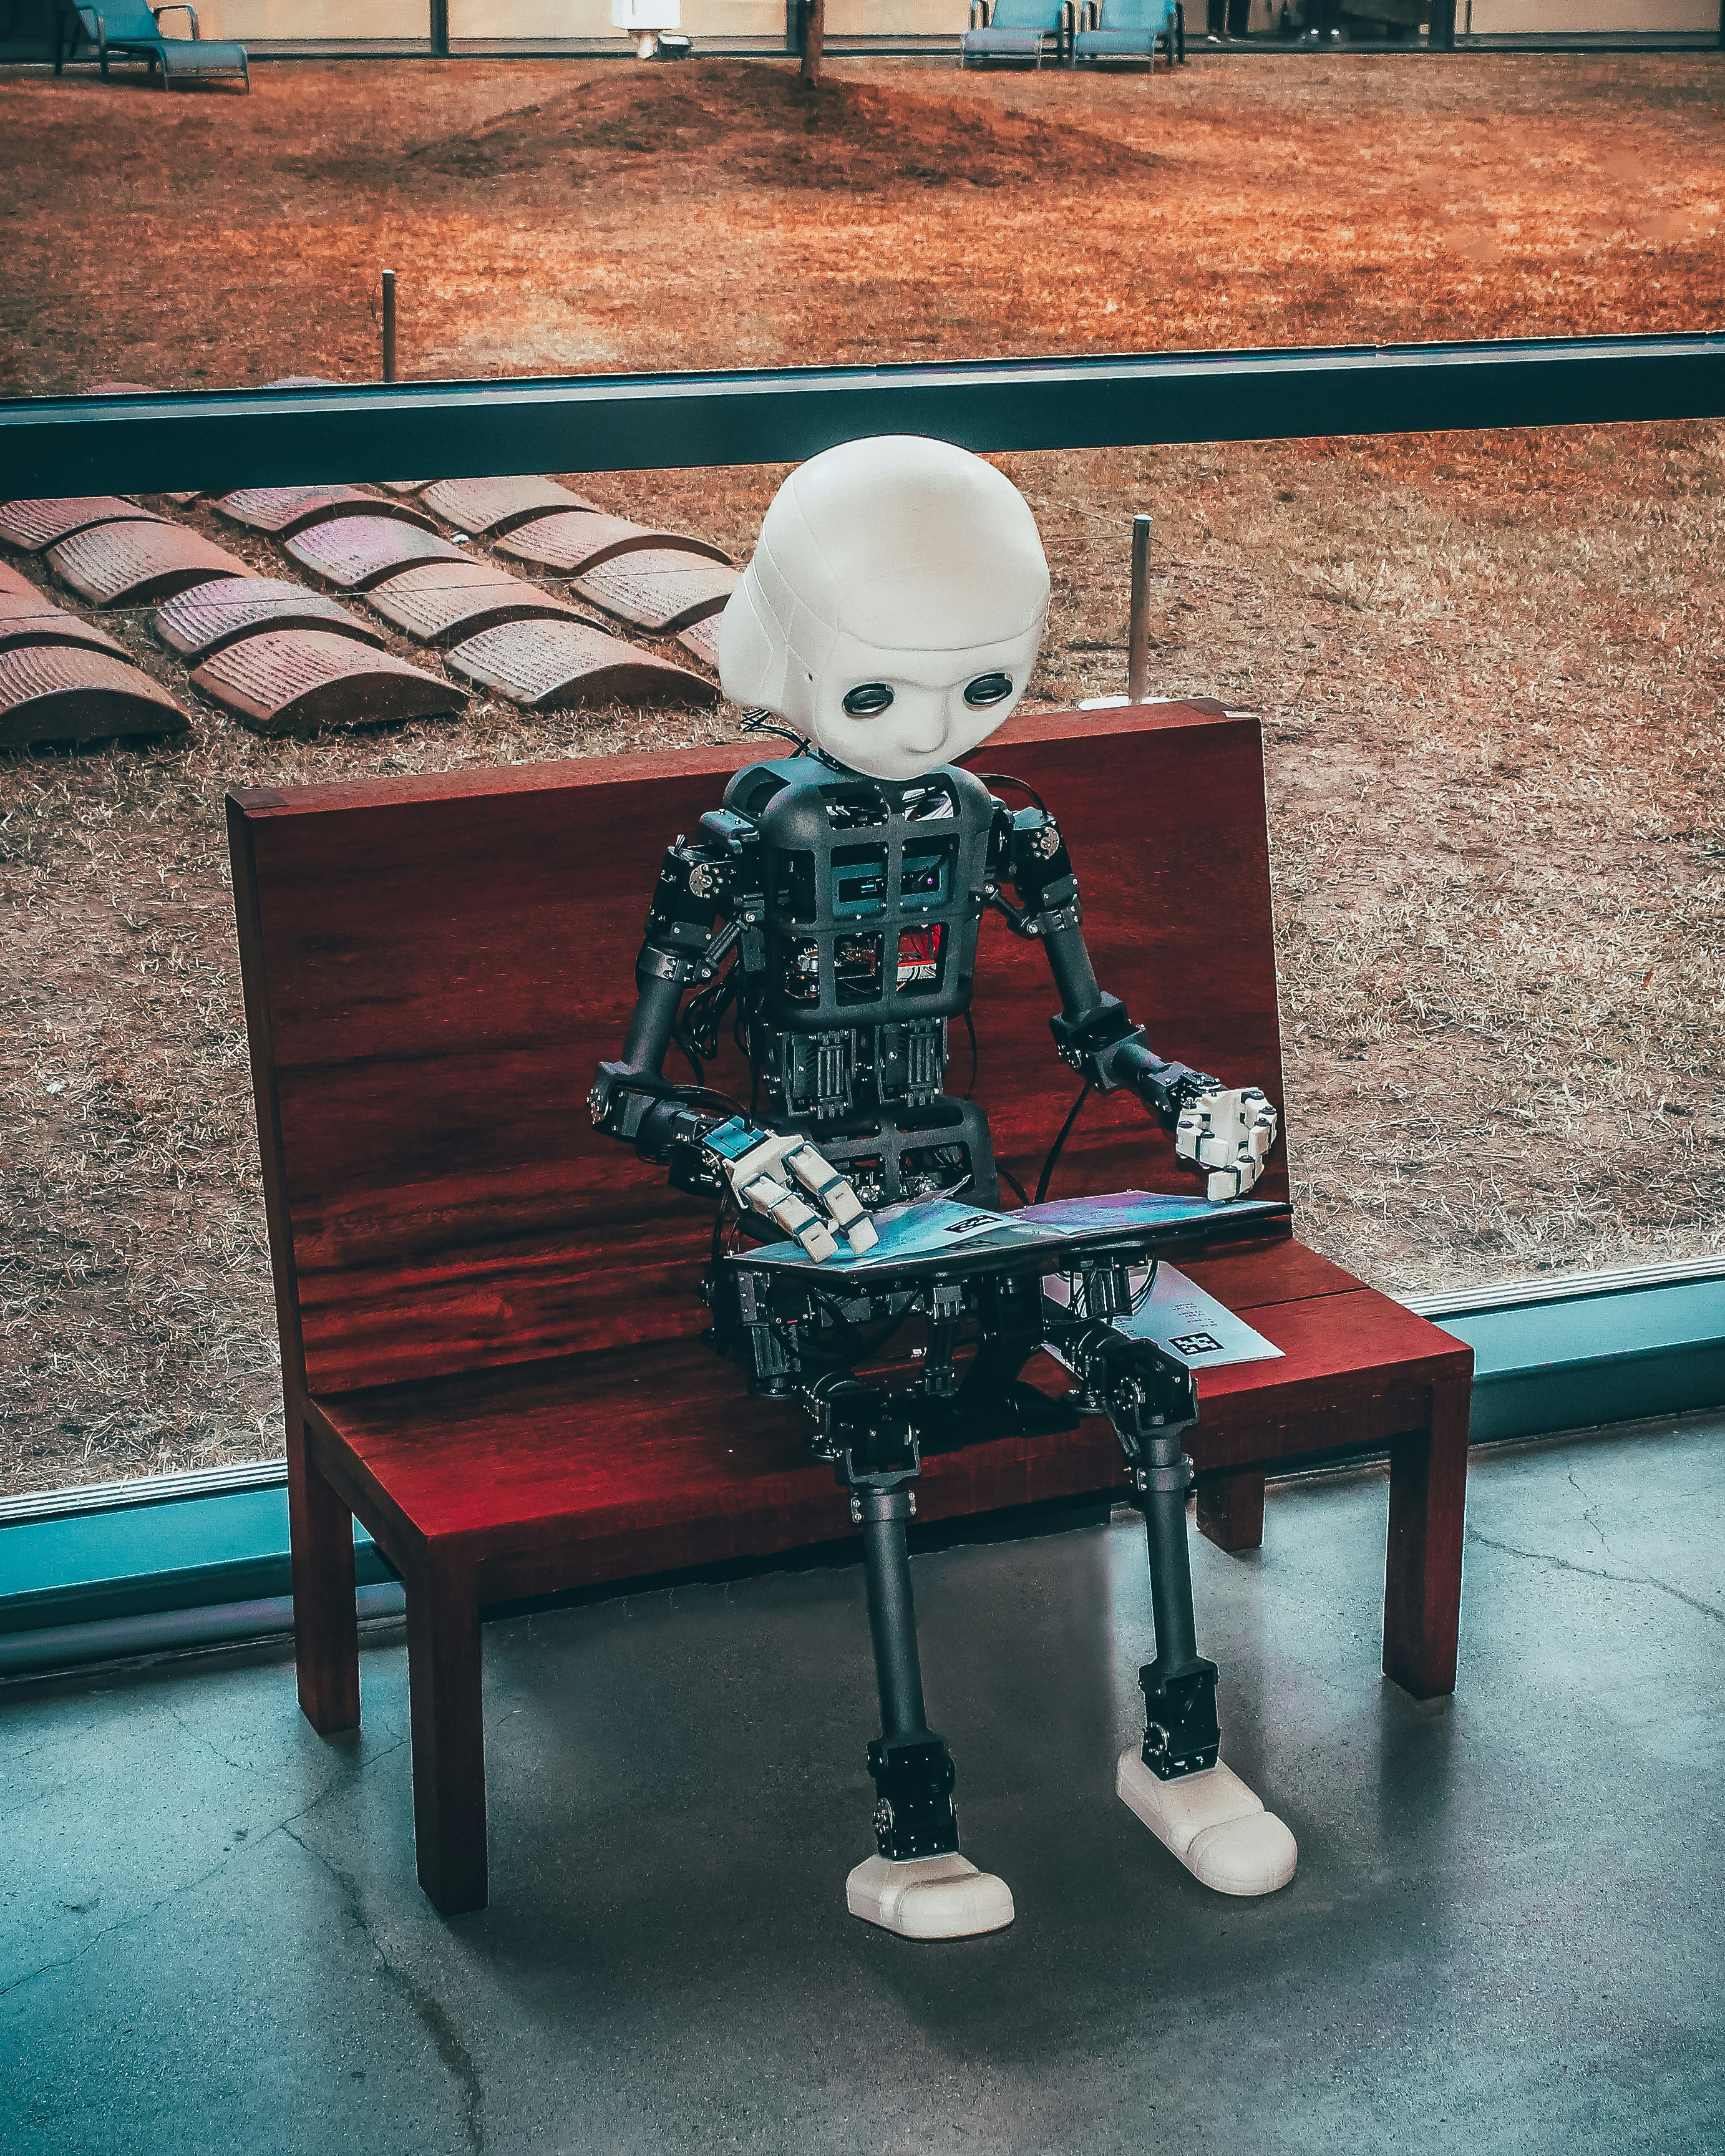
\includegraphics[width=\paperwidth,height=\paperheight]{cover-image}} % Image background
\centering
% \vspace*{2cm}
\par\normalfont\color{white}\fontsize{35}{35}\sffamily\selectfont
\textbf{AIML Notes - A2Z}
% {\LARGE A2Z}\par % Book title
% \vspace*{22.5cm}
~\vfill
\raggedleft
{\Huge Rohnak Agarwal}\\[-12pt]% Author name
{\centering \normalfont\fontsize{15}{15}\selectfont rrka79wal@gmail.com}\\
\endgroup
\restoregeometry

\newpage
~\vfill
\thispagestyle{empty}

\noindent Compiled Combined Notes of ALL subjects of \textbf{M.Tech. AIML} (BITS Pilani WILP) \\
Batch 2023-25

\vspace{0.5cm}

\noindent Mentor:\\
\textbf{Mr. Chintan Parikh} (\href{mailto:hi@chintan.io}{\texttt{hi@chintan.io}})\\
Associate Technical Manager - R\&D  (R\&D - Speech)\\
\textbf{Reverie Language Technologies}, Bangalore


\vspace{0.5cm}

\begin{customTableWrapper}{1.5}
\RaggedRight
\begin{table}[H]
    \centering
    \begin{tabular}{|p{4cm}|p{10cm}|}
        \hline

        \textbf{Master Google Drive Folder} & \url{https://drive.google.com/drive/folders/1j2vdpcchxFns7ifWEXbksAbQuDqqEFba?usp=drive_link} \\
        \hline\hline

        \customTableHeaderColor
        \multicolumn{2}{|c|}{\textbf{v1 Notes}} \\ \hline
        
        \textbf{Google Docs} & \url{https://docs.google.com/document/d/1CQLY3mfiy55zzP9l2v92sIKjKDCAgd06fPUrXxzNAKQ} \\ \hline\hline

        \customTableHeaderColor
        \multicolumn{2}{|c|}{\textbf{v2 Notes}} \\ \hline

        \textbf{Cover Image} & \textbf{Photo by} \href{https://unsplash.com/@santesson89?utm_content=creditCopyText&utm_medium=referral&utm_source=unsplash}{Andrea De Santis} \textbf{on} \href{https://unsplash.com/photos/black-and-white-robot-toy-on-red-wooden-table-zwd435-ewb4?utm_content=creditCopyText&utm_medium=referral&utm_source=unsplash}{Unsplash} \\

        \textbf{Code Repository} & \texttt{\url{https://github.com/rrkas/aiml-practice}} \\

        \textbf{\LaTeX \hspace{0.1cm} PDF src Code} & \texttt{\url{https://github.com/rrkas/AIML-Notes---A2Z-v2.0.0}} \\

        \textbf{OverLeaf Project} & \texttt{\url{https://www.overleaf.com/read/chtfnxbsnctz\#43c6ee}} \\

        \hline
    \end{tabular}
\end{table}
\end{customTableWrapper}

% \vspace{0.5cm}

\begin{customTableWrapper}{1.5}
\begin{table}[H]
    \centering
    
    \begin{tabular}{|c|p{6cm} >{\raggedleft\arraybackslash}p{6cm}|}
        \hline

        \customTableHeaderColor
        \multicolumn{3}{|c|}{\textbf{VERSIONS}} \\ \hline
        $\triangleright$ & \textbf{Day One} & \textit{April 21, 2024} \\ \hline
        
        \hline
        \customTableHeaderColor
        \multicolumn{3}{|c|}{\textbf{JOURNEY SO FAR}} \\ 
        
        \hline
        \textbf{v1} & google doc & \textit{April 21, 2024} \\
        
        \hline
        \textbf{v2} & OverLeaf/ \LaTeX \hspace{0.2cm} \textbf{(current)} & \textit{July 3, 2024} \\

        \hline
    \end{tabular}
\end{table}
\end{customTableWrapper}


PDF Generated on: \textit{\today} at \textbf{\currenttime\ IST}










\newgeometry{top=1.5cm, bottom=1cm, left=1.5cm, right=1.5cm}
\thispagestyle{empty}


\begin{center}
    \Huge Acknowledgement
    \vspace{0.5cm}
\end{center}

\begin{enumerate}
    \item I would like to thank \textbf{Birla Institute of Technology And Science, Pilani (BITS Pilani)} for providing me \textbf{Work Integrated Learning Program (WILP)} opportunity. Their rigorous and strict regime motivated me to do lot of self study and make this notes.

    \item I would also like to thank all my \textbf{M.Tech. colleagues} for supporting me and helping me through this challenging era.

    \item I would like to thank my mentor \textbf{Mr. Chintan Parikh}, for guidance, support and motivation throughout this time.

    \item I would like to thank \textbf{Reverie Language Technologies}, for permission, support and resources granted to me for persuing this course.
\end{enumerate}










\vspace{5cm}

\begin{center}
    \Huge Disclaimer
    \vspace{0.5cm}
\end{center}

\begin{enumerate}
    \item This document is purely made for the purpose of \textbf{comprehending} and \textbf{summarize} my journey in this M.Tech. program.

    \item The contents of this document are directly/ indirectly \textbf{COPIED} from various Books, Blogs, Research Papers, etc.

    \item The contents have been properly \textbf{CITED}.
\end{enumerate}


\restoregeometry



%----------------------------------------------------------------------------------------
%	TABLE OF CONTENTS
%----------------------------------------------------------------------------------------
\mainmatter
\pagenumbering{roman}
\pagestyle{empty} % No headers
\tableofcontents % Print the table of contents itself
\listoffigures
\listoftables
% \listoftheorems % TODO
\listofalgorithms
\lstlistoflistings
\chapter*{Mathematical Notations}

\section*{Brackets}

\begin{customTableWrapper}{1}
\begin{longtable}{|p{3cm}|p{12cm}|}
    \hline
    \customTableHeaderColor
    \textbf{Notation} & \textbf{Description/ Usage}\\ \hline
    \endfirsthead

    \hline
    \customTableHeaderColor
    \textbf{Notation} & \textbf{Description/ Usage}\\ \hline
    \endhead

    \hline
    \endfoot

    \hline
    \endlastfoot

    $<\cdots>$/ $\langle \cdots \rangle$ & \tableenumerate{
        \item Inner product
    }\\
    \hline

    $\dCurlyBrac{\cdots}$ & \tableenumerate{
        \item unordered set
        \item unordered basis: $\mathbf{B = \dCurlyBrac{b_1, \cdots , b_n}}$
    }\\
    \hline

    $(\cdots)$ & \tableenumerate{
        \item ordered set
        
        \item ordered basis: $\mathit{B} = \mathbf{(b_1, \cdots , b_n)}$ \fullref{ordered basis}
        
        \item $(a,b)$: range with \textbf{neither limits} included
    }\\
    \hline

    $(\cdots]$ & \tableenumerate{
        \item $(a,b]$: range with only \textbf{upper limit} included
    }\\
    \hline

    $[\cdots)$ & \tableenumerate{
        \item $[a,b)$: range with only \textbf{lower limit} included
    }\\
    \hline

    $[\cdots]$ & \tableenumerate{
        \item $[a,b]$: range with \textbf{both limits} included
        
        \item vectors (\fullref{vectors}) \& matrix
        \[
            \begin{bmatrix}
                x_{11} & \cdots & x_{1n}\\
                \vdots & \ddots & \vdots \\
                x_{m1} & \cdots & x_{mn}
            \end{bmatrix}
        \]

        \item $\mathbf{B = [b_1, \cdots , b_n]}$ is a matrix whose columns are the vectors $\mathbf{b_1, \cdots , b_n}$.
    }\\
    \hline

    $|\cdots|$ & \tableenumerate{
        \item \fullref{abs_value}
    }\\
    \hline

\end{longtable}
\end{customTableWrapper}


\section*{Operator}

\begin{customTableWrapper}{1}
\begin{longtable}{|p{3cm}|p{12cm}|}
    \hline
    \customTableHeaderColor
    \textbf{Operator} & \textbf{Description/ Usage}\\ \hline
    \endfirsthead

    \hline
    \customTableHeaderColor
    \textbf{Operator} & \textbf{Description/ Usage}\\ \hline
    \endhead

    \hline
    \endfoot

    \hline
    \endlastfoot

    $+$ & \tableenumerate{
        \item Addition
    }\\
    \hline

    $-$ & \tableenumerate{
        \item Subtraction
        
        \item \textbf{(Set) Difference}: $\mathbb{A}-\mathbb{B}$: It includes all the elements that are in set $\mathbb{A}$ but not in set $\mathbb{B}$.
        $\mathbb{A}-\mathbb{B}=\dCurlyBrac{ x | x \in \mathbb{A} \text{ and } x \not\in \mathbb{B} }$
    }\\
    \hline

    $a/b$ or $\dfrac{a}{b}$ or $\displaystyle\dfrac{a}{b}$ & \tableenumerate{
        \item Division (a divided by b)
        \item Or (a or b)
    }\\
    \hline

    $\times$ / $*$ / $\cdot$ & \tableenumerate{
        \item Multiplication
    }\\
    \hline

    $\cup$ & \tableenumerate{
        \item \textbf{Union}: $\mathbb{A}\cup\mathbb{B}$ means elements that are in either $\mathbb{A}$ or $\mathbb{B}$. 
        $\mathbb{A}\cup\mathbb{B}=\dCurlyBrac{ x | x \in \mathbb{A} \text{ or } x \in \mathbb{B} }$
    }\\
    \hline

    $\cap$ & \tableenumerate{
        \item \textbf{Intersection}: $\mathbb{A}\cup\mathbb{B}$ means elements that are in both $\mathbb{A}$ and $\mathbb{B}$.  
        $\mathbb{A}\cap\mathbb{B}=\dCurlyBrac{ x | x \in \mathbb{A} \text{ and } x \in \mathbb{B} }$
    }\\
    \hline

    $\backslash$ & \tableenumerate{
         \item \textbf{(Set) Difference}: $\mathbb{A}-\mathbb{B}$: It includes all the elements that are in set $\mathbb{A}$ but not in set $\mathbb{B}$.
        $\mathbb{A}\backslash\mathbb{B}=\dCurlyBrac{ x | x \in \mathbb{A} \text{ and } x \not\in \mathbb{B} }$
    }\\
    \hline

    $\cdots$ / $\vdots$ / $\ddots$ & \tableenumerate{
        \item to show a lot of elements
    }\\
    \hline

    $\mapsto$ & \tableenumerate{
        \item "Maps To"
    }\\
    \hline

    $\doubleuptack$ & \tableenumerate{
        \item conditional independence
    }


\end{longtable}
\end{customTableWrapper}


\section*{Symbols}

\begin{customTableWrapper}{1}
\begin{longtable}{|p{1.5cm}|p{3cm}|p{10cm}|}
    \hline
    \customTableHeaderColor
    \textbf{Symbol} & \textbf{Name} & \textbf{Description/ Usage}\\ \hline
    \endfirsthead

    \hline
    \customTableHeaderColor
    \textbf{Symbol} & \textbf{Name} & \textbf{Description/ Usage}\\ \hline
    \endhead

    \hline
    \endfoot

    \hline
    \endlastfoot

    
    $\pi$ / $\Pi$ & pi & \tableenumerate{
        \item $\displaystyle\pi \approx \dfrac{22}{7} \text{ or } \dfrac{355}{113} \text{ or } 3.1415926535$

        \item \( \dprod_{i=1}^{n} x_i = x_1 \cdot x_2 \cdots x_n \)
    
        \item \fullref{DRL: Policy}
    }\\
    \hline

    $e$ & Euler's number & \tableenumerate{
        \item \( \displaystyle e = \sum \limits _{n=0}^{\infty }{\frac {1}{n!}}\approx 2.71828 \)

        \item 
        
    }\\
    \hline

    $\alpha$ & Alpha & \tableenumerate{
        \item \fullref{Coordinate vector}
    }\\
    \hline


    $\beta$ & Beta & \tableenumerate{
        \item  
    }\\
    \hline

    $\gamma$ / $\Gamma$ & Gamma & \tableenumerate{
        \item \fullref{Gamma Function}
    }\\
    \hline

    $\sigma$ / $\Sigma$ & Sigma & \tableenumerate{
        \item $\dsum_{i=1}^{n} x_i= x_1 + x_2 + \cdots + c_n$
        \item \fullref{Logistic function}
    }\\
    \hline

    $\phi$ / $\Phi$ & Phi & \tableenumerate{
        \item \fullref{Linear Mappings/ vector space homomorphism/ linear transformation}
    }\\
    \hline

    $\psi$ / $\Psi$ & Psi & \\
    \hline

    $\epsilon$ & epsilon & \tableenumerate{
        \item Exploration: \fullref{Exploration vs. Exploitation}
    }\\
    \hline

    $\eta$ & Eta & \tableenumerate{
        \item Learning Rate
    } \\
    \hline

    $\delta$ / $\Delta$ & Delta & \tableenumerate{
        \item \fullref{Difference Quotient}
        \item \textbf{Symmetric (Set) Difference/ disjunctive union/ set sum}\indexlabel{Symmetric (Set) Difference/ disjunctive union/ set sum}: $\mathbb{A}\Delta\mathbb{B} = (\mathbb{A}-\mathbb{B})\cup(\mathbb{B}-\mathbb{A})$ 
    } \\
    \hline

    $\theta$ / $\Theta$ & Theta & \tableenumerate{
        \item angles:
        \begin{enumerate}
            \item\fullref{Trigonometric functions}
            \item\fullref{Inverse trigonometric functions}
            \item\fullref{Hyperbolic functions}
        \end{enumerate}
    }\\
    \hline

    $\xi$ / $\Xi$ & Xi & \\
    \hline

    $\chi$ & Chi & \\
    \hline

    $\omega$ / $\Omega$ & Omega & \\
    \hline


    $\lambda$ / $\Lambda$ & Lambda & \\
    \hline

    $\nabla$ & Nabla & \tableenumerate{
        \item $\nabla F(x)$: Gradient of the function $F(x)$ wrt $x$
    }\\
    \hline

    $\exists$ & Exists & \tableenumerate{
        \item Example: $\exists a, a<10$ : there exists a such that "a" is less than 10
    }\\
    \hline

    $\forall$ & For all & \tableenumerate{
        \item Example: $\forall a \in \mathbb{A}$ : for all "a" in $\mathbb{A}$ 
    }\\
    \hline

    $\kappa$ & Kappa & \tableenumerate{
        \item Cohen’s Kappa Statistic
    }\\
    \hline

    $\nu$ & Nu & 
    \\
    \hline

\end{longtable}
\end{customTableWrapper}


\section*{Alphabetical Notations}

\begin{customTableWrapper}{1}
\begin{longtable}{|p{3cm}|p{12cm}|}
    \hline
    \customTableHeaderColor
    \textbf{Notation} & \textbf{Description/ Usage}\\ \hline
    \endfirsthead

    \hline
    \customTableHeaderColor
    \textbf{Notation} & \textbf{Description/ Usage}\\ \hline
    \endhead

    \hline
    \endfoot

    \hline
    \endlastfoot


    $a$, $b$, $a_i$ & \tableenumerate{
        \item scalar
    }\\
    \hline

    $\mathbf{a}$, $\mathbf{b}$, $\mathbf{a}_i$, $\mathbf{v}^\top$ & \tableenumerate{
        \item \fullref{vectors}
    }\\
    \hline

    $\mathbf{A}$, $\mathbf{B}$, $\mathbf{M}^\top$ & \tableenumerate{
        \item matrix
        \item vector space
    }\\
    \hline

    $\mathbb{A}$, $\mathbb{B}$, $\mathbb{R}$, $\mathbb{R}^{m\times n}$ & \tableenumerate{ 
        \item set

        \item $\mathbb{E}$: Expected value
        
        \item $\mathbb{U}$: Universal set (set theory)
        
        \item $\mathbbm{1}$: \fullref{Indicator function}
    }\\
    \hline



    
\end{longtable}
\end{customTableWrapper}




\cleardoublepage % Forces the first chapter to start on an odd page so it's on the right
\pagestyle{fancy} % Print headers again
\cleardoublepage

%----------------------------------------------------------------------------------------
%	CHAPTERs
%----------------------------------------------------------------------------------------

\mainmatter
\pagenumbering{arabic}
\cleardoublepage
\begin{justify}
    
    \chapter{Common Functions \& Operators: Math}



\section{Absolute Value ( $\dabs{x}$ )}\label{abs_value}
\[
    \dabs{ x } = \begin{cases}
       x & \text{ if } x \geq 0 \\
       -x & \text{ if } x < 0 
    \end{cases}
\]


\section{Factorial ( $x!$ )}\label{Factorial}
\[
    x! = \prod_{i=1}^{x} i = 1 \cdot 2 \cdots (x-1) \cdot x 
\]

\section{Combination ( $C(n,r)$ / $^nC_r$ / $nCr$ ) } \label{Combination}

\[
    C(n,r) = ^nC_r = nCr = \displaystyle\binom{n}{r} = \displaystyle\dfrac{n!}{(n-r)!r!}
\]

\section{Permutation \( \dParenBrac{\ P(n,r)\ /\ ^nP_r\ /\ nPr\ } \)} \label{Permutation}

\[
    P(n,r) = ^nP_r = nPr = \displaystyle\dfrac{n!}{(n-r)!}
\]

\section{Exponential Function ( $exp(x)$ )}\label{Exponential Function}

\[
    exp(x) = e^x
\]

\section{Gamma Function ( $\Gamma(x)$ )}\label{Gamma Function}

\[
    \Gamma(x) = \dint_{0}^{\infty} t^{x-1} e^{-t} dt
\]


\section{Logarithm Function ( $\log(x)$ / $\ln(x)$ )}\label{Logarithm Function}
\[
    y = \log_a(x) \Leftrightarrow x = a^y
\]

Natural Logarithm Function ($a=e$):
\[
    y = \ln(x) \Leftrightarrow x = e^y
\]


\section{Sign Function ( $\rcmdXsgn(x)$ )}\label{Sign Function}
\begin{align*}
    \rcmdXsgn(x) = \begin{cases}
         1 & \text{ if } x > 0 \\
         0 & \text{ if } x = 0 \\
         -1 & \text{ if } x < 0 
        \end{cases}
\end{align*}



\section{Indicator function ( $\mathbbm{1}_x$ )}\label{Indicator function}

\begin{align*}
    \mathbbm{1}_x = {\begin{cases}
        1 & \text{ if x is true } \\
        0 & \text{ if x is false }
    \end{cases}}
\end{align*}

\section{Infinite Step Function ( $1(z)$ )}

\begin{align*}
    1(z) = {\begin{cases}
        0 & \text{ if } z \leq 0 \\
        \infty & \text{ otherwise }
    \end{cases}}
\end{align*}

This gives infinite penalty if the constraint is not satisfied.


\section{Trigonometric functions - TODO \cite{wiki-Trigonometric_functions}}\label{Trigonometric functions}

\begin{table}[H]
    \centering
    \begin{minipage}[t]{0.3\linewidth}
        \begin{figure}[H]
            \centering
            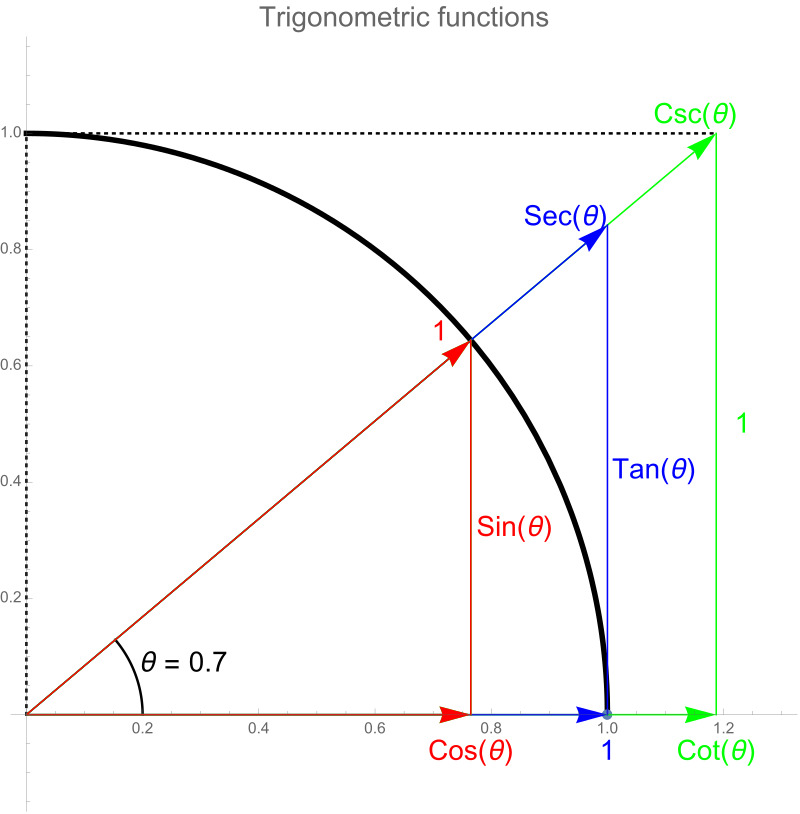
\includegraphics[height=4.5cm]{Pictures/maths/TrigFunctions.jpg}
            \caption{Trigonometry Functions Comparison}
        \end{figure}
    \end{minipage}
    \hfill
    \begin{minipage}[t]{0.3\linewidth}
        \begin{figure}[H]
            \centering
            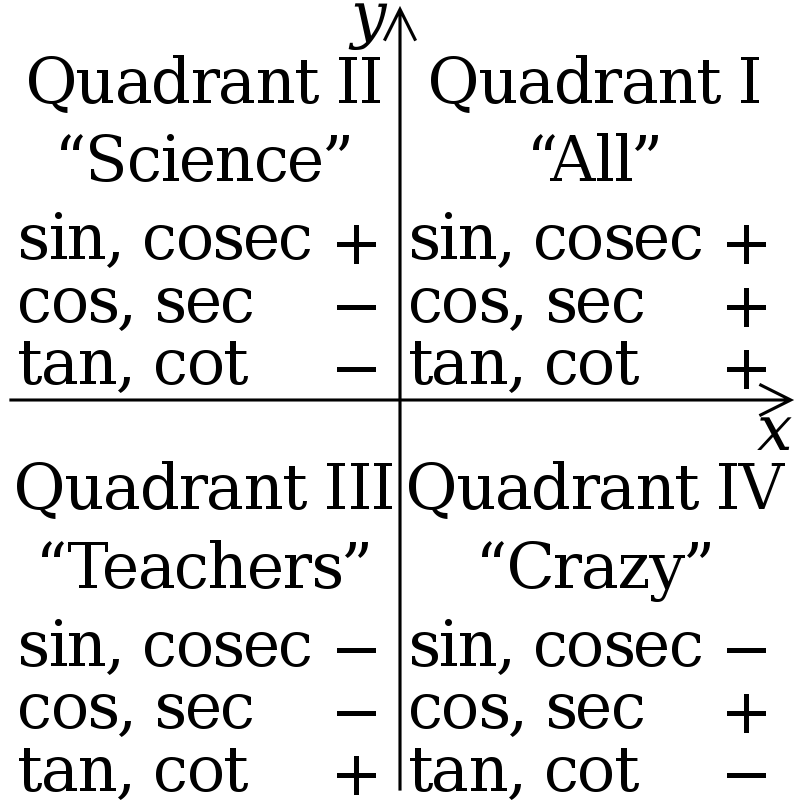
\includegraphics[height=4.5cm]{Pictures/maths/Trigonometric_function_quadrant_sign.png}
            \caption{Trigonometry Quadrant Signs}
        \end{figure}
    \end{minipage}
    \begin{minipage}[t]{0.3\linewidth}
        \begin{figure}[H]
            \centering
            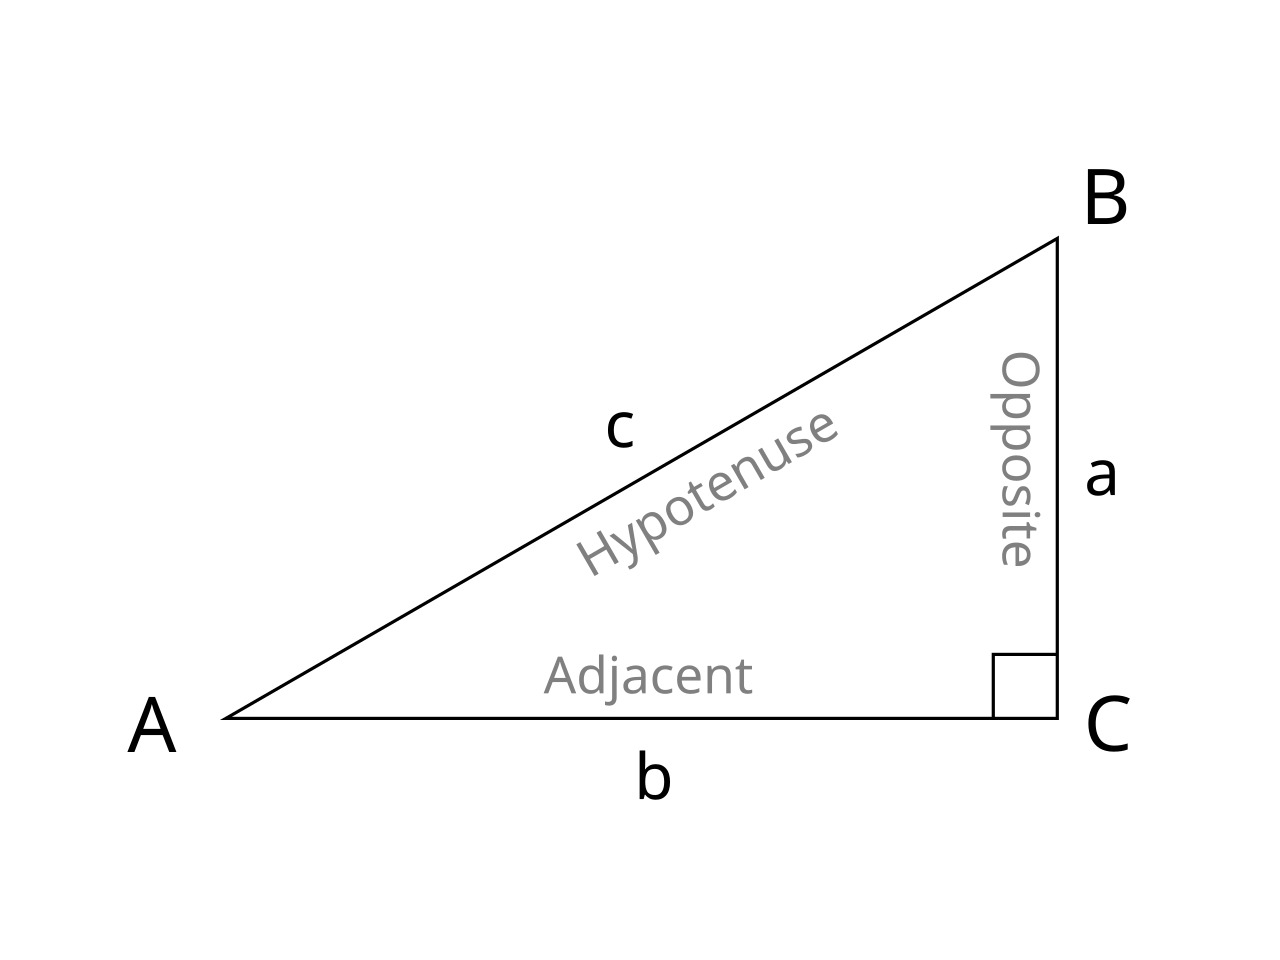
\includegraphics[height=4.5cm]{Pictures/maths/TrigonometryTriangle.jpg}
            \caption{Trigonometry Triangle}
        \end{figure}        
    \end{minipage}
\end{table}

\subsection{sine ( $\sin(\theta)$ )}\label{sine (sin)}

\[
    \sin(\theta) = \displaystyle \dfrac{\mathrm{opposite}}{\mathrm{hypotenuse}}
\]
\[    \sin(\theta + 2k\pi) = \sin(\theta)   \]

\subsection{cosine ( $\cos(\theta)$ )}\label{cosine (cos)}

\[
    \cos(\theta) = \displaystyle\dfrac{\mathrm {adjacent} }{\mathrm {hypotenuse} }
\]
\[  \cos(\theta + 2k\pi ) = \cos(\theta)  \]

\subsection{tangent ( $\tan(\theta)$ )}\label{tangent (tan)}

\[
    \tan(\theta) =\displaystyle \dfrac {\mathrm {opposite} }{\mathrm {adjacent} }
\]
\[  \tan(\theta + k\pi ) = \tan(\theta)  \]

\subsection{cosecant ( $\csc(\theta)$ }\label{cosecant (csc)}
\[
    \csc(\theta) =\displaystyle\dfrac {\mathrm {hypotenuse} }{\mathrm {opposite} }
\]

\subsection{secant ( $\sec(\theta)$ )}\label{secant (sec)}
\[
    \sec(\theta) =\displaystyle\dfrac {\mathrm {hypotenuse} }{\mathrm {adjacent} }
\]

\subsection{cotangent ( $\cot(\theta)$ )}\label{cotangent (cot)}

\[
    \cot(\theta) =\displaystyle\dfrac {\mathrm {adjacent} }{\mathrm {opposite} }
\]
\[  \cot(\theta + k\pi ) = \cot(\theta)  \]


\subsection{Properties \& Formulas}
\begin{enumerate}
    \item \( \sin^2(\theta) + \cos^2(\theta) = 1 \)
\end{enumerate}


\section{Inverse trigonometric functions - TODO \cite{wiki-Inverse_trigonometric_functions}}\label{Inverse trigonometric functions}

\section{Hyperbolic Functions \cite{wiki-Hyperbolic_functions}}\label{Hyperbolic functions}


\begin{table}[H]
    \centering
    \begin{minipage}[t]{0.45\linewidth}
        \begin{figure}[H]
            \centering
            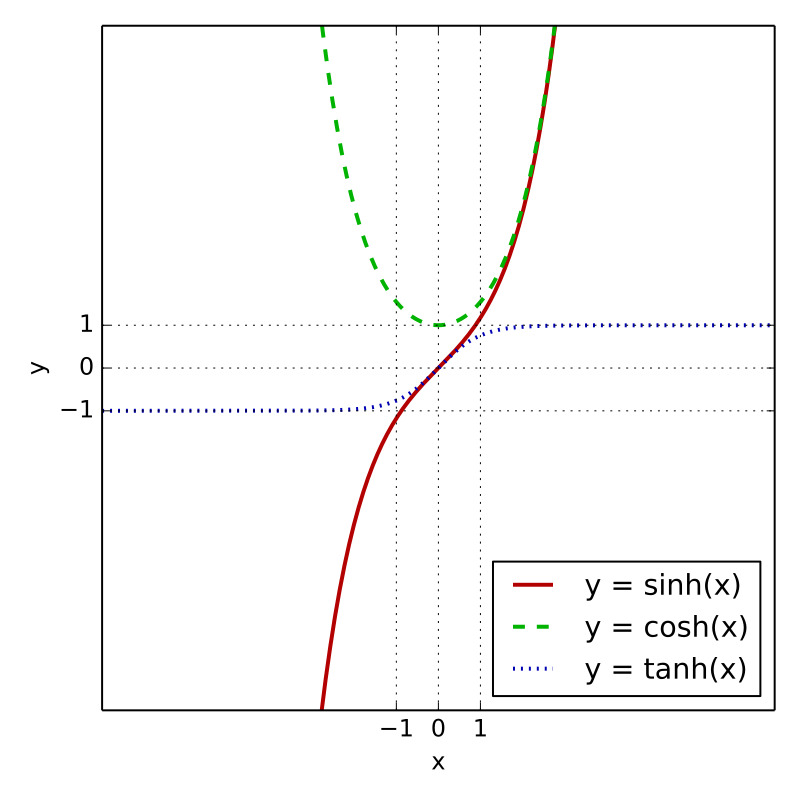
\includegraphics[height=7.5cm]{Pictures/maths/Sinh_cosh_tanh.jpg}
            \caption{$\sinh(x)$, $\cosh(x)$ \& $\tanh(x)$}
        \end{figure}        
    \end{minipage}
    \hfill
    \begin{minipage}[t]{0.45\linewidth}
        \begin{figure}[H]
            \centering
            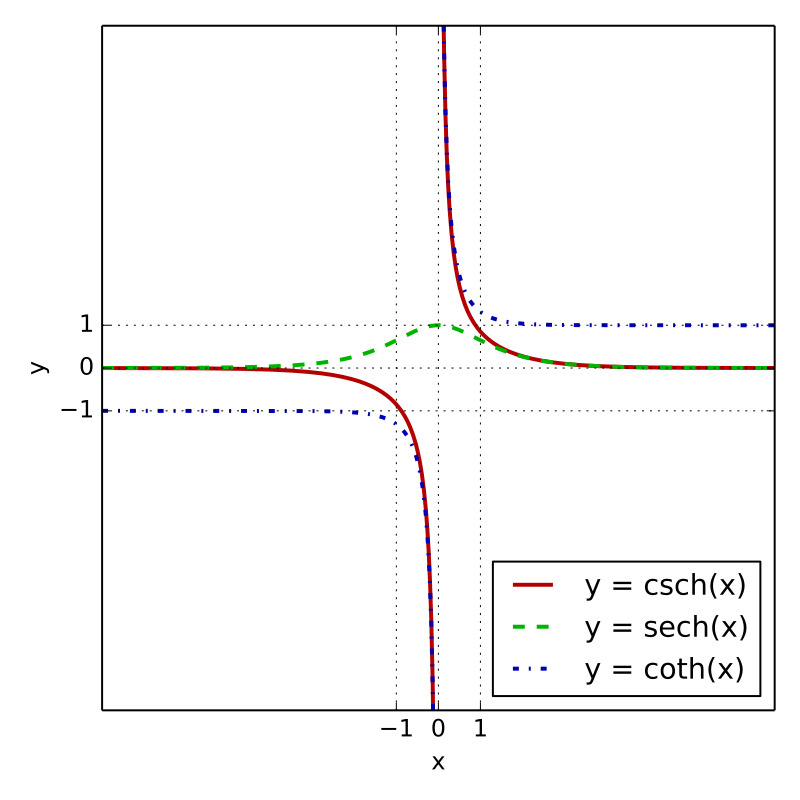
\includegraphics[height=7.5cm]{Pictures/maths/Csch_sech_coth.jpg}
            \caption{$\rcmdXcsch(x)$, $\rcmdXsech(x)$ \& $\coth(x)$}
        \end{figure}
    \end{minipage}
\end{table}

\subsection{Hyperbolic sine ( $\sinh(x)$ ) }\label{Hyperbolic sine (sinh)}
\[
    (\sinh(x) = {\displaystyle\dfrac{e^{x} - e^{-x}}{2}}={\displaystyle\dfrac{e^{2x} - 1}{2e^{x}}}={\displaystyle\dfrac{1 - e^{-2x}}{2e^{-x}}}
\]

\subsection{Hyperbolic cosine ( $\cosh(x)$ ) }\label{Hyperbolic cosine (cosh)}
\[
    \cosh(x) = {\displaystyle\dfrac{e^{x} + e^{-x}}{2}} = {\displaystyle\dfrac{e^{2x} + 1}{2e^{x}}} = {\displaystyle\dfrac{1 + e^{-2x}}{2e^{-x}}}
\]

\subsection{Hyperbolic tangent ( $\tanh(x)$ )}\label{Hyperbolic tangent (tanh)}
\[
    \tanh(x) = \displaystyle\dfrac{\sinh(x)}{\cosh(x)} = \displaystyle\dfrac{e^{x} - e^{-x}}{e^{x} + e^{-x}} = \displaystyle\dfrac{e^{2x} - 1}{e^{2x} + 1}
\]

\subsection{Hyperbolic cotangent ( $\coth(x)$ )}\label{Hyperbolic cotangent (coth)}
\[
    \coth(x) = \displaystyle\dfrac{1}{\tanh(x)} = \displaystyle\dfrac{\cosh(x)}{\sinh(x)} = \displaystyle\dfrac{e^{x} + e^{-x}}{e^{x} - e^{-x}} = \displaystyle\dfrac{e^{2x} + 1}{e^{2x} - 1}
\]

$x \neq 0$

\subsection{Hyperbolic secant ( $\rcmdXsech(x)$ )} \label{Hyperbolic secant (sech)}
\[
    \rcmdXsech(x) = \displaystyle\dfrac{1}{\cosh(x)} = \displaystyle\dfrac{2}{e^{x} + e^{-x}} = \displaystyle\dfrac{2e^{x}}{e^{2x} + 1}
\]

\subsection{Hyperbolic cosecant ( $\rcmdXcsch(x)$ )}\label{Hyperbolic cosecant (csch)}
\[
    \rcmdXcsch(x) = \displaystyle\dfrac{1}{\sinh(x)} = \displaystyle\dfrac{2}{e^{x} - e^{-x}} = \displaystyle\dfrac{2e^{x}}{e^{2x} - 1}
\]
$x \neq 0$

\subsection{Properties \& Formulas}

\begin{customTableWrapper}{1}
\begin{table}[H]
    \centering
    \begin{tabular}{|c|r|r|r|r|r|r|}
        \hline
        $\theta$ & $\sinh(\theta)$ & $\cosh(\theta)$ & $\tanh(\theta)$ & $\coth(\theta)$ & $\rcmdXsech(\theta)$ & $\rcmdXcsch(\theta)$ \\ \hline

        $-\theta$ & $-\sinh(\theta)$ & $\cosh(\theta)$ & $-\tanh(\theta)$ & $-\coth(\theta)$ & $\rcmdXsech(\theta)$ & $-\rcmdXcsch(\theta)$ \\ \hline
    \end{tabular}
    \caption{Hyperbolic angles}
\end{table}
\end{customTableWrapper}


\section{Softmax function/ softargmax ( $\sigma (\mathbf {z})$ ) \cite{wiki-softmax-function,dnn-1}} \label{Softmax function}
\begin{enumerate}
    \item The softmax function, also known as softargmax or normalized exponential function, converts a vector of $K$ real numbers into a probability distribution of $K$ possible outcomes. 
    
    \item It is a generalization of the logistic function to multiple dimensions, and used in multinomial logistic regression. 
    
    \item The softmax function is often used as the last activation function of a neural network to normalize the output of a network to a probability distribution over predicted output classes.

    \item $
        {\displaystyle \sigma (\mathbf {z} )_{i}={\displaystyle\dfrac {\exp({z_{i}})}{\dsum _{j=1}^{K} \exp({z_{j}})}}}
    $\\
    Where:
    \[
        {\displaystyle \sigma \colon \mathbb {R} ^{K}\to (0,1)^{K}}
        \hfill
        {\displaystyle K\geq 1}
    \]
    \[
        {\displaystyle \mathbf {z} =(z_{1},\dotsc ,z_{K})\in \mathbb {R} ^{K}}
    \]

    \item \textbf{numerical overflow}: If some of the $z_j$ are very large, i.e., very positive, then $\exp(z_j)$ might be larger than the largest number we can have for certain data types. This is called overflow.
    
    \item \textbf{numerical underflow}: if every argument is a very large negative number, we will get underflow.
    
    \item A way round this problem is to subtract $\bar{o} \stackrel{\textrm{def}}{=} \max_k o_k$ from all entries:
    \[
        \hfill
        \hat y_j 
        = \dfrac{\exp (o_j)}{\dsum_k \exp (o_k)} 
        = \dfrac{\exp(o_j - \bar{o}) \exp (\bar{o})}{\dsum_k \exp (o_k - \bar{o}) \exp (\bar{o})} 
        = \dfrac{\exp(o_j - \bar{o})}{\dsum_k \exp (o_k - \bar{o})}
        \hfill
        (o_j - \bar{o} \leq 0 \quad \forall j)
    \]
    denominator: $\in [1, q]$\\
    numerator: $\leq 1$ \\
    \[
        \hfill
        \log (\hat{y}_j )
        = \log \dParenBrac{\dfrac{\exp(o_j - \bar{o})}{\dsum_k \exp (o_k - \bar{o})} }
        = o_j - \bar{o} - \log \dParenBrac{\dsum_k \exp (o_k - \bar{o})}
        \hfill
    \]
    
\end{enumerate}


\section{Convolution ( $(f * g)(\mathbf{x})$ ) \cite{dnn-1}} \label{function: Convolution}

\begin{enumerate}
    \item In mathematics, the convolution between two functions, say $f, g: \mathbb{R}^d \to \mathbb{R}$ is defined as:
    \[
        \hfill
        (f * g)(\mathbf{x}) = 
        \begin{cases}
            \dint f(\mathbf{z}) g(\mathbf{x}-\mathbf{z}) d\mathbf{z} & \text{ (continuous)} \\[1ex]
            \dsum_\mathbf{z} f(\mathbf{z}) g(\mathbf{x}-\mathbf{z}) & \text{ (discrete)} \\
        \end{cases}
        \hfill
    \]
    we measure the overlap between $f$ and $g$ when one function is “\textbf{flipped}” and \textbf{shifted} by $\mathbf{x}$

    \item For two-dimensional tensors, we have a corresponding sum with indices $(a, b)$ for $f$ and $(i - a, j - b)$ for $g$:
    \[
        \hfill
        (f * g)(i, j) = \dsum_a\dsum_b f(a, b) g(i-a, j-b)
        \hfill
    \]
\end{enumerate}














































    \chapter{Calculus}

\section{Difference Quotient ( $\displaystyle\frac{\delta y}{\delta x}$ )}\label{Difference Quotient}

\begin{table}[H]
    \begin{minipage}{0.39\linewidth}
        \begin{figure}[H]
            \centering
            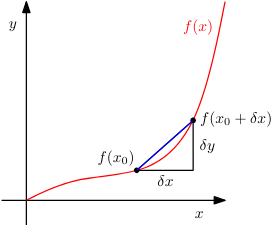
\includegraphics[height=4cm]{Pictures/maths/Difference Quotient.png}
            \caption{Difference Quotient}
        \end{figure}
    \end{minipage}
    \hfill
    \begin{minipage}{0.59\linewidth}
        \begin{enumerate}
            \item The difference quotient \( \displaystyle\dfrac{\delta y}{\delta x} = \displaystyle\dfrac{f(x + \delta x) - f(x)}{\delta x} \) computes the slope of the secant line through two points on the graph of $y = f(x)$. 
            
            \item The difference quotient can also be considered the average slope of $f$ between $x$ and $x + \delta x$ if we assume $f$ to be a linear function. 
            
            \item In the limit for $\delta x \rightarrow 0$, we obtain the tangent of $f$ at $x$, if $f$ is differentiable.

        \end{enumerate}
    \end{minipage}
\end{table}



\section{Derivative ( $\displaystyle\frac{dy}{dx}$ / $y'$)}\label{Derivative}

For $h > 0$ the derivative of $y = f(x)$ at $x$ is defined as the limit \( \displaystyle\dfrac{\delta y}{\delta x} = \lim_{h\rightarrow 0}\displaystyle\dfrac{f(x + h) - f(x)}{h} \) and the secant becomes a tangent.

\subsection{Sum rule}
\[
    (f(x) + g(x))' = f'(x) + g'(x)
\]

\subsection{Product rule}
\[
    (f(x)g(x))' = f'(x)g(x) + f(x)g'(x)
\]

\subsection{Chain rule}
\[
    g(f(x))' = (g \circ f)'(x) = g'(f(x))f'(x)
\]

\subsection{Quotient rule}
\[
    \left( \displaystyle\dfrac{f(x)}{g(x)} \right)' = \displaystyle\dfrac{[f'(x)g(x) - f(x)g'(x)]}{(g(x))^2}
\]

\section{Power Series}\label{Power Series}
\[
    f(x) = \sum_{k=0}^{\infty} a_k (x-c)^k
\]
where $a_k$ are coefficients and $c$ is a constant

\section{Taylor Polynomial ( $T_n(x)$ )}\label{Taylor Polynomial}
The Taylor polynomial of degree $n$ of $f : \mathbb{R} \rightarrow \mathbb{R}$ at $x_0$ is defined as: 
\[
    T_n(x) = \sum_{k=0}^{n}\displaystyle\dfrac{f^{(k)}(x_0)}{k!}(x-x_0)^k
\]
where, $f^{(k)}(x_0)$ is the $k$th derivative of $f$ at $x_0$ and $\displaystyle\dfrac{f^{(k)}(x_0)}{k!}$ are the coefficients of the polynomial.


\section{Multivariate Taylor Polynomial}\label{Multivariate Taylor Polynomial}
The Taylor polynomial of degree $n$ of $f$ at $x0$ contains the first $n + 1$ components of the series and is defined as:
\[
    f(x) = \sum_{k=0}^{n} \displaystyle\dfrac{D_x^k f(x_0)}{k!}\delta^k
\]

where, $D_x^kf(x_0)$ is the $k$-th (total) derivative of $f$ with respect to $x$, evaluated at $x_0$.

$k$th-order tensor \( \delta^k \in \mathbb{R}^{\overset{k \text{ times}}{\overbrace{D \times D \times \cdots \times D}}} \) is obtained as a $k$-fold outer product, denoted by $\bigotimes$, of the vector $\delta \in \mathbb{R}^D$

\begin{table}[H]
    \centering
    \begin{tabular}{l l}
        \( \delta^2 := \delta\bigotimes\delta = \delta\delta^\top \) & \( \delta^2[i, j] = \delta [i]\delta [j] \) \\
        \( \delta^3 := \delta\bigotimes\delta\bigotimes\delta \) & \( \delta^3[i, j, k] = \delta [i]\delta [j]\delta [k] \) \\
    \end{tabular}
\end{table}

$D_x^kf(x_0)\delta k$ contains $k$-th order polynomial:
\begin{table}[H]
    \begin{tabular}{l l}
        $k = 0$ & $D_x^0f(x_0)\delta^0 = f(x_0) \in \mathbb{R}$ \\
         
        $k = 1$ & \( D_x^1f(x_0)\delta^1 = \underbrace{\nabla_xf(x_0)}_{1\times D} \underbrace{\delta}_{D \times 1} = \dsum_{i=1}^{D} \nabla_xf(x_0)[i]\delta [i] \in \mathbb{R} \) \\

        $k = 2$ & \( D_x^2f(x_0)\delta^2 = \operatorname{tr}(\underbrace{H(x_0)}_{D\times D} \underbrace{\delta}_{D \times 1} \underbrace{\delta^\top}_{1 \times D}) = \delta^\top H(x_0)\delta = \dsum_{i=1}^{D}\dsum_{j=1}^{D} H[i,j]\delta [i]\delta [j] \in \mathbb{R} \) \\

        $k = 3$ & \( D_x^3f(x_0)\delta^3 = \dsum_{i=1}^{D} \dsum_{j=1}^{D} \dsum_{k=1}^{D} D_x^3f(x_0)[i,j,k]\delta [i] \delta [j] \delta [k] \in \mathbb{R} \) \\
         
    \end{tabular}
\end{table}

$H(x_0)$ is the \textbf{Hessian} of $f$ evaluated at $x_0$.


\section{Taylor Series ( $T_\infty(x)$ )}\label{Taylor Series}
For a smooth function $f \in C^\infty$, $f : \mathbb{R} \rightarrow \mathbb{R}$, the taylor series of $f$ at $x_0$ is defined as:

\[
    T_\infty(x) = \sum_{k=0}^{\infty}\displaystyle\dfrac{f^{(k)}(x_0)}{k!}(x-x_0)^k
\]

SEE: \fullref{Taylor Polynomial}
\begin{enumerate}
    \item $f^{(k)}(x_0)$ is the $k$th derivative of $f$ at $x_0$

    \item For $x_0 = 0$, we obtain the \textbf{Maclaurin series}\indexlabel{Maclaurin series} as a special instance of the Taylor series. 
    
    \item If $f(x) = T_\infty(x)$, then $f$ is called \textbf{analytic}\indexlabel{analytic}.
    
    \item $f \in C^\infty$ means that $f$ is continuously differentiable infinitely many times.

    \item a Taylor polynomial of degree $n$ is an approximation of a function, which does not need to be a polynomial

    \item The Taylor polynomial is similar to $f$ in a neighborhood around $x_0$. However, a Taylor polynomial of degree $n$ is an exact representation of a polynomial $f$ of degree $k \leq n$ since all derivatives $f(i)$, $i > k$ vanish.

    \item it is a special case of \textbf{power series}(SEE: \fullref{Power Series}).

\end{enumerate}


\section{Multivariate Taylor Series}\label{Multivariate Taylor Series}

SEE: \fullref{Multivariate Taylor Polynomial}\\
We consider a function $f : \mathbb{R}^D \rightarrow \mathbb{R}$, $x \rightarrow f(x)$, $x \in \mathbb{R}^D$, that is smooth at $x_0$. When we define the difference vector $\delta := x - x_0$, the multivariate Taylor series of $f$ at $x_0$ is defined as
\[
    f(x) = \sum_{k=0}^{\infty} \displaystyle\dfrac{D_x^k f(x_0)}{k!}\delta^k
\]

where, $D_x^kf(x_0)$ is the $k$-th (total) derivative of $f$ with respect to $x$, evaluated at $x_0$.































































































    \chapter{Linear Algebra \cite{mfml-1}}

\section{Groups ( $G = (\mathbb{G}, \otimes)$ ) \cite{mfml-1}}\label{lin-alg-Groups}

Consider a set $\mathbb{G}$ and an operation $\otimes$ : $\mathbb{G} \times \mathbb{G} \to \mathbb{G}$ group defined on $\mathbb{G}$. Then $G := (\mathbb{G}, \otimes)$ is called a group if the following hold:

\begin{table}[H]
    \begin{tabular}{l p{10cm}}
        Closure of $\mathbb{G}$ under $\otimes$ & $\forall x,y \in \mathbb{G} : x \otimes y \in \mathbb{G}$ \\
        Associativity & $\forall x,y,z \in \mathbb{G}:(x \otimes y) \otimes z = x \otimes (y \otimes z) $ \\
        Neutral Element & $\exists e \in \mathbb{G} \text{ , } \forall x\in \mathbb{G}: x \otimes e = e \otimes x = x$ \\
        Inverse Element & $\forall x\in \mathbb{G} \text{ , } \exists y \in \mathbb{G}: x\otimes y = y\otimes x = e$ where $e$ is the neutral element. ( $y = x^{-1}$ and $x = y^{-1}$ ) \\
    \end{tabular}
\end{table}

\begin{enumerate}
    \item Inverse of element is w.r.t. operation $\otimes$, does not necessarily mean $\displaystyle\dfrac{1}{x}$.
\end{enumerate}

Examples:
\begin{enumerate}
    \item $(\mathbb{N}_0, +)$ is \textbf{NOT} a group: Although $(\mathbb{N}_0, +)$ possesses a neutral element ($0$), the inverse elements are missing. ($\mathbb{N}_0 = \mathbb{N} \cup {0} $)

    \item $(\mathbb{Z}, \cdot)$ is \textbf{NOT} a group: Although $(\mathbb{Z}, \cdot)$ contains a neutral element ($1$), the inverse elements for any $z \in \mathbb{Z}$, $z \neq \pm 1$, are missing.

    \item $(\mathbb{R}, \cdot)$ is \textbf{NOT} a group since $0$ does not possess an inverse element.

    
\end{enumerate}









\section{Abelian Group \cite{mfml-1}}\label{Abelian Group}

All properties of Group (SEE: \fullref{lin-alg-Groups}) with additional condition/ property:

\begin{table}[H]
    \begin{tabular}{l l}
        commutative \hspace{0.5cm} & $\forall x,y \in \mathbb{G}:x\otimes y = y\otimes x$ \\
    \end{tabular}
\end{table}

Examples:
\begin{enumerate}
    \item $(\mathbb{Z}, +)$ is an Abelian group.
    \item $(\mathbb{R}\textbackslash {0}, ·)$ is Abelian.
    \item $(\mathbb{R}^n, +)$, $(Z^n, +)$, $n \in N$ are Abelian if $+$ is defined componentwise, i.e., 
    \[
        (x_1, \cdots , x_n) + (y_1, \cdots , y_n) = (x_1 + y_1, \cdots , x_n + y_n)
    \]
    Then, $(x_1, \cdots , x_n)^{-1} := (-x_1, \cdots , -x_n)$ is the inverse element and $e = (0, \cdots , 0)$ is the neutral element.
    \item $(\mathbb{R}^{m\times n}, +)$, the set of $m \times n$-matrices is Abelian (with componentwise addition)
\end{enumerate}










\section{General Linear Group ( $GL(n,\mathbb{R})$ ) \cite{mfml-1}}\label{General Linear Group}

The set of regular (invertible) matrices $A \in \mathbb{R}^{n \times n}$ is a group with respect to matrix multiplication as defined in and is called \textbf{general linear group} $GL(n, \mathbb{R})$.\\
However, general linear group since matrix multiplication is not commutative, the group is \textbf{NOT} Abelian.

\begin{table}[h]
    \begin{tabular}{l p{7cm}}
        Closure & follow directly from the definition of matrix multiplication \\
        
        associativity & follow directly from the definition of matrix multiplication \\

        Neutral element & The identity matrix $\mathbb{I}_n$ is the neutral element with respect to matrix multiplication "$\cdot$" in $(\mathbb{R}^{n\times n}, \cdot)$ \\

        Inverse element & If the inverse exists ($\mathbf{A}$ is regular), then $\mathbf{A}^{-1}$ is the inverse element of $\mathbf{A} \in \mathbb{R}^{n\times n}$, and in exactly this case $(\mathbb{R}^{n\times n}, \cdot)$ is a group, called the \textbf{general linear group}\\
        
    \end{tabular}
\end{table}














\section{Vector Spaces ( $V = (\mathbb{V}, +, \cdot)$ ) \cite{mfml-1}}\label{Vector Spaces}

A real-valued vector space $V = (\mathbb{V}, +, \cdot)$ is a set $\mathbb{V}$ with two operations:

\begin{table}[H]
    \centering
    \begin{tabular}{l l}
        $+$ & $: \mathbb{V} \times \mathbb{V} \to \mathbb{V}$ \\

        $\cdot$ & $: \mathbb{R} \times \mathbb{V} \to \mathbb{V}$ \\

    \end{tabular}
\end{table}

where,
\begin{enumerate}
    \item $(\mathbb{V}, +)$ is an Abelian group (SEE: \fullref{Abelian Group})
    \item Distributivity:
    \begin{enumerate}
        \item $\forall \lambda \in \mathbb{R}, \mathbf{x,y}\in \mathbb{V} : \lambda\cdot(\mathbf{x+y}) = \lambda\cdot\mathbf{x} + \lambda\cdot\mathbf{y}$
        
        \item $\forall \lambda,\psi \in \mathbb{R}, \textbf{x}\in \mathbb{V} : (\lambda + \psi) \cdot\textbf{x} = \lambda\cdot\textbf{x} + \psi\cdot\textbf{x}$
        
    \end{enumerate}

    \item Associativity (outer operation): $\forall \lambda,\psi\in\mathbb{R}, \mathbf{x}\in\mathbb{V}: \lambda\cdot(\psi\cdot\mathbf{x}) = (\lambda\psi)\cdot\mathbf{x}$

    \item Neutral element with respect to the outer operation: $\forall \mathbf{x}\in\mathbb{V}:1\cdot\mathbf{x}=\mathbf{x}$
\end{enumerate}
\vspace{0.3cm}

\textbf{Notes:}
\begin{enumerate}
    \item The elements $\mathbf{x}\in\mathbb{V}$ are called \textbf{vectors}\indexlabel{vectors}.
        \item The vector spaces $\mathbb{R}^n$, 
        \begin{enumerate}
            \item $\mathbb{R}^{n\times 1}$, $\mathbb{R}^{1\times n}$ are only different in the way we write vectors
        
            \item default: n-tuples as \textbf{column vectors}\indexlabel{column vectors} ($\mathbb{R}^n = \mathbb{R}^{n \times 1}$) : $\mathbf{x}$
    
            \item default: n-tuples as \textbf{row vectors}\indexlabel{row vectors} ($\mathbb{R}^{1 \times n}$) : $\mathbf{x}^\top$
        \end{enumerate}

    \item The \textbf{neutral element} of $(\mathbb{V}, +)$ is the zero vector $0 = [0, \cdots, 0]^T$ \\
    the inner operation $+$ is called \textbf{vector addition}\indexlabel{vector addition}.

    \item The elements $\lambda\in\mathbb{R}$ are called \textbf{scalars}\indexlabel{scalars} and the outer operation $\cdot$ is a \textbf{multiplication by scalars}.

    \item “vector multiplication” $\mathbf{ab, a, b} \in \mathbb{R}^n$, is \textbf{NOT} defined

    \item we could define an \textbf{element-wise multiplication}, such that $\mathbf{c = ab}$ with $c_j = a_j \times b_j$

    \item $\mathbb{V} = \mathbb{R}^n, n \in \mathbb{N}$ is a vector space with operations defined as follows:
    \begin{enumerate}
        \item \textbf{Addition}:\\ $\mathbf{x+y} = (x_1, \cdots, x_n)+(y_1, \cdots, y_n) = (x_1+y_1, \cdots, x_n+y_n) \forall \mathbf{x, y} \in \mathbb{R}^n$

        \item \textbf{Multiplication by scalars}:\\ $\lambda\mathbf{x} = \lambda(x_1, \cdots, x_n) = (\lambda x_1, \cdots, \lambda x_n) \forall \lambda \in \mathbb{R}, \mathbf{x} \in \mathbb{R}^n$
        
    \end{enumerate}

    \item $\mathbb{V} = \mathbb{R}^{m\times n}, m, n \in \mathbb{N}$ is a vector space with:
    \begin{enumerate}
        \item \textbf{Addition} is defined element-wise $\forall \mathbf{A, B} \in \mathbb{V}$: 
        \[
            \mathbf{A + B} = \begin{bmatrix}
                a_{11} + b_{11} & \cdots & a_{1n} + b_{1n} \\
                \vdots & & \vdots \\
                a_{m1} + b_{m1} & \cdots & a_{mn} + b_{mn} \\
            \end{bmatrix}
        \]

        \item \textbf{Multiplication by scalars} $\forall \lambda\in\mathbb{R}, \mathbf{A}\in\mathbb{R}^{m\times n}$:
        \[
            \lambda\mathbf{A} = \begin{bmatrix}
                \lambda a_{11} & \cdots & \lambda a_{1n} \\
                \vdots & & \vdots \\
                \lambda a_{m1} & \cdots & \lambda a_{mn} \\
            \end{bmatrix}
        \]
    \end{enumerate}


\end{enumerate}













\section{Vector Subspaces/ linear subspace ( $U = (\mathbb{U}, +, \cdot)$ ) \cite{mfml-1}}\label{Vector Subspaces/ linear subspace}
Let $V = (\mathbb{V}, +, \cdot)$ be a vector space and $\mathbb{U} \subseteq \mathbb{V}$, $\mathbb{U} \neq \varnothing$. Then $U = (\mathbb{U}, +, \cdot)$ is called vector subspace of $V$ (or linear subspace) if $U$ is a vector space with the vector space operations $+$ linear subspace and $\cdot$ restricted to $\mathbb{U} \times \mathbb{U}$ and $\mathbb{R} \times \mathbb{U}$. We write $U \subseteq V$ to denote a subspace $U$ of $V$.

\begin{enumerate}
    \item Vector subspace inherits Abelian group properties, the distributivity, the associativity and the neutral element from the vector space.

    \item To determine whether $U = (\mathbb{U}, +, \cdot)$ is a subspace of $V$ we still do need to show:
    \begin{enumerate}
        \item $\mathbb{U} \neq \varnothing$, in particular: $\mathbf{0} \in \mathbb{U}$ (zero vector)
        \item Closure of $U$:
        \begin{enumerate}
            \item With respect to the \textbf{outer operation}: $\forall\lambda \in \mathbb{R}, \forall\mathbf{x} \in \mathbb{U} : \lambda \mathbf{x} \in \mathbb{U}$
            \item With respect to the \textbf{inner operation}: $\forall\mathbf{x, y} \in \mathbb{U} : \mathbf{x + y} \in \mathbb{U}$
        \end{enumerate}
    \end{enumerate}

    \item For every vector space $V$, the trivial subspaces are $V$ itself and ${\mathbf{0}}$.
    
\end{enumerate}








\section{Dimension of Vector Space ( $\dim(V)$ ) \cite{mfml-1}}\label{lin-alg: Dimension-vector-space}

\begin{enumerate}
    \item The dimension of $V$ is the number of basis vectors of $V$, and we write $\dim(V)$.

    \item If $U \subseteq V$ is a subspace of $V$, then $\dim(U) \leq \dim(V)$ and $\dim(U) = \dim(V)$ if and only if $U = V$.

    \item the dimension of a vector space can be thought of as the number of independent directions in this vector space.

    \item The dimension of a vector space is \textbf{NOT} necessarily the number of elements in a vector.\\
    \textbf{Example}: $V = \rcmdXspan[\begin{bmatrix}0\\1\end{bmatrix}]$ is one-dimensional, although the basis vector possesses two elements.
    
\end{enumerate}









\section{Linear Combination \cite{mfml-1}}\label{Linear Combination}
Consider a vector space $V$ and a finite number of vectors $\mathbf{x_1, \cdots , x_k} \in V$ . Then, every $\mathbf{v} \in V$ of the form
\[
    \hfill
    \displaystyle
    \mathbf{v} = \lambda_1 \mathbf{x}_1 + \cdots + \lambda_k \mathbf{x}_k = \sum_{i=1}^{k} \lambda_i \mathbf{x}_i \in V
    \hfill
\] 
with $\lambda_1, \cdots, \lambda_k \in \mathbb{R}$ is a linear combination of the vectors $\mathbf{x_1, \cdots, x_k}$.

\begin{enumerate}
    \item The $\mathbf{0}$-vector can always be written as the linear combination of $k$ vectors $\mathbf{x_1, \cdots, x_k}$ because $\displaystyle\mathbf{0} = \sum_{i=0}^{k} 0\cdot\mathbf{x_i}$ is always true.
\end{enumerate}






\section{Linear (In)dependence \cite{mfml-1}}\label{Linear (In)dependence}

Let us consider a vector space $V$ with $k \in \mathbb{N}$ and $\mathbf{x_1, \cdots, x_k} \in V$. If there is a non-trivial linear combination, such that $0 = \dsum^k_{i=1} \lambda_i\mathbf{x_i}$ with at least one $\lambda_i \neq 0$, the vectors $\mathbf{x_1, \cdots, x_k}$ are \textbf{linearly dependent}. \\If only the trivial solution exists, i.e., $\lambda_1 = \cdots = \lambda_k = 0$ the vectors $\mathbf{x_1, \cdots, x_k}$ are \textbf{linearly independent}.

\vspace{0.3cm}
\noindent\textbf{Properties}:
\begin{enumerate}
    \item $k$ vectors are either linearly dependent or linearly independent. There is no third option.

    \item If at least one of the vectors $\mathbf{x_1, \cdots, x_k}$ is $\mathbf{0}$ then they are linearly dependent. The same holds if two vectors are \textbf{identical}.

    \item The vectors $\dCurlyBrac{\mathbf{x_1, \cdots, x_k} : \mathbf{x_i} \neq \mathbf{0}, i = 1, \cdots, k}, k \geq 2$, are linearly dependent if and only if (at least) one of them is a linear combination of the others. In particular, if one vector is a multiple of another vector, i.e., $\mathbf{x_i} = \lambda\mathbf{x_j} , \lambda \in \mathbb{R}$ then the set $\dCurlyBrac{\mathbf{x_1, \cdots, x_k} : \mathbf{x_i} \neq \mathbf{0}, i = 1, \cdots, k}$ is \textbf{linearly dependent}.

    \item A practical way of checking whether vectors $\mathbf{x_1, \cdots, x_k} \in V$ are linearly independent is to use Gaussian elimination: 
    \begin{enumerate}
        \item Write all vectors as columns of a matrix A and perform Gaussian elimination until the matrix is in row echelon form (the reduced row-echelon form is unnecessary here)
        
        \item The pivot columns indicate the vectors, which are linearly independent of the vectors on the left. Note that there is an ordering of vectors when the matrix is built.

        \item The non-pivot columns can be expressed as linear combinations of the pivot columns on their left.

        \item All column vectors are linearly independent if and only if all columns are pivot columns. If there is at least one non-pivot column, the columns (and, therefore, the corresponding vectors) are \textbf{linearly dependent}.
    \end{enumerate}

    \item Consider a vector space $V$ with $k$ linearly independent vectors $\mathbf{b_1, \cdots, b_k}$ and $m$ linear combinations
    \begin{enumerate}
        \item \( \displaystyle \mathbf{x}_1  = \sum_{i=1}^{k} \bm{\lambda}_{1i} \mathbf{b}_i  \quad\quad\cdots\quad\quad \mathbf{x}_m = \sum_{i=1}^{k} \bm{\lambda}_{im} \mathbf{b}_i \)

        \item $\mathbf{B} = [\mathbf{b_1, \cdots, b_k}]$ as the matrix whose columns are the linearly independent vectors $\mathbf{b_1, \cdots, b_k}$
        \[
            \mathbf{x}_j = \mathbf{B{\bm{\lambda}}}_j \quad\quad\quad\quad \bm{\lambda}_j = [\lambda_{1j}, \cdots, \lambda_{kj}]^\top
            \hfill (j=1, \cdots,m)
        \]

        \item \( \displaystyle \sum_{j=1}^{m} \psi_j \mathbf{x}_j = \sum_{j=1}^{m} \psi_j \mathbf{B}\bm{\lambda}_j = \mathbf{B}\sum_{j=1}^{m} \psi_j \bm{\lambda}_j \)\\
        This means that $\dCurlyBrac{\mathbf{x_1, \cdots, x_m}}$ are linearly independent if and only if the column vectors $\dCurlyBrac{\bm{\lambda_1, \cdots, \lambda_m}}$ are linearly independent.

    \end{enumerate}

    \item In a vector space $V$, $m$ linear combinations of $k$ vectors $\mathbf{x_1, \cdots, x_k}$ are linearly dependent if $m > k$.
\end{enumerate}







\section{Generating Set ( $\mathbb{A}$ ) \cite{mfml-1}}\label{Generating Set}
Consider a vector space $V = (\mathbb{V}, +, \cdot)$ and set of vectors $\mathbb{A} = \mathbf{\dCurlyBrac{x_1, \cdots , x_k}} \subseteq \mathbb{V}$. If every vector $v \in V$ can be expressed as a linear combination of $\mathbf{x_1, \cdots , x_k}$, $\mathbb{A}$ is called a generating set of $V$.

\begin{enumerate}
    \item Generating sets are sets of vectors that span vector (sub)spaces, i.e., every vector can be represented as a linear combination of the vectors in the generating set.
\end{enumerate}













\section{Span ( $\rcmdXspan[\mathbb{A}]$ ) \cite{mfml-1}} \label{lin-alg: Span}
The set of all linear combinations of vectors in a generating set $\mathbb{A}$ is called the span of $\mathbb{A}$. If $\mathbb{A}$ spans the vector space $V$, we write 
\[
    \hfill
    V = \rcmdXspan[\mathbb{A}]
    \hfill
    \text{(or)}
    \hfill
    V = \rcmdXspan[\mathbf{x_1, \cdots , x_k}]
    \hfill
\]













\section{Basis ( $\mathbb{B}$ ) \cite{mfml-1}}\label{lin-alg: Basis}
Consider a vector space $V = (\mathbb{V}, +, \cdot)$ and $\mathbb{A} \subseteq \mathbb{V}$. A generating set $\mathbb{A}$ of $V$ is called \textbf{minimal} if there exists no smaller set $\tilde{\mathbb{A}} \not\subseteq \mathbb{A} \subseteq V$ that spans $V$. Every linearly independent generating set of $V$ is minimal and is called a basis of $V$.

\vspace{0.2cm}
Let $V = (\mathbb{V}, +, \cdot)$ be a vector space and $\mathbb{B} \subseteq \mathbb{V}, \mathbb{B} \neq \varnothing$. Then, the following statements are equivalent:

\begin{enumerate}
    \item $\mathbb{B}$ is a basis of $V$.
    
    \item $\mathbb{B}$ is a minimal generating set.
    
    \item $\mathbb{B}$ is a maximal linearly independent set of vectors in $V$, i.e., adding any other vector to this set will make it linearly dependent.

    \item Every vector $\mathbf{x} \in V$ is a linear combination of vectors from $\mathbb{B}$, and every linear combination is unique, i.e., with \( \displaystyle \mathbf{x} = \sum_{i=1}^{k} \lambda_i \mathbf{b}_i = \sum_{i=1}^{k} \psi_i \mathbf{b}_i \) and $\lambda_i, \psi_i \in \mathbb{R}, \mathbf{b}_i \in \mathbb{B}$, it follows that $\lambda_i = \psi_i$, $i=1,\cdots,k$

    
\end{enumerate}

\vspace{0.2cm}
\textbf{Note}:
\begin{enumerate}
    \item Every vector space $V$ possesses a basis $\mathbb{B}$. 
    
    \item There is \textbf{NO} unique basis. 
    
    \item All bases possess the same number of elements, the \textbf{basis vectors}\indexlabel{basis vectors}.

    \item A basis effectively defines a \textbf{coordinate system}. (SEE: \fullref{Coordinate vector})
\end{enumerate}

\subsection{Finding Basis \cite{mfml-1}}
A basis of a subspace $U = \rcmdXspan[\mathbf{x_1, \cdots, x_m}] \subseteq \mathbb{R}^n$ can be found by executing the following steps:
\begin{enumerate}
    \item Write the spanning vectors as columns of a matrix $\mathbf{A}$
    \item Determine the row-echelon form of $\mathbf{A}$
    \item The spanning vectors associated with the pivot columns are a basis of $U$
\end{enumerate}


\subsection{Ordered Basis ( $\mathit{B}$ ) \cite{mfml-1}}\label{ordered basis}
$n$-tuple an \textbf{ordered basis} of $\mathbf{V}$: $\mathit{B} = (\mathbf{b_1, \cdots, b_n})$


\subsection{Orthogonal Basis (OGB) \cite{mfml-1}}\label{Orthogonal Basis (OGB)}
Consider an $n$-dimensional vector space $V$ and a basis ${b_1, \cdots , b_n}$ of $V$. If $\langle b_i , b_j \rangle = 0 i \neq j$, then the basis is called the \textbf{orthogonal basis}.


\subsection{Orthonormal Basis (ONB) \cite{mfml-1}}\label{Orthonormal Basis (ONB)}
Orthogonal basis which satisfies $\langle b_i , b_i \rangle = 1$, then the basis is called the \textbf{orthonormal basis}.

To get ONB from OGB, normalize the individual vectors of OGB, and it will become ONB.

\subsection*{Getting ONB \cite{mfml-1}}
$\mathbf{B} = [\mathbf{b}_1, \cdots, \mathbf{b}_n]$\\
$\mathbf{b}_1, \cdots, \mathbf{b}_n$ : non-orthogonal and un-normalized basis vectors

\subsection{ONB using Gaussian Elimination Process \cite{jstor/2324877-Gram-Schmidt-Orthogonalization-by-Gauss-Elimination}}\label{ONB using Gaussian Elimination Process}

\begin{enumerate}
    \item Apply Gaussian Elimination to $[\mathbf{BB}^\top|\mathbf{B}]$ or $[\mathbf{B^\top B}|\mathbf{B}^\top]$

    \item Right side of the result will be set of mutually orthogonal vectors
\end{enumerate}

\subsection{Gram-Schmidt Process/ Gram-Schmidt Algorithm/ Gram-Schmidt Orthogonalization \cite{mfml-1}}\label{Gram-Schmidt Process/ Gram-Schmidt Algorithm/ Gram-Schmidt Orthogonalization}

Orthogonal Basis (OGB) : $(\mathbf{u}_1, \cdots ,\mathbf{u}_n)$

\subsubsection*{Method 1 \cite{mfml-1}}

\begin{align*}
    \mathbf{u}_1 &:= \mathbf{b}_1 \\
    \mathbf{u}_k &:= \mathbf{b}_k - \pi_{span[\mathbf{u_1, \cdots, u_{k-1}}]}(\mathbf{b}_k) \\
\end{align*}

SEE: projection - TODO

\subsubsection*{Method 2 \cite{youtube/UOZjINOGLog-Gram-Schmidt-Orthogonalisation-Process}}

\begin{align*}
    \displaystyle
    \mathbf{u}_1 &:= \dfrac{\mathbf{b}_1}{\dnorm{\mathbf{b}_1}}\\
    \gamma_k &:= \mathbf{b}_k - \dParenBrac{ \sum_{i=1}^{k-1} \langle \mathbf{b}_k, \mathbf{u}_i \rangle \mathbf{u}_i }\\
    \mathbf{u}_k &:= \dfrac{\gamma_k}{\dnorm{\gamma_k}}\\
\end{align*}




\subsection{Basis Change ( $\mathbf{\tilde{A}}_\Phi = \mathbf{T^{-\top}A}_\Phi \mathbf{S}$ ) \cite{mfml-1}}\label{Basis Change}

\begin{figure}[h]
    \centering
    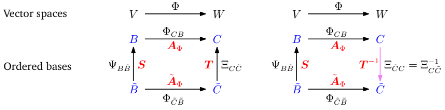
\includegraphics[width=\linewidth, height=2.5cm, keepaspectratio]{Pictures/maths/basis-change.png}
    \caption{Basis Change}
\end{figure}

\noindent\textbf{Notations}:
\begin{enumerate}
    \item linear mapping:  $\Phi : \mathbf{V \to W}$

    \item ordered bases of $\mathbf{V}$ : \(         \mathit{B} = \mathbf{(b_1, \cdots , b_n)} \quad\quad \tilde{\mathit{B}} = \mathbf{( \tilde{b}1, \cdots , \tilde{b}_n)}     \)

    \item ordered bases of $\mathbf{W}$ : \( \mathit{C} = \mathbf{(c_1, \cdots , c_n)} \quad\quad \tilde{\mathit{C}} = \mathbf{( \tilde{c}1, \cdots , \tilde{c}_n)} \)

    \item Transformation matrix of $\Phi: \mathbf{V} \to \mathbf{W}$ wrt bases $\mathit{B}$ and $\mathit{C}$ : $\mathbf{A}_\Phi \in \mathbb{R}^{m \times n}$

    \item Transformation matrix of $\Phi: \mathbf{V} \to \mathbf{W}$ wrt bases $\tilde{\mathit{B}}$ and $\tilde{\mathit{C}}$ : $\tilde{\mathbf{A}}_\Phi \in \mathbb{R}^{m \times n}$

    \item $A_\Phi$ is \textbf{transformation matrix} of $\Phi_{CB}$ wrt ordered bases $B$, $C$\\

    \item $\Psi_{B\tilde{B}} : V \to V$ maps coordinates with respect to the new basis $\tilde{B}$ onto the (unique) coordinates with respect to the “old” basis $B$ (in $V$)

    \item $\Xi_{\tilde{C}C} : W \to W$ maps coordinates with respect to $C$ onto coordinates with respect to $\tilde{C}$

    \item  \begin{align}
        \Phi_{\tilde{C}\tilde{B}}  
        &= \Xi_{\tilde{C}C} \circ \Phi_{CB} \circ \Psi_{B\tilde{B}} \\ 
        &= \Xi^{-1}_{C\tilde{C}} \circ \Phi_{CB} \circ \Psi_{B\tilde{B}} \\ 
    \end{align} 
    
\end{enumerate}

\vspace{0.2cm}
\noindent \textbf{Note}:
\begin{enumerate}
    \item Transformation matrices of a linear mapping $\Phi : \mathbf{V \to W}$ change if we change the bases in $\mathbf{V}$ and $\mathbf{W}$.

    \item 
\end{enumerate}

\begin{theorem}[Basis Change]\label{theorem: Basis Change}
    For a linear mapping $\Phi : \mathbf{V \to W}$, ordered bases\\ 
    \(
        \mathit{B} = \mathbf{(b_1, \cdots , b_n)} \quad\quad \tilde{\mathit{B}} = \mathbf{( \tilde{b}1, \cdots , \tilde{b}_n)}  \hfill \text{ of }\mathbf{V}
    \)\\
    and\\
    \(
        \mathit{C} = \mathbf{(c_1, \cdots , c_n)} \quad\quad \tilde{\mathit{C}} = \mathbf{( \tilde{c}1, \cdots , \tilde{c}_n)}  \hfill \text{ of }\mathbf{W}
    \)\\
    and a transformation matrix $\mathbf{A}_\Phi$ of $\Phi$ with respect to $\mathit{B}$ and $\mathit{C}$, the corresponding transformation matrix $\tilde{\mathbf{A}}_\Phi$ with respect to the bases $\tilde{\mathit{B}}$ and $\tilde{\mathit{C}}$ is given as\\
    \( \tilde{\mathbf{A}}_\Phi = \mathbf{T^{-\top} \mathbf{A}_\Phi S} \)
\end{theorem}

\vspace{0.2cm}
\noindent \textbf{where}:
\begin{enumerate}
    \item $\mathbf{S} \in \mathbb{R}^{n\times n}$ is the transformation matrix of $id_V$ that maps coordinates with respect to $\tilde{\mathit{B}}$ onto coordinates with respect to $\mathit{B}$

    \item $\mathbf{T} \in \mathbb{R}^{m\times m}$ is the transformation matrix of $id_W$ that maps coordinates with respect to $\tilde{\mathit{C}}$ onto coordinates with respect to $\mathit{C}$.
\end{enumerate}

\vspace{0.2cm}
\noindent \textbf{Proof}:
\begin{enumerate}
    \item we can write the vectors of the new basis $\hat{\mathit{B}}$ of $\mathbf{V}$ as a linear combination of the basis vectors of $\mathit{B}$, such that\\
    \(
        \displaystyle \hat{\mathbf{b}}_j = s_{1j}\mathbf{b}_1 + \cdots + s_{nj}\mathbf{b}_n = \sum_{i=1}^{n} s_{ij}\mathbf{b}_i \hfill (j = 1,\cdots,n)
    \)\\
    and,\\
    \(
        \displaystyle \hat{\mathbf{c}}_k = t_{1k}\mathbf{c}_1 + \cdots + t_{mk}\mathbf{c}_m = \sum_{l=1}^{n} t_{lk}\mathbf{c}_l \hfill (k = 1,\cdots,m)
    \)

    \item $\mathbf{S} = ((s_{ij})) \in \mathbb{R}^{n\times n}$ as the transformation matrix that maps coordinates with respect to $\tilde{\mathit{B}}$ onto coordinates with respect to $\mathit{B}$\\
    $j$th column of $\mathbf{S}$ is the \textbf{coordinate} representation of  $\tilde{\mathbf{b}}_j$ with respect to $\mathit{B}$\\
    $\mathbf{S}$ is a \textbf{regular matrix}.
    
    
    \item $\mathbf{T} = ((T_{lk})) \in \mathbb{R}^{m\times m}$ as the transformation matrix that maps coordinates with respect to $\tilde{\mathit{C}}$ onto coordinates with respect to $\mathit{C}$\\
    $k$th column of $\mathbf{T}$ is the \textbf{coordinate} representation of $\tilde{\mathbf{c}}_k$ with respect to $\mathbf{C}$\\
    $\mathbf{T}$ is a \textbf{regular matrix}.

    \item \( \displaystyle
        \Phi(\tilde{\mathbf{b}}_j) = \sum_{k=1}^{m} \tilde{a}_{kj}\textcolor{blue}{\tilde{\mathbf{c}}_k} = \sum_{k=1}^{m} \tilde{a}_{kj} \textcolor{blue}{\sum_{l=1}^{m} t_{lk} \mathbf{c}_l} = \sum_{l=1}^{m}\dParenBrac{ \textcolor{Magenta}{\sum_{k=1}^{m} t_{lk}\tilde{a}_{kj}} }\mathbf{c}_l
    \)  \\
    \( \displaystyle
     \Phi(\textcolor{blue}{\tilde{\mathbf{b}}_j}) = \Phi \dParenBrac{ \textcolor{blue}{\sum_{i=1}^{m} s_{ij}\mathbf{b}_i} } = \sum_{i=1}^{m} s_{ij} \textcolor{red}{\Phi(\mathbf{b}_i)} = \sum_{i=1}^{m} s_{ij} \textcolor{red}{\sum_{i=1}^{m} a_{li}\mathbf{c}_l} = \sum_{l=1}^{m}\dParenBrac{ \textcolor{Magenta}{\sum_{i=1}^{n} a_{li}s_{ij}} }\mathbf{c}_l
    \)

    \item \( \displaystyle
        \sum_{k=1}^{m} t_{lk}\tilde{a}_{kj} = \sum_{i=1}^{n} a_{li}s_{ij} 
    \)\\
    \(
        \Rightarrow \mathbf{T\tilde{A}}_\Phi = \mathbf{A}_\Phi \mathbf{S} \in \mathbb{R}^{m\times n}
    \)\\
    \(
        \Rightarrow \mathbf{\tilde{A}}_\Phi = \mathbf{T^{-\top}A}_\Phi \mathbf{S}
    \)\\
    Hence, Proved!
    
\end{enumerate}








\section{Coordinate vector/ Coordinates ( $\alpha$ ) \cite{mfml-1}}\label{Coordinate vector}\label{Coordinates}

Consider a vector space $\mathbf{V}$ and an ordered basis $\mathit{B} = \mathbf{(b_1, \cdots , b_n)}$ of $\mathbf{V}$. For any $\mathbf{x \in V}$ we obtain a unique representation (linear combination) \( \mathbf{x} = \alpha_1\mathbf{b}_1 + \cdots + \alpha_n\mathbf{b}_n \) of $\mathbf{x}$ with respect to $\mathit{B}$. Then $\alpha_1, \cdots , \alpha_n$ are the \textbf{coordinates} of $\mathbf{x}$ with respect to $\mathit{B}$, and the vector \( \displaystyle \bm{\alpha} = \begin{bmatrix} \alpha_1 & \hdots & \alpha_n \end{bmatrix}^\top \in \mathbb{R}^n \) is the \textbf{coordinate vector}/ coordinate representation of $\mathbf{x}$ with respect to the ordered basis $\mathit{B}$.


\noindent SEE:
\begin{enumerate}
    \item \fullref{ordered basis}
    \item \fullref{Linear Combination} 
\end{enumerate}

\vspace{0.2cm}
\noindent \textbf{Note}:
\begin{enumerate}
    \item For an $n$-dimensional vector space $\mathbf{V}$ and an ordered basis $\mathit{B}$ of $\mathbf{V}$, the mapping $\Phi : \mathbb{R}^n \to \mathbf{V}$, $\Phi(\mathbf{e}_i) = \mathbf{b}_i$, $i = 1, \cdots , n$, is linear (and because of \theoremref{theorem: isomorphic} an \textbf{isomorphism}), where $(\mathbf{e}_1, \cdots , \mathbf{e}_n)$ is the standard basis of $\mathbb{R}^n$.
\end{enumerate}




\section{Rank ( $rk(\mathbf{A})$ ) \cite{mfml-1}}\label{matrix: Rank}

The number of linearly independent columns of a matrix $\mathbf{A} \in \mathbb{R}^{m \times n}$ equals the number of linearly independent rows and is called the rank rank of $\mathbf{A}$ and is denoted by $rk(\mathbf{A})$.

\begin{enumerate}
    \item $rk(\mathbf{A}) = rk(\mathbf{A}^\top)$, i.e., the column rank equals the row rank.

    \item The columns of $\mathbf{A} \in \mathbb{R}^{m \times n}$ span a subspace $U \subseteq \mathbb{R}^m$ with $\dim(U) = rk(\mathbf{A})$. 

    \item The rows of $\mathbf{A} \in \mathbb{R}^{m\times n}$ span a subspace $W \subseteq \mathbb{R}^n$ with $\dim(W) = rk(\mathbf{A})$. A basis of $W$ can be found by applying Gaussian elimination to $A^\top$.

    \item For all $\mathbf{A} \in \mathbb{R}^{n\times n}$ it holds that $\mathbf{A}$ is regular (invertible) if and only if $rk(\mathbf{A}) = n$.

    \item For all $\mathbf{A} \in \mathbb{R}^{m\times n}$ and all $\mathbf{b} \in \mathbb{R}^m$ it holds that the linear equation system $\mathbf{Ax = b}$ can be solved if and only if $rk(\mathbf{A}) = rk(\mathbf{A}|\mathbf{b})$, where $\mathbf{A}|\mathbf{b}$ denotes the augmented system.

    \item For $\mathbf{A} \in \mathbb{R}^{m\times n}$ the subspace of solutions for $\mathbf{Ax = 0}$ possesses dimension $n - rk(\mathbf{A})$. This subspace is called the \textbf{kernel space}\indexlabel{kernel space} or the \textbf{null space}\indexlabel{null space}.

    \item A matrix $\mathbf{A} \in \mathbb{R}^{m\times n}$ has \textbf{full rank}\indexlabel{matrix: full rank} if its rank equals the largest possible rank for a matrix of the same dimensions. This means that the rank of a full-rank matrix is the lesser of the number of rows and columns, i.e., $rk(A) = \min(m, n)$. A matrix is said to be \textbf{rank deficient}\indexlabel{matrix: rank deficient} if it does not have full rank.

\end{enumerate}


\section{Linear Mappings/ vector space homomorphism/ linear transformation ( $\Phi(\mathbf{x})$ ) \cite{mfml-1}}\label{Linear Mappings/ vector space homomorphism/ linear transformation}

\begin{figure}[h]
    \centering
    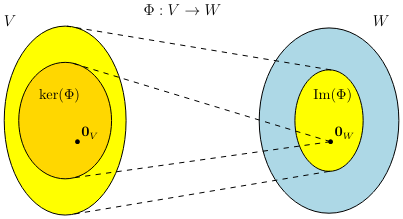
\includegraphics[width=\linewidth, height=2.5cm, keepaspectratio]{Pictures/maths/linear-mapping.png}
    \caption{Linear Mappings/ vector space homomorphism/ linear transformation}
\end{figure}

For vector spaces $V$, $W$, a mapping $\Phi : V \to W$ is called a linear mapping (or vector space homomorphism/ linear transformation) if:
\[
    \forall \mathbf{x, y} \in V, \forall\lambda, \psi \in \mathbb{R} : \Phi(\lambda\mathbf{x} + \psi\mathbf{y}) = \lambda\Phi(\mathbf{x}) + \psi\Phi(\mathbf{y})
\]

\begin{enumerate}
    \item we can represent linear mappings as matrices
    \item Consider a mapping $\Phi : \mathbb{V} \to \mathbb{W}$, where $\mathbb{V}$, $\mathbb{W}$ can be arbitrary sets. Then $\Phi$ is called
    \begin{enumerate}
        \item \textbf{Injective} if $\forall \mathbf{x, y} \in \mathbb{V}: \Phi(\mathbf{x}) = \Phi(\mathbf{y}) \Rightarrow \mathbf{x} = \mathbf{y}$ \indexlabel{Injective mapping}

        \item \textbf{Surjective} if $\Phi(\mathbb{V}) = \mathbb{W}$\indexlabel{Surjective mapping}\\
        If $\Phi$ is surjective, then every element in $\mathbb{W}$ can be “\textbf{reached}” from $\mathbb{V}$ using $\Phi$.

        \item \textbf{Bijective} if it is injective and surjective.\indexlabel{Bijective mapping}\\
        A bijective $\Phi$ can be “\textbf{undone}”, i.e., there exists a mapping $\Psi : \mathbb{W} \to \mathbb{V}$ so that $\Psi \circ \Phi(\textbf{x}) = \textbf{x}$. This mapping $\Psi$ is then called the \textbf{inverse} of $\Phi$ and normally denoted by $\Phi^{-1}$.\indexlabel{inverse linear mapping}
        
    \end{enumerate}

    \item \textbf{Isomorphism}\indexlabel{Isomorphism}: $\Phi : V \to W$ linear and bijective\\
    
    \begin{theorem}\label{theorem: isomorphic}
        Finite-dimensional vector spaces $V$ and $W$ are isomorphic if and only if $\dim(V) = \dim(W)$.
    \end{theorem}
    
    Intuitively, this means that vector spaces of the same dimension are kind of the same thing, as they can be transformed into each other without incurring any loss.\\
    This gives the justification to treat $\mathbb{R}^{m\times n}$ (the vector space of ${m\times n}$-matrices) and $\mathbb{R}^{mn}$ (the vector space of vectors of length $mn$) the same, as their dimensions are $mn$, and there exists a linear, bijective mapping that transforms one into the other.

    \item \textbf{Endomorphism}\indexlabel{Endomorphism}: $\Phi : V \to V$ linear

    \item \textbf{Automorphism}\indexlabel{Automorphism}: $\Phi : V \to V$ linear and bijective

    \item We define $id_V : V \to V , \mathbf{x} \to \mathbf{x}$ as the \textbf{identity mapping}\indexlabel{identity mapping} or \textbf{identity automorphism}\indexlabel{identity automorphism} in V.

    \item Consider vector spaces $V, W, X$. Then:
    \begin{enumerate}
        \item For linear mappings $\Phi : V \to W$ and $\Psi : W \to X$, the mapping $\Psi \circ \Phi : V \to X$ is also linear.

        \item If $\Phi : V \to W$ is an isomorphism, then $\Phi^{-1} : W \to V$ is an isomorphism, too.

        \item If $\Phi : V \to W$, $\Psi : V \to W$ are linear, then $\Phi + \Psi$ and $\lambda\Phi$, $\lambda \in \mathbb{R}$, are linear, too.
    \end{enumerate}
    
\end{enumerate}

\subsection{Matrix Representation of Linear Mappings \cite{mfml-1}}\label{Matrix Representation of Linear Mappings}

\begin{enumerate}
    \item Any $n$-dimensional vector space is \textbf{isomorphic} to $\mathbb{R}^n$. (SEE: \theoremref{theorem: isomorphic})
    
\end{enumerate}

\subsection{Transformation Matrix ( $\mathbf{A}_\Phi$ ) \cite{mfml-1}}\label{Transformation Matrix}

\begin{enumerate}
    \item Consider vector spaces $\mathbf{V}$, $\mathbf{W}$ with corresponding (ordered) bases $\mathit{B} = \mathbf{(b_1, \cdots , b_n)}$ and $\mathit{C} = \mathbf{(c_1, \cdots , c_m)}$. (SEE: \fullref{ordered basis})

    \item Moreover, we consider a linear mapping $\Phi : \mathbf{V} \to \mathbf{W}$. 

    \item For $j \in \dCurlyBrac{1, \cdots , n}$, \(     \displaystyle \Phi(\mathbf{b}_j) = \alpha_{1j}\mathbf{c}_1 + \cdots + \alpha_{mj}\mathbf{c}_m = \sum_{i=1}^{m} \alpha_{ij}\mathbf{c}_{i} \) is the \textbf{unique} representation of $\Phi(\mathbf{b}_j)$ with respect to $\mathit{C}$. 

    \item The $m \times n$-matrix $\mathbf{A}_\Phi$, whose elements are given by \( \mathbf{A}_\Phi(i, j) = \alpha_{ij} \), is called \textbf{transformation matrix} of $\Phi$ (with respect to the ordered bases $\mathit{B}$ of $\mathbf{V}$ and $\mathit{C}$ of $\mathbf{W}$)

    \item The coordinates of $\Phi(\mathbf{b}_j)$ with respect to the ordered basis $\mathit{C}$ of $\mathbf{W}$ are the $j$-th column of $\mathbf{A}_\Phi$. (SEE: \fullref{Coordinate vector})

    \item Consider (\textbf{finite-dimensional}) vector spaces $\mathbf{V, W}$ with ordered bases $\mathit{B, C}$ and a linear mapping $\Phi : \mathbf{V \to W}$ with transformation matrix $\mathbf{A}_\Phi$. \\
    If $\hat{\mathbf{x}}$ is the coordinate vector of $\mathbf{x} \in \mathbf{V}$ with respect to $\mathit{B}$ and $\hat{\mathbf{y}}$ the coordinate vector of $\mathbf{y} = \Phi(\mathbf{x}) \in \mathbf{W}$ with respect to $\mathit{C}$, then $\hat{\mathbf{y}} = \mathbf{A}_\Phi\hat{\mathbf{x}}$.

    \item The transformation matrix can be used to map coordinates with respect to an ordered basis in $\mathbf{V}$ to coordinates with respect to an ordered basis in $\mathbf{W}$.

    \item for linear mappings $\Phi : V \to W$ and $\Psi : W \to X$ the mapping $\Psi \circ \Phi : V \to X$ is also \textbf{linear}.\\
    With transformation matrices $\mathbf{A}_\Phi$ and $\mathbf{A}_\Psi$ of the corresponding mappings, the overall transformation matrix is $\mathbf{A}\Psi\circ\Phi = \mathbf{A}_\Psi \mathbf{A}_\Phi$

    \begin{enumerate}
        \item[] \fullref{Basis Change}

        \item $\mathbf{A}_\Phi$ is the transformation matrix of a linear mapping $\Phi_{CB} : V \to W$ with respect to the bases $B$, $C$.

        \item $\tilde{\mathbf{A}}_\Phi$ is the transformation matrix of the linear mapping $\tilde{\mathbf{A}}_\Phi : V \to W$ with respect to the bases $\tilde{B}, \tilde{C}$ 

        \item $\mathbf{S}$ is the \textbf{transformation matrix} of a linear mapping $\Psi_{B\tilde{B}} : V \to V$ (\textbf{automorphism}) that represents  in terms of $B$. Normally, $\Psi = id_V$ is the identity mapping in $V$

        \item $\mathbf{T}$ is the \textbf{transformation matrix} of a linear mapping $\Xi_{C\tilde{C}} : W \to W$ (\textbf{automorphism}) that represents  in terms of $C$. Normally, $\Xi = id_W$ is the identity mapping in $W$

        \item Informally, transformations just in terms of bases, then:
        \[
            \hfill
            \mathbf{A}_\Phi : B \to C
            \hfill
            \tilde{\mathbf{A}}_\Phi : \tilde{B} \to \tilde{C}
            \hfill
            \mathbf{S} : \tilde{B} \to B
            \hfill
            \mathbf{T} : \tilde{C}  \to C
            \hfill
            \mathbf{T}^{-1}: C \to \tilde{C}
            \hfill
        \]
        \[
            \hfill
            \tilde{B} \to \tilde{C}
            =
            \tilde{B} \to B \to C \to \tilde{C}
            \hfill 
            \tilde{\mathbf{A}}_\Phi = \mathbf{T}^{-1}\mathbf{A}_\Phi \mathbf{S}
            \hfill
        \]
        \[
            \hfill
            \mathbf{x} 
            \mapsto \mathbf{Sx}
            \mapsto \mathbf{A}_\Phi(\mathbf{Sx})
            \mapsto \mathbf{T}^{-1}(\mathbf{A}_\Phi(\mathbf{Sx}))
            = \mathbf{\tilde{A}}_\Phi \mathbf{x}
            \hfill
        \]

        \textbf{Note}: execution order is from right to left because vectors are multiplied at the right-hand side 
        
    \end{enumerate}
    
\end{enumerate}



%%%%%%%%%%%%%%%%%%%%%%%%%%%%%%%%%%%%%%%%%%%%%%%%%%%%%%%%%%



\section{Kernel/ null space ( $ker(\Phi)$ ) \cite{mfml-1}}\label{Kernel/ null space}

For $\Phi : V \to W$, we define the kernel/ null space 
\[
    \hfill
    ker(\Phi) := \Phi^{-1}(0_W) = \dCurlyBrac{v \in V : \Phi(v) = 0_W}
    \hfill
\]

\begin{enumerate}
    \item kernel is the set of vectors $v \in V$ that $\Phi$ maps onto the neutral element $0_W \in W$

    \item It \textbf{ALWAYS} holds that $\Phi(0_V) = 0_W$ and, therefore, $0_V \in ker(\Phi)$

    \item the null space is \textbf{NEVER} empty

    \item $ker(\Phi) \subseteq V$ is a subspace of $V$

    
\end{enumerate}


%%%%%%%%%%%%%%%%%%%%%%%%%%%%%%%%%%%%%%%%%%%%%%%%%%%%%%%%%%


\section{Image/ range ( $Im(\Phi)$ ) \cite{mfml-1}}\label{Image/ range}

For $\Phi : V \to W$, we define the image/ range 
\[
    \hfill
    Im(\Phi) := \Phi(V) = \dCurlyBrac{w \in W | \exists v \in V : \Phi(v) = w}
    \hfill
\]

\begin{enumerate}
    \item image is the set of vectors $w \in W$ that can be “reached” by $\Phi$ from any vector in $V$

    \item $Im(\Phi) \subseteq W$ is a subspace of $W$
\end{enumerate}



%%%%%%%%%%%%%%%%%%%%%%%%%%%%%%%%%%%%%%%%%%%%%%%%%%%%%%%%%%

\section{Domain and Codomain \cite{mfml-1}}\label{Domain and Codomain}

if $\Phi : V \to W$, then:
\begin{enumerate}
    \item $V$ is domain
    \item $W$ is codomain
\end{enumerate}

%%%%%%%%%%%%%%%%%%%%%%%%%%%%%%%%%%%%%%%%%%%%%%%%%%%%%%%%%%

\section{Null Space and Column Space \cite{mfml-1}}\label{Null Space and Column Space}

Let us consider $\mathbf{A} \in \mathbb{R}^{m\times n}$ and a linear mapping $\Phi : \mathbb{R}^n \to \mathbb{R}^m$, $\mathbf{x} \mapsto \mathbf{Ax}$.

\begin{enumerate}
    \item For $\mathbf{A} = [\mathbf{a}_1, \cdots , \mathbf{a}_n]$, where $\mathbf{a}_i$ are the columns of $\mathbf{A}$:
    \begin{align*}
        \displaystyle
        Im(\Phi) 
        &= \dCurlyBrac{ \mathbf{Ax} : \mathbf{x} \in \mathbb{R}^n } \\
        &= \dCurlyBrac{ \sum_{i=1}^{n} x_i\mathbf{a}_i : \forall x_i \in \mathbb{R}, i=1,\cdots,n } \\
        &= span[\mathbf{a}_1,\cdots, \mathbf{a}_n] \subseteq \mathbb{R}^m \\
    \end{align*}

    the image is the span of the columns of A, also called the \textbf{column space}\indexlabel{column space}. Therefore, the column space (image) is a subspace of $\mathbb{R}^m$, where m is the \textbf{“height” of the matrix}\indexlabel{height of the matrix}.

    \item $rk(\mathbf{A}) = dim(Im(\Phi))$

    \item The kernel/null space $ker(\Phi)$ is the general solution to the homogeneous system of linear equations $\mathbf{Ax = 0}$ and captures all possible linear combinations of the elements in $\mathbb{R}^n$ that produce $\mathbf{0} \in \mathbb{R}^m$.

    \item The kernel is a subspace of $\mathbb{R}^n$, where $n$ is the \textbf{“width” of the matrix}\indexlabel{width of the matrix}.

    \item The kernel focuses on the relationship among the columns, and we can use it to determine whether/ how we can express a column as a linear combination of other columns.
\end{enumerate}



%%%%%%%%%%%%%%%%%%%%%%%%%%%%%%%%%%%%%%%%%%%%%%%%%%%%%%%%%%


\section{Rank-Nullity Theorem ( $dim(ker(\Phi)) + dim(Im(\Phi)) = dim(V)$ ) \cite{mfml-1}}\label{Rank-Nullity Theorem}

For vector spaces $V, W$ and a linear mapping $\Phi : V \to W$ it holds that 

\[
    \hfill
    dim(ker(\Phi)) + dim(Im(\Phi)) = dim(V)
    \hfill
\]

The rank-nullity theorem is also referred to as the \textbf{fundamental theorem of linear mappings}\indexlabel{fundamental theorem of linear mappings}.

\begin{enumerate}
    \item If $dim(Im(\Phi)) < dim(V)$, then $ker(\Phi)$ is non-trivial, i.e., the kernel contains more than $0_V$ and $dim(ker(\Phi)) \geq 1$

    \item If $\mathbf{A}_\Phi$ is the transformation matrix of $\Phi$ with respect to an ordered basis and $dim(Im(\Phi)) < dim(V)$, then the system of linear equations $\mathbf{A}_\Phi x = 0$ has infinitely many solutions

    \item If $dim(V) = dim(W)$, then the following three-way equivalence holds: 
    \begin{enumerate}
        \item $\Phi$ is injective

        \item $\Phi$ is surjective

        \item $\Phi$ is bijective 
    \end{enumerate}
    since $Im(\Phi) \subseteq W$

    
\end{enumerate}



%%%%%%%%%%%%%%%%%%%%%%%%%%%%%%%%%%%%%%%%%%%%%%%%%%%%%%%%%%



\section{Affine Subspace/ linear manifold ( $L = x0 + U$ ) \cite{mfml-1}}\label{Affine Subspace/ linear manifold}

Let $V$ be a vector space, $x_0 \in V$ and $U \subseteq V$ a subspace. Then the subset

\begin{table}[h]
    \begin{minipage}{0.49\linewidth}
        \begin{align*}
            L &= x_0 + U\\
             &= \dCurlyBrac{x_0 + u : u \in U} \\
             &= \dCurlyBrac{v \in V | \exists u \in U : v = x_0 + u} \subseteq V
        \end{align*}
    \end{minipage}
    \hfill
    \begin{minipage}{0.49\linewidth}
        \begin{table}[H]
            \begin{tabular}{l l}
                $U$ & direction or direction space \\
                $x_0$ & support point \\
            \end{tabular}
        \end{table}
    \end{minipage}
\end{table}

is called affine subspace or linear manifold of $V$. 


\begin{enumerate}
    \item an affine subspace is not a (linear) subspace (vector subspace) of $V$ for $x_0 \not\in U$

    \item Consider two affine subspaces $L = x_0 + U$ and  of a vector space $V$\\
    $L \subseteq \tilde{L}$ if and only if $U \subseteq \tilde{U}$ and $x_0 - \tilde{x}_0 \in \tilde{U}$
    
    \item Describing affine space using parameters:
    \begin{enumerate}
        \item Consider a k-dimensional affine space $L = x_0 + U$ of $V$

        \item If $\mathbf{(b_1, \cdots , b_k)}$ is an ordered basis of $U$, then every element $x \in L$ can be uniquely described as
        \[
            \hfill 
            x = x_0 + \lambda_1b_1 + \cdots + \lambda_kb_k 
            \hfill
        \]
        where $\lambda_1, \cdots , \lambda_k \in \mathbb{R}$

        \item This representation is called \textbf{parametric equation}\indexlabel{parametric equation} of $L$ with directional vectors $b_1, \cdots , b_k$ and parameters $\lambda_1, \cdots , \lambda_k$
        
    \end{enumerate}
    
\end{enumerate}


%%%%%%%%%%%%%%%%%%%%%%%%%%%%%%%%%%%%%%%%%%%%%%%%%%%%%%%%%%


\section{System of Linear Equations \cite{mfml-1}}\label{System of Linear Equations}

\subsection*{Setup/ Scenario}

\textbf{Equations}:

\noindent\textbf{Common/ Classical representation}:
\[
    \begin{matrix}
        a_{11}x_1 + a_{12}x_2 + \cdots + a_{1n}x_n = b_1\\
        \vdots \\
        a_{m1}x_1 + a_{m2}x_2 + \cdots + a_{mn}x_n = b_m
    \end{matrix}
\]       
\textbf{Matrix-vector representations/ Compact representations} ( $Ax=b$ ):
\[
    \begin{bmatrix}
        a_{11}\\ \vdots\\ a_{m1}
    \end{bmatrix} x_1 +
    \begin{bmatrix}
        a_{12}\\ \vdots\\ a_{m2}
    \end{bmatrix} x_2 +
    \cdots
    \begin{bmatrix}
        a_{1n}\\ \vdots\\ a_{mn}
    \end{bmatrix} x_n
    =
    \underset{A}{
        \underbrace{
            \begin{bmatrix}
                a_{11} & \cdots & a_{1n}\\
                \vdots & \ddots & \vdots \\
                a_{m1} & \cdots & a_{mn}\\
            \end{bmatrix}
        }
    }
    \underset{x}{
        \underbrace{
            \begin{bmatrix}
                x_1 \\ \vdots \\ x_n
            \end{bmatrix}
        }
    }
    =
    \underset{b}{
        \underbrace{
            \begin{bmatrix}
                b_{1}\\ \vdots\\ b_{m}
            \end{bmatrix}
        }
    }
\]


\begin{table}[h]
    \begin{tabular}{l l l}
        no of \textbf{equations} & $m$ & $(i=1,\cdots,m)$\\
        no of \textbf{variables} & $n$ & $(j=1,\cdots,n)$ \\
        \textbf{unknowns} & $x = (x_1,\cdots,x_n) \in R^n$\\
        \textbf{knowns} & $a_{ij}, b_{i} \in R$
    \end{tabular}
\end{table}


\subsection{Homogeneous systems of linear equations ( $\mathbf{Ax = 0}$ ) \cite{mfml-1, chatgpt}}\label{Homogeneous systems of linear equations}

\begin{enumerate}
    \item For homogeneous equation systems $\mathbf{Ax = 0}$ the solution was a vector subspace, which we can also think of as a special affine space with support point $\mathbf{x}_0 = \mathbf{0}$.

    \item A homogeneous system of linear equations is one in which \textbf{ALL} the constant terms are zero.
\end{enumerate}

\vspace{0.2cm}
\textbf{Properties}:
\begin{enumerate}
    \item \textbf{Trivial Solution}: The system always has at least one solution, the trivial solution $\mathbf{x}=0$.

    \item \textbf{Non-Trivial Solutions}: If the number of equations is less than the number of unknowns ($m<n$), there are typically an infinite number of solutions. This occurs because the system is underdetermined.

    \item \textbf{Solution Space}: The solutions form a subspace of $\mathbb{R}^n$, specifically the null space of the matrix $\mathbf{A}$.
\end{enumerate}



\subsection{Inhomogeneous systems of linear equations ( $\mathbf{Ax = b}$ ) \cite{mfml-1, chatgpt}}\label{Inhomogeneous systems of linear equations}


\begin{enumerate}
    \item For $\mathbf{A} \in \mathbb{R}^{m\times n}$ and $\mathbf{x} \in \mathbb{R}^m$, the solution of the system of linear equations $\mathbf{A\boldsymbol{\lambda} = x}$ is either the empty set or an affine subspace of Rn of dimension $n - rk(\mathbf{A})$.

    \item The solution of the linear equation $\lambda_1\mathbf{b}_1 + \cdots + \lambda_n\mathbf{b}_n = \mathbf{x}$, where $(\lambda_1, \cdots , \lambda_n) \neq (0, \cdots , 0)$, is a hyperplane in $\mathbb{R}^n$.

    \item In $\mathbb{R}^n$, every $k$-dimensional affine subspace is the solution of an inhomogeneous system of linear equations $\mathbf{Ax = b}$, where $\mathbf{A} \in \mathbb{R}^{m\times n}$, $\mathbf{b} \in \mathbb{R}^m$ and $rk(\mathbf{A}) = n - k$.

    \item An inhomogeneous system of linear equations includes non-zero constant terms.
\end{enumerate}

\vspace{0.2cm}
\textbf{Properties}:
\begin{enumerate}
    \item \textbf{Existence of Solutions}: Solutions exist if and only if the vector $\mathbf{b}$ lies in the column space of $\mathbf{A}$. This is determined by checking if the system $\mathbf{[A|b]}$ is consistent (i.e., there are no contradictions in the augmented matrix).

    \item \textbf{Uniqueness of Solutions}: If the matrix $\mathbf{A}$ has full column rank and $m=n$ (i.e., the matrix is square and invertible), the system has a unique solution. If A does not have full column rank, the system may have no solutions or infinitely many solutions.

    \item \textbf{Particular and General Solutions}: If a particular solution $\mathbf{x}_p$ exists, the general solution can be written as $\mathbf{x}=\mathbf{x}_p +\mathbf{x}_h$, where $\mathbf{x}_h$ is the general solution to the corresponding homogeneous system $\mathbf{Ax=0}$.
\end{enumerate}

\subsection{Consistent System}\label{Consistent System of equations}

\begin{enumerate}
    \item A system of equations is considered consistent if there exists \textbf{AT LEAST ONE SOLUTION} that satisfies all the equations.
\end{enumerate}


\subsection{Dependent Solution}\label{Dependent Solution of linear equations}

\begin{enumerate}
    \item happens when no of equations $<$ no of variables
    
    \item Solutions are dependent if one can be expressed as a linear combination of the others.
\end{enumerate}

\subsection{Types of Solutions}
\begin{enumerate}
    \item \textbf{No solution}
    \begin{enumerate}
        \item Inconsistent
    \end{enumerate}
    
    \item \textbf{Unique solution}
    \begin{enumerate}
        \item Consistent
        \item Independent
    \end{enumerate}

    \item \textbf{Infinitely many solutions}
    \begin{enumerate}
        \item Consistent
        \item Dependent
    \end{enumerate}

    \item \textbf{Trivial solution}
    \begin{enumerate}
        \item $x_i = 0, \forall x_i$, is a solution
        \item Consistent
        \item Dependent
    \end{enumerate}

\end{enumerate}


\subsection{Elementary Transformations \cite{mfml-1}} \label{Elementary Transformations}
transformations that keep the solution set the same, but that transform the equation system into a simpler form:
\begin{enumerate}
    \item Exchange of two equations (rows in the matrix representing the system of equations)
    \[ R_i \Leftrightarrow R_j \]

    \item Multiplication of an equation (row) with a constant $\lambda \in R\backslash \dCurlyBrac{0}$
    \[ R_i := \lambda R_i \]

    \item Addition of two equations (rows)
    \[ R_i := R_i + R_j \]

\end{enumerate}


\subsection{Solutions of system of linear equations \cite{mfml-1}}\label{Solutions of system of linear equations}

\begin{table}[h]
    \begin{tabular}{l l}
        Original System	& $Ax = b$ \\

        Homogeneous System & $Ax = 0$ \\
    \end{tabular}
\end{table}

\begin{align*}
   & Ax = b \\
   & \Rightarrow A(x_0 + \lambda _1x_1 + \lambda _2x_2 + \cdots ) = b	&&& (\lambda _i \in R) \\
   & \Rightarrow Ax_0 + \lambda _1Ax_1 + \lambda _2Ax_2 + \cdots  = b + 0 + 0 + \cdots  = b
\end{align*}

\begin{table}[h]
    \begin{tabular}{l l l}
        $x = x0$ & particular solution & ($Ax = b$ part) \\
        
        $x = x_1, x_2, \cdots$ & solutions to homogeneous equation & ($Ax = 0$ part)
    \end{tabular}
\end{table}

\subsubsection{Augmented Matrix ( $[A|b]$ ) \cite{mfml-1}} \label{Augmented Matrix}

An augmented matrix for a system of equations is a matrix of numbers in which each row represents the constants from one equation (both the coefficients and the constant on the other side of the equal sign) and each column represents all the coefficients for a single variable.


\subsubsection{Row-Echelon Form (REF) \cite{mfml-1,wiki/Row_echelon_form}}\label{Row-Echelon Form (REF)}

\begin{enumerate}
    \item A matrix is in row echelon form if it can be obtained as the result of \textbf{Gaussian elimination}.

    \item Every matrix can be put in row echelon form by applying a sequence of \textbf{elementary row operations}.

    \item can be viewed as a generalization of \textbf{upper triangular} form for rectangular matrices

    \item pivots may not be $1$
\end{enumerate}


\subsubsection{Reduced Row Echelon Form (RREF) \cite{mfml-1,wiki/Row_echelon_form}}\label{Reduced Row Echelon Form (RREF)}
A matrix is in row-echelon form if:
\begin{enumerate}
    \item All rows that contain only zeros are at the bottom of the matrix; correspondingly, all rows that contain at least one nonzero element are on top of rows that contain only zeros.

    \item Looking at nonzero rows only, the first nonzero number from the left (also called the pivot or the leading coefficient) is always strictly to the right of the pivot of the row above it.
\end{enumerate}

\noindent\textbf{Note}:
\begin{enumerate}
    \item A matrix is in row echelon form if it can be obtained as the result of \textbf{Gauss–Jordan elimination}

    \item it is in row echelon form, with the additional property that the first nonzero entry of each row is equal to $1$ and is the only nonzero entry of its column

    \item The reduced row echelon form of a matrix is \textbf{unique} and does not depend on the sequence of elementary row operations used to obtain it

    \item pivots \textbf{MUST} be $1$
\end{enumerate}

\subsubsection{Particular Solution (or special solution) \cite{mfml-1}} \label{Particular Solution (or special solution)}
solution of $Ax = b$

\paragraph{Direct Solution  \cite{mfml-1}}

\textbf{Conditions}:
\begin{enumerate}
    \item A is a \textbf{square matrix} and \textbf{invertible}
\end{enumerate}

\[ Ax = b \Leftrightarrow x = A^{-1}b \]

\textbf{Disadvantage}:
\begin{enumerate}
    \item not good at numerical precision
\end{enumerate}


\paragraph{Pseudo Direct Solution \cite{mfml-1}}
\textbf{Conditions}:
\begin{enumerate}
    \item $A$ needs to have \textbf{linearly independent columns}
\end{enumerate}

\[
    Ax = b 
    \Leftrightarrow 
    A^\top Ax = A^\top b 
    \Leftrightarrow
    x = (A^\top A)^{-1}A^\top b
\]

\textbf{Disadvantage:}
\begin{enumerate}
    \item requires many computations for the matrix-matrix product and computing the inverse of $A^\top A$

    \item not good at numerical precision
\end{enumerate}



\paragraph{Using Gaussian Elimination}
\textbf{Steps:}
\begin{enumerate}
    \item use RREF on Augmented matrix $[A|b]$

    \item express the right-hand side of the equation system using the pivot columns, such that ${\displaystyle b = \sum_{i=1}^{P} \lambda_i p_i}$ where $p_i$ are pivot columns.

    \item $\lambda _i$ are determined easiest if we start with the rightmost pivot column and work our way to the left

    \item solution = $x_0 = [\lambda _1, \lambda _2, \cdots, \lambda _P]^\top$
\end{enumerate}

\subsubsection{Solutions of $Ax=0$ \cite{mfml-1}}

Every subspace $U \subseteq (R^n , +, \cdot)$ is the solution space of a homogeneous system of linear equations $Ax = 0$ for $x \in R^n$
\begin{enumerate}
    \item As it is a homogeneous system, there can’t be “No Solution”

    \item Solutions will be:
    \begin{enumerate}
        \item Unique solution (trivial) = $0^n \in R^n$
        \item infinite solutions
    \end{enumerate}
\end{enumerate}


\paragraph{The Minus-$1$ Trick \cite{mfml-1}}\label{Solutions of ax=0: The Minus-1 Trick}
\textbf{Steps}:
\begin{enumerate}
    \item $A := RREF(A)$

    \item ignore the rows with only 0s
    \[
        A = 
        \begin{bmatrix}
            0 & \cdots  & 0 & 1 & \ast & \cdots  & \ast & 0 & \ast & \cdots  & \ast & 0 & \ast & \cdots  & \ast\\
            \vdots && \vdots & 0 & 0 & \cdots  & 0 & 1 & \ast & \cdots  & \ast & \vdots & \vdots & & \vdots\\
            \vdots & & \vdots & \vdots & \vdots & & \vdots & 0 & \vdots & & \vdots & \vdots & \vdots && \vdots\\
            \vdots & & \vdots & \vdots & \vdots & & \vdots & \vdots & \vdots & & \vdots & 0 & \vdots && \vdots\\
            0 & \cdots & 0 & 0 & 0 & \cdots & 0 & 0 & 0 & \cdots & 0 & 1 & \ast & \cdots & \ast\\
        \end{bmatrix}
    \]
    where $\ast$ can be an arbitrary real number, with the constraints that the \textbf{first nonzero entry} per row must be $1$ and all other entries in the corresponding column must be $0$. 

    \item columns $j_1, \cdots , j_k$ with the pivots are the standard unit vectors $e_1, \cdots , e_k \in R^k$

    \item extend this matrix to an $n \times n$-matrix $B$ by adding $n - k$ rows of the form
    \[
        \begin{bmatrix}
            0 & \cdots & 0 & -1 & 0 & \cdots & 0
        \end{bmatrix}
    \]
    so that the \textbf{diagonal} of the augmented matrix $B$ contains either $1$ or $-1$

    \item columns of $B$ that contain the $-1$ as pivots are solutions of the homogeneous equation system $Ax = 0$

\end{enumerate}

\paragraph{Classical method \cite{mfml-1}}\label{Solutions of ax=0: Classical method}

\textbf{Steps}:
\begin{enumerate}
    \item $A := RREF(A)$

    \item express the pivot variables in terms of free variables

    \item for each free variable, put it $1$ and rest free variables as $0$s

    \item get $n-k$ solutions

\end{enumerate}


\subsubsection{General Solution to $Ax=b$ \cite{mfml-1}}\label{General Solution to Ax=b}

General Solution = Particular Solution (solution of $Ax=b$) + $\lambda_i$ * (solutions of $Ax = 0$)


\subsection{Systems of linear equations and affine subspaces \cite{mfml-1}}\label{Systems of linear equations and affine subspaces}
\begin{enumerate}
    \item For $A \in  R^{m\times n}$ and $x \in  R^m$, the solution of the system of linear equations $A\lambda  = x$ is either the empty set or an affine subspace of $Rn$ of dimension $n - rk(A)$. 

    \begin{enumerate}
        \item In particular, the solution of the linear equation $\lambda _1b_1 + \cdots  + \lambda _nb_n = x$, where $(\lambda _1, \cdots  , \lambda _n) \neq (0, \cdots  , 0)$, is a hyperplane in $R^n$
    \end{enumerate}

    \item In $R^n$, \textbf{EVERY} $k$-dimensional affine subspace is the solution of an inhomogeneous system of linear equations $Ax = b$, where $A \in  R^{m\times n}$, $b \in  R^m$ and $rk(A) = n - k$

    \item for homogeneous equation systems $Ax = 0$ the solution was a vector subspace, which we can also think of as a special affine space with support point $x0 = 0$
\end{enumerate}




%%%%%%%%%%%%%%%%%%%%%%%%%%%%%%%%%%%%%%%%%%%%%%%%%%%%%%%%%%%


\section{Affine Mapping \cite{mfml-1}}\label{Affine Mapping}

For two vector spaces $V, W$, a linear mapping $\Phi : V \to W$, and $\mathbf{a} \in W$, the mapping

\[
    \hfill
    \phi : V \to W
    \hfill
    \mathbf{x} \mapsto \mathbf{a} + \Phi(\mathbf{x})
    \hfill
\]

is an affine mapping from $V$ to $W$. The vector $\mathbf{a}$ is called the \textbf{translation vector}\indexlabel{affine mapping: translation vector} of $\phi$.

\begin{enumerate}
    \item Every affine mapping $\phi : V \to W$ is also the composition of a linear mapping $\Phi : V \to W$ and a translation $\tau : W \to W$ in $W$, such that $\phi = \tau \circ \Phi$. The mappings $\Phi$ and $\tau$ are uniquely determined.

    \item The composition $\phi' \circ \phi$ of affine mappings $\phi : V \to W$, $\phi': W \to X$ is affine.

    \item Affine mappings keep the geometric structure invariant. 
    
    \item They also preserve the dimension and parallelism.
\end{enumerate}


\section{Bilinear mapping ( $\Omega$ )}\label{Bilinear mapping}

Let $V$ be a vector space and $\Omega  : V × V \to R$ be a bilinear mapping that takes two vectors and maps them onto a real number. Then
\begin{enumerate}
    \item $\Omega$  is called symmetric if $\Omega (x, y) = \Omega (y, x)$ for all $x, y \in  V$ , i.e., the order of the arguments does not matter

    \item $\Omega$  is called positive definite if $\forall x \in  V\backslash \dCurlyBrac{0} : \Omega (x, x) > 0 , \Omega (0, 0) = 0$
\end{enumerate}

\vspace{0.2cm}
A bilinear mapping $\Omega $ is a mapping with two arguments, and it is linear in each argument, i.e., when we look at a vector space $V$ then it holds that for all $x, y, z \in V, \lambda , \Psi \in R$ that:
\begin{enumerate}
    \item $\Omega (\lambda x + \Psi y, z) = \lambda \Omega (x, z) + \Psi\Omega (y, z)$
    \item $\Omega (x, \lambda y + \Psi z) = \lambda \Omega (x, y) + \Psi\Omega (x, z)$
\end{enumerate}



\section{Rotation ( $\Phi$ ) \& Rotation Matrix ($R(\theta )$ ) \cite{mfml-1}}\label{Rotation and Rotation Matrix}

\begin{enumerate}
    \item A rotation is a linear mapping (more specifically, an automorphism of a \textbf{Euclidean vector space}\indexlabel{Euclidean vector space}) that rotates a plane by an angle $\theta$  about the origin, i.e.,the origin is a fixed point. 

    \item For a positive angle $\theta  > 0$, by common convention, we rotate in a \textbf{counter-clockwise direction}.

    \item Rotations $\Phi$  are linear mappings so that we can express them by a \textbf{rotation matrix} $R(\theta )$

    \item rotation performs a \textbf{basis change}
\end{enumerate}

\subsection{Rotation in $2$-D $R^2$ \cite{mfml-1}}\label{Rotation in 2-D}

\begin{enumerate}
    \item Rotation about a point (origin $[0, 0]^\top$)
    \[
        \hfill
        \Phi(e_1) =
        \begin{bmatrix}
            cos(\theta) \\ 
            sin(\theta)
        \end{bmatrix}
        \hfill
        \Phi(e_2) =
        \begin{bmatrix}
            -sin(\theta)\\
            cos(\theta)  
        \end{bmatrix}
        \hfill
    \]
    \[
        \hfill
        R(\theta) = 
        \begin{bmatrix}
            \Phi(e_1) & \Phi(e_2)
        \end{bmatrix} =
        \begin{bmatrix}
            cos(\theta) & -sin(\theta)\\ 
            sin(\theta) & cos(\theta)
        \end{bmatrix}
        \hfill
    \]
\end{enumerate}


\subsection{Rotation in $3$-D $R3$ \cite{mfml-1}} \label{Rotation in 3-D}

\begin{enumerate}
    \item Rotation about a $1$-d axis:
    \begin{enumerate}
        \item Rotation about the $e_1$-axis:
        \[
            R_1(\theta) =
            \begin{bmatrix}
                \Phi(e_1) & \Phi(e_2) & \Phi(e_3)
            \end{bmatrix} =
            \begin{bmatrix}
                1 & 0 & 0\\
                0 & cos(\theta) & -sin(\theta) \\
                0 & sin(\theta) & cos(\theta)
            \end{bmatrix}
        \]

        \item Rotation about the $e_2$-axis:
        \[
            R_2(\theta) =
            \begin{bmatrix}
                cos(\theta) & 0 & sin(\theta) \\
                0 & 1 & 0\\
                -sin(\theta) & 0 & cos(\theta)
            \end{bmatrix}
        \]

        \item Rotation about the $e_3$-axis:
        \[
            R_3(\theta) =
            \begin{bmatrix}
                cos(\theta) & -sin(\theta) & 0 \\
                sin(\theta) & cos(\theta) & 0 \\
                0 & 0 & 1 \\
            \end{bmatrix}
        \]
    \end{enumerate}

\end{enumerate}


\subsection{Givens Rotation (Rotation in $n$-D) $R^n$}\label{Givens Rotation (Rotation in n-D)}

Let $V$ be an $n$-dimensional Euclidean vector space and $\Phi : V \to V$ an automorphism with transformation matrix:

\[
    R_{ij}(\theta) :=
    \begin{bmatrix}
        I_{i-1} & 0 & \cdots & \cdots & 0\\
        0 & cos(\theta) & 0 & -sin(\theta) & 0 \\
        0 & 0 & I_{j-i-1} & 0 & 0 \\
        0 & sin(\theta) & 0 & cos(\theta) & 0 \\
        0 & \cdots & \cdots & 0 & I_{n-j} \\
    \end{bmatrix} \in R^{n\times n}
    \hfill
    (1 \leq i < j \leq n \text{ and } \theta  \in R)
\]

$R_{ij}(\theta )$ is the identity matrix In with:
\[
    \hfill
    r_{ii} = cos(\theta )
    \hfill
    r_{ij} = -sin(\theta )
    \hfill
    r_{ji} = sin(\theta )
    \hfill
    r_{jj} = cos(\theta )
    \hfill
\]


\begin{enumerate}
    \item for $2$-D ($n=2$), its a special case
\end{enumerate}

\noindent
\textbf{Properties}:
\begin{enumerate}
    \item Rotations preserve distances, i.e., $\dnorm{x-y} = \dnorm{R_\theta (x) - R_\theta (y)}$

    \item rotations leave the distance between any two points unchanged after the transformation

    \item Rotations preserve angles, i.e., the angle between $R_\theta x$ and $R_\theta y$ equals the angle between $x$ and $y$

    \item Rotations in three (or more) dimensions are generally not commutative. Therefore, the order in which rotations are applied is important, even if they rotate about the same point. 

    \item Only in two dimensions vector rotations are commutative, such that 
    \[
        R(\phi)R(\theta ) = R(\theta )R(\phi)
        \hfill
        (\phi, \theta  \in [0, 2\pi))
    \]

    \item They form an Abelian group (with multiplication) only if they rotate about the same point (e.g., the origin)

\end{enumerate}





\vspace{4cm}
\url{https://drive.google.com/file/d/1JS4tlbMRYv8oHYrLgISR_NV9y6-_2j5h/edit}\\
76 / 417












































































































































































    \chapter{Matrix \cite{mfml-1}}\label{chapter: Matrix}

\section*{Intro \cite{mfml-1}}

With $m, n \in \mathbb{N}$ a real-valued $(m, n)$-matrix $\mathbf{A}$ is an $m\cdot n$-tuple of elements $a_{ij}$, $i = 1, \cdots , m$, $j = 1, \cdots , n$, which is ordered according to a rectangular scheme consisting of $m$ rows and $n$ columns:
\[
    \hfill
    \mathbf{A} = \begin{bmatrix}
        a_{11} & a_{12} & \cdots & a_{1n}\\
        a_{21} & a_{22} & \cdots & a_{2n}\\
        \vdots & \vdots & \ddots & \vdots\\
        a_{m1} & a_{m2} & \cdots & a_{mn}\\
    \end{bmatrix}
    \in \mathbb{R}^{m\times n}
    \hfill
\]

\begin{enumerate}
    \item $\mathbb{R}^{m\times n}$ is the set of all real-valued $(m, n)$-matrices

    \item (\textbf{flattening}) $\mathbf{A} \in \mathbb{R}^{m\times n}$ (matrix) can be equivalently represented as $\mathbf{a} \in \mathbb{R}^{mn\times 1}$ (vector) by stacking all $n$ columns of the matrix into a long vector
\end{enumerate}


\section{Matrix Addition ( $\mathbf{A + B}$ ) \cite{mfml-1}}\label{Matrix Addition}
The sum of two matrices $\mathbf{A, B} \in \mathbb{R}^{m\times n}$ is defined as the element-wise sum:
\[
    \hfill
    \mathbf{A + B} = \begin{bmatrix}
        a_{11} + b_{11} & a_{12} + b_{12} & \cdots & a_{1n} + b_{1n}\\
        a_{21} + b_{21} & a_{22} + b_{22} & \cdots & a_{2n} + b_{2n}\\
        \vdots & \vdots & \ddots & \vdots\\
        a_{m1} + b_{m1} & a_{m2} + b_{m2} & \cdots & a_{mn} + b_{mn}\\
    \end{bmatrix}
    \in \mathbb{R}^{m\times n}
    \hfill
\]


\section{Matrix Multiplication ( $AB = A@B$ ) \cite{mfml-1}}
For matrices $\mathbf{A} \in \mathbb{R}^{m\times n}$, $\mathbf{B} \in \mathbb{R}^{n\times k}$, the elements $c_{ij}$ of the product $C = AB = A@B \in \mathbb{R}^{m\times k}$ are computed as:
\[
    \displaystyle
    c_{ij} = \sum_{n}^{l=1} a_{il}b_{lj}
    \hfill
    (i=1,\cdots,m)(j=1,\cdots,k)
\]

\begin{enumerate}
    \item to compute element $c_{ij}$ we multiply the elements of the $i$th row of $\mathbf{A}$ with the $j$th column of $\mathbf{B}$ and sum them up

    \item Matrices can only be multiplied if their “neighboring” dimensions match

    \item Matrix multiplication is \textbf{NOT} defined as an element-wise operation on matrix elements, i.e., $c_{ij} \neq a_{ij}b_{ij}$

    \item matrix multiplication is \textbf{NOT} commutative, i.e., $\mathbf{AB \neq BA}$
\end{enumerate}


\section{Equivalence ( $\mathbf{\tilde{A} = T^{-1}AS}$ ) \cite{mfml-1}}\label{Equivalence}

Two matrices $\mathbf{A, \tilde{A}} \in \mathbb{R}^{m\times n}$ are equivalent if there exist regular matrices $\mathbf{S} \in \mathbb{R}^{n\times n}$ and $\mathbf{T} \in \mathbb{R}^{m\times m}$, such that $\mathbf{\tilde{A} = T^{-1}AS}$.

\begin{enumerate}
    \item equivalent matrices are \textbf{NOT} necessarily similar.
\end{enumerate}


\section{Similarity/ Similar Matrices ( $\mathbf{\tilde{A} = S^{-1}AS}$ ) \cite{mfml-1}}\label{Similarity/ Similar Matrices}

Two matrices $\mathbf{A, \tilde{A}} \in \mathbb{R}^{m\times n}$ are similar if there exists a regular matrix $\mathbf{S} \in \mathbb{R}^{n\times n}$ with $\mathbf{\tilde{A} = S^{-1}AS}$.

\begin{enumerate}
    \item Similar matrices are \textbf{ALWAYS} equivalent.
\end{enumerate}


\section{Hadamard Product/ element-wise product ( $A \odot B$ )}\label{matrix: Hadamard Product/ element-wise product}

For matrices $\mathbf{A, B} \in \mathbb{R}^{m\times n}$, the elements $c_{ij}$ of the product $C \in \mathbb{R}^{m\times n}$ are computed as:
\[
    \hfill
    C = A \odot B 
    \Rightarrow c_{ij} = a_{ij}b_{ij}
    \hfill
\]


\section{Special matrices}

\subsection{Identity Matrix ( $\mathbf{I}_n \in \mathbb{R}^{n\times n}$ ) \cite{mfml-1}}\label{Identity Matrix}
In $\mathbb{R}^{n\times n}$, we define the identity matrix:
\[
    \renewcommand{\arraystretch}{0.6}
    \mathbf{I}_n = \begin{bmatrix}
        1 & 0 & \cdots & 0 & \cdots & 0 \\
        0 & 1 & \cdots & 0 & \cdots & 0 \\
        \vdots & \vdots & \ddots & \vdots & \ddots & \vdots \\
        0 & 0 & \cdots & 1 & \cdots & 0 \\
        \vdots & \vdots & \ddots & \vdots & \ddots & \vdots \\
        0 & 0 & \cdots & 0 & \cdots & 1 \\
    \end{bmatrix} \in \mathbb{R}^{n\times n}
\]

%%%%%%%%%%%%%%%%%%%%%%%%%%%%%%%%%%%%%%%%%%%%%%%%%%%%%%%%%%%%%

\section{Square Matrix ( $\mathbf{A} \in \mathbb{R}^{n\times n}$ ) \cite{mfml-1}}\label{Square Matrix}
\begin{enumerate}
    \item possesses the same number of columns and rows
\end{enumerate}

%%%%%%%%%%%%%%%%%%%%%%%%%%%%%%%%%%

\subsection{Diagonal Matrix ( $\mathbf{D} \in \mathbb{R}^{n\times n}$ ) \cite{mfml-1}}\label{Diagonal Matrix}

A diagonal matrix is a matrix that has value zero on all off-diagonal elements, i.e., they are of the form:
\[
    \renewcommand{\arraystretch}{0.6}
    \mathbf{D} = \begin{bmatrix}
        c_1 & 0 & \cdots & 0 & \cdots & 0 \\
        0 & c_2 & \cdots & 0 & \cdots & 0 \\
        \vdots & \vdots & \ddots & \vdots & \ddots & \vdots \\
        0 & 0 & \cdots & c_k & \cdots & 0 \\
        \vdots & \vdots & \ddots & \vdots & \ddots & \vdots \\
        0 & 0 & \cdots & 0 & \cdots & c_n \\
    \end{bmatrix} \in \mathbb{R}^{n\times n}
\]

\begin{enumerate}
    \item determinant = $det(\mathbf{D}) = \dabs{\mathbf{D}}$ = product of its diagonal entries = $\displaystyle \prod_{k=1}^{n} c_k$

    \item matrix power $\mathbf{D}^k$ is given by each diagonal element raised to the power $k$
    \[
        \displaystyle
        \renewcommand{\arraystretch}{0.6}
        \mathbf{D}^{k} = \begin{bmatrix}
            c_1^k & 0 & \cdots & 0 & \cdots & 0 \\
            0 & {c_2}^k & \cdots & 0 & \cdots & 0 \\
            \vdots & \vdots & \ddots & \vdots & \ddots & \vdots \\
            0 & 0 & \cdots & {c_j}^k & \cdots & 0 \\
            \vdots & \vdots & \ddots & \vdots & \ddots & \vdots \\
            0 & 0 & \cdots & 0 & \cdots & {c_n}^k \\
        \end{bmatrix} \in \mathbb{R}^{n\times n}
    \]

    \item inverse $\mathbf{D}^{-1}$ is the reciprocal of its diagonal elements if \textbf{ALL} of them are nonzero:
    \[
        \displaystyle
        \renewcommand{\arraystretch}{0.6}
        \mathbf{D}^{-1} = \begin{bmatrix}
            {1}/{c_1} & 0 & \cdots & 0 & \cdots & 0 \\
            0 & {1}/{c_2} & \cdots & 0 & \cdots & 0 \\
            \vdots & \vdots & \ddots & \vdots & \ddots & \vdots \\
            0 & 0 & \cdots & {1}/{c_k} & \cdots & 0 \\
            \vdots & \vdots & \ddots & \vdots & \ddots & \vdots \\
            0 & 0 & \cdots & 0 & \cdots & {1}/{c_n} \\
        \end{bmatrix} \in \mathbb{R}^{n\times n}
    \]  
\end{enumerate}

%%%%%%%%%%%%%%%%%%%%%%%%%%%

\subsubsection{Diagonalization/ Diagonalizable Matrix \cite{mfml-1}} \label{Diagonalization/ Diagonalizable Matrix}

A matrix $\mathbf{A} \in \mathbb{R}^{n\times n}$ is \textbf{diagonalizable} if it is \textbf{similar} (SEE: \fullref{Similarity/ Similar Matrices}) to a \textbf{diagonal matrix}, i.e., if there exists an \textbf{invertible matrix} (SEE: \fullref{Regular/ Invertible/ Nonsingular Matrix}) $\mathbf{P} \in \mathbb{R}^{n\times n}$ such that $\mathbf{D = P^{-1}AP}$

\begin{enumerate}
    \item if and only if $\lambda_1, \cdots , \lambda_n$ are the eigenvalues of $\mathbf{A}$ and $\mathbf{p}_1, \cdots , \mathbf{p}_n$ are corresponding eigenvectors of $\mathbf{A}$.
\[
    \mathbf{P := [p_1, \cdots , p_n]}
\]
\[
    \mathbf{AP = A[p_1, \cdots , p_n] = [Ap_1, \cdots , Ap_n]}
\]
\[
    \mathbf{PD} = \mathbf{[p_1, \cdots , p_n]}\begin{bmatrix}
        \lambda_1 & \cdots & 0 \\
        \vdots & \ddots & \vdots \\
        0 & \cdots & \lambda_n \\
    \end{bmatrix} = \mathbf{[\lambda_1 p_1, \cdots ,\lambda_n p_n]}
\]
    
\end{enumerate}
\begin{enumerate}
    \item[] $\Rightarrow \mathbf{Ap}_i = \lambda_i \mathbf{p}_i$

    \item[] $\Rightarrow$ columns of $\mathbf{P}$ must be eigenvectors of $\mathbf{A}$

    \item only non-defective matrices can be diagonalized and that the columns of $\mathbf{P}$ are the $n$ eigenvectors of $\mathbf{A}$

    \item \textbf{Spectral theorem} states that we can find an ONB of eigenvectors of $\mathbb{R}^n$. This makes $\mathbf{P}$ an orthogonal matrix so that $\mathbf{D = P^\top AP}$
\end{enumerate}


%%%%%%%%%%%%%%%%%%%%%%%%%%%%%%%%%%

\subsection{Regular/ Invertible/ Nonsingular Matrix \cite{mfml-1}} \label{Regular/ Invertible/ Nonsingular Matrix}

\begin{enumerate}
    \item Inverse exists
\end{enumerate}

%%%%%%%%%%%%%%%%%%%%%%%%%%%%%%%%%%

\subsection{Singular/ Non-invertible Matrix \cite{mfml-1}}\label{Singular/ Non-invertible Matrix}

\begin{enumerate}
    \item Inverse doesn’t exists
\end{enumerate}

%%%%%%%%%%%%%%%%%%%%%%%%%%%%%%%%%%

\subsection{Symmetric Matrix ( $\mathbf{A = A^\top}$ ) \cite{mfml-1}}\label{Symmetric Matrix}
A matrix $\mathbf{A} \in \mathbb{R}^{n\times n}$ is symmetric if symmetric matrix $\mathbf{A = A^\top}$.

\begin{enumerate}
    \item only $(n, n)$-matrices can be symmetric
\end{enumerate}

\textbf{Properties}
\begin{enumerate}
    \item sum of symmetric matrices $\mathbf{A, B} \in \mathbb{R}^{n\times n}$ is \textbf{ALWAYS} symmetric

    \item product of symmetric matrices $\mathbf{A, B} \in \mathbb{R}^{n\times n}$ is \textbf{ALWAYS} defined, but generally \textbf{NOT} symmetric

    \item A symmetric matrix $\mathbf{S} \in \mathbb{R}^{n\times n}$ can \textbf{ALWAYS} be diagonalized
\end{enumerate}

%%%%%%%%%%%%%%%%%%%%%%%%%%%%%%%%%%

\subsection{Upper-Triangular Matrix \cite{mfml-1}}\label{Upper-Triangular Matrix}
We call a square matrix $\mathbf{T}$ an upper-triangular matrix if $\mathbf{T}_{ij} = 0$ for $i > j$, i.e., the matrix is zero below its diagonal.

%%%%%%%%%%%%%%%%%%%%%%%%%%%%%%%%%%

\subsection{Lower-Triangular Matrix \cite{mfml-1}}\label{Lower-Triangular Matrix}
We call a square matrix $\mathbf{T}$ a lower-triangular matrix if $\mathbf{T}_{ij} = 0$ for $i < j$, i.e., the matrix is zero above its diagonal.

%%%%%%%%%%%%%%%%%%%%%%%%%%%%%%%%%%

\subsection{Defective matrix \cite{mfml-1}}\label{Defective matrix}
A square matrix $\mathbf{A} \in \mathbb{R}^{n\times n}$ is defective if it possesses fewer than $n$ linearly independent eigenvectors.

%%%%%%%%%%%%%%%%%%%%%%%%%%%%%%%%%%%%%%%%%%%%%%%%%%%%%%%%%%%%%%

\subsection{Symmetric, Positive Definite (SPD) Matrix/ positive definite Matrix \cite{mfml-1}}\label{Symmetric, Positive Definite (SPD) Matrix/ positive definite Matrix}

Consider an $n$-dimensional vector space $V$. A symmetric matrix $\mathbf{A} \in \mathbb{R}^{n\times n}$ that satisfies:
\[
    \displaystyle
    \hfill
    \mathbf{A^\top = A}
    \hfill
    \forall \mathbf{x} \in V \backslash \dCurlyBrac{ 0 } : \mathbf{x^\top A x} > 0
    \hfill
\]

is called symmetric, positive definite, or just positive definite. 

\begin{enumerate}
    \item If only $geq$ holds, then $\mathbf{A}$ is called \textbf{symmetric, positive semidefinite}\indexlabel{symmetric, positive semidefinite}.
    
\end{enumerate}

\begin{theorem}
    Given a matrix $\mathbf{A} \in \mathbb{R}^{m\times n}$, we can always obtain a symmetric, positive semidefinite matrix $\mathbf{S} \in \mathbb{R}^{n\times n}$ by defining $\mathbf{S := A^\top A}$
\end{theorem}

\begin{enumerate}
    \item Symmetry : $S = A^\top A = A^\top (A^\top )^\top  = (A^\top A)^\top  = S^\top$ 

    \item positive semidefiniteness : $x^\top Sx = x^\top A^\top Ax = (x^\top A^\top )(Ax) = (Ax)^\top (Ax) \geq 0$ 

    \item If $rk(A) = n$, then $S := A^\top A$ is symmetric, positive definite.
\end{enumerate}


%%%%%%%%%%%%%%%%%%%%%%%%%%%%%%%%%%%%%%%%%%%%%%%%%%%%%%%%%%%%%%

\section{Orthogonal Matrix ( $A^{-1} = A^\top$ ) \cite{mfml-1}}\label{Orthogonal Matrix}
A square matrix $\mathbf{A} \in \mathbb{R}^{n\times n}$ is an orthogonal matrix if and only if its columns are orthonormal so that 
\[
    \hfill
    AA^\top  = I = A^\top A  
    \Rightarrow  A^{-1} = A^\top 
    \hfill
\]

\begin{enumerate}
    \item inverse is obtained by simply transposing the matrix

    \item $
        \dnorm{Ax}^2 
        = (Ax)^\top (Ax) 
        = x^\top A^\top Ax 
        = x^\top Ix 
        = x^\top x 
        = \dnorm{x}^2
    $
\end{enumerate}

%%%%%%%%%%%%%%%%%%%%%%%%%%%%%%%%%%%%%%%%%%%%%%%%%%%%%%%%%%%%%

\section{Inverse of a matrix ( $\mathbf{A}^{-1}$ ) \cite{mfml-1}}\label{Inverse of a matrix}

Consider a square matrix $\mathbf{A} \in \mathbb{R}^{n\times n}$. Let matrix $\mathbf{B} \in \mathbb{R}^{n\times n}$ have the property that $\mathbf{AB = I_n = BA}$. $\mathbf{B}$ is called the inverse of $\mathbf{A}$ and denoted by $\mathbf{A}^{-1}$.

\begin{enumerate}
    \item not every matrix $\mathbf{A}$ possesses an inverse $\mathbf{A}^{-1}$

    \item When the matrix inverse exists, it is unique.
    
    \item we can generally use the \textbf{determinant} to check whether a matrix is invertible.
\end{enumerate}

\begin{theorem}
    For any square matrix $\mathbf{A} \in \mathbb{R}^{n\times n}$ it holds that $\mathbf{A}$ is invertible if and only if $det(\mathbf{A}) \neq 0$
\end{theorem}

\subsection{Calculating the Inverse \cite{mfml-1}}

\subsubsection{Using Gaussian Elimination}
To compute the inverse $A^{-1}$ of $A \in R^{n\times n}$, we need to find a matrix $X$ that satisfies $AX=I_n$. Then, $\mathbf{X = A^{-1}}$. We can write this down as a set of simultaneous linear equations $AX=I_n$, where we solve for $\mathbf{X = [x_1,\cdots,x_n]}$.

\[
    \displaystyle
    \hfill
    \mathbf{[A|I_n] \Rightarrow \cdots \Rightarrow [I_n|A^{-1}]}
    \hfill
\]

\subsubsection{Moore-Penrose pseudo-inverse ( $\mathbf{A^{-1} = (A^\top A)^{-1}A^\top }$ ) \cite{mfml-1}} \label{Moore-Penrose pseudo-inverse}

\begin{align*}
    \mathbf{AX} &= \mathbf{I}_n \\
    \mathbf{A^\top AX} &= \mathbf{A^\top} &&&& (\text{ multiplying both sides by } \mathbf{A^\top}) \\
    \mathbf{(A^\top A)^{-1}(A^\top A)X} &= (\mathbf{A^\top A})^{-1}\mathbf{A^\top} &&&& (\text{ multiplying both sides by } (\mathbf{A^\top A)^{-1}}) \\
    \mathbf{X} &= \mathbf{(A^\top A)^{-1}A^\top }
\end{align*}


\begin{enumerate}
    \item Works on square and even \textbf{rectangular matrices} (non-square matrix)
\end{enumerate}


\section{Transpose ( $A^\top$ ) \cite{mfml-1}}\label{matrix: Transpose}
For $\mathbf{A} \in R^{m\times n}$ the matrix $B \in R^{n\times m}$ with $b_{ij} = a_{ji}$ is called the transpose of $\mathbf{A}$
\[
    \hfill
    \mathbf{B = A}^\top
    \hfill
\]


\section{Properties of matrices}

\subsection{Associativity \cite{mfml-1}}\label{matrix: Associativity}

$\forall A \in R^{m\times n} , B \in R^{n\times p} , C \in R^{p\times q} , \lambda, \psi \in R$:

\begin{enumerate}
    \item $(AB)C = A(BC)$
    
    \item $(\lambda\psi)C = \lambda(\Psi C)$

    \item  $\lambda(BC) = (\lambda B)C = B(\lambda C) = (BC)\lambda$
\end{enumerate}


\subsection{Distributivity \cite{mfml-1}}\label{matrix: Distributivity}

$\forall A, B \in R^{m\times n} , C, D \in R^{n\times p} , \lambda, \psi \in R$:

\begin{enumerate}
    \item $(A + B)C = AC + BC$
    \item $A(C + D) = AC + AD$
    \item $(\lambda + \psi)C = \lambda C + \psi C$
    \item $\lambda (B + C) = \lambda B + \lambda C$
\end{enumerate}



\subsection{Multiplication by a Scalar \cite{mfml-1}} \label{matrix: Multiplication by a Scalar}
$\forall A \in  R^{m\times n} , \lambda  \in  R$

\begin{enumerate}

    \item $\lambda A = K \hfill (K_{ij} = \lambda a_{ij})$

    \item $\lambda$ scales each element of $A$
\end{enumerate}


\subsection{Multiplication with the identity matrix}
$\forall A \in  R^{m\times n}$:

\begin{enumerate}
    \item $I_mA = AI_n = A \hfill (I_m \neq I_n \text{ for } m \neq n)$
\end{enumerate}


\subsection{Inverses and transposes}
\begin{enumerate}
    \item $AA^{-1} = I = A^{-1}A$

    \item $(AB)^\top  = B^\top A^\top $

    \item $(AB)^{-1} = B^{-1}A^{-1}$

    \item $(A + B)^\top  = A^\top  + B^\top $

    \item $(A + B)^{-1} \neq A^{-1} + B^{-1}$

    \item $(A^\top )^\top  = A$

    \item $(A^{-1})^{-1} = A$

    \item $(A^{-1})^\top  = (A^\top )^{-1} = A^{-^\top} $

    \item $(\lambda C)^\top  = C^\top \lambda ^\top  = C^\top \lambda  = \lambda C^\top  \hfill (\lambda  = \lambda ^\top , \forall\lambda  \in R)$
\end{enumerate}


\section{Rank of a matrix ( $rk(A)$ )}\label{Rank of a matrix}
The number of linearly independent columns of a matrix $A \in  R^{m\times n}$ equals the number of linearly independent rows and is called the rank of $A$ and is denoted by $rk(A)$.

\vspace{0.2cm}
\noindent\textbf{Properties}
\begin{enumerate}
    \item $rk(A) = rk(A^\top )$, i.e., the column rank equals the row rank

    \item The columns of $A \in  R^{m\times n}$ span a subspace (aka image/ range) $U \subseteq R^m$ with $dim(U) = rk(A)$\\
    Use Gaussian elimination to $A$ to find basis
    
    \item The rows of $A \in  R^{m\times n}$ span a subspace $W \subseteq R^n$ with $-dim(W) = rk(A)$\\
    Use Gaussian elimination to $A^\top$ to find basis
    
    \item For all $A \in  R^{n\times n}$ it holds that $A$ is regular (invertible) if and only if $rk(A) = n$
    
    \item For all $A \in  R^{m\times n}$ and all $b \in  R^m$ it holds that the linear equation system $Ax = b$ can be solved if and only if $rk(A) = rk(A|b)$, where $A|b$ denotes the augmented system
    
    \item For $A \in  R^{m\times n}$ the subspace (aka kernel/ null space) of solutions for $Ax = 0$ possesses dimension $n - rk(A)$
    
    \item A matrix $A \in  R^{m\times n}$ has \textbf{full rank}\indexlabel{matrix: full rank} if its rank equals the largest possible rank for a matrix of the same dimensions. $rk(A) = min(m, n)$
    
    \item A matrix is said to be \textbf{rank deficient}\indexlabel{matrix: rank deficient} if it does not have full rank
\end{enumerate}

\section{Determinant ($det(A)$ or $\dabs{A}$)}\label{matrix: Determinant}
The determinant of a square matrix $A \in R^{n\times n}$ is a function that maps $A$ onto a real number.
\[
    det(A) = \begin{bmatrix}
        a_{11} & a_{12} & \cdots & a_{1n} \\
        a_{21} & a_{22} & \cdots & a_{2n} \\
        \vdots & \vdots & \ddots & \vdots \\
        a_{m1} & a_{m2} & \cdots & a_{mn} \\
    \end{bmatrix}
\]

\begin{table}[h]
    \begin{tabular}{l l}
        $A \in R^1$ & $det(A) = det(a_{11}) = a_{11}$ \\
        
        $A \in R^2$ & \( det(A) = \begin{vmatrix}
            a_{11} & a_{12}\\
            a_{21} & a_{22}\\
        \end{vmatrix} = a_{11}a_{22} - a_{12}a_{21} \) \\

        $A \in R^3$ & \( 
            det(A) 
            = \begin{vmatrix}
                a_{11} & a_{12} & a_{13} \\
                a_{21} & a_{22} & a_{23} \\
                a_{31} & a_{32} & a_{33} \\
                \end{vmatrix}
            = a_{11}\begin{vmatrix}
                    a_{22} & a_{23}\\
                    a_{32} & a_{33}\\
                \end{vmatrix} 
                - a_{21}\begin{vmatrix}
                    a_{12} & a_{13}\\
                    a_{32} & a_{33}\\
                \end{vmatrix} 
                + a_{31}\begin{vmatrix}
                    a_{12} & a_{13}\\
                    a_{22} & a_{23}\\
                \end{vmatrix}
            \) \\

        (\textbf{Sarrus' rule})\indexlabel{Matrix Determinant: Sarrus' rule} & \( = a_{11}a_{22}a_{33} + a_{21}a_{32}a_{13} + a_{31}a_{12}a_{23} - a_{31}a_{22}a_{13} - a_{11}a_{32}a_{23} - a_{21}a_{12}a_{33} \)

        
    \end{tabular}
\end{table}

\begin{enumerate}
    \item For a triangular matrix (upper or lower)  $\mathbf{T} \in R^{n\times n}$, the determinant is the product of the diagonal elements:
    \[
        \displaystyle
        det(T) = \prod_{i=1}^{n} \mathbf{T}_{ii}
    \]
\end{enumerate}

\begin{theorem}[Laplace Expansion]\indexlabel{matrix determinant: Laplace Expansion}
    Consider a matrix $A \in R^{n\times n}$. Then, for all $j = 1, \cdots , n$:
    \begin{enumerate}
        \item Expansion along column $j$
        \[
            \displaystyle
            det(A) = \sum_{k=1}^{n} (-1)^{k+j} a_{kj} det(A_{k,j})
        \]
    
        \item Expansion along row $j$
        \[
            \displaystyle
            det(A) = \sum_{k=1}^{n} (-1)^{k+j} a_{jk} det(A_{j,k})
        \]
    \end{enumerate}

\noindent $A_{k,j} \in R^{(n-1)\times(n-1)}$ is the submatrix of $A$ that we obtain when deleting row $k$ and column $j$.

\end{theorem}

\begin{theorem}
    A square matrix $A \in R^{n\times n}$ has $det(A) \neq 0$ if and only if $rk(A) = n$. $A$ is invertible if and only if it is \textbf{full rank}.
\end{theorem}

\noindent \textbf{Properties of Determinant}:
\begin{enumerate}
    \item The determinant of a matrix product is the product of the corresponding determinants, $det(AB) = det(A)det(B)$.

    \item Determinants are invariant to transposition, i.e., $det(A) = det(A^\top)$.

    \item If $A$ is regular (invertible), then $\displaystyle det(A^{-1}) = \displaystyle\dfrac{1}{det(A)}$.

    \item Similar matrices (SEE: \fullref{Similarity/ Similar Matrices}) possess the \textbf{same} determinant. Therefore, for a linear mapping $\Phi : V \to V$ all transformation matrices $A_\Phi$ of $\Phi$ have the same determinant. Thus, the determinant is invariant to the choice of basis of a linear mapping.

    \item Adding a multiple of a column/ row to another one does not change $det(A)$.

    \item Multiplication of a column/row with $\lambda  \in R$ scales $det(A)$ by $\lambda$ . In particular, $det(\lambda A) = \lambda ^n det(A)$.

    \item Swapping two rows/ columns changes the sign of $det(A)$.

    \item \textbf{Gaussian elimination} can be used to compute the determinant of a matrix

    \item The determinant of a matrix $A \in R^{n\times n}$ is the product of its eigenvalues:
    \[
        det(A) = \prod_{i=1}^{n} \lambda_i
    \]
    where $\lambda_i \in C$ are (possibly repeated) eigenvalues of $A$.

\end{enumerate}


\section{Trace ( $tr(A)$ )}\label{matrix: Trace}
The trace of a square matrix $A \in R^{n\times n}$ is defined as the trace is the \textbf{sum} of the diagonal elements of $A$:
\[
    tr(A) = \sum_{i=1}^{n} A_{ii}
\]

\noindent\textbf{Properties}:
\begin{enumerate}
    \item for $A, B \in  R^{n\times n}$,  $tr(A + B) = tr(A) + tr(B)$

    \item for $A \in  R^{n\times n}$ and $\alpha  \in  R$,  $tr(\alpha A) = \alpha\cdot tr(A)$

    \item $tr(I_n) = n$

    \item for $A \in  R^{n\times k}$, $B \in  R^{k\times n}$, $tr(AB) = tr(BA)$

    \item The trace is invariant under \textbf{cyclic permutations}.\\
    for $A \in  R^{a\times k}$, $K \in  R^{k\times l}$ , $L \in  R^{l\times a}$, $tr(AKL) = tr(KLA) = tr(LAK)$

    \item for $x, y \in  R^n$, $tr(xy^\top ) = tr(y^\top x) = y^\top x \in  R$

    \item for $\Phi  : V \to  V$, $tr(\Phi ) = tr(A_\Phi )$

    \item for basis change $A_\Phi  \to  B_\Phi$, $tr(B) = tr(S^{-1}AS) = tr(ASS^{-1}) = tr(A)$

    \item The trace of a matrix $A \in  R^{n\times n}$ is the sum of its eigenvalues,
    \[
        tr(A) = \sum_{i=1}^{n} \lambda_{i}
    \]
    where $\lambda_i \in  C$ are (possibly repeated) eigenvalues of $A$

\end{enumerate}

\section{Characteristic Polynomial ( $p_A(\lambda)$ )}\label{Characteristic Polynomial}

For $\lambda \in R$ and a square matrix $A \in R^{n\times n}$ 
\begin{align*}
    p_A(\lambda) &:= det(A - \lambda I)\\
        &= c_0\lambda^0 + c_1\lambda^1  + c_2\lambda^ 2 + \cdots  + c_{n-1}\lambda^{n-1} + (-1)^n\lambda^n
\end{align*}

where, $c_0, \cdots  , c_{n-1} \in R$, is the characteristic polynomial of $A$
\[
    \hfill
    c_0 = det(A)
    \hfill
    c_{n-1} = (-1)^{n-1}tr(A)
    \hfill
\]


\section{Eigenvalues ($\lambda$) and Eigenvectors} \label{Eigenvalues and Eigenvectors}

Let $A \in  R^{n\times n}$ be a \textbf{square matrix}. Then $\lambda  \in  R$ is an eigenvalue of $A$ and $x \in  R^n\backslash \dCurlyBrac{0}$ is the corresponding eigenvector of $A$ if $Ax = \lambda x$ (aka \textbf{eigenvalue equation}\indexlabel{eigenvalue equation})

\begin{enumerate}
    \item $\lambda$  is an eigenvalue of $A \in  R^{n\times n}$

    \item There exists an $x \in  R^n\backslash \dCurlyBrac{0}$ with $Ax = \lambda x$, or, $(A - \lambda In)x = 0$ can be solved non-trivially, i.e., $x \neq 0$

    \item \(
        \hfill
        rk(A - \lambda In) < n
        \hfill
        det(A - \lambda In) = 0
        \hfill
    \)
\end{enumerate}

\noindent\textbf{Note:}
\begin{enumerate}
    \item Eigen is a German word meaning “characteristic”, “self”, or “own”

    \item it is often a convention that eigenvalues are sorted in \textbf{descending order}

    \item If x is an eigenvector of $A$ associated with eigenvalue $\lambda$, then for any $c \in  R\backslash \dCurlyBrac{0}$ it holds that $cx$ is an eigenvector of $A$ with the same eigenvalue since 
    \[
        A(cx) = cAx = c\lambda x = \lambda (cx)
    \]

    \item all vectors that are collinear to $x$ are also eigenvectors of $A$

    \item Geometrically, the eigenvector corresponding to a nonzero eigenvalue points in a direction that is stretched by the linear mapping. The eigenvalue is the factor by which it is stretched. If the eigenvalue is negative, the direction of the stretching is flipped.

    \item A matrix $A$ and its transpose $A^\top$  possess the same eigenvalues, but not necessarily the same eigenvectors.

    \item Similar matrices possess the same eigenvalues

    \item a linear mapping $\Phi$ has eigenvalues that are independent of the choice of basis of its transformation matrix. This makes eigenvalues, together with the determinant and the trace, key characteristic parameters of a linear mapping as they are all invariant under basis change.

    \item Symmetric, positive definite matrices always have positive, real eigenvalues

    \item eigenvectors of a matrix with n distinct eigenvalues form a basis of $R^n$

\end{enumerate}

\begin{theorem}
    $\lambda  \in  R$ is an eigenvalue of $A \in  R^{n\times n}$ if and only if $\lambda$  is a root of the characteristic polynomial $p_A(\lambda ) of A$
\end{theorem}

\begin{theorem}[Spectral Theorem]\indexlabel{Spectral Theorem}
    If $A \in  R^{n\times n}$ is symmetric, there exists an orthonormal basis of the corresponding vector space $V$ consisting of eigenvectors of $A$, and each eigenvalue is real.
\end{theorem}

\begin{theorem}
    The eigenvectors $x_1, \cdots  , x_n$ of a matrix $A \in  R^{n\times n}$ with $n$ distinct eigenvalues $\lambda_1, \cdots  , \lambda_n$ are linearly independent.
\end{theorem}



\section{Eigenspace ($E_\lambda$)}\label{Eigenspace}
For $A \in  R^{n\times n}$, the set of all eigenvectors of $A$ associated with an eigenvalue $\lambda$  spans a subspace of $R^n$, which is called the eigenspace of $A$ with respect to $\lambda$  and is denoted by $E_\lambda$ 

\begin{enumerate}
    \item If $\lambda$  is an eigenvalue of $A \in  R^{n\times n}$, then the corresponding eigenspace $E_\lambda$  is the solution space of the homogeneous system of linear equations $(A-\lambda I)x = 0$

    \item The eigenspace $E_\lambda$  is the null space of $A - \lambda I$ since\\
    $Ax = \lambda x \Leftrightarrow  Ax - \lambda x = 0 \Leftrightarrow  (A - \lambda I)x = 0 \Leftrightarrow  x \in  ker(A - \lambda I)$
\end{enumerate}



\section{Eigenspectrum/ spectrum}\label{Eigenspectrum/ spectrum}
The set of all eigenvalues of $A$ is called the eigenspectrum, or just spectrum, of $A$


\section{Multiplicity}\label{Multiplicity}
Let a square matrix $A$ have an eigenvalue $\lambda_i$

\subsection{Algebraic Multiplicity}\label{Algebraic Multiplicity}
The algebraic multiplicity of $\lambda_i$ is the \textbf{number of times} the root appears in the characteristic polynomial.


\subsection{Geometric Multiplicity}\label{Geometric Multiplicity}

Then the geometric multiplicity of $\lambda_i$ is the \textbf{number of linearly independent eigenvectors} associated with $\lambda_i$

\begin{enumerate}
    \item It is the dimensionality of the eigenspace spanned by the eigenvectors associated with $\lambda_i$

    \item A specific eigenvalue’s geometric multiplicity must be at least one because every eigenvalue has at least one associated eigenvector

    \item An eigenvalue’s geometric multiplicity \textbf{CANNOT} exceed its algebraic multiplicity, but it may be lower
\end{enumerate}


\section{Norms of a Matrix}\label{Norms of a Matrix}

\subsection{Spectral Norm of a Matrix}\label{Spectral Norm of a Matrix}
For $x \in  R^n\backslash \dCurlyBrac{0}$, the spectral norm of a matrix $A \in  R^{m\times n}$ is defined as:
\[
    \displaystyle
    \dnorm{A}_2 = \max_x \dfrac{\dnorm{Ax}_2}{\dnorm{x}_2}
\]


\begin{theorem}
    The spectral norm of $A$ is its largest singular value $\sigma_1$
\end{theorem}


\subsection{Frobenius norm of a Matrix ($\dnorm{x}_F$) \cite{wiki/Matrix_norm}}\label{Frobenius norm of a Matrix}

defined as the square root of the sum of the squares of a matrix’s elements:
\[
    \displaystyle
    \dnorm{X}_F = \sqrt{
        \sum_{i=1}^{m} \sum_{j=1}^{n} x_{ij}
    }
\]

The Frobenius norm behaves as if it were an l2 norm of a matrix-shaped vector.


\section{Matrix Decompositions}

\subsection{Cholesky Decomposition/ Cholesky Factorization ( $A = LL^\top$ ) \cite{mfml-1}}\label{Cholesky Decomposition/ Cholesky Factorization}

A symmetric, positive definite matrix $A$ can be factorized into a product $A = LL^\top$, where $L$ is a lower-triangular matrix with positive diagonal elements:
\[
    \displaystyle
    \underset{\displaystyle A}{
      \underbrace{
        \begin{bmatrix}
              c_{11} & \cdots & c_{1n} \\
              \vdots & \ddots & \vdots \\
              c_{n1} & \cdots & c_{nn}\\
          \end{bmatrix}
      }
   }
   =
   \underset{\displaystyle L}{
      \underbrace{
          \begin{bmatrix}
              l_{11} & \cdots & 0 \\
              \vdots & \ddots & \vdots \\
              l_{n1} & \cdots & l_{nn}\\
          \end{bmatrix}
      }
   }
   \underset{\displaystyle L^\top}{
        \underbrace{
              \begin{bmatrix}
                  l_{11} & \cdots & l{n1} \\
                  \vdots & \ddots & \vdots \\
                  0 & \cdots & l_{nn}\\
              \end{bmatrix}
        }
    }
\]

\begin{enumerate}
    \item $L$ is called the \textbf{Cholesky factor}\indexlabel{Cholesky factor} of $A$, and $L$ is \textbf{unique}

    \item $\displaystyle A = LL^\top \Rightarrow det(A) = det(L)det(L^\top) = det(L)^2 = \prod_{i=1}^{n} l_{ii}^2$
\end{enumerate}

\subsection{Eigen Decomposition/ Eigendecomposition ( $A = A^\top = PDP^{-1} = PDP^\top$ ) \cite{mfml-1}}\label{Eigen Decomposition/ Eigendecomposition}

\begin{table}[h]
    \begin{minipage}{0.30\linewidth}
        \begin{figure}[H]
            \centering
            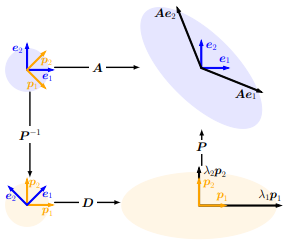
\includegraphics[width=\linewidth, height=4cm, keepaspectratio]{Pictures/maths/Eigendecomposition.png}
            \caption{Eigen Decomposition/ Eigendecomposition}
        \end{figure}
    \end{minipage}
    \hfill
    \begin{minipage}{0.68\linewidth}
        \begin{theorem}[Eigen Decomposition/ Eigendecomposition]
            A square matrix $A \in  R^{n\times n}$ can be factored into
            \[
               \hfill A = PDP^{-1} \hfill
            \]
            where $P \in  R^{n\times n}$ and $D$ is a diagonal matrix whose diagonal entries are the eigenvalues of $A$, if and only if the eigenvectors of $A$ form a basis of $R^n$.
        \end{theorem}
    \end{minipage}    
\end{table}


\begin{enumerate}
    \item \textbf{Top-left to bottom-left}: $P^{-1}$ performs a basis change from the standard basis into the \textbf{eigenbasis}\indexlabel{eigenbasis}

    \item \textbf{Bottom-left to bottom-right}: $D$ performs a scaling along the remapped orthogonal eigenvectors, depicted here by a circle being stretched to an ellipse

    \item \textbf{Bottom-right to top-right}: $P$ undoes the basis change (depicted as a reverse rotation) and restores the original coordinate frame
    
\end{enumerate}

\noindent\textbf{Note}:
\begin{enumerate}
    \item Transformations are applied in \textbf{reverse order}

    \item Let $A$ be the transformation matrix of a linear mapping with respect to the standard basis $e_i$ (blue arrows). 

    \item $P^{-1}$ performs a basis change from the standard basis into the \textbf{eigenbasis}. 

    \item the diagonal $D$ scales the vectors along these axes by the eigenvalues $\lambda_i$. 

    \item $P$ transforms these scaled vectors back into the standard/ canonical coordinates yielding $\lambda_ip_i$
\end{enumerate}

\noindent\textbf{Properties}:
\begin{enumerate}
    \item Diagonal matrices $D$ can efficiently be raised to a power. Therefore, we can find a matrix power for a matrix $A \in R^{n\times n}$ via the eigenvalue decomposition (if it exists) so that 
    \[
        A^k = (PDP^{-1})^k = (PDP^{-1})\overset{k \text{ times}}{\cdots\cdots}(PDP^{-1}) = PD^kP^{-1}
    \]
    Computing $D^k$ is efficient because we apply this operation individually to any diagonal element

    \item Assume that the eigendecomposition $A = PDP^{-1}$ exists. Then:
    \[
    det(A) = det(PDP^{-1}) = det(P)det(D)det(P^{-1}) = det(D) =  
    \hfill (det(P-1) = 1 / det(P))
    \]
    allows for an efficient computation of the determinant of $A$

    \item eigenvalue decomposition requires \textbf{square matrices}

    \item if $A$ is SPD, the decomposition is called "\textbf{spectral decomposition}"\indexlabel{spectral decomposition}

    \item if $\lambda _i$ are eigenvalues of $A$, then $\lambda _i^n$ is eigenvalues of $A^n$
\end{enumerate}


\subsection{Singular Value Decomposition (SVD) ( $A = U\Sigma V^{-1} = U\Sigma V^\top$ )}

\begin{table}[h]
    \begin{minipage}[b]{0.49\linewidth}
        \begin{figure}[H]
            \centering
            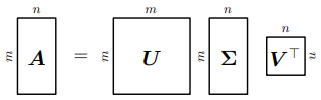
\includegraphics[width=\linewidth, height=4cm, keepaspectratio]{Pictures/maths/svd-1.png}
            \caption{SVD: Matrix Form}
        \end{figure}
    \end{minipage}
    \hfill
    \begin{minipage}[b]{0.49\linewidth}
        \begin{figure}[H]
            \centering
            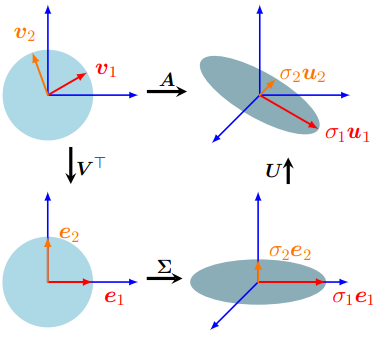
\includegraphics[width=\linewidth, height=4cm, keepaspectratio]{Pictures/maths/svd-2.png}
            \caption{SVD: Transformations}
        \end{figure}
    \end{minipage}
\end{table}

\begin{theorem}[SVD Theorem]
    Let $A \in R^{m\times n}$ be a rectangular matrix of rank $r \in [0, \min(m, n)]$. The SVD of $A$ is a decomposition of the form: $A = U\Sigma V^\top$
\end{theorem}

\begin{enumerate}
    \item \textbf{Top-left to bottom-left}: $V^\top$ performs a basis change in $R^2$ 

    \item \textbf{Bottom-left to bottom-right}: $\Sigma$ scales and maps from $R^2$ to $R^3$. The ellipse in the bottom-right lives in $R^3$. The third dimension is orthogonal to the surface of the elliptical disk.

    \item \textbf{Bottom-right to top-right}: $U$ performs a basis change within $R^3$.
\end{enumerate}

\noindent\textbf{Note}: Transformations are applied in \textbf{reverse order}

\subsubsection{Geometric Interpretation}
$\Phi : R^n \to R^m$\\

\textbf{standard bases}:\\
$B, \tilde{B} \in R^n$\\
$C, \tilde{C} \in R^m$

\vspace{0.2cm}
\noindent The SVD of a matrix can be interpreted as a decomposition of a corresponding linear mapping $\Phi  : R^n \to R^m$ into 3 operations: 
\begin{enumerate}
    \item the SVD performs a basis change via $V^\top $ 

    \begin{enumerate}
        \item scaling and augmentation (or reduction) in dimensionality via the singular value matrix $\Sigma $
    
        \item it performs a second basis change via $U$
    
        \item $V^\top  = V^{-1}$ performs a basis change from $B$ to $\tilde{B}$
    \end{enumerate}

    \item $\Sigma$  scales the new coordinates by the singular values $\Sigma _i$ (and adds or deletes dimensions), i.e., $\Sigma$  is the transformation matrix of $\Phi$  with respect to $\tilde{B}$ and $\tilde{C}$

    \item $U$ performs a basis change in the codomain $R^m$ from $\tilde{C}$ into the canonical basis of $R^m$
\end{enumerate}


\vspace{0.2cm}
\noindent\textbf{Matrix Wise analysis}

\begin{enumerate}
    \item $U \in  R^{m\times m}$ with column vectors $u_i, i = 1, \cdots  , m$
    \begin{enumerate}
        \item orthogonal matrix (SEE: \fullref{Orthogonal Matrix})

        \item $u_i$ are called the \textbf{left-singular vectors}\indexlabel{left-singular vectors}

        \item orthonormal basis $U = (u_1, \cdots  ,u_m)$ of the codomain $R^m$
    \end{enumerate}

    \vspace{0.2cm}
    \item $V \in  R^{n\times n}$ with column vectors $v_j, j = 1, \cdots  , n$
    \begin{enumerate}
        \item orthogonal matrix (SEE: \fullref{Orthogonal Matrix})

        \item $v_j$ are called the \textbf{right-singular vectors}\indexlabel{right-singular vectors}

        \item orthonormal basis $V = (v_1, \cdots  , v_n)$ of the domain $R^n$
    \end{enumerate}

    \vspace{0.2cm}
    \item $\Sigma  \in  R^{m\times n}$ with $\Sigma _{ii} = \sigma _i \geq  0$ and $\Sigma _{ij} = 0, i \neq j$
    \begin{enumerate}
        \item diagonal entries $\sigma _i, i = 1, \cdots  , r$, of $\Sigma$  are called the \textbf{singular values}\indexlabel{singular values}

        \item By convention, the singular values are ordered, i.e., $\sigma _1 \geq  \sigma _2 \geq  \sigma _r \geq  0$.

        \item it is \textbf{unique}

        \item $\Sigma$  has a \textbf{diagonal submatrix} that contains the singular values and needs additional zero padding
        \begin{enumerate}
            \item if $m > n$, then the matrix $\Sigma$  has diagonal structure up to row n and then consists of $0^\top$ row vectors from $n + 1$ to $m$ below so that:
            \[
                \Sigma =
                \begin{bmatrix}
                    \sigma_1 & 0 & 0\\
                    0 & \ddots & 0\\
                    0 & 0 & \sigma_n\\
                    0 & 0 & 0\\
                    0 & \ddots & 0\\
                    0 & 0 & 0\\
                \end{bmatrix}
            \]
    
            \item If $m < n$, the matrix $\Sigma$  has a diagonal structure up to column m and columns that consist of $0$ from $m + 1$ to $n$:
            \[
                \Sigma =
                \begin{bmatrix}
                    \sigma_1 & 0 & 0 & 0 & 0 & 0 \\
                    0 & \ddots & 0 & 0 & \ddots & 0\\
                    0 & 0 & \sigma_n & 0 & 0 & 0\\
                \end{bmatrix}
            \]
        \end{enumerate}
    \end{enumerate}
   
\end{enumerate}


\subsubsection{Constructing SVD}
\begin{enumerate}
    \item If $A$ is SPD:
    \begin{enumerate}
        \item Perform \textbf{Spectral decomposition} (SEE: \fullref{Eigen Decomposition/ Eigendecomposition})
        \[
            A = A^\top = PDP^{-1} = PDP^\top
        \]


        \item $A = U\Sigma V^\top$

        \item $\hfill U = P = V \hfill D = \Sigma \hfill$
    \end{enumerate}

    \item General $A \in R^{m\times n}$:
    \begin{enumerate}
        \item \textbf{Getting right-singular matrix (V):}
        \begin{enumerate}
            \item construct a SPD matrix $A^\top A \in R^{n\times n}$
            \[
                A^\top A = PDP^\top = P \begin{bmatrix}
                    \lambda_1 & \cdots & 0 \\
                    \vdots & \ddots & \vdots \\
                    0 & \cdots & \lambda_n\\
                \end{bmatrix} P^\top
            \]

            \item $P$ : orthogonal matrix, which is composed of the orthonormal eigenbasis

            \item $\lambda_i \geq 0$ : eigenvalues of $A^\top A$

            \item \begin{align*}
                A^\top A 
                &= (U\Sigma V^\top )^\top (U\Sigma V^\top ) \\
                &= V\Sigma ^\top U^\top U\Sigma V^\top \\
                &= V\Sigma ^\top \Sigma V^\top  &&& (U^\top U = I)\\
                &= V \begin{bmatrix}
                    \sigma_1^2 & \cdots & 0 \\
                    \vdots & \ddots & \vdots \\
                    0 & \cdots & \sigma_n^2\\
                \end{bmatrix} V^\top
            \end{align*}

            \item $V^\top = P^\top \Rightarrow V = P$

            \item $\sigma _i^2 = \lambda_i$\\
            eigenvalues of $A^\top A$ are the squared singular values of $\sigma$ 

        \end{enumerate}

        \vspace{0.2cm}
        \item \textbf{Getting left-singular matrix (U):}
        \begin{enumerate}[itemsep=0.2cm]
            \item construct a SPD matrix $AA^\top \in R^{m\times m}$
            
            \item \begin{align*}
                AA^\top 
                &= (U\Sigma V^\top )(U\Sigma V^\top )^\top \\
                &= U\Sigma V^\top V\Sigma^\top U^\top  \\
                &= U\Sigma \Sigma^\top U^\top  &&& (V^\top V = I) \\
                &= U \begin{bmatrix}
                    \sigma_1^2 & \cdots & 0 \\
                    \vdots & \ddots & \vdots \\
                    0 & \cdots & \sigma_m^2\\
                \end{bmatrix} U^\top
            \end{align*}

            \item $U^\top = P^\top \Rightarrow  U = P$
     
            \item $\sigma_j^2 = \lambda_j$
     
            \item eigenvalues of $AA^\top$ are the squared singular values of $\Sigma$

            \item \( \displaystyle u_i = \dfrac{Av_i}{\dnorm{Av_i}} = \dfrac{Av_i}{\sqrt{\lambda_i}} = \dfrac{Av_i}{\sigma_i} \)

            \item \textbf{singular value equation}\indexlabel{singular value equation}: $ Av_i = \sigma_iu_i  \hfill (i = 1, \cdots , r)$
        \end{enumerate}

        \vspace{0.5cm}
        \item \textbf{Getting singular value matrix ($\Sigma$):}
        \begin{enumerate}
            \item $A^\top A$ and $AA^\top$ have \textbf{same} eigenvalues

            \vspace{0.5cm}
            \textbf{Proof}:
            \item $AA^\top x = \lambda x \Rightarrow A^\top A(A^\top x) = A^\top \lambda x = \lambda (A^\top x)$

            \item inner product between $Av_i$ and $Av_j$ must be $0$ for $i \neq j$
            \[
                (Av_i)^\top(Av_j) = v_i^\top (A^\top A)v_j = v_i^\top(\lambda_jv_j) = \lambda_jv_i^\top v_j = 0
            \]

            \item For the case $m \geq r$, it holds that $\dCurlyBrac{Av_1, \cdots , Av_r}$ is a basis of an $r$-dimensional subspace of $R^m$

            \item For $n < m$, Singular value equation holds only for $i \leq  n$, but Singular value equation says nothing about the $u_i$ for $i > n$

            \item for $m < n$, Singular value equation holds only for $i \leq  m$. For $i > m$, we have $Av_i = 0$ and we still know that the $v_i$ form an orthonormal set

            \item (\textbf{Full SVD})\indexlabel{Full SVD} For convenience in notation and abstraction, we use an SVD notation where the SVD is described as having two square left- and right-singular vector matrices, but a non-square singular value matrix. This definition for the SVD is sometimes called the \textbf{full SVD}.

            \item (\textbf{Reduced SVD})\indexlabel{Reduced SVD} SVD can be defined a bit differently and focus on square singular matrices. Then, for $A \in R^{m\times n}$ and $m \geq n$
            \[
                \hfill
                A = U\Sigma V^\top
                \hfill
                A \in  R^{m\times n}
                \hfill
                U \in  R^{m\times n}
                \hfill
                \Sigma  \in  R^{n\times n}
                \hfill
                V \in  R^{n\times n}
                \hfill
            \]

            \item (\textbf{Truncated SVD})\indexlabel{Truncated SVD} TODO

            \item It is possible to define the SVD of a rank-$r$ matrix $A$ so that $U$ is an $m\times r$ matrix, $\Sigma$  a diagonal matrix $r\times r$, and $V$ an $r\times n$ matrix. This construction is very similar to our definition, and ensures that the diagonal matrix $\Sigma$  has only nonzero entries along the diagonal. The main convenience of this alternative notation is that $\Sigma$  is diagonal, as in the eigenvalue decomposition.

            \item Restriction that the SVD for $A$ only applies to $m \times  n$ matrices with m > n is practically unnecessary. When $m < n$, the SVD decomposition will yield $\Sigma$  with more zero columns than rows and, consequently, the singular values $\sigma _{m+1}, \cdots ,\sigma _{n}$ are $0$

            
        \end{enumerate}

        
    \end{enumerate}


\end{enumerate}

\subsubsection{Properties}
\begin{enumerate}
    \item The SVD exists for any matrix $A \in R^{m\times n}$

    \item SVD expresses a change of basis in both the domain and codomain

    \item SVD also supplies an orthonormal basis of the kernel (null space) of $A$, the set of vectors $x$ with $Ax = 0$

    \item Of all possible projections, the SVD minimizes the rank-$k$ approximation error (with respect to the spectral norm) between $A$ and any rank-$k$ approximation \indexlabel{matrix: rank-k approximation}
\end{enumerate}



\subsubsection{SVD Example}
\[
    A = \begin{bmatrix}
        1 & 0 & 1 \\
        -2 & 1 & 0 \\
    \end{bmatrix}
\]

\begin{enumerate}
    \item \textbf{Right-singular vectors as the eigenbasis of $A^\top A$}
    \[
        A^\top A = 
        \begin{bmatrix}
            1 & -2 \\
            0 & 1 \\
            1 & 0 \\
        \end{bmatrix} 
        \begin{bmatrix}
            1 & 0 & 1 \\
            -2 & 1 & 0 \\
        \end{bmatrix}
        =
        \begin{bmatrix}
            5 & -2 & 1 \\
            -2 & 1 & 0 \\
            1 & 0 & 1 \\
        \end{bmatrix}
    \]


    \[
        \renewcommand{\arraystretch}{2}
        A A^\top = 
        \begin{bmatrix}
            5 & -2 & 1 \\
            -2 & 1 & 0 \\
            1 & 0 & 1 \\
        \end{bmatrix}
        =
        \begin{bmatrix}
            \dfrac{5}{\sqrt{30}} & 0 & -\dfrac{1}{\sqrt{6}} \\
            -\dfrac{2}{\sqrt{30}} & \dfrac{1}{\sqrt{5}} & -\dfrac{2}{\sqrt{6}} \\
            \dfrac{1}{\sqrt{30}} & \dfrac{2}{\sqrt{5}} & \dfrac{1}{\sqrt{6}} \\
        \end{bmatrix}
        \begin{bmatrix}
            6 & 0 & 0\\
            0 & 1 & 0 \\
            0 & 0 & 0 \\
        \end{bmatrix}
        \begin{bmatrix}
            \dfrac{5}{\sqrt{30}} & -\dfrac{2}{\sqrt{30}} & \dfrac{1}{\sqrt{30}} \\
            0 & \dfrac{1}{\sqrt{5}} & \dfrac{2}{\sqrt{5}} \\
            -\dfrac{1}{\sqrt{6}} & -\dfrac{2}{\sqrt{6}} & \dfrac{1}{\sqrt{6}}
        \end{bmatrix}
        = PDP^\top
    \]

    \[
        \renewcommand{\arraystretch}{2}
        V = P =
        \begin{bmatrix}
            \dfrac{5}{\sqrt{30}} & 0 & -\dfrac{1}{\sqrt{6}} \\
            -\dfrac{2}{\sqrt{30}} & \dfrac{1}{\sqrt{5}} & -\dfrac{2}{\sqrt{6}} \\
            \dfrac{1}{\sqrt{30}} & \dfrac{2}{\sqrt{5}} & \dfrac{1}{\sqrt{6}} \\
        \end{bmatrix}
    \]

    \vspace{0.5cm}
    \item \textbf{Singular-value matrix:}\\
    As the singular values $\sigma _i$ are the square roots of the eigenvalues of $A^\top A$ we obtain them straight from $D$. Since $rk(A) = 2$, there are only two nonzero singular values: $\sigma _1 = \sqrt{6}$ and $\sigma _2 = 1$.
    \[
        \Sigma = 
        \begin{bmatrix}
            \sqrt{6} & 0 & 0 \\
            0 & 1 & 0 \\
            0 & 0 & 0 \\
        \end{bmatrix}
    \]

    \vspace{0.5cm}
    \item \textbf{Left-singular vectors as the normalized image of the right-singular vectors}
    \[
        \hfill
        \renewcommand{\arraystretch}{2}
        u_1 = \dfrac{Av_1}{\sigma_1} = \dfrac{1}{\sqrt{6}} 
        \begin{bmatrix}
            1 & 0 & 1 \\
            -2 & 1 & 0 \\
        \end{bmatrix}
        \begin{bmatrix}
            \dfrac{5}{\sqrt{30}} \\
            -\dfrac{2}{\sqrt{30}} \\
            \dfrac{1}{\sqrt{30}} \\
        \end{bmatrix}
        = 
        \begin{bmatrix}
            \dfrac{1}{\sqrt{5}} \\
            -\dfrac{2}{\sqrt{5}}
        \end{bmatrix}
        \hspace{0.5cm}
        \renewcommand{\arraystretch}{2}
        u_2 = \dfrac{Av_2}{\sigma_2} = \dfrac{1}{1} 
        \begin{bmatrix}
            1 & 0 & 1 \\
            -2 & 1 & 0 \\
        \end{bmatrix}
        \begin{bmatrix}
            0 \\
            \dfrac{1}{\sqrt{5}} \\
            \dfrac{2}{\sqrt{5}} \\
        \end{bmatrix}
        = 
        \begin{bmatrix}
            \dfrac{2}{\sqrt{5}} \\
            \dfrac{1}{\sqrt{5}}
        \end{bmatrix}
        \hfill
    \]
    \[
        \renewcommand{\arraystretch}{2}
        U = [u_1, u_2] = 
        \begin{bmatrix}
            \dfrac{1}{\sqrt{5}} & \dfrac{2}{\sqrt{5}} \\
            -\dfrac{2}{\sqrt{5}} & \dfrac{1}{\sqrt{5}} \\
        \end{bmatrix}
        = 
        \dfrac{1}{\sqrt{5}}
        \begin{bmatrix}
            1 & {2} \\
            -{2} & {1} \\
        \end{bmatrix}
    \]
    
\end{enumerate}


\subsection{Eigenvalue Decomposition vs. Singular Value Decomposition (SVD)}

\begin{table}[H]
    \begin{tabular}{l l}
        eigendecomposition & $A = PDP^{-1}$ \\
        SVD & $A = U\Sigma V^\top$
    \end{tabular}
\end{table}

\begin{enumerate}
    \item The SVD always exists for any matrix $R^{m\times n}$. The eigendecomposition is only defined for square matrices $R^{n\times n}$ and only exists if we can find a basis of eigenvectors of $R^n$

    \item The vectors in the eigendecomposition matrix $P$ are not necessarily orthogonal, i.e., the change of basis is not a simple rotation and scaling. On the other hand, the vectors in the matrices $U$ and $V$ in the SVD are orthonormal, so they do represent rotations

    \item Both the eigendecomposition and the SVD are compositions of three linear mappings:

    \begin{enumerate}
        \item Change of basis in the domain
    
        \item Independent scaling of each new basis vector and mapping from domain to codomain
    
        \item Change of basis in the codomain
    \end{enumerate}

    \item A key difference between the eigendecomposition and the SVD is that in the SVD, domain and codomain can be vector spaces of different dimensions

    \item In the SVD, the left- and right-singular vector matrices $U$ and $V$ are generally not inverse of each other (they perform basis changes in different vector spaces). In the eigendecomposition, the basis change matrices $P$ and $P^{-1}$ are inverses of each other.

    \item In the SVD, the entries in the diagonal matrix $\Sigma$ are all real and nonnegative, which is not generally true for the diagonal matrix in the eigendecomposition

    \item The SVD and the eigendecomposition are closely related through their projections:
    \begin{enumerate}
        \item The left-singular vectors of $A$ are eigenvectors of $AA^\top$ 
    
        \item The right-singular vectors of $A$ are eigenvectors of $A^\top A$
    
        \item The nonzero singular values of $A$ are the square roots of the nonzero eigenvalues of both $AA^\top$  and $A^\top A$
    \end{enumerate}

    \item For symmetric matrices $A \in  R^{n\times n}$ , the eigenvalue decomposition and the SVD are one and the same (using spectral theorem)

\end{enumerate}



\subsection{LU decomposition ( $A = LU$ ) \cite{wiki/LU_decomposition}} \label{LU decomposition}

\subsubsection{General}
\[
    \displaystyle 
    \begin{bmatrix}
        a_{11} & a_{12} & a_{13} \\
        a_{21} & a_{22} & a_{23}\\
        a_{31} & a_{32} & a_{33}
    \end{bmatrix}
    =
    \begin{bmatrix}
        l _{11} & 0 & 0\\
        l _{21} & l _{22} & 0\\
        l _{31} & l _{32} & l _{33}
    \end{bmatrix}
    \begin{bmatrix}
        u_{11} & u_{12} & u_{13}\\
        0 & u_{22} & u_{23}\\
        0 & 0 & u_{33}
    \end{bmatrix}
\]

\subsubsection{Doolittle Decomposition}\label{LU: Doolittle Decomposition}

\[
    \displaystyle 
    \begin{bmatrix}
        a_{11} & a_{12} & a_{13} \\
        a_{21} & a_{22} & a_{23}\\
        a_{31} & a_{32} & a_{33}
    \end{bmatrix}
    =
    \begin{bmatrix}
        1 & 0 & 0\\
        l _{21} & 1 & 0\\
        l _{31} & l _{32} & 1
    \end{bmatrix}
    \begin{bmatrix}
        u_{11} & u_{12} & u_{13}\\
        0 & u_{22} & u_{23}\\
        0 & 0 & u_{33}
    \end{bmatrix}
\]

\subsubsection{Crout Decomposition}\label{LU: Crout Decomposition}

\[
    \displaystyle 
    \begin{bmatrix}
        a_{11} & a_{12} & a_{13} \\
        a_{21} & a_{22} & a_{23}\\
        a_{31} & a_{32} & a_{33}
    \end{bmatrix}
    =
    \begin{bmatrix}
        l _{11} & 0 & 0\\
        l _{21} & l _{22} & 0\\
        l _{31} & l _{32} & l _{33}
    \end{bmatrix}
    \begin{bmatrix}
        1 & u_{12} & u_{13}\\
        0 & 1 & u_{23}\\
        0 & 0 & 1
    \end{bmatrix}
\]



\section{Matrix Approximation \cite{mfml-1}}\label{Matrix Approximation}

SVD allows us to represent a matrix $A$ as a sum of simpler (low-rank) matrices $A_i$, which lends itself to a matrix approximation scheme that is cheaper to compute than the \textbf{full SVD}.

\[
    A_i := u_iv_i^\top \hfill \text{(rank-$1$ matrix $A_i \in R^{m\times n}$)}
\]

which is formed by the outer product of the $i$th orthogonal column vector of $U$ and $V$

\[
    \displaystyle
    A = 
    \sum_{i=1}^{r} \sigma_iu_iv^\top
    =
    \sum_{i=1}^{r} \sigma_iA_i
    \hfill
    (rk(A)=r)
\]
where the outer-product matrices $A_i$ are weighted by the $i$th singular value $\sigma_i$\\
All terms $\displaystyle \sum_{i=1}^{r} u_iv^\top$ vanish for $i \neq j$ because $\Sigma$ is a diagonal matrix. Any terms $i > r$ vanish because the corresponding singular values are $0$.

\vspace{0.2cm}
\textbf{rank-k approximation}:
\[
    \displaystyle
    \hat{A}(k) = 
    \sum_{i=1}^{k} \sigma_iu_iv^\top
    =
    \sum_{i=1}^{k} \sigma_iA_i
    \hfill
    (rk(\hat{A}(k))=k)
    (k < r)
\]

\begin{theorem}[Eckart-Young Theorem]\indexlabel{rank-k approximation: Eckart-Young Theorem}
    Consider a matrix $A \in R^{m\times n}$ of rank $r$ and let $B \in R^{m\times n}$ be a matrix of rank $k$. For any $k \leq r$ with $\hat{A}(k) = \sum_{i=1}^{k} \sigma_iu_iv^\top$ it holds that:
    \begin{enumerate}
        \item $\displaystyle \hat{A}(k) = \arg\min_{rk(B)=k} \dnorm{A-B}_2$

        \item $\displaystyle \dnorm{A-\hat{A}(k)}_2 = \sigma_{k+1} \hfill (\text{rank-r approximation error})$\indexlabel{rank-r approximation error}
    \end{enumerate}
\end{theorem}

\begin{enumerate}
    \item We can interpret the rank-$k$ approximation obtained with the SVD as a projection of the full-rank matrix $A$ onto a lower-dimensional space of rank-at-most-$kS$ matrices.

    \item \[
        \displaystyle
        A - \hat{A}(k) = 
        \sum_{i=k+1}^{r} \sigma_iu_iv^\top
    \]

    \item $\sigma_{k+1}$ : spectral norm of the difference matrix

    \item let matrix $B$ with $rk(B) \leq k$, such that $\dnorm{A-B}_2 < \dnorm{A-\hat{A}(k)}_2$ then there exists an at least $(n - k)$-dimensional null space $Z \subseteq R^n$, such that $x \in Z$ implies that $Bx = 0$. Then it follows that $\dnorm{Ax}_2=\dnorm{(A-B)x}_2$ and by using a version of the Cauchy-Schwarz inequality  that encompasses norms of matrices, we obtain $\dnorm{Ax}_2 \leq \dnorm{A-B}_2\dnorm{x}_2 \leq \sigma_{k+1}\dnorm{x}_2$

    \item there exists a $(k + 1)$-dimensional subspace where $\dnorm{Ax}_2 \geq \sigma _{k+1}\dnorm{x}_2$, which is spanned by the right-singular vectors $v_j, j \leq k + 1$ of $A$

    \item Adding up dimensions of these two spaces yields a number greater than $n$, as there must be a non-zero vector in both spaces. This is a \textbf{contradiction} of the \textbf{rank-nullity theorem}

    \item We can use SVD to reduce a rank-$r$ matrix $A$ to a rank-k matrix  in a principled, optimal (in the spectral norm sense) manner. We can interpret the approximation of $A$ by a rank-$k$ matrix as a form of \textbf{lossy compression}\indexlabel{rank-k approx: lossy compression}.

\end{enumerate}



\section{Gradients of Matrices}
\subsection{With Respect to Matrix}
if we compute the gradient of an $m \times  n$ matrix $A$ with respect to a $p \times  q$ matrix $B$, the resulting Jacobian would be $(m\times n)\times (p\times q)$, i.e., a four-dimensional tensor $J$, whose entries are given as $J_{ijkl} = \partial A_{ij}/\partial B_{kl}$



























    \chapter{Vector \cite{mfml-1}}\label{chapter: Vector}

\section*{Intro \cite{mfml-1}}
\begin{table}[H]
    \begin{tabular}{l l}
        rows/ row vectors & $(1, n)$-matrices are called rows \\

        columns/ column vectors & $(m, 1)$-matrices are called columns \\
    \end{tabular}
\end{table}

Alternate Definition: SEE \fullref{vectors}


\section{Outer Product ( $a\otimes b= \mathbf{ab^\top} \in \mathbb{R}^{m\times n}$ ) \cite{mfml-1}} \label{vector: Outer Product}
\[
    a\otimes b= \mathbf{ab^\top} = 
    \begin{bmatrix}
        a_1\\
        \vdots\\
        a_m
    \end{bmatrix}
    \begin{bmatrix}
        b_n & \cdots & b_n
    \end{bmatrix}
    =
    \begin{bmatrix}
        a_1 b_1 & a_1 b_2 & \cdots & a_1 b_n\\
        a_2 b_1 & a_2 b_2 & \cdots & a_2 b_n\\
        \vdots & \vdots & \ddots & \vdots \\
        a_m b_1 & a_m b_2 & \cdots & a_m b_n\\
    \end{bmatrix} \in \mathbb{R}^{m\times n}
\]
\[
    (a\otimes b)_{ij} = a_i b_j
\]

\section{Inner/ Scalar /Dot Product ( $\langle a, b \rangle =a\cdot b = \mathbf{a^\top b} \in \mathbb{R}$ ) \cite{mfml^{-1}wiki/Dot_product}} \label{vector: Inner/ Scalar /Dot Product}

The dot product or scalar product is an algebraic operation that takes two vectors of equal length, and returns a \textbf{single number}.
the dot product between two vectors $a, b$ is denoted by $a^\top b$ or $\langle a, b\rangle \in R$:
\[
    \displaystyle
    \langle a, b \rangle =
    a\cdot b = 
    \mathbf{a^\top b} =
    \sum_{i=1}^{n} a_i b_i
    \in \mathbb{R}
\]


\section{Codirection}\label{Codirection}
Two vectors that point in the \textbf{same direction} are called codirected. 


\section{Collinearity}\label{Collinearity}
Two vectors are collinear if they point in the \textbf{same or the opposite direction}.


\section{Partial Differentiation ( $\partial f/\partial x$ )} \label{vectors: Partial Differentiation}

For a function $f : R^n \to R$, $x \mapsto f(x)$, $x \in R^n$ of $n$ variables $x_1, \cdots , x_n$ we define the partial derivatives as
\[
    f = f(x) = f(x_1, \cdots , x_n)
\]
\[
    \displaystyle
    \begin{matrix}
    \dfrac{\partial f}{\partial x_1} = 
    \lim_{h\to 0} \dfrac{f(x_1+h, \cdots , x_n) - f(x)}{h} \\
    \vdots\\
    \dfrac{\partial f}{\partial x_n} = 
    \lim_{h\to 0} \dfrac{f(x_1, \cdots , x_n+h) - f(x)}{h} \\
    \end{matrix}
\]

where $n$ is the number of variables and $1$ is the dimension of the \textbf{image/ range/ codomain} of $f$ \indexlabel{function of vector: image/ range/ codomain}.


\subsection{Rules of Partial Differentiation}

\begin{table}[h]
    \centering
    \begin{tabular}{|p{2.5cm}|p{12.5cm}|}
        \hline
        Sum Rule & \begin{minipage}{12cm}
            \vspace{-0.1cm}
            \[
                \dfrac{\partial}{\partial x}(f(x) + g(x))
                = 
                \dfrac{\partial f(x)}{\partial x} +
                \dfrac{\partial g(x)}{\partial x}
            \]
            \vspace{0.1cm}
        \end{minipage} \\
        \hline
        Product Rule & \begin{minipage}{12cm}
            \vspace{-0.1cm}
            \[
                \dfrac{\partial}{\partial x}(f(x)g(x))
                = 
                \dfrac{\partial f(x)}{\partial x}g(x) +
                f(x)\dfrac{\partial g(x)}{\partial x}
            \]
            \vspace{0.1cm}
        \end{minipage} \\
        \hline
        Chain Rule & \begin{minipage}{12cm}
            \vspace{-0.1cm}
            \[
                \dfrac{\partial}{\partial x}((g \circ f)(x))
                = 
                \dfrac{\partial}{\partial x}(g(f(x))
                =
                \dfrac{\partial g(x)}{\partial f(x)}
                \dfrac{\partial f(x)}{\partial x}
            \]
            
            Consider a function $f(x_1, x_2) = f : R^2 \to R$ of two variables $x_1, x_2$. Furthermore, $x_1(t)$ and $x_2(t)$ are themselves functions of $t$. To compute the gradient of $f$ with respect to $t$:
            \[
                \dfrac{df}{dt}
                = \begin{bmatrix}
                    \dfrac{\partial f}{\partial x_1} &
                    \dfrac{\partial f}{\partial x_2}
                \end{bmatrix}
                \begin{bmatrix}
                    \dfrac{\partial x_1(t)}{\partial t}\\
                    \dfrac{\partial x_2(t)}{\partial t}
                \end{bmatrix}
                = \dfrac{\partial f}{\partial x_1}
                \dfrac{\partial x_1}{\partial t}
                +
                \dfrac{\partial f}{\partial x_2}
                \dfrac{\partial x_2}{\partial t}
            \]

            If $f(x_1, x_2)$ is a function of $x_1$ and $x_2$, where $x_1(s, t)$ and $x_2(s, t)$ are themselves functions of two variables $s$ and $t$, the chain rule yields the partial derivative:
            \[
                \dfrac{df}{ds}
                = \dfrac{\partial f}{\partial x_1}
                \dfrac{\partial x_1}{\partial s}
                +
                \dfrac{\partial f}{\partial x_2}
                \dfrac{\partial x_2}{\partial s}
            \]
            \[
                \dfrac{df}{dt}
                = \dfrac{\partial f}{\partial x_1}
                \dfrac{\partial x_1}{\partial t}
                +
                \dfrac{\partial f}{\partial x_2}
                \dfrac{\partial x_2}{\partial t}
            \]
            \vspace{0.1cm}
        \end{minipage} \\
        \hline
    \end{tabular}
\end{table}


\section{Gradient of vector function ( $\nabla _xf = \operatorname{grad} f$ )}\label{Gradient of vector function}

For a function $f : R^n \to R^n$, $x \to f(x)$, $x \in R^n$ of $n$ variables $x_1, \cdots , x_n$ we define the gradient as

\[
    \nabla_x f = 
    \operatorname{grad} f = 
    \dfrac{df}{dx} =
    \begin{bmatrix}
        \dfrac{\partial f(x)}{\partial x_1} &
        \dfrac{\partial f(x)}{\partial x_2} &
        \cdots &
        \dfrac{\partial f(x)}{\partial x_n}
    \end{bmatrix}
    \in R^{1\times n}
\]

\noindent where,
\begin{enumerate}
    \item $n$ is the number of variables and $1$ is the dimension of the \textbf{image/ range/ codomain} of f \indexlabel{gradient of vector fn: image/ range/ codomain}. 

    \item It is collection of partial derivatives  

    \item The row vector is called the gradient of $f$ or the \textbf{Jacobian} and is the generalization of the derivative.

    \item This definition of the Jacobian is a special case of the general definition of the Jacobian for vector-valued functions as the collection of partial
\end{enumerate}

If $f(x_1, x_2)$ is a function of $x_1$ and $x_2$, where $x_1(s, t)$ and $x_2(s, t)$ are themselves functions of two variables $s$ and $t$, the chain rule yields the gradient:
\[
    \renewcommand{\arraystretch}{2}
    \dfrac{df}{d(s,t)} =
    \dfrac{\partial f}{\partial x}
    \dfrac{\partial x}{\partial (s,t)} =
    \begin{bmatrix}
        \dfrac{\partial f}{\textcolor{blue}{\partial x_1}} &
        \dfrac{\partial f}{\textcolor{Maroon}{\partial x_2}}
    \end{bmatrix}
    \begin{bmatrix}
        \textcolor{blue}{\dfrac{\partial x_1}{\partial s}} &
        \textcolor{blue}{\dfrac{\partial x_1}{\partial t}}\\
        \textcolor{Maroon}{\dfrac{\partial x_2}{\partial s}} &
        \textcolor{Maroon}{\dfrac{\partial x_2}{\partial t}}\\
    \end{bmatrix}
\]

\section{Vector-Valued Functions}\label{Vector-Valued Functions}
For a function $f : Rn -> Rm$ and a vector $x = [x_1, \cdots , x_n]^\top \in R^n$, the corresponding vector of function values is given as:
\[
    f(x) = 
    \begin{bmatrix}
        f_1(x)\\
        \vdots\\
        f_m(x)\\
    \end{bmatrix}
    \in R^m
\]

where:
\begin{enumerate}
    \item $f =  [f_1, \cdots , f_m]^\top$

    \item $f_i$ or $f_i(x) : R^n \to R$ that maps $x$ onto $R$
\end{enumerate}

\section{Partial Derivative of Vector-Valued Functions ( $\partial f(x)/\partial x_i$ )}\label{Partial Derivative of Vector-Valued Functions}

\[
    \dfrac{\partial f}{\partial x_i}=
    \begin{bmatrix}
        \dfrac{\partial f_1}{\partial x_i} \\
        \vdots \\
        \dfrac{\partial f_m}{\partial x_i}
    \end{bmatrix} =
    \begin{bmatrix}
        \displaystyle\lim_{h \to 0} \dfrac{ f_1(x_1,\cdots ,x_{i-1},x_i+h,x_{i+1},\cdots x_n) - f_1(x)}{h} \\
        \vdots \\
        \displaystyle\lim_{h \to 0} \dfrac{f_m(x_1,\cdots ,x_{i-1},x_i+h,x_{i+1},\cdots x_n) - f_m(x)}{h}
    \end{bmatrix}
    \in R^m
\]


\section{Jacobian/ Gradient of Vector-Valued Functions ( $J = \nabla_x f = df(x)/dx$ )}\label{Jacobian/ Gradient of Vector-Valued Functions}

The collection of all \textbf{first-order partial derivatives} of a vector-valued function $f : R^n \to R^m$ is called the Jacobian. The Jacobian $J$ is an $m \times n$ matrix, which we define and arrange as follows:

\[
    J = \nabla_x f =
    \dfrac{df(x)}{dx} =
    \begin{bmatrix}
        \textcolor{blue}{\dfrac{\partial f(x)}{\partial x_1}} &
        \cdots &
        \textcolor{Maroon}{\dfrac{\partial f(x)}{\partial x_n}}
    \end{bmatrix} =
    \begin{bmatrix}
        \textcolor{blue}{\dfrac{\partial f_1(x)}{\partial x_1}} &
        \cdots &
        \textcolor{Maroon}{\dfrac{\partial f_1(x)}{\partial x_n}}\\
        \vdots & \ddots & \vdots \\
        \textcolor{blue}{\dfrac{\partial f_m(x)}{\partial x_1}} &
        \cdots &
        \textcolor{Maroon}{\dfrac{\partial f_m(x)}{\partial x_n}}\\
    \end{bmatrix}
    \in R^{m\times n}
\]

\begin{enumerate}
    \item we use the numerator layout of the derivative, i.e., the derivative $df/dx$ of $f \in R^m$ with respect to $x \in R^n$ is an $m \times n$ matrix, where the elements of $f$ define the rows and the elements of $x$ define the columns of the corresponding Jacobian

    \item there also exists also the denominator layout, which is the transpose of the numerator layout

    \item default = numerator layout

    \item Jacobian determinant $\dabs{det(J)}$ is the factor by which areas or volumes are scaled when coordinates are transformed.
\end{enumerate}


\section{Higher-Order Derivatives}\label{Higher-Order Derivatives}

\begin{table}[H]
    \centering
    \renewcommand{\arraystretch}{2.5}
    \begin{tabular}{|p{3cm}|p{12cm}|}
        \hline
        $\dfrac{\partial^2 f}{\partial x^2}$ & second partial derivative of $f$ with respect to $x$ \\
        \hline
        $\dfrac{\partial^n f}{\partial x^n}$ & $n$th partial derivative of $f$ with respect to $x$ \\
        \hline
        $\dfrac{\partial^2 f}{\partial y \partial x} = \dfrac{\partial}{\partial y}\dParenBrac{ \dfrac{\partial f}{\partial x} }$ & partial derivative obtained by first partial differentiating with respect to $x$ and then with respect to $y$ \\
        \hline
        $\dfrac{\partial^2 f}{\partial x \partial y} = \dfrac{\partial}{\partial x}\dParenBrac{ \dfrac{\partial f}{\partial y} }$ & partial derivative obtained by first partial differentiating by $y$ and then $x$ \\
        \hline
    \end{tabular}
    \caption{Higher-Order Derivatives}
\end{table}

\begin{enumerate}
    \item If $f(x, y)$ is a twice (continuously) differentiable function, then 
    $\dfrac{\partial^2 f}{\partial x \partial y} = \dfrac{\partial^2 f}{\partial y \partial x}$

\end{enumerate}


\section{Hessian/ Hessian Matrix ( $H = \nabla_{x,y}^2f$ )}\label{Hessian/ Hessian Matrix}
The Hessian is the collection of all \textbf{second-order partial derivative}.
\[
    H = 
    \begin{bmatrix}
        \dfrac{\partial^2 f}{\partial x^2} &
        \dfrac{\partial^2 f}{\partial x \partial y}\\
        \dfrac{\partial^2 f}{\partial y \partial x} &
        \dfrac{\partial^2 f}{\partial y^2}
    \end{bmatrix}
\]


\begin{enumerate}
    \item H is symmetric

    \item for $x \in R^n$ and $f : R^n \to R$, the Hessian is an $n \times n$ matrix

    \item The Hessian measures the curvature of the function locally around $(x, y)$.

    \item (\textbf{Hessian of a Vector Field}\indexlabel{Hessian of a Vector Field}). If $f : R^n \to R^m$ is a \textbf{vector field}\indexlabel{vector field}, the Hessian is an $(m \times n \times n)$-tensor
\end{enumerate}



\section{Gradient/ Derivative Common Formulas}\label{matrix-vector: Gradient/ Derivative Common Formulas}

\begin{enumerate}[itemsep=0.2cm]
    \subsection{Matrix-vector}
    
    \item \( d(Ax)/dx = A \)

    \item $d(Ax)/dA = v^\top\otimes I $
    
    \item \( \partial (A^{-1})/\partial y = A^{-1}\)

    \subsection{matrix-matrix}
    \item \(
        d(XX)/dX = A^\top \otimes I+I\otimes A
    \)
    
    \item  $d(X^\top X)/dX = ??$
    
    \item  $d(XX^\top )/dX = ??$

    \subsection{vector-vector}
    \item  $\partial (a^\top x)/\partial x = a^\top$

    \item $\partial (x^\top a)/\partial x = a^\top$

    \item  $d(x^\top x)/dx = 2x$

    \item  $d(xx^\top)/dx = ??$

    \item  \(
        \partial (x^\top Bx)/\partial x = \begin{cases}
            x^\top(B + B^\top) & \text{ general}\\
            2x^\top B & \text{ $B$ is symmetric}
        \end{cases}
    \)

    \item  $\partial (a^\top X^{-1}b)/\partial X = -(X^{-1})^\top ab^\top (X^{-1})^\top$

    \item  $d(x^\top Ax)/dA = xx^\top $

    \item  $\partial (a^\top Xb)/\partial X = ab^\top$

    \item  $\partial [(x - As)^\top W(x - As)]/\partial s = -2(x - As)^\top WA$ $\hfill$ ($W$ is symmetric)

    \item $\partial (f(X)^\top)/\partial X = (\partial f(X)/\partial X)^\top$

    \item $\partial (f(X)^{-1})/\partial X = -f(X)^{-1}\cdot  (\partial f(X)/\partial X) \cdot  f(X)^{-1}$

    \item $\partial [tr(f(X))]/\partial X = tr(\partial f(X)/\partial X)$

    \item $\partial [det(f(X))]/\partial X = det(f(X)) \cdot  tr(f(X)^{-1}\cdot  (\partial f(X)/\partial X))$


\end{enumerate}


\section{Automatic Differentiation (AutoDiff) \cite{mfml-1}} \label{Automatic Differentiation}

SEE: \fullref{Automatic Differentiation (AutoDiff) VS Backpropagation VS Chain Rule}

\begin{enumerate}
    \item Automatic differentiation is different from symbolic differentiation and numerical approximations of the gradient, e.g., by using finite differences.

    \item We can think of automatic differentiation as a set of techniques to numerically (in contrast to symbolically) evaluate the exact (up to machine precision) gradient of a function by working with intermediate variables and applying the chain rule. 

    \item Automatic differentiation applies a series of elementary arithmetic operations, e.g., addition and multiplication and elementary functions, e.g., sin, cos, exp, log. 

    \item By applying the chain rule to these operations, the gradient of quite complicated functions can be computed automatically.

    \item \textbf{backpropagation} is a \textbf{special case} of a general technique in numerical analysis called automatic differentiation

    \item \textbf{NOT ALL} computer programs can be automatically differentiated, e.g., if we cannot find differential elementary functions
\end{enumerate}

Let $x_1, \cdots , x_d$ be the input variables to the function, $x_{d+1}, \cdots , x_{D-1}$ be the intermediate variables, and $x_D$ the output variable. Then the computation graph can be expressed as follows:


\subsubsection*{forward propagation}
\[
    x_i = g_i(x_{P_a(x_i)}) \hfill (i = d+1, \cdots, D)
\]
where
\begin{enumerate}
    \item $g_i(\cdot)$ are \textbf{elementary functions}

    \item $x_{P_a(xi)}$ are the \textbf{parent nodes} of the variable $x_i$ in the \textbf{graph}

\end{enumerate}

\subsubsection*{backpropagation}
\[
    f = x_D \Rightarrow \dfrac{\partial f}{\partial x_D} = 1
\]
\[
    \displaystyle 
    \dfrac{\partial f}{ \partial x_i} = 
    \sum_{x_j:x_i\in P_a(x_j)} \dfrac{\partial f}{\partial x_j} \dfrac{\partial x_j}{\partial x_i} =
    \sum_{x_j:x_i\in P_a(x_j)} \dfrac{\partial f}{\partial x_j} \dfrac{\partial g_j}{\partial x_i} 
\]

  

\subsubsection*{Example}

\[
    \hfill
    f(x) = \sqrt{x^2 + exp(x^2)} + cos(x^2 + exp(x^2))
    \hfill
\]
\begin{table}[H]
    \begin{minipage}{0.59\linewidth}
        \begin{figure}[H]
            \centering
            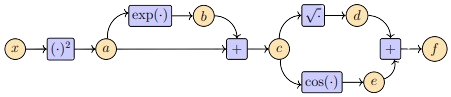
\includegraphics[width=\linewidth, height=2cm, keepaspectratio]{Pictures/maths/AutoDiff-ex5.14.png}
        \end{figure}
    \end{minipage}
    \hfill
    \begin{minipage}{0.39\linewidth}
        \begin{alternateColorTable}
        \begin{table}[H]
            \centering
            \renewcommand{\arraystretch}{2}
            \begin{tabular}{p{2.5cm} l}
                \tableHeaderRow
                \textbf{Forward propagation} & \textbf{Backward Propagation} \\ \hline
                
                $a = x^2$ & $\dfrac{\partial a}{\partial x} = 2x$ \\
        
                $b = exp(a) = e^a$ & $\dfrac{\partial b}{\partial a} = b = e^a$\\
        
                $c = a+b$ & $
                \dfrac{\partial c}{\partial a}=1 
                \hspace{0.5cm} 
                \dfrac{\partial c}{\partial b}=1$ \\
        
                $d = \sqrt{c} = c^{0.5}$ & $\dfrac{\partial d}{\partial c}=0.5c^{-0.5} = \dfrac{1}{2\sqrt{c}}$ \\
        
                $e = cos(c)$ & $\dfrac{\partial e}{\partial c} = -sin(c)$\\
        
                $f = d + e$ & $
                \dfrac{\partial f}{\partial d} = 1 
                \hspace{0.5cm} 
                \dfrac{\partial f}{\partial e} = 1$
            \end{tabular}
        \end{table}
        \end{alternateColorTable}
    \end{minipage}
\end{table}

\begin{alternateColorTable}
\begin{table}[H]
    \renewcommand{\arraystretch}{2}
    \centering
    \begin{tabular}{l l l}
        \tableHeaderRow
        & \textbf{Calculation} & \textbf{Evaluation} \\
        \hline
    
        $\dfrac{\partial f}{\partial c}$ & 
        $=
            \dfrac{\partial f}{\partial d}
            \dfrac{\partial d}{\partial c}
            +
            \dfrac{\partial f}{\partial e}
            \dfrac{\partial e}{\partial c}
        $ &
        $=
            1\cdot \dfrac{1}{2\sqrt{c}}+
            1\cdot (-sin(c))
        $\\

        $\dfrac{\partial f}{\partial b}$ &
        $=
            \dfrac{\partial f}{\partial c} 
            \dfrac{\partial c}{\partial b}
        $ &
        $
            = \dfrac{\partial f}{\partial c} \cdot 1
        $\\

        $\dfrac{\partial f}{\partial a}$ &
        $=
            \dfrac{\partial f}{\partial b} 
            \dfrac{\partial b}{\partial a}
            +
            \dfrac{\partial f}{\partial c} 
            \dfrac{\partial c}{\partial a}
        $ &
        $
            = \dfrac{\partial f}{\partial b}\exp(a)+
            \dfrac{\partial f}{\partial c}\cdot 1
        $\\

        $\dfrac{\partial f}{\partial x}$ &
        $=
            \dfrac{\partial f}{\partial a}
            \dfrac{\partial a}{\partial x}
        $ &
        $=\dfrac{\partial f}{\partial a}\cdot 2x$
    \end{tabular}
\end{table}
\end{alternateColorTable}











    \chapter{Statistics: Sampling}\label{Statistics: Sampling}

\begin{figure}[h]
    \centering
    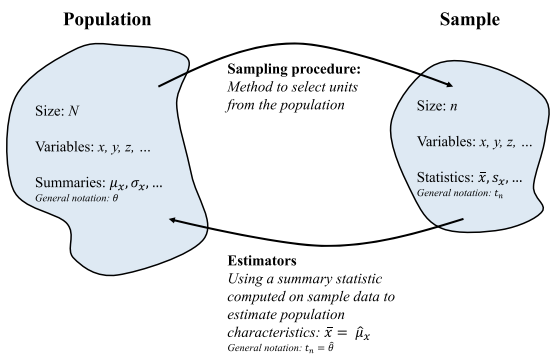
\includegraphics[width=\linewidth, height=4cm, keepaspectratio]{Pictures/statistics/population-and-sample.png}
\end{figure}

\begin{table}[h]
    \centering
    \begin{tabular}{|l|c|c|}
        \hline

        & \textbf{Population} & \textbf{Sample}\\
        \hline

        \textbf{Size} & $N$ & $n$ \\
        \hline

        \textbf{Variables} & $x,y,z,\cdots$ & $x,y,z,\cdots$ \\
        \hline

        \textbf{Summaries/ Statistics} & $\mu_x,\sigma_x,\cdots$ & $\bar{x}, s_x, \cdots$\\
        \hline

        \textbf{General Notation} & $\theta$ & $t_n$\\
        \hline
    \end{tabular}
\end{table}


\section{Convenience Sampling \cite{ism-1}} \label{Convenience Sampling}

\begin{enumerate}
    \item collects only units from the population that can be \textbf{easily obtained}

    \item may provide a \textbf{biased} sample

    \item often justified by using the argument of \textbf{population homogeneity}
\end{enumerate}

\section{Haphazard Sampling \cite{ism-1}}
\label{Haphazard Sampling}

\begin{enumerate}
    \item Despite the feeling of randomness when performing haphazard sampling, often the resulting sample is not truly random.

\end{enumerate}


\section{Purposive Sampling \cite{ism-1}}\label{Purposive Sampling}

\begin{enumerate}
    \item tries to sample units for a specific purpose. 

    \item This means that the collection of units is focused on one or more particular characteristics and hence it implies that only units that are more alike are sampled.
\end{enumerate}


\section{Simple Random Sampling \cite{ism-1}}\label{Simple Random Sampling}

\renewcommand{\arraystretch}{2.5}
\begin{longtable}{|p{5cm}|p{9cm}|}
    \hline\endfirsthead
    \hline\endhead
    \hline\endfoot
    \hline\endlastfoot

    \textbf{Number of possible samples} & \( \dfrac{N!}{n!(N-n)!} \) \\
    \hline

    \textbf{Probability that $S_k$ is selected} & $\pi_k = \dfrac{1}{K}$ \\
    \hline

    \textbf{Probability that a specific unit is part of the sample} & $\dfrac{n}{N}$ \\
    \hline

    \textbf{Mean ($\mathbb{E}(T)$)} & $
        \mathbb{E}(T) = 
        \dfrac{1}{K} \dsum_{k=1}^{K}
        \bar{x}_k 
        =
        \dfrac{1}{nK} \dsum_{k=1}^{K}
        \dsum_{i \in S_k} x_i
        =
        \dfrac{1}{N} \dsum_{i=1}^{N} x_i
        = \mu
    $ \\[2ex]
    \hline

    \textbf{Estimator of Mean ($\bar{x}_k$)} & $
        \bar{x}_k=
        \dfrac{1}{n} \dsum_{i=1}^{n} x_i
    $ \\[2ex]
    \hline

    \textbf{Bias} & $
        bias(c\bar{x}_k) = (c-1)\mu
        \quad\quad\quad
        bias(\bar{x}_k) = 0
    $ \\[1ex]
    \hline

    \textbf{MSE ($MSE(c\bar{x}_k)$)} & $
        MSE(c\bar{x}_k) 
        = [(c-1)\mu]^2 +
        c^2 \sigma^2 \dParenBrac{\dfrac{N}{N-1} \right)\left( 1-\dfrac{n}{N} }\dfrac{1}{n}
    $\\[1ex]
    & $MSE(\bar{x}_k) 
        = \sigma^2 \dParenBrac{\dfrac{N}{N-1} \right)\left( 1-\dfrac{n}{N} }\dfrac{1}{n}$ \\[1ex]
    \hline

    \textbf{Estimator of MSE ($\hat{MSE}(\bar{x}_k)$)} & $
        \hat{MSE}(\bar{x}_k) = \dParenBrac{\dfrac{N-n}{Nn} }s_k^2
    $\\[1ex]
    \hline

    \textbf{Variance ($\sigma^2$)} & $
        \sigma^2 = \dfrac{1}{N} \dsum_{i=1}^{N}
        (x_i - \mu)^2
    $\\[1ex]
    \hline

    \textbf{Estimator of Variance ($s_k^2$)} & $
        s_k^2 = \dParenBrac{\dfrac{1}{n-1}} \dsum_{i\in S_k}
        (x_i - \bar{x}_k)^2
    $\\[1ex]
    \hline

    \textbf{SE ($SE(c\bar{x}_k)$)} & $
        SE(c\bar{x}_k) = \sqrt{
            c^2 \sigma^2 
            \dParenBrac{ \dfrac{N}{N-1} }
            \dParenBrac{ 1-\dfrac{n}{N} }
            \dfrac{1}{n}
        }
    $\\[1ex]
    \hline
\end{longtable}

\section{Systematic Sampling \cite{ism-1}}\label{Systematic Sampling}

\begin{enumerate}
    \item Population should be divided into $n$ groups and the order of the units (if some order exists) should be maintained (or otherwise fix the order).

    \item each group consists of $m$ units (thus the population size is $N = nm$) \textbf{ordered} from $1$ to $m$ in each group.
    \[
        m \in \dCurlyBrac{1,2,\cdots,N}
    \]

    \item from each of the $n$ groups the $k$th unit is collected, forming the sample of $n$ units. 
    \[
        S_k = \dCurlyBrac{ k, k+m,k+2m,\cdots,k+(n-1)m }
        \hfill
        (k \in \dCurlyBrac{1,2,\cdots,m})
    \]
\end{enumerate}

\begin{alternateColorTable}
\begin{longtable}{|p{5cm}|p{9cm}|}
    \hline\endfirsthead
    \hline\endhead
    \hline\endfoot
    \hline\endlastfoot

    \textbf{Probability of selecting $S_k$} & $\dfrac{1}{m}$\\[1ex]
    \hline

    \textbf{Mean ($\mu$)} & $
        \mu = \dfrac{1}{N}
        \dsum_{h=1}^{m}
        \dsum_{i=1}^{n} 
        x_{h+m(i-1)}
    $\\[1ex]
    \hline

    \textbf{Estimator of Mean ($\bar{x}_k$)} & $
        \bar{x}_k = 
        \dfrac{1}{n} \dsum_{i=1}^{n}
        x_{h+m(i-1)}
    $\\[1ex]
    \hline

    \textbf{Variance ($\sigma^2$)} & $
        \sigma^2 = 
        \dfrac{1}{N}
        \dsum_{k=1}^{m}
        \dsum_{i=1}^{n}
        (x_{k+m(i-1)} - \mu)^2
    $\\[1ex]
    \hline

    \textbf{Estimator of Variance ($s_k^2$)} & $
        s_k^2 = \dParenBrac{\dfrac{1}{n-1}}
        \dsum_{i=1}^{n}
        (x_{k+m(i-1)} - \bar{x}_k)^2
    $\\[1ex]
    \hline

    \textbf{Bias} & $bias(\bar{x}_k) = 0$\\
    \hline

    \textbf{MSE} & $
        MSE = \sigma^2 -
        \dfrac{1}{N}
        \dsum_{h=1}^{m}
        \dsum_{i=1}^{n}
        (x_{h+m(i-1)} - \bar{x}_h)^2
    $\\[1ex]
    \hline
\end{longtable}
\end{alternateColorTable}

\section{Stratified Sampling \cite{ism-1}}\label{Stratified Sampling}

\begin{enumerate}
    \item numbers of units across the \textbf{subpopulations} $S_h$ (called \textbf{strata}\indexlabel{strata}) are (substantially) different $N_h$

    \item selecting the same fraction/ proportion of the units from each stratum we are certain that each stratum is included in the sample, and represents the population

    \item If the ratio of the sample size $n_h$ and stratum size $N_h$ is the same across all strata, each unit in the population has the same probability of being collected in the sample. This type of stratified sampling is called \textbf{proportional stratified sampling}\indexlabel{proportional stratified sampling}.

    \item[] $S_h = \dCurlyBrac{ S_{h,1}, S_{h,2},\cdots, S_{h,N_h} }$

    \item[] $K_h = \dfrac{N_h!}{n_h!(N_h-n_h)!}$

    \item[] $w_h = \dfrac{N_h}{N}$

    \item[] $
        K_S = 
        \dfrac{N_1!}{n_1!(N_1-n_1)!} 
        \times
        \dfrac{N_1!}{n_1!(N_1-n_1)!} 
        \times
        \cdots
        \times
        \dfrac{N_M!}{n_M!(N_M-n_M)!}
        =
        \dprod_{M}^{i=1} \dfrac{N_i!}{ni!(N_i-n_i)!}
    $

    \item[] $
        \dsum_{i=1}^{M} N_i = N
        \quad\quad
        \dsum_{i=1}^{M} n_i = n
    $


\end{enumerate}

\begin{alternateColorTable}
\begin{longtable}{|p{5cm}|p{9cm}|}
    \hline\endfirsthead
    \hline\endhead
    \hline\endfoot
    \hline\endlastfoot

    number of possible samples that can be collected with stratified random sampling & $K_S$\\
    \hline

    \textbf{Mean ($\mu_h$)} & $
        \mu_h = \dfrac{1}{N_h} 
        \dsum_{i=1}^{N_h} x_{hi}
    $\\[1ex]
    \hline

    \textbf{Estimator of Mean ($\bar{x}_{h,k}$)} & 
    \tableenumerate{
        \item $
            \bar{x}_{h,k} = \dfrac{1}{n_h} 
            \dsum_{i\in S_{h,k}} x_{hi}
        $

        \item $
            \bar{x}_{k} = \dsum_{h=1}^{M}
            w_h\bar{x}_{h,k}
            = \dsum_{h=1}^{M}
            \dParenBrac{\dfrac{N_h}{N}}
            \left(
                \dfrac{1}{n_h} 
                \dsum_{i=1}^{n_h} x_{hi}
            \right)
        $ \vspace{0.2cm}
    } \\
    \hline

    \textbf{Variance ($\sigma_h^2$)} & 
    \tableenumerate{
        \item $
            \sigma_h^2=\dfrac{1}{N_h}
            \dsum_{i=1}^{N_h}
            (x_{hi} - \mu_{h})^2
        $

        \item $
                \sigma^2 
                = \dfrac{1}{N}
                \dsum_{h=1}^{M}
                \dsum_{i=1}^{N_h}
                (x_{hi}-\mu)^2
                =\dsum_{h=1}^{M} w_h\sigma_h^2 +
                \dsum_{h=1}^{M} w_h(\mu_h - \mu)^2
        $  \vspace{0.1cm}
        
        \item[] (within) \& (between) variances
    } \\
    \hline

    \textbf{Estimator of Variance ($s_{h,k}^2$)} & $
        s_{h,k}^2 = 
        \dfrac{1}{n_h - 1}
        \dsum_{i\in S_{h,k}}
        (x_{hi} - \bar{x}_{h,k})^2
    $\\
    \hline

    \textbf{Bias} & 0\\
    \hline

    \textbf{MSE} & 
    \tableenumerate{
        \item $
            MSE = \dsum_{h=1}^{M}
            \left[
                \left(
                    \dfrac{N_h^2(N_h-n_h)}{n_h(N_h-1)N^2}
                \right)
                \sigma_h^2
            \right]
        $ \vspace{0.2cm}
        
        \item $
            MSE(\bar{x}_k) = \dsum_{h=1}^{M}
            w_h^2 MSE(\bar{x}_{h,k})
            = \dsum_{h=1}^{M}
            \dfrac{N_h(1-f_h)w_h^2\sigma_h^2}{(N_h-1)n_h}
        $ \vspace{0.2cm}
    }
    \\
    \hline

    \textbf{Estimator of MSE ($\hat{MSE}$)} & $
        \hat{MSE}(\bar{x}_k) = \dfrac{1}{n_h}
        \dsum_{h=1}^{M}
        (1-f_h)w_h^2 s_{h,k}^2
    $\\[1ex]
    \hline

    \textbf{SE} & $
        SE(cT) = c\cdot SE(T)
    $\\[1ex]
    \hline
    
    \textbf{Esimator of SE ($\hat{SE}$)} & $
        \hat{SE}(\bar{x}_{h,k}) =
        \sqrt{\dfrac{1-f_h}{n_h}}s_{h,k}
    $\\[1ex]
    \hline
\end{longtable}
\end{alternateColorTable}


\section{Cluster Sampling \cite{ism-1}}\label{Cluster Sampling}

\begin{enumerate}
    \item Directly sampling units from populations is not feasible.

    \item random sampling of groups or clusters of units in the population

    \item Cluster sampling can be less representative than sampling units directly.

    \item cluster sampling introduces a specific structure in the sample which should also be addressed when the data is being analyzed.

    \item The cluster structure introduces two sources of variation in the data being collected.
    \begin{enumerate}
        \item Within-cluster variation
        \item Between-cluster variation
    \end{enumerate}

    \item Cluster sampling is in a way related to stratified sampling
\end{enumerate}

\subsection{Single-stage Cluster Sampling \cite{ism-1}} \label{Single-stage Cluster Sampling}

\begin{enumerate}
    \item uses a random sample of the clusters and then all units from these clusters are selected (aka \textbf{primary cluster units}\indexlabel{primary cluster units})

    \item $x_{hi}$ the value on variable $x$ for unit $i$ in cluster $h$
    \[
        N = \dsum_{h=1}^{M} N_h
    \]

    
\end{enumerate}

\begin{longtable}{|p{5cm}|p{9cm}|}
    \hline\endfirsthead
    \hline\endhead
    \hline\endfoot
    \hline\endlastfoot

    \textbf{Mean ($\mu$)} & $
        \mu = \dfrac{1}{N}
        \dsum_{h=1}^{M}
        \dsum_{i=1}^{N_h}
        x_{hi}
    $\\[1ex]
    \hline

    \textbf{Estimator of Mean} & \begin{minipage}{8cm}
        \vspace{0.1cm}
        $
            \bar{x}_h = \mu_h
            \quad\quad
            \bar{x} = \dfrac{1}{m}
            \dsum_{h=1}^{m} \bar{x}_h
        $\\
        \begin{enumerate}
            \item cluster sizes are all not equal
            \[
                \displaystyle
                \sum_{h=1}^{m}
                \left(
                    \frac{N_h}{
                        \sum_{h=1}^{m} N_h
                    }
                \right)\bar{x}_h
            \]
            \[
                \dfrac{1}{M}\dsum_{h=1}^{M}\mu_h
                =
                \dsum_{h=1}^{M}
                \dsum_{i=1}^{N_h}
                \dfrac{x_{hi}}{MN_h}
            \]

            \item cluster sizes are all equal
            \[
                \dfrac{M}{mN}
                \dsum_{h=1}^{m} N_h\bar{x}_h
            \]

            \item Cluster sizes are fixed
            \[
                \bar{x}_F =
                \left( 
                    \dsum_{h=1}^{m} N_h\bar{x}_h
                \right) / \left( 
                    \dsum_{h=1}^{m} N_h
                \right)
            \]

            \item Cluster sizes are random:
            \[
                \bar{x}_R= \dParenBrac{ \dfrac{M}{mN} }
                \dsum_{h=1}^{m} N_h\bar{x}_h
            \]
        \end{enumerate}
        \vspace{0.01cm}
    \end{minipage}
    \\[1ex]
    \hline

    \textbf{Bias} & \begin{minipage}{8cm}
        \begin{enumerate}
            \item cluster sizes are all not equal: $\geq 0$
            \item cluster sizes are all equal: $0$
        \end{enumerate}
        \vspace{0.1cm}
    \end{minipage}\\
    \hline

    \textbf{MSE} & \begin{minipage}{8cm}
        \vspace{0.2cm}
        \begin{enumerate}
            \item cluster sizes are all not equal:
            \[
                \sim\dfrac{M^2}{m(M-1)N^2}
                \dParenBrac{1- \dfrac{m}{M} }
                \dsum_{h=1}^{M}
                N_h^2(\mu_h - \mu)^2
            \]

            \item cluster sizes are all equal:
            \[
                \dfrac{M^2}{m(M-1)N^2}
                \dParenBrac{1- \dfrac{m}{M} }
                \dsum_{h=1}^{M}
                (N_h\mu_h - N\mu/M)^2
            \]
        \end{enumerate}
        \vspace{0.01cm}
    \end{minipage}\\
    \hline

    \textbf{Estimator of MSE} & \begin{minipage}{8cm}
        \vspace{0.2cm}
        \begin{enumerate}
            \item Cluster sizes are random
            \[
                \hat{MSE}(\bar{x}_R) =
                \dfrac{M-m}{N^2Mm(m-1)}
                \dsum_{h=1}^{m}
                (MN_h\bar{x}_h - N\bar{x}_R)^2
            \]
        \end{enumerate}
        \vspace{0.1cm}
    \end{minipage}\\
    \hline

    \textbf{Estimator of SE} & \begin{minipage}{8cm}
        \vspace{0.2cm}
        \begin{enumerate}
            \item Cluster sizes are random
            \[
                \hat{SE}(\bar{x}_R) =
                \sqrt{\hat{MSE}(\bar{x}_R)}
            \]
        \end{enumerate}
        \vspace{0.1cm}
    \end{minipage}\\
    \hline
\end{longtable}

\textbf{Note}:
\begin{enumerate}
    \item $\bar{x},\bar{x}_F $ and $\bar{x}_R$ are all \textbf{equal} when the cluster sizes are all \textbf{equal}.

    \item When the cluster means are truly heterogeneous, the random approach provides the smallest standard error.

\end{enumerate}


\subsection{Multiple stages Cluster Sampling \cite{ism-1}} \label{Multiple stages Cluster Sampling}

\begin{enumerate}
    \item the units from the sampled clusters are also randomly sampled instead of taking all units from the cluster.

    \item Number of stages can increase in general to any level, depending on the application.

\end{enumerate}



\begin{longtable}{|p{2cm}|p{12cm}|}
    \hline\endfirsthead
    \hline\endhead
    \hline\endfoot
    \hline\endlastfoot

    \textbf{Estimator} & \begin{minipage}{11cm}
        \vspace{0.2cm}
        \begin{enumerate}
            \item $2$-stage clustering with all $N_h$ are equal:
            \[
                \dfrac{M}{mN} \dsum_{h=1}^{m}
                N_h\bar{x}_h
            \]

            \item $2$-stage clustering with all $N_h$ are \textbf{NOT} equal:
            \[
                \dsum_{h=1}^{m}
                \left( 
                    \frac{N_h}{\sum_{h=1}^{m} N_h} 
                \right)\bar{x}_h
            \]
            
        \end{enumerate}
        \vspace{0.2cm}
    \end{minipage}\\
    \hline

    \textbf{Bias} & \begin{minipage}{11cm}
        \vspace{0.2cm}
        \begin{enumerate}
            \item $2$-stage clustering with all $N_h$ are equal: $0$

            \item $2$-stage clustering with all $N_h$ are \textbf{NOT} equal: $\geq 0$
        \end{enumerate}
        \vspace{0.2cm}
    \end{minipage}\\
    \hline

    \textbf{MSE} & \begin{minipage}{11cm}
        \vspace{0.2cm}
        \begin{enumerate}
            \item $2$-stage clustering with all $N_h$ are equal:
            \[
                \dfrac{M}{mN^2} \left[
                    \dParenBrac{1- \dfrac{m}{M} }
                    \dParenBrac{\dfrac{1}{M-1} }
                    \dsum_{h=1}^{M}
                    (N_h\mu_h - N_\mu/M)^2
                    +
                    \dsum_{h=1}^{M}
                    \left(
                        \dfrac{N_h^2 (N_h-n_h)}{n_h(N_h -1)}
                        \sigma_h^2
                    \right)
                \right]
            \]

            \item $2$-stage clustering with all $N_h$ are \textbf{NOT} equal:
            \[
                \sim
                \dfrac{M}{mN^2} \left[
                    \dParenBrac{1- \dfrac{m}{M} }
                    \dParenBrac{\dfrac{1}{M-1} }
                    \dsum_{h=1}^{M}
                    N_h^2(\mu_h - \mu)^2
                    +
                    \dsum_{h=1}^{M}
                    \left(
                        \dfrac{N_h^2 (N_h-n_h)}{n_h(N_h -1)}
                        \sigma_h^2
                    \right)
                \right]
            \]
        \end{enumerate}
        \vspace{0.2cm}
    \end{minipage}\\
    \hline

    
\end{longtable}


\section{Cross-Sectional (population-based) Study \cite{ism-1}}\label{Cross-Sectional (population-based) Study}

\begin{enumerate}
    \item \textbf{simple random sample} (SEE: \fullref{Simple Random Sampling}) of size $n$ is taken from the population

    \item For each unit in the sample both the exposure and outcome are being observed and the units are then summarized into the four cells $(E, D), (E, D^c), (E^c, D)$, and $(E^c, D^c)$.

    \item This way of sampling implies that $Pr(D), Pr(D^c), Pr(E)$ and $Pr(E^c)$ would be unknown before sampling and they are being determined by the probability of outcome and exposure in the population.

    \item if we define the binary variable $x_i$ by $1$ if unit $i$ has both events $E$ and $D$ (thus $E \cap D$) and it is zero otherwise, the estimate of the population proportion $Pr(E \cap D)$ would be the sample average of this binary variable. 

    \item sample average is equal to the number of units in cell $(E, D)$ divided by the total sample size $n$.

\end{enumerate}


\section{Cohort (exposure-based) Study \cite{ism-1}} \label{Cohort (exposure-based) Study}

\begin{enumerate}
    \item Simple random sample is taken from the population of units who are exposed and another simple random sample is taken from the population of units who are unexposed. Thus this way of sampling relates directly to \textbf{stratified sampling} (SEE: \fullref{Stratified Sampling}) with the strata being the group of exposed ($E$) and the group of unexposed ($E^c$).
    
    \item The sample and the population may have very different probabilities.

    \item Despite the fact that we cannot use the joint probabilities in the contingency table as estimates for the population probabilities, the risk difference, the relative risk, and the odds ratio in the sample are all appropriate estimates for the population when a cohort study is used. The reason is that these measures use the conditional probabilities only, where conditioning is done on the exposure. The $Pr(D|E)$ and $Pr(D|E^c)$ in the sample do represent the conditional population probabilities.
\end{enumerate}


\section{Case-control (disease-based) Study \cite{ism-1}} \label{Case-control (disease-based) Study}

\begin{enumerate}
    \item Simple random sample is taken from the population of units having the outcome and from the population of units without the outcome. Thus this way of sampling relates also directly to \textbf{stratified sampling} (SEE: \fullref{Stratified Sampling}) with the strata being the group with outcome ($D$) and the group without outcome ($D^c$). 

    \item Thus for disease-based sampling the probabilities $Pr(D)$ and $Pr(D^c)$ are known before sampling and are fixed in the sample.

    \item The observed probabilities in the sample are inappropriate as estimates for the same probabilities in the population. Thus we cannot estimate how many units in the population have the outcome

    \item we cannot estimate the joint probabilities $Pr(D \cap E), Pr(D \cap Ec), Pr(D \cap E)$, and $Pr(D \cap E)$ in the population from the sample

    \item the conditional probabilities $Pr(D|E)$ and $Pr(D|E^c)$ cannot be determined either
\end{enumerate}


\section{Sample Statistic ($T_n$) \cite{ism-1}}\label{Sample Statistic}

\begin{enumerate}
    \item sample $X_1, X_2, \cdots, X_n$ of size $n$ from a population as a set of \textbf{random variables} all coming from the same distribution function $F$

    \item we will consider the sample $X_1, X_2, \cdots, X_n$ as a set of random variables and $x_1, x_2,\cdots, x_n$ as the set of realizations that we would see or observe if we have conducted the (sampling) experiment

    \item A sample statistic $T_n \in R$ is defined as any function 
    \[
        T_n \equiv T(X_1, X_2,\cdots, X_n)
    \]
    that is applied to the sample $X_1, X_2,\cdots, X_n$
    \begin{enumerate}
        \item As $T_n$ is a function of random variables, it is itself a random variable
        
        \item $t_n = T(x1, x2,\cdots, xn)$
    \end{enumerate}

\end{enumerate}


\begin{longtable}{|p{2cm}|p{12cm}|}
    \hline\endfirsthead
    \hline\endhead
    \hline\endfoot
    \hline\endlastfoot

    \textbf{$p$th moment} & \begin{minipage}{11cm}
        % \vspace{0.1cm}
        \[
            \mathbb{E}(T_n^p) = \int_{\mathbb{R}}
            t^p f_{T_n}(t)dt
        \]
        If $X_i \sim F$:
        \[
            \mathbb{E}(T_n^p) 
            = \dint_{\mathbb{R}}
            t^pf_{T_n}(t)dt =
            \mathbb{E}(T_n^p(X_1,X_2,\cdots,X_n))
        \]
        \[
            = \dint_{\mathbb{R}^n}
            T_n^p(x_1,x_2,\cdots,x_n)f(x_1)f(x_2)\cdots f(x_n) dx_1 dx_2 \cdots dx_n
        \]

        if $p=1$: $\mu(f_{T_n}) = \mathbb{E}(T_n)$
        \vspace{0.2cm}
    \end{minipage}\\
    \hline

    \textbf{$p$th central moment} & $
        \mathbb{E}(T_n - \mu(f_{T_n}))^p
    $\\
    \hline

    \textbf{standard deviation (or standard error)} & 
    \begin{minipage}{11cm}
        \[
            SE = \dfrac{\sigma(f)}{\sqrt{n}}
            \quad\quad\quad
            n \to \infty \Rightarrow
            SE \to 0
        \]
        sample average converges to the population mean $\mu(f)$
        standardized sample average:
        \[
            Z_n 
            = \dfrac{\hat{X} - \mu(f)}{\mu(f)/\sqrt{n}}
            = \dfrac{\sqrt{n}(\hat{X} - \mu(f))}{\mu(f)}
        \]
        mean would be equal to zero: $\mathbb{E}(Z_n) = 0$\\
        variance would be equal to one: $\mathbb{E}(Z_n^2) = 1$
        \vspace{0.2cm}
    \end{minipage}\\
    \hline
\end{longtable}


\subsection{Central Limit Theorem (CLT) \cite{ism-1}} \label{Sample Statistic: Central Limit Theorem (CLT)}

\begin{enumerate}
    \item distribution functions converges to the \textbf{standard normal distribution function}
    \[
        \Phi(z) = \dint_{-\infty}^{z}
        \phi(x)dx
        \quad\quad\quad
        Z_n = \dfrac{\sqrt{n}(\hat{X} - \mu(f))}{\mu(f)}
        \sim \mathcal{N}(0,1)
    \]

    \item Let $X_1, X_2,\cdots, X_n$ be i.i.d. with distribution function $F$ and with mean $\mu(f) = E(X_k)$ and with finite variance $\sigma ^2(f) = E(X_k - \mu(f))^2 < \infty$. 

    \item The distribution function of $\sqrt{n}(\hat{X}-\mu(f))$ converges to the normal distribution function with mean zero and variance $\sigma ^2(f)$
    
    \item the distribution function of $\dfrac{\sqrt{n}(\hat{X} - \mu(f))}{\mu(f)}$ converges to the standard normal distribution function

    \item the distribution function of any statistic of the form $S_n = \dsum_{i=1}^{n} \psi(X_i)/n$ would also converge to a normal distribution function when the mean $\mu _\psi (f) = E(\psi (X_k))$ and variance $\sigma ^2_\psi (f) = E(\psi (X_k) - \mu _\psi (f))^2$ are finite

    \item Using the central limit theorem, $\psi(X_1), \psi(X_2), \cdots, \psi(X_n)$ are i.i.d. and have a finite variance; thus, the statistic $\sqrt{n}(S_n - \mu_\psi(f))$ converges to a \textbf{normal distribution} with mean zero and variance $\sigma^2_\psi(f)$
\end{enumerate}


\subsection{Central Limit Theorem Applied to Variances \cite{ism-1}} \label{sample statistic: Central Limit Theorem Applied to Variances}

\begin{enumerate}
    \item can be applied to the sample variance $S^2$, when the fourth central moment $E(X_k - \mu(f))^4$ exists

    \item Sample variance (re-written):
    \[
        S^2=
        \dfrac{1}{n-1}
        \dsum_{i=1}^{n} (X_i-\mu(f))^2 -
        \dfrac{n}{n-1} (\bar{X} - \mu(f))^2
    \]

    \item applying CLT on $\dfrac{1}{n}
        \dsum_{i=1}^{n} (X_i-\mu(f))^2$:
    \begin{enumerate}
        \item $\psi (x) = (x - \mu (f))2$
    
        \item mean of $\psi (X_i) = (X_i - \mu (f))^2$ is given by 
        \[
            \mu _\psi (f) = E(X_i -\mu (f))^2 = \sigma^2(f)
        \]
        
        \item sample variance:
        \begin{align*}
            \sigma ^2_\psi ( f ) 
            &= \mathbb{E}((X_i - \mu( f ))^2 - \sigma ^2( f ))^2
            &= \mathbb{E}(X_i - \mu( f ))^4 - \sigma ^4( f ) 
            &= [\gamma_2( f ) + 2]\sigma ^4( f )
        \end{align*}
    
        \item variance of $
            \dfrac{1}{n}
            \dsum_{i=1}^{n} (X_i -\mu( f ))^2
            =
            [\gamma_2( f ) + 2]\sigma^4( f )/n
        $

        \item $
            \dfrac{1}{\sqrt{n}}
            \dsum_{i=1}^{n}
            [(X_i - \mu( f )) ^2 - \sigma^2 ( f )]
            \quad
            \overset{n\to \infty}{\longrightarrow}
            \quad
            \mathcal{N}(0,[\gamma_2( f ) + 2]\sigma^4( f ))
        $

        \item $
            \dfrac{1}{n}
            \dsum_{i=1}^{n} (X_i - \mu(f))^2
        $ 
        is approximately \textbf{normally distributed} with
        \[
            \mathcal{N}(\sigma^2( f ),[\gamma_2( f ) + 2]\sigma^4( f )/N )
        \]
        \[
            \Rightarrow
            \dfrac{1}{n}
            \dsum_{i=1}^{n} (X_i - \mu(f))^2
            \approx
            \mathcal{N}(\sigma^2( f ),[\gamma_2( f ) + 2]\sigma^4( f )/N )
        \]

        \item $\sqrt{n}(\bar{X} - \mu( f ))$ converges to the normal distribution $\mathcal{N}(0, \sigma^2( f ))$
        \[
            \Rightarrow
            (\bar{X} - \mu( f ))^2 
            = [\sqrt{n}(\bar{X} - \mu( f ))]2/n 
            \quad
            \overset{n\to \infty}{\longrightarrow}
            \quad
            0
        \]

        \item $\sqrt{n}(S^2 - \sigma^2( f ))$ converges to a normal distribution $\mathcal{N}(0,[\gamma_2( f ) + 2]\sigma^4( f ))$
    \end{enumerate}

    
\end{enumerate}

\subsection{Asymptotic Confidence Intervals \cite{ism-1}} \label{sample statistic: Asymptotic Confidence Intervals}

\begin{alternateColorTable}
\renewcommand{\arraystretch}{1.5}
\begin{longtable}[H]{l l}
    $F_{T_n}$ & sample distribution function \\

    $x_p( f_{T_n} )$, $x_{1-p}( f_{T_n} )$ & quantiles ($p < 0.5$)\\

    $(x_p( f_{T_n} ), x_{1-p}( f_{T_n} )]$ & interval with probability $1 - 2p$\\

    $\theta$ & population characteristic ($\mu( f )$, $\sigma ( f )$, or $x_p( f )$)\\

    $\tau_n$ & standard error of the sample statistic $T_n$ \\

    $(T_n - \theta )/\tau_n$ & \\

    $z_p = x_p (\phi)$ & quantile of the standard normal distribution\\

    $(\theta + z_p\theta_n, \theta + z_{1-p}\theta_n] = (\theta - z_{1-p}\theta_n, \theta + z_{1-p}\theta_n]$ & interval\\

    $b_2$ & sample excess kurtosis\\
\end{longtable}
\renewcommand{\arraystretch}{1}
\end{alternateColorTable}


\begin{align*}
    Pr(T_n \in (x_p( f_{T_n} ), x_{1-p}( f_{T_n} )]) 
    &= Pr(T_n \leq x_{1-p}( f_{T_n} )) - Pr(T_n \leq x_p( f_{T_n} ))\\
    &= F_{T_n} (x_{1-p}( f_{T_n} )) - F_{T_n} (x_p( f_{T_n} ))\\
    &= 1 - p - p = 1 - 2p
\end{align*}

\begin{align*}
    Pr(T_n \in (\theta  - z_{1-p}\tau_n, \theta  + z_{1-p}\tau n]) 
    &= Pr((T_n - \theta  )/\tau n \in (-z_{1-p},z_{1-p}])\\
    &\approx \Phi (z_{1-p}) - \Phi (-z_{1-p})\\
    &= 1 - p - p = 1 - 2p
\end{align*}

\[
    Pr(T_n \in (\theta  - z_{1-p}\tau n, \theta  + z_{1-p}\tau n]) =
    Pr(\theta  \in (T_n - z_{1-p}\tau n, T_n + z_{1-p}\tau n])
\]

\begin{enumerate}
    \item asymptotic confidence interval for $\theta$ with confidence level $1 - 2p$:
    \[
        (T_n - z_{1-p}\tau_n, T_n + z_{1-p}\tau_n]
        \hfill
        \text{($\tau_n$ : Standard error)}
    \]

    \item asymptotic $1 - 2p$ confidence interval for the variance $\sigma^2$ is given by:
    \[
        (S^2 - z_{1-p}\hat{\tau}_n, S^2 - z_{1-p}\hat{\tau}_n]
        \hfill
        (\text{estimated standard error : } \tau_n = S^2\sqrt{[b_2 + 2]/n})
    \]

    \item asymptotic confidence interval can be written into the form of $(c_n S^2,C_n S^2]$:
    \[
        \hfill
        cn = 1 - z_{1-p}\sqrt{[b_2 + 2]/n} 
        \hfill
        Cn = 1 + z_{1-p}\sqrt{[b_2 + 2]/n} 
        \hfill
    \]
\end{enumerate}


\subsection{Sample average ($T_n = \bar{X} = \frac{1}{n}\sum_{i=1}^{n} X_i $) \cite{ism-1}}

\subsection{Sample variance ($T_n = S^2 = \frac{1}{n-1}\sum_{i=1}^{n} (X_i - \bar{X})^2$) \cite{ism-1}}

\subsection{Sample standard deviation ($T_n = S = \sqrt{\frac{1}{n-1}\sum_{i=1}^{n} (X_i - \bar{X})^2}$) \cite{ism-1}}

\subsection{Sample skewness ($T_n = b_1 = \frac{1}{n} \sum_{i=1}^{n} (X_i - \bar{X})^3/S^3 $) \cite{ism-1}}

\subsection{Sample excess kurtosis ($T_n = b_2 = \frac{1}{n} \sum_{i=1}^{n} (X_i - \bar{X})^4/S^4 -3$) \cite{ism-1}}

\subsection{Sample minimum $T_n = X_{(1)} = \min\dCurlyBrac{X_1,\cdots,X_n}$ \cite{ism-1}}

\subsection{Sample maximum $T_n = X_{(n)} = \max\dCurlyBrac{X_1,\cdots,X_n}$ \cite{ism-1}}

\subsection*{}

\begin{enumerate}
    \item The order statistics $X_{(1)}, X_{(2)},\cdots, X_{(n)}$ can be used to determine the quantiles $x_p$ of the population:\\
    if $np \in N$, $q_p = [X_{(np)} + X_{(1+np)}]/2$\\
    else, $q_p = X_{( \left \lceil np \right \rceil)}$
\end{enumerate}


\section{Sampling sentences from a language model \cite{nlp-1}}\label{Sampling sentences from a language model}

\begin{enumerate}
    \item Sampling from a distribution means to choose random points according to their likelihood. 

    \item Thus sampling from a language model—which represents a distribution over sentences—means to generate some sentences, choosing each sentence according to its likelihood as defined by the model. 

    \item Thus we are more likely to generate sentences that the model thinks have a high probability and less likely to generate sentences that the model thinks have a low probability.

    \item We choose a random value between $0$ and $1$, find that point on the probability line, and print the word whose interval includes this chosen value. 

    \item We continue choosing random numbers and generating words until we randomly generate the sentence-final token \verb|</s>|.
\end{enumerate}























    \chapter{Statistics: Sampling Plans \cite{ism-1}}

\section*{Intro \cite{ism-1}}

\begin{alternateColorTable}
\renewcommand{\arraystretch}{1.3}
\begin{longtable}{l l}
    $S_k = \dCurlyBrac{i_1,i_2,\cdots,i_n}$ & Sample \\

    $i_h \in \dCurlyBrac{1, 2, 3,\cdots, N}$ & index of unit (wrt population) \\

    $\Omega = \dCurlyBrac{1, 2, 3, \cdots, N}$ & units of population \\

    $\pi_k$ & Probability of choosing sample $S_k$ from population\\

    $p_k$ & Probability of choosing unit $i_k$ from population\\
\end{longtable}
\renewcommand{\arraystretch}{1}
\end{alternateColorTable}

A formal or mathematical definition for collecting a random sample of size $n$ from a population of units indicated by $\Omega = \dCurlyBrac{1, 2, 3, \cdots, N}$, $N \geq n$, can be described as follows:

\begin{enumerate}
    \item $S_k = \dCurlyBrac{i_1,i_2,\cdots,i_n}$  where $i_h \in \dCurlyBrac{1, 2, 3,\cdots, N}$ and all indices unique ($i_h \neq i_l$ when $h \neq l$)

    \item Let $S_1, S_2, \cdots, S_K$ be subsets of the population $\Omega$, $S_k \subset \Omega$, $k = 1, 2,\cdots, K$, such that each subset $S_k$ has $n$ \textbf{unique units} from $\Omega$ and the union of all units from $S_1, S_2,\cdots, S_K$ forms the whole population $\Omega$, i.e., ${\displaystyle \Omega = \bigcup_{k=1}^{K} S_k}$
    
    \item each subset $S_k$ is attached a probability $\pi_k$ such that $\pi_k > 0$, for all $k = 1, 2,\cdots, K$, and ${\displaystyle \sum_{k=1}^{K} \pi_k = 1}$

    \item A random sample of size $n$ is obtained by drawing just one number from $1, 2, 3,\cdots, K$ using the probabilities $\pi_1, \pi_2, \pi_3,\cdots,\pi_K$

    \item The set of samples $S_1, S_2,\cdots, S_K$ with their probabilities $pi_1, pi_2, pi_3,\cdots ,pi_K$ is referred to as a \textbf{sampling plan}.

    \item Subsets $S_1, S_2, \cdots, S_K$ can be assumed to be unique, $S_k \neq S_l$ when $k \neq l$, since otherwise we can create a unique set by adding the probabilities for the subsets that are equal.

    \item This does not mean that there is no overlap in units from different subsets, i.e., we do \textbf{NOT} require $S_k \cap S_l = \varnothing$.

    \item sets $S_1, S_2,\cdots, S_K$ and the probabilities $\pi_1, \pi_2, \pi_3,\cdots,\pi_K$ result in a set of probabilities $p_1, p_2, p_3,\cdots, p_N$ for units $1, 2, 3,\cdots, N$ in the population $\Omega$, with $p_i > 0$

    \item With every sample $S_k$ we have observed a vector of observations $\hat{x}_k^\top = (x_{i_1},\cdots,x_{i_n})$ where  $^\top$ indicates transpose

\end{enumerate}


\section{Descriptive statistic ($\hat{\theta}_k = T(x_k)$) \cite{ism-1}}\label{Descriptive statistic}

\begin{enumerate}
    \item it is used as an estimate for the population parameter $\theta$, with $T$ a function applied to the observed data

    \item In many cases the function $T$ is identical to the calculation $\theta$ at the population level, but alternative functions may be used depending on the sampling plan.

    \item The function $T$ is referred to as the estimator.

    \item Expected population parameter: $\mathbb{E}(T) = \dsum_{k=1}^{K} \hat{\theta}_k\pi_k$
\end{enumerate}


\section{
Bias (${
    bias = ( \sum_{k=1}^{K} \hat{\theta}_k\pi_k )
     - \theta = \mathbb{E}(T) - \theta
}$) 
\cite{ism-1}}\label{sampling plans: Bias}

\begin{enumerate}
    \item the bias is the \textbf{difference} between the weighted average of the sample estimate $\hat{\theta}_k$’s and the true population parameter $\theta$.

    \item The bias of an estimator is the difference between this estimator’s expected value and the true population value.

    \item A small bias of an estimator under a sampling plan does not guarantee that individual sample results $\hat{\theta}_k$ are actually close to the population parameter $\theta$; it just states that they are close on average, if we were to sample over and over again.

    \item if the bias is small, $\mathbb{E}(T)$ is close to the parameter value $\theta$.

    
\end{enumerate}

\subsection{Unbiased estimator} \label{Unbiased estimator}

If the bias of an estimator is \textbf{zero}, this means that, if we repeatedly take samples using our sampling plan and repeatedly compute our statistic of interest, the average over all of those statistics is equal to the true population parameter.

\section{Mean Squared Error (MSE) \cite{ism-1}}
\[
    \hfill
    MSE = \dsum_{k=1}^{K}
    (\hat{\theta}_k - \theta)^2 \pi_k
    \hfill
    MSE = SE^2 + (\mathbb{E}(T) - \theta)^2
    \hfill
\]

\begin{enumerate}
    \item To capture the variability in the sample results  $\hat{\theta}_k$ ($k = 1\cdots K$) with respect to the true value $\theta$, we use the so-called mean squared error (MSE).

    \item The MSE measures the weighted average squared distance of the sample results $\hat{\theta}_k$ ($k = 1\cdots K$) from the population parameter $\theta$.

    \item The weights are again determined by the sampling probabilities. 

    \item Often, the smaller the MSE the better the sampling plan.

    \item If the MSE is small, the variability of the $\hat{\theta}_k$’s around $\theta$ is small, while if the MSE is large, the variability around $\theta$ is large.

    \item if the sampling plan is unbiased and thus $\mathbb{E}(T) = \theta$, the RMSE and the SE are identical.

\end{enumerate}


\section{Root Mean Squared Error (RMSE) \cite{ism-1}}
\[
    \hfill
    RMSE = \sqrt{MSE}
    \hfill
    RMSE = \sqrt{SE^2 + (\mathbb{E}(T) - \theta)}
    \hfill
\]

\begin{enumerate}
    \item Often, the smaller the RMSE the better the sampling plan.

    \item RMSE is \textbf{NEVER} smaller than the SE
\end{enumerate}


\section{Standard Error (SE)}

\[
    \hfill
    SE = \sqrt{
        \dsum_{k=1}^{K}
        (\hat{\theta}_k - \mathbb{E}(T))^2\pi_k
    }
    \hspace{1cm}
    SE = \sqrt{RMSE^2 - (\mathbb{E}(T) - \theta)^2}
    = \sqrt{MSE - (\mathbb{E}(T) - \theta)^2}
    \hfill
\]

\begin{enumerate}
    \item It represents the variability of the sampling plan with respect to the expected population parameter $E(T)$ instead of using the true population parameter $\theta$.

    \item Note that the standard error of an estimator is used as a measure to represent our uncertainty regarding an estimate.

    \item If the SE is small, the variability of the $\hat{\theta}_k$’s around $E(T)$ is small.

    \item if the sampling plan is unbiased and thus $E(T) = \theta$, the RMSE and the SE are identical.

\end{enumerate}

\section{Estimation of the Population Proportion ($\eta$) \cite{ism-1}}\label{Estimation of the Population Proportion}

\begin{enumerate}
    \item Population proportions are very much similar to population means

    \item The population values $z_1, z_2,\cdots,z_N$ are now represented by binary values, i.e., $z_i \in \dCurlyBrac{0, 1}$, and the population proportion $\eta$ is obtained by the fraction of units with the value $1$.
\end{enumerate}

\begin{alternateColorTable}
\begin{table}[H]
    \begin{tabular}{|p{3cm}|p{6cm}|p{6cm}|}
        \hline
        \tableHeaderRow
        & \textbf{Population} & \textbf{Sample} \\
        \hline
        
        \textbf{Mean/ Average} & $
            \eta = \dfrac{1}{N} \dsum_{i=1}^N z_i
        $ & $
            \hat{\eta}_k = \dfrac{1}{n} 
            \dsum_{i\in S_k} z_i
        $\\[2ex]
        \hline

        \textbf{Variance} & 
        \begin{minipage}{\linewidth}
            \vspace{0.1cm}
            \[
                \sigma^2 = \dfrac{1}{N}
                \dsum_{i=1}^{N} (z_i - \eta)^2
                = \dfrac{1}{N}
                \dsum_{i=1}^{N} z_i^2 - \eta^2
            \]
            \[
                \sigma^2 = \dfrac{1}{N}
                \dsum_{i=1}^{N} (x_i - \mu)^2
            \]
            \vspace{0.1cm}
        \end{minipage} & 
        \begin{minipage}{\linewidth}
            \vspace{0.1cm}
            \begin{enumerate}
                \item \textbf{Unbiased}
                \[
                    s_k^2 = \dfrac{1}{n-1}
                    \dsum_{i\in S_k}
                    (z_i - \hat{\eta}_k)^2
                    = \dfrac{n\hat{\eta}_k(1-\hat{\eta}_k)}{n-1}
                \]

                \item \textbf{Biased}
                \[
                    s_k^2 = \dfrac{1}{n}
                    \dsum_{i\in S_k}
                    (x_i - \hat{x}_k)^2
                \]
            \end{enumerate}
            \vspace{0.1cm}
        \end{minipage} \\
        \hline
    \end{tabular}
\end{table}
\end{alternateColorTable}

\section{Estimation of the Population Variance \cite{ism-1}} \label{Estimation of the Population Variance}

\begin{alternateColorTable}
\begin{longtable}{|p{2cm}|p{12cm}|}
    \hline

    \textbf{Sample Variance} & \vspace{0.01cm} $
        s_k^2 = \dfrac{1}{n-1}
        \dsum_{i\in S_k} (x_i \bar{x}_k)^2
    $ \vspace{0.1cm} \\
    \hline

    \textbf{Sample Estimator} & \vspace{0.01cm} $
        \dfrac{N-1}{Nn} \dsum_{i\in S_k}
        (x_i \bar{x}_k)^2
        = \dfrac{(N-1)s_k^2}{N}
    $ \vspace{0.1cm}\\
    \hline

    \textbf{Expected Value} & \vspace{0.01cm} $
        \dfrac{(n-1)\sigma^2}{n}
    $ \vspace{0.1cm} \\
    \hline

    \textbf{Bias} & \vspace{0.01cm} $
        -\sigma^2/n
    $ \vspace{0.1cm} \\
    \hline

    \textbf{Degrees of Freedom (DOF)} & $n-1$\\
    \hline

    \textbf{MSE} & \vspace{0.1cm} $
        MSE\dParenBrac{ \dfrac{Ns_k^2}{N-1} }
        = \sigma^4 \left[ 
            \dfrac{
                (N-n)(N-1)(Nn-N-n-1)
            }{
                N(N-2)(N-3)n(n-1)
            }\gamma_2
            + \dfrac{2(N-n)}{(N-2)(n-1)}
        \right]
    $ \vspace{0.1cm} \\
    \hline

    \textbf{Population excess kurtosis} & $
        \gamma_2 = \dfrac{1}{N\sigma^4}
        \dsum_{i=1}^{N} (x_i-\mu)^4 - 3
    $\\
    \hline
\end{longtable}
\end{alternateColorTable}

\begin{enumerate}
    \item MSE of the estimator $\dfrac{(N-1)s_k^2}{N}$ is close to $\dfrac{2\sigma^4}{n-1}$

    \item when the population size is large, the MSE is approximately $\sigma^4\dParenBrac{ \dfrac{\gamma_2}{n} + \dfrac{2}{n-1} }$
\end{enumerate}


\section{Estimation of the MSE \cite{ism-1}} \label{Estimation of the MSE}

\begin{longtable}{|p{3cm}|p{11cm}|}
    \hline

    \textbf{estimator of the squared variance $\sigma^4$} & 
    \[
        \dfrac{(N-1)^2 s_k^4}{N^2}
    \] \\
    \hline

    \textbf{estimator of the precision of the variance estimator} & \[
        \dfrac{(N-1)s_k^2}{N}
    \]\\
    \hline

    \textbf{estimator of the MSE} & \[
        \dfrac{(N-1)^2 s_k^4}{N^2}
        \left[ 
            \dfrac{
                (N-n)(N-1)(Nn-N-n-1)
            }{
                N(N-2)(N-3)n(n-1)
            }g_2
            + \dfrac{2(N-n)}{(N-2)(n-1)}
        \right]
    \]\\
    \hline

    \textbf{in case we deal with large populations} & \[
        s_k^4\left( 
            \dfrac{g_2}{n} + \dfrac{2}{n-1} 
        \right)
    \]\\
    \hline
\end{longtable}

\section{Methods of Estimation \cite{ism-1}} \label{Methods of Estimation}

\begin{enumerate}
    \item estimators obtained using either MME or MLE are themselves sample statics ($T_n$) and we can study their distribution functions
\end{enumerate}

\subsection{Method of Moments Estimation (MME)} \label{Method of Moments Estimation (MME)}

\begin{table}[H]
    \centering
    \begin{tabular}{l l}
        $f_\theta$ & population density \\

        $\theta$ & set of parameters ($\theta = (\theta_1, \theta_2,\cdots,\theta_m)^\top$)\\

        $f_\theta(k)$ & probability that $X$ is equal to $k$\\
    \end{tabular}
\end{table}

\begin{enumerate}
    \item central moments:
    \begin{enumerate}
        \item Continuous: 
        \[
            \mu _r ( f_\theta  ) 
            = E(X - \mu ( f_\theta  ))^r 
            = \int_\mathbb{R} (x - \mu ( f_\theta  ))^r f_\theta  (x) dx
        \]

        \item Discrete: 
        \[
            \mu _r ( f_\theta  ) 
            = E(X - \mu ( f_\theta  ))^r 
            = \sum_{k=0}^{\theta} (k - \mu ( f_\theta  ))^r f_\theta  (k)
        \]
    \end{enumerate}

    
\end{enumerate}










































    \chapter{Cumulative Distribution Function (CDF) ($F(x)$) \cite{ism-1,mfml-1}}\label{Cumulative Distribution Function (CDF)}

\begin{enumerate}
    \item When the target space $T$ is continuous, e.g., the real line $\mathbb{R}$, it is more natural to specify the probability that a random variable $X$ is in an interval, denoted by $P(a \leq X \leq b)$ for $a < b$. \cite{mfml-1}
    \item By convention, we specify the probability that a random variable $X$ is less than a particular value $x$, denoted by $P(X \leq x)$. \cite{mfml-1}
    \item The expression $P(X \leq x)$ for a continuous random variable $X$ is known as the \textbf{cumulative distribution function}. \cite{mfml-1}

\end{enumerate}

\[
\begin{aligned}
    F(x) 
    = \begin{dcases}
        Pr(X < x) = \dint_{-\infty}^{x} f(z) dz & \text{ (Continuous)}\\[2ex]
        Pr(X \leq x) = \dsum_{k=0}^x f(k) & \text{ (Discrete)}\\
    \end{dcases}
\end{aligned}
\]


\begin{enumerate}
    \item $f(z)$ is PDF of given distribution

    \item $F(x)$ is called distribution function/ cumulative distribution function (CDF)

    \item Each distribution function typically satisfies three conditions:
    \begin{enumerate}
        \item When the value $x$ increases to infinity, the distribution function becomes equal to one, i.e., $\displaystyle\lim_{x\to \infty} F(x) = 1$

        \item When the value $x$ decreases to minus infinity the distribution function becomes equal to zero, i.e., $\displaystyle\lim_{x\to-\infty} F(x) = 0$

        \item The distribution function is a \textbf{non-decreasing} function, i.e.,
        \[
            x_1 \leq x_2 \Rightarrow F(x_1) \leq F(x_2)
        \]
        
    \end{enumerate}
    
\end{enumerate}

\begin{customTableWrapper}{1.3}
\begin{longtable}{|p{3cm}|p{9cm}|}
    \hline

    \textbf{Population Mean (first moment) ($\mu$)} & $\mu = \mathbb{E}(X)$\\
    \hline

    \textbf{$p$th moment of $X$} & $\psi(x) = x^p$ \\
    \hline

    \textbf{$p$th central moment of $X$} & $\psi(x) = (x - \mu)^p$ \\
    \hline

    \textbf{Skewness ($\gamma_1$)} & \vspace{0.01cm} $\gamma_1 = \dfrac{\mathbb{E}(X - \mu)^3}{\sigma^3}$ \vspace{0.1cm} \\[1ex]
    \hline

    \textbf{Kurtosis ($\gamma_2$)} & \vspace{0.01cm} $\gamma_2 = \dfrac{\mathbb{E}(X - \mu)^4}{\sigma^4} - 3$ \vspace{0.1cm} \\[1ex]
    \hline

    \textbf{expected value of random variable $X$} &
    \vspace{0.1cm} \(
        \mathbb{E}(X) =
        \begin{dcases}
            \dint_{-\infty}^\infty xf(x)dx &
            \text{ (Continuous)}\\[2ex]
            \dsum_{x=0}^\infty xf(x) &
            \text{ (Discrete)}\\
        \end{dcases}
    \) \vspace{0.1cm} \\
    \hline

    \textbf{Population variance ($\sigma^2$)} & 
    \vspace{0.1cm} \(
        \sigma^2 =
        \mathbb{E}(X-\mu)^2 =
        \begin{dcases}
            \dint_{-\infty}^\infty (X-\mu)^2 f(x)dx &
            \text{ (Continuous)}\\[2ex]
            \dsum_{x=0}^\infty (X-\mu)^2 f(x) &
            \text{ (Discrete)}\\
        \end{dcases}
    \) \vspace{0.1cm} \\
    \hline

    \textbf{expected value of the random variable $\psi(X)$} &
    \vspace{0.1cm} \(
        \mathbb{E}(X-\mu)^2 =
        \begin{dcases}
            \dint_{-\infty}^\infty \psi(X) f(x)dx &
            \text{ (Continuous)}\\[2ex]
            \dsum_{x=0}^\infty \psi(X) f(x) &
            \text{ (Discrete)}\\
        \end{dcases}
    \) \vspace{0.1cm} \\
    \hline

\end{longtable}
\end{customTableWrapper}

\[
\begin{aligned}
    Pr(\psi^{-1}(X) \leq x) 
    &= Pr(x\leq\psi(X)) \\
    &= F(\psi(x)) \\
    &= \dint_{-\infty}^{\psi(x)} f(z)dz\\
    &= \dint_{-\infty}^{\psi(x)} \psi'(x) f(\psi(x))dz &&& \dParenBrac{ \psi'(x) = \dfrac{d(\psi(x))}{dx} }\\
\end{aligned}
\]

\textbf{Properties}:
\begin{enumerate}
    \item $Pr(X > x) = 1 - Pr(X \leq x)$

    \item $Pr(x_1 < X \leq x_2) = Pr(X \leq x_2) - Pr(X \leq x_1)$

    \item we can define a distribution function without having a density. 

    \item For continuous, $f(x) \neq Pr(X = x)$

\end{enumerate}





































\chapter{Multivariate Distributions \cite{ism-1,mfml-1}} \label{Multivariate Distributions}

\begin{enumerate}
     \item if all distribution functions are identical, $F_{X_1}(x)=\cdots=F_{X_K}(x)=F(x)$, for all $x$, then $X_1, X_2,\cdots,X_K$ are i.i.d. with distribution function $F$.
\end{enumerate}

\section{Joint PDF/ PMF ($f_{XY}(x, y)$) \cite{ism-1}}\label{Multivariate Distributions: Joint PDF/ PMF}

\[
    f_{XY}(x, y) 
    = Pr(X = x, Y = y)
    \begin{cases}
        \in \mathbb{R} & \text{ (Discrete (PMF))}\\
        = 0 \text{ (always)} & \text{ (Continuous (PDF))}
    \end{cases}
\]

\section{Marginal PMF/ PDF ($f_X(x)$ / $f_Y(y)$) \cite{ism-1,mfml-1}}\label{Multivariate Distributions: Marginal PMF/ PDF}

\begin{table}[H]
    \begin{minipage}{0.49\linewidth}
        \[
            f_X(x)
            = \begin{cases}
                \dsum_{y=0}^\infty f_{XY}(x,y) & \text{ (Discrete)}\\[2ex]
                \dint_{-\infty}^\infty f_{XY}(x,y) dy & \text{ (Continuous)}\\
            \end{cases}
        \]
    \end{minipage}
    \hfill
    \begin{minipage}{0.49\linewidth}
        \[
            f_Y(y)
            = \begin{cases}
                \dsum_{x=0}^\infty f_{XY}(x,y) & \text{ (Discrete)}\\[2ex]
                \dint_{-\infty}^\infty f_{XY}(x,y) dx & \text{ (Continuous)}\\
            \end{cases}
        \]
    \end{minipage}
\end{table}

\begin{enumerate}
    \item if $x = [x_1, \cdots , x_D]^\top$, we obtain the marginal:\cite{mfml-1}
    \[
        p(x_i) = \dint
        p(x_1, \cdots , x_D)dx_{\backslash i}
    \]
    by repeated application of the sum rule where we integrate/ sum out all random variables except $x_i$, which is indicated by $\backslash i$, which reads “all except $i$”.

\end{enumerate}

\section{Joint CDF ($F_{XY}(x, y)$) \cite{ism-1,mfml-1}} \label{Multivariate Distributions: joint CDF}

\[
    F_{XY}(x, y)
    = Pr(X \leq x, Y \leq y) 
    = \begin{cases}
        \dsum_{k=0}^{x}
        \dsum_{l=0}^{y} f_{XY}(k,l) & \text{ (discrete)}\\[3ex]
        \dint_{-\infty}^{x}
        \dint_{-\infty}^{y} 
        f_{XY}(u,v)dudv & \text{ (continuous)}\\
    \end{cases}
\]
\[
    Pr((X,Y)\in A) 
    = \displaystyle\iint_A f_{XY}(u,v) dudv
    \hfill
    (A \subset \mathbb{R}^2)
\]

\begin{enumerate}
    \item for $2$ variables, aka \textbf{bivariate distribution function}\indexlabel{bivariate distribution function}

    \item in general, multivariate distribution function
    \[
        F_{X_1,X_2,\cdots,X_K}(x_1,x_2,\cdots,x_K)
        = Pr(X_1 \leq x_1, X_2 \leq x_2,\cdots,X_K \leq x_K)
        \hfill
        \text{\cite{ism-1}}
    \]

    \item joint distribution function contains all the information on how the random variables are related to each other

    \item A cumulative distribution function (cdf) of a multivariate real-valued random variable $X$ with states $x \in R^D$ is given by: \cite{mfml-1}
    \[
        F_X(x) = P(X_1 \leq x_1, \cdots , X_D \leq x_D)
        \hfill
        \text{\cite{mfml-1}}
    \]
    \[
        \displaystyle
        F_X(x) =
        \int_{-\infty}^{x_1}
        \cdots
        \int_{-\infty}^{x_D}
        f(z_1,\cdots,z_D) dz_1,\cdots,dz_D
    \]
\end{enumerate}

\section{Marginal CDF \cite{ism-1}}\label{Multivariate Distributions: Marginal CDF}
\[
    \hfill
    F_X(x) = \lim_{y\to\infty} F_{XY}(x, y)
    \hfill
    F_Y(y) = \lim_{x\to\infty} F_{XY}(x, y)
    \hfill
\]


\section{Conditional PMF of $X$ given $Y = y$ ($f_{X|Y}(x|y)$) \cite{ism-1}}\label{Multivariate Distributions: conditional PMF}

\[
    f_{X|Y}(x|y) = Pr(X=x|Y=y)
    =\dfrac{Pr(X=x, Y=y)}{Pr(Y=y)} 
    = \dfrac{f_{XY}(x,y)}{f_Y(y)}
    \hfill
    (f_Y(y) > 0)
\]

\section{Independence of random variables \cite{ism-1}} \label{Multivariate Distributions: Independence of random variables}

\begin{enumerate}
    \item Two random variables $X$ and $Y$ are called \textbf{independent} when the bivariate distribution function is equal to the product of the marginal distribution functions: $F_{XY}(x, y) = F_X(x)F_Y(y)$

    \item When the random variables X and Y are \textbf{independent}, the conditional PMF becomes equal to the marginal PMF: $f_{XY}(x, y) = f_X(x)f_Y(y) \quad\forall (x,y) \in \mathbb{R}^2$

    \item If $X$ and $Y$ are independent, then $f_{X|Y}(x|y) = f_X(x)$

    \item The random variables $X_1, X_2,\cdots, X_K$ are called mutually independent when the joint distribution function is the product of the marginal distribution functions:
    \[
        F_{X_1\cdots X_K}(x_1,\cdots, x_K) = F_{X_1}(x)\cdots F_{X_K}(x_K)
        \hfill
        (\forall x_k \in \mathbb{R})
    \]

    \item Two random variables X, Y are statistically independent if and only if $p(x,y) = p(x)p(y)$ \cite{mfml-1}
    \begin{enumerate}
        \item $ p(y | x) = p(y)$
        \item $ p(x | y) = p(x)$
    \end{enumerate}

    \item Intuitively, two random variables $X$ and $Y$ are independent if the value of $y$ (once known) does not add any additional information about $x$ (and vice versa) \cite{mfml-1}
\end{enumerate}

\section{Conditional Independence \cite{mfml-1}} \label{Multivariate Distributions: Conditional Independence}

\begin{enumerate}
    \item Two random variables $X$ and $Y$ are conditionally independent given $Z$ if and only if for all $z \in Z$
    \begin{enumerate}
        \item $p(x, y | z) = p(x | z)p(y | z)$
        \item alternatively, $p(x | y, z) = p(x | z)$
    \end{enumerate}

    where $Z$ is the set of states of random variable $Z$. We write $X \doubleuptack Y | Z$ to denote that $X$ is conditionally independent of $Y$ given $Z$

    \item interpretation:
    \begin{enumerate}
        \item "given knowledge about $z$, the distribution of $x$ and $y$ factorizes"

        \item (alternatively) “given that we know $z$, knowledge about $y$ does not change our knowledge of $x$”
    \end{enumerate}

    \item Independence can be cast as a special case of conditional independence if we write $X \doubleuptack Y | \varnothing$
\end{enumerate}


\section{Conditional expectation \cite{ism-1}} \label{Multivariate Distributions: Conditional expectation}

\begin{enumerate}
    \item[] $X, Y$ : Random variables
    
    \item[] $\psi$ : any function

    \item conditional expectation of $\psi(Y)$ given $X = x$:
    \[
        \mathbb{E}(\psi(Y)|X=x)
        = \dsum_{y=0}^{\infty}
        \psi(y)f_{Y|X}(y|x)
    \]

    this expectation is thus a function of $x$

    \item $
        \psi(y) = y
        \Rightarrow
        \mu_Y(x) = \mathbb{E}(Y|X = x)
        \text{ (or) }
        \mu_Y(x) = \mathbb{E}(Y|X = X)
    $
\end{enumerate}


\section{Expected Value \cite{ism-1,mfml-1}}\label{Multivariate Distributions: Expected Value}
\begin{align*}
    \mathbb{E}(\mu_Y(X))
    &= \dsum_{x=0}^{\infty} \mu_Y(x)f_X(x)
    &= \dsum_{x=0}^{\infty} 
        \mathbb{E}(Y|X=x)f_X(x) \\
    &= \dsum_{x=0}^{\infty}
        \dsum_{y=0}^{\infty} yf_{XY}(x,y)
    &= \dsum_{x=0}^{\infty}
        \dsum_{y=0}^{\infty} yf_{Y|X}(y|x)f_X(x) \\
    &= \dsum_{y=0}^{\infty} yf_Y(y) = \mu_Y
    & \text{\cite{ism-1}}
\end{align*}


\begin{enumerate}
    \item The expected value of a function $g : R \to R$ of a univariate continuous random variable $X \sim p(x)$ is given by $
        \mathbb{E}_X[g(x)] = 
        \begin{cases}
            \dint_X g(x)p(x)dx \\[2ex]
            \dsum_{x\in X} g(x)p(x)
        \end{cases}
    $ where $X$ is the set of possible outcomes (the target space) of the random variable $X$

    \item The expected value of a function of a random variable is sometimes referred to as the \textbf{law of the unconscious statistician}\indexlabel{law of the unconscious statistician}

    \item We consider multivariate random variables $X$ as a finite vector of univariate random variables $[X_1, \cdots , X_D]^\top$. For multivariate random variables, we define the expected value element wise:
    \[
        \mathbb{E}_X[g(x)]
        = \begin{bmatrix}
            \mathbb{E}_{X_1}[g(x)] \\
            \vdots \\
            \mathbb{E}_{X_D}[g(x)] \\
        \end{bmatrix} \in \mathbb{R}^D
    \]
    $\mathbb{E}_{X_d}$ indicates that we are taking the expected value with respect to the $d$th element of the vector $x$

    \item The mean of a random variable $X$ with states $x \in R^D$ is an average and is defined as: \cite{mfml-1}
    \[
        \mathbb{E}_X[x]
        = \begin{bmatrix}
            \mathbb{E}_{X_1}[x_1] \\
            \vdots \\
            \mathbb{E}_{X_D}[x_D] \\
        \end{bmatrix} \in \mathbb{R}^D
    \]
    \[
        \mathbb{E}_{X_d}[x_d]
        = \begin{cases}
            \dint_X x_d p(x_d) dx_d
            & \text{if $X$ is a continuous random variable}\\[2ex]
            \dsum_{x_i \in X} x_i p(x_d=x_i)
            & \text{if $X$ is a discrete random variable}
        \end{cases}
    \]

    \item Consider a random variable $X$ with mean $\mu$ and covariance matrix $\Sigma$ and a (deterministic) affine transformation $y = Ax + b$ of $x$. Then:
    \[
        \mathbb{E}_Y[y] 
        = \mathbb{E}_X[Ax + b] 
        = A\mathbb{E}_X[x] + b 
        = A\mu + b
    \]
\end{enumerate}

\section{Empirical Mean/ Sample Mean \cite{mfml-1}} \label{Multivariate Distributions: Empirical Mean/ Sample Mean}

\begin{enumerate}
    \item we have a \textbf{finite dataset} (of size $N$)

    \item an empirical statistic that is a function of a finite number of identical random variables, $X_1, \cdots , X_N$ with realizations $x_1, \cdots , x_N$

    \item The empirical mean vector is the arithmetic average of the observations for each variable, and it is defined as:
    \[
        \bar{x} = \dfrac{1}{N}
        \dsum_{n=1}^{N} x_n
        \hfill
        (x_n \in \mathbb{R}^D)
    \]

    \item $\mathbb{E}[x \pm y] = \mathbb{E}[x] \pm \mathbb{E}[y]$
\end{enumerate}


\section{Conditional Variance \cite{ism-1}} \label{Multivariate Distributions: Conditional Variance}

\begin{enumerate}
    \item[] $g(x, y)$ : general function of x and y

    \item[] $
        VAR(Y|X=x) 
        = \mathbb{E}((Y-\mu_y(x))^2|X=x)
        = \dsum_{y=0}^\infty
        (y-\mu_y(x))^2 f_{Y|X}(y|x)
    $

    \item we calculate the variance around the conditional mean $\mu _Y(x)$, and not around $\mu _Y$, since $\mu _Y(x)$ is the expected value for Y when we condition on or know that $X = x$

    \item conditional variance is also a function of $x$, and we may denote it by $\sigma _Y^2(x)$
    \begin{enumerate}
        \item[] $VAR(Y|X=x) = \sigma _Y^2(x)$

    \end{enumerate}

    \item $VAR(Y) = \mathbb{E}[VAR(Y|X = X)] + VAR(\mathbb{E}(Y|X = X))$

    \item $
        \mathbb{E}[g(X,Y)]
        =\dsum_{x=0}^{\infty}
            \dsum_{y=0}^{\infty}
            g(x,y) f_{XY}(x,y)
    $

    \item if $X$ and $Y$ are independent then $\mathbb{E}(XY) = \mathbb{E}(X)\mathbb{E}(Y)$
\end{enumerate}

\begin{align*}
    \mathbb{E}[\sigma^2_Y(X)]
    &= \dsum_{x=0}^{\infty}
        \sigma_Y^2(x)f_X(x)\\
    &= \dsum_{x=0}^{\infty}
        \dsum_{y=0}^{\infty}
        (y - \mu_Y (x))^2 f_{Y |X} (y|x) f_X (x)\\
    &= \dsum_{x=0}^{\infty}
        \dsum_{y=0}^{\infty}
        [(y - \mu_Y ) ^2 + 2(y - \mu_Y )(\mu_Y - \mu_Y (x)) + (\mu_Y - \mu_Y (x))^2] f_{XY} (x, y)\\
    &= \dsum_{y=0}^{\infty} 
        (y - \mu_Y )^2 f_Y (y) 
        - \dsum_{x=0}^{\infty} 
        (\mu_Y (x) - \mu_Y ) ^2 f_X (x)\\
    &= \sigma_Y^2 - VAR(\mu_Y(X))
\end{align*}

\section{Covariances/ Cross-covariance \cite{ism-1}} \label{Multivariate Distributions: Covariances/ Cross-covariance}

\begin{enumerate}
    \item $
        COV(X, Y) 
        = \sigma_{XY} 
        = \mathbb{E}[(X - \mathbb{E}(X))(Y - \mathbb{E}(Y))] 
        = \mathbb{E}(XY) - (\mathbb{E}(X))(\mathbb{E}(Y))
    $ \hfill \cite{ism-1}

    \item $
        Cov_{X,Y}[x, y] 
        := \mathbb{E}_{X,Y}[(x - \mathbb{E}_X[x])(y - \mathbb{E}_Y[y])]
    $ \hfill (Univariate) \cite{mfml-1}

    \item $
        Cov[x, y] 
        = \mathbb{E}[xy^\top] - \mathbb{E}[x]\mathbb{E}[y]^\top 
        = Cov[y, x]^\top 
        \in R^{D\times E}
    $ \hfill (Multivariate) \cite{mfml-1}

    

\end{enumerate}

\subsection*{Properties}
\begin{enumerate}[itemsep=0.2cm]
    \item $COV(X, X) = VAR(X) = \sigma_X^2$ 
    \hfill \cite{ism-1}

    \item $Cov[x, x] = V_X[x]$ 
    \hfill \cite{mfml-1}

    \item $COV(X, Y) = COV(Y, X)$ 
    \hfill \cite{ism-1}

    \item $
        COV(\alpha X, Y) = \alpha \cdot COV(X, Y) 
        \quad \forall \alpha \in \mathbb{R}
    $ 
    \hfill \cite{ism-1}

    \item $
        COV(X + \alpha, Y) = COV(X, Y) 
        \quad \forall \alpha \in \mathbb{R}
    $ 
    \hfill \cite{ism-1}

    \item $COV(X + Y, Z) = COV(X, Z) + COV(Y, Z)$ 
    \hfill \cite{ism-1}

    \item $VAR(X \pm Y) = VAR(X) \pm 2COV(X, Y) + VAR(Y)$ 
    \hfill \cite{ism-1}

    \item $V[x \pm y] = V[x] + V[y] \pm Cov[x, y] \pm Cov[y, x]$ 
    \hfill \cite{mfml-1}

    \item $
        (X_i, Y_i) \sim F_{XY}
        \Rightarrow 
        COV(X_i, Y_i) = COV(X, Y)$ 
    \hfill \cite{ism-1}

    \item $
        \mathbb{E}[(X_i - \mu_X)(Y_j - \mu_Y)] 
        = \mathbb{E}(X_j - \mu_X)\mathbb{E}(Y_i - \mu_Y) 
        = 0  \text{, when } i \neq j
    $
    \hfill \cite{ism-1}

    \item If $X$ and $Y$ are \textbf{independent}:
    \begin{enumerate}
        \item $COV(X, Y) = 0$ \hfill \cite{ism-1}
        
        \item $Cov_{X,Y}[x, y] = 0$ \hfill \cite{mfml-1}

        \item may not hold in converse, i.e., two random variables can have covariance zero but are not statistically independent. To understand why, recall that covariance measures only linear dependence. Therefore, random variables that are non-linearly dependent could have covariance zero. \cite{mfml-1}
        
    \end{enumerate}

    \item the covariance is affected by transformations
    
    \item $V_X$ is variance

    \item indicates how two random variables are related

\end{enumerate}

\section{Empirical Covariance ($\Sigma$) \cite{mfml-1}}\label{Multivariate Distributions: Empirical Covariance}

the empirical covariance matrix is a $D\times D$ matrix:
\[
    \Sigma
    := \dfrac{1}{N}
    \dsum_{n=1}^{N}
    (x_n - \bar{x})(x_n - \bar{x})^\top
    \hfill
    \text{(biased estimate)}
\]
\[
    \Sigma
    := \dfrac{1}{N-1}
    \dsum_{n=1}^{N}
    (x_n - \bar{x})(x_n - \bar{x})^\top
    \hfill
    \text{(unbiased/ corrected estimate)}
\]


\section{Variance \cite{mfml-1}}\label{Multivariate Distributions: Variance}

The variance of a random variable $X$ with states $x \in R^D$ and a mean vector $\mu \in R^D$ is defined as
\[
    \mu = \mathbb{E}_X(x)
\]

\begin{align*}
    \mathbb{V}_X[x] 
    &= Cov_X[x,x]\\
    &= \mathbb{E}_X[(x-\mu)(x-\mu)^\top]
    = \mathbb{E}_X[xx^\top]
    = \mathbb{E}_X[x]\mathbb{E}_X[x]^\top\\
    &= \begin{bmatrix}
        Cov[x_1,x_1] & Cov[x_1,x_2] & \cdots & Cov[x_1,x_D]\\
        Cov[x_2,x_1] & Cov[x_2,x_2] & \cdots & Cov[x_2,x_D]\\
        \vdots & \vdots & \ddots & \vdots \\
        Cov[x_D,x_1] & Cov[x_D,x_2] & \cdots & Cov[x_D,x_D]\\
    \end{bmatrix}
\end{align*}

\begin{enumerate}[itemsep=0.2cm]
    \item $\mathbb{V}_X[x] := \mathbb{E}_X[(x - \mu)^2]$

    \item $\mathbb{V}_X[x] = \mathbb{E}_X[x^2] - (\mathbb{E}X[x])^2$ \hfill (\textbf{raw-score formula for variance}\indexlabel{raw-score formula for variance})

    \item $
        \dfrac{1}{N^2}
        \dsum_{i,j=1}^{N} (x_i - x_j)^2
        = 2 \left[ 
            \dfrac{1}{N}\dsum_{i=1}^{N} x_i^2
            -
            \left( 
                \dfrac{1}{N}\dsum_{i=1}^{N} x_i 
            \right)^2
        \right]
    $

    \item we can express the sum of pairwise distances (of which there are $N^2$ of them) as a sum of deviations from the mean (of which there are $N$)

    \item The $D\times D$ matrix is called the \textbf{covariance matrix}\indexlabel{covariance matrix} of the multivariate random variable $X$

    \item The covariance matrix is symmetric and positive semidefinite and tells us something about the spread of the data

    \item The off-diagonal entries are the cross-covariance terms $Cov[x_i, x_j]$ for $i, j = 1, \cdots , D, i \neq j$

    \item Consider a random variable $X$ with mean $\mu$  and covariance matrix $\Sigma$ ($= \mathbb{E}[xx^\top] - \mu \mu ^\top$) and a (deterministic) affine transformation $y = Ax + b$ of $x$. Then:
    \begin{enumerate}
        \item $
            \mathbb{V}_Y[y] 
            = \mathbb{V}_X[Ax + b] 
            = \mathbb{V}_X[Ax] 
            = A\mathbb{V}_X[x]A^\top = A\Sigma A^\top
        $

        \item 
        \begin{align*}
            Cov[x, y] 
            &= \mathbb{E}[x(Ax + b)^\top ] - \mathbb{E}[x]\mathbb{E}[Ax + b]^\top \\
            &= \mathbb{E}[x]b^\top  + \mathbb{E}[xx^\top ]A^\top  - \mu b^\top  - \mu \mu ^\top A^\top \\
            &= \mu b^\top  - \mu b^\top  + (\mathbb{E}[xx^\top ] - \mu \mu ^\top )A =  \Sigma A^\top
        \end{align*}

    \end{enumerate}

    \item If $X$, $Y$ are (statistically) \textbf{independent}, then: $V_{X,Y}[x + y] = V_X[x] + V_Y[y]$

    \item (\textbf{law of total variance}\indexlabel{law of total variance}) $V_X[x] = E_Y[V_X[x|y]]+ V_Y[E_X[x|y]]$ \\
    the (total) variance of $X$ is the expected conditional variance plus the variance of a conditional mean
\end{enumerate}

\section{Sample Covariance \cite{ism-1}}\label{Multivariate Distributions: Sample Covariance}

\begin{enumerate}
    \item[] $(X_i, Y_i) \sim F_{XY}$

    \item[] $\bar{X}$: sample average of $X$

    \item[] $\bar{Y}$: sample average of $Y$

    \item $
        S_{XY} = \dfrac{1}{n-1}
        \dsum_{i=1}^{n}
        (X_i - \bar{X})(Y_i - \bar{Y})
    $

    \item \begin{align*}
        \mathbb{E}(S_{XY})
        &= \dfrac{1}{n-1}
        \dsum_{i=1}^{n}
        \mathbb{E}[(X_i - \bar{X})(Y_i - \bar{Y})] \\
        &= \dfrac{1}{n-1}
        \dsum_{i=1}^{n}
        \mathbb{E}[(X_i -\mu_X + \mu_X - \bar{X})
        (Y_i -\mu_Y + \mu_Y - \bar{Y})] \\
        &= \dfrac{1}{n-1}
        \dsum_{i=1}^{n}
        E[(X_i - \mu_X )(Y_i - \mu_Y ) - (X_i - \mu_X )(\bar{Y} - \mu_Y ) \\
        & \quad\quad\quad\quad - (\bar{X} - \mu_X )(Y_i - \mu_Y ) + (\bar{X} - \mu_X )(\bar{Y} - \mu_Y )] \\
        &= \dfrac{n}{n-1}COV(X,Y) - \dfrac{2}{n(n-1)}
        \dsum_{i=1}^n E[(X_i - \mu_X )(Y_i - \mu_Y )] \\
        &\quad\quad\quad\quad + \dfrac{1}{n(n-1)} \dsum_{i=1}^n
        E[(X_i - \mu_X )(Y_i - \mu_Y )]\\
        &=COV(X, Y )
    \end{align*}
\end{enumerate}


\section{Maximum Likelihood Estimation \cite{ism-1}} \label{Multivariate Distributions: Maximum Likelihood Estimation}

\begin{enumerate}[itemsep=0.2cm]
    \item PDF/ PMF: $f_\theta$

    \item If $X_1, X_2,\cdots, X_n$ are i.i.d. with density $f_\theta$ , the likelihood function is given by $L (\theta|X_1, X_2,\cdots, X_n) = \dsum ^n _{i=1} f_\theta (X_i)$ and the log likelihood function is given by
    \[
        l_\theta 
        \equiv  (\theta|X_1, X_2,\cdots, X_n) 
        = \dsum_{i=1}^n \log (f_\theta (X_i))        
    \]

    \item The maximum likelihood estimator $\hat{\theta} = (\hat{\theta}_1, \hat{\theta}_2,\cdots, \hat{\theta}_n)^\top$ is the set of parameters that maximizes the log likelihood function.

    \item It can often be determined by solving the set of equations given by 
    \[
        \dfrac{\partial l_\theta}{\partial \theta_k}
        = \dsum_{i=1}^n \dSquareBrac{
            \dParenBrac{
                \dfrac{\partial f_\theta(X_i)}{\partial \theta_k}
            } /
            f_\theta(X_i)
        }
        = 0
    \]
\end{enumerate}



\section{Pearson’s Correlation Coefficient ($\rho_P$) \cite{ism-1,mfml-1}} \label{Multivariate Distributions: Pearson’s Correlation Coefficient}

\begin{enumerate}
    \item[] $X,Y$: random variables
    
    \vspace{0.1cm}
    \item[] $
        Z_X = \dfrac{X - \mu_X}{\sigma_X},
        Z_Y = \dfrac{Y - \mu_Y}{\sigma_Y}
    $ : standardized random variables

    \vspace{0.2cm}
    
    \item[] 
    \[
        \rho_P 
        = CORR(X,Y)
        = COV(Z_X, Z_Y)
        = \mathbb{E}\dParenBrac{ \dfrac{X - \mu_X}{\sigma_X}} \dParenBrac{ \dfrac{Y - \mu_Y}{\sigma_Y} }
        = \dfrac{COV(X,Y)}{\sqrt{VAR(X)} \sqrt{VAR(Y)}}
        \hfill \text{\cite{ism-1}}
    \]
    
    \item[] $
        corr(x,y)
        = \dfrac{Cov[x,y]}{\sqrt{\mathbb{V}(x) \mathbb{V}(y)}}
    $ \hfill \cite{mfml-1}
    
    \vspace{0.2cm}
    
    \item Pearson’s correlation coefficient is a way of quantifying how two variables “co-relate”

    \item If Pearson’s correlation is positive, the two variables $X$ and $Y$ move in the same direction. If $X$ is increasing then $Y$ should be increasing as well

    \item If Pearson’s correlation is negative, the random variables move in opposite directions.

    \item When Pearson’s correlation coefficient is zero the random variables are called uncorrelated.

    \item Pearson’s correlation coefficient also measures the concordance or discordance in a certain way

    \item fits very well with the \textbf{bivariate normal distribution}

    \item Pearson’s product-moment estimator is also \textbf{sensitive to outliers}

    \item $1-\rho_P$ is not a distance measure, but $\sqrt{1-\rho_P}$ is a distance measure

    \item The correlation matrix is the covariance matrix of standardized random variables, $x/\sigma(x)$

    \item indicates how two random variables are \textbf{related}

    \item Positive correlation $corr[x, y]$ means that when $x$ grows, then $y$ is also expected to grow. 

    \item Negative correlation means that as $x$ increases, then $y$ decreases.

\end{enumerate}

\subsection*{Properties \cite{ism-1}}

\begin{enumerate}
    \item $CORR(X, Y) \in [-1, 1]$

    \item If $CORR(X, Y) = 1$, then $Y = aX + b$, where $a > 0$

    \item If $CORR(X, Y) = -1$, then $Y = aX + b$, where $a < 0$

    \item $CORR(aX + b, cY + d) = CORR(X, Y)$  for $a, c > 0$ or $a, c < 0$

    
\end{enumerate}

\begin{customTableWrapper}{1}
\begin{table}[H]
    \centering
    \begin{tabular}{l l l l l l} 
        0.90 & < & $\dabs{\rho_P}$ & $\leq$ & 1.00 & \textbf{Very strong} correlation\\
        0.70 & < & $\dabs{\rho_P}$ & $\leq$ & 0.90  & \textbf{Strong} correlation\\
        0.50 & < & $\dabs{\rho_P}$ & $\leq$ & 0.70 &  \textbf{Moderate} correlation\\
        0.30 & < & $\dabs{\rho_P}$ & $\leq$ & 0.50  & \textbf{Low} correlation\\
        0  &  $\leq$ & $\dabs{\rho_P}$ & $\leq$ & 0.30 &  \textbf{Negligible} correlation\\
    \end{tabular}
    \caption{Inferring Pearson’s Correlation Coefficient values \cite{ism-1}}
\end{table}
\end{customTableWrapper}


\section{Estimate for Product-Moment/ Sample correlation coefficient ($r_P$) \cite{ism-1}} \label{Multivariate Distributions: Estimate for Product-Moment/ Sample correlation coefficient}

\begin{enumerate}
    \item[] $S_X^2 , S_Y^2$: sample variances
    \item[] $r_P$: estimator

    \begin{align*}
        r_P
        &= \dfrac{S_{XY}}{S_X S_Y}
        = \dfrac{
            \dsum_{i=1}^{n} (X_i - \bar{X})(Y_i - \bar{Y})
        }{(n-1)S_X S_Y}
        = \dfrac{
            \dsum_{i=1}^{n} (X_i - \bar{X})(Y_i - \bar{Y})
        }{\sqrt{
            \dsum_{i=1}^{n} (X_i - \bar{X})^2
            \dsum_{i=1}^{n} (Y_i - \bar{Y})^2
        }}\\
        &= \dfrac{
            \dsum_{i=1}^{n} X_iY_i - 
            n\bar{X}\bar{Y}
        }{(n-1)S_X S_Y}
        = \dfrac{
            n\dsum_{i=1}^n X_iY_i - \dsum_{i=1}^n X_i \dsum_{i=1}^n Y_i
        }{\sqrt{
            n\dsum_{i=1}^{n} X_i^2 - \dParenBrac{\dsum_{i=1}^{n} X_i}^2
        }\sqrt{
            n\dsum_{i=1}^{n} Y_i^2 - \dParenBrac{\dsum_{i=1}^{n} Y_i}^2
        }}
    \end{align*}

    \item estimator for Pearson’s correlation

    \item $r_P$ is typically \textbf{not unbiased}, $\mathbb{E}(r_P) \neq \rho_P$
    
    \item the expectation of the numerator in $r_P$ is unbiased for the numerator in the definition of Pearson’s correlation $\rho_P$

    \item if $\rho_P = 0$, pairs $(X_i, Y_i)$ are i.i.d. \textbf{bivariate normally distributed}

    \item distribution function of $r_P$ is related to the t-distribution

    \item CDF of $r_P\sqrt{n-2}/\sqrt{1-r_P}$ has the CDF of a t-distribution with $n - 2$ degrees of freedom

    \item the asymptotic distribution of $r_P$ is \textbf{normal} when the pairs $(X_i, Y_i)$ are i.i.d. $F_{XY}$ with \textbf{finite fourth central moments}.
    \[
        \sqrt{n}(r_P - \rho _P ) 
        \sim 
        \mathcal{N} (0, n(1 - \rho ^2 _P )^2/(n - 3))
    \]
    
    \item $100\%(1 - \alpha)$ \textbf{confidence interval} by:
    \[\left(
        \dfrac{1}{2} \log\dParenBrac{\dfrac{1+r_P}{1-r_P}} - \dfrac{z_{1-\alpha/2}}{\sqrt{n-3}},
        \dfrac{1}{2} \log\dParenBrac{\dfrac{1+r_P}{1-r_P}} + \dfrac{z_{1-\alpha/2}}{\sqrt{n-3}}
    \right]\]
    
    \begin{enumerate}
        \item $z_{1-p}$ the $p$th \textbf{upper quantile} of the \textbf{standard normal distribution function}
    		
    \end{enumerate}
    
    \item transforming limits to original scale using the inverse transformation $[\exp{(2x)} - 1]/[\exp{(2x)} + 1]$ of the Fisher $z$-transformation:
    \[\left(
        \dfrac{
            \exp{2[z_{r_P} - z_{1-\alpha/2}/\sqrt{n - 3}]} - 1
        }{
            \exp{2[z_{r_P} - z_{1-\alpha/2}/\sqrt{n - 3}]} + 1
        },
        \dfrac{
            \exp{2[z_{r_P} + z_{1-\alpha/2}/\sqrt{n - 3}]} - 1
        }{
            \exp{2[z_{r_P} + z_{1-\alpha/2}/\sqrt{n - 3}]} + 1
        }
    \right]\]

    \item If the observed data is not normal and the sample size is relatively large, the \textbf{asymptotic confidence interval} may be applied directly on the product-moment estimator:
    \[\left(
        r_P - \dfrac{z_{1-\alpha/2}(1 - r ^2_P )}{\sqrt{n-3}},
        r_P + \dfrac{z_{1-\alpha/2}(1 - r ^2_P )}{\sqrt{n-3}}
    \right]\]


\end{enumerate}


\subsection{Fisher $z$-transformation \cite{ism-1}}\label{Fisher z-transformation}

\begin{enumerate}[itemsep=0.2cm]
    \item For any value of $\rho_P$, but still assuming that the pairs $(X_i, Y_i)$ are \textbf{bivariate normally distributed}: $z_{r_P} = 0.5[\log(1 + r_P ) - log(1 - r_P )]$ is approximately \textbf{normally distributed}

    \begin{enumerate}
        \item Mean: $0.5[\log(1 + \rho_P ) - \log(1 - \rho_P )]$

        \item Variance: $1/(n - 3)$ 

    \end{enumerate}

    \item This transformation is referred to as the Fisher z-transformation.

    \item Fisher z-transformation is also frequently applied when the underlying data is not normally distributed.    

\end{enumerate}


\section{Kendall’s Tau Correlation ($\tau_K$) \cite{ism-1}} \label{Multivariate Distributions: Kendall’s Tau Correlation}

\begin{enumerate}
    \item[] \begin{align*}
        \tau_K 
        &= Pr ((X_2 - X_1)(Y_2 - Y_1) > 0) - Pr ((X_2 - X_1)(Y_2 - Y_1) < 0) \\
        &= 2 Pr ((X_2 - X_1)(Y_2 - Y_1) > 0) - 1 \\
        &= 4 Pr(X_1 < X_2, Y_1 < Y_2) - 1.
    \end{align*}

    \item $-1 \leq \tau_K \leq 1$
    \begin{enumerate}
        \item minimum $-1$ is attained when $F_{XY}$ is equal to the \textbf{Fréchet lower bound}:
            \[
                F_{XY}(x, y) = \max\dCurlyBrac{F_X(x) + F_Y(y) - 1, 0}
            \]

        \item maximum $1$ is attained when $F_{XY}$ is equal to the \textbf{Fréchet upper bound}:
            \[
                F_{XY}(x, y) = \min\dCurlyBrac{F_X(x), F_Y(y)}
            \]

        \item When $X$ and $Y$ are \textbf{independent}, Kendall’s tau is equal to \textbf{zero}.
        \begin{enumerate}
            \item if $X$ and $Y$ are independent, then all four random variables are independent, since we assumed that the two pairs $(X_1, Y_1)$ and $(X_2, Y_2)$ were already independent
            
            \item This makes $D_X$ and $D_Y$ independent and this implies that the probability that $D_X D_Y > 0$ is equal to $0.5$, which makes Kendall’s tau equal to zero
        \end{enumerate}
    \end{enumerate}

    \item Pearson’s correlation coefficient of $D_X$ and $D_Y$ is given by $CORR(D_X, D_Y) = CORR(X, Y)$

    \item It is a measure of \textbf{concordance}

    \item measures the difference between concordant and discordant pairs

    \item Kendall’s tau measures the strength between the dependency of $D_X$ and $D_Y$

    \item \textit{Maurice Kendall} defined his correlation coefficient on data (thus as an \textbf{estimator} and \textbf{not as a parameter})

    \item population parameter it represents is obvious

    \item fits very well with the continuous \textbf{FGM distributions} and the \textbf{Fréchet family} of distribution function
    
    \item Kendall’s tau estimator is \textbf{computationally more intensive}, since it requires the comparisons of pairs with all other pairs. 
    
    \item on really large data, Kendall’s tau may lead to numerical issues

    \item \textbf{CANNOT} be applied to nominal data

\end{enumerate}

\section{Estimator of Kendall’s tau correlation ($r_K$) \cite{ism-1}} \label{Multivariate Distributions: Estimator of Kendall’s tau correlation}

\begin{enumerate}
    \item[] \begin{align*}
        r_K
        &= \dfrac{1}{n(n-1)} \dsum_{i=1}^n \dsum_{j=1}^n
            sgn(X_j - X_i)sgn(Y_j - Y_i) \\
        &= \dfrac{2}{n(n-1)} \dsum_{i=1}^{n-1} \dsum_{j=i+1}^n sgn(X_j - X_i)sgn(Y_j - Y_i)
    \end{align*}

    \item estimator depends only on the signs of $X_j - X_i$ and $Y_j - Y_i$

    \item estimator is independent of monotone transformations (increasing or decreasing functions) of the data

    \item If we apply the estimator on $(\psi_1(X_1), \psi_2(Y_1)), (\psi_1(X_2), \psi_2(Y_2)), \cdots , (\psi_1(X_n), \psi_2(Y_n))$, when both $\psi_1$ and $\psi_2$ are increasing or both decreasing functions, we obtain the exact same estimator

    \item distribution function of this estimator is approximately normal when sample size converges to infinity ($\infty$)

    \item variance of $r_K : [2(2n + 5)]/[3n(n - 1)]$  the pairs are uncorrelated ($\tau_K = 0$)

    \item the variance of $r_K$ is bounded from above with $VAR(r_K) \leq 2(1 - \tau_K^2)/n$

    \item Fisher $z$-transformation
    \begin{enumerate}
        \item variance of $r_K$ in the transformed Fisher $z$ scale has been determined at $0.437/(n - 4)$

        \item Confidence interval:
        \[\left(
            z_{r_K} - z_{1-\alpha/2}\sqrt{0.437/(n - 4)},
            z_{r_K} + z_{1-\alpha/2}\sqrt{0.437/(n - 4)}
        \right]\]

    \end{enumerate}

    \item $z_{r_K} = 0.5[log(1 + r_K) - log(1 - r_K)]$ \& $z_p$ the $p$th quantile of the \textbf{standard normal distribution}, original scale:
    \[\left(
        \dfrac{
            exp(z_{r_K} - z_{1-\alpha/2}\sqrt{0.437/(n - 4)}) - 1
        }{
            exp(z_{r_K} - z_{1-\alpha/2}\sqrt{0.437/(n - 4)}) + 1
        },
        \dfrac{
            exp(z_{r_K} + z_{1-\alpha/2}\sqrt{0.437/(n - 4)}) - 1
        }{
            exp(z_{r_K} + z_{1-\alpha/2}\sqrt{0.437/(n - 4)}) + 1
        }
    \right]\]

    
\end{enumerate}


\section{Spearman’s Rho Correlation ($\rho_S$) \cite{ism-1}} \label{Multivariate Distributions: Spearman’s Rho Correlation}

\begin{enumerate}
    \item use three i.i.d. pairs $(X_1, Y_1)$, $(X_2, Y_2)$, and $(X_3, Y_3)$ of random variables having joint distribution function $F_{XY}$

    \item only the estimator for this dependency parameter
    \[
        \rho_S = 2[Pr((X_1 - X_2)(Y_3 - Y_1) > 0) - Pr((X_1 - X_2)(Y_3 - Y_1) < 0)]
    \]

    \item[] $-1 \leq \rho_S \leq 1$
    
    \item Spearman’s rho quantifies concordance of 
    \begin{enumerate}
        \item change in one dimension from the first to the second observation

        \item change in the second dimension from the first to the third observation
    \end{enumerate}
    
    \item when $X$ and $Y$ are independent, Spearman’s rho correlation coefficient becomes equal to zero
    
    \item fits very well with the \textbf{FGM} and \textbf{Fréchet families} of distribution functions
    
    \item \textbf{CANNOT} be applied to \textbf{nominal data}
\end{enumerate}

\section{Spearman’s rank correlation ($r_S$) \cite{ism-1}} \label{Multivariate Distributions: Spearman’s rank correlation}

\begin{enumerate}
    \item estimator for Spearman’s rho

    \item pairs of random variables $(X_1, Y_1), (X_2, Y_2), \cdots , (X_n, Y_n)$, we can define the ranks for the $x$ and $y$ coordinates separately

    \item The rank $R_k^X$ of $X_k$ is the position of $X_k$ in the ordered values $X_{(1)}, X_{(2)}, \cdots, X_{(n)}$ from small to large

    \item we define the rank $R_k^Y$ for $Y_k$ among the random variables $Y_{(1)}, Y_{(2)},\cdots, Y_{(n)}$

    \item if the same value occurs multiple times they all receive the same rank. This is called a \textbf{tie}.

    \item translate the pair $(X_k, Y_k)$ to a pair of ranks $(R_k^X, R_k^Y)$
    \[
        \hfill
        r_S
        =\dfrac{
            \dsum_{i=1}^{n} 
            (R_i^X - \bar{R}^X)(R_i^Y - \bar{R}^Y)
        }{\sqrt{
            \dsum_{i=1}^{n} 
            (R_i^X - \bar{R}^X)^2
            \dsum_{i=1}^{n} 
            (R_i^Y - \bar{R}^Y)^2
        }}
        \hfill
        r_S
        = 1 - 6\dsum_{i=1}^{n}
        \dfrac{(R_i^Y - R_i^X)^2}{n^3 - n}
        \hfill
    \] 

    \item average ranks for variables:
    \[
        \hfill
        \bar{R}^X = \dfrac{1}{n} \dsum_{k=1}^{n} R_k^X
        \hfill
        \bar{R}^Y = \dfrac{1}{n} \dsum_{k=1}^{n} R_k^Y
        \hfill
    \]

    \item total number of ranks in a sample of $n$ observations = $n(n + 1)/2$

    \item Since Spearman’s rank correlation depends on the ranks of the variables $x$ and $y$, the estimator is independent of monotonic transformations (increasing or decreasing functions) of the data.

    \item Spearman rho’s estimator $r_S$ on $(X_1, Y_1), (X_2, Y_2), \cdots , (X_n, Y_n)$ is exactly the same as Spearman rho’s estimator $r_S$ on the transformed pairs $(\psi_1(X_1), \psi_2(Y_1)), (\psi_1(X_2), \psi_2(Y_2)), \cdots , (\psi_1(X_n), \psi_2(Y_n))$, when $\psi_1$ and $\psi_2$ are both increasing or both decreasing functions.

\end{enumerate}

\section{Relation Between Kendall’s tau ($\tau_K$) \& Spearman’s Rho ($\rho_S$) \cite{ism-1}}\label{Relation Between Kendall’s tau and Spearman’s Rho}

\[
    \hfill
    -1 \leq 3\tau_K - 2\rho_S \leq 1
    \hfill
\]


\section{Cohen’s Kappa Statistic ($\kappa_C$) \cite{ism-1}} \label{Multivariate Distributions: Cohen’s Kappa Statistic}

\begin{enumerate}
    \item[] $X, Y$: random variables ($X, Y \in \dCurlyBrac{1, 2, 3,\cdots, K}$) 

    \item[] PDF parameters: $p_{11}, p_{12},\cdots, p_{1K}, p_{21}, p_{22},\cdots, p_{2K},\cdots, p_{K1}, p_{K2},\cdots, p_{KK}$ 
    
    \item uses another measure of \textbf{association}, referred to as a measure of agreement

    \item typically developed for nominal data, it has been applied to ordinal random variables as well, including binary random variables

    \item[] \[
        \hfill
        Pr(X=x,Y=y) = p_{xy} \geq 0
        \hfill
        \dsum_{x=0}^K \dsum_{y=0}^K p_{xy} = 1
        \hfill
    \] 

    \item probability $p_{xy}$ represents the probability that a unit is classified by the first rater in class $x$ and by the second rater in class $y$

    \item probability $p_{kk}$ indicates the probability that both raters classify a unit in the same class $k$

    \item when $p_{xy} = 0$ for every $x \neq y$, there will be no difference in classification between the two raters

    \item when the ratings are independent, $Pr(X = x, Y = y) = f_X(x)f_Y(y)$

    \item $P_O = \dsum_{k=1}^K p_{kk}$ represents the probability that both raters classify units in the same classes
    \begin{enumerate}
        \item When it is equal to $1$, there is perfect agreement.

        \item the expected probability that both raters classify a unit in the same class $k$ is equal to $f_X(k)f_Y(k)$
    \end{enumerate}

    \item $P_E = \dsum_{k=1}^K f_X(k)f_Y(k)$ represents probability of correctly classifying units in the same classes, based on independent ratings

    \item When $X$ and $Y$ are further apart, $\dabs{X - Y} > 1$, this seems to be a more serious \textbf{misclassification} then when $X$ and $Y$ just differ one class, $\dabs{X - Y} = 1$
    \[
        \hfill
        \kappa_C = \dfrac{P_O - P_E}{1 - P_E}
        \hfill
        (0 \leq \kappa_C \leq 1)
    \]

    \item When there is perfect agreement ($P_O = 1$), the kappa statistic reaches its \textbf{maximum} at the value of one $(\kappa_C = 1)$

    \item when the ratings are independent, the kappa statistic is equal to $\kappa_C = 0$

    \item Cohen’s kappa statistic should \textbf{NOT} be used when particular outcomes of $X$ and $Y$ are rare

\end{enumerate}

\begin{customTableWrapper}{1}
\begin{table}[H]
    \centering
    \begin{tabular}{l l l l l l}
    0.80 & < & $\kappa_C$ & $\leq$ & 1.00 &  \textbf{High} agreement\\
    0.60 & < & $\kappa_C$ & $\leq$ & 0.80  & \textbf{Substantial} agreement \\
    0.40 & < & $\kappa_C$ & $\leq$ & 0.60 &  \textbf{Moderate} agreement \\
    0.20 & < & $\kappa_C$ & $\leq$ & 0.40 &  \textbf{Fair} agreement \\
    0   & < & $\kappa_C$ & $\leq$ & 0.20 &  \textbf{Poor} agreement
    \end{tabular}
\end{table}
\end{customTableWrapper}


\section{Estimator of Cohen’s Kappa ($\hat{\kappa}_C$) \cite{ism-1}} \label{Multivariate Distributions: Estimator of Cohen’s Kappa}


\begin{enumerate}
    \item $(X_1, Y_1), (X_2, Y_2), \cdots , (X_n, Y_n)$ of i.i.d. bivariate random variables as copies of $(X, Y)$ that can take their values in $\dCurlyBrac{1, 2,\cdots, K}$
    \[
        \hfill
        N_{xy} = \dsum_{i=1}^{n}
        \mathbbm{1}_{(x)}(X_i) \mathbbm{1}_{(y)}(Y_i)
        \hfill
        \dsum_{x=1}^{K} \dsum_{y=1}^{K} N_{xy} = n
        \hfill
        N_{x\cdot} = \dsum_{y=1}^{K} N_{xy}
        \hfill
        N_{\cdot y} = \dsum_{x=1}^{K} N_{xy}
        \hfill
    \]

    \item distribution function of $N_{xy}$ is binomial with parameters $n$ and 
    \[
        p_{xy} = Pr(X = x, Y = y)
    \]

    \item the multivariate PMF for $N_{11}, N_{12},\cdots, N_{1K}, N_{21}, N_{22},\cdots, N_{2K} , \cdots, N_{K1}, N_{K2},\cdots, N_{KK}$ has a multinomial distribution function given by:
    \[
        Pr(N_{11}=n_{11},\cdots,N_{KK}=n_{KK})
        = n!\dprod_{x=1}^{K} \dprod_{y=1}^{K}
        \dParenBrac{ \dfrac{p_{xy}^{n_{xy}}}{n_{xy}!} }
    \]

    \item estimators: $
        \hfill
        \hat{\kappa}_C = \dfrac{\hat{p}_O - \hat{p}_E}{1 - \hat{p}_E}
        \hfill
        \hat{p}_O = \dfrac{1}{n} \dsum_{k=1}^K N_{kk}
        \hfill
        \hat{p}_O = \dfrac{1}{n^2} \dsum_{k=1}^K 
        N_{k\cdot}N_{\cdot k}
        \hfill
    $
    
    \item $
        VAR(\hat{\kappa}_C)
        \approx \dfrac{p_O(1 - p_O)}{n(1 - p_E)^2}
    $

    \item $100\%(1 - \alpha)$ confidence interval:
    \[\left(
        \hat{\kappa}_C - z_{1-\alpha/2}
        \dfrac{\sqrt{\hat{p}_O(1-\hat{p}_O)}}{(1 - \hat{p}_E)\sqrt{n}},
        \hat{\kappa}_C + z_{1-\alpha/2}
        \dfrac{\sqrt{\hat{p}_O(1-\hat{p}_O)}}{(1 - \hat{p}_E)\sqrt{n}}
    \right]\]
    $z_p$ the $p$th quantile of the \textbf{standard normal distribution function}

    
\end{enumerate}

\section{Pearson’s chi-square statistic (Nominal Statistic) ($\chi_P^2$) \cite{ism-1}} \label{Multivariate Distributions: Pearson’s chi-square statistic (Nominal Statistic)}

\begin{enumerate}
    \item[] $X, Y$: nominal/ ordinal/ binary random variables
    \[
        \hfill
        X \in \dCurlyBrac{1, 2,\cdots, K}
        \hfill
        Y \in \dCurlyBrac{1, 2,\cdots, M}
        \hfill
    \]

    \item[] $(X_1, Y_1), (X_2, Y_2), \cdots , (X_n, Y_n)$ are i.i.d. with CDF $F_{XY}$

    \item represents a measure of departure from independence

    \item $
        N_{xy}
        = \dsum_{i=1}^{n} 
        \mathbbm{1}_{(x)}(X_i)
        \mathbbm{1}_{(y)}(Y_i)
        \hfill
        (x,y) \in [1,\cdots,K] \times [1,\cdots,M]
    $\\
    $N_{xy}$ represent the frequencies of the cells in a $K \times M$ contingency table
    
    \item row and column totals: $
        \hfill
        N_{x\cdot} = \dsum_{y=1}^{K} N_{xy}
        \hfill
        N_{\cdot y} = \dsum_{x=1}^{K} N_{xy}
        \hfill
    $

    \item joint PMF $Pr(X = x, Y = y)$ can be estimated by $N_{xy}/n$

    \item marginal PMFs $Pr(X = x)$ and $Pr(Y = y)$ can be estimated by $N_{x\cdot}/n$ and $N_{\cdot y}/n$, respectively

    \item quantifies the difference between the observed numbers $N_{xy}$ and their expected numbers $N_{x\cdot}N_{\cdot y}/n$ based on independence

    \item $
        \hfill
        \chi_P^2 = \dsum_{x=1}^{K} \dsum_{y=1}^{M}
        \dfrac{[N_{xy} - N_{x\cdot}N_{\cdot y}/n]^2}{N_{x\cdot}N_{\cdot y}/n}
        \hfill
        \chi_P^2 = \dsum_{x=1}^{K} \dsum_{y=1}^{M}
        \dfrac{[nN_{xy} - N_{x\cdot}N_{\cdot y}]^2}{N_{x\cdot}N_{\cdot y}}
        \hfill
    $

    \item \textbf{larger} the value for Pearson’s chi-square statistic, the \textbf{stronger} the association between the two random variables $X$ and $Y$

    \item $(K - 1)(M - 1)$ degrees of freedom when $X$ and $Y$ are independent

    \item cannot be viewed as a correlation coefficient (If we multiply all frequencies in the contingency table with a constant, Pearson’s chi-square increases with the same constant. Thus Pearson’s chi-square statistic is not properly normalized to be viewed as a proper association statistic)

\end{enumerate}


\section{Pearson’s squared phi-coefficient (Nominal Statistic) ($\phi^2$) \cite{ism-1}} \label{Multivariate Distributions: Pearson’s squared phi-coefficient (Nominal Statistic)}

\begin{enumerate}
    \item normalized \textbf{pearson’s chi-squared statistic} (SEE: \fullref{Multivariate Distributions: Pearson’s chi-square statistic (Nominal Statistic)})

    \item sample size $n$ with $2 \times  2$ contingency tables $(K = M = 2)$

    \item $
        \hfill
        \phi^2 = \dfrac{\chi_P^2}{n}
        \hfill
        \chi_P^2 = n \dfrac{
            [N_{11}N_{22} - N_{12}N_{21}]^2
        }{
            N_{1\cdot}N_{2\cdot}N_{\cdot 1}N_{\cdot 2}
        }
        \hfill
    $

    \item $
        \hfill
        \phi = \dfrac{
            \dabs{N_{11}N_{22} - N_{12}N_{21}}
        }{
            \sqrt{N_{1\cdot}N_{2\cdot}N_{\cdot 1}N_{\cdot 2}}
        }
        \hfill
    $

    \item $\phi$ is equal to the absolute value of Pearson’s product-moment estimator applied on the binary pairs $(X_i, Y_i)$

    \item Pearson’s product-moment estimator: $
        \hfill
        \rho_P = \dfrac{
            \dabs{N_{11}N_{22} - N_{12}N_{21}}
        }{
            \sqrt{N_{1\cdot}N_{2\cdot}N_{\cdot 1}N_{\cdot 2}}
        }
        \hfill
    $

    \item The absolute value of $\rho_P$ is now equal to $\phi$
\end{enumerate}


\section{Cramér’s V association measure (Nominal Statistic) ($V$) \cite{ism-1}} \label{Multivariate Distributions: Cramer’s V association measure (Nominal Statistic)}


\begin{enumerate}
    \item based on \textbf{pearson’s chi-squared statistic} (SEE: \fullref{Multivariate Distributions: Pearson’s chi-square statistic (Nominal Statistic)})

    \item general $K \times  M$ contingency tables that would have its values in $[0, 1]$

    \item $
        V = \sqrt{\dfrac{\chi_P^2}{
        n\min\dCurlyBrac{K-1,M-1}
        }}
    $

    \item Cramér’s V is equal to Pearson’s $\phi$ coefficient when either the $X$ or the $Y$ variable has just two levels

    \item Cramér’s $V$ is the more general measure of nominal association, since it is properly normalized for all contingency tables

    \item The maximum attainable value for $V$ can be substantially smaller if we keep the row and column totals fixed to the totals that we have observed

    \item under the marginal constraints we cannot make the association any stronger (in this direction)

    \item the fact that it is not close to one does not necessarily imply that the relationship is very weak because the marginal distribution “limits” the possible values of $\phi$ (or other measures of relationship strength)

    \item for nominal random variables it does provide similar interpretations as the sample correlations and often $\phi$ or $V$ are reported together with $X^2$ and a $p$-value of the null-hypothesis test that there is no dependence between variables
\end{enumerate}


\section{Pearson’s chi-square ($\chi_P^2$), Pearson’s phi-coefficient ($\phi$), and Cramér’s V ($V$) \cite{ism-1}} \label{Multivariate Distributions: Pearson’s chi-square, Pearson’s phi-coefficient, and Cramér’s V}

\begin{enumerate}
    \item meant for contingency tables, they can also be applied to continuous variables $X$ and $Y$

    \item $X$ and $Y$ must be transformed to categorical variables first (forming non-overlapping intervals)

    \item $K$ intervals for the variable $X: (-\infty, \alpha_1], (\alpha_1, \alpha_2],\cdots,(\alpha_{K-2}, \alpha_{K-1}]$, and $(\alpha_{K-1},\infty)$, with $\alpha_1, \alpha_2,\cdots, \alpha_K$ threshold values that are selected by ourselves

    \item $M$ intervals for the variable $Y: (-\infty, \beta_1], (\beta_1, \beta_2],\cdots,(\beta_{M-2}, \beta_{M-1}]$, and $(\beta_{M-1},\infty)$, with $\beta_1, \beta_2,\cdots, \beta_M$ threshold values that are selected by ourselves

    \item The continuous data $(X_1, Y_1), (X_2, Y_2), \cdots , (X_n, Y_n)$ can then be summarized by $N_{xy}$ 

    \item represent the number of pairs $(X_i, Y_i)$ that falls in the set 
    \[
        (\alpha_{x-1}, \alpha_x] \times (\beta_{y-1}, \beta_y] 
        \hfill
        (\alpha_0 = \beta_0 = -\infty \text{ and } \alpha_K = \beta_M = \infty)
    \]

    \item choice of the number of levels and the choice of thresholds can have a strong influence on the calculation of nominal associations
\end{enumerate}


\section{Goodman and Kruskal’s Gamma (Ordinal Statistic) ($\gamma$) \cite{ism-1}} \label{Multivariate Distributions: Goodman and Kruskal’s Gamma (Ordinal Statistic)}


\begin{enumerate}
    \item[] $
        \hfill
        X \in \dCurlyBrac{1, 2,\cdots, K}
        \hfill
        Y \in \dCurlyBrac{1, 2,\cdots, M}
        \hfill
    $

    \vspace{0.2cm}
    \item[] $
        \gamma
        = \dfrac{
            Pr((X_2 - X_1)(Y_2 - Y_1) > 0) - Pr((X_2 - X_1)(Y_2 - Y_1) < 0)
        }{
            Pr((X_2 - X_1)(Y_2 - Y_1) > 0) + Pr((X_2 - X_1)(Y_2 - Y_1) < 0)
        }
    $

    \vspace{0.2cm}
    \item Potentially, Pearson’s rho, Spearman’s rho, and Kendall’s tau estimators may seem to be suitable for this type of data, but they are not ideal

    \begin{enumerate}
        \item Pearson’s rho will treat the values $1, 2, \cdots, K$ for $X$ and the values $1, 2, \cdots, M$ for $Y$ as numerical, while these numbers are somewhat arbitrary

        \item Spearman’s rho and Kendall’s tau compare the ordinal values with each other, but in many comparisons the values cannot be ordered.
    \end{enumerate}

    \item Estimator: $
        \hfill
        G = \dfrac{N_C - N_D}{N_C + N_D}
        \hfill
    $

    \begin{enumerate}
        \item $N_C$ 
        = number of concordant pairs 
        \hfill
        $
            N_C
            =\dsum_{i=1}^n \dsum_{j=1}^n
            \mathbbm{1}_{(0,\infty)} ((X_j - X_i)(Y_j - Y_i))
        $
        \hfill
    
        \item $N_D$ 
        = number of discordant pairs 
        \hfill
        $
            N_D
            =\dsum_{i=1}^n \dsum_{j=1}^n
            \mathbbm{1}_{(-\infty,0)} ((X_j - X_i)(Y_j - Y_i))
        $
        \hfill
    
        \item sample size $n$ is typically larger than the sum of concordant and discordant pairs, i.e., $n > N_C + N_D$, due to the many ties in data of the $K \times M$ contingency table
    \end{enumerate}

    \item if there are no ties at all, Goodman and Kruskal’s gamma reduces to Kendall’s tau

    \item Distribution function of the estimator G has been studied under the assumption that $(X_1, Y_1), (X_2, Y_2), \cdots , (X_n, Y_n)$ are i.i.d. with distribution function $F_{XY}$

    \item $\sqrt{n}(G - \gamma)$ is asymptotically normal
    \begin{enumerate}
        \item Mean: $0$

        \item variance $
            \leq
            \dfrac{2(1 - \gamma^2)}{
                Pr((X_2 - X_1)(Y_2 - Y_1) > 0) + Pr((X_2 - X_1)(Y_2 - Y_1) < 0)
            }
        $

        \item estimator of variance	: $\dfrac{2(1 - G^2)}{N_D + N_C}$
    \end{enumerate}

    \item asymptotic confidence intervals:
    $
        \left(
            G - z_{1-\alpha/2}\sqrt{
                \dfrac{2(1-G^2)}{N_D+N_C}
            },
            G + z_{1-\alpha/2}\sqrt{
                \dfrac{2(1-G^2)}{N_D+N_C}
            }
        \right]
    $

    \item $z_p$ the $p$th quantile of the \textbf{standard normal distribution function}
\end{enumerate}


\section{Similarity Indices (Binary Association Statistics) \cite{ism-1}}\label{Multivariate Distributions: Similarity Indices (Binary Association Statistics)}

\begin{enumerate}
    \item $n$ \textbf{binary attributes} on two objects: $(X_1, Y_1), (X_2, Y_2), \cdots , (X_n, Y_n)$ \\
    pairs may not be independent and/or identically distributed with just one CDF $F_{XY}$

    \item measure or quantify the similarity in a large number of attributes from two objects
    \[
        N_{xy}
        = \dsum_{i=1}^{n} 
        \mathbbm{1}_{(x)}(X_i)
        \mathbbm{1}_{(y)}(Y_i)
        \hfill
        (x,y) \in \dCurlyBrac{0,1} \times \dCurlyBrac{0,1}
    \]

    \item we prefer the values $\dCurlyBrac{0, 1}$ for $X$ and $Y$, instead of $\dCurlyBrac{1, 2}$

    \item Similarity measures quantify the dependency between $X$ and $Y$. The \textbf{higher} the value the stronger the dependency and \textbf{more similar} the two objects are.

    \item dissimilarity measures can be considered a distance between the objects
\end{enumerate}

\subsection{Gower and Legendre Similarity Indices ($S_\theta$/ $T_\theta$) \cite{ism-1}} \label{Gower and Legendre Similarity Indices}

\begin{enumerate}
    \item[] $\theta > 0$ a constant

    \item $
        S_\theta 
        = \dfrac{N_{00} + N_{11}}{N_{00} + N_{11} + \theta[N_{01} + N_{10}]}
        = \dfrac{\theta}{\theta + S_{SS}}
        \in [0,1]
    $

    \item $
        T_\theta
        = \dfrac{N_{11}}{N_{11} + \theta[N_{01} + N_{10}]}
        = \dfrac{\theta}{\theta + T_k}
        \in [0,1]
    $

    \item dissimilarity measures:
    \begin{enumerate}
        \item $1 - S_\theta$

        \item $1 - T_\theta$
    \end{enumerate}

    \item $S_\theta$ focuses on the similarity of both the absence as well as the presence of attributes

    \item $T_\theta$ focuses only on the presence of attributes

    \item $S_{SS}$ and $T_K$ are not properly normalized. They can be larger than $1$ and are essentially \textbf{unbounded}.

\end{enumerate}

\subsection{Sokal \& Sneath(3) ($S_{SS}$) \cite{ism-1}}\label{Sokal and Sneath(3)}\index{Sokal and Sneath(3)}

\begin{enumerate}
    \item[] $S_{SS} = \dfrac{N_{00} + N_{11}}{N_{01} + N_{10}}$

\end{enumerate}

\subsection{Kulcynski ($T_k$) \cite{ism-1}}\label{Kulcynski}

\begin{enumerate}
    \item[] $T_K = \dfrac{N_{11}}{N_{01} + N_{10}}$
\end{enumerate}

\begin{customTableWrapper}{1}
\begin{table}[H]
    \begin{tabular}{|c|c|c|c|}
        \hline
        \customTableHeaderColor
        $\theta$ & 0.5 & 1 & 2\\
        
        \hline
        
        S & 
        \begin{minipage}{5cm}
            \vspace{0.2cm}
            Sokal \& Sneath(2) \cite{ism-1} \indexlabel{Sokal and Sneath(2)}\\[2ex]
            \(
                S_{0.5}
                = \dfrac{2[N_{00} + N_{11}]}{2[N_{00} + N_{11}] + N_{01} + N_{10}}
            \)
            \vspace{0.2cm}
        \end{minipage} &
        \begin{minipage}{4.5cm}
            \vspace{0.2cm}
            Sokal \& Michener \cite{ism-1} \indexlabel{Sokal and Michener}\\[2ex]
            \(
                S_1
                = \dfrac{N_{00} + N_{11}}{N_{00} + N_{11} + N_{01} + N_{10}}
            \)
            \vspace{0.2cm}
        \end{minipage} &
        \begin{minipage}{5cm}
            \vspace{0.2cm}
            Roger \& Tanimoto \cite{ism-1} \indexlabel{Roger and Tanimoto}\\[2ex]
            \(
                S_2 = \dfrac{N_{00} + N_{11}}{N_{00} + N_{11} + 2[N_{01} + N_{10}]}
            \)
            \vspace{0.2cm}
        \end{minipage}
        \\
        \hline
        
        T &
        \begin{minipage}{5cm}
            \vspace{0.2cm}
            Czekanowsk \cite{ism-1} \indexlabel{Czekanowsk}\\[2ex]
            \(
                T_{0.5}
                = \dfrac{2N_{11}}{2N_{11} + N_{01} + N_{10}}
            \)
            \vspace{0.2cm}
        \end{minipage} &
        \begin{minipage}{4.5cm}
            \vspace{0.2cm}
            Jaccard \cite{ism-1} \indexlabel{Jaccard}\\[2ex]
            \(
                T_1
                = \dfrac{N_{11}}{N_{11} + N_{01} + N_{10}}
            \)
            \vspace{0.2cm}
        \end{minipage} &
        \begin{minipage}{5cm}
            \vspace{0.2cm}
            Sokal \& Sneath(1)  \cite{ism-1} \indexlabel{Sokal and Sneath(1)}\\[2ex]
            \(
                T_2 = \dfrac{N_{11}}{N_{11} + 2[N_{01} + N_{10}]}
            \)
            \vspace{0.2cm}
        \end{minipage}
        \\
        \hline
        
    \end{tabular}
\end{table}
\end{customTableWrapper}


\section{L family \cite{ism-1}}\label{L family}

\begin{enumerate}
    \item[] $S = \lambda + \mu(N_{00} + N_{11})$

    \item $\lambda$ and $\mu$ can only be functions of the row and column totals, i.e., functions of $N_{0\cdot}$, $N_{1\cdot}$, $N_{\cdot 0}$, and $N_{\cdot 1}$

    \item Jaccard similarity measure is not contained in this family, but the Czekanowski index is contained in this family as well as the Sokal \& Michener index 

    \item This class also contains Cohen’s kappa statistic

\end{enumerate}

\begin{customTableWrapper}{2.7}
\begin{table}[H]
    \centering
    \begin{tabular}{|l|l|l|}
        \hline
        \customTableHeaderColor
        & $\lambda$ & $\mu$ \\
        \hline
    
        Sokal \& Michener \cite{ism-1} &  $0$ & $\dfrac{1}{n}$ \\
        \hline
    
        Czekanowski \cite{ism-1} & $1 - \dfrac{1}{N_{1\cdot} + N_{\cdot 1}}$ & $\dfrac{1}{N_{1\cdot} + N_{\cdot 1}}$ \\
        \hline

        Kappa \cite{ism-1} & $-\dfrac{N_{1\cdot }N_{\cdot 1} + N_{0\cdot }N_{\cdot 0}}{N_{1\cdot }N_{\cdot 0} + N_{\cdot 1}N_{0\cdot }}$ & $\dfrac{1}{N_{1\cdot }N_{\cdot 0} + N_{\cdot 1}N_{0\cdot }}$ \\
        \hline

        
    \end{tabular}
\end{table}
\end{customTableWrapper}


\subsection{corrected index for similarity due to chance \cite{ism-1}} \label{corrected index for similarity due to chance}

\begin{enumerate}
    \item[] $CS = \dfrac{S - E(S)}{1 - E(S)}$
    \hfill
    (S: similarity measure)

    \item after correction these three indices (Czekanowski index, the Sokal \& Michener index, and Cohen’s kappa statistics) are all equivalent

    \item When a chance corrected measure is more appropriate, the similarity measure $S$ can be used
\end{enumerate}

\section{Yule’s Q statistic (coefficient of association) ($Q$) \cite{ism-1}}\label{Yule’s Q statistic (coefficient of association)}

\begin{enumerate}
    \item[] $Q = \dfrac{N_{00}N_{11} - N_{01}N_{10}}{N_{00}N_{11} + N_{01}N_{10}} \in [-1,1]$

    \item $Q = 0$, there is no association

    \item Yule’s Q is a special case of Goodman \& Kruskal’s $\gamma$ statistic applied to a $2 \times 2$ contingency table: $Q = \dfrac{\hat{OR} - 1}{\hat{OR} + 1}$

    \item Yule’s Q is a monotone function of the odds ratio, which makes Yule’s Q an attractive measure

    \item It transforms the odds ratio to a measure that is in line with correlation coefficients

    \item if we randomly eliminate attributes from one object, say remove half of all the attributes from object 1, then both $N_{11}$ and $N_{10}$ would reduce by a factor $2$, but Yule’s Q would not reduce

    \item Yule’s Q statistic is robust against the number of features that are present in one object, a characteristic that does not hold for the similarity measures

    \item Confidence intervals on Yule’s Q can easily be determined by using the confidence limits of the odds ratio

    \item when it is important that the measure is robust against the number of features that could be present, Yule’s Q may seem an appropriate choice
\end{enumerate}

\section{Distance Measure ($d$) \cite{ism-1}}

\begin{enumerate}
    \item $d(a, b) \geq 0$

    \item $d(a, a) = 0$

    \item $d(a, b) = d(b, a)$

    \item $d(a, b) + d(b, c) \geq d(a, c)$
\end{enumerate}



\section{Conjugate Prior Distribution \cite{ism-1}} \label{conjugate prior distribution}

\begin{enumerate}
    \item Formally, when $\mathcal{F}$ is a class of sampling distribution functions, and $\mathcal{P}$ is a class of \textbf{prior distribution functions}, then the class $\mathcal{P}$ is called \textbf{conjugate} for $\mathcal{F}$ if:
    \[
        \hfill
        p(\theta|x) \in \mathcal{P} 
        \hfill
        \forall\; 
        p(\cdot|\theta) \in \mathcal{F} 
        \text{ and } 
        p(\cdot) \in \mathcal{P}
    \]

    \item If we choose $\mathcal{P}$ as the class of all distribution functions, then $\mathcal{P}$ is \textbf{always conjugate}. However, in practice we are most interested in \textbf{natural conjugate prior families}, which arise by taking $\mathcal{P}$ to be the set of all densities having the same functional form as the sampling distribution (i.e., the likelihood).
\end{enumerate}







































%%%%%%%%%%%%%%%%%%%%%%%%%%%%%%%%%%%%%%%%%%%%%%%%%%%%%%%%%%%%%%%%%%%%%%%%%%%%%%%%%%%%%%%%%%%%%%

\chapter{Normal (Gaussian) Distribution/ Gauss curve ($X \sim \mathcal{N}(\mu,\sigma^2)$/ $\mathcal{N}(\mu, \Sigma)$) \cite{ism-1,mfml-1,wiki/Normal_distribution}} \label{Normal (Gaussian) Distribution}

\begin{table}[H]
    \begin{minipage}{0.49\linewidth}
        \begin{figure}[H]
            \centering
            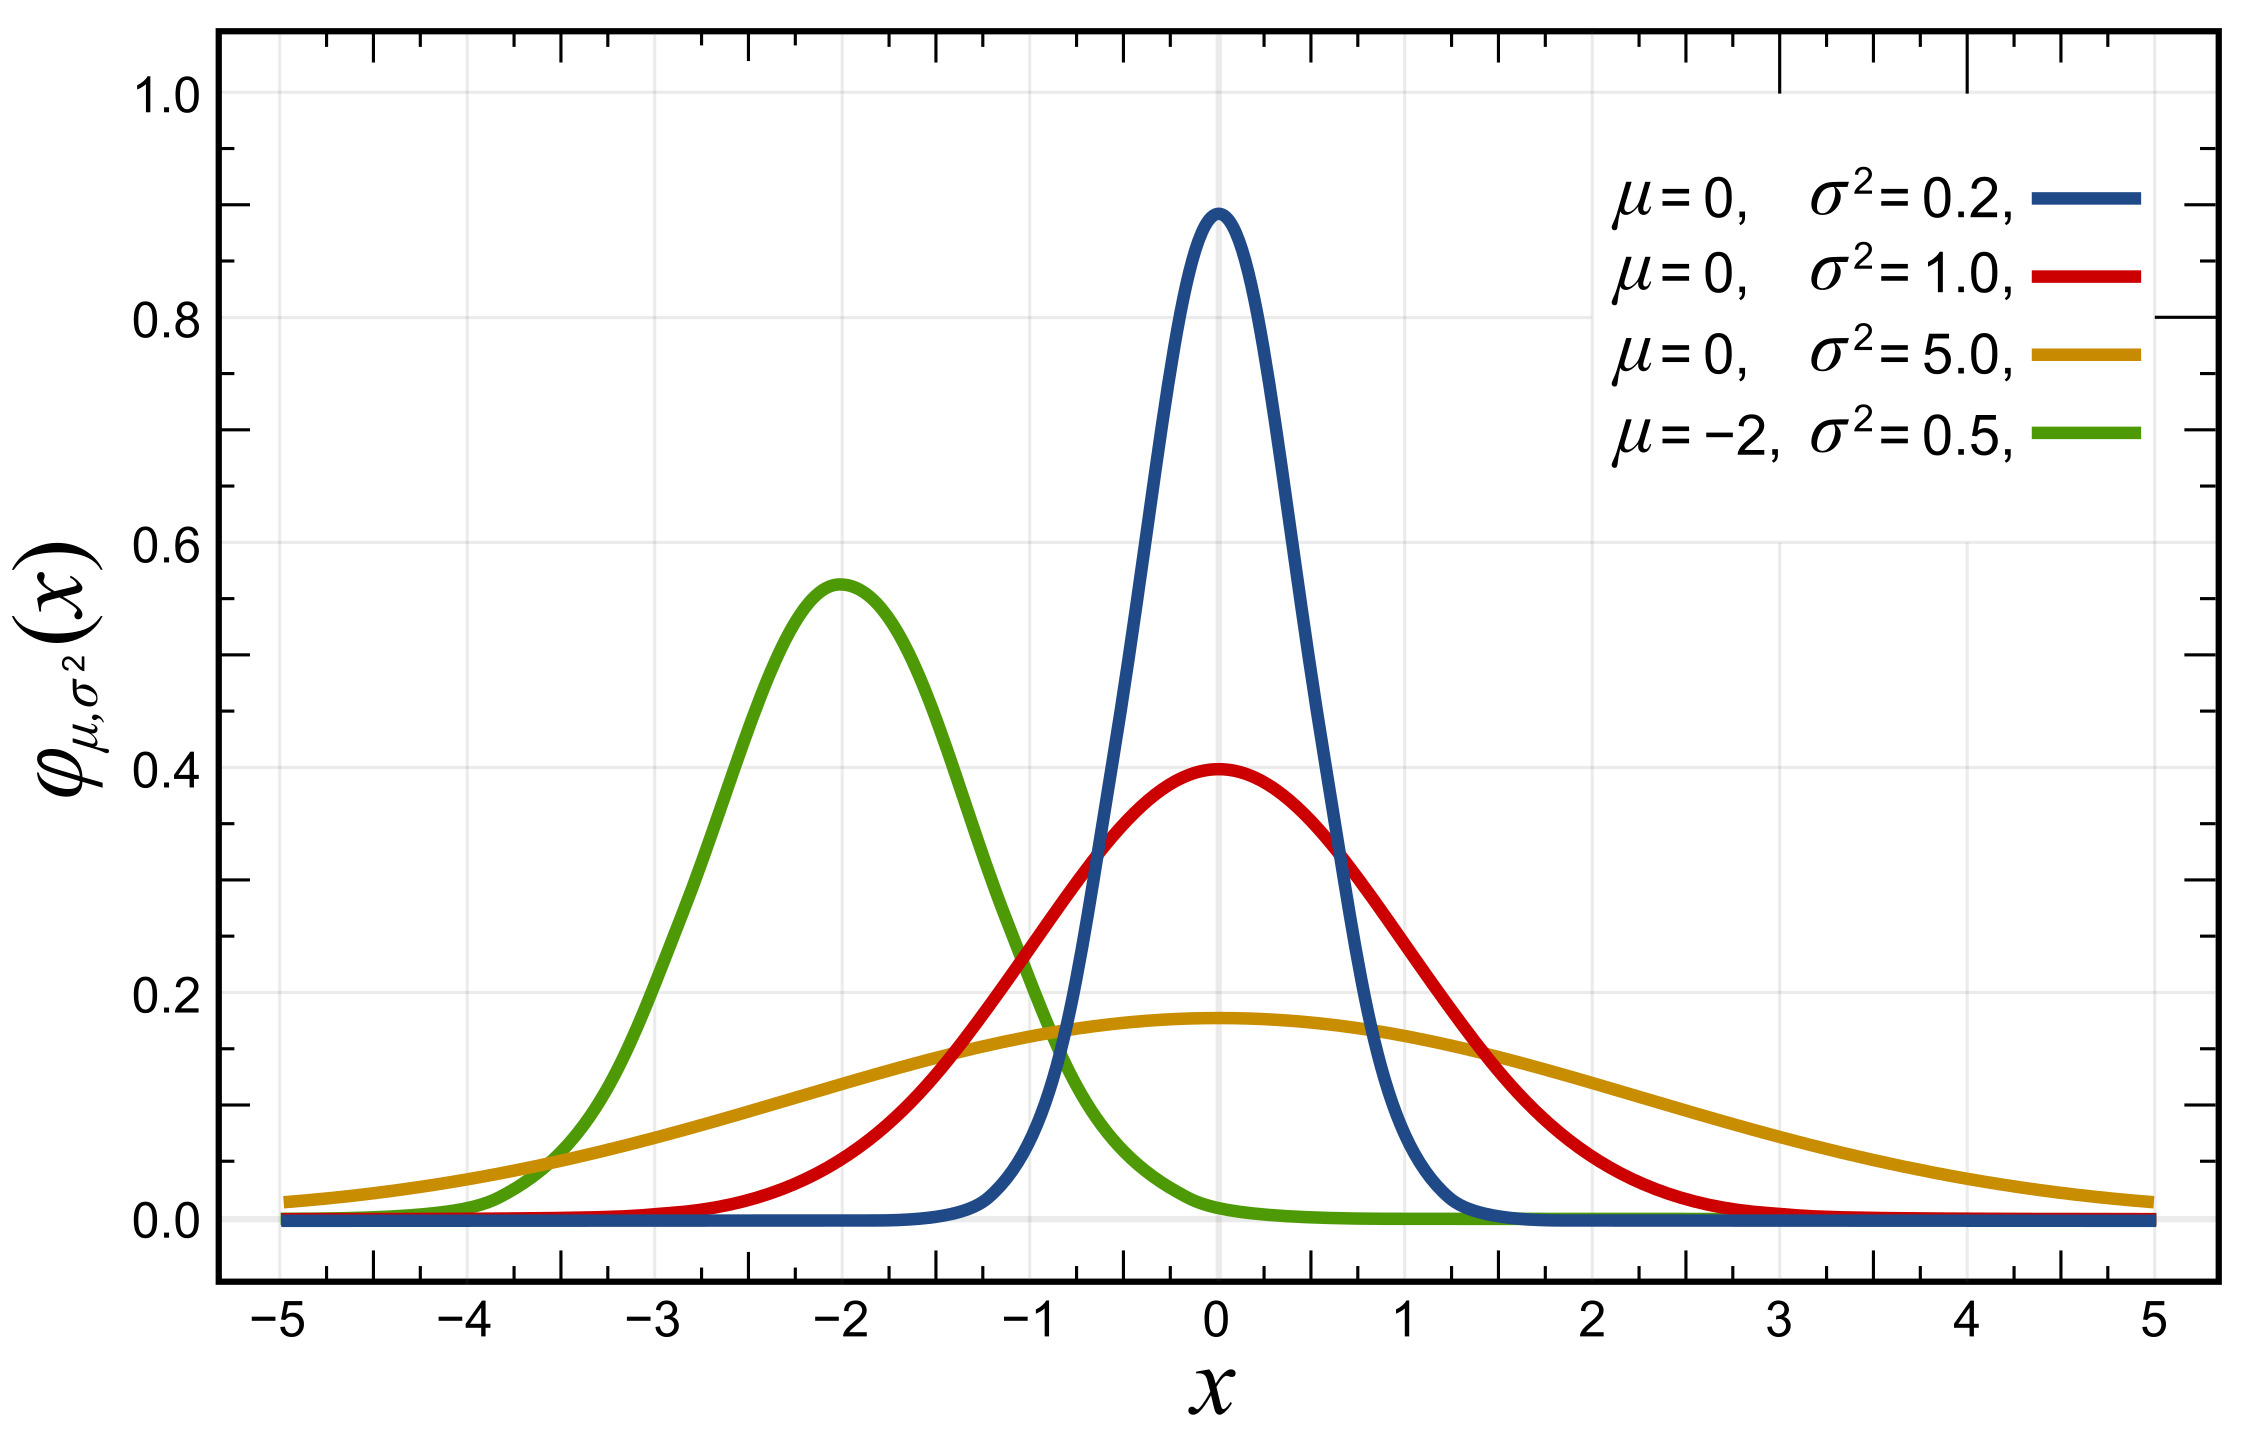
\includegraphics[width=\linewidth, height=4cm, keepaspectratio]{Pictures/distributions/Normal_Distribution_PDF.jpg}
            \caption{Normal distribution: PDF}
        \end{figure}
    \end{minipage}
    \hfill
    \begin{minipage}{0.49\linewidth}
        \begin{figure}[H]
            \centering
            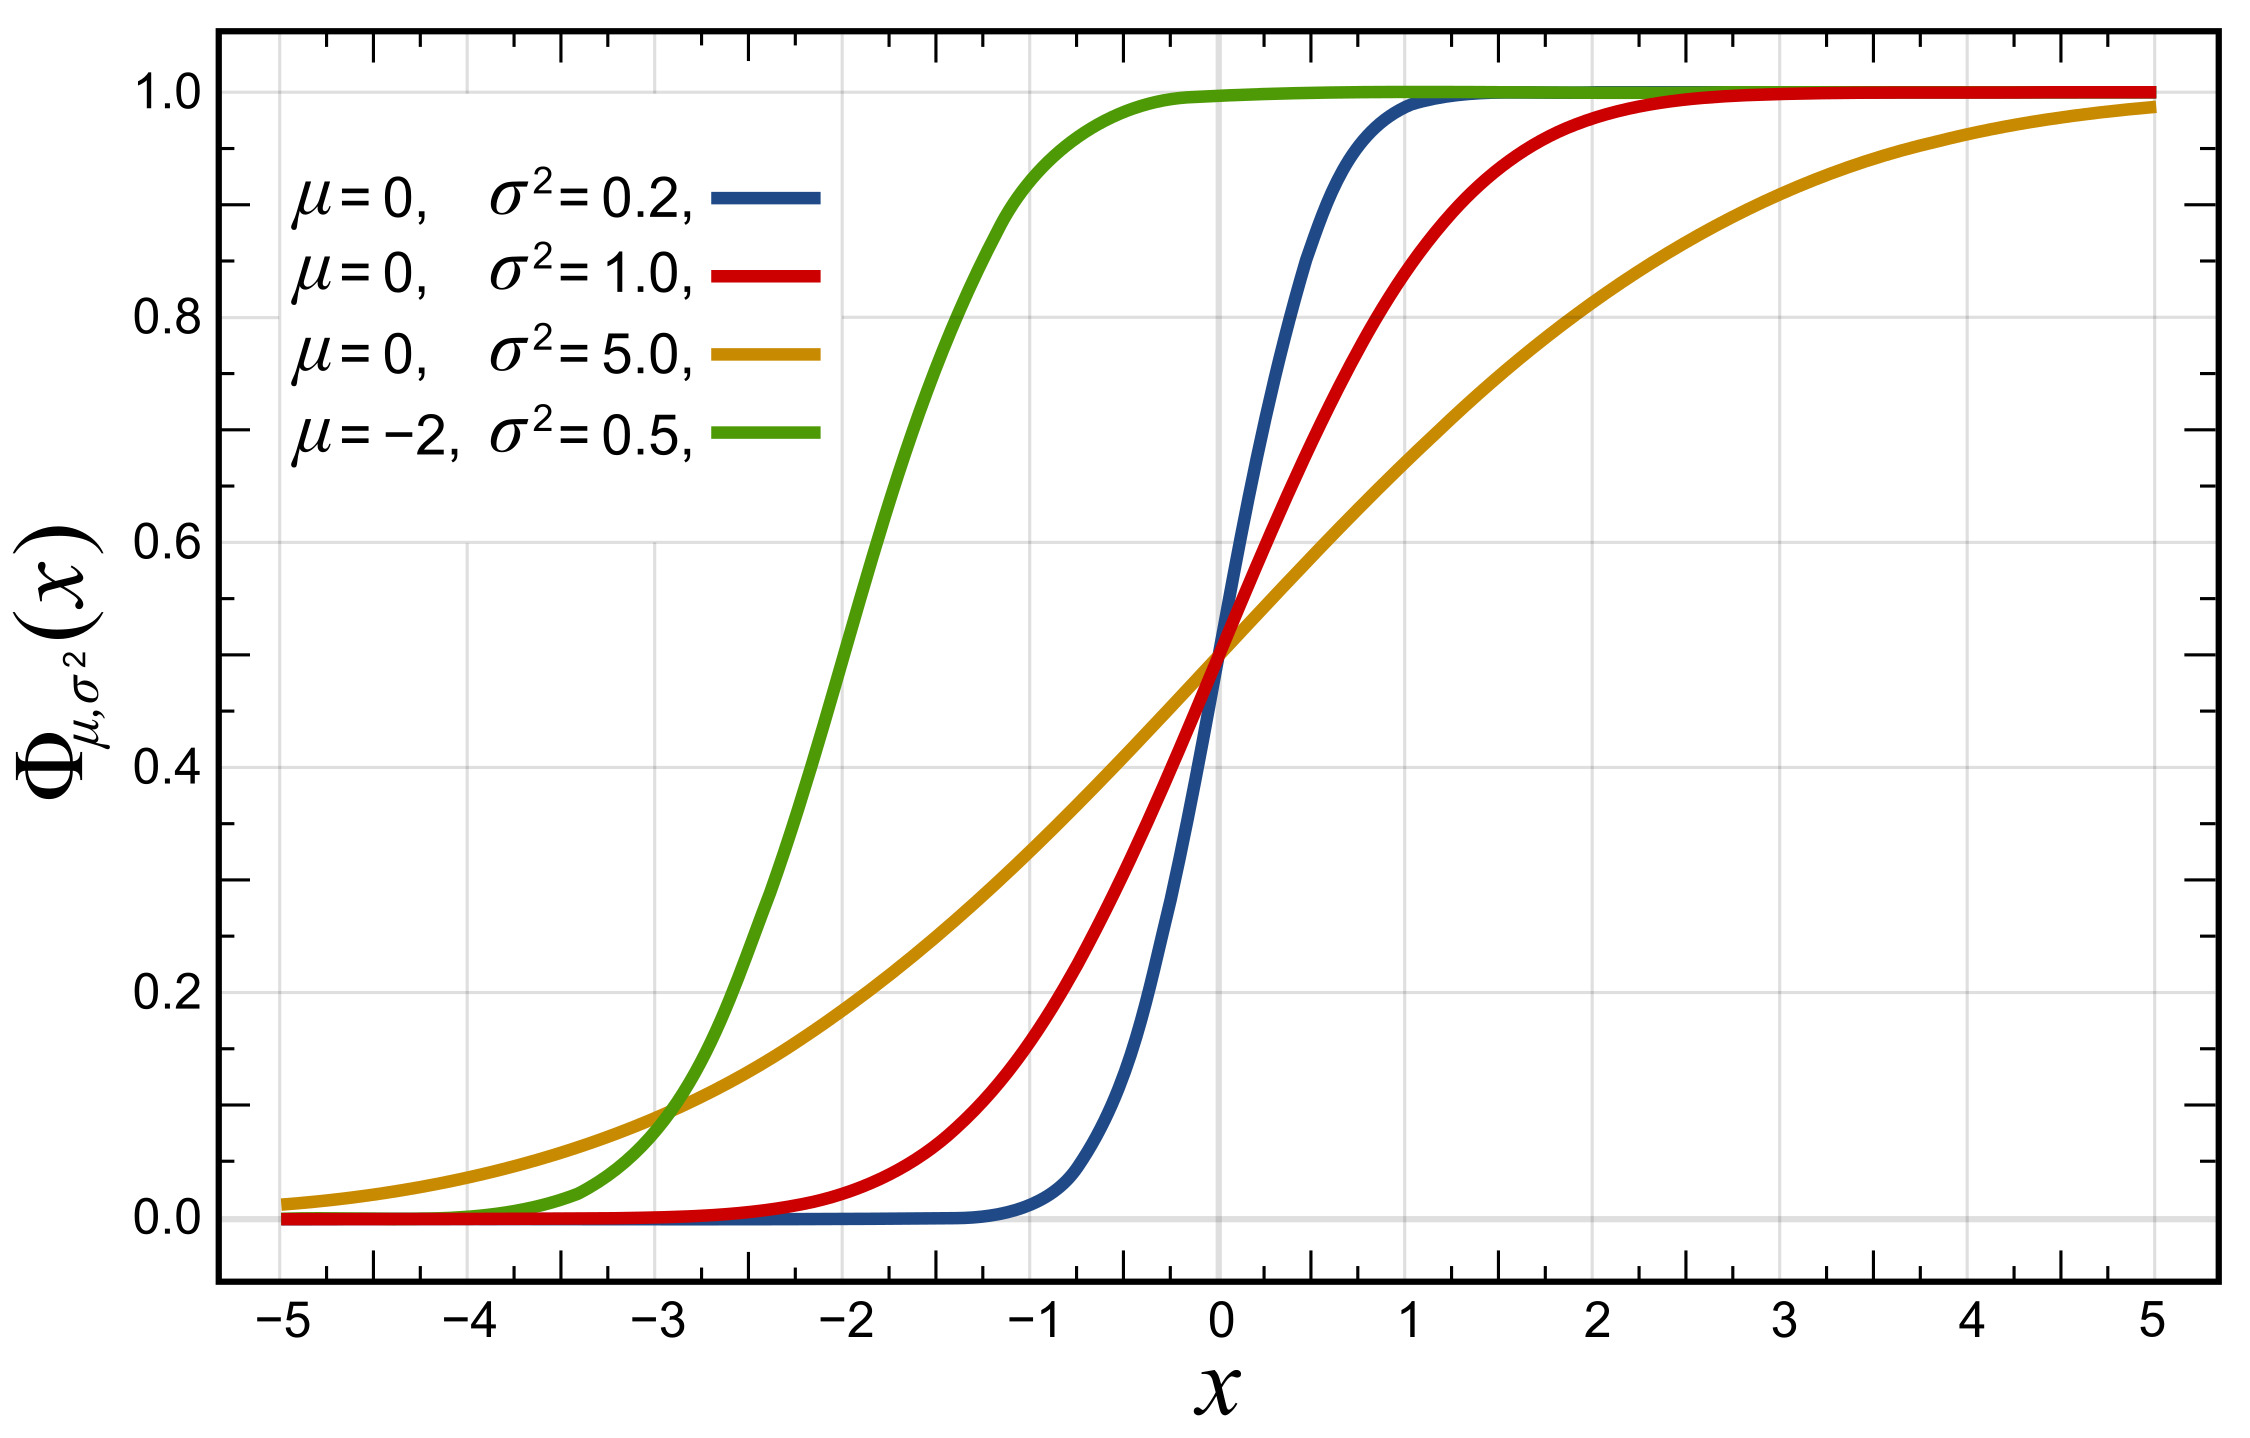
\includegraphics[width=\linewidth, height=4cm, keepaspectratio]{Pictures/distributions/Normal_Distribution_CDF.jpg}
            \caption{Normal distribution: CDF}
        \end{figure}
    \end{minipage}
\end{table}

\begin{customTableWrapper}{2}
\begin{longtable}{|m{6cm}|p{9cm}|}
    \hline
    \customTableHeaderColor
    \multicolumn{2}{|c|}{\textbf{Normal (Gaussian) Distribution/ Gauss curve - Info} \cite{wiki/Normal_distribution}} \\
    \hline\endfirsthead

    \hline
    \customTableHeaderColor
    \multicolumn{2}{|c|}{\textbf{Normal (Gaussian) Distribution/ Gauss curve - Info - contd.} \cite{wiki/Normal_distribution}} \\
    \hline\endhead
    
    \hline\endfoot
    \hline\endlastfoot

    \hline
    \textbf{Notation} & 
    ${\displaystyle {\mathcal {N}}(\mu ,\sigma ^{2})}$ 
    \\ \hline

    \textbf{Statistical parameters} & 
    \tableenumerate{
        \item ${\displaystyle \mu \in \mathbb {R} }$ = mean (location)
        
        \item ${\displaystyle \sigma ^{2}\in \mathbb {R} _{>0}}$ = variance (squared scale)
    }
    \\ \hline
    
    \textbf{Support} & 
    ${\displaystyle x\in \mathbb {R} }$
    \\ \hline

    \textbf{Probability Density Function (PDF)} & 
    $\vspace{0.1cm}{\displaystyle {\dfrac {1}{\sqrt {2\pi \sigma ^{2}}}}e^{-{\dfrac {(x-\mu )^{2}}{2\sigma ^{2}}}}}$
    \\[2ex] \hline
    
    \textbf{Cumulative distribution function (CDF)} & 
    ${\displaystyle \Phi \left({\dfrac {x-\mu }{\sigma }}\right)={\dfrac {1}{2}}\left[1+\operatorname {erf} \left({\dfrac {x-\mu }{\sigma {\sqrt {2}}}}\right)\right]}$
    \\ \hline

    \textbf{Quantile} &
    ${\displaystyle \mu +\sigma {\sqrt {2}}\operatorname {erf} ^{-1}(2p-1)}$
    \\ \hline

    \textbf{Mean} & 
    $\mu$
    \\ \hline

    \textbf{Median} & 
    $\mu$
    \\ \hline

    \textbf{Mode} & 
    $\mu$
    \\ \hline

    \textbf{Variance} &
    $\sigma^2$
    \\ \hline

    \textbf{Mean absolute deviation (MAD)} &
    ${\displaystyle \sigma {\sqrt {\dfrac{2}{\pi} }}}$ 
    \\[1ex] \hline

    \textbf{Skewness} &
    $0$ 
    \\ \hline

    \textbf{Excess kurtosis} &
    $0$ 
    \\ \hline

    \textbf{Entropy} &
    ${\displaystyle {\dfrac {1}{2}}\log(2\pi e\sigma ^{2})}$
    \\[1ex] \hline

    \textbf{Moment-generating function (MGF)} &
    ${\displaystyle \exp(\mu t+\dfrac{\sigma ^{2}t^{2}}{2})}$
    \\[1ex] \hline

    \textbf{Characteristic function (CF)} &
    ${\displaystyle \exp(i\mu t-\dfrac{\sigma ^{2}t^{2}}{2})}$
    \\[1ex] \hline

    \textbf{Fisher information} &
    \tableenumerate{
        \item ${\displaystyle {\mathcal {I}}(\mu ,\sigma )={\begin{pmatrix}1/\sigma ^{2}&0\\0&2/\sigma ^{2}\end{pmatrix}}}$
        \vspace{0.1cm}

        \item ${\displaystyle {\mathcal {I}}(\mu ,\sigma ^{2})={\begin{pmatrix}1/\sigma ^{2}&0\\0&1/(2\sigma ^{4})\end{pmatrix}}}$
        \vspace{0.1cm}
    }
    \\[1ex] \hline

    \textbf{Kullback–Leibler divergence} &
    ${\displaystyle {1 \over 2}\left\{\left({\frac {\sigma _{0}}{\sigma _{1}}}\right)^{2}+{\frac {(\mu _{1}-\mu _{0})^{2}}{\sigma _{1}^{2}}}-1+\ln {\sigma _{1}^{2} \over \sigma _{0}^{2}}\right\}}$
    \\[2ex] \hline

\end{longtable}
\end{customTableWrapper}












\begin{enumerate}
    \item First introduced explicitly as a PDF by Carl Friedrich Gauss, and it is therefore often referred to as the \textbf{Gauss curve} \indexlabel{Gauss curve}
\end{enumerate}

\section{Probability Density Function (PDF) ($f_{\mu,\sigma}(x)$ / $p(x|\mu,\sigma^2)$) \cite{ism-1,mfml-1}} \label{Normal Distribution: PDF}

\[
    p(x|\mu,\sigma^2)
    = f_{\mu,\sigma}(x)
    = \dfrac{1}{\sqrt{2\pi\sigma^2}}
    \exp\dParenBrac{
        -\dfrac{(x - \mu)^2}{2\sigma^2}
    }
    = \dfrac{1}{\sigma}\phi\dParenBrac{
        \dfrac{x - \mu}{\sigma}
    }
\]


\section{Cumulative Distribution Function (CDF) ($F_{\mu,\sigma}(x)$/ $\Phi\dParenBrac{ \frac{x-\mu}{\sigma} }$) \cite{ism-1}} \label{Normal Distribution: CDF}

\[
    \Phi\dParenBrac{\dfrac{x-\mu}{\sigma}}
    = F_{\mu,\sigma}(x)
    = Pr(X \leq x)
    = \dint_{-\infty}^x \dfrac{1}{\sigma}\phi\dParenBrac{
        \dfrac{z - \mu}{\sigma}
    } dz
    = \dint_{-\infty}^{(x - \mu)/\sigma} \phi(z) dz
\]
\[
    \Phi(x) = \dint_{-\infty}^{x} \phi(z) dz
\]


\section{Properties \cite{ism-1}}

\begin{enumerate}
    \item $z_p = -z_{1-p}$

    \item The sum of the random variables $\dsum_{i=1}^{n} X_i$ is again normally distributed, but now with mean $n\mu$ and variance $n\sigma^2$
\end{enumerate}

\section{Confidence Interval \cite{ism-1}}


\begin{enumerate}[itemsep=0.5cm]
    \item $\dfrac{\bar{X} - \mu}{\sigma/\sqrt{n}}$ is standard normal distributed

    \item $V_{n-1}^2 = (n-1)S^2/\sigma^2 \sim \chi_{n-1}^2$ is chi-square distributed

    \item $
        \dfrac{\bar{X} - \mu}{S/\sqrt{n}}
        = \dfrac{
            {(\bar{X} - \mu)}/{(\sigma/\sqrt{n})}
        }{
            \sqrt{(n-1)S^2/\sigma^2}/\sqrt{n-1}
        }
        =\dfrac{Z}{V_{n-1}/\sqrt{n-1}}
    $

    \item $\dfrac{\bar{X} - \mu}{S/\sqrt{n}}$ is student t distributed (DOF: $n-1$)

    \item Popular Confidence Intervals:
    \begin{table}[H]
        \centering
        \begin{tabular}{r l l}
            $95\%$ & $[\mu - 1.96\sigma,$ & $\mu + 1.96\sigma]$ \\
            
            $95.45\%$ &  $[\mu - 2\sigma,$ & $\mu + 2\sigma]$ \\

            $99.73\%$ & $[\mu - 3\sigma,$ & $\mu + 3\sigma]$ \\

        \end{tabular}
    \end{table}

\end{enumerate}

\section{Bivariate/ Multivariate \cite{ism-1,mfml-1}} \label{Normal distribution: Bivariate/ Multivariate}

\begin{table}[H]
    \centering
    \begin{tabular}{l l}
        $\rho$ & correlation coefficient\\
        
    \end{tabular}
\end{table}

if $\rho = 0$, $X \& Y$ are \textbf{independent}

\subsection{Probability Density Function (PDF) \cite{ism-1,mfml-1}} \label{Normal distribution: Bivariate/ Multivariate: PDF}

\begin{enumerate}[itemsep=0.5cm]
    \item $
        \hfill
        z_1 = \dfrac{x - \mu_X}{\sigma_X}
        \hfill
        z_2 = \dfrac{y - \mu_Y}{\sigma_Y}
        \hfill
    $ \hfill \cite{ism-1}
    
    \item $
        f(x,y)
        = \dfrac{1}{
            2\pi \sigma_X \sigma_Y \sqrt{1 - \rho^2}
        }
        \exp\left(
            -\dfrac{z_1^2 - 2\rho z_1z_2 + z_2^2}{2(1 - \rho^2)}
        \right)
    $ \hfill \cite{ism-1}

    \item $
        p(x|\mu, \Sigma)
        = (2\pi)^{-D/2} \dabs{\Sigma}^{-1/2}
        \exp(
            -0.5(x - \mu)^\top\Sigma^{-1}(x - \mu)
        )
        \hfill
        (x \in \mathbb{R}^D)
    $ \hfill \cite{mfml-1}

    \item marginal covariance matrix of $x$: $
        \Sigma_{xx} = Co\mathbb{V}[x,x]
    $

    \item marginal covariance matrix of $y$: $
        \Sigma_{yy} = Co\mathbb{V}[y,y]
    $

    \item cross-covariance matrix between x and y: $
        \Sigma_{xy} = \Sigma_{yx} = Co\mathbb{V}[x,y] = Co\mathbb{V}[y,x]
    $

    \item $
        p(x,y)
        = \mathcal{N}\left(
            \begin{bmatrix}
                \mu_x \\ \mu_y
            \end{bmatrix},
            \begin{bmatrix}
                \Sigma_{xx} & \Sigma_{xy} \\ 
                \Sigma_{yx} & \Sigma_{yy} \\ 
            \end{bmatrix}
        \right)
    $ \hfill \cite{mfml-1}
\end{enumerate}

\subsection{conditional distribution \cite{mfml-1}} \label{Normal distribution: Bivariate/ Multivariate: conditional distribution}

\begin{enumerate}[itemsep=0.3cm]
    \item $
        \mu_{x|y} 
        = \mu_x + \Sigma_{xy} \Sigma_{yy}^{-1} (y-\mu_y)
    $

    \item $
        \Sigma_{x|y}
        = \Sigma_{xx} - \Sigma_{xy} \Sigma_{yy}^{-1} \Sigma_{yx}
    $
    
    \item $
        p(x|y) = \mathcal{N}(\mu_{x|y}, \Sigma_{x|y})
    $

    \item in the computation of the mean, the $y$-value is an observation and no longer random
\end{enumerate}


\subsection{marginal distribution \cite{mfml-1}} \label{Normal distribution: Bivariate/ Multivariate: marginal distribution}

\begin{enumerate}[itemsep=0.3cm]
    \item $
        p(x)
        = \dint p(x,y)dy
        = \mathcal{N}(x|\mu_x, \Sigma_{xx})
    $

\end{enumerate}


\subsection{PDF of standardized random variables \cite{ism-1}} \label{Normal distribution: Bivariate/ Multivariate: PDF of standardized random variables}

\[
    \dfrac{
        \exp\{ 
            -(z_1^2 - 2\rho z_1 z_2 + z_2^2)/
            (2(1-\rho^2))
        \}
    }{
        \sqrt{2\pi(1-\rho^2)}
    }
\]


\subsection{Covariance ($COV(X,Y)$) \cite{ism-1}} \label{Normal distribution: Bivariate/ Multivariate: Covariance}

\[
\begin{aligned}
    COV(X,Y)
    &= \mathbb{E}(X - \mu_X)(Y - \mu_Y) \\
    &= \sigma_X \sigma_Y \mathbb{E}[Z_1Z_2] \\
    &= \sigma_X \sigma_Y \dint_{-\infty}^{\infty}
        \dint_{-\infty}^{\infty} 
        \dfrac{z_1 z_2}{2\pi (1 - \rho^2)}
        \exp\left\{ 
            -\dfrac{z_1^2 - 2\rho z_1 z_2 + z_2^2}{2(1-\rho^2)}
        \right\}
        dz_1 dz_2 \\
    &= \sigma_X \sigma_Y 
        \dint_{-\infty}^{\infty} \dfrac{z_2}{\sqrt{2\pi}}
        \exp \dCurlyBrac{- \dfrac{z_2^2}{2}}
        \dint_{-\infty}^{\infty}
        \dfrac{z_1}{\sqrt{2\pi(1-\rho^2)}}
        \exp \dCurlyBrac{ -\dfrac{(z_1 - \rho z_2)^2}{2(1- \rho^2)}} dz_1 dz_2 \\
    &= \sigma_X \sigma_Y \dint_{-\infty}^{\infty}
        \dfrac{\rho z_2^2}{\sqrt{2\pi}}
        \exp \dCurlyBrac{- \dfrac{z_2^2}{2}} d z_2 \\
    &= \rho \sigma_X \sigma_Y
\end{aligned}
\]


\subsection{Linear Combination of $X$ and $Y$ \cite{ism-1}} \label{Normal distribution: Bivariate/ Multivariate: linear combination}

\begin{table}[H]
    \centering
    \begin{tabular}{l l}
        Constants & $\alpha, \beta$ \\
    
        New random variable & $Z = \alpha X + \beta Y$ \\

        Mean & $\mu_Z = \alpha \mu_X + \beta \mu_Y$ \\

        Variance & $
            \sigma_Z^2 
            = \alpha^2 \sigma^2_X 
            + 2\alpha\beta\rho\sigma_X\sigma_Y 
            + \beta^2 \sigma^2_Y
        $ \\

    \end{tabular}

\end{table}


\subsection{Product of Gaussian Densities \cite{mfml-1}}\label{Product of Gaussian Densities}

\begin{enumerate}
    \item The product of two Gaussians 
    $\mathcal{N}(x|a, A) \mathcal{N}(x|b, B) = c_0\mathcal{N}(x|c, C)$
    \begin{enumerate}
        \item $C = (A^{-1} + B^{-1})^{-1}$

        \item $c = C(A^{-1}a + B^{-1}b)$

        \item $
            c_0 
            = (2\pi)^{-D/2}
            \dabs{A + B}^{-1/2}
            \exp(-0.5(a - b)^\top(A + B)^{-1}(a - b))
            \in \mathbb{R}
        $

    \end{enumerate}

    \item The \textbf{scaling constant} $c_0$ itself can be written in the form of a Gaussian density either in $a$ or in $b$ with an “inflated” covariance matrix $A + B$, i.e., $
        c_0 
        = \mathcal{N}(a|b, A + B) 
        = \mathcal{N}(b|a, A + B)
    $

\end{enumerate}


\subsection{Sums and Linear Transformations \cite{ism-1}} \label{Normal distribution: Bivariate/ Multivariate: Sums and Linear Transformations}

\begin{enumerate}
    \item If $X$, $Y$ are \textbf{independent} Gaussian random variables (i.e., the joint distribution is given as $p(x, y) = p(x)p(y))$ with $p(x) = \mathcal{N}(x|\mu_x , \Sigma_x)$ and $p(y) = \mathcal{N}(y|\mu_y , \Sigma_y)$, then $x + y$ is also Gaussian distributed and given by:
    \begin{enumerate}
        \item $p(x + y) = \mathcal{N}(\mu_x + \mu_y, \Sigma_x + \Sigma_y)$

        \item $p(ax + by) = \mathcal{N}(a\mu_x + b\mu_y , a2\Sigma_x + b2\Sigma_y)$
    \end{enumerate}
\end{enumerate}



\subsubsection{Linear Transformation}

Consider a Gaussian distributed random variable $X \sim \mathcal{N}(\mu , \Sigma )$. For a given matrix $A$ of appropriate shape, let $Y$ be a random variable such that $y = Ax$ is a transformed version of $x$.

\begin{table}[H]
    \begin{tabular}{l l}
        mean & $\mathbb{E}[y] = \mathbb{E}[Ax] = A\mathbb{E}[x] = A\mu $ \\

        variance & $\mathbb{V}[y] = \mathbb{V}[Ax] = A\mathbb{V}[x]A^\top  = A\Sigma A^\top $ \\

        PDF & $p(y) = \mathcal{N}(y|A\mu , A\Sigma A^\top )$ \\

    \end{tabular}
\end{table}


\subsubsection{Reverse Transformation}

We know that a random variable has a mean that is a linear transformation of another random variable. For a given full rank matrix $A \in R^{M\times N}$, where $M \geq N$, let $y \in RM$ be a Gaussian random variable with mean $Ax$, i.e., 

\begin{enumerate}[itemsep=0.3cm]
    \item $p(y) = \mathcal{N}(y|Ax, \Sigma )$

    \item $y = Ax \Leftrightarrow (A^\top A)^{-1} A^\top y = x$
\end{enumerate}

\begin{customTableWrapper}{1}
\begin{table}[H]
    \begin{tabular}{l l}
        PDF & $p(x) = \mathcal{N}(x|(A^\top A)^{-1} A^\top y, (A^\top A)^{-1} A^\top \Sigma A(A^\top A)^{-1} )$\\

        
    \end{tabular}
\end{table}
\end{customTableWrapper}


\subsubsection{Pearson’s correlation coefficient ($\rho_P$) \cite{ism-1}} \label{Normal distribution: Bivariate/ Multivariate: Pearson’s correlation coefficient}

\[
    \rho_P
    = CORR(X,Y)
    = \rho
\]

\subsubsection{Estimation of Pearson’s correlation coefficient ($r_P$) \cite{ism-1}} \label{Normal distribution: Bivariate/ Multivariate: Estimation of Pearson’s correlation coefficient}

TODO

\subsubsection{Kendall’s tau correlation coefficient ($\tau_K$) \cite{ism-1}} \label{Normal distribution: Bivariate/ Multivariate: Kendall’s tau correlation coefficient}

\[
    \tau_K = \dfrac{2 arcsin(\rho)}{\pi}
\]

\subsubsection{Spearman’s rho correlation coefficient ($\rho_S$) \cite{ism-1}} \label{Normal distribution: Bivariate/ Multivariate: Spearman’s rho correlation coefficient}

\[
    \rho_S = \dfrac{2}{\pi} arcsin\dParenBrac{\dfrac{\rho}{2}}
\]

\subsubsection{Estimation of Spearman’s rho correlation coefficient \cite{ism-1}} \label{Normal distribution: Bivariate/ Multivariate: Estimation of Spearman’s rho correlation coefficient}

\[
\begin{aligned}
    Pr(R^X_n = n) 
    &= Pr(X_n = \max\dCurlyBrac{X_1, X_2,\cdots , X_n}) \\
    &= Pr(X_n \geq X_1, X_n \geq X_2,\cdots , X_n \geq X_{n-1}) \\
    &= \dint_{-\infty}^{\infty}
        Pr(X_n \geq X_1, X_n \geq X_2,\cdots, X_n \geq X_{n-1}|X_n = x) f_{X_n}(x)dx \\
    &= \dint_{-\infty}^{\infty}
        Pr(X_1 \leq x, X_2 \leq x,\cdots, X_{n-1} \leq x|X_n = x) f_{X_n}(x)dx \\
    &= \dint_{-\infty}^{\infty} F^{n-1}_X (x) f_{X_n}(x)dx
\end{aligned}
\]

with $f_{X_n} = f_X$, since $X_1, X_2,\cdots, X_n$ are i.i.d. with CDF $F_X$

\begin{customTableWrapper}{2}
\begin{table}[H]
    \begin{tabular}{l l}
        mean & $
            \rho_S 
            = \mathbb{E}(r_S)
            = \dfrac{6}{(n+1)\pi}
                (arcsin(\rho) + 
                (n - 2) arcsin\dParenBrac{\dfrac{\rho}{2}})
            \approx \dfrac{6}{\pi} arcsin\dParenBrac{\dfrac{\rho}{2}})
        $ \\

        variance & $
            VAR(r_S)
            \approx \dfrac{1}{n} 
                (1 - 1.1563465\rho^{2} + 0.304743\rho^{4} + 0.155286\rho^{6})
        $ \\

        estimator of $\rho$ & $
            \hat{\rho} = 2\sin\dParenBrac{\dfrac{\pi r_S}{6} }
        $ \\

        
    \end{tabular}
\end{table}
\end{customTableWrapper}

\paragraph{Confidence Interval}

\begin{enumerate}[itemsep=0.2cm]
    \item using asymptotic confidence interval on $r_S$
    \begin{enumerate}[itemsep=0.2cm]
        \item coverage of the interval is often lower than $100(1 - \alpha)\%$

    \end{enumerate}
    
    \item confidence interval based on the $t$-distribution
    \begin{enumerate}[itemsep=0.2cm]
        \item coverage is typically larger than $100(1 - \alpha)\%$
    \end{enumerate}

    \item confidence intervals based on the Fisher z-transformation
    \begin{enumerate}[itemsep=0.2cm]
        \item close to $100(1 - \alpha)\%$
        
        \item Fisher z-transformation of $r_S$ uses normal confidence intervals with a variance $S_{r_S}^2$ of $r_S$ in this transformed scale
        \begin{enumerate}[itemsep=0.2cm]
            \item $
                S_{r_S}^2 
                = \dfrac{1.06}{n-3}
            $ \hfill (Fieller and Pearson 1961)

            \item $
                S_{r_S}^2 
                = \dfrac{1 + r_S^2/2}{n-3}
            $ \hfill (Bonett and Wright 2000)

            \item $
                S_{r_S}^2 
                = (n-2)^{-1} + \dfrac{\dabs{z_{r_S}}}{6n + 4\sqrt{n}}
            $ \hfill (Caruso and Cliff 1997)

        \end{enumerate}

        \item Fisher z-transformation of $r_S$
        \begin{enumerate}[itemsep=0.2cm]
            \item $z_{r_S} = 0.5[\log(1 + r_S) - \log(1 - r_S)]$

            \item Confidence Interval:
            $(
                z_{r_S} - z_{1 - \alpha/2}S_{r_S},
                z_{r_S} + z_{1 - \alpha/2}S_{r_S}
            ]$
        \end{enumerate}

        \item Original Scale
        \begin{enumerate}[itemsep=0.2cm]
            \item Confidence Interval:
            $\left(
                \dfrac{
                    \exp(2[z_{r_S} - z_{1 - \alpha/2}S_{r_S}]) - 1
                }{
                    \exp(2[z_{r_S} - z_{1 - \alpha/2}S_{r_S}]) + 1
                },
                \dfrac{
                    \exp(2[z_{r_S} + z_{1 - \alpha/2}S_{r_S}]) - 1
                }{
                    \exp(2[z_{r_S} + z_{1 - \alpha/2}S_{r_S}]) + 1
                }
            \right]$
        \end{enumerate}

    \end{enumerate}

    \item For correlation coefficients $\leq 0.5$, simulation studies with normally distributed random variables show that the Fisher z-transformed confidence intervals with the three different standard errors behave very similarly.

    \item When the correlation coefficient is larger than $0.5$, Fieller and Pearson’s standard error underestimates the variability of the estimator of Spearman’s rho. 

    \item For correlation coefficients larger than $0.7$, the standard error of Caruso and Cliff also starts to underestimate the variability of the estimator of Spearman’s rho.

    \item For the standard error of the approach of Bonett and Wright underestimation occurs for correlation coefficients larger than $0.9$
\end{enumerate}


\subsubsection{Sums of Random Variables \cite{ism-1}} \label{Normal distribution: Bivariate/ Multivariate: Sums of Random Variables}

\begin{enumerate}[itemsep=0.2cm]
    \item $
        \hfill
        U \sim \mathcal{N}(\mu_U, \sigma_U^2)
        \hfill
        V \sim \mathcal{N}(\mu_V, \sigma_V^2)
        \hfill
        W \sim \mathcal{N}(\mu_W, \sigma_W^2)
        \hfill
    $ such that:
    \begin{enumerate}
        \item $X = U + W$
        \item $Y = V + W$
    \end{enumerate}

\end{enumerate}

\renewcommand{\arraystretch}{2}
\begin{table}[H]
    \begin{tabular}{l l l}
        Mean & $\mu_X = \mu_U + \mu_W $ & $ \mu_Y = \mu_V + \mu_W$ \\

        Variance & $\sigma^2_X = \sigma^2_U + \sigma^2_W $ & $ \sigma^2_Y = \sigma^2_V + \sigma^2_W$ \\

        Correlation coefficient & $
            \rho = \dfrac{\sigma_W^2}{
                \sqrt{(\sigma^2_U + \sigma^2_W)(\sigma^2_V + \sigma^2_W)}
            }
        $ & \\
    \end{tabular}
\end{table}
\renewcommand{\arraystretch}{1}


\subsubsection{Mixture Distribution \cite{ism-1}} \label{Normal distribution: Bivariate/ Multivariate: Mixture Distribution}

\begin{enumerate}
    \item $
        \hfill
        f_{X|Z}(x|z) = \dfrac{1}{\sigma_1}
        \phi\dParenBrac{\dfrac{x-\mu_1-z}{\sigma_1} }
        \hfill
        f_{Y|Z}(y|z) = \dfrac{1}{\sigma_2}
        \phi\dParenBrac{\dfrac{y-\mu_2-z}{\sigma_2} }
        \hfill
    $ \cite{ism-1}

    
\end{enumerate}

\begin{table}[H]
    \centering
    \begin{tabular}{l l l}
        Mean & $\mu_X = \mu_Z + \mu_1$ & $\mu_Y = \mu_Z + \mu_2$ \\

        Variance & $\sigma^2_X = \sigma^2_Z + \sigma^2_1$ & $\sigma^2_Y = \sigma^2_Z + \sigma^2_2$ \\

        dependency parameter & $
            \rho
            = \dfrac{\sigma^2_Z}{
                \sqrt{(\sigma^2_Z + \sigma^2_1)(\sigma^2_Z + \sigma^2_2)}
            }
        $
    \end{tabular}
\end{table}

\begin{theorem}
    Consider a mixture of two univariate Gaussian densities \cite{mfml-1}
    \[
        p(x) = \alpha p_1(x) + (1 - \alpha )p_2(x)    
        \hfill
        (0 < \alpha  < 1)
    \]
    \begin{enumerate}
        \item $\alpha$ : mixture weight
        
        \item $p_1(x)$ and $p_2(x)$ are univariate Gaussian densities with different parameters, i.e., 
        \[
            (\mu_1 , \sigma_1^2) \neq (\mu_2 , \sigma_2^2)
        \]
        
        \item Mean  : $\mathbb{E}[x] = \alpha \mu_1 + (1 - \alpha )\mu_2$
        
        \item Variance : $\mathbb{V}[x] = [\alpha \sigma_1^2 + (1-\alpha )\sigma_2^2] + ([\alpha \mu_1^2 + (1-\alpha )\mu_2^2] - [\alpha \mu_1 + (1-\alpha )\mu_2]^2)$

    \end{enumerate}

\end{theorem}

\subsubsection{Bayesian analysis \cite{ism-1}} \label{Normal distribution: Bivariate/ Multivariate: Bayesian analysis}

\begin{enumerate}
    \item $X_1, \cdots, X_n$ are i.i.d. $\mathcal{N} (\mu, \sigma^2)$

    \item $f(\theta|D) = f(\mu, \sigma^2|D)$
\end{enumerate}

\paragraph{Bayesian Analysis for Normal Populations Based on Single Observation \cite{ism-1}} \label{Bayesian Analysis for Normal Populations Based on Single Observation}

\begin{enumerate}[itemsep=0.2cm]
    \item $\sigma^2$ is known
    \begin{enumerate}[itemsep=0.2cm]
        \item $
            l(\theta) 
            = p(x|\mu)
            =\dfrac{1}{\sqrt{2\pi \sigma^2}}
            \exp\left(
                -\dfrac{(x-\mu)^2}{2\sigma^2}
            \right)
        $

        \item $
            f(\mu) 
            = p(x|\mu)
            =\dfrac{1}{\sqrt{2\pi \sigma^2_0}}
            \exp\left(
                -\dfrac{(\mu-\mu_0)^2}{2\sigma_0^2}
            \right)
        $

        \item posterior:
        \[
        \begin{aligned}
            f(\mu|x)
            &\propto p(x|\mu)f(\mu) \\
            &=\dfrac{1}{\sqrt{2\pi \sigma^2}}
            \exp\left(
                -\dfrac{(x-\mu)^2}{2\sigma^2}
            \right) 
            \times 
            \dfrac{1}{\sqrt{2\pi \sigma^2_0}}
            \exp\left(
                -\dfrac{(\mu-\mu_0)^2}{2\sigma_0^2}
            \right) \\
            &=\dfrac{1}{2\pi \sigma\sigma_0}
            \exp\left(
                -\dfrac{(x-\mu)^2}{2\sigma^2}
                -\dfrac{(\mu-\mu_0)^2}{2\sigma_0^2}
            \right) \\
            &\propto
            \exp\left\{
                \dfrac{
                    -\dParenBrac{\mu - \dfrac{\mu_0\sigma^2 + x\sigma_0^2}{\sigma^2 + \sigma^2_0}}^2
                }{
                    2\dParenBrac{ \dfrac{\sigma^2\sigma^2_0}{\sigma^2+\sigma^2_0} }
                }
            \right\}
        \end{aligned}
        \]

        \item $
            \sigma_1^2
            = \dfrac{\sigma^2\sigma^2_0}{\sigma^2+\sigma^2_0}
            = \dfrac{1}{\sigma^{-2}+\sigma^{-2}_0}
        $ \\[2ex]
        $
            \Rightarrow
            \sigma_1^{-2} = \sigma^{-2}+\sigma^{-2}_0
        $

        \item $
            \mu_1
            =  \dfrac{\mu_0\sigma^2 + x\sigma_0^2}{\sigma^2 + \sigma^2_0}
            =  \dfrac{\mu_0\sigma^{-2} + x\sigma_0^{-2}}{\sigma^{-2} + \sigma^{-2}_0}
            = \sigma_1^2(\mu_0\sigma^{-2} + x\sigma_0^{-2})
        $ \\[2ex]
        $
            \Rightarrow
            \mu_1\sigma_1^{-2} = \mu_0\sigma^{-2} + x\sigma_0^{-2}
        $

        \item $
            f(\mu|x) 
            = \dfrac{1}{\sqrt{2\pi\sigma_1^2}} \exp\left(
                \dfrac{(\mu - \mu_1)^2}{2\sigma^2}
            \right)
        $

        \item posterior for $\mu$ is itself a Normal: $\mu|X_1 = x \sim \mathcal{N} (\mu_1, \sigma_1^2)$
    \end{enumerate}

\end{enumerate}

\paragraph{Bayesian Analysis for Normal Populations Based on Multiple Observations \cite{ism-1}} \label{Bayesian Analysis for Normal Populations Based on Multiple Observations}

set of realizations : $x_1, \cdots, x_n$

\begin{enumerate}[itemsep=0.2cm]
    \item $\sigma^2$ known \cite{ism-1}
    \begin{enumerate}[itemsep=0.2cm]
        \item likelihood: 
        \[
        \begin{aligned}
            l(\theta)
            &= p(x_1, \cdots, x_n|\mu) \\
            &= \dprod_{i=1}^{n} 
                \dfrac{1}{\sqrt{2\pi\sigma^2}}
                \exp\dParenBrac{
                    -\dfrac{(x_i - \mu)^2}{2\sigma^2}
                }
        \end{aligned}
        \]

        \item $
            f(\mu|x_1, \cdots, x_n) 
            = \dfrac{1}{\sqrt{2\pi\sigma_1^2}}
                \exp\dParenBrac{
                    \dfrac{(\mu - \mu_1)^2}{2\sigma^2}
                }
        $
        \begin{enumerate}[itemsep=0.2cm]
            \item $
                \sigma_1^2
                = \dParenBrac{
                    \dfrac{1}{\sigma_0^2} +
                    \dfrac{1}{\sigma^2/n}
                }^2
            $

            \item $
                \mu_1
                = \sigma_1^2\dParenBrac{
                    \dfrac{\mu_0}{\sigma_0^2} +
                    \dfrac{\bar{x}}{\sigma^2/n}
                }
            $
        \end{enumerate}

        \item If $n \to \infty$, then $\mu_1$ will converge to the sample mean, and $\sigma_1^2$ will converge to \textbf{zero}.
        
    \end{enumerate}

    \item Unknown Mean and Variance \cite{ism-1}
    \begin{enumerate}[itemsep=0.2cm]
        \item $\begin{aligned}
            l(\theta)
            &= p(x_1, \cdots, x_n|\mu, \sigma^2) \\
            &= \dprod_{i=1}^{n} 
                \dfrac{1}{\sqrt{2\pi\sigma^2}}
                \exp\dParenBrac{
                    -\dfrac{(x_i - \mu)^2}{2\sigma^2}
                }
        \end{aligned}$

        \item prior: Normal-inverse-$\chi^2$ distribution

        \renewcommand{\arraystretch}{2}
        \[
        \begin{aligned}
            f(\mu,\sigma)
            &= NI\chi^2(\mu_0, \kappa_0, \nu_0, \sigma_0^2) \\
            &= p(\mu,\sigma^2) = p(\mu|\sigma^2)p(\sigma^2)
            \\
            &= \mathcal{N}(\mu_0, \sigma^2/\kappa) \times
                \chi^{-2}(\nu_0, \sigma_0^2)\\
            &= \dfrac{
                (\sigma^2)^{-({\nu_0/2+1})/{2}}
            }{
                Z(\mu_0, \kappa_0, \nu_0, \sigma_0^2)
            } 
            \exp\dParenBrac{
                -\dfrac{\nu_0\sigma_0^2 + \kappa_0(\mu_0-\mu)^2}{2\sigma^2}
            }
        \end{aligned}
        \]
        \renewcommand{\arraystretch}{1}
        uses Scaled inverse chi square distribution
        \[
            Z(\mu_0, \kappa_0, \nu_0, \sigma_0^2)
            = \sqrt{\dfrac{2\pi}{\kappa_0}} 
            \Gamma\dParenBrac{\dfrac{\nu_0}{2}}
            \dParenBrac{\dfrac{2}{\nu_0\sigma_0^2}}
            ^{\dParenBrac{\dfrac{\nu_0}/{2}}}
        \]

        \item posterior: Normal-inverse-$\chi^2$ distribution
        \begin{enumerate}[itemsep=0.2cm]
            \item $
                f(\mu,\sigma|x_1,\cdots,x_n)
                = NI\chi^2(\mu_n, \kappa_n, \nu_n, \sigma_n^2) 
            $

            \item $
                \hfill
                \mu_n = \dfrac{\kappa_0\mu_0+n\bar{x}}{\kappa_n}
                \hfill
                \kappa_n = \kappa_0 + n
                \hfill
                \nu_n = \nu_0 + n
                \hfill
            $
            \[
                \hfill
                \sigma_n^2 = \dfrac{1}{\nu_n}
                \dParenBrac{
                    \nu_0\sigma_0^2
                    +\dsum_{i=1}^n (x_i-\bar{x})^2
                    +\dfrac{n\kappa_0}{\kappa_0 + n}
                    (\mu_0 + \bar{x})^2
                }
                \hfill
            \]

            \item $
                f(\sigma^2|x_1,\cdots,x_n) = \chi^{-2}(\nu_n, \sigma_n^2)
            $ \\[2ex]
            uses Scaled inverse chi square distribution \\
            \textbf{scale} = $\nu_n$ \& 
            \textbf{degrees of freedom} = $\sigma_n^2$

            \item $
                f(\mu|x_1,\cdots,x_n) 
                = t(\mu_n,\sigma_n^2/\kappa_n)
            $ \\[2ex]
            \textbf{mean} = $\mu_n$   \& 
            \textbf{degrees of freedom} = $\sigma_n^2/\kappa_n$

        \end{enumerate}

    \end{enumerate}

\end{enumerate}


\subsubsection{Exponential Family \cite{mfml-1}} \label{Normal distribution: Bivariate/ Multivariate: Exponential Family}

\begin{enumerate}
    \item Consider the univariate Gaussian distribution $\mathcal{N}(\mu, \sigma^2)$
    
    \item $\phi(x) = \begin{bmatrix} x & x^2 \end{bmatrix}^\top$

    \item $p(x | \theta) \propto \exp(\theta_1x + \theta_2x^2)$\\[1ex]
    setting $\theta = \begin{bmatrix}
        \dfrac{\mu}{\sigma^2} &
        -\dfrac{1}{2\sigma^2}
    \end{bmatrix}^\top$ and substituting, we obtain
    \[
        p(x|\theta)
        \propto \exp\dParenBrac{
            \dfrac{\mu x}{\sigma^2}
            -\dfrac{x^2}{2\sigma^2}
        } 
        \propto \exp\dParenBrac{
            -\dfrac{\dParenBrac{x - \mu}^2}{2\sigma^2}
        } 
    \]
    

\end{enumerate}


\section{Standard Normal Distribution ($X \sim \mathcal{N}(0,1)$/ $\mathcal{N}(0, I)$) \cite{ism-1,mfml-1}} \label{Standard Normal Distribution}

\begin{enumerate}
    \item Normal Distribution with: \\
    $
        \hfill
        \mu = 0
        \hfill
        \sigma = 1
        \hfill
        x \in \mathbb{R}
    $
\end{enumerate}


\subsection{Probability Density Function (PDF) ($\phi(x)$) \cite{ism-1}} \label{Standard Normal Distribution: PDF}

\[
    \phi(x)
    = \dfrac{1}{\sqrt{2\pi}}\exp\dParenBrac{-\dfrac{x^2}{2}}
\]


\subsection{Sampling from Multivariate Standard Normal Distribution \cite{mfml-1}} \label{Sampling from Multivariate Standard Normal Distribution}

\begin{enumerate}
    \item To obtain samples from a multivariate normal $\mathcal{N} (\mu , \Sigma )$, we can use the properties of a linear transformation of a Gaussian random variable: \\
    If $x \sim \mathcal{N} (0, I)$, then $y = Ax + \mu $, where $AA^\top  = \Sigma $ is Gaussian distributed with mean $\mu $ and covariance matrix $\Sigma $. One convenient choice of $A$ is to use the Cholesky decomposition of the covariance matrix $\Sigma  = AA^\top $. The Cholesky decomposition has the benefit that $A$ is triangular, leading to efficient computation.
\end{enumerate}

































\chapter{Lognormal Distribution ($X \sim \mathcal{LN}(\mu, \sigma^2)$) \cite{ism-1,wiki/Log-normal_distribution}} \label{Lognormal Distribution}

\begin{table}[H]
    \begin{minipage}{0.49\linewidth}
        \begin{figure}[H]
            \centering
            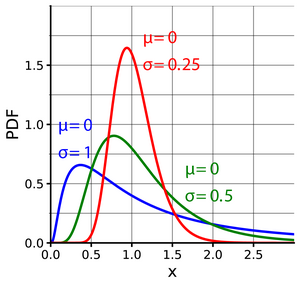
\includegraphics[width=\linewidth, height=4cm, keepaspectratio]{Pictures/distributions/Log-normal-pdfs.png}
            \caption{Lognormal distribution: PDF}
        \end{figure}
    \end{minipage}
    \hfill
    \begin{minipage}{0.49\linewidth}
        \begin{figure}[H]
            \centering
            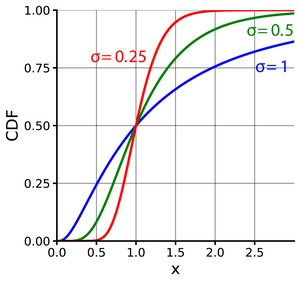
\includegraphics[width=\linewidth, height=4cm, keepaspectratio]{Pictures/distributions/Log-normal-cdfs.png}
            \caption{Lognormal distribution: CDF}
        \end{figure}
    \end{minipage}
\end{table}


\begin{alternateColorTable}
\renewcommand{\arraystretch}{2}
\begin{longtable}{|m{6cm}|p{9cm}|}
    \hline
    \tableHeaderRow
    \multicolumn{2}{|c|}{\textbf{Lognormal Distribution - Info} \cite{wiki/Log-normal_distribution}} \\
    \hline\endfirsthead

    \hline
    \tableHeaderRow
    \multicolumn{2}{|c|}{\textbf{Lognormal Distribution - Info - contd.} \cite{wiki/Log-normal_distribution}} \\
    \hline\endhead
    
    \hline\endfoot
    \hline\endlastfoot

    \hline
    \textbf{Notation} & 
    ${\displaystyle \ \operatorname {Lognormal} \left(\ \mu ,\,\sigma ^{2}\ \right)\ }$
    \\ \hline

    \textbf{Statistical parameters} & 
    \tableenumerate{
        \item ${\displaystyle \ \mu \in (\ -\infty ,+\infty \ )\ }$ (logarithm of location)

        \item ${\displaystyle \ \sigma >0\ }$ (logarithm of scale)
    }
    \\ \hline
    
    \textbf{Support} & 
    ${\displaystyle \ x\in (\ 0,+\infty \ )\ }$
    \\ \hline

    \textbf{Probability Density Function (PDF)} & 
    ${\displaystyle \ {\frac {1}{\ x\sigma {\sqrt {2\pi \ }}\ }}\ \exp \left(-{\frac {\left(\ln x-\mu \ \right)^{2}}{2\sigma ^{2}}}\right)}$
    \\[2ex] \hline
    
    \textbf{Cumulative distribution function (CDF)} & 
    ${\displaystyle \ {\frac {\ 1\ }{2}}\left[1+\operatorname {erf} \left({\frac {\ \ln x-\mu \ }{\sigma {\sqrt {2\ }}}}\right)\right]=\Phi \left({\frac {\ln(x)-\mu }{\sigma }}\right)}$
    \\ \hline

    \textbf{Quantile} &
    ${\displaystyle \ \exp \left(\mu +{\sqrt {2\sigma ^{2}}}\operatorname {erf} ^{-1}(2p-1)\right)\ }$
    \\ \hline

    \textbf{Mean} &
    ${\displaystyle \ \exp \left(\ \mu +{\frac {\sigma ^{2}}{2}}\ \right)\ }$
    \\ \hline

    \textbf{Median} & 
    ${\displaystyle \ \exp(\ \mu \ )\ }$
    \\ \hline

    \textbf{Mode} & 
    ${\displaystyle \ \exp \left(\ \mu -\sigma ^{2}\ \right)\ }$
    \\ \hline

    \textbf{Variance} &
    ${\displaystyle \ \left[\ \exp(\sigma ^{2})-1\ \right]\ \exp \left(2\ \mu +\sigma ^{2}\right)\ }$
    \\ \hline

    \textbf{Skewness} &
    ${\displaystyle \ \left[\ \exp \left(\sigma ^{2}\right)+2\ \right]{\sqrt {\exp(\sigma ^{2})-1\;}}}$
    \\ \hline

    \textbf{Excess kurtosis} &
    ${\displaystyle \ 1\ \exp \left(4\ \sigma ^{2}\right)+2\ \exp \left(3\ \sigma ^{2}\right)+3\ \exp \left(2\sigma ^{2}\right)-6\ }$
    \\ \hline

    \textbf{Entropy} &
    ${\displaystyle \ \log _{2}\left(\ {\sqrt {2\pi \ }}\ \sigma \ e^{\mu +{\tfrac {1}{2}}}\ \right)\ }$
    \\[1ex] \hline

    \textbf{Characteristic function (CF)} &
    representation ${\displaystyle \ \sum _{n=0}^{\infty }{\frac {\ (i\ t)^{n}\ }{n!}}e^{\ n\mu +n^{2}\sigma ^{2}/2}\ }$ is asymptotically divergent, but adequate for most numerical purposes
    \\[1ex] \hline

    \textbf{Method of moments} &
    \tableenumerate{
        \item ${\displaystyle \ \mu =\log \left({\frac {\operatorname {\mathbb {E} } [X]\ }{\ {\sqrt {{\dfrac {\ \operatorname {Var} [X]~~}{\ \operatorname {\mathbb {E} } [X]^{2}\ }}+1\ }}\ }}\right)\ }$
        \vspace{0.1cm}

        \item ${\displaystyle \ \sigma ={\sqrt {\log \left({\dfrac {\ \operatorname {Var} [X]~~}{\ \operatorname {\mathbb {E} } [X]^{2}\ }}+1\ \right)\ }}}$
        \vspace{0.1cm}
    }
    \\[1ex] \hline

    \textbf{Expected shortfall} &
    ${\displaystyle \ {\dfrac {\ \operatorname {erfc} \left({\dfrac {s}{\ {\sqrt {2\ }}\ }}-\operatorname {erf} ^{-1}(2p-1)\right)\ }{2}}(1-p)e^{\mu +{{~s^{2}\ }/{2}}}\ }$
    \\[2ex] \hline

    \textbf{relative standard deviation} & 
    $\sqrt{e^{\sigma^2} - 1}$
    \\[1ex] \hline

\end{longtable}
\renewcommand{\arraystretch}{1}
\end{alternateColorTable}


\begin{enumerate}[itemsep=0.2cm]
    \item the lognormal PDF is \textbf{NOT SYMMETRIC} like the normal PDF 

    \item If the population values can be described by a lognormal PDF, the normal PDF would then describe the logarithmic transformation of the population values (using the natural logarithm)

    \item Parameters:
    \begin{table}[H]
        \centering
        \begin{tabular}{l l l}
            $\mu$ & population mean   & $(\mu \in R)$ \\
            
            $\sigma$ & standard deviation &   $(\sigma^2 > 0)$ \\
            
            $x > 0$ & & \\

        \end{tabular}
    \end{table}

    \item They do represent the population mean and standard deviation, but only for the logarithmic transformed values of the population

    \item if $X_1, X_2,\cdots, X_n$ are i.i.d. lognormally distributed, then transformed random variables $\log(X_1), \log(X_2),\cdots, \log(X_n)$:
    \begin{enumerate}[itemsep=0.2cm]
        \item (transformed) sample average:
        \[
            \bar{X}_{\log} = \dfrac{1}{n} \dsum_{i=1}^n \log(X_i)
            \hfill
            \bar{X}_{\log} \sim \mathcal{N}(\mu, \sigma^2/n)
        \]

        \item (transformed) sample variance:
        \[
            S_{\log}^2 = \dfrac{1}{n-1} \dsum_{i=1}^n (\log(X_i) - \bar{X}_{\log})^2
            \hspace{3cm}
            (n-1)S_{\log}^2/\sigma^2 \sim \chi_{n-1}^2
            \ (DOF=n-1)
        \]

        \item These sample statistics are unbiased estimates of $\mu$ and $\sigma^2$

        \item (transformed) geometric average:
        \[
            \exp(\bar{X}_{\log}) = \dprod_{i=1}^n \sqrt[n]{X_i}
        \]

    \end{enumerate}

\end{enumerate}


\section{Probability Density Function (PDF) ($f_{\mu,\sigma}(x)$) \cite{ism-1}} \label{Lognormal Distribution: PDF}

\[
    f_{\mu,\sigma}(x)
    = \begin{cases}
        \dfrac{1}{x\sigma\sqrt{2\pi}}
        \exp\dCurlyBrac{-\dfrac{(\log(x) - \mu)^2}{2\sigma^2}} & x > 0 \\[2ex]
        
        0 & x \leq 0
    \end{cases}
\]


\section{Cumulative Distribution Function (CDF) \cite{ism-1}} \label{Lognormal Distribution: CDF}

\begin{align*}
    Pr(\exp\dCurlyBrac{X} \leq x) 
    &= Pr(X \leq \log(x))
    = \phi\dParenBrac{\dfrac{\log(x) - \mu}{\sigma}} \\
    &= \dint_{-\infty}^{\log(x)} \dfrac{1}{\sigma}
        \phi\dParenBrac{\dfrac{z - \mu}{\sigma}} dz
    = \dint_{-\infty}^{x} \dfrac{1}{z\sigma}
        \phi\dParenBrac{\dfrac{\log(z) - \mu}{\sigma}} dz \\
\end{align*}


\section{Method of Moments Estimation (MME) \cite{ism-1}} \label{Lognormal Distribution: MME}
\begin{enumerate}[itemsep=0.2cm]
    \item population density: $
        f_L(x) 
        = \dfrac{1}{[x\sigma]} \phi\dParenBrac{
            \dfrac{[\log(x) - \mu]}{\sigma}
        }
    $ \hfill ($x > 0$)

    \item parameters: 
        $\theta_1 = \mu$ 
        and 
        $\theta_2 = \sigma^2$
    
    \item Equations:
    \begin{enumerate}[itemsep=0.2cm]
        \item $
            \bar{X}
            = \mu(f_L)
            = \exp(\mu + 0.5\sigma^2)
        $

        \item $
            M_2
            = \sigma^2(f_L)
            = \exp(2\mu + \sigma^2)(\exp(\sigma^2) - 1)
        $

        \item $
            \dfrac{\sigma^2(f_L)}{\mu^2(f_L)}
            = \exp(\sigma^2) - 1
        $

    \end{enumerate}

    \item solutions:
    \begin{enumerate}[itemsep=0.2cm]
        \item $
            \tilde{\sigma}^2
            = \log\dParenBrac{1 + \dfrac{M_2}{\bar{X}^2}}
            = \log\dParenBrac{\bar{X}^2 + {M_2}} - 2\log\dParenBrac{\bar{X}}
        $

        \item $
            \tilde{\mu}
            = \log\dParenBrac{\bar{X}} - 0.5[\log\dParenBrac{\bar{X}^2 + {M_2}} - 2\log\dParenBrac{\bar{X}}]
            = 2\log\dParenBrac{\bar{X}} - 0.5\log\dParenBrac{\bar{X}^2 + {M_2}}
        $

    \end{enumerate}

    \item Alternative approach:
    \begin{enumerate}[itemsep=0.2cm]
        \item considered the set of transformed random variables $\log(X_1), \log(X_2),\cdots, \log(X_n)$

        \item These random variables are normally distributed with mean $\mu$ and variance $\sigma^2$

        \item $
            \hfill 
            \tilde{\mu} = \bar{X}_{\log}
            \hfill
            \tilde{\sigma}^2 = (n-1)S_{\log}^2/n
            \hfill
        $

    \end{enumerate}

\end{enumerate}



\section{Maximum Likelihood Estimation (MLE) \cite{ism-1}} \label{Lognormal Distribution: MLE}
\begin{enumerate}[itemsep=0.2cm]
    \item population density: $
        f_L(x) 
        = \dfrac{1}{[x\sigma]} \phi\dParenBrac{
            \dfrac{[\log(x) - \mu]}{\sigma}
        }
    $ \hfill ($x > 0$)

    \item parameters: 
        $\theta_1 = \mu$ 
        and 
        $\theta_2 = \sigma^2$

    \item standard normal density: $
        \phi(x) = \dfrac{1}{\sqrt{2\pi}} \exp\dParenBrac{-\dfrac{x^2}{2}}
    $

    \item log likelihood: $
        \dsum_{i=1}^{n} \log(f_L(X_i))
        = \dsum_{i=1}^{n} \dSquareBrac{
            -\dfrac{(\log(X_i) - \mu)^2}{2\sigma^2}
            -\log(\sqrt{2\pi})
            -\log(X_i)
            -\log(\sigma)
        }
    $
    
    \item likelihood equations: 
    \begin{enumerate}[itemsep=0.2cm]
        \item $
            \dsum_{i=1}^{n} \dSquareBrac{\dfrac{\log(X_i) - \mu}{\sigma^2}} = 0
        $

        \item $
            \dsum_{i=1}^{n} \dSquareBrac{
                \dfrac{(\log(X_i) - \mu)^2}{\sigma^3}
                - \dfrac{1}{\sigma}
            } = 0
        $

    \end{enumerate}

    \item solutions:
    \begin{enumerate}[itemsep=0.2cm]
        \item $
            \hat{\mu}
            = \bar{X}_{\log}
            = \dsum_{i=1}^n \log(X_i)
        $

        \item $
            \hat{\sigma}^2
            = \dfrac{1}{n} \dsum_{i=1}^{2} (\log(X_i) - \bar{X}_{\log})^2 
            = (n-1)S_{\log}^2/n
        $

        \item $
            \mathbb{E}(\hat{\sigma}^2)
            = \mathbb{E}((n-1)S_{\log}^2/n) 
            = (n-1)\sigma^2/n
        $ \\
        (bias vanishes when the sample size gets large)

    \end{enumerate}

    \item MLE estimate: $
        \exp(\hat{\mu} + 0.5\hat{\sigma}^2) 
    $

\end{enumerate}


\section{Bivariate \cite{ism-1}} \label{Lognormal Distribution: Bivariate}

\begin{enumerate}
    \item Assumption:
    \begin{enumerate}
        \item $X \sim \mathcal{N}(\mu_X, \sigma_X^2)$

        \item $Y \sim \mathcal{N}(\mu_Y, \sigma_Y^2)$

        \item $\rho$: dependency parameter

        \item $X + Y$ has a normal distribution
        \begin{enumerate}
            \item mean: $\mu_X + \mu_Y$

            \item variance: $\sigma_X^2 + 2\rho\sigma_X\sigma_Y + \sigma_Y^2$
        \end{enumerate}

    \end{enumerate}

    \item $(exp(X), exp(Y))$ has a bivariate lognormal distribution

    \item covariance:
    \begin{enumerate}
        \item 
        \begin{align*}
            COV(exp(X), exp(Y )) 
            &= E[exp(X) exp(Y )] - E[exp(X)]E[exp(Y )] \\
            &= E[exp(X + Y )] - exp(\mu_X + 0.5\sigma^2_X ) exp(\mu_Y + 0.5\sigma^2_Y ) \\
            &= exp(\mu_X + \mu_Y + 0.5(\sigma^2_X + 2\rho\sigma_X \sigma_Y + \sigma^2_Y ))
                 -exp(\mu_X + 0.5\sigma^2_X ) exp(\mu_Y + 0.5\sigma^2_Y ) \\
            &=exp(\mu_X + 0.5\sigma^2_X + \mu_Y + 0.5\sigma^2_Y )(exp(\rho\sigma_X \sigma_Y ) - 1) \\
            &= E[exp(X)]E[exp(Y )](exp(\rho\sigma_X \sigma_Y ) - 1)
        \end{align*}

        \item $COV(X, Y) = \rho\sigma_X\sigma_Y$
    \end{enumerate}

    
\end{enumerate}

\section{Pearson’s correlation coefficient ($\rho_P$) \cite{ism-1}} \label{Lognormal Distribution: Pearson’s correlation coefficient}

\begin{enumerate}[itemsep=0.2cm]
    \item variances:
    \begin{enumerate}[itemsep=0.2cm]
        \item exp(X) : $(E[exp(X)])2(exp(\sigma_X^2) - 1)$

        \item exp(Y) : $(E[exp(Y)])2(exp(\sigma_Y^2) - 1)$

    \end{enumerate}

    \item covariance: $E[exp(X)]E[exp(Y)](exp(\rho\sigma_X\sigma_Y) - 1)$

    \item Pearson’s correlation coefficient: $
        \rho_P
        = \dfrac{exp(\rho\sigma_X \sigma_Y ) - 1}{\sqrt{(exp(\sigma^2_X ) - 1)(exp(\sigma^2_Y ) - 1)}}
    $

    \item When the variances of $X$ and $Y$ are the same, say $\sigma _X^2 = \sigma _Y^2 = \sigma ^2$
    \begin{enumerate}
        \item $\rho _P = \dfrac{exp(\rho \sigma 2) - 1}{exp(\sigma 2) - 1}$

        \item correlation is relatively constant for the variance $\sigma ^2 \leq 1$

    \end{enumerate}
\end{enumerate}







































\chapter{(Continuous) Uniform Distribution ($X \sim \mathcal{U}(\theta_0,\theta_1)$) \cite{ism-1,wiki/Continuous_uniform_distribution}} \label{Uniform Distribution}

\begin{table}[H]
    \begin{minipage}{0.49\linewidth}
        \begin{figure}[H]
            \centering
            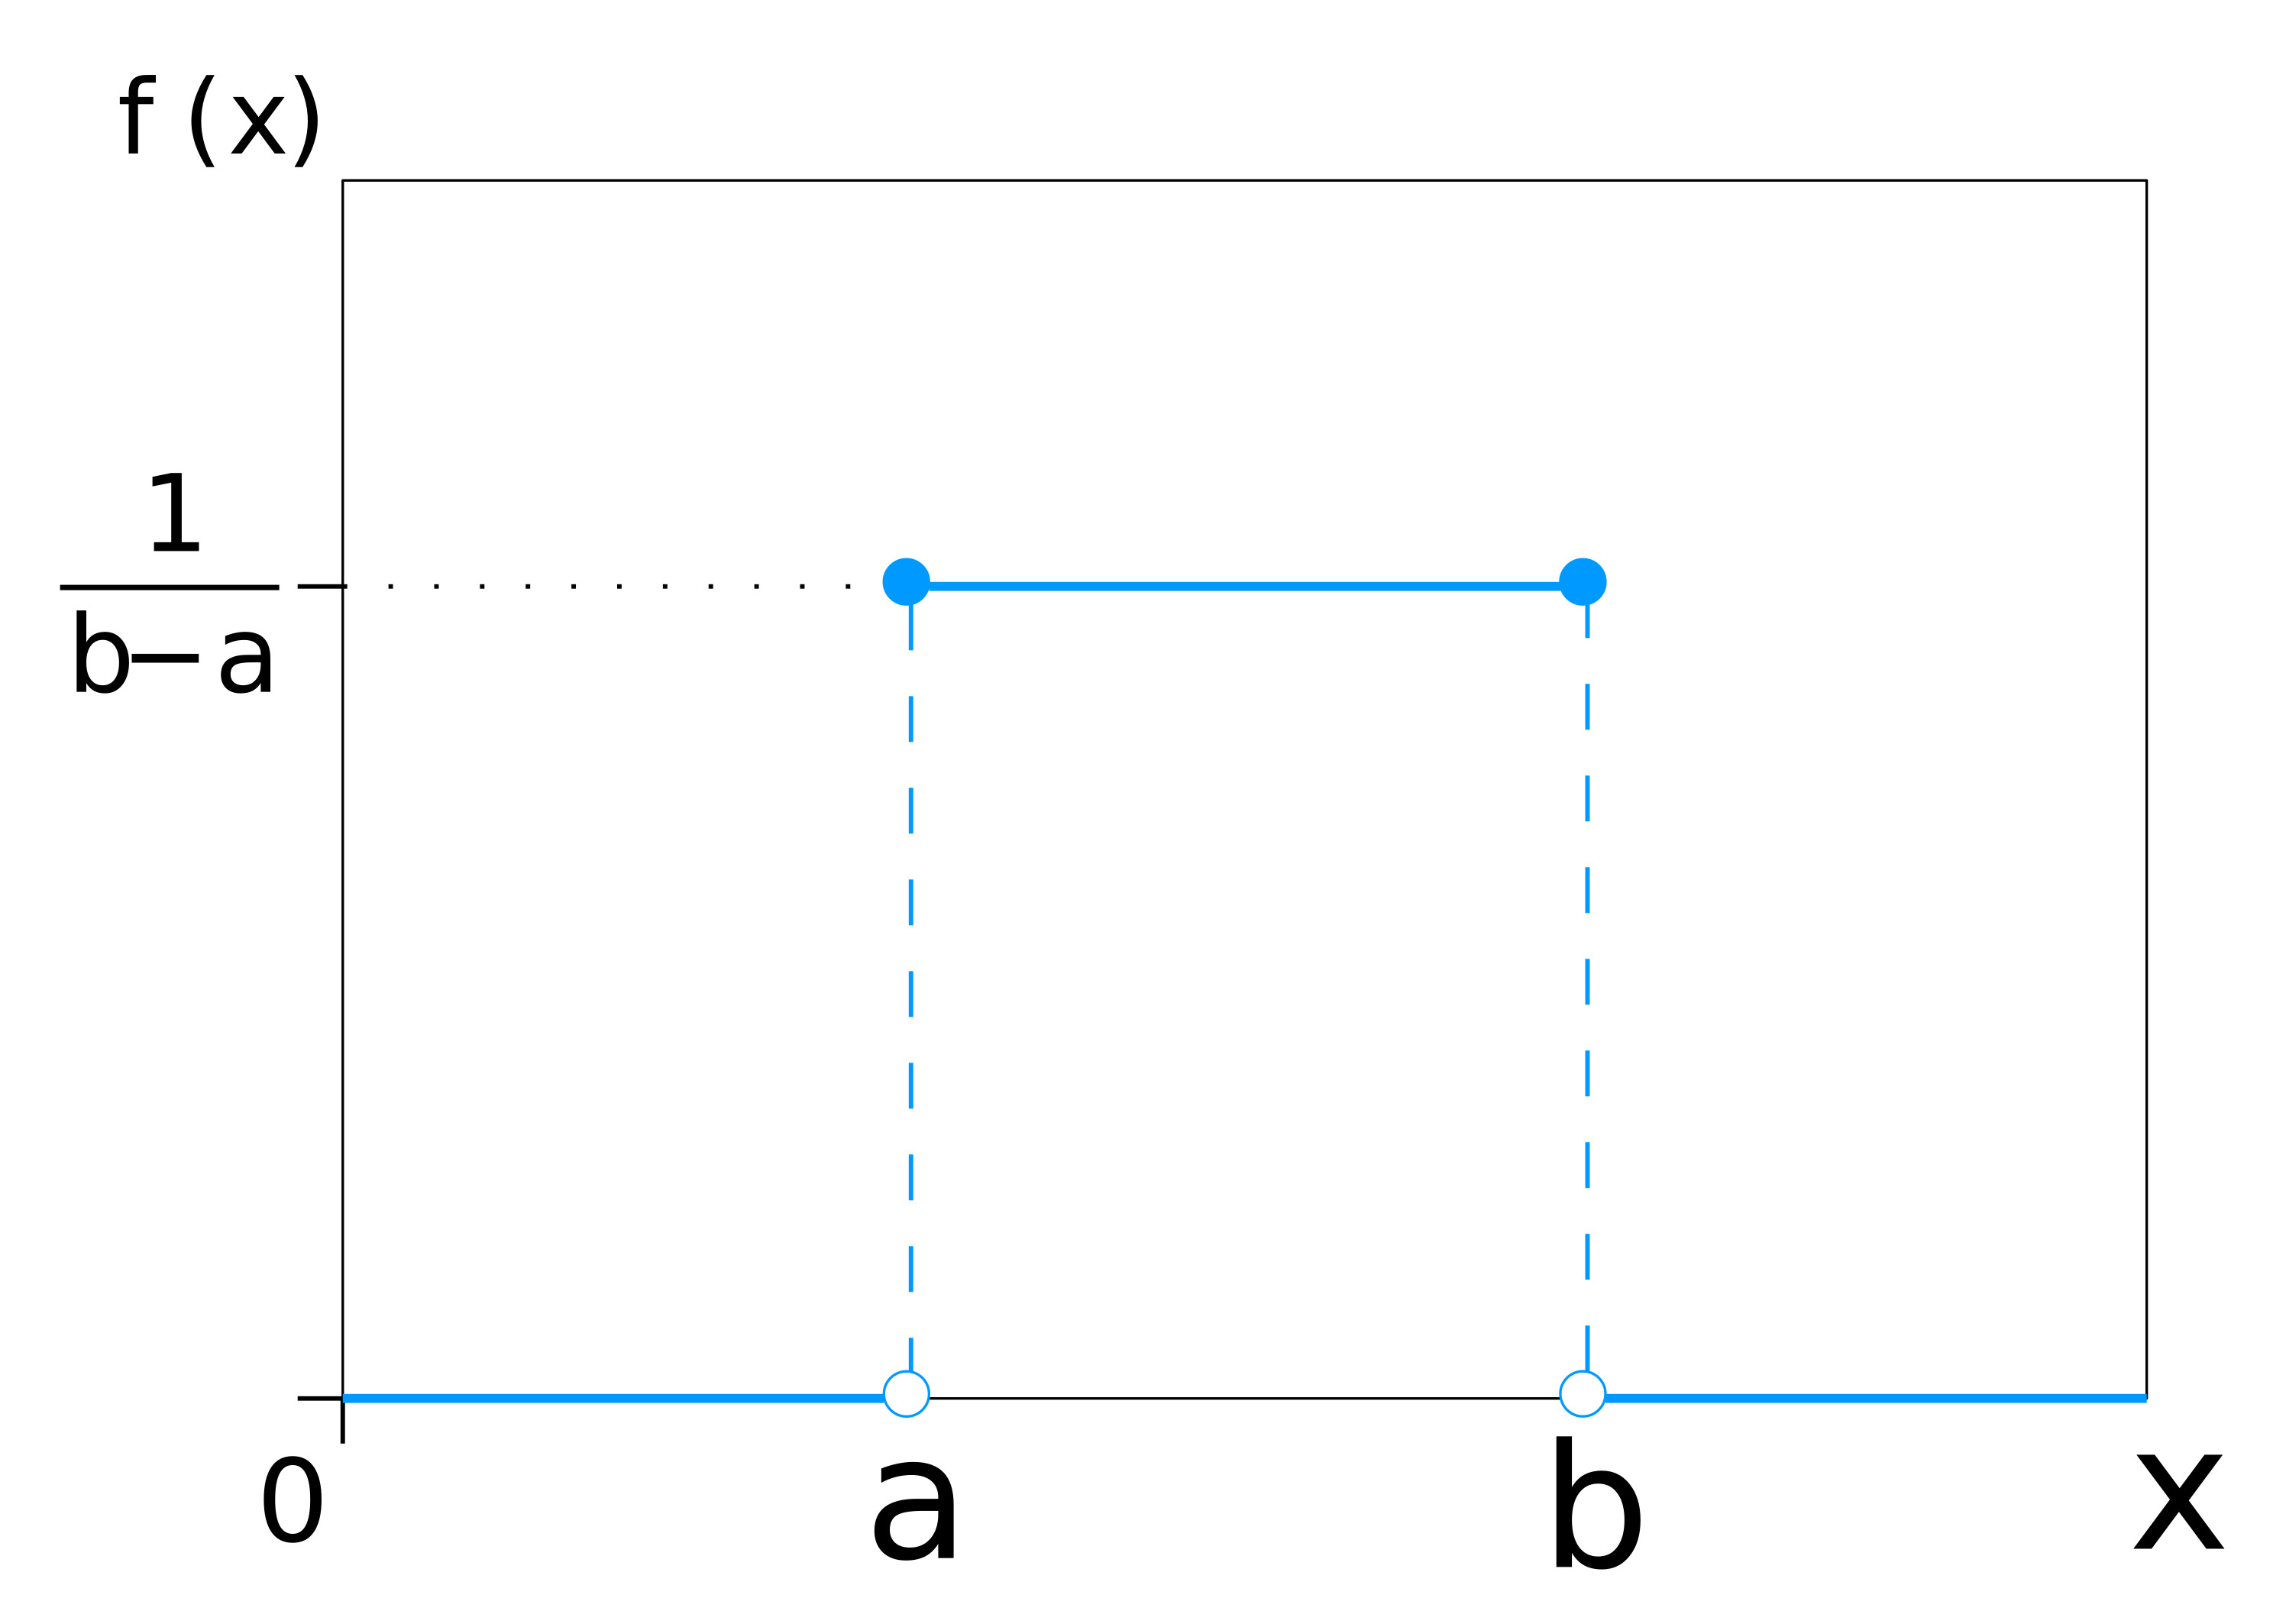
\includegraphics[width=\linewidth, height=4cm, keepaspectratio]{Pictures/distributions/Uniform_Distribution_PDF.jpg}
            \caption{(Continuous) Uniform Distribution: PDF}
        \end{figure}
    \end{minipage}
    \hfill
    \begin{minipage}{0.49\linewidth}
        \begin{figure}[H]
            \centering
            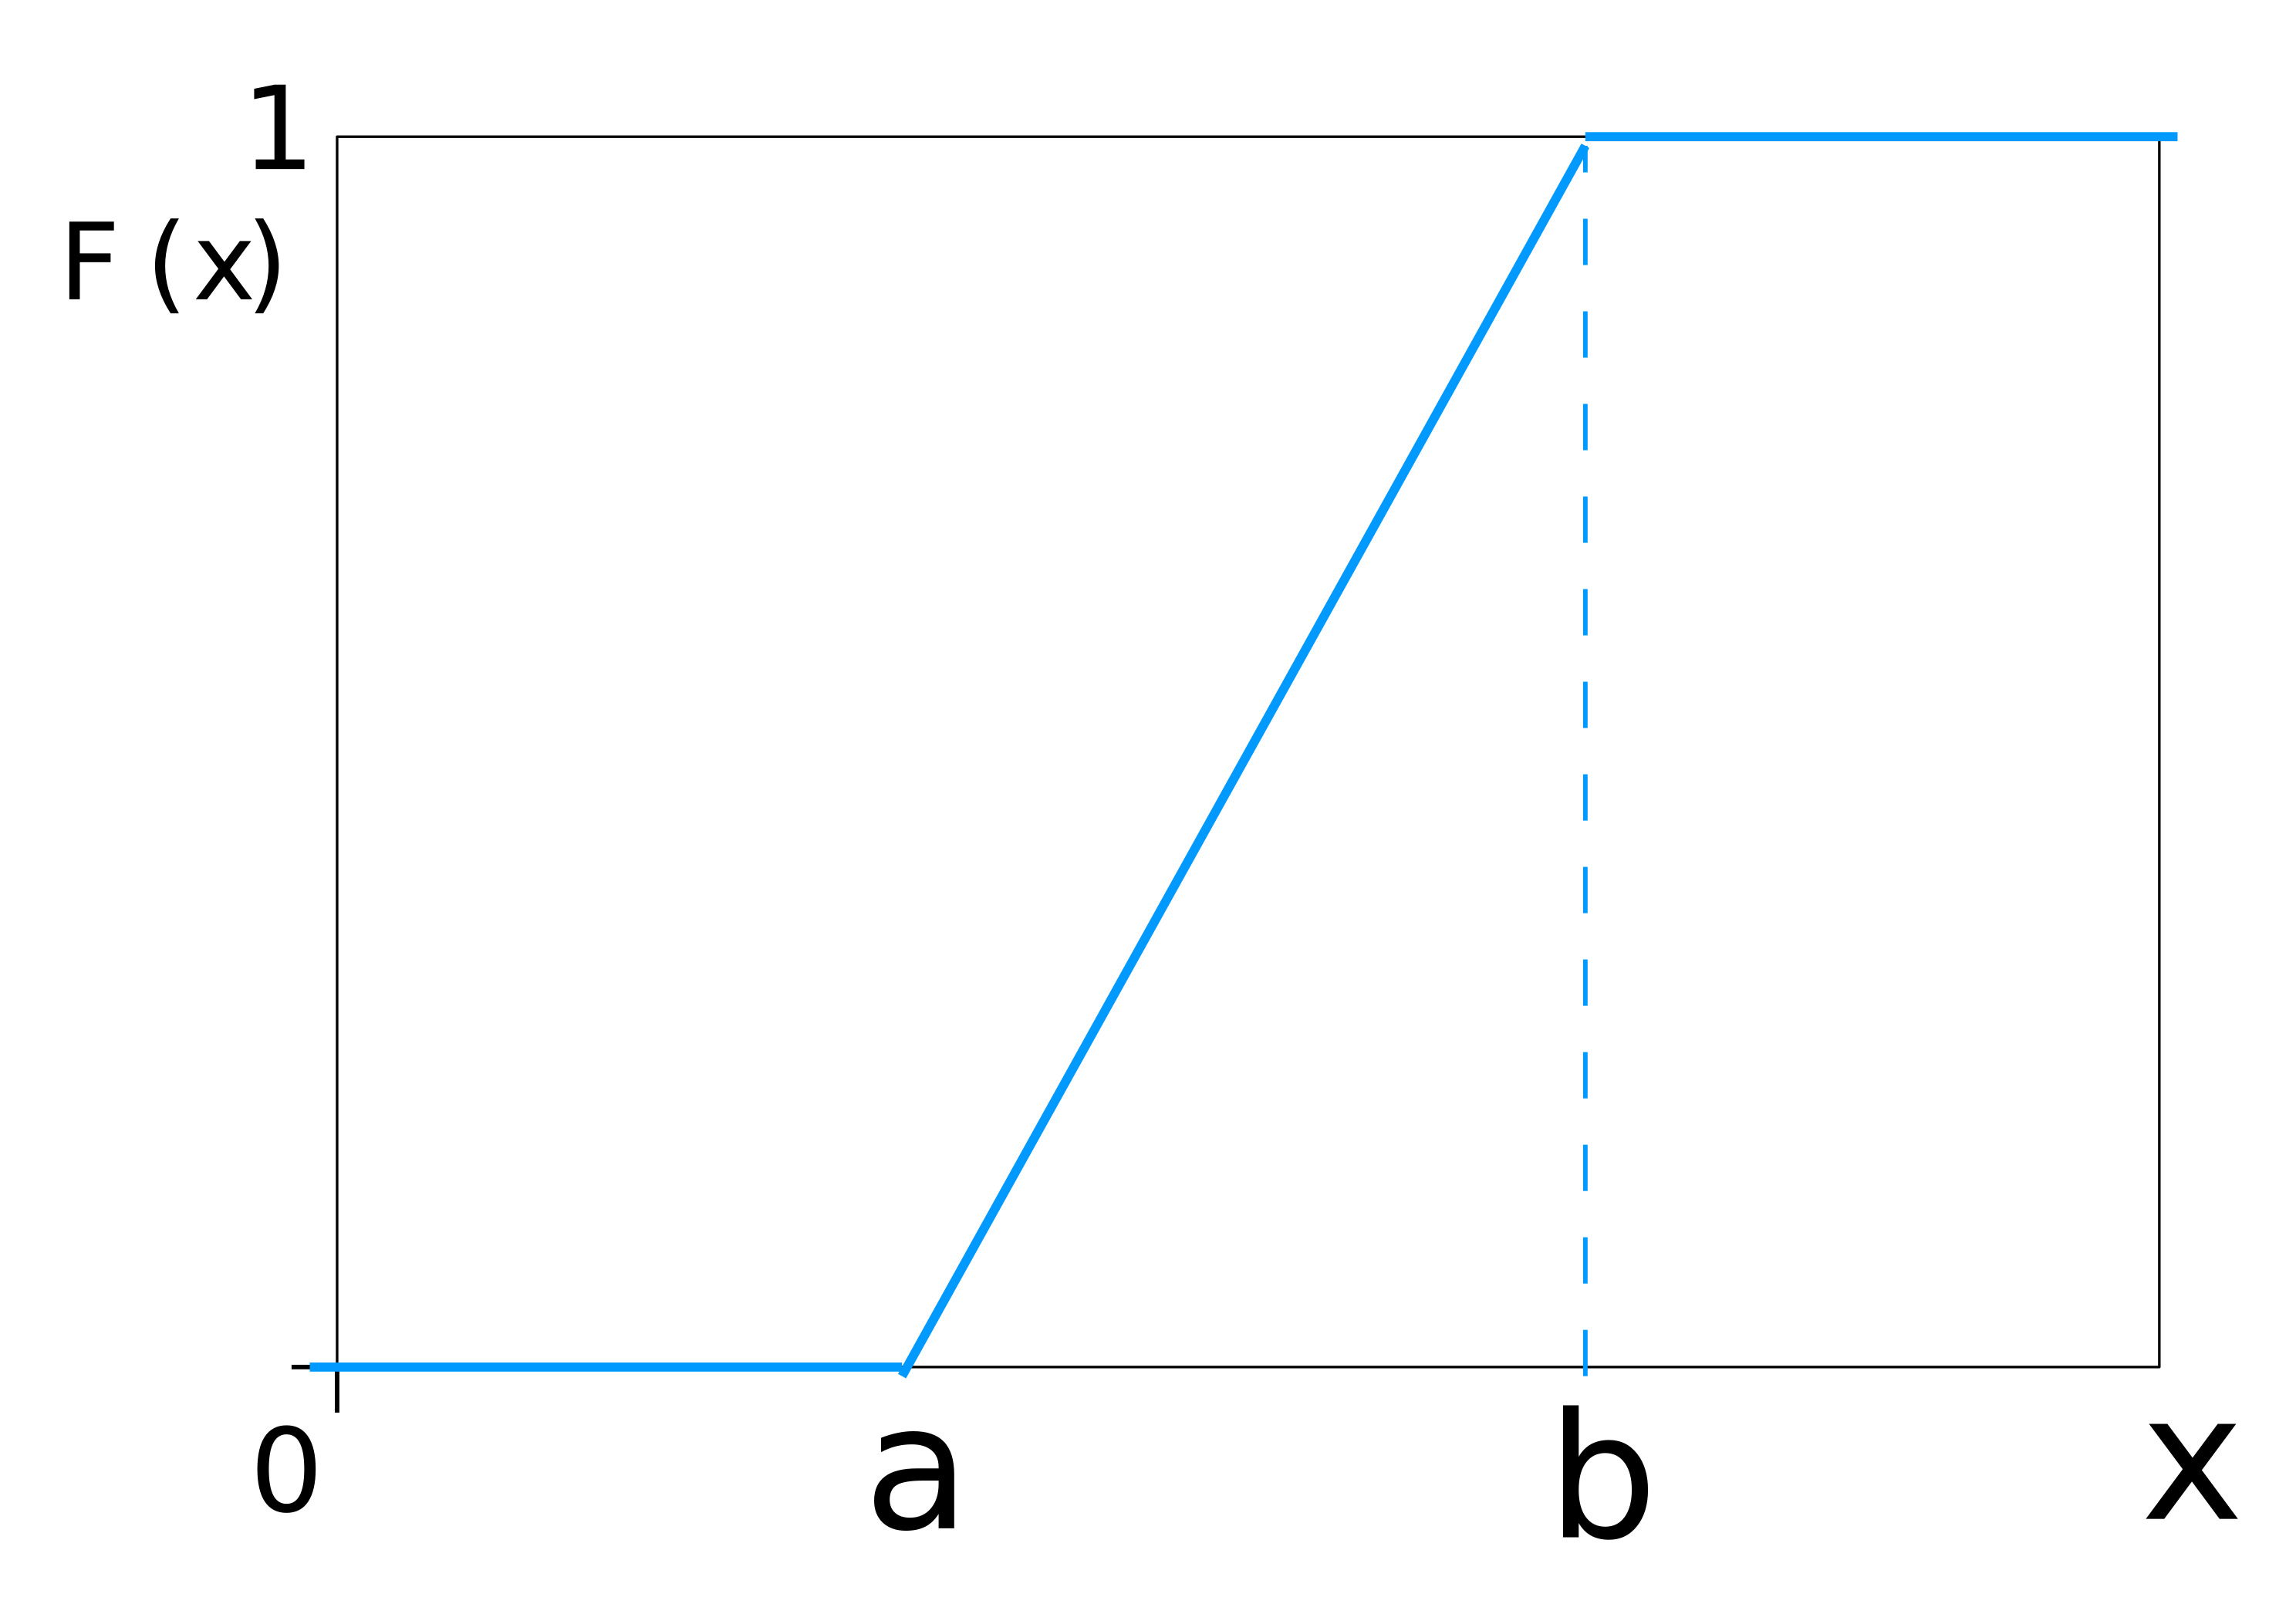
\includegraphics[width=\linewidth, height=4cm, keepaspectratio]{Pictures/distributions/Uniform_Distribution_CDF.jpg}
            \caption{(Continuous) Uniform Distribution: CDF}
        \end{figure}
    \end{minipage}
\end{table}

$a = \theta_0$ \& $b = \theta_1$

\renewcommand{\arraystretch}{2}
\begin{longtable}{|m{6cm}|p{9cm}|}
    \hline
    \multicolumn{2}{|c|}{\textbf{(Continuous) Uniform Distribution - Info} \cite{wiki/Continuous_uniform_distribution}} \\
    \hline\endfirsthead

    \hline
    \multicolumn{2}{|c|}{\textbf{(Continuous) Uniform Distribution - Info - contd.} \cite{wiki/Continuous_uniform_distribution}} \\
    \hline\endhead
    
    \hline\endfoot
    \hline\endlastfoot

    \hline
    \textbf{Notation} & 
    ${\displaystyle {\mathcal {U}}_{[\theta_0,\theta_1]}}$
    \\ \hline

    \textbf{Statistical parameters} & 
    ${\displaystyle -\infty <\theta_0<\theta_1<\infty }$
    \\ \hline
    
    \textbf{Support} & 
    ${\displaystyle [\theta_0,\theta_1]}$
    \\ \hline

    \textbf{Probability Density Function (PDF)} & 
    ${\displaystyle {\begin{cases}{\dfrac {1}{\theta_1-\theta_0}}&{\text{for }}x\in [\theta_0,\theta_1]\\0&{\text{otherwise}}\end{cases}}}$
    \\[2ex] \hline
    
    \textbf{Cumulative distribution function (CDF)} & 
    ${\displaystyle {\begin{cases}0&{\text{for }}x<\theta_0\\{\dfrac {x-\theta_0}{\theta_1-\theta_0}}&{\text{for }}x\in [\theta_0,\theta_1]\\1&{\text{for }}x>\theta_1\end{cases}}}$
    \\ \hline

    \textbf{Mean} & 
    ${\displaystyle {\dfrac {1}{2}}(\theta_0+\theta_1)}$
    \\[1ex] \hline

    \textbf{Median} & 
    ${\displaystyle {\dfrac {1}{2}}(\theta_0+\theta_1)}$
    \\[1ex] \hline

    \textbf{Mode} & 
    ${\displaystyle {\text{any value in }}(\theta_0,\theta_1)}$
    \\ \hline

    \textbf{Variance} &
    ${\displaystyle {\dfrac {1}{12}}(\theta_1-\theta_0)^{2}}$
    \\[1ex] \hline

    \textbf{Mean absolute deviation (MAD)} &
    ${\displaystyle {\dfrac {1}{4}}(\theta_1-\theta_0)}$
    \\[1ex] \hline

    \textbf{Skewness} &
    $0$
    \\ \hline

    \textbf{Excess kurtosis} &
    ${\displaystyle -{\dfrac {6}{5}}}$
    \\[1ex] \hline

    \textbf{Entropy} &
    ${\displaystyle \log(\theta_1-\theta_0)}$
    \\[1ex] \hline

    \textbf{Moment-generating function (MGF)} &
    ${\displaystyle {\begin{cases}{\dfrac {\mathrm {e} ^{t\theta_1}-\mathrm {e} ^{t\theta_0}}{t(\theta_1-\theta_0)}}&{\text{for }}t\neq 0\\1&{\text{for }}t=0\end{cases}}}$
    \\[1ex] \hline

    \textbf{Characteristic function (CF)} &
    ${\displaystyle {\begin{cases}{\dfrac {\mathrm {e} ^{\mathrm {i} t\theta_1}-\mathrm {e} ^{\mathrm {i} t\theta_0}}{\mathrm {i} t(\theta_1-\theta_0)}}&{\text{for }}t\neq 0\\1&{\text{for }}t=0\end{cases}}}$
    \\[1ex] \hline

\end{longtable}
\renewcommand{\arraystretch}{1}

Parameters:
\begin{enumerate}
    \item $\theta_0$ : minimum value of population, $\theta_1$ : maximum value of population

    \item 
        \hfill
        $\theta_0 < \theta_1$
        \hfill
        $\theta_0 \leq x \leq \theta_1$
        \hfill

\end{enumerate}



\section{(Continuous) Standard Uniform Distribution ($X \sim \mathcal{U}(0,1)$) \cite{ism-1}} \label{Standard Uniform Distribution}

\begin{enumerate}
    \item $\theta_0 = 0$ and $\theta_1 = 1$

\end{enumerate}



























\chapter{Exponential Distribution ($X \sim \exp(\lambda)$) \cite{ism-1,wiki/Exponential_distribution}} \label{Exponential Distribution}

\begin{table}[H]
    \begin{minipage}{0.49\linewidth}
        \begin{figure}[H]
            \centering
            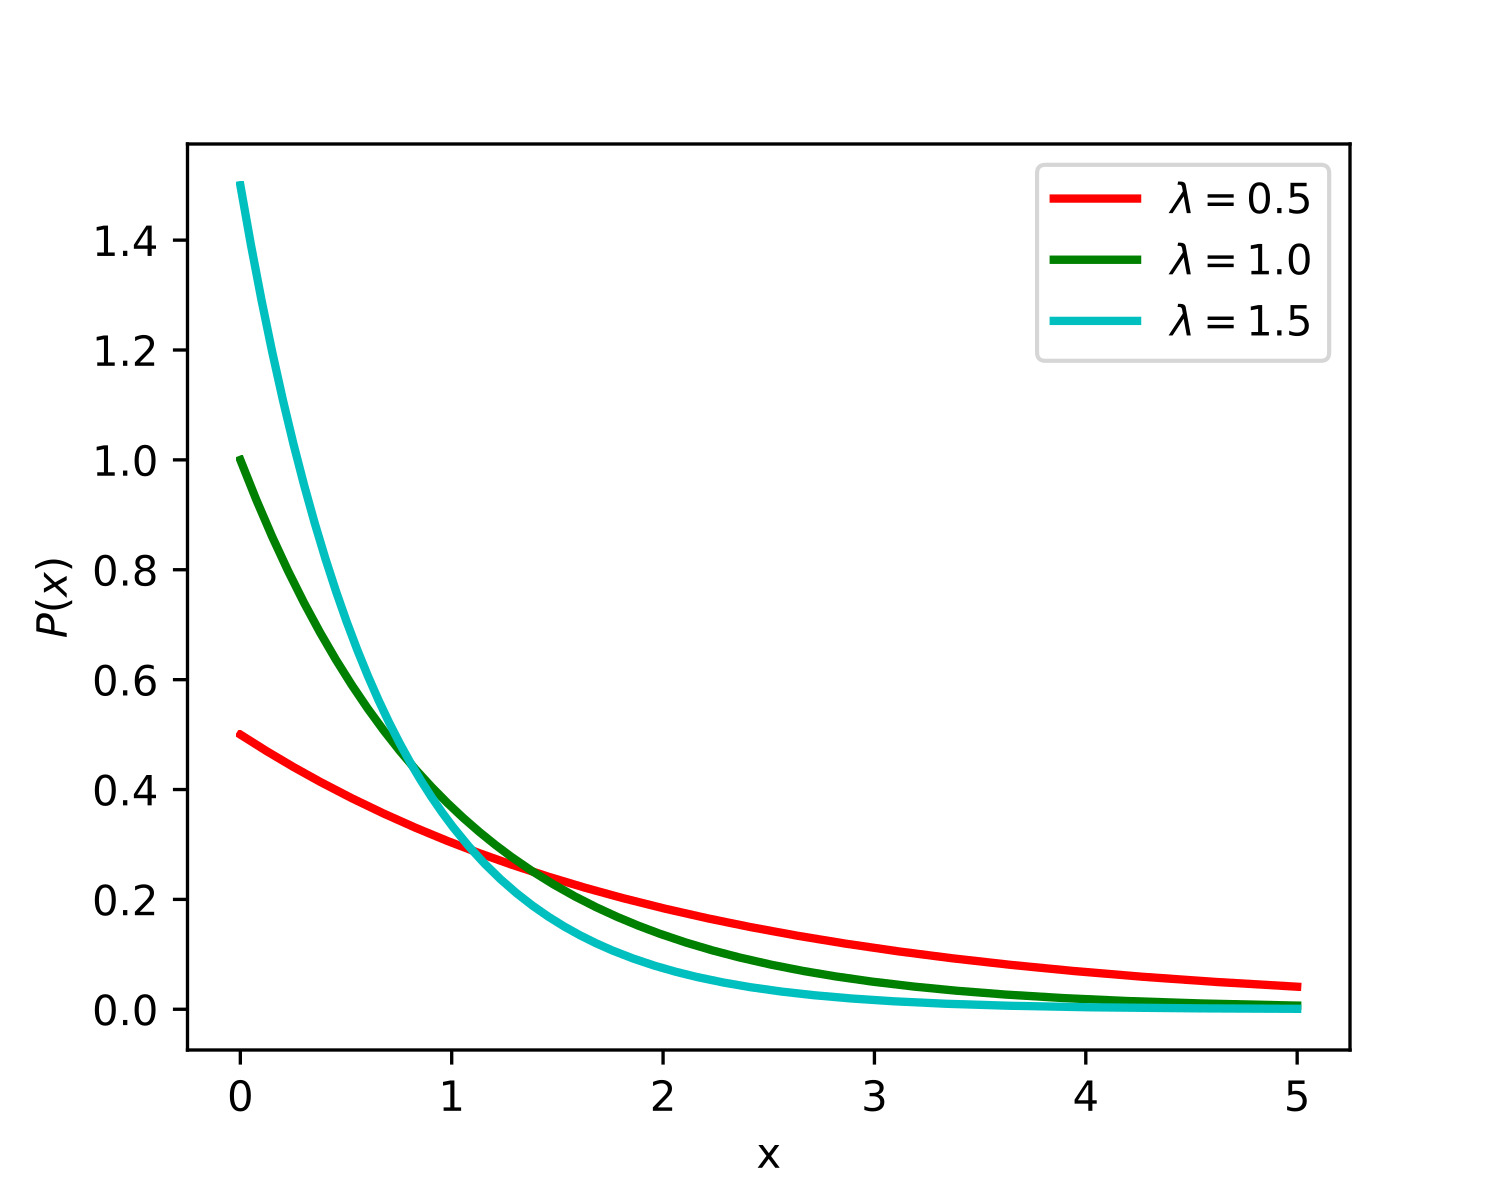
\includegraphics[width=\linewidth, height=4cm, keepaspectratio]{Pictures/distributions/Exponential_distribution_pdf.jpg}
            \caption{Exponential Distribution: PDF}
        \end{figure}
    \end{minipage}
    \hfill
    \begin{minipage}{0.49\linewidth}
        \begin{figure}[H]
            \centering
            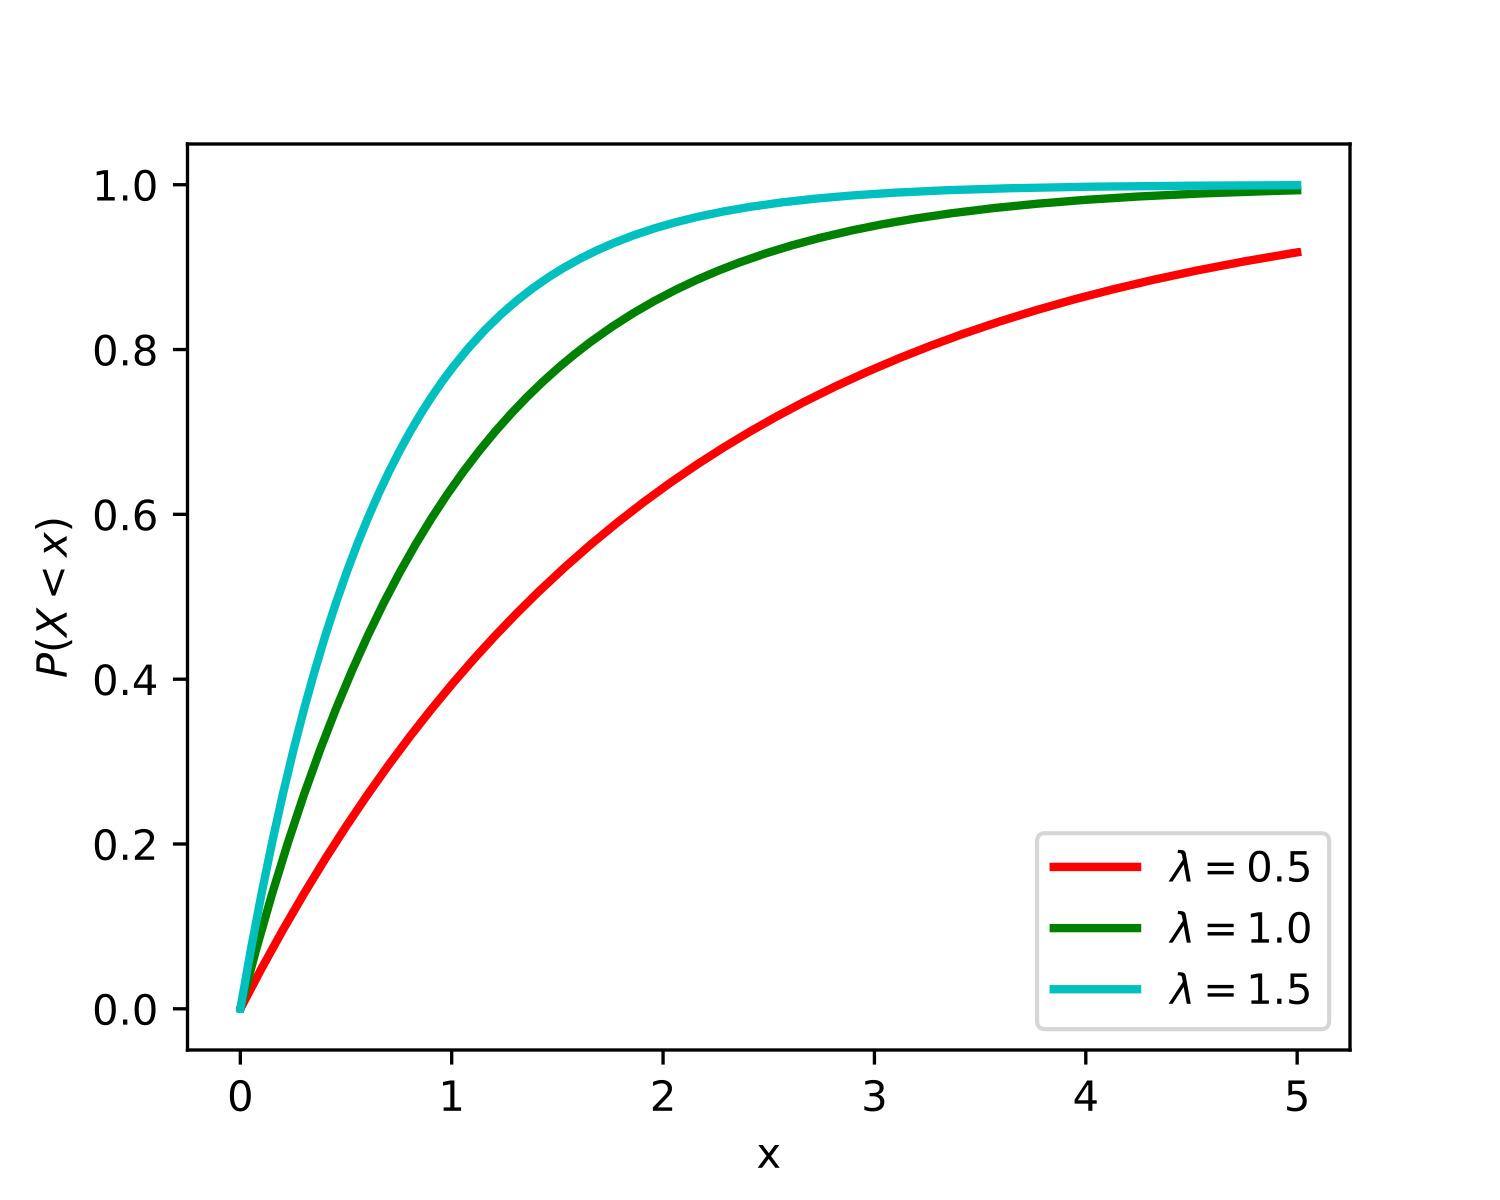
\includegraphics[width=\linewidth, height=4cm, keepaspectratio]{Pictures/distributions/Exponential_distribution_cdf.jpg}
            \caption{Exponential Distribution: CDF}
        \end{figure}
    \end{minipage}
\end{table}

\begin{customTableWrapper}{2}
\begin{longtable}{|m{6cm}|p{9cm}|}
    \hline
    \customTableHeaderColor
    \multicolumn{2}{|c|}{\textbf{Exponential Distribution - Info} \cite{wiki/Exponential_distribution}} \\
    \hline\endfirsthead

    \hline
    \customTableHeaderColor
    \multicolumn{2}{|c|}{\textbf{Exponential Distribution - Info - contd.} \cite{wiki/Exponential_distribution}} \\
    \hline\endhead
    
    \hline\endfoot
    \hline\endlastfoot

    \textbf{Statistical parameters} & 
    ${ \lambda >0}$ rate, or inverse scale
    \\ \hline
    
    \textbf{Support} &
    ${ x\in [0,\infty )}$
    \\ \hline

    \textbf{Probability Density Function (PDF)} & 
    ${ \lambda e^{-\lambda x}}$
    \\[1ex] \hline
    
    \textbf{Cumulative distribution function (CDF)} & 
    ${ 1-e^{-\lambda x}}$
    \\ \hline

    \textbf{Quantile} &
    ${ -{\dfrac {\ln(1-p)}{\lambda }}}$
    \\ \hline

    \textbf{Mean} & 
    ${ {\dfrac {1}{\lambda }}}$
    \\[1ex] \hline

    \textbf{Median} & 
    ${ {\dfrac {\ln (2)}{\lambda }}}$
    \\[1ex] \hline

    \textbf{Mode} & 
    $0$
    \\ \hline

    \textbf{Variance} &
    ${ {\dfrac {1}{\lambda ^{2}}}}$
    \\[1ex] \hline

    \textbf{Skewness} &
    $2$
    \\ \hline

    \textbf{Excess kurtosis} &
    $6$
    \\ \hline

    \textbf{Entropy} &
    ${ 1-\ln (\lambda) }$
    \\[1ex] \hline

    \textbf{Moment-generating function (MGF)} &
    ${ {\dfrac {\lambda }{\lambda -t}},{\text{ for }}t<\lambda }$
    \\[1ex] \hline

    \textbf{Characteristic function (CF)} &
    ${ {\dfrac {\lambda }{\lambda -it}}}$
    \\[1ex] \hline

    \textbf{Fisher information} &
    ${ {\frac {1}{\lambda ^{2}}}}$
    \\[1ex] \hline

    \textbf{Kullback–Leibler divergence} &
    ${ \ln {\dfrac {\lambda _{0}}{\lambda }}+{\dfrac {\lambda }{\lambda _{0}}}-1}$
    \\[1ex] \hline

    \textbf{Expected shortfall} &
    ${ {\dfrac {-\ln(1-p)+1}{\lambda }}}$
    \\[1ex] \hline

    \textbf{Inverse of CDF \cite{ism-1}} &
    $F_\lambda^{-1}(u) = -\dfrac{\log(1-u)}{\lambda}$ $u \in (0,1)$
    \\[1ex] \hline

    \textbf{Relative Standard Deviation} &
    $1$
    \\[1ex] \hline

\end{longtable}
\end{customTableWrapper}


\section{Sample Statistic Minimum ($X_{(1)}$) \cite{ism-1}} \label{Exponential Distribution: Sample Statistic Minimum}

\begin{enumerate}
    \item $F_{X_{(1)}}(x) = 1 - \exp(-n\lambda x)$

    \item The sample distribution of the minimum X(1) is exponentially distributed, 
    \[
        X_{(1)} \sim \exp(n\lambda)
    \]
    but now with parameter $n\lambda$, when $X_1,X_2,\cdots, X_n$ are i.i.d. $exp(\lambda)$ distributed.
    
\end{enumerate}


\section{Using Farlie–Gumbel–Morgenstern (FGM) \cite{ism-1}} \label{Sample Statistic Minimum: Using Farlie–Gumbel–Morgenstern (FGM)}

\begin{enumerate}[itemsep=0.2cm]
    \item $
            \hfill
            F_X : \lambda_X
            \hfill
            F_Y : \lambda_Y
            \hfill
        $

    \item $
            \hfill
            E[X(1 - 2F_X(X))] = -[2\lambda_X]^{-1}
            \hfill
            E[Y(1 - 2F_Y(Y))] = -[2\lambda_Y]^{-1}
            \hfill
        $

    \item covariance   : $-\dfrac{\alpha}{[4\lambda_X\lambda_Y]}$

    \item Pearson’s correlation : $\rho_P = -\dfrac{\alpha}{4}$

    \item product-moment correlation:
    \begin{enumerate}[itemsep=0.2cm]
        \item $\alpha$ can be estimated by $r_P\bar{X}\bar{Y}$

        \item $r_P$ estimates $\alpha\lambda _X^{-1}\lambda_Y^{-1}$

        \item $\bar{X}$ estimates the parameter $\lambda_X^{-1}$

        \item $\bar{Y}$ estimates the parameter $\lambda_Y^{-1}$
    \end{enumerate}

\end{enumerate}


\section{Double Exponential Distribution \cite{ism-1}} \label{Double Exponential Distribution}

\begin{customTableWrapper}{2}
\begin{longtable}{|m{6cm}|p{9cm}|}
    \hline
    \customTableHeaderColor
    \multicolumn{2}{|c|}{\textbf{Double Exponential Distribution - Info}} \\
    \hline\endfirsthead

    \hline
    \customTableHeaderColor
    \multicolumn{2}{|c|}{\textbf{Double Exponential Distribution - Info - contd.}} \\
    \hline\endhead
    
    \hline\endfoot
    \hline\endlastfoot

    \textbf{Statistical parameters} & 
    ${ \lambda >0}$ rate, or inverse scale
    \\ \hline
    
    \textbf{Support} &
    ${ x\in [0,\infty )}$
    \\ \hline

    \textbf{Probability Density Function (PDF)} & 
    $0.5f_\lambda(\dabs{x})$
    \\[1ex] \hline
    
    \textbf{Mean} & 
    $0$
    \\[1ex] \hline

    \textbf{Variance} &
    $\dfrac{2}{\lambda}$
    \\[1ex] \hline

    \textbf{Skewness} &
    $0$
    \\ \hline

    \textbf{Excess kurtosis} &
    $3$
    \\ \hline

\end{longtable}
\end{customTableWrapper}























\chapter{Chi-square Distribution ($X \sim \chi^2_k$) \cite{ism-1,wiki/Chi-squared_distribution}} \label{Chi-square Distribution}

\begin{table}[H]
    \begin{minipage}{0.49\linewidth}
        \begin{figure}[H]
            \centering
            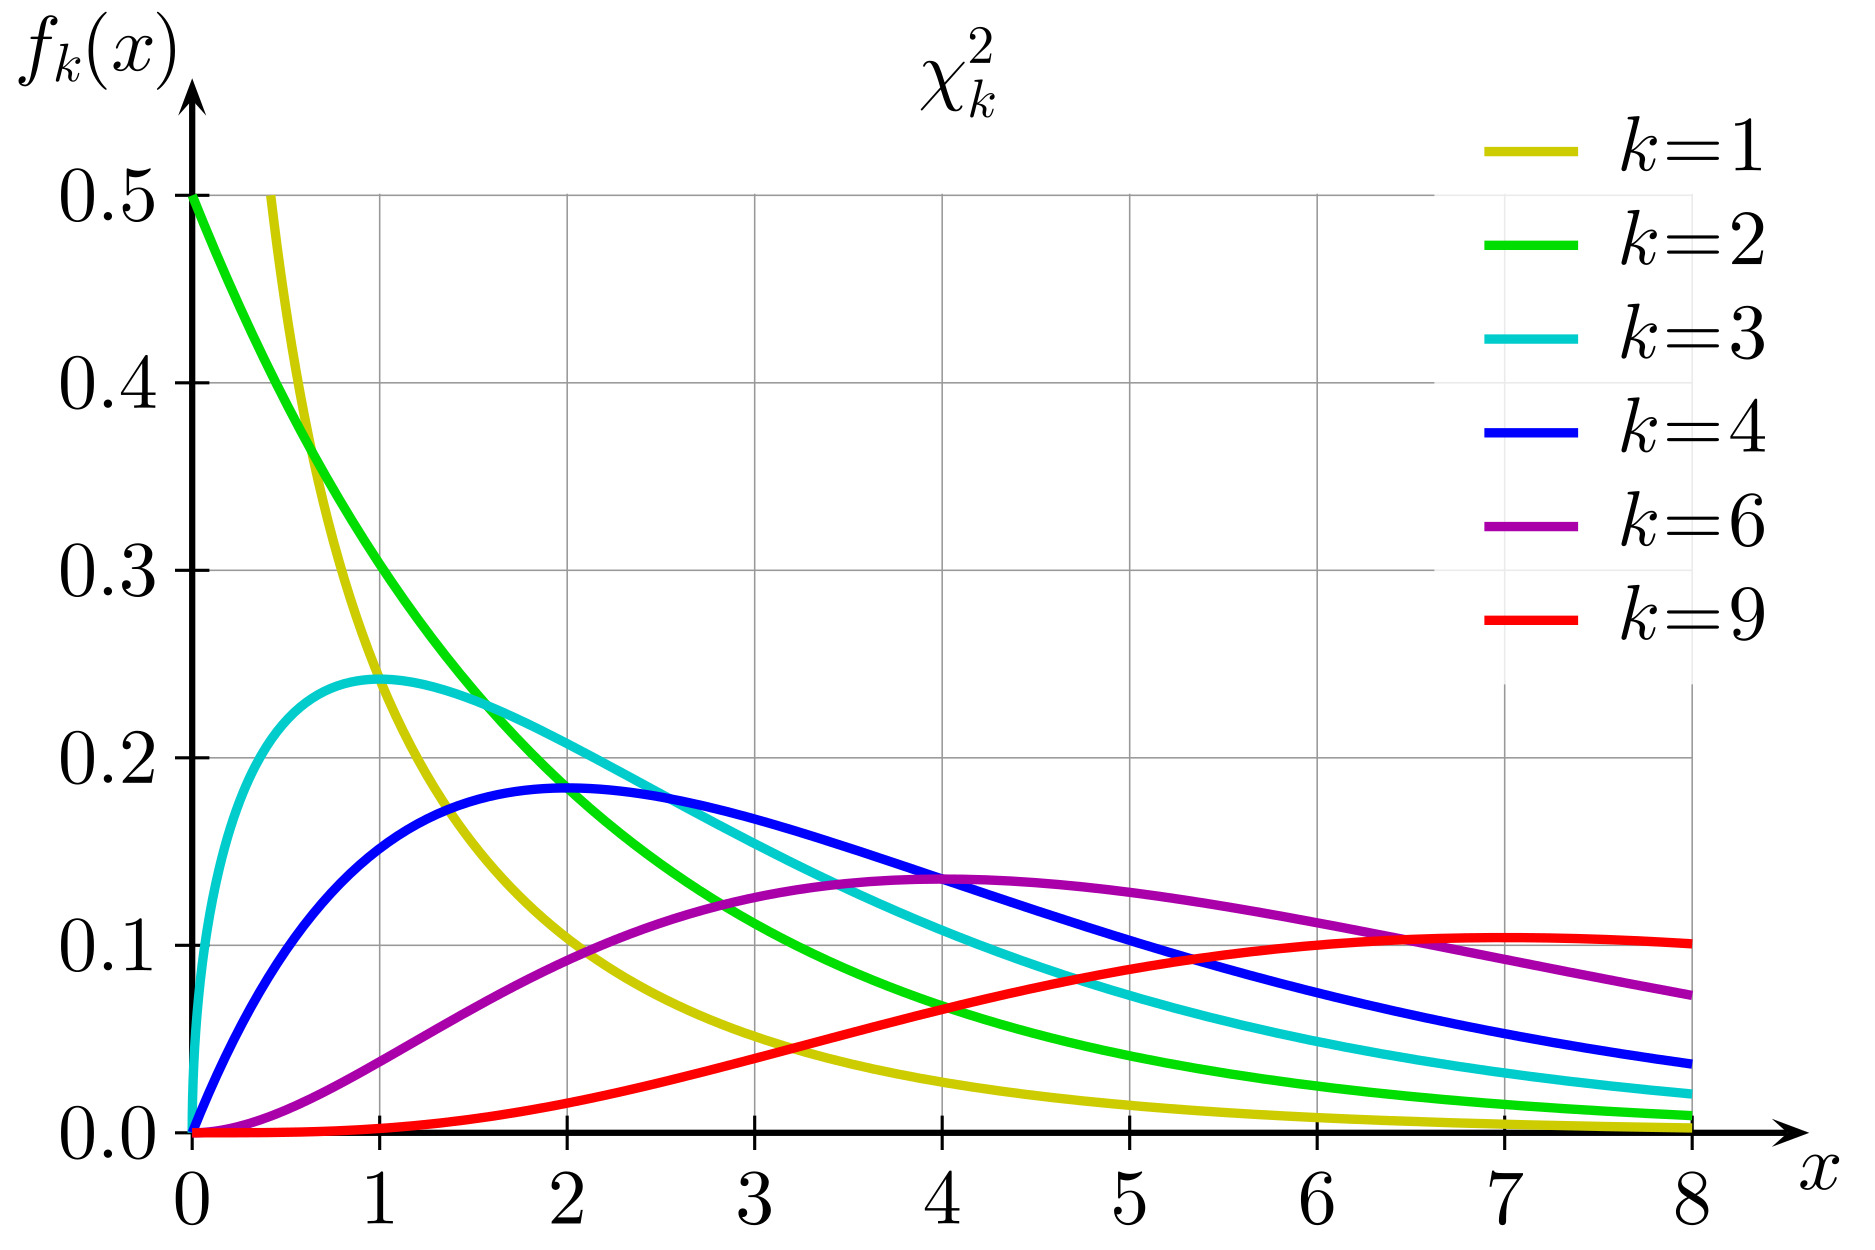
\includegraphics[width=\linewidth, height=4cm, keepaspectratio]{Pictures/distributions/Chi-square_pdf.jpg}
            \caption{Chi-square Distribution: PDF}
        \end{figure}
    \end{minipage}
    \hfill
    \begin{minipage}{0.49\linewidth}
        \begin{figure}[H]
            \centering
            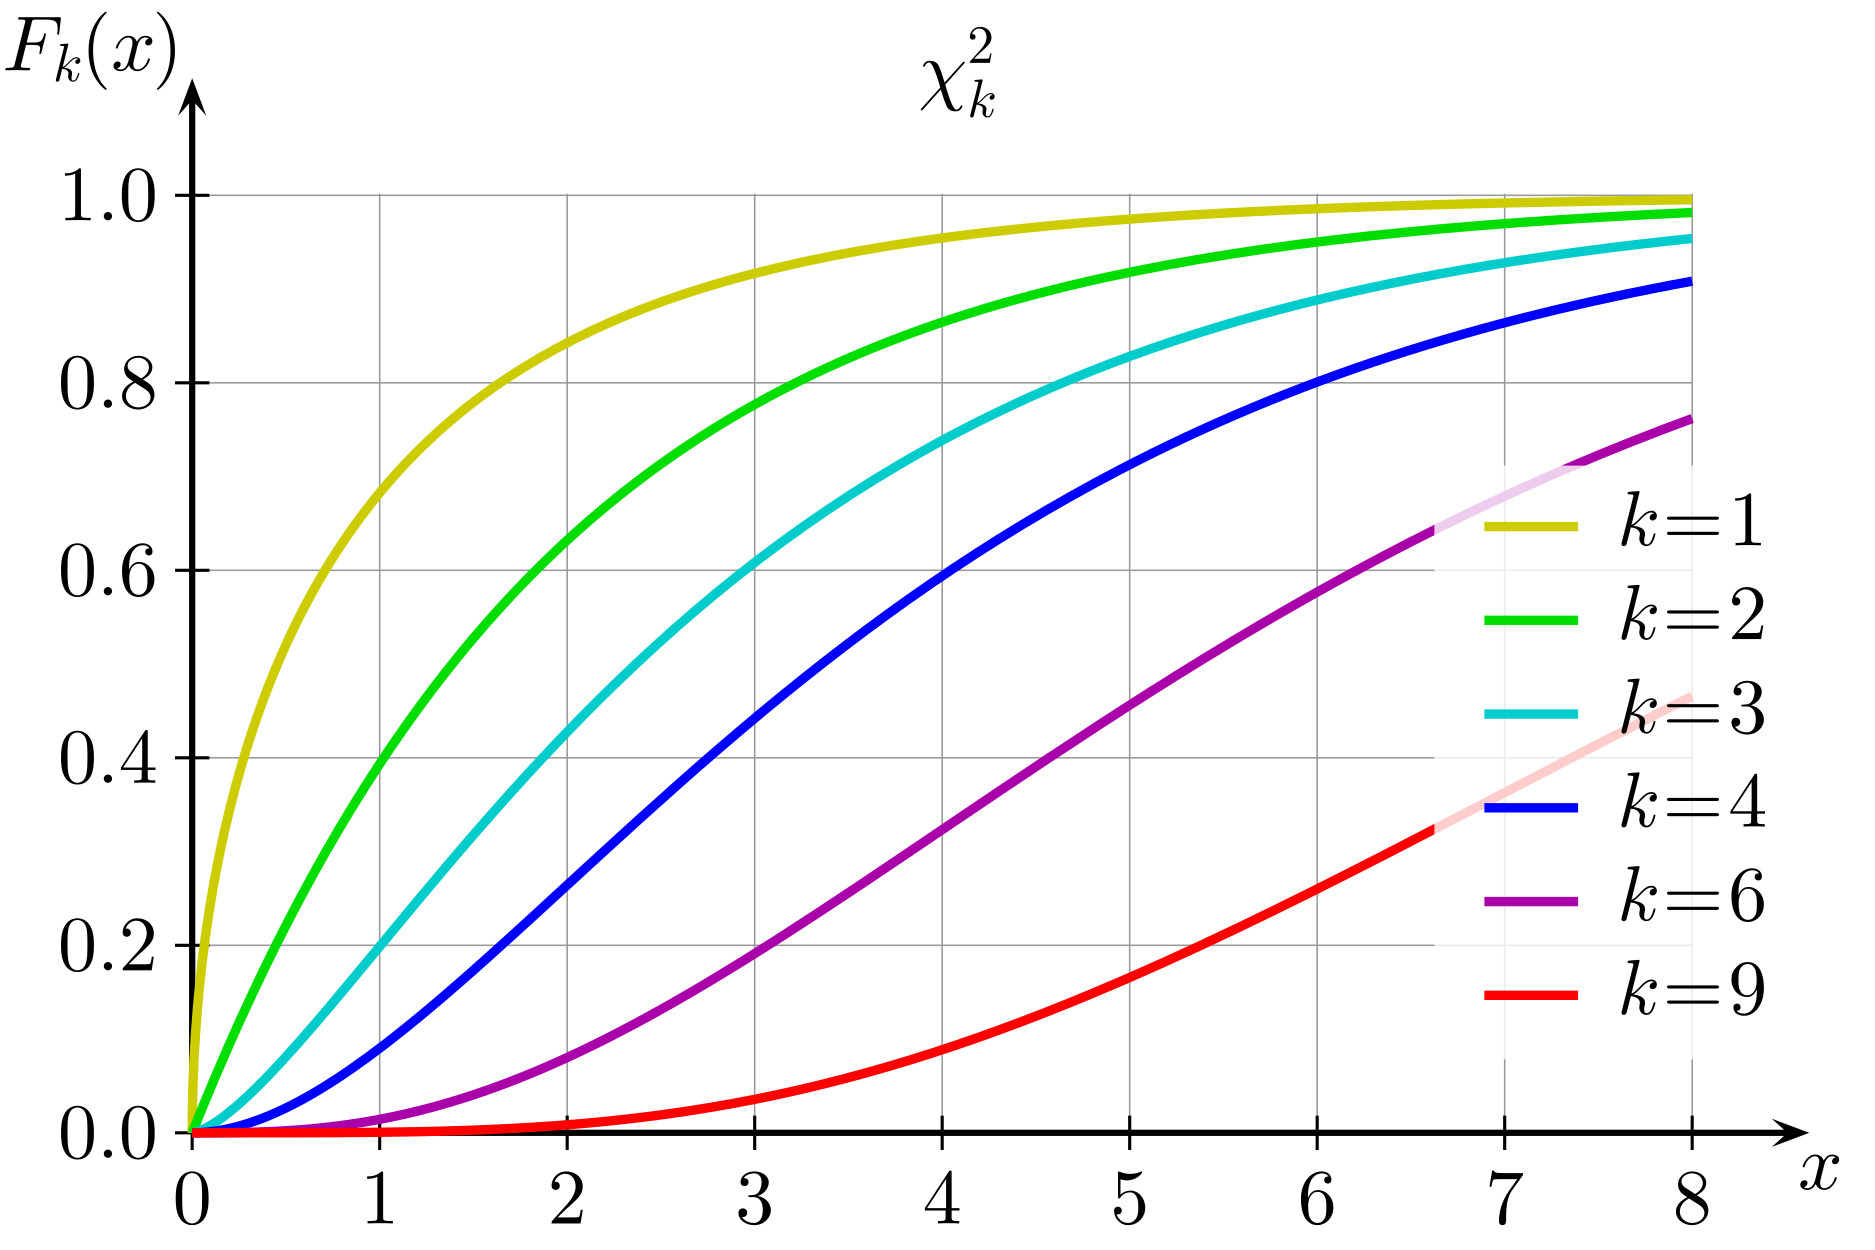
\includegraphics[width=\linewidth, height=4cm, keepaspectratio]{Pictures/distributions/Chi-square_cdf.jpg}
            \caption{Chi-square Distribution: CDF}
        \end{figure}
    \end{minipage}
\end{table}

\renewcommand{\arraystretch}{2}
\begin{longtable}{|m{6cm}|p{9cm}|}
    \hline
    \multicolumn{2}{|c|}{\textbf{Chi-square Distribution - Info} \cite{wiki/Chi-squared_distribution}} \\
    \hline\endfirsthead

    \hline
    \multicolumn{2}{|c|}{\textbf{Chi-square Distribution - Info - contd.} \cite{wiki/Chi-squared_distribution}} \\
    \hline\endhead
    
    \hline\endfoot
    \hline\endlastfoot

    \textbf{Notation} &
    ${\displaystyle \chi ^{2}(k)\;}$ or ${\displaystyle \chi _{k}^{2}\!}$
    \\ \hline

    \textbf{Statistical parameters} & 
    ${\displaystyle k\in \mathbb {N} ^{*}~~}$ (known as "degrees of freedom")
    \\ \hline
    
    \textbf{Support} &
    ${\displaystyle x\in [0,+\infty )\;}$
    \\ \hline

    \textbf{Probability Density Function (PDF)} & 
    ${\displaystyle {\dfrac {1}{2^{k/2}\Gamma (k/2)}}\;x^{k/2-1}e^{-x/2}\;}$
    \\[1ex] \hline
    
    \textbf{Cumulative distribution function (CDF)} & 
    ${\displaystyle {\dfrac {1}{\Gamma (k/2)}}\;\gamma \left({\dfrac {k}{2}},\,{\dfrac {x}{2}}\right)\;}$
    \\ \hline

    \textbf{Mean} & 
    $k$
    \\[1ex] \hline

    \textbf{Median} & 
    ${\displaystyle \approx k{\bigg (}1-{\dfrac {2}{9k}}{\bigg )}^{3}\;}$
    \\[1ex] \hline

    \textbf{Mode} & 
    ${\displaystyle \max(k-2,0)\;}$
    \\ \hline

    \textbf{Variance} &
    $2k$
    \\[1ex] \hline

    \textbf{Skewness} &
    ${\displaystyle {\sqrt {\dfrac{8}{k}}}\,}$
    \\[1ex] \hline

    \textbf{Excess kurtosis} &
    ${\displaystyle {\dfrac {12}{k}}}$
    \\[1ex] \hline

    \textbf{Entropy} &
    ${\displaystyle {{\dfrac {k}{2}} +\log \left(2\Gamma {\Bigl (}{\dfrac {k}{2}}{\Bigr )}\right)+\left(1-{\dfrac {k}{2}}\right)\psi \left({\dfrac {k}{2}}\right)}}$
    \\[1ex] \hline

    \textbf{Moment-generating function (MGF)} &
    ${\displaystyle (1-2t)^{-k/2}{\text{ for }}t<{\frac {1}{2}}\;}$
    \\[1ex] \hline

    \textbf{Characteristic function (CF)} &
    ${\displaystyle (1-2it)^{-k/2}}$
    \\[1ex] \hline

    \textbf{Probability-generating function (PGF)} &
    ${\displaystyle (1-2\ln t)^{-k/2}{\text{ for }}0<t<{\sqrt {e}}\;}$
    \\[1ex] \hline

\end{longtable}
\renewcommand{\arraystretch}{1}

\begin{enumerate}[itemsep=0.2cm]
    \item Confidence Interval:
    \begin{enumerate}[itemsep=0.2cm]
        \item $V_{n-1}^2 = (n-1)S^2/\sigma^2 \sim \chi_{n-1}^2$

        \item $p$th quantile of the chi-square distribution with $n - 1$ DOF: $x_p(f_{\chi^2})$

        \item $
            \hfill
            Pr(V_{n-1}^2 \leq x_p(f_{\chi^2})) = p
            \hfill
            Pr(V_{n-1}^2 > x_{1-p}(f_{\chi^2})) = p
            \hfill
        $

        \item $
            Pr(\sigma^2 < (n-1)S^2/x_{1-p}(f_{\chi^2})) = p 
        $

        \item $1 - 2p$ confidence interval for the variance $\sigma^2$ is:
        \[[
            (n-1)S^2/x_{1-p}(f_{\chi^2}), 
            \hspace{0.2cm}
            (n-1)S^2/x_{p}(f_{\chi^2})
        )\]

    \end{enumerate}

\end{enumerate}


































\chapter{Student's t-Distribution ($X \sim t_\nu$) \cite{ism-1,wiki/Student_t-distribution}}\label{Student's t-Distribution}

\begin{table}[H]
    \begin{minipage}{0.49\linewidth}
        \begin{figure}[H]
            \centering
            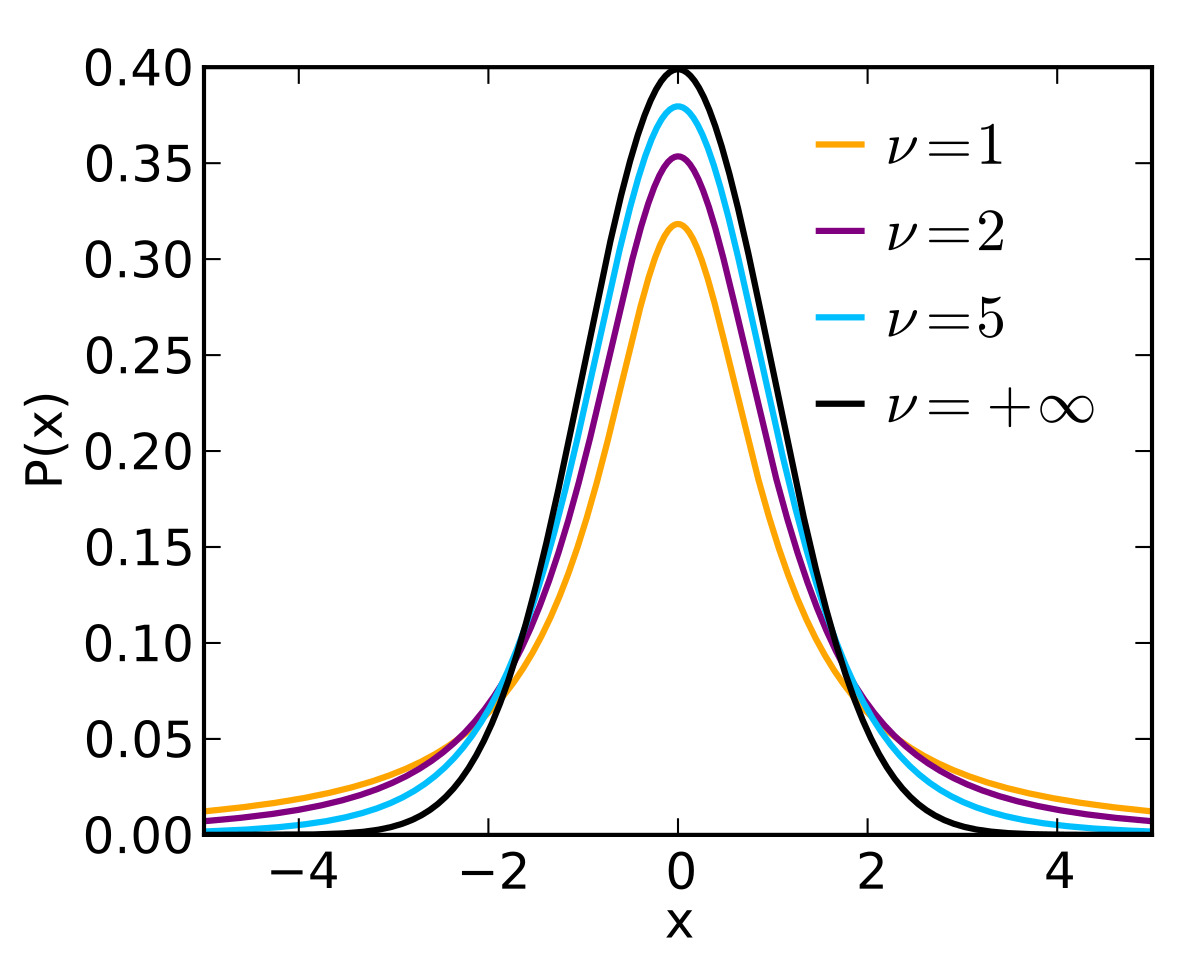
\includegraphics[width=\linewidth, height=4cm, keepaspectratio]{Pictures/distributions/Student_t_pdf.jpg}
            \caption{Student's t-Distribution: PDF}
        \end{figure}
    \end{minipage}
    \hfill
    \begin{minipage}{0.49\linewidth}
        \begin{figure}[H]
            \centering
            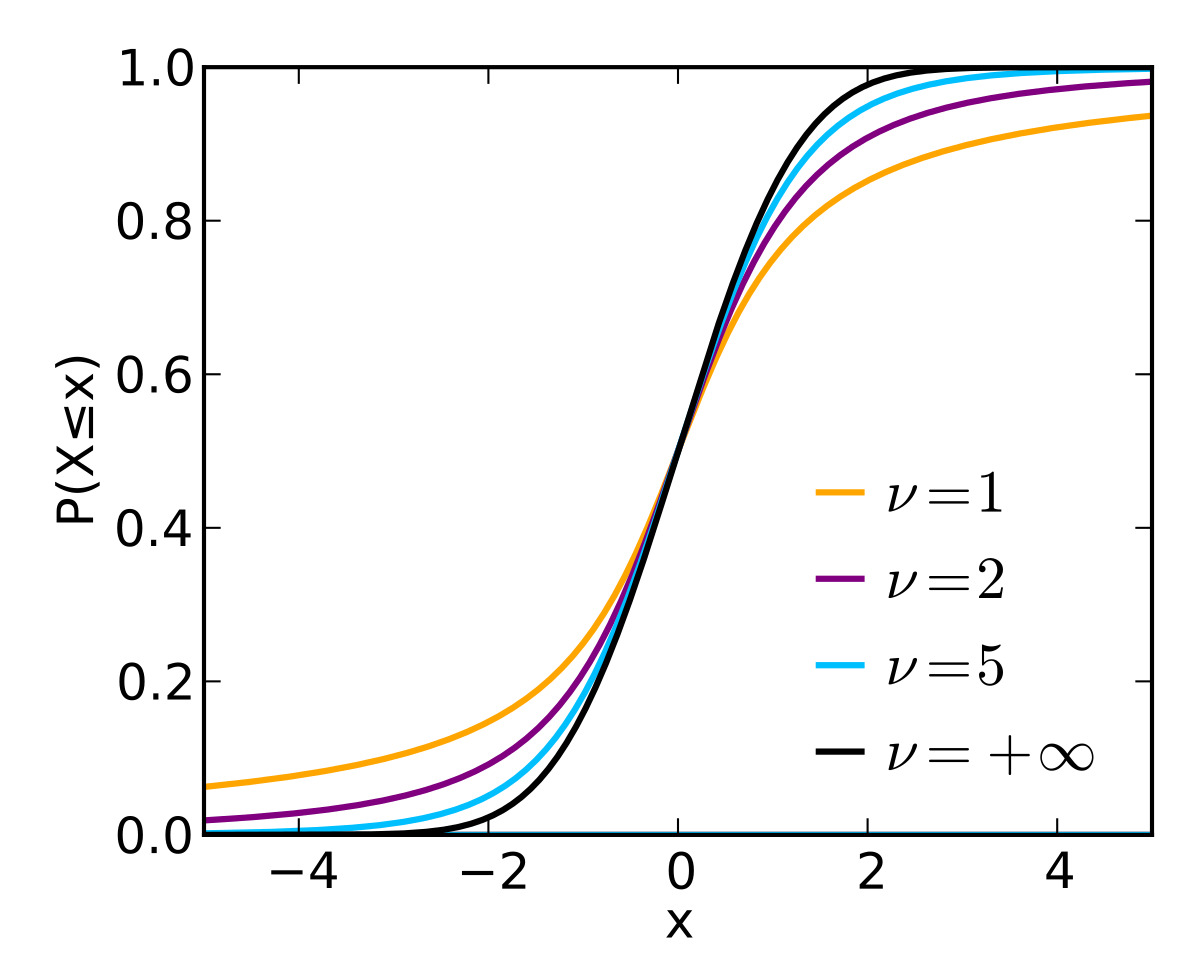
\includegraphics[width=\linewidth, height=4cm, keepaspectratio]{Pictures/distributions/Student_t_cdf.jpg}
            \caption{Student's t-Distribution: CDF}
        \end{figure}
    \end{minipage}
\end{table}

\begin{customTableWrapper}{2}
\begin{longtable}{|m{6cm}|p{9cm}|}
    \hline
    \customTableHeaderColor
    \multicolumn{2}{|c|}{\textbf{Student's t-Distribution - Info} \cite{wiki/Student_t-distribution}} \\
    \hline\endfirsthead

    \hline
    \customTableHeaderColor
    \multicolumn{2}{|c|}{\textbf{Student's t-Distribution - Info - contd.} \cite{wiki/Student_t-distribution}} \\
    \hline\endhead
    
    \hline\endfoot
    \hline\endlastfoot

    \textbf{Statistical parameters} & 
    ${\displaystyle \ \nu >0\ }$ degrees of freedom (real, almost always a positive integer)
    \\ \hline
    
    \textbf{Support} &
    ${\displaystyle \ x\in (-\infty ,\infty )}$
    \\ \hline

    \textbf{Probability Density Function (PDF)} &
    ${\displaystyle \textstyle \ {\dfrac {\Gamma \left({\dfrac {\ \nu +1\ }{2}}\right)}{{\sqrt {\pi \ \nu \ }}\ \Gamma \left({\dfrac {\nu }{\ 2\ }}\right)}}\ \left(\ 1+{\dfrac {~x^{2}\ }{\nu }}\ \right)^{-{\dfrac {\ \nu +1\ }{2}}}\ }$
    \\[2ex] \hline
    
    \textbf{Cumulative distribution function (CDF)} &
    \tableenumerate{
        \item ${\displaystyle {\begin{matrix}\ {\dfrac {\ 1\ }{2}}+x\ \Gamma \left({\dfrac {\ \nu +1\ }{2}}\right)\times \\[0.5em]{\dfrac {\ {{}_{2}F_{1}}\!\left(\ {\dfrac {\ 1\ }{2}},\ {\dfrac {\ \nu +1\ }{2}};\ {\dfrac {3}{\ 2\ }};\ -{\dfrac {~x^{2}\ }{\nu }}\ \right)\ }{\ {\sqrt {\pi \nu }}\ \Gamma \left({\dfrac {\ \nu \ }{2}}\right)\ }}\ \end{matrix}}}$ 

        \item[] where ${\displaystyle \ {}_{2}F_{1}\!(\ ,\ ;\ ;\ )\ }$ is the hypergeometric function
    }
    \\ \hline

    \textbf{Mean} & 
    ${\displaystyle \ 0\ }$ for ${\displaystyle \ \nu >1\ }$, otherwise \textbf{undefined}
    \\[1ex] \hline

    \textbf{Median} & 
    $0$
    \\[1ex] \hline

    \textbf{Mode} & 
    $0$
    \\ \hline

    \textbf{Variance} &
    ${\displaystyle \textstyle \ {\dfrac {\nu }{\ \nu -2\ }}\ }$ for ${\displaystyle \ \nu >2\ }$, $\infty$ for ${\displaystyle \ 1<\nu \leq 2\ }$, otherwise \textbf{undefined}
    \\[1ex] \hline

    \textbf{Skewness} &
    ${\displaystyle \ 0\ }$ for ${\displaystyle \ \nu >3\ }$, otherwise \textbf{undefined}
    \\ \hline

    \textbf{Excess kurtosis} &
    ${\displaystyle \textstyle \ {\dfrac {6}{\ \nu -4\ }}}$ for ${\displaystyle \ \nu >4\ }$, $\infty$ for ${\displaystyle \ 2<\nu \leq 4\ }$, otherwise \textbf{undefined}
    \\[1ex] \hline

    \textbf{Entropy} &
    \tableenumerate{
        \item ${\displaystyle \ {\begin{matrix}{\frac {\ \nu +1\ }{2}}\left[\ \psi \left({\frac {\ \nu +1\ }{2}}\right)-\psi \left({\frac {\ \nu \ }{2}}\right)\ \right]\\[0.5em]+\ln \left[{\sqrt {\nu \ }}\ {\mathrm {B} }\left(\ {\frac {\ \nu \ }{2}},\ {\frac {\ 1\ }{2}}\ \right)\right]\ {\scriptstyle {\text{(nats)}}}\ \end{matrix}}}$

        \item[] where
        \begin{enumerate}
            \item[] ${\displaystyle \psi ()\ }$ is the digamma function
            
            \item[] ${\displaystyle \ {\mathrm {B} }(\ ,\ )\ }$ is the beta function.
        \end{enumerate}
    }
    \\[1ex] \hline

    \textbf{Moment-generating function (MGF)} &
    undefined
    \\[1ex] \hline

    \textbf{Characteristic function (CF)} &
    \tableenumerate{
        \item ${\displaystyle \textstyle {\dfrac {\ \left(\ {\sqrt {\nu \ }}\ \dabs{t}\ \right)^{\nu /2}\ K_{\nu /2}\left(\ {\sqrt {\nu \ }}\ \dabs{t}\ \right)\ }{\ \Gamma (\nu /2)\ 2^{\nu /2-1}\ }}\ }$ for ${\displaystyle \ \nu >0\ }$
        
        \item[] ${\displaystyle \ K_{\nu }(x)\ }$ is the modified Bessel function of the second kind
    }
    \\[1ex] \hline

    \textbf{Expected shortfall} &
    \tableenumerate{
        \item ${\displaystyle \ \mu +s\ \left(\ {\frac {\ \nu +T^{-1}(1-p)^{2}\ \times \ \tau \left(T^{-1}(1-p)^{2}\right)\ }{\ (\nu -1)(1-p)\ }}\ \right)\ }$

        \item[] Where: 
        \begin{enumerate}
            \item ${\displaystyle \ T^{-1}(\ )\ }$ is the inverse standardized Student t CDF
            \item ${\displaystyle \ \tau (\ )\ }$ is the standardized Student t PDF
        \end{enumerate}
    }
    \\[1ex] \hline


\end{longtable}
\end{customTableWrapper}

\begin{enumerate}
    \item if $Z \sim \mathcal{N}(0,1)$ and $V_n^2 \sim \chi_n^2$ and $Z$ and $V_n^2$ are independent, $Z/(V_n/\sqrt{n})$ has a student t distribution

    \item Properties:
    \begin{enumerate}
        \item $x_p(f_t) = -x_{1-p}(f_t)$

    \end{enumerate}

    \item Confidence Interval:
    \begin{enumerate}
        \item If $x_p(f_t)$ is the $p$th quantile of the Student t-distribution with $n - 1$ degrees of freedom, the $1 - 2p$ confidence interval for $\mu$ (with $p < 0.5$) is:
        \[\left(
            \bar{X} - x_{1-p}(f_t)\dfrac{S}{\sqrt{n}},
            \hspace{0.2cm}
            \bar{X} + x_{1-p}(f_t)\dfrac{S}{\sqrt{n}}
        \right]\]

    \end{enumerate}

\end{enumerate}






















































\chapter{Gamma Distribution ($X \sim G(\alpha, \beta)/ G(k,\theta)$) \cite{ism-1,wiki/Gamma_distribution}}\label{Gamma Distribution}

\begin{table}[H]
    \begin{minipage}{0.49\linewidth}
        \begin{figure}[H]
            \centering
            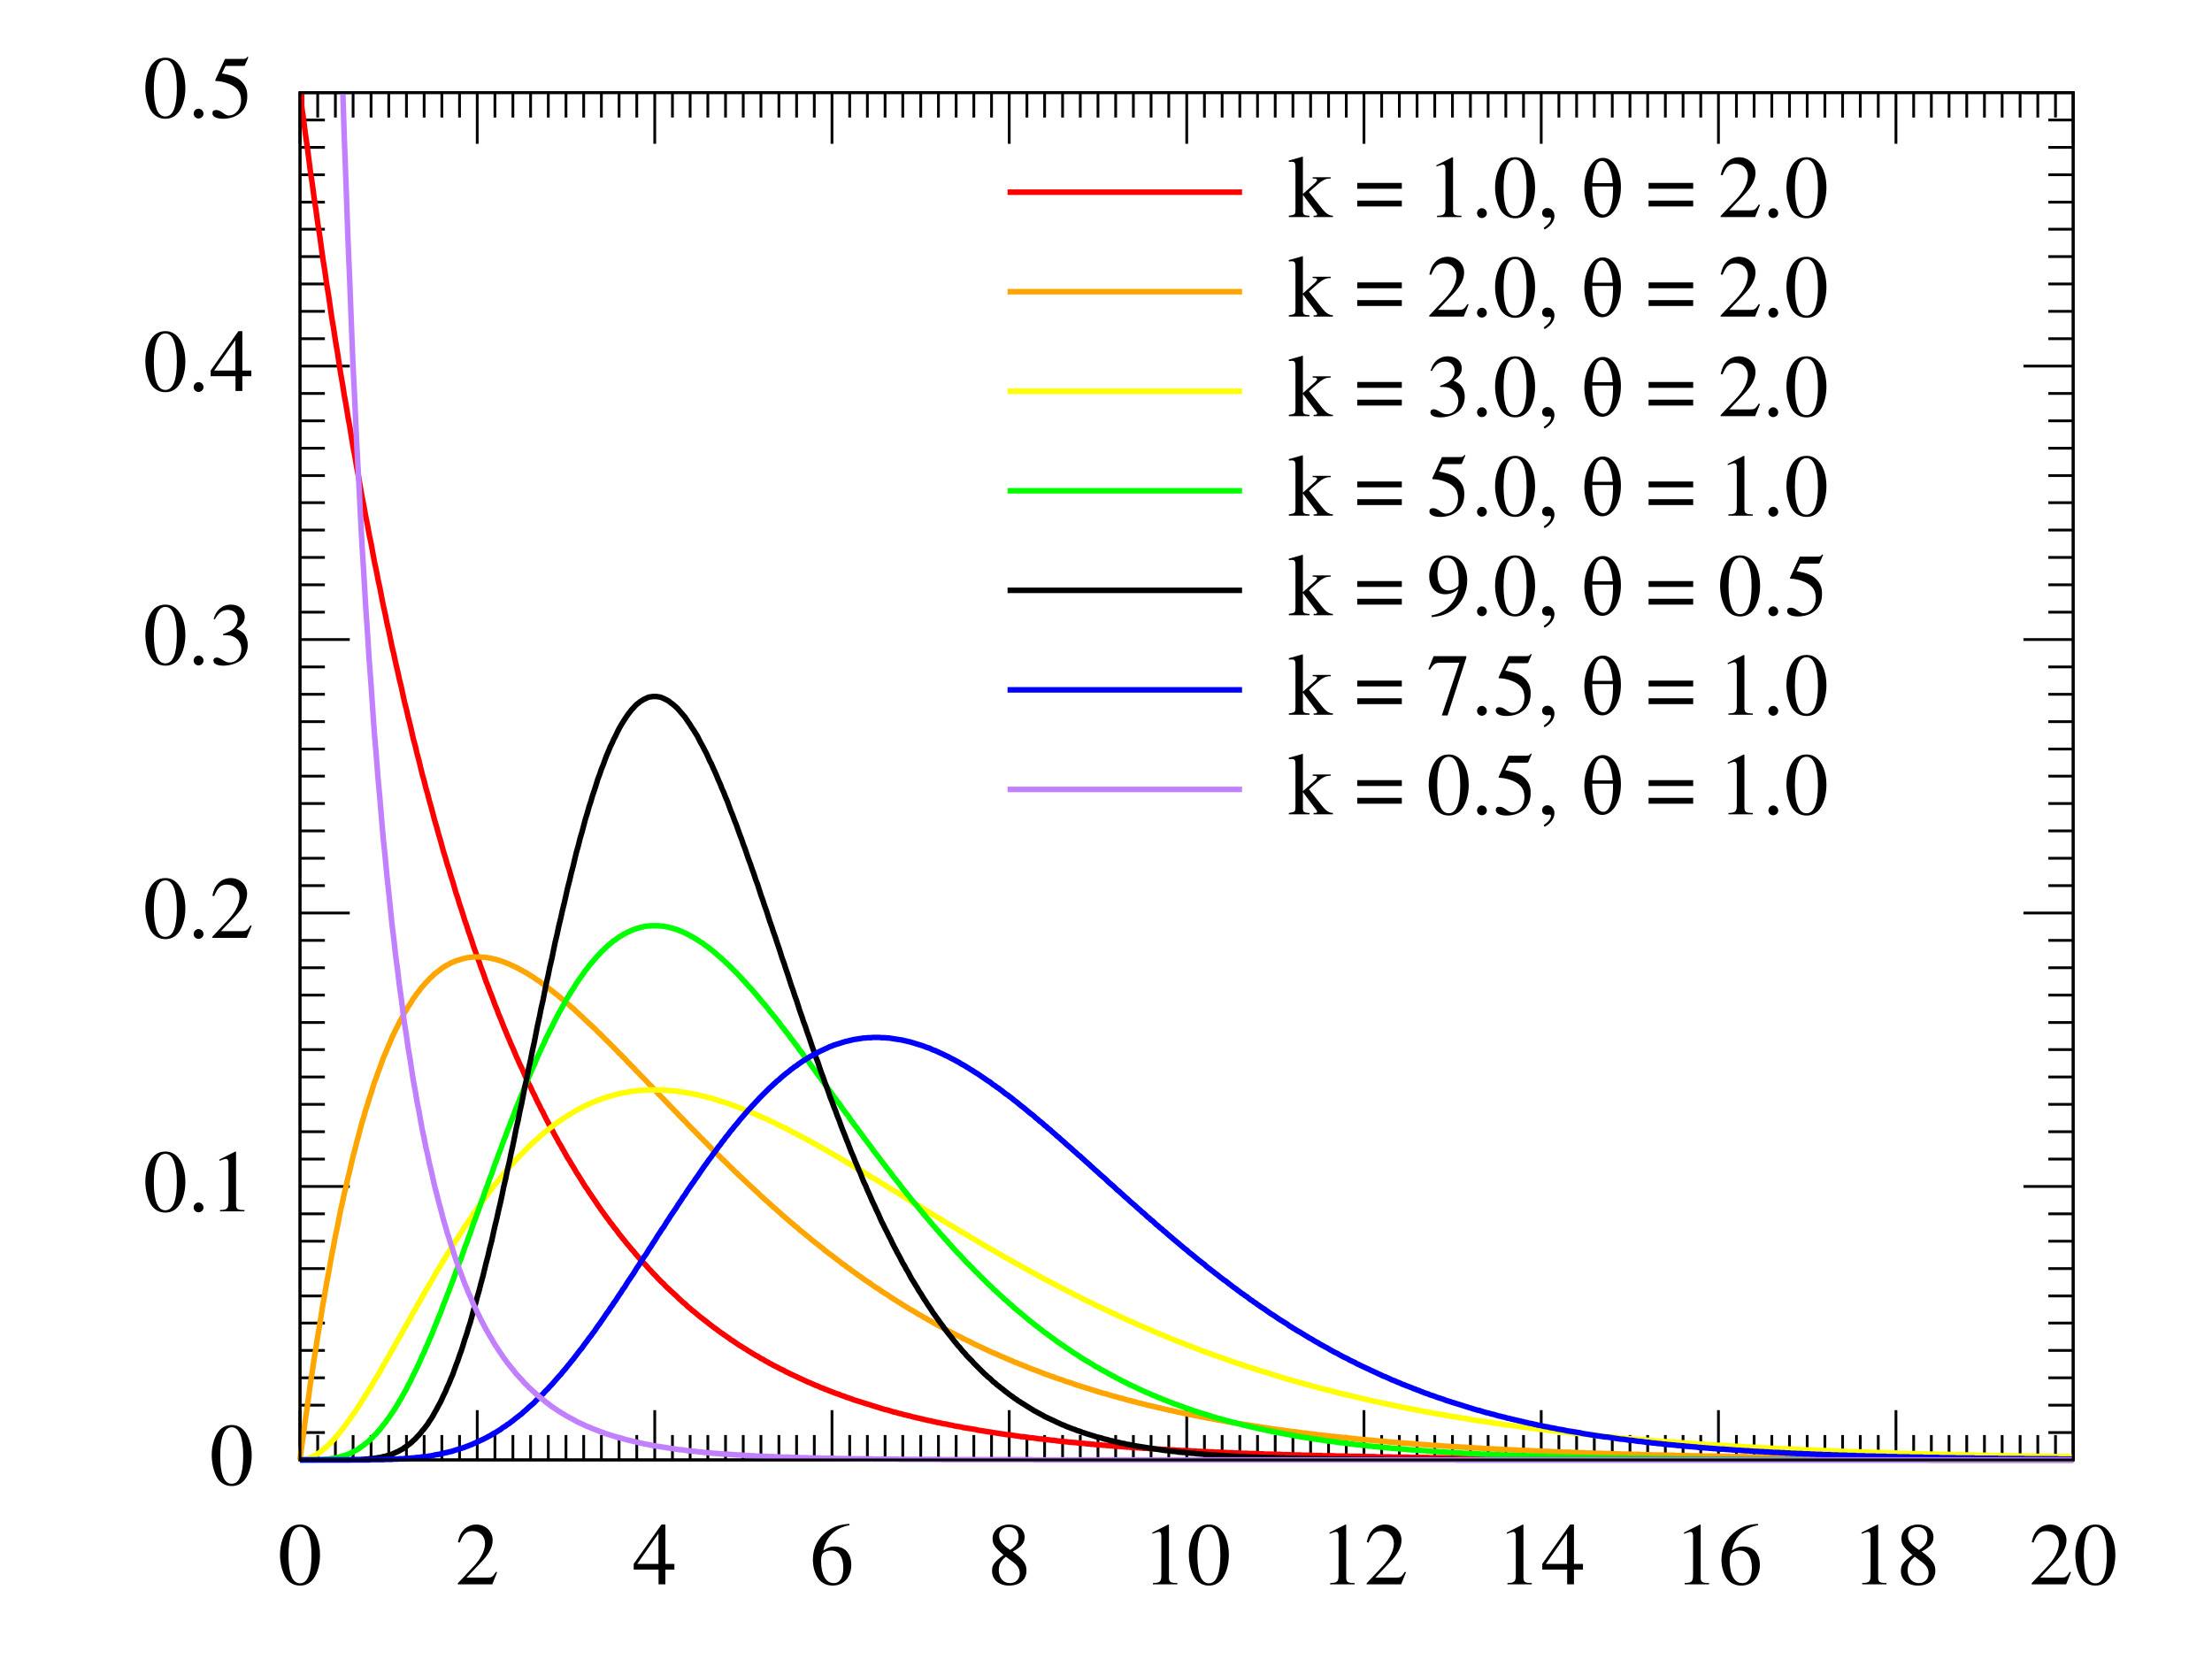
\includegraphics[width=\linewidth, height=4cm, keepaspectratio]{Pictures/distributions/Gamma_distribution_pdf.jpg}
            \caption{Gamma distribution: PDF}
        \end{figure}
    \end{minipage}
    \hfill
    \begin{minipage}{0.49\linewidth}
        \begin{figure}[H]
            \centering
            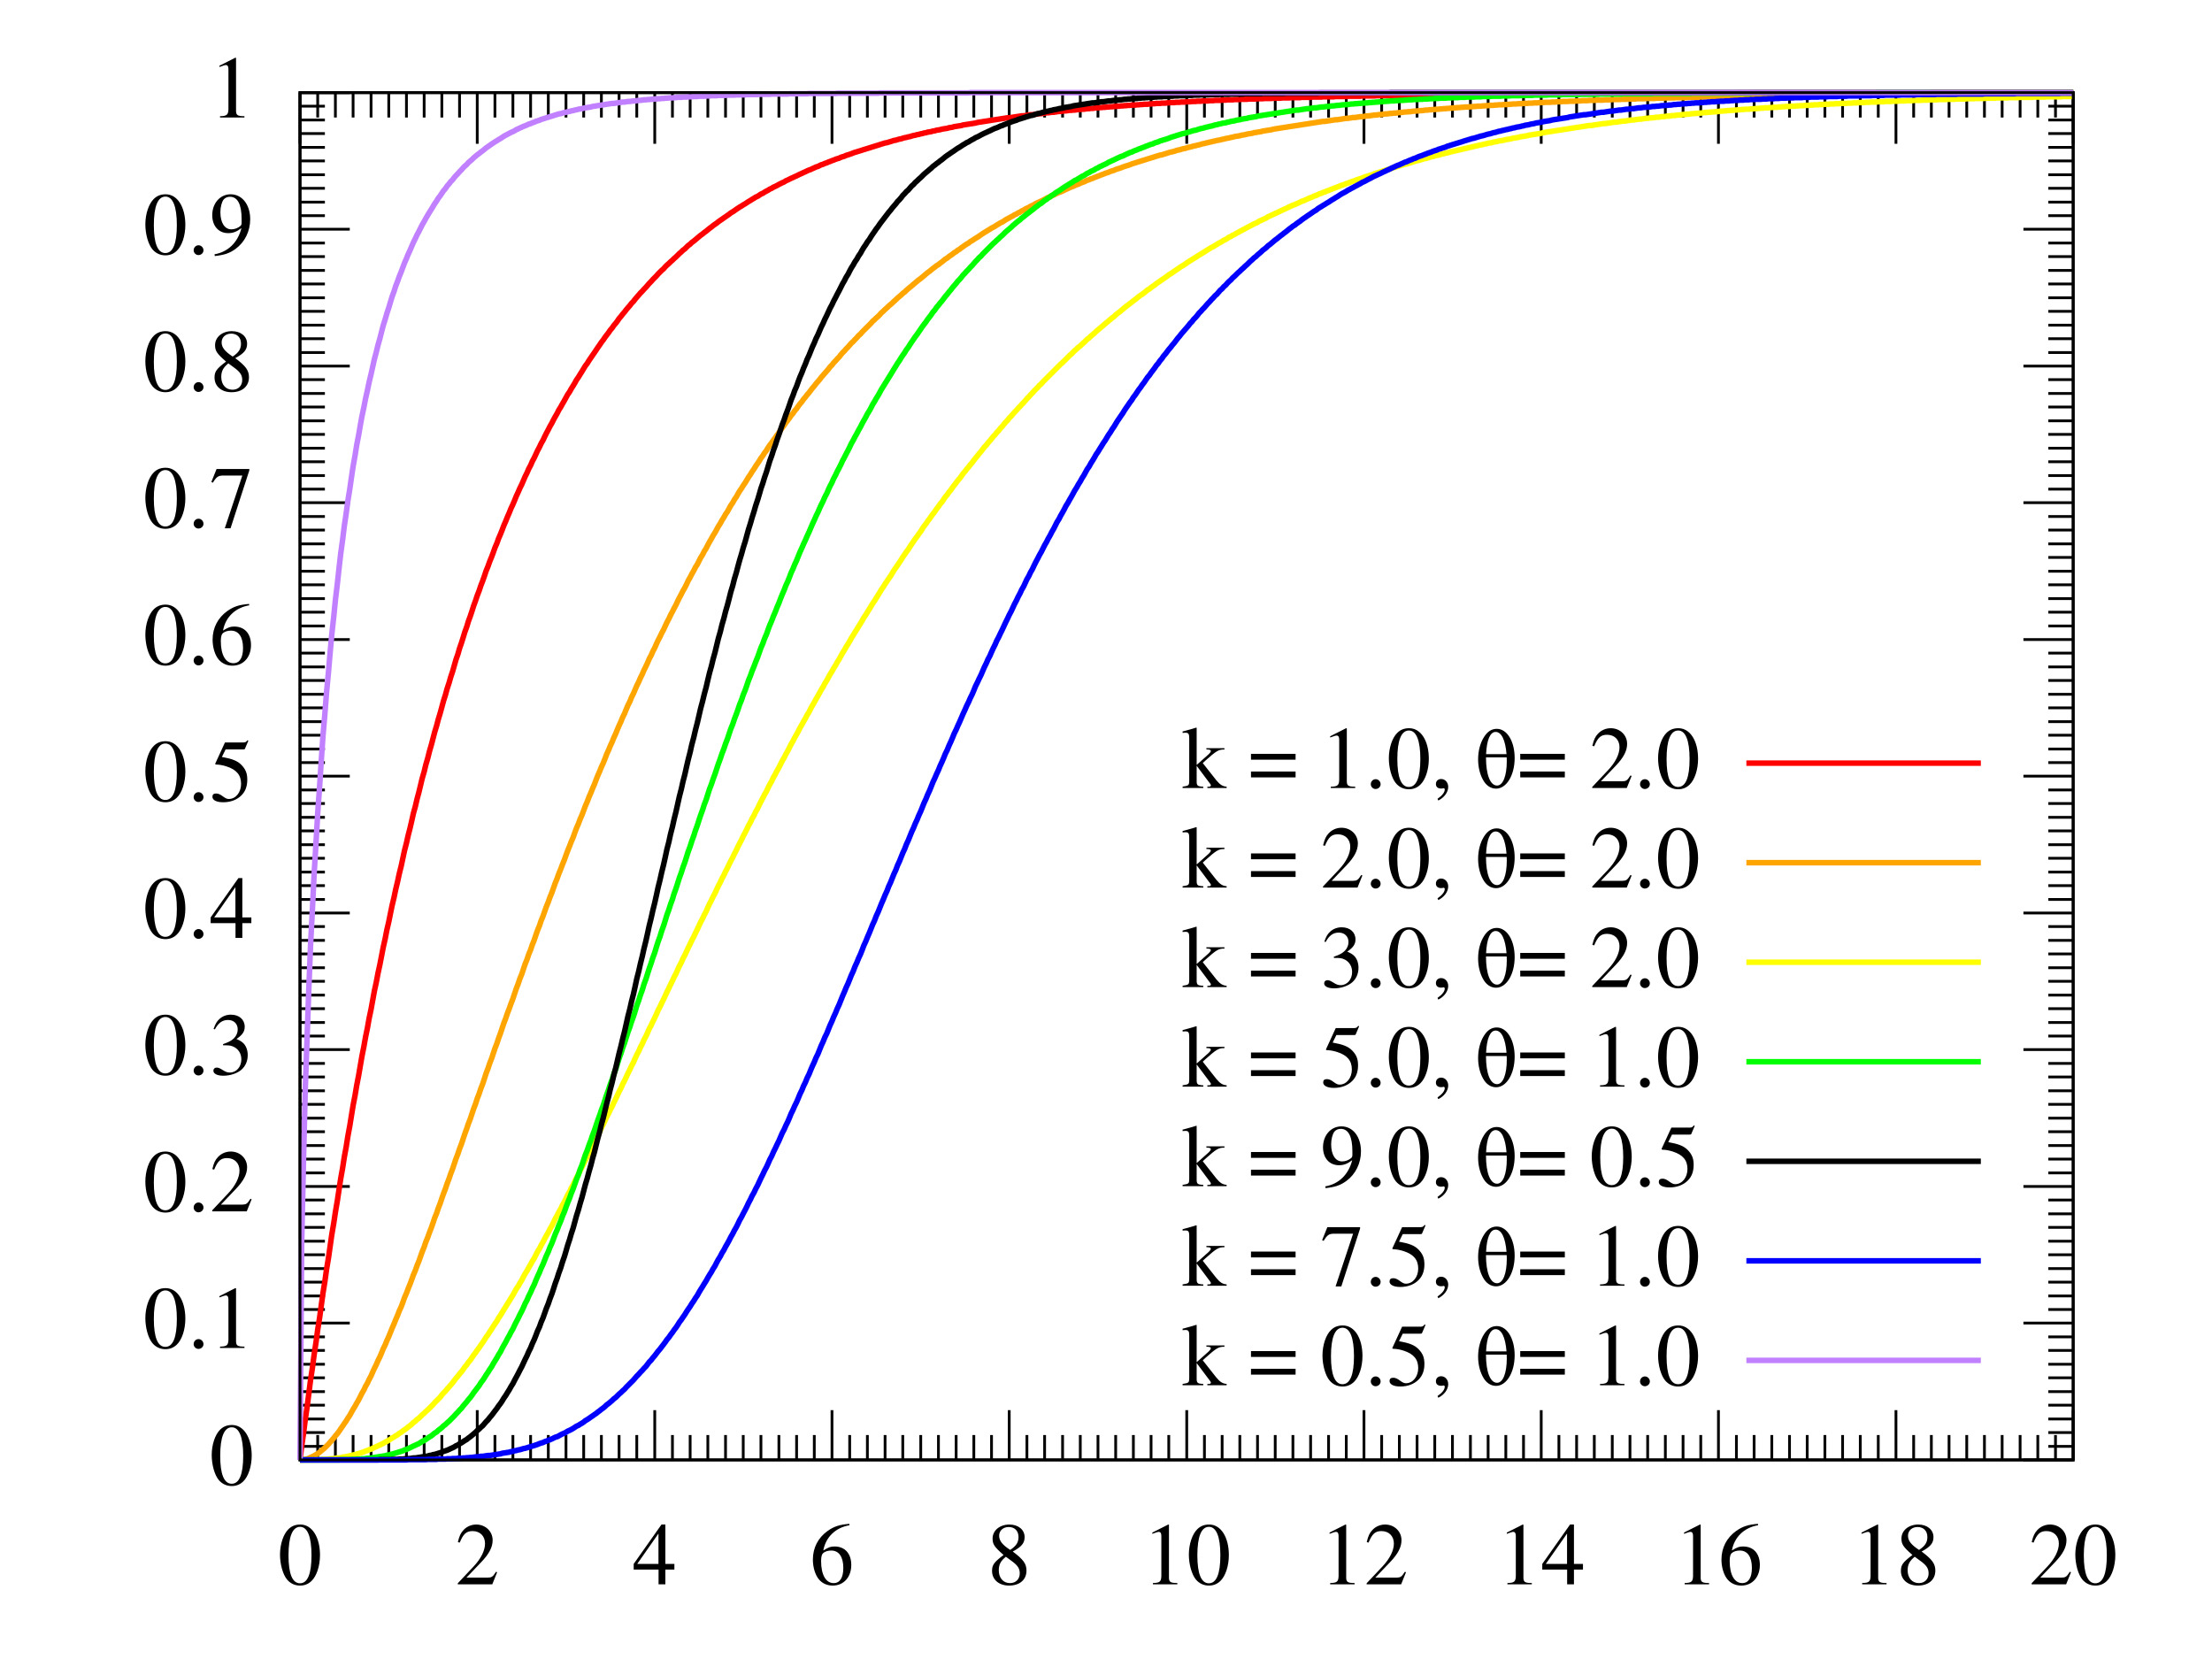
\includegraphics[width=\linewidth, height=4cm, keepaspectratio]{Pictures/distributions/Gamma_distribution_cdf.jpg}
            \caption{Gamma distribution: CDF}
        \end{figure}
    \end{minipage}
\end{table}

\begin{customTableWrapper}{2}
\begin{longtable}{|m{3cm}|p{5.5cm}|p{5.5cm}|}
    \hline
    \customTableHeaderColor
    \multicolumn{3}{|c|}{\textbf{Gamma Distribution - Info} \cite{wiki/Exponential_distribution}} \\ \hline
    & $G(k,\theta)$ & $G(\alpha, \beta)$ \\
    \hline\endfirsthead

    \hline
    \customTableHeaderColor
    \multicolumn{3}{|c|}{\textbf{Gamma Distribution - Info - contd.} \cite{wiki/Exponential_distribution}} \\ \hline
    & $G(k,\theta)$ & $G(\alpha, \beta)$ \\
    \hline\endhead
    
    \hline\endfoot
    \hline\endlastfoot

    \textbf{Statistical parameters} & 
    \tableenumerate{
        \item $k > 0$ shape
        \item $\theta > 0$ scale
    } &
    \tableenumerate{
        \item $\alpha > 0$ shape
        \item $\beta > 0$ rate
    }
    \\ \hline
    
    \textbf{Support} &
    \multicolumn{2}{|c|}{${ x\in (0,\infty )}$}
    \\ \hline

    \textbf{Probability Density Function (PDF)} & 
    ${ f(x)={\dfrac {1}{\Gamma (k)\theta ^{k}}}x^{k-1}e^{-x/\theta }}$ &
    ${ f(x)={\dfrac {\beta ^{\alpha }}{\Gamma (\alpha )}}x^{\alpha -1}e^{-\beta x}}$
    \\[1ex] \hline
    
    \textbf{Cumulative distribution function (CDF)} & 
    ${ F(x)={\dfrac {1}{\Gamma (k)}}\gamma \left(k,{\dfrac {x}{\theta }}\right)}$ &
    ${ F(x)={\dfrac {1}{\Gamma (\alpha )}}\gamma (\alpha ,\beta x)}$
    \\ \hline

    \textbf{Mean} & 
    ${ k\theta }$ &
    ${ {\dfrac {\alpha }{\beta }}}$
    \\[1ex] \hline

    \textbf{Median} & 
    \multicolumn{2}{|c|}{No simple closed form}
    \\[1ex] \hline

    \textbf{Mode} & 
    \tableenumerate{
        \item ${ (k-1)\theta {\text{ for }}k\geq 1}$ 
        \item ${ 0{\text{ for }}k<1}$
    } &
    ${ {\dfrac {\alpha -1}{\beta }}{\text{ for }}\alpha \geq 1{\text{, }}0{\text{ for }}\alpha <1}$
    \\ \hline

    \textbf{Variance} &
    ${ k\theta ^{2}}$ &
    ${ {\dfrac {\alpha }{\beta ^{2}}}}$
    \\[1ex] \hline

    \textbf{Skewness} &
    ${ {\dfrac {2}{\sqrt {k}}}}$&
    ${ {\dfrac {2}{\sqrt {\alpha }}}}$
    \\[1ex] \hline

    \textbf{Excess kurtosis} &
    ${ {\dfrac {6}{k}}}$&
    ${ {\dfrac {6}{\alpha }}}$
    \\[1ex] \hline

    \textbf{Entropy} &
    ${ {\begin{aligned}k&+\ln \theta +\ln \Gamma (k)\\&+(1-k)\psi (k)\end{aligned}}}$&
    ${ {\begin{aligned}\alpha &-\ln \beta +\ln \Gamma (\alpha )\\&+(1-\alpha )\psi (\alpha )\end{aligned}}}$
    \\[1ex] \hline

    \textbf{Moment-generating function (MGF)} &
    ${ (1-\theta t)^{-k}{\text{ for }}t<{\dfrac {1}{\theta }}}$&
    ${ \left(1-{\dfrac {t}{\beta }}\right)^{-\alpha }{\text{ for }}t<\beta }$
    \\[1ex] \hline

    \textbf{Characteristic function (CF)} &
    ${ (1-\theta it)^{-k}}$&
    ${ \left(1-{\dfrac {it}{\beta }}\right)^{-\alpha }}$
    \\[1ex] \hline

    \textbf{Fisher information} &
    ${ I(k,\theta )={\begin{pmatrix}\psi ^{(1)}(k)&\theta ^{-1}\\\theta ^{-1}&k\theta ^{-2}\end{pmatrix}}}$&
    ${ I(\alpha ,\beta )={\begin{pmatrix}\psi ^{(1)}(\alpha )&-\beta ^{-1}\\-\beta ^{-1}&\alpha \beta ^{-2}\end{pmatrix}}}$
    \\[1ex] \hline

    \textbf{Method of moments} &
    $
        { k={\dfrac {E[X]^{2}}{V[X]}}\quad \quad }
        \quad\quad
        { \theta ={\dfrac {V[X]}{E[X]}}\quad \quad }
    $&
    $
        { \alpha ={\dfrac {E[X]^{2}}{V[X]}}}
        \quad\quad
        { \beta ={\dfrac {E[X]}{V[X]}}}
    $
    \\[1ex] \hline

\end{longtable}
\end{customTableWrapper}

\begin{enumerate}
    \item here are two equivalent parameterizations in common use:
    \begin{enumerate}
        \item With a shape parameter $k$ and a scale parameter $\theta$

        \item With a shape parameter ${ \alpha =k}$ and an inverse scale parameter ${ \beta =1/\theta }$, called a rate parameter.

    \end{enumerate}

\end{enumerate}






































\chapter{Beta Distribution ($Beta(\alpha, \beta)$) \cite{ism-1,wiki/Beta_distribution,mfml-1}} \label{Beta Distribution}


\begin{table}[H]
    \begin{minipage}{0.49\linewidth}
        \begin{figure}[H]
            \centering
            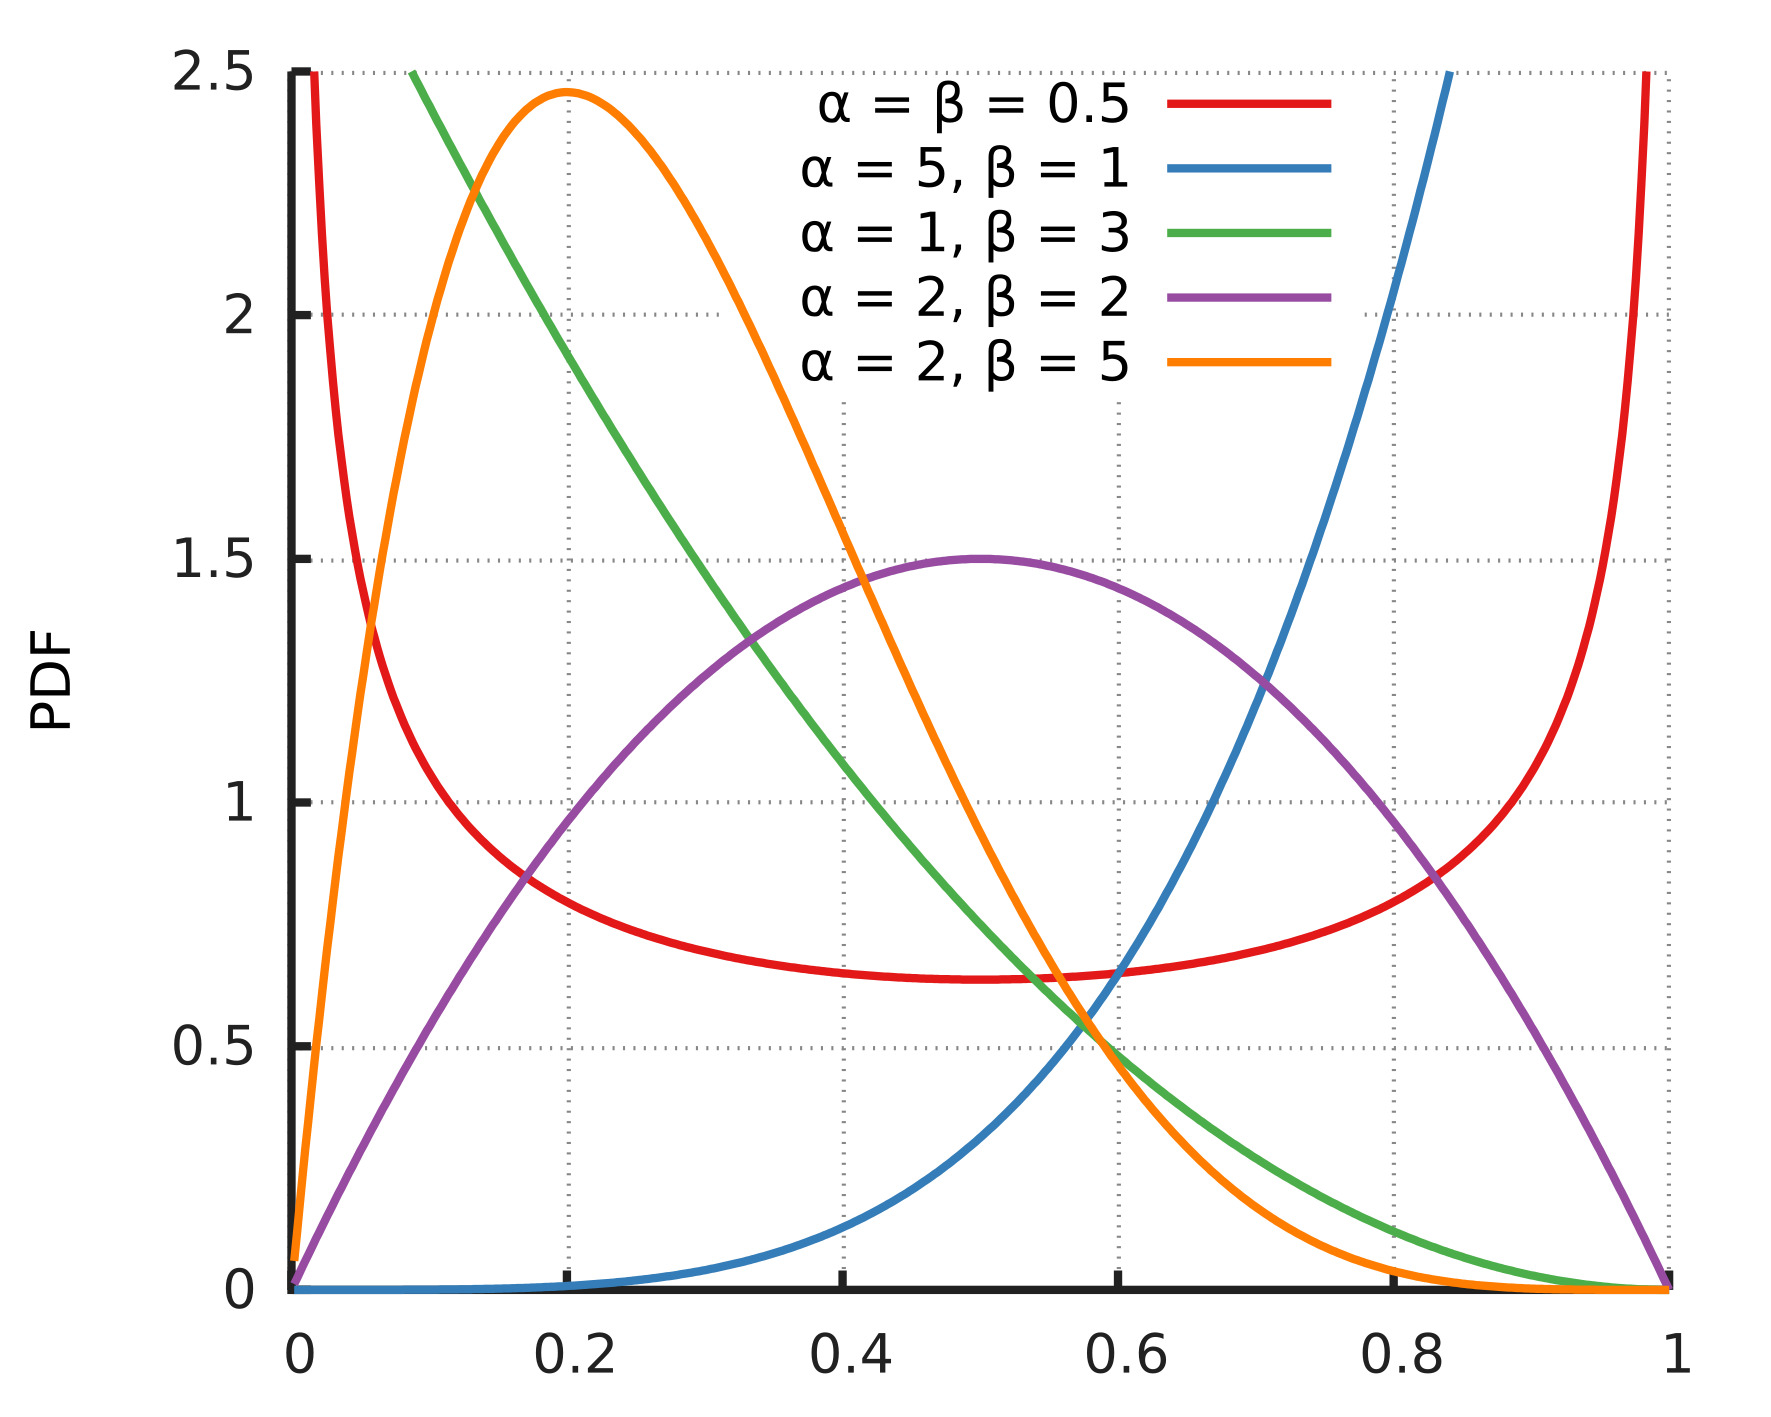
\includegraphics[width=\linewidth, height=4cm, keepaspectratio]{Pictures/distributions/Beta_distribution_pdf.jpg}
            \caption{Beta Distribution: PDF}
        \end{figure}
    \end{minipage}
    \hfill
    \begin{minipage}{0.49\linewidth}
        \begin{figure}[H]
            \centering
            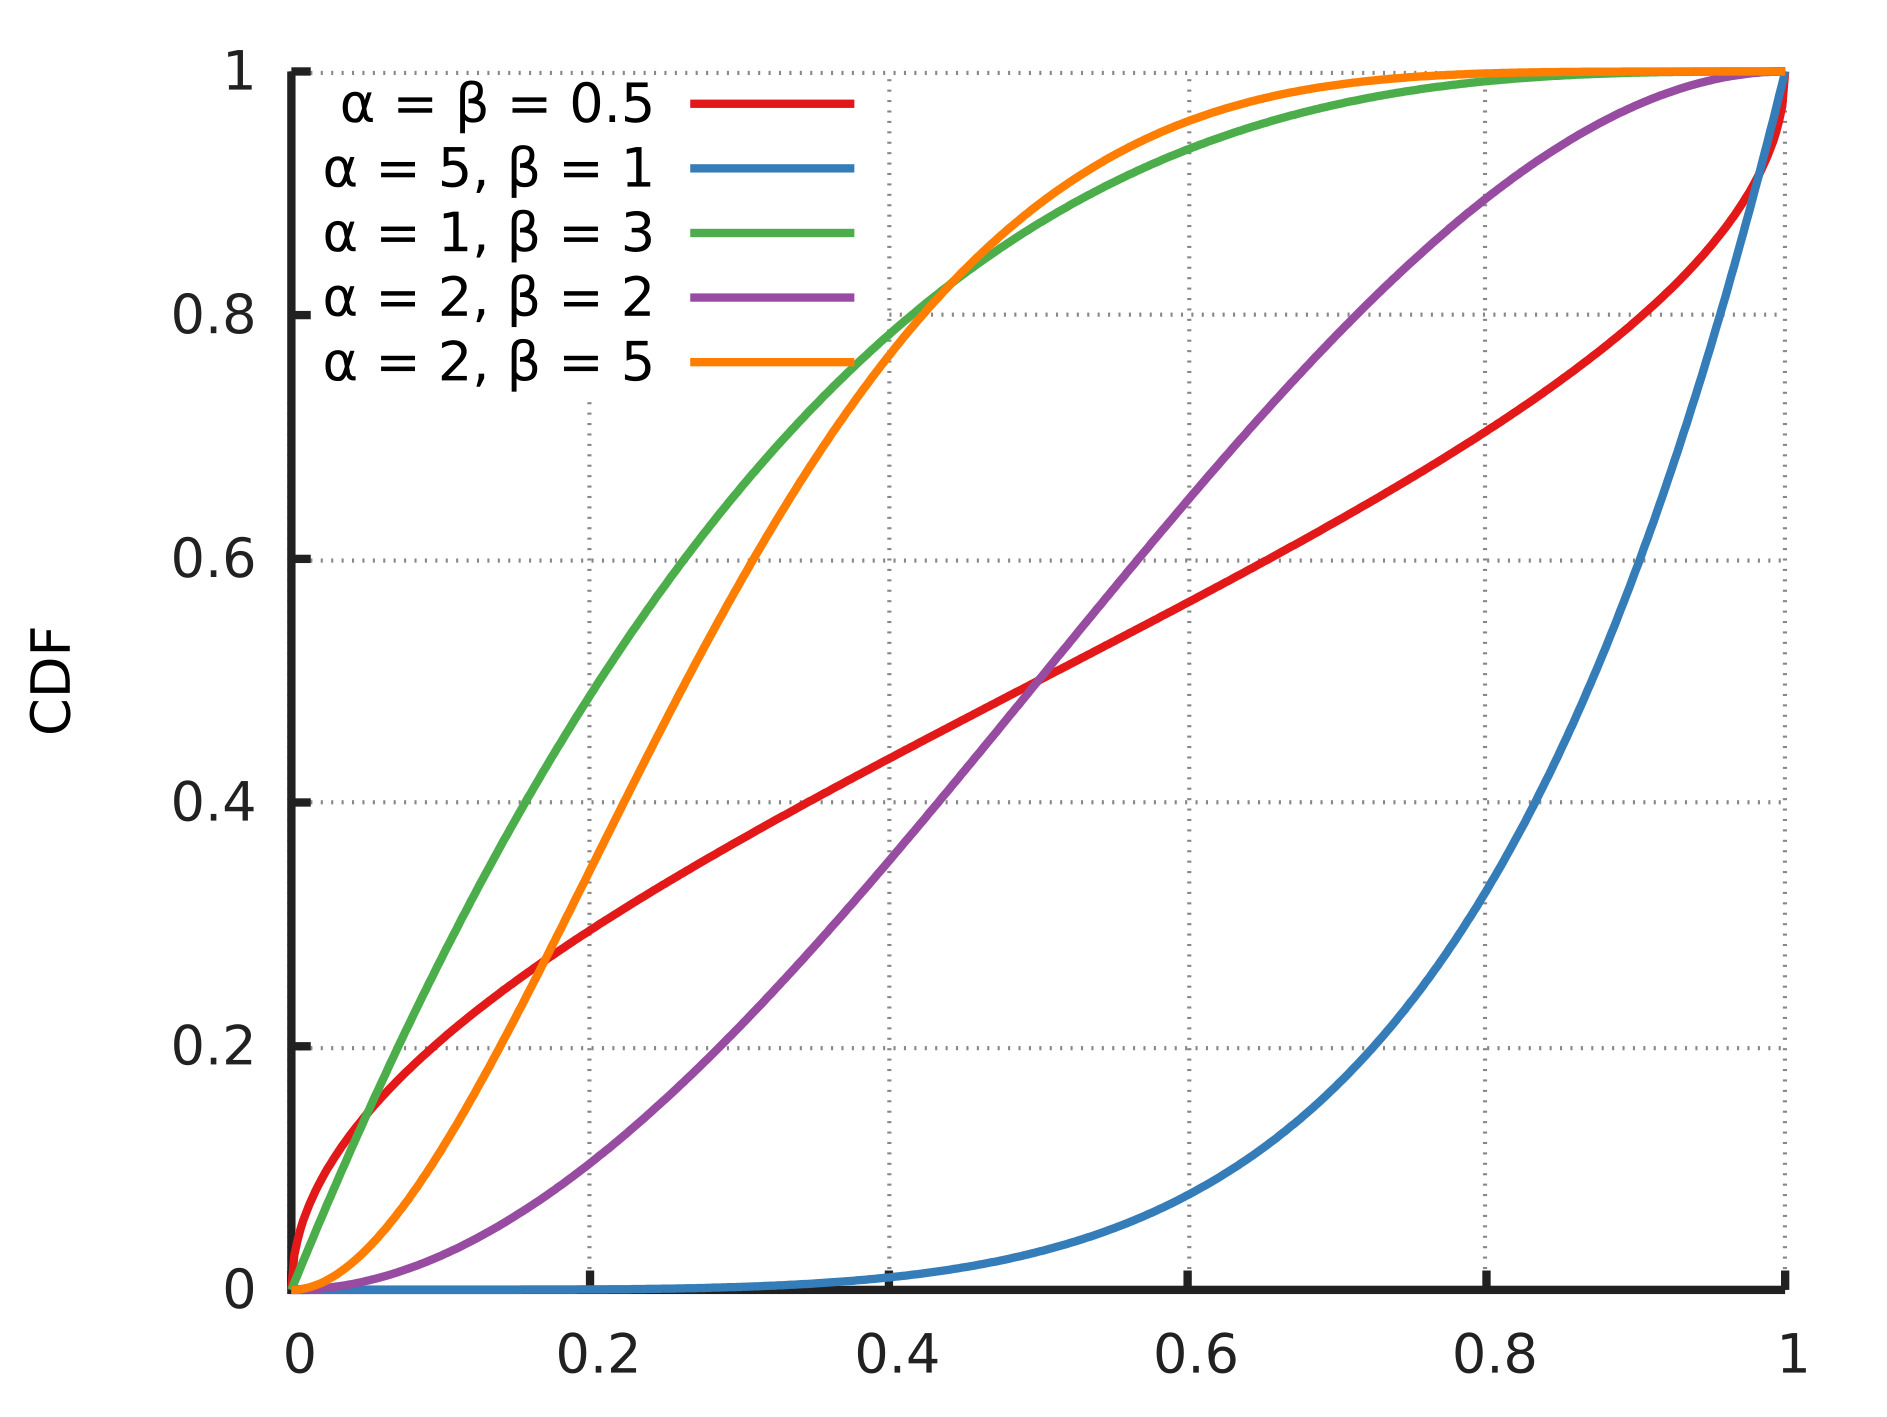
\includegraphics[width=\linewidth, height=4cm, keepaspectratio]{Pictures/distributions/Beta_distribution_cdf.jpg}
            \caption{Beta Distribution: CDF}
        \end{figure}
    \end{minipage}
\end{table}

\begin{customTableWrapper}{2}
\begin{longtable}{|m{6cm}|p{9cm}|}
    \hline
    \customTableHeaderColor
    \multicolumn{2}{|c|}{\textbf{Beta Distribution - Info} \cite{wiki/Beta_distribution}} \\
    \hline\endfirsthead

    \hline
    \customTableHeaderColor
    \multicolumn{2}{|c|}{\textbf{Beta Distribution - Info - contd.} \cite{wiki/Beta_distribution}} \\
    \hline\endhead
    
    \hline\endfoot
    \hline\endlastfoot

    \textbf{Statistical parameters} & 
    \tableenumerate{
        \item $\alpha > 0$ shape (real)
        \item $\beta > 0$ shape (real)
    }
    \\[1ex] \hline
    
    \textbf{Support} &
    ${ x\in [0,1]\!}$ or ${ x\in (0,1)\!}$
    \\[1ex] \hline

    \textbf{Probability Density Function (PDF)} & 
    \tableenumerate{
        \item[] ${ {\dfrac {x^{\alpha -1}(1-x)^{\beta -1}}{\mathrm {B} (\alpha ,\beta )}}\!}$
        
        \item[] where ${ \mathrm {B} (\alpha ,\beta )={\dfrac {\Gamma (\alpha )\Gamma (\beta )}{\Gamma (\alpha +\beta )}}}$ and ${ \Gamma }$ is the Gamma function.
    }
    \\[1ex] \hline
    
    \textbf{Cumulative distribution function (CDF)} & 
    ${ I_{x}(\alpha ,\beta )\!}$
    \\[1ex] \hline

    \textbf{Mean} & 
    \tableenumerate{
        \item ${ \operatorname {E} [X]={\dfrac {\alpha }{\alpha +\beta }}\!}$

        \item ${ \operatorname {E} [\ln X]=\psi (\alpha )-\psi (\alpha +\beta )\!}$

        \item ${ \operatorname {E} [X\,\ln X]={\dfrac {\alpha }{\alpha +\beta }}\,\left[\psi (\alpha +1)-\psi (\alpha +\beta +1)\right]\!}$

        \item[] where ${ \psi }$ is the digamma function
    }
    \\[1ex] \hline

    \textbf{Median} & 
    ${ {\begin{matrix}I_{\dfrac {1}{2}}^{[-1]}(\alpha ,\beta ){\text{ (in general) }}\\[0.5em]\approx {\dfrac {\alpha -{\dfrac {1}{3}}}{\alpha +\beta -{\dfrac {2}{3}}}}{\text{ for }}\alpha ,\beta >1\end{matrix}}}$
    \\[1ex] \hline

    \textbf{Mode} & 
    \tableenumerate{
        \item ${ {\dfrac {\alpha -1}{\alpha +\beta -2}}\!}$ for $\alpha, \beta > 1$

        \item any value in ${ (0,1)}$ for $\alpha, \beta = 1$

        \item $\dCurlyBrac{0, 1}$ (bimodal) for $\alpha, \beta < 1$

        \item $0$ for $\alpha \leq 1, \beta \geq 1, \alpha \neq \beta$

        \item $1$ for $\alpha \geq 1, \beta \leq 1, \alpha \neq \beta$
    }
    \\[1ex] \hline

    \textbf{Variance} &
    \tableenumerate{
        \item ${ \operatorname {var} [X]={\dfrac {\alpha \beta }{(\alpha +\beta )^{2}(\alpha +\beta +1)}}\!}$

        \item ${ \operatorname {var} [\ln X]=\psi _{1}(\alpha )-\psi _{1}(\alpha +\beta )\!}$
    }
    \\[1ex] \hline

    \textbf{Mean absolute deviation (MAD)} &
    \\[1ex] \hline

    \textbf{Skewness} &
    ${ {\dfrac {2\,(\beta -\alpha ){\sqrt {\alpha +\beta +1}}}{(\alpha +\beta +2){\sqrt {\alpha \beta }}}}}$
    \\[1ex] \hline

    \textbf{Excess kurtosis} &
    ${ {\dfrac {6[(\alpha -\beta )^{2}(\alpha +\beta +1)-\alpha \beta (\alpha +\beta +2)]}{\alpha \beta (\alpha +\beta +2)(\alpha +\beta +3)}}}$
    \\[1ex] \hline

    \textbf{Entropy} &
    ${ {\begin{matrix}\ln \mathrm {B} (\alpha ,\beta )-(\alpha -1)\psi (\alpha )-(\beta -1)\psi (\beta )\\[0.5em]{}+(\alpha +\beta -2)\psi (\alpha +\beta )\end{matrix}}}$
    \\[1ex] \hline

    \textbf{Moment-generating function (MGF)} &
    ${ 1+\sum _{k=1}^{\infty }\left(\prod _{r=0}^{k-1}{\dfrac {\alpha +r}{\alpha +\beta +r}}\right){\dfrac {t^{k}}{k!}}}$
    \\[1ex] \hline

    \textbf{Characteristic function (CF)} &
    ${ {}_{1}F_{1}(\alpha ;\alpha +\beta ;i\,t)\!}$ (see Confluent hypergeometric function)
    \\[1ex] \hline

    \textbf{Fisher information} &
    ${ {\begin{bmatrix}\operatorname {var} [\ln X]&\operatorname {cov} [\ln X,\ln(1-X)]\\\operatorname {cov} [\ln X,\ln(1-X)]&\operatorname {var} [\ln(1-X)]\end{bmatrix}}}$
    \\[1ex] \hline

    \textbf{Method of moments} &
    \tableenumerate{
        \item ${ \alpha =\left({\dfrac {E[X](1-E[X])}{V[X]}}-1\right)E[X]}$
        \vspace{0.1cm}

        \item ${ \beta =\left({\dfrac {E[X](1-E[X])}{V[X]}}-1\right)(1-E[X])}$
        \vspace{0.2cm}
    }
    \\[2ex] \hline

\end{longtable}
\end{customTableWrapper}

\begin{enumerate}
    \item considered a \textbf{conjugate prior distribution}

    \item if $\alpha = 1$ and $\beta = 1$, the resulting beta distribution function is actually a \textbf{uniform distribution} function on $[0, 1]$ \cite{ism-1}

    \item For $\alpha, \beta < 1$, we get a \textbf{bimodal distribution} with spikes at $0$ and $1$. \cite{mfml-1}

    \item For $\alpha, \beta > 1$, the distribution is \textbf{unimodal}. \cite{mfml-1}

    \item For $\alpha, \beta > 1$ and $\alpha = \beta$, the distribution is \textbf{unimodal, symmetric}, and centered in the interval $[0, 1]$, i.e., the mode/mean is at $1/2$. \cite{mfml-1}
\end{enumerate}

\section{Bayesian Analysis \cite{ism-1}} \label{Beta Distribution: Bayesian Analysis}

\begin{enumerate}
    \item Posterior: \cite{ism-1}
    \[
    \begin{aligned}
         f(\theta|x) 
         &\propto p(x|\theta) f (\theta) \\
         &= \theta^{\sum^{n}_{i=1} x_i} 
            (1 - \theta)^{n - \sum^{n}_{i=1} x_i}
            \dfrac{\Gamma (\alpha + \beta)}{\Gamma (\alpha)\Gamma (\beta)}
            \theta^{\alpha-1} (1 - \theta)^{\beta-1} \\
        &\propto \theta^{(\alpha + \sum^{n}_{i=1} x_i)-1} 
            (1-\theta)^{(\beta + n - \sum^{n}_{i=1} x_i)-1} 
    \end{aligned}
    \]

    \begin{enumerate}
        \item[] posterior $f (\theta|D)$ is proportional to the density of a $beta(\alpha', \beta')$ distribution:
        \begin{enumerate}
            \item $\alpha' = \alpha + \dsum^{n}_{i=1} xi$

            \item $\beta' = \beta + n - \dsum^{n}_{i=1} xi$
        
        \end{enumerate}

    \end{enumerate}

    \item Prior:
    \begin{enumerate}
        \item $\alpha$ specifies the a-priori number of \textbf{successes}

        \item $\beta$ specifies the a-priori number of \textbf{failures}

    \end{enumerate}

\end{enumerate}









%%%%%%%%%%%%%%%%%%%%%%%%%%%%%%%%%%%%%%%%%%%%%%%%%%%%%%%%%%%%%%%%%%%%%%%%%%%%%%%%%%%%%%%%%%%%


\chapter{Bernoulli Distribution ($X \sim \mathcal{B}(p)$) \cite{ism-1,wiki/Bernoulli_distribution}}\label{Bernoulli Distribution}


\begin{customTableWrapper}{2}
\begin{longtable}{|m{6cm}|p{9cm}|}
    \hline
    \customTableHeaderColor
    \multicolumn{2}{|c|}{\textbf{Bernoulli Distribution - Info} \cite{wiki/Bernoulli_distribution}} \\
    \hline\endfirsthead

    \hline
    \customTableHeaderColor
    \multicolumn{2}{|c|}{\textbf{Bernoulli Distribution - Info - contd.} \cite{wiki/Bernoulli_distribution}} \\
    \hline\endhead
    
    \hline\endfoot
    \hline\endlastfoot

    \hline

    \textbf{Statistical parameters} & 
    ${\displaystyle 0\leq p\leq 1} \quad {\displaystyle q=1-p}$
    \\ \hline
    
    \textbf{Support} & 
    ${\displaystyle k\in \{0,1\}}$
    \\ \hline

    \textbf{Probability Density Function (PDF)} & 
    ${\displaystyle {\begin{dcases}q=1-p&{\text{if }}k=0\\p&{\text{if }}k=1\end{dcases}}}$
    \\[2ex] \hline
    
    \textbf{Cumulative distribution function (CDF)} & 
    ${\displaystyle {\begin{dcases}0&{\text{if }}k<0\\1-p&{\text{if }}0\leq k<1\\1&{\text{if }}k\geq 1\end{dcases}}}$
    \\ \hline

    \textbf{Mean} & 
    $p$
    \\ \hline

    \textbf{Median} & \renewcommand{\arraystretch}{1}
    ${\displaystyle {\begin{dcases}0&{\text{if }}p<1/2\\\left[0,1\right]&{\text{if }}p=1/2\\1&{\text{if }}p>1/2\end{dcases}}}$
    \\ \hline

    \textbf{Mode} & 
    ${\displaystyle {\begin{dcases}0&{\text{if }}p<1/2\\0,1&{\text{if }}p=1/2\\1&{\text{if }}p>1/2\end{dcases}}}$
    \\ \hline

    \textbf{Variance} &
    ${\displaystyle p(1-p)=pq}$
    \\ \hline

    \textbf{Mean absolute deviation (MAD)} &
    ${\displaystyle 2p(1-p)=2pq}$
    \\[1ex] \hline

    \textbf{Skewness} &
    ${\displaystyle {\dfrac {q-p}{\sqrt {pq}}}}$
    \\ \hline

    \textbf{Excess kurtosis} &
    ${\displaystyle {\dfrac {1-6pq}{pq}}}$
    \\ \hline

    \textbf{Entropy} &
    ${\displaystyle -q\ln q-p\ln p}$
    \\[1ex] \hline

    \textbf{Moment-generating function (MGF)} &
    ${\displaystyle q+pe^{t}}$
    \\[1ex] \hline

    \textbf{Characteristic function (CF)} &
    ${\displaystyle q+pe^{it}}$
    \\[1ex] \hline

    \textbf{Probability-generating function (PGF)} &
    ${\displaystyle q+pz}$
    \\[1ex] \hline

    \textbf{Fisher information} &
    ${\displaystyle {\dfrac {1}{pq}}}$
    \\[1ex] \hline


\end{longtable}
\end{customTableWrapper}

\section{Sample Statistic Average \cite{ism-1}} \label{Bernoulli Distribution: Sample Statistic Average}

\begin{enumerate}
    \item CDF:
    \[
        F_{\bar{X}}(x)
        = P(\bar{X} \leq x)
        = P(X_1 + \cdots + X_n \leq nx)
        = \dsum_{k=0}^{\dfloor{nx}} {^n}C_k p^k (1-p)^{n-k}
    \]

\end{enumerate}

\section{Maximum Likelihood Estimation \cite{ism-1}} \label{Bernoulli Distribution: Maximum Likelihood Estimation}

\begin{enumerate}[itemsep=0.2cm]
    \item set of random variables $X_1, X_2,\cdots, X_n$ having an i.i.d. Bernoulli $\mathcal{B}(p)$ distribution $(X_i \sim \mathcal{B}(p))$

    \item Likelihood: $
        L(p) = \dprod_{i=1}^{n} p^{x_i} (1-p)^{1-x_i}
    $

    \item maximum likelihood estimate: $\hat{p}$

    \item logarithm of the likelihood: $
        l(p) = \log(L(p)) = \dsum_{i=1}^{n} [{x_i}\log(p) + (1-x_i)\log(1-p)]
    $

    \[
        l'(p)
        = \dsum_{i=1}^{n} \dSquareBrac{\dfrac{x_i}{p} + \dfrac{1-x_i}{1-p}}
        = 0
        \Leftrightarrow
        {(1-p)} \dsum_{i=1}^{n} x_i - np + p \dsum_{i=1}^{n} x_i = 0
        \Leftrightarrow
        np = \dsum_{i=1}^{n} x_i
    \]

    \item maximum likelihood estimate: $\hat{p} = \bar{x}$

    \item Since any value $\bar{x} - \epsilon, \epsilon > 0$, for $p$ in the derivative gives a \textbf{positive value} the solution is a \textbf{maximum}. 
    
    \item The ML estimator is now $\hat{p} = \bar{X}$, which is the same as the MME, since the first moment of a Bernoulli random variable is $p$.

\end{enumerate}


\section{Bayesian analysis \cite{ism-1}} \label{Bernoulli Distribution: Bayesian analysis}

\begin{enumerate}[itemsep=0.2cm]
    \item $X_1,\cdots, X_n$ as i.i.d. $Bernoulli(\theta)$ 
        \hfill
        $\theta = p (0 \leq p \leq 1)$

    \item likelihood:
    \[
    \begin{aligned}
        l(\theta) 
        &= p(x|\theta)
        = \dprod_{i=1}^n \theta^{x_i} (1 - \theta)^{1 - x_i} \\
        &= \theta^{\sum_{i=1}^n x_i} (1 - \theta)^{n - \sum_{i=1}^n x_i}
        = \theta^{n\bar{x}_n} (1 - \theta)^{n - n\bar{x}_n} \\
    \end{aligned}
    \]

    \item prior : \fullref{Beta Distribution}
\end{enumerate}

\section{Exponential Family \cite{mfml-1}} \label{Bernoulli Distribution: Exponential Family}

\begin{enumerate}[itemsep=0.2cm]
    \item Bernoulli distribution: $p(x | \mu) = \mu^x(1 - \mu)^{1-x}$ \hfill $x \in \dCurlyBrac{0, 1}$

    \item exponential family: $p(x | \theta) = h(x) \exp (\langle\theta, \phi(x)\rangle - A(\theta))$

    \item $\begin{aligned}
        p(x | \mu) 
        &= \exp[\log(\mu^x (1 - \mu)^{1-x})] \\
        &= \exp[x \log (\mu) + (1 - x) \log(1 - \mu)] \\
        &= \exp[x \log (\mu) - x \log(1 - \mu) + \log(1 - \mu)] \\
        &= \exp\dSquareBrac{
            x \log\dParenBrac{\dfrac{\mu}{1 - \mu}}
            + \log(1 - \mu)
        }
    \end{aligned}$

    \item $\begin{aligned}
        h(x) = 1  \\
        \theta = \log\dParenBrac{\dfrac{\mu}{1-\mu}} \\
        \phi(x) = x \\
        A(\theta) = - \log(1 - \mu) = \log(1 + \exp(\theta))\\
    \end{aligned}$

    \item $\mu = \dfrac{1}{1 + \exp(-\theta)}$ 
        \hfill 
        $\mu \in (0, 1) \quad \forall \theta \in R$
        \hfill 
        (aka sigmoid or logistic function)
    
\end{enumerate}

\subsection{Canonical Conjugate Prior \cite{ism-1}}

\[
    p(\mu | \alpha, \beta) = \dfrac{\mu }{1 - \mu} \exp \dSquareBrac{\alpha \log \dParenBrac{\dfrac{\mu} {1 - \mu}} + (\beta + \alpha) \log(1 - \mu) - A_c(\gamma) }
\]
\begin{enumerate}[itemsep=0.2cm]
    \item $\gamma := [\alpha, \beta + \alpha]^\top$

    \item $h_c(\mu) := \dfrac{\mu}{(1 - \mu)}$

\end{enumerate}

\[
    p(\mu | \alpha, \beta) = \exp [(\alpha - 1) \log (\mu) + (\beta - 1) \log(1 - \mu) - A_c(\alpha, \beta)]
\]

\[
    p(\mu | \alpha, \beta) \propto \mu^{\alpha-1} (1 - \mu)^{\beta-1}
    \hfill
    \text{(Beta Distribution)}
\]
















\chapter{Binomial Distribution ($X \sim \mathcal{B}(n, p)$) \cite{ism-1,mfml-1,wiki/Binomial_distribution}} \label{Binomial Distribution}



















































































    
    \chapter{Data}

\section{Types of Data \cite{ir-1}}
\begin{enumerate}
    \item “\textbf{unstructured data}”\indexlabel{unstructured data} refers to data which does not have clear, semantically overt, easy-for-a-computer structure.\\
    In reality, almost no data are truly “unstructured”.

    \item \textbf{structured data}\indexlabel{structured data}, the canonical example of which is a relational database, of the sort companies usually use to maintain product inventories and personnel records.
\end{enumerate}


\section{Measurement Levels \cite{ism-1}} \label{measurement_levels}
\begin{customTableWrapper}{1.5}
\begin{table}[h!]
    \centering
    \begin{tabular}{|p{5cm}|c|c|c|c|}
        \customTableHeaderColor
        \hline        
        & \multicolumn{2}{c|}{\textbf{Categorical Data}} & \multicolumn{2}{c|}{\textbf{Numerical Data}} \\ 
        
        \customTableHeaderColor
        \hline
        & \textbf{Nominal} & \textbf{Ordinal} & \textbf{Interval} & \textbf{Ratio} \\ \hline
        
        \textbf{Distinction between groups / individuals} & \checkmark & \checkmark & \checkmark & \checkmark \\ \hline
        
        \textbf{Imposes logical Order} & \xmark & \checkmark & \checkmark & \checkmark \\ \hline
        
        \textbf{Provides a magnitude of the differences in some unit} & \xmark & \xmark & \checkmark & \checkmark \\ \hline
        
        \textbf{A clear reference point or "0"} & \xmark & \xmark & \xmark & \checkmark \\ \hline
    \end{tabular}
    \caption{Measurement Levels}
    \label{tab:data_comparison}
\end{table}
\end{customTableWrapper}

\subsection{Continuous numerical data \cite{ism-1}}\indexlabel{Continuous numerical data}
\begin{enumerate}
    \item Theoretically, continuous variables can assume any value. 
    
    \item continuous variable can attain any value between two different values, no matter how close the two values are.
\end{enumerate}

\subsection{Discrete numerical data \cite{ism-1}}\indexlabel{Discrete numerical data}
\begin{enumerate}
    \item discrete variable cannot attain any value between two different values
\end{enumerate}



\section{Issues With Data}
\subsection{Outliers \cite{ism-1}}\label{outliers}
\begin{enumerate}
    \item very extreme values
    
    \item Handling outliers
    \begin{enumerate}
        \item Ignoring them
        \item Deleting them
        \item Substitute them, using statistical methods, with a more plausible alternative (imputation\indexlabel{imputation})
    \end{enumerate}
\end{enumerate}

\subsection{Unrealistic Values \cite{ism-1}}\label{unrealistic_values}
\begin{enumerate}
    \item erroneous, non-sensical, or otherwise unclear
    
    \item Handling unrealistic Values
    \begin{enumerate}
        \item Deleting them
    \end{enumerate}
\end{enumerate}

\subsection{Missing values \cite{ism-1}}\label{missing_values}

\section{Describing Data \cite{ism-1}}

\subsection{Frequency \cite{ism-1}}\label{frequency}
\begin{enumerate}
    \item Nominal and ordinal data are often described using frequency tables.
    \item Frequency is just the number of times a value occurs in the dataset.
    \item Interval and Ratio type data can be tackled using discretizing or “binning”.
    
\subsubsection{Types of Frequencies \cite{ism-1}}
    \begin{customTableWrapper}{2}
    \begin{table}[H]
        \centering
        \begin{tabular}{|p{3.5cm}|l|}
            \hline

            Cumulative Frequency \cite{ism-1} \indexlabel{cumulative frequency} & Cumulative frequency for a specific value xj is given by: \(\sum_{k=1}^{j} f_k\) \\ \hline
            
            Relative Frequency \cite{ism-1} \indexlabel{relative frequency} & $\dParenBrac{f_j} / \dParenBrac{\dsum_{k=1}^{n} f_k}$ \\ 
            
            \hline

            Relative Cumulative Frequency \cite{ism-1} \indexlabel{relative cumulative frequency} & \( \dParenBrac{\dsum_{k=1}^{j} f_k} / \dParenBrac{\dsum_{k=1}^{n} f_k} \)  \\ \hline

        \end{tabular}
        \caption{Types of Data Frequency}
    \end{table}
    \end{customTableWrapper}
\end{enumerate}

\subsection{Central Tendency \cite{ism-1}}
\subsubsection{Arithmetic mean ( $\bar{x}$ ) \cite{ism-1}}\label{arithmetic_mean}
\vspace{0.2cm}
\[
    \bar{x} = \displaystyle\dfrac{1}{n} \cdot \sum^{n}_{i=1} x_i
\]

\subsubsection{Mode \cite{ism-1}}\label{mode}
The mode is merely the most frequently occurring value.

\subsubsection{Median \cite{ism-1}}\label{median}
The median is a value that divides the ordered data from small to large (or large to small) into two equal parts: 50% of the data is below the median and 50% is above. The median is not necessarily a value that is present in the data. Practically, we sort the data and choose the middle-most value when n is odd, or the average of the two middle values when n is even.

\subsubsection{Mean, median, mode relation}\label{mean, median, mode relation}

\begin{enumerate}
    \item Mode = 3 * Median - 2 * Mean
    \item Mean - Mode = 3 * (Mean - Median)
\end{enumerate}


\subsubsection{Trimmed Mean \cite{ism-1}}\label{Trimmed Mean}
A trimmed mean is a compromise between mean and median. A 10\% trimmed mean, for example, would be computed by \textbf{eliminating} the smallest 10\% and the largest 10\% of the sample and then averaging what remains.

\subsubsection{Quantiles ( $x_q$ ) \cite{ism-1}}\label{Quantiles}
A quantile $x_q$ is a value that splits the ordered data of a variable $x$ into two parts: $q \cdot 100\%$ of the data is below the value $x_q$ and $(1 - q) \cdot 100\%$ of the data is above. The parameter $q$ can take any value in the interval $[0, 1]$.

\subsubsection{Quartiles \cite{ism-1}}\label{Quartiles}
When $q = 0, q = 0.25, q = 0.50, q = 0.75$ and $q = 1$ the quantiles are referred to as the first, second, and third quartiles, respectively.
\begin{enumerate}
    \item A cut-off of $0 (0\%)$ is used to indicate the \textbf{minimum}.
    \item A cut-off of $1 (100\%)$ is used to indicate the \textbf{maximum}.
\end{enumerate}

\subsubsection{Deciles \cite{ism-1}}\label{Deciles}
We call quantiles deciles when $q$ is restricted to the set $\dCurlyBrac{0.1, 0.2, ... , 0.9}$

\subsubsection{Percentiles \cite{ism-1}}\label{Percentiles}
We call quantiles percentiles when the $q$ is restricted to $\dCurlyBrac{0.01, 0.02, 0.03, ... , 0.99}$.

\subsection{Range \cite{ism-1}}\label{Range}
Range is the difference between the maximum and minimum.

\subsection{Interquartile Range (IQR) \cite{ism-1}}\label{Interquartile Range (IQR)}
The interquartile range (IQR) calculates the difference between the third quartile and the first quartile.

\subsection{Mean absolute deviation (MAD) \cite{ism-1}}\label{Mean absolute deviation}
\[
    MAD = \displaystyle\dfrac{1}{n} \cdot \sum_{i=1}^{n} \dabs{ x_i - \bar{x} }
\]
SEE: \hyperref[abs_value]{Absolute Value}


\subsection{Mean squared deviation (MSD) \cite{ism-1}} \label{Mean squared deviation}
\[
    MSD = \displaystyle\dfrac{1}{n} \cdot \sum_{i=1}^{n} ( x_i - \bar{x} )^2
\]


\subsection{Sample Variance ( $s^2$ ) \cite{ism-1}}\label{Sample Variance}
\[
    s^2 = \displaystyle\dfrac{1}{(n-1)} \cdot \sum_{i=1}^{n} ( x_i - \bar{x} )^2 = \displaystyle\dfrac{n}{(n-1)} \cdot MSD
\]

\subsection{Standard Deviation ( $s$ ) \cite{ism-1}}\label{Standard Deviation}
\[
    s = \sqrt{s^2}
\]

\subsection{Skewness ( $g_1$ ) \cite{ism-1}}\label{Skewness}
\[
    g_1 = \displaystyle\dfrac{1}{n} \cdot \sum_{i=1}^{n} \left( \dfrac{x_i - \bar{x}}{s} \right)^3
\]

Skewness is used to measure the asymmetry in data and kurtosis is used to measure the “peakedness” of data. Data is considered skewed or asymmetric when the variation on one side of the middle of the data is larger than the variation on the other side.

\begin{enumerate}
    \item Compare the mean with the median to get an impression of the skewness, since the median and mean are identical under symmetric data, but this measure is more difficult to interpret than $g_1$
    \item Data with skewness values of $\dabs{g_1} \leq 0.3$ are considered close to symmetry, since it is difficult to demonstrate that data is skewed when the value for g1 is close to zero.
    \item unchanged when all values are shifted by a fixed number or when they are multiplied with a fixed number. This means that shifting the data and/or multiplying the data with a fixed number does not change the “shape” of the data.
\end{enumerate}

\begin{customTableWrapper}{1.5}
\begin{table}[H]
    \centering
    \begin{tabular}{|c|m{13cm}|}
        \hline
        $g_1 > 0$ & \vspace{0.5cm}\begin{enumerate}
            \item data is called skewed to the right
            \item The values on the right side of the mean are further away from each other than the values on the left side of the mean. In other words, the “tail” on the right is longer than the “tail” on the left.
        \end{enumerate}\vspace{-0.5cm} \\ \hline
        $g_1 = 0$ & data is considered symmetric around its mean \\ \hline
        $g_1 < 0$ & \vspace{0.5cm} \begin{enumerate}
            \item data is called skewed to the left
            \item tail on the left is longer than the tail on the right
        \end{enumerate} \vspace{-1cm} \\ \hline
    \end{tabular}
    \caption{Interpreting skewness ( $g_1$ ) value}
\end{table}
\end{customTableWrapper}

\subsection{Kurtosis ( $g_2$ ) \cite{ism-1}}\label{Kurtosis}
\[
    g_2 = \displaystyle\dfrac{1}{n} \cdot \sum_{i=1}^{n} \left( \dfrac{x_i - \bar{x}}{s} \right)^4 - 3
\]

\begin{enumerate}
    \item Values of $g_2$ in the asymmetric interval of [-0.5, 1.5] indicate near-mesokurtic data.
    \item unchanged when all values are shifted by a fixed number or when they are multiplied with a fixed number. This means that shifting the data and/or multiplying the data with a fixed number does not change the “shape” of the data.
\end{enumerate}

\begin{customTableWrapper}{1.5}
\begin{table}[H]
    \centering
    \begin{tabular}{|c|c|c|}
        \hline
        $g_2 > 0$ & leptokurtic & data has long heavy tails and is severely peaked in the middle \\ \hline
        $g_2 = 0$ & mesokurtic & \\ \hline
        $g_2 < 0$ & platykurtic & tails of the data are shorter with a flat peak in the middle \\ \hline
    \end{tabular}
    \caption{Interpreting Kurtosis ( $g_2$ ) value}
\end{table}
\end{customTableWrapper}


\subsection{Aggregated Data \cite{ism-1}}\label{Aggregated Data}

\begin{enumerate}[itemsep=0.2cm]
    \item $
        \bar{x} = 
        \dfrac{
            \dsum_{i=1}^{n} x_i \cdot f_i
        }{
            \dsum_{i=1}^{n} f_i
        }
    $

    \item $
        s^2 = 
        \dfrac{
            \dsum_{i=1}^{n} (x_i - \bar{x})^2 \cdot f_i
        }{
            \dParenBrac{\dsum_{i=1}^{n} f_i} - 1
        }
    $
\end{enumerate}

\vspace{1cm}

Note:
\begin{enumerate}
    \item Frequency $f_j$ for each group $j$
    \item Each group $j$ we need to determine or set the value $x_j$ as a value that belongs to the group, before we can compute these measures.
    \item $n$ : the number of groups
\end{enumerate}






















    \chapter{Data Visualization}

\section{Line Plot \cite{wiki-line-chart}}\label{plot_line}
A line chart or line graph, also known as curve chart, is a type of chart that displays information as a series of data points called 'markers' connected by straight line segments. It is a basic type of chart common in many fields. It is similar to a scatter plot except that the measurement points are ordered (typically by their x-axis value) and joined with straight line segments. 


\begin{table}[H]
    \begin{minipage}{0.45\textwidth}
        \centering
        \begin{tabular}{|c|c|}
            \hline
            Elapsed Time ($s$) & Speed ($ms^{-1}$) \\ \hline
            0 & 0 \\ \hline
            1 & 3 \\ \hline
            2 & 7 \\ \hline
            3 & 12 \\ \hline
            4 & 18 \\ \hline
            5 & 30 \\ \hline
            6 & 45.6 \\ \hline
        \end{tabular}
        \caption{Data: Line Plot}
    \end{minipage}
    \hfill
    \begin{minipage}{0.45\textwidth}
        \begin{figure}[H]
            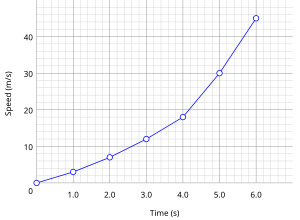
\includegraphics[width=\linewidth]{Pictures/data/data_line_chart.jpg}
            \caption{Graph: Line Plot}
        \end{figure}
    \end{minipage}
\end{table}


\section{Bar Graph \cite{wiki-bar-chart}}\label{graph_bar}
A bar chart or bar graph is a chart or graph that presents categorical data with rectangular bars with heights or lengths proportional to the values that they represent. The bars can be plotted vertically or horizontally. A vertical bar chart is sometimes called a \textbf{column chart}\indexlabel{column chart}.

\vspace{-1cm}

\begin{center}
    \begin{figure}
        \centering
        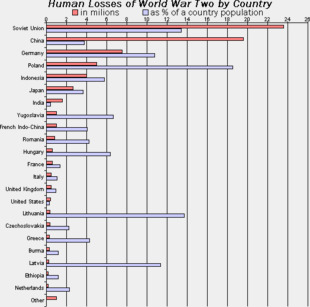
\includegraphics[height=5.6cm]{Pictures/data/data_graph_bar.jpg}
        \caption{Graph: Bar Graph}
    \end{figure}
\end{center}


\section{Histogram \cite{ism-2, wiki-histogram}}\label{histogram}
\subsection{Constructing a Histogram for Discrete Data}
\begin{enumerate}
    \item determine the frequency and relative frequency of each x value
    \item mark possible x values on a horizontal scale
    \item Above each x value, draw a rectangle whose height is the relative frequency (or alternatively, the frequency) of that value
\end{enumerate}

\subsection{Constructing a Histogram for Continuous Data: Equal Class Widths}
\begin{enumerate}
    \item Determine the frequency and relative frequency for each class.
    \item Mark the class boundaries on a horizontal measurement axis.
    \item Above each class interval, draw a rectangle whose height is the corresponding relative frequency (or frequency).
\end{enumerate}

\subsection{Constructing a Histogram for Continuous Data: Unequal Class Widths}
\begin{enumerate}
    \item After determining frequencies and relative frequencies, calculate the height of each rectangle using the formula:
    \begin{equation}
        (rectangle\_height) = (relative\_frequency\_of\_the\_class) / (class\_width)
    \end{equation}
    \item The resulting rectangle heights are usually called \textbf{densities}\indexlabel{densities (histogram)}, and the vertical scale is the density scale. 
    \item This prescription will also work when class widths are equal. 
    \item the area of each rectangle is proportional to the relative frequency of the value
\end{enumerate}

\begin{table}[H]
    \begin{minipage}{0.45\textwidth}
        \centering
        \begin{tabular}{|c|c|}
            \hline
            Bin/Interval & Count/Frequency \\ \hline
            -3.5 to -2.51 & 9 \\ \hline
            -2.5 to -1.51 & 32 \\ \hline
            -1.5 to -0.51 & 109 \\ \hline
            -0.5 to 0.49 & 180 \\ \hline
            0.5 to 1.49 & 132 \\ \hline
            1.5 to 2.49 & 34 \\ \hline
            2.5 to 3.49 & 4 \\ \hline
        \end{tabular}
        \caption{Data: Histogram}
    \end{minipage}
    \hfill
    \begin{minipage}{0.45\textwidth}
        \begin{figure}[H]
            \centering
            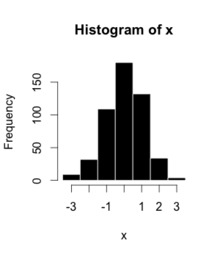
\includegraphics[height=5cm]{Pictures/data/data_histogram.jpg}
            \caption{Graph: Histogram}
        \end{figure}
    \end{minipage}
\end{table}


\section{Stem-and-Leaf Displays \cite{ism-2,wiki-Stem-and-leaf_display}}\label{Stem-and-Leaf Displays}
\begin{enumerate}
    \item Consider a numerical data set x1, .., xn for which each xi consists of at least two digits. 
    \item A quick way to obtain an informative visual representation of the data set is to construct a stem-and-leaf display.
    \item A stem-and-leaf display conveys information about the following aspects of the data:
    \begin{enumerate}
        \item identification of a typical or representative value
        \item extent of spread about the typical value
        \item presence of any gaps in the data
        \item extent of symmetry in the distribution of values
        \item number and location of peaks
        \item presence of any outlying values
    \end{enumerate}
\end{enumerate}
\subsection{Constructing a Stem-and-Leaf Display}
\begin{enumerate}
    \item Select one or more leading digits for the stem values. The trailing digits become the leaves
    \item List possible stem values in a vertical column.
    \item Record the leaf for each observation beside the corresponding stem value
    \item Indicate the units for stems and leaves someplace in the display
\end{enumerate}

\section{Dotplots \cite{wiki-dotplot,ism-2}}\label{dotplots}
\begin{enumerate}
    \item A dotplot is an attractive summary of numerical data when the data set is reasonably small or there are relatively few distinct data values. 
    \item Each observation is represented by a dot above the corresponding location on a horizontal measurement scale. 
    \item When a value occurs more than once, there is a dot for each occurrence, and these dots are stacked vertically
    \item A dotplot gives information about location, spread, extremes, and gaps
\end{enumerate}

\begin{figure}
    \centering
    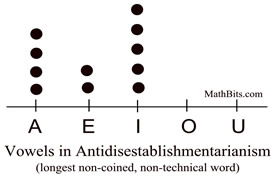
\includegraphics[height=3cm]{Pictures/data/data_dotplot.jpg}
    \caption{Graph: Dotplot}
\end{figure}

\section{Quantile-Quantile Plot \cite{wiki-q-q-plot}}\label{Quantile-Quantile Plot}
A Q–Q plot (quantile–quantile plot) is a probability plot, a graphical method for comparing two probability distributions by plotting their quantiles against each other. A point (x, y) on the plot corresponds to one of the quantiles of the second distribution (y-coordinate) plotted against the same quantile of the first distribution (x-coordinate). This defines a parametric curve where the parameter is the index of the quantile interval.

\begin{table}[H]
    \begin{minipage}{0.45\textwidth}
        \begin{figure}[H]
            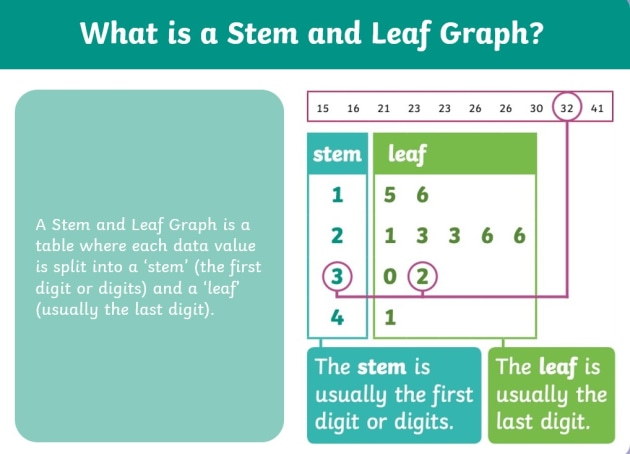
\includegraphics[height=5cm]{Pictures/data/data_stem-and-leaf-plot.jpg}
            \caption{Graph: Stem \& Leaf Plot}
        \end{figure}
    \end{minipage}
    \hfill
    \begin{minipage}{0.45\textwidth}
        \begin{figure}[H]
            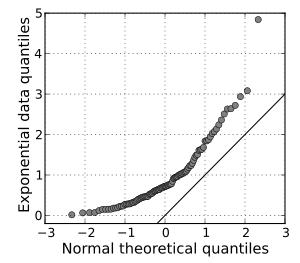
\includegraphics[height=5cm]{Pictures/data/data_q_q_plot.png}
            \caption{Graph: Quantile–Quantile (Q–Q) plot}
        \end{figure}
    \end{minipage}
\end{table}


\section{Box and Whisker plots (aka Box Plot)}\label{Box and Whisker plots (aka Box Plot)}
A box plot or boxplot is a method for demonstrating graphically the locality, spread and skewness groups of numerical data through their quartiles. In addition to the box on a box plot, there can be lines (which are called whiskers) extending from the box indicating variability outside the upper and lower quartiles, thus, the plot is also called the box-and-whisker plot and the box-and-whisker diagram. Outliers that differ significantly from the rest of the dataset may be plotted as individual points beyond the whiskers on the box-plot. Box plots are non-parametric: they display variation in samples of a statistical population without making any assumptions of the underlying statistical distribution (though Tukey's boxplot assumes symmetry for the whiskers and normality for their length). The spacings in each subsection of the box-plot indicate the degree of dispersion (spread) and skewness of the data, which are usually described using the five-number summary. In addition, the box-plot allows one to visually estimate various L-estimators, notably the interquartile range, midhinge, range, mid-range, and trimean. Box plots can be drawn either horizontally or vertically.

\begin{enumerate}
    \item features:
    \begin{enumerate}
        \item center
        \item spread
        \item the extent and nature of any departure from symmetry
        \item identification of “outliers”
    \end{enumerate}
\end{enumerate}

\subsection{Steps to build Box plot}
\begin{enumerate}
    \item Order the n observations from smallest to largest and separate the smallest half from the largest half; the median is included in both halves if n is odd.
    \item Then the lower fourth (1st quartile) is the median of the smallest half and the upper fourth (3rd quartile) is the median of the largest half.
    \item A measure of spread that is resistant to outliers is the fourth spread (aka IQR) fs, given by fs = upper fourth - lower fourth
    \item Any observation farther than 1.5fs from the closest fourth is an outlier
    \item An outlier is extreme if it is more than 3fs from the nearest fourth, and it is mild otherwise.
    \item draw a horizontal measurement scale
    \item place a rectangle above this axis; the left edge of the rectangle is at the lower fourth, and the right edge is at the upper fourth (box width = fs)
    \item Place a vertical line segment or some other symbol inside the rectangle at the location of the median; the position of the median symbol relative to the two edges conveys information about skewness in the middle 50% of the data
    \item draw “whiskers” out from either end of the rectangle to the smallest and largest observations that are not outliers
    \item Each mild outlier is represented by a closed circle and each extreme outlier by an open circle
\end{enumerate}

\begin{figure}[H]
    \centering
    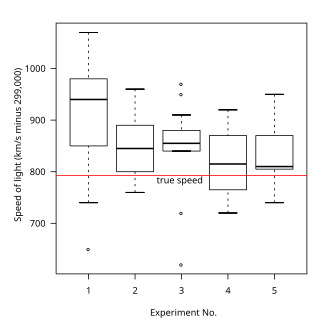
\includegraphics[height=6cm]{Pictures/data/data_box-plot.jpg}
    \caption{Graph: Box Plot}
\end{figure}

































    %%%%%%%%%%         DATA STRUCTs         %%%%%%%%%%

\chapter{Data Structures \cite{gfg-data-structures}}\label{Data Structures}

\section{What is Data Structure? \cite{gfg-introduction-to-data-structures}}
\begin{itemize}
    \item A data structure is a particular way of organising data in a computer so that it can be used effectively. 
    
    \item The idea is to reduce the space and time complexities of different tasks. 

    \item A data structure is a storage that is used to store and organize data. It is a way of arranging data on a computer so that it can be accessed and updated efficiently.

    \item Data structures are the fundamental building blocks of computer programming. 
    
    \item They define how data is organized, stored, and manipulated within a program. 
    
    \item Understanding data structures is very important for developing efficient and effective algorithms.
\end{itemize}


\section{Types of Data Structure \cite{gfg-introduction-to-data-structures}}

\begin{figure}[h]
    \centering
    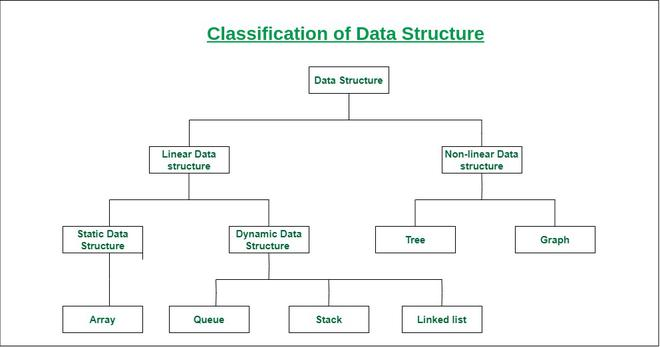
\includegraphics[width=0.5\linewidth,height=6cm,keepaspectratio]{Pictures/ds-algo/ClassificationofDataStructures.jpg}
    \caption{Types of Data Structure}
\end{figure}

\subsection{Linear Data Structure \cite{gfg-data-structures}}
\begin{itemize}
    \item Data structure in which data elements are arranged sequentially or linearly, where each element is attached to its previous and next adjacent elements, is called a linear data structure.
    
    \item \textbf{Example}: Array, Stack, Queue, Linked List, etc.
\end{itemize}

\subsection{Static Data Structure \cite{gfg-data-structures}}
\begin{itemize}
    \item Static data structure has a fixed memory size. It is easier to access the elements in a static data structure. 

    \item \textbf{Example}: array.
\end{itemize}

\subsection{Dynamic Data Structure \cite{gfg-data-structures}}
\begin{itemize}
    \item In dynamic data structure, the size is not fixed. It can be randomly updated during the runtime which may be considered efficient concerning the memory (space) complexity of the code.

    \item \textbf{Example}: Queue, Stack, etc.
\end{itemize}

\subsection{Non-Linear Data Structure \cite{gfg-data-structures}}
\begin{itemize}
    \item Data structures where data elements are not placed sequentially or linearly are called non-linear data structures. In a non-linear data structure, we can’t traverse all the elements in a single run only.
    
    \item \textbf{Example}: Trees and Graphs.
\end{itemize}

\section{Array \cite{gfg-array-data-structure-guide}}\label{array}

\begin{table}[h]
    \begin{minipage}{0.35\linewidth}
        \begin{figure}[H]
            \centering
            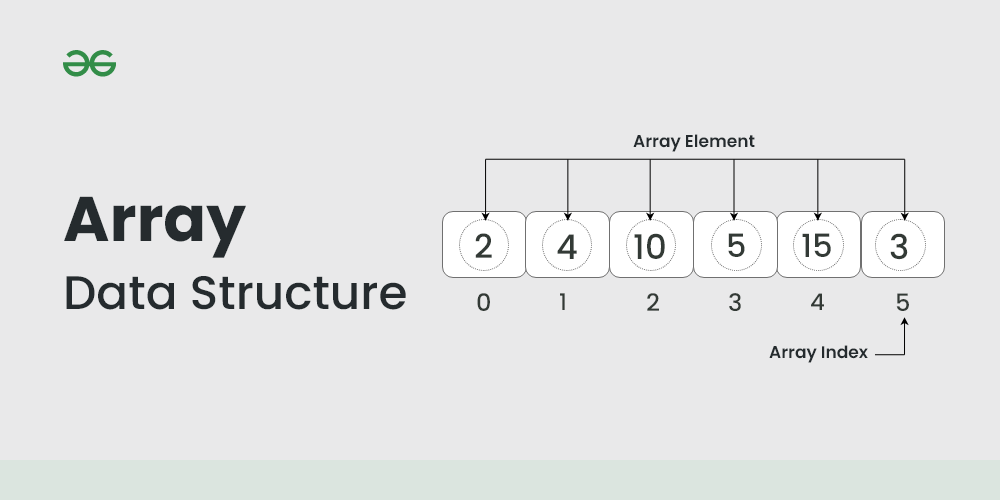
\includegraphics[width=\linewidth,height=5cm,keepaspectratio]{Pictures/ds-algo/Array-data-structure.png}
            \caption{Data Structure: Array}
        \end{figure}
    \end{minipage}
    \hfill
    \begin{minipage}{0.65\linewidth}
        \begin{itemize}
            \item An array data structure is a fundamental concept in computer science that stores a collection of elements in a contiguous block of memory.

            \item It allows for efficient access to elements using indices and is widely used in programming for organizing and manipulating data.

            \item Each item in an array is indexed starting with $\mathbf{0}$. 
            
            \item Each element in an array is accessed through its index.
        \end{itemize}
    \end{minipage}
\end{table}

\noindent \textbf{Types of Array}
\begin{enumerate}
    \item \textbf{One-dimensional arrays}: These arrays store a single row of elements.
    \item \textbf{Multidimensional arrays}: These arrays store multiple rows of elements.
\end{enumerate}

\subsection{Array Operations}
\begin{itemize}
    \item \fullref{Linear Search Algorithm}
    \item \fullref{Binary Search Algorithm}
    \item \fullref{Ternary Search}
    \item \fullref{Exponential Search}
\end{itemize}














































%%%%%%%%%%         ALGOs            %%%%%%%%%%

\chapter{Algorithms: Search}

\section{Linear Search Algorithm \cite{gfg-linear-search}}\label{Linear Search Algorithm}

\begin{table}[h]
    \begin{minipage}[t]{0.5\linewidth}
        \begin{figure}[H]
            \centering
            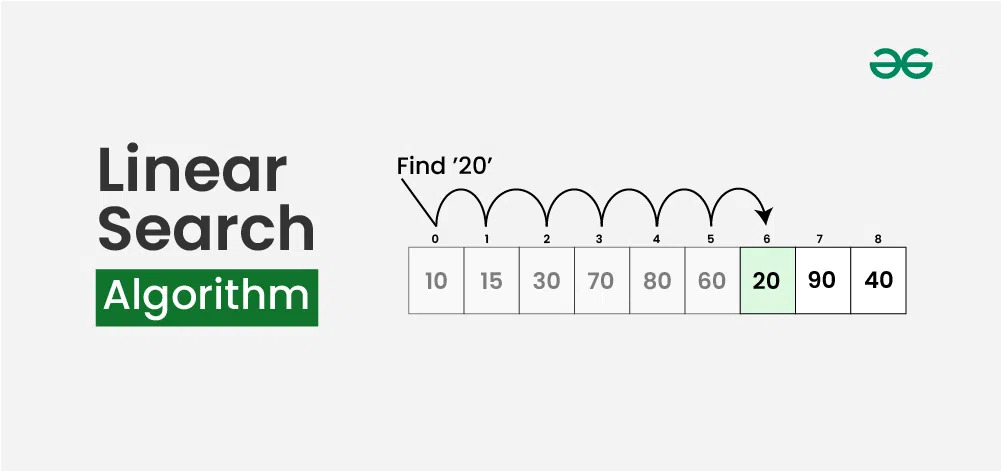
\includegraphics[width=\linewidth,height=6cm,keepaspectratio]{Pictures/ds-algo/Linear-Search-algorithm.jpg}
            \caption{Linear Search Algorithm}
        \end{figure}
    \end{minipage}
    \hfill
    \begin{minipage}[t]{0.35\linewidth}
        \begin{table}[H]
            \begin{tabular}{l l l}
                \multicolumn{3}{c}{\textbf{Time Complexity}} \\
                 Best Case & $O(1)$ & first index \\
                 Average Case & $O(N)$ &  \\
                 Worst Case & $O(N)$ & last index \\
                 \multicolumn{3}{c}{\textbf{Space Complexity}}\\
                 Auxiliary Space & $O(1)$ & iterator \\
            \end{tabular}
        \end{table}
    \end{minipage}
\end{table}

\textbf{Steps}:
\begin{enumerate}
    \item \textbf{Start}: Begin at the first element of the collection of elements.
    \item \textbf{Compare}: Compare the current element with the desired element.
    \item \textbf{Found}: If the current element is equal to the desired element, return true or index to the current element.
    \item \textbf{Move}: Otherwise, move to the next element in the collection.
    \item \textbf{Repeat}: Repeat steps 2-4 until we have reached the end of collection.
    \item \textbf{Not found}: If the end of the collection is reached without finding the desired element, return that the desired element is not in the array.
\end{enumerate}

\begin{table}[h]
    \begin{minipage}[t]{0.48\linewidth}
        \textbf{Advantages}:
        \begin{itemize}
            \item Linear search can be used irrespective of whether the array is sorted or not. 
            \item It can be used on arrays of any data type.
            \item Does not require any additional memory.
            \item It is a well-suited algorithm for small datasets.
        \end{itemize}
    \end{minipage}
    \hfill
    \begin{minipage}[t]{0.48\linewidth}
        \textbf{Disadvantages}:
        \begin{itemize}
            \item Linear search has a time complexity of $O(N)$, which in turn makes it \textbf{SLOW} for large datasets.
            \item \textbf{NOT} suitable for large arrays.
        \end{itemize}
    \end{minipage}
\end{table}

\begin{lstlisting}[language=Python, caption=Linear Search Algorithm - Python]
def search(arr: list, N: int, x: object) -> int:
    for i in range(0, N):
        if (arr[i] == x):
            return i
    return -1
\end{lstlisting}

\section{Binary Search Algorithm \cite{gfg-binary-search}} \label{Binary Search Algorithm}

\begin{table}[H]
    \begin{minipage}[t]{0.45\linewidth}
        \begin{figure}[H]
            \centering
            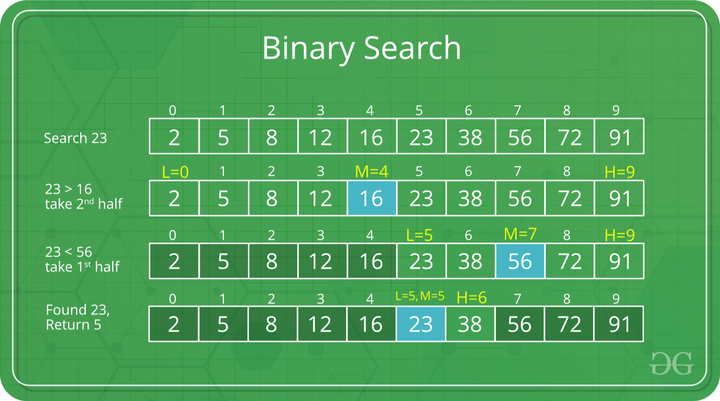
\includegraphics[width=\linewidth,height=6cm,keepaspectratio]{Pictures/ds-algo/BinarySearch.png}
            \caption{Binary Search Algorithm}
        \end{figure}
    \end{minipage}
    \hfill
    \begin{minipage}[t]{0.55\linewidth}
        \begin{table}[H]
            \begin{tabular}{l l l}
                \multicolumn{3}{c}{\textbf{Time Complexity}} \\
                 Best Case & $O(1)$ & \\
                 Average Case & $O(\log(N))$ &  \\
                 Worst Case & $O(\log(N))$ &  \\
                 \multicolumn{3}{c}{\textbf{Space Complexity}}\\
                 Auxiliary Space & $O(1)$ & \\
                 Auxiliary Space & $O(\log(N))$ & recursive call stack \\
            \end{tabular}
        \end{table}
    \end{minipage}
\end{table}


\textbf{Steps}:
\begin{enumerate}
    \item Divide the search space into two halves by finding the middle index “mid”.
    \item Compare the middle element of the search space with the key.
    \item If the key is found at middle element, the process is terminated.
    \item If the key is not found at middle element, choose which half will be used as the next search space.
    \begin{enumerate}
        \item If the key is smaller than the middle element, then the left side is used for next search.
        \item If the key is larger than the middle element, then the right side is used for next search.
    \end{enumerate}
    \item This process is continued until the key is found or the total search space is exhausted.
\end{enumerate}

\begin{table}[h]
    \begin{minipage}[t]{0.48\linewidth}
        \textbf{Advantages}:
        \begin{itemize}
            \item Binary search is faster than linear search, especially for large arrays.
            \item More efficient than other searching algorithms with a similar time complexity, such as interpolation search or exponential search.
            \item Binary search is well-suited for searching large datasets that are stored in external memory, such as on a hard drive or in the cloud.
        \end{itemize}
    \end{minipage}
    \hfill
    \begin{minipage}[t]{0.48\linewidth}
        \textbf{Disadvantages}:
        \begin{itemize}
            \item The array should be \textbf{sorted}.
            \item Binary search requires that the data structure being searched be stored in contiguous memory locations. 
            \item Binary search requires that the elements of the array be comparable, meaning that they must be able to be ordered.
        \end{itemize}
    \end{minipage}
\end{table}

\begin{lstlisting}[language=Python, caption=Binary Search (iterative) - Python]
def binarySearch(arr: list, low: int, high: int, x: object) -> int:
    while low <= high:
        mid = low + (high - low) // 2

        # Check if x is present at mid
        if arr[mid] == x: return mid

        # If x is greater, ignore left half
        elif arr[mid] < x: low = mid + 1

        # If x is smaller, ignore right half
        else: high = mid - 1

    # If we reach here, then the element was not present
    return -1
\end{lstlisting}

\begin{lstlisting}[language=Python, caption=Binary Search (recursive) - Python]
def binarySearch(arr: list, low: int, high: int, x: object) -> int:
    # Check base case
    if high >= low:
        mid = low + (high - low) // 2
        
        # If element is present at the middle itself
        if arr[mid] == x: return mid
            
        # If element is smaller than mid, then it
        # can only be present in left subarray
        elif arr[mid] > x: 
            return binarySearch(arr, low, mid-1, x)

        # Else the element can only be 
        # present in right subarray
        else: return binarySearch(arr, mid + 1, high, x)

    # Element is not present in the array
    else: return -1
\end{lstlisting}

\section{Ternary Search \cite{gfg-ternary-search}}\label{Ternary Search}
\begin{table}[h]
    \begin{minipage}{0.5\linewidth}
        \begin{figure}[H]
            \centering
            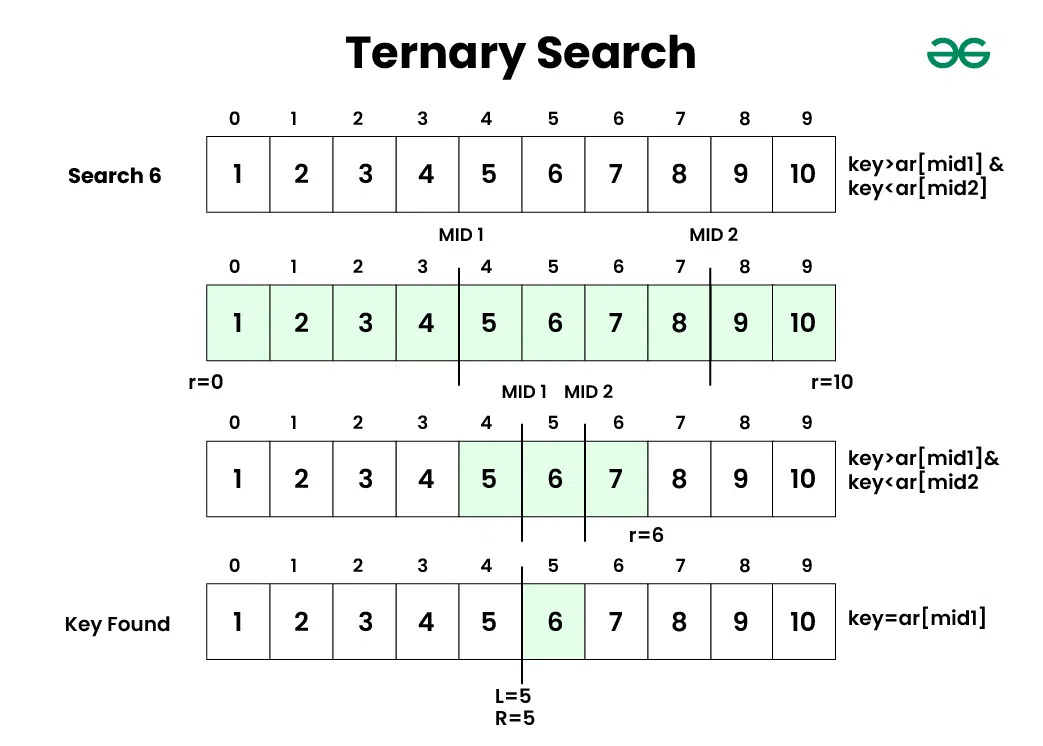
\includegraphics[width=\linewidth, height=10cm, keepaspectratio]{Pictures/ds-algo/Ternary-Search.jpg}
            \caption{Ternary Search}
        \end{figure}
    \end{minipage}
    \hfill
    \begin{minipage}{0.47\linewidth}
        \begin{table}[H]
            \begin{tabular}{l l l}
                \multicolumn{3}{c}{\textbf{Time Complexity}} \\
                 Recursive & $O(2*\log_3(N))$ & \\
                 Iterative & $O(\log_3(N))$ & \\
                 \multicolumn{3}{c}{\textbf{Space Complexity}}\\
                 Auxiliary Space & $O(2*\log_3(N))$ & Recursive \\
                 Auxiliary Space & $O(1)$ & Iterative \\
            \end{tabular}
        \end{table}
    \end{minipage}
\end{table}

\vspace{0.2cm}
\textbf{Steps}:
\begin{enumerate}
    \item \textbf{Initialization}: Set two pointers, \textbf{left} and \textbf{right}, initially pointing to the first and last elements of our search space.

    \item \textbf{Divide the search space}:
    \begin{enumerate}
        \item Calculate two midpoints, mid1 and mid2, dividing the current search space into three roughly equal parts:
        \item[] $mid1 = left + (right - left) / 3$
        \item[] $mid2 = right - (right - left) / 3$
        \item The array is now effectively divided into $[left, mid1]$, $(mid1, mid2)$, and $[mid2, right]$.
    \end{enumerate}

    \item \textbf{Comparison with Target}:
    \begin{enumerate}
        \item If the \textbf{target} is equal to the element at \textbf{mid1} or \textbf{mid2}, the search is successful, and the index is returned.

        \item If the target is less than the element at mid1, update the right pointer to $mid1 - 1$.

        \item If the target is greater than the element at mid2, update the left pointer to $mid2 + 1$.

        \item If the target is between the elements at mid1 and mid2, update the left pointer to $mid1 + 1$ and the right pointer to $mid2 - 1$.
    \end{enumerate}

    \item \textbf{Repeat or Conclude}:
    \begin{enumerate}
        \item Repeat the process with the reduced search space until the target is found or the search space becomes empty.

        \item If the search space is empty and the target is not found, return a value indicating that the target is not present in the array.
    \end{enumerate}
\end{enumerate}

\begin{table}[h]
    \begin{minipage}[t]{0.48\linewidth}
        \textbf{Advantages}:
        \begin{itemize}
            \item Ternary search can find maxima/minima for unimodal functions, where binary search is not applicable.
            
            \item Ternary Search has a time complexity of $O(2 * \log_3(N))$, which is more efficient than linear search and comparable to binary search.

            \item Fits well with optimization problems.
        \end{itemize}
    \end{minipage}
    \hfill
    \begin{minipage}[t]{0.48\linewidth}
        \textbf{Disadvantages}:
        \begin{itemize}
            \item Ternary Search is only applicable to ordered lists or arrays, and cannot be used on unordered or non-linear data sets.

            \item Ternary Search takes more time to find maxima/ minima of monotonic functions as compared to Binary Search.
        \end{itemize}
    \end{minipage}
\end{table}

\begin{lstlisting}[language=Python, caption=Ternary Search (recursive) - Python]
def ternarySearch(l: int, r: int, key: int, ar: list) -> int:
    if (r >= l):
        # Find the mid1 and mid2
        mid1 = l + (r - l) //3
        mid2 = r - (r - l) //3

        # Check if key is present at any mid
        if (ar[mid1] == key):  return mid1
        
        if (ar[mid2] == key): return mid2
        
        # Since key is not present at mid,
        # check in which region it is present
        # then repeat the Search operation
        # in that region
        if (key < ar[mid1]): 
            # The key lies in between l and mid1
            return ternarySearch(l, mid1 - 1, key, ar)
        
        elif (key > ar[mid2]): 
            # The key lies in between mid2 and r
            return ternarySearch(mid2 + 1, r, key, ar)
        
        else: 
            # The key lies in between mid1 and mid2
            return ternarySearch(mid1 + 1, mid2 - 1, key, ar)
        
    # Key not found
    return -1
\end{lstlisting}
\begin{lstlisting}[language=Python, caption=Ternary Search (iterative) - Python]
def ternarySearch(l: int, r: int, key: int, ar: list) -> int:
    while r >= l:
        # Find mid1 and mid2
        mid1 = l + (r-l) // 3
        mid2 = r - (r-l) // 3

        # Check if key is at any mid
        if key == ar[mid1]: return mid1
        if key == ar[mid2]: return mid2

        # Since key is not present at mid, 
        # Check in which region it is present
        # Then repeat the search operation in that region
        if key < ar[mid1]:
            # key lies between l and mid1
            r = mid1 - 1
        elif key > ar[mid2]:
            # key lies between mid2 and r
            l = mid2 + 1
        else:
            # key lies between mid1 and mid2
            l = mid1 + 1
            r = mid2 - 1

    # key not found
    return -1
\end{lstlisting}


\section{Exponential Search \cite{gfg-exponential-search}}\label{Exponential Search}

\begin{table}[h]
    \begin{tabular}{l l l}
         \textbf{Time Complexity} & $O(\log(N))$ &  \\
         \multicolumn{3}{c}{\textbf{Space Complexity}}\\
         Auxiliary Space & $O(1)$ & iterative \\
         Auxiliary Space & $O(\log(N))$ & recursive \\
    \end{tabular}
\end{table}

\textbf{Steps}:
\begin{enumerate}
    \item Find range where element is present
    \item Do \fullref{Binary Search Algorithm} in above found range
\end{enumerate}

\begin{lstlisting}[language=Python, caption=Exponential Search - Python]
# Returns the position of first occurrence of x in array
def exponentialSearch(arr: list, n: int, x: object) -> int:
    # IF x is present at first 
    # location itself
    if arr[0] == x: return 0
         
    # Find range for binary search 
    # j by repeated doubling
    i = 1
    while i < n and arr[i] <= x: i = i * 2
     
    # Call binary search for the found range
    return binarySearch(arr, i // 2, min(i, n-1), x)
\end{lstlisting}

























\chapter{Algorithms: Sort}

\section{Types of sortings \cite{gfg-sorting-algorithms}}
\begin{enumerate}
    \item \textbf{In-place Sorting}\indexlabel{In-place Sorting}: An in-place sorting algorithm uses constant space for producing the output (modifies the given array only).\\
    It sorts the list only by modifying the order of the elements within the list.\\
    \textbf{Examples}: Selection Sort, Bubble Sort Insertion Sort and Heap Sort.

    \item \textbf{Internal Sorting}\indexlabel{Internal Sorting}: Internal Sorting is when all the data is placed in the main memory or internal memory.\\
    In internal sorting, the problem cannot take input beyond (memeory) size.\\
    \textbf{Example}: heap sort, bubble sort, selection sort, quick sort, shell sort, insertion sort.

    \item \textbf{External Sorting}\indexlabel{External Sorting}: External Sorting is when all the data that needs to be sorted cannot be placed in memory at a time, the sorting is called external sorting.\\
    External Sorting is used for the \textit{massive amount of data}.\\
    \textbf{Examples}: Merge sort, Tag sort, Polyphase sort, Four tape sort, External radix sort, etc.

    \item \textbf{Stable sorting}\indexlabel{Stable sorting}: When two same data appear in the same order in sorted data without changing their position is called stable sort. \\
    \textbf{Examples}: Merge Sort, Insertion Sort, Bubble Sort.

    \item \textbf{Unstable sorting}\indexlabel{Unstable sorting}: When two same data appear in the different order in sorted data it is called unstable sort.\\
    \textbf{Examples}: Quick Sort, Heap Sort, Shell Sort.

\end{enumerate}

\vspace{4cm}
\url{https://www.geeksforgeeks.org/sorting-algorithms/}





\chapter{Dynamic Programming (DP) \cite{gfg-dynamic-programming}}

\textbf{Dynamic Programming (DP)} is a method used in mathematics and computer science to solve complex problems by breaking them down into simpler subproblems. By solving each subproblem only once and storing the results, it avoids redundant computations, leading to more efficient solutions for a wide range of problems.

\section{How Does Dynamic Programming (DP) Work?}

\begin{itemize}
    \item \textbf{Identify Subproblems}: Divide the main problem into smaller, independent subproblems.
    \item \textbf{Store Solutions}: Solve each subproblem and store the solution in a table or array.
    \item \textbf{Build Up Solutions}: Use the stored solutions to build up the solution to the main problem.
    \item \textbf{Avoid Redundancy}: By storing solutions, DP ensures that each subproblem is solved only once, reducing computation time.
\end{itemize}

\begin{table}[H]
    \begin{minipage}{0.45\linewidth}
        \begin{figure}[H]
            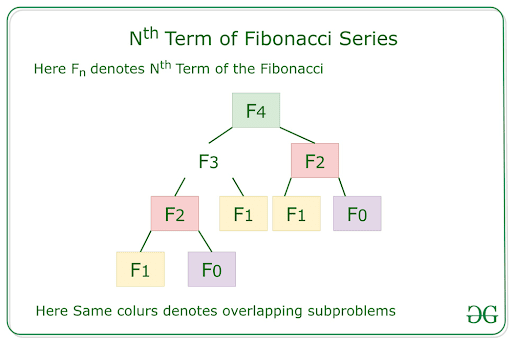
\includegraphics[height=5cm]{Pictures/ds-algo/nthfibonacciseriesdynamicprogramming.png}
        \end{figure}
    \end{minipage}
    \hfill
    \begin{minipage}{0.52\linewidth}
        \begin{itemize}
            \item \textbf{Subproblems}: $F(0)$, $F(1)$, $F(2)$, $F(3)$, ...
            \item \textbf{Store Solutions}: Create a table to store the values of $F(n)$ as they are calculated.
            \item \textbf{Build Up Solutions}: For $F(n)$, look up $F(n-1)$ and $F(n-2)$ in the table and add them.
            \item \textbf{Avoid Redundancy}: The table ensures that each subproblem (e.g., $F(2)$) is solved only once.
        \end{itemize}        
    \end{minipage}
\end{table}



\section{When to Use Dynamic Programming (DP)?}

\begin{enumerate}
    \item \textbf{Optimal Substructure}:\\
    Optimal substructure means that we combine the optimal results of subproblems to achieve the optimal result of the bigger problem.
    \item \textbf{Overlapping Subproblems}:\\
    The same subproblems are solved repeatedly in different parts of the problem.
\end{enumerate}

\section{Approaches of Dynamic Programming (DP)}

\subsection{Top-Down Approach (Memoization)}
In the top-down approach, also known as \textbf{memoization}, we start with the final solution and recursively break it down into smaller subproblems. To avoid redundant calculations, we store the results of solved subproblems in a memoization table. Suitable when the number of subproblems is large and many of them are reused.

\subsection{Bottom-Up Approach (Tabulation)}
In the bottom-up approach, also known as \textbf{tabulation}, we start with the smallest subproblems and gradually build up to the final solution. We store the results of solved subproblems in a table to avoid redundant calculations. Suitable when the number of subproblems is small and the optimal solution can be directly computed from the solutions to smaller subproblems.



































































































    
    \chapter{Data for ML}

\begin{itemize}
    \item The table of examples ${x_1, ..., x_N}$ is often concatenated, and written as $X \in R^{N \times D}$
    \item We will discuss finding good representations in two ways:
    \begin{itemize}
        \item Finding lower-dimensional approximations of the original feature vector
        \item Using nonlinear higher-dimensional combinations of the original feature vector
    \end{itemize}
\end{itemize}


\section{Types of Datasets}\label{Types of Datasets}

\subsection{Training Data/ Train Set}\label{data_train}
\begin{itemize}
    \item Actual data that is used to train the model
\end{itemize}

\subsection{Testing Data/ Test Set}\label{data_test}
\begin{itemize}
    \item Data used to test accuracy of model
    \item Maybe or may not be subset of train set
    \item Unseen data for model
\end{itemize}

\subsection{Validation (val) Set/ Development (dev) Set}\label{data_val_dev}
\begin{itemize}
    \item Data used for cross-validation
    \item Subset of train set
    \item Unseen data for model (atleast not directly)
\end{itemize}

\vspace{0.2cm}


\textbf{Note:}
\begin{itemize}
    \item Sometimes test set and val set are used interchangeably
\end{itemize}

\section{Distribution Shift \cite{dnn-1,mit-imbalance-outliers-shift}}

Distribution shift is a challenging problem that occurs when the joint distribution of inputs and outputs differs between training and test stages.

\begin{table}[H]
    \begin{minipage}{0.45\textwidth}
        \begin{figure}[H]
            \centering
            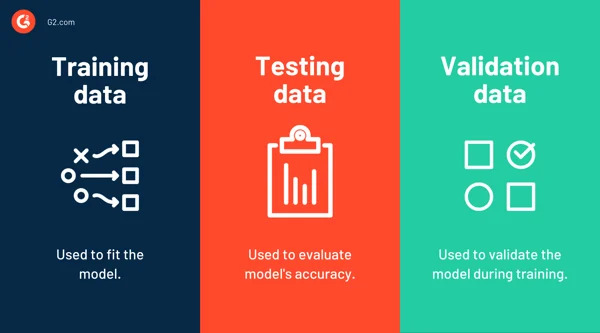
\includegraphics[width=7.5cm,height=4cm]{Pictures/ml-data/ml-datasets-type.jpg}
            \caption{Datasets: Types}
        \end{figure}
    \end{minipage}
    \hfill
    \begin{minipage}{0.45\textwidth}
        \begin{figure}[H]
            \centering
            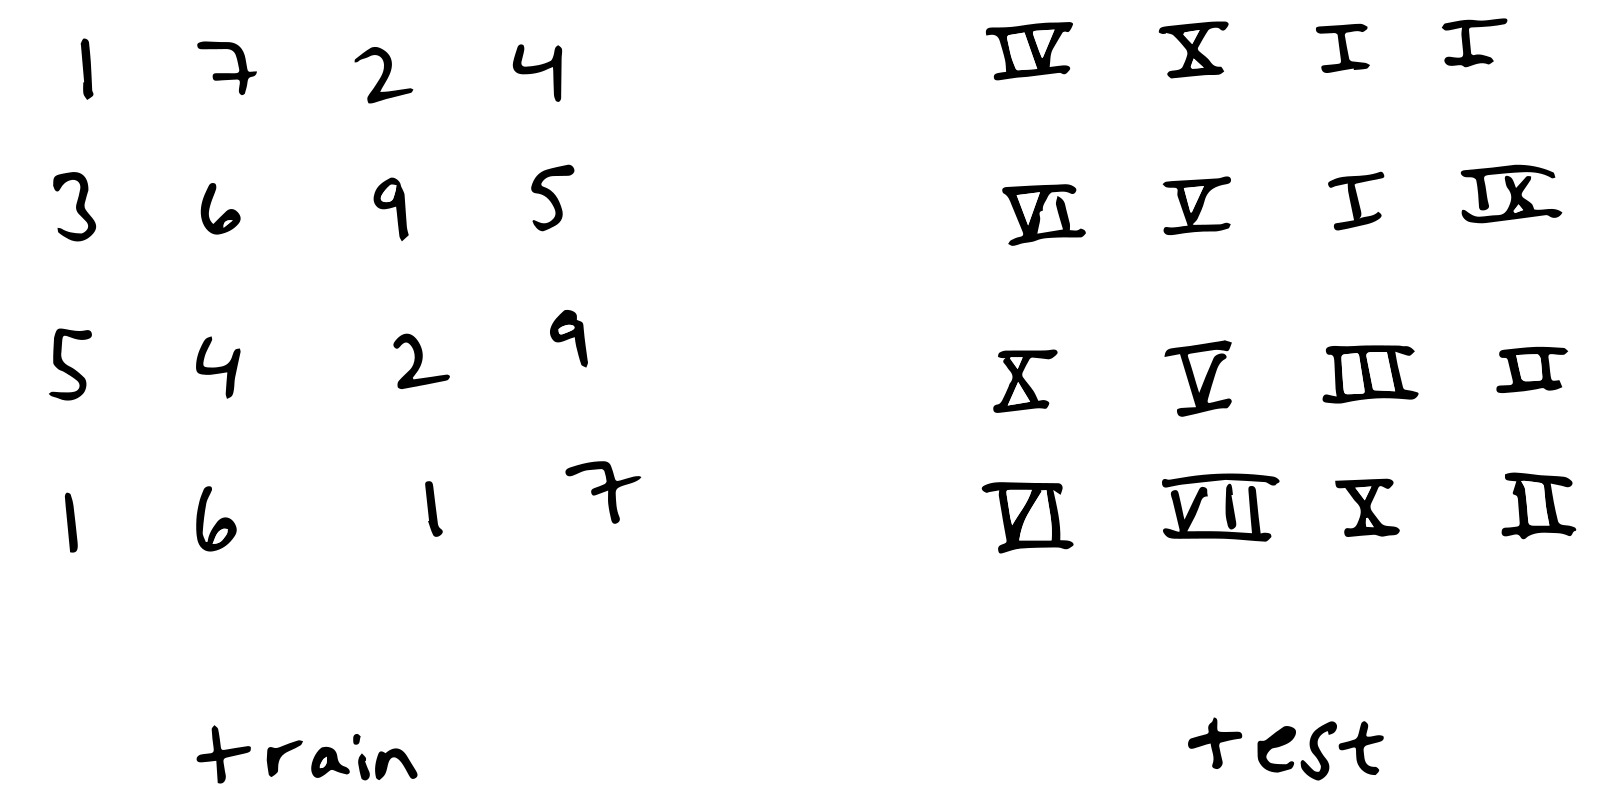
\includegraphics[width=7.5cm,height=4cm]{Pictures/ml-data/ml-data-distribution-shift.jpg}
            \caption{Distribution Shift}
        \end{figure}
    \end{minipage}
\end{table}

\subsection{Covariate shift / data shift}\label{data_shift}
Covariate shift occurs when $p(x)$ changes between train and test, but $p(y|x)$ does not. In other words, the distribution of inputs changes between train and test, but the relationship between inputs and outputs does not change.

\vspace{0.2cm}
\textbf{Examples of covariate shift:}
\begin{itemize}
    \item Self-driving car trained on the sunny streets of San Francisco and deployed in the snowy streets of Boston
    \item Speech recognition model trained on native English speakers and then deployed for all English speakers
    \item Diabetes prediction model trained on hospital data from Boston and deployed in India
\end{itemize}

\begin{table}[H]
    \begin{minipage}{0.45\textwidth}
        \begin{figure}[H]
            \centering
            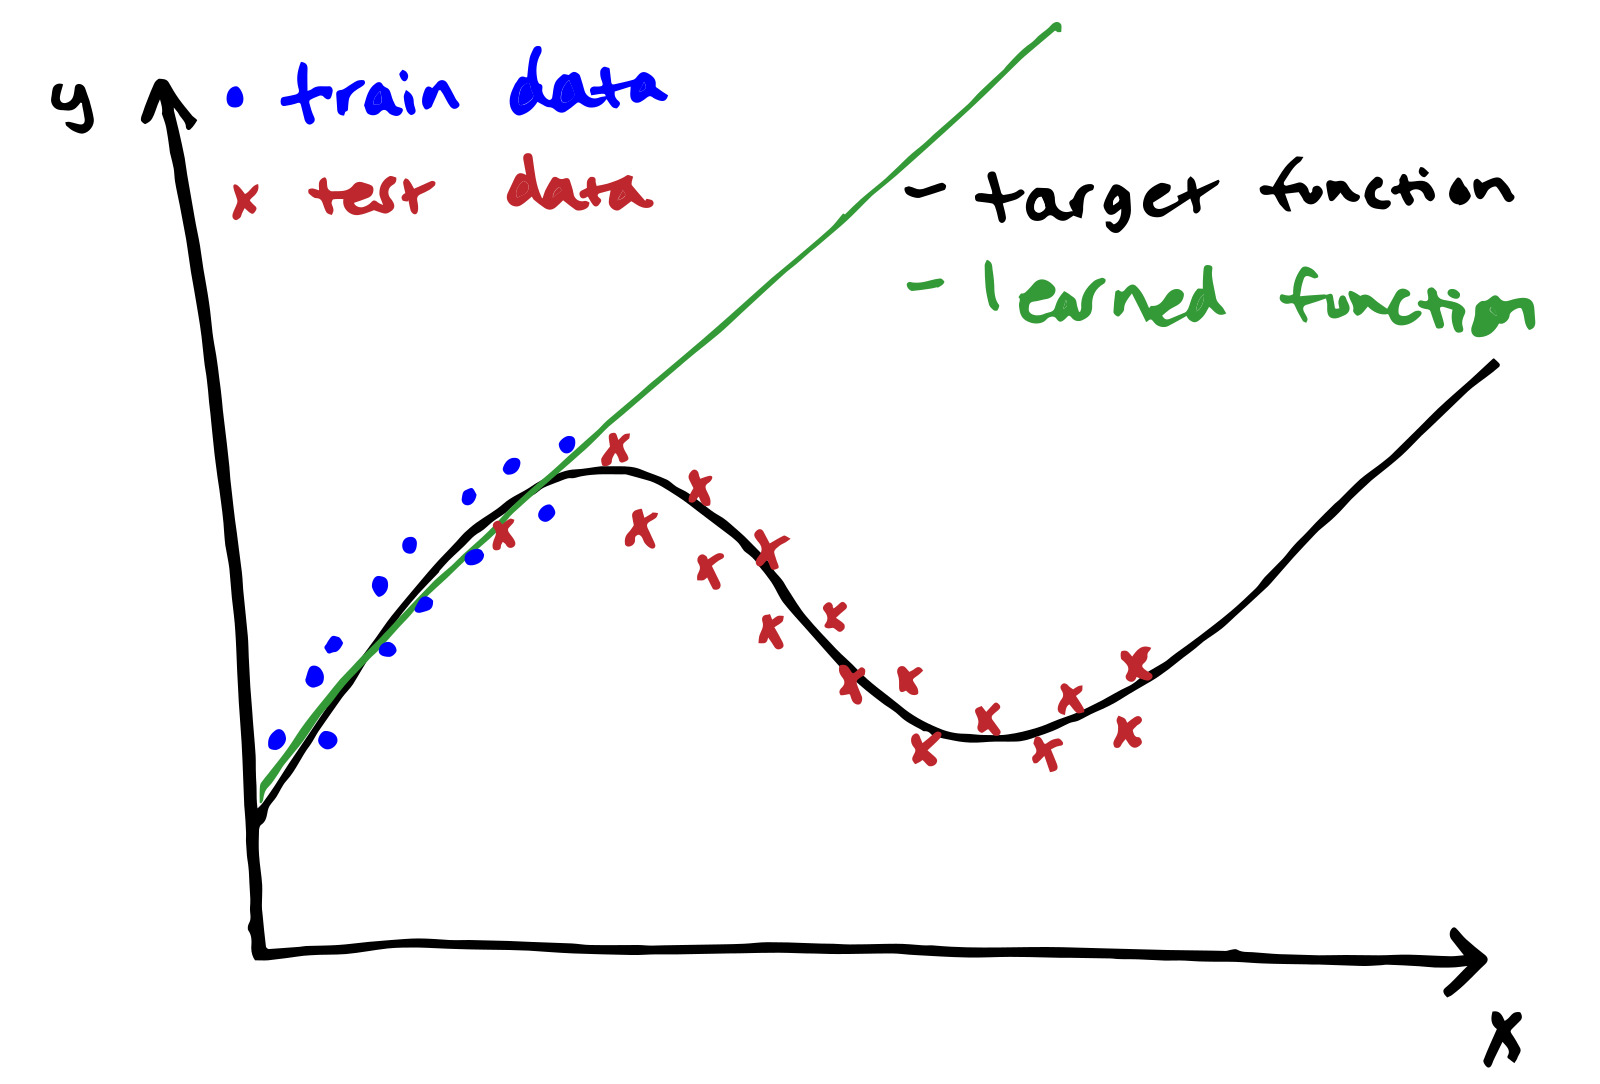
\includegraphics[width=7.5cm,height=4cm]{Pictures/ml-data/ml-data-covariate-shift.jpg}
            \caption{Distribution Shift: Covariate Shift/ Data Shift}
        \end{figure}
    \end{minipage}
    \hfill
    \begin{minipage}{0.45\textwidth}
        \begin{figure}[H]
            \centering
            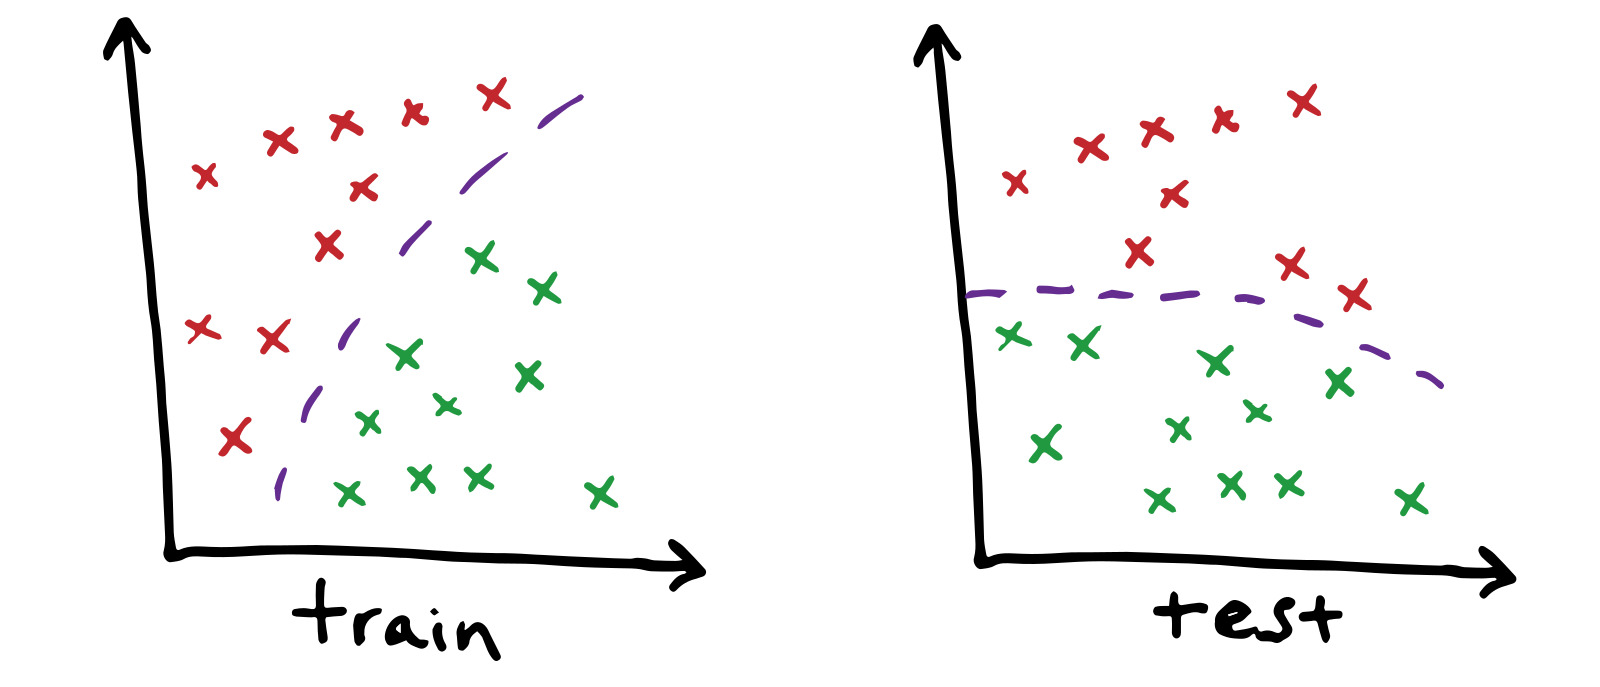
\includegraphics[width=7.5cm,height=4cm]{Pictures/ml-data/ml-data-concept-shift.jpg}
            \caption{Distribution Shift: Concept Shift}
        \end{figure}
    \end{minipage}
\end{table}

\subsection{Concept shift}\label{concept_shift}
Concept shift occurs when $p(y|x)$ changes between train and test, but $p(x)$ does not. In other words, the input distribution does not change, but the relationship between inputs and outputs does. This can be one of the most difficult types of distribution shift to detect and correct.

\vspace{0.2cm}
\textbf{Examples:}
\begin{itemize}
    \item Predicting a stock price based on company fundamentals, trained on data from 1975 and deployed in 2023.
    \item Making purchase recommendations based on web browsing behavior, trained on pre-pandemic data and deployed in March 2020.
\end{itemize}

\subsubsection{Prior probability shift / label shift}\label{label_shift}
Prior probability shift appears only in $y \to x$ problems (when we believe $y$ causes $x$). It occurs when $p(y)$ changes between train and test, but $p(x|y)$ does not. You can think of it as the converse of covariate shift.

\vspace{0.2cm}
\textbf{Examples:}
\begin{itemize}
    \item If the model is trained on a balanced dataset of 50\% spam and 50\% non-spam emails, and then it’s deployed in a real-world setting where 90\% of emails are spam, that is an example of prior probability shift.
\end{itemize}

\section{Covariate Shift (Data Shift) VS Concept Shift VS Prior Probability Shift (Label Shift) \cite{chatgpt}}


\begin{longtable}{|m{3.5cm}|m{4cm}|m{4cm}|m{4cm}|}
    \caption{Covariate Shift (Data Shift) VS Concept Shift VS Prior Probability Shift (Label Shift)} \\ \hline
    
    \textbf{Aspect} & \textbf{Covariate Shift (Data Shift)} & \textbf{Concept Shift} & \textbf{Prior Probability Shift (Label Shift)} \\ \hline
    \endfirsthead
    
    \textbf{Aspect} & \textbf{Covariate Shift (Data Shift)} & \textbf{Concept Shift} & \textbf{Prior Probability Shift (Label Shift)} \\ \hline
    \endhead
    
    \hline\endfoot
    
    \hline\endlastfoot
    
    \textbf{Definition} & Change in the distribution of the input data (features) between training and test sets. & Change in the conditional distribution of the output given the input. & Change in the distribution of the output labels between training and test sets. \\ \hline
    
    \textbf{Cause} & Different data sources, sampling methods, or temporal changes affecting features. & Changes in the underlying relationship between features and labels, often due to evolving contexts or environments. & Variations in the frequency or proportion of different labels in the dataset over time. \\ \hline

    \textbf{Effect} & Model performance degradation due to misaligned feature distributions. & Model predictions become inaccurate because the learned relationships are no longer valid. & Bias in predicted label distribution if not accounted for, leading to misclassification. \\ \hline

    \textbf{Detection} & Comparing feature distributions (e.g., using statistical tests like KS test, histograms). & Analyzing the performance metrics over time or checking for changes in decision boundaries. & Comparing label distributions (e.g., using chi-square tests) or through domain knowledge. \\ \hline

    \textbf{Adjustment Techniques} & Reweighting samples, domain adaptation methods, or using robust models. & Regular retraining with updated data, transfer learning, or domain adaptation techniques. & Adjusting model outputs using methods like importance weighting, resampling, or calibration. \\ \hline

    \textbf{Example} & A retail model trained on summer sales data might perform poorly in winter due to changes in purchasing behavior. & A spam detection model might become less effective if spammers change tactics and the nature of spam emails evolves. & A medical diagnosis model might require adjustment if the prevalence of certain diseases changes in the population. \\ \hline

    \textbf{Relevance in Real-world Applications} & High when dealing with non-stationary environments or merging datasets from different sources. & High in dynamic environments where the relationship between input features and output labels can evolve. & High in situations with shifting class distributions, like seasonal changes or demographic shifts. \\ \hline

\end{longtable}



















    \chapter{Data For ML: Text Data}

\section{Terminologies \cite{nlp-1, chatgpt, ir-1}}
\begin{table}[h!]
    \centering
    \begin{tabular}{| m{2cm} | m{6cm} | m{6cm} |}
        \hline
        \textbf{Term} & \textbf{Definition} & \textbf{Example} \\
        \hline
        \textbf{(Document) Collections} aka \textbf{Corpus} & \vspace{0.2cm}\begin{enumerate}
            \item A group of documents or texts gathered together, often around a specific theme, topic, or source. 
            
            \item Collections can be subsets within a larger corpus.

            \item group of documents over which we perform retrieval \cite{ir-1}
        \end{enumerate} & A collection of scientific articles on climate change, or a collection of user reviews from a specific website. \\
        \hline
        
        \textbf{Documents} & \vspace{0.3cm}\begin{enumerate}
            \item Individual pieces of text within a corpus or a collection. They are the smallest unit of analysis and can vary in length and format.
            
            \item whatever units we have decided to build a retrieval system over. \cite{ir-1}
        \end{enumerate} & A single news article, a research paper, a blog post, or a book chapter. \\
        \hline
        
    \end{tabular}
\end{table}

\section{Herdan’s Law ( $|V| = kN^{\beta}$ ) \cite{nlp-1}} \label{Herdan’s Law}

\[
    |V| = kN^{\beta} \hfill (0 < \beta < 1 \text{ and } k > 0)
\]

\begin{enumerate}
    \item The larger the corpora we look at, the more word types we find.
    \item value of $\beta$ depends on the corpus size and the genre
\end{enumerate}

\section{Datasheet/ Data statement}\label{Datasheet/ Data statement}

A datasheet specifies properties of a dataset like:
\begin{table}[h]
    \centering
    \begin{tabular}{|m{3.5cm}|m{11.5cm}|}
        \hline
        
        \textbf{Motivation} & Why was the corpus collected, by whom, and who funded it?  \\ 
        \hline
         
         \textbf{Situation} & When and in what situation was the text written/spoken? For example, was there a task? Was the language originally spoken conversation, edited text, social media communication, monologue vs. dialogue? \\
         \hline
         
        \textbf{Language variety} & What language (including dialect/region) was the corpus in? \\
        \hline
        
        \textbf{Speaker demographics} & What was, e.g., the age or gender of the text’s authors? \\
        \hline
        
        \textbf{Collection process} & How big is the data? If it is a subsample how was it sampled? Was the data collected with consent? How was the data pre-processed, and what metadata is available? \\
        \hline

        \textbf{Annotation process} & What are the annotations, what are the demographics of the annotators, how were they trained, how was the data annotated? \\ 
        \hline

        \textbf{Distribution} & Are there copyright or other intellectual property restrictions?\\
        \hline
        
    \end{tabular}
\end{table}


\section{Term-document incidence matrix \cite{ir-1}}\label{Term-document incidence matrix}

Matrix element $(t, d)$ is $1$ if the play in column $d$ contains the word in row $t$, and is $0$ otherwise.

Example:
\begin{table}[h]
    \centering
    \begin{tabular}{l c c c c c c c c}
         & doc1 & doc2 & doc3 & doc4 & doc5 & doc6 & $\cdots$ & docN \\
        term1 & 1 & 0 & 1 & 1 & 1 & 0 & $\cdots$ & 1 \\ 
        term2 & 1 & 1 & 0 & 1 & 0 & 0 & $\cdots$ & 0 \\ 
        $\vdots$ & $\vdots$ & $\vdots$ & $\vdots$ & $\vdots$ & $\vdots$ & $\vdots$ & $\ddots$ & $\vdots$ \\
        termV & 0 & 0 & 1 & 0 & 1 & 1 & $\cdots$ & 0 \\ 
    \end{tabular}
    \caption{Term-document incidence matrix - Example}
\end{table}



\section{Term-document matrix \cite{nlp-1}}\label{Term-document matrix}

\begin{enumerate}
    \item In a term-document matrix, each row represents a word in the vocabulary and each column represents a document from some collection of documents.
    
    \item The term-document matrix was first defined as part of the \textbf{vector space model}\indexlabel{vector space model} of information retrieval. In this model, a document is represented as a count vector.

    \item in term-document matrices, the vectors representing each document would have dimensionality $|V|$ (vocabulary size).

    \item Two documents that are similar will tend to have similar words, and if two documents have similar words their column vectors will tend to be similar.

    \item documents can be represented as vectors in a vector space. A \textbf{vector space} (SEE: \fullref{Vector Spaces}) is a collection of vectors, characterized by their dimension.
\end{enumerate}

Example:
\begin{table}[h]
    \centering
    \begin{tabular}{l c c c c c c c c}
         & doc1 & doc2 & doc3 & doc4 & doc5 & doc6 & $\cdots$ & docN \\
        term1 & 4 & 0 & 2 & 0 & 154 & 0 & $\cdots$ & 10 \\ 
        term2 & 0 & 114 & 5 & 1 & 0 & 89 & $\cdots$ & 0 \\ 
        $\vdots$ & $\vdots$ & $\vdots$ & $\vdots$ & $\vdots$ & $\vdots$ & $\vdots$ & $\ddots$ & $\vdots$ \\
        termV & 87 & 41 & 0 & 0 & 0 & 0 & $\cdots$ & 35 \\ 
    \end{tabular}
    \caption{Term-document matrix - Example}
\end{table}


\section{Co-occurrence matrix/ term-term matrix/ word-word matrix/ term-context matrix \cite{nlp-1}}\label{Co-occurrence matrix/ term-term matrix/ word-word matrix/ term-context matrix}

\begin{enumerate}
    \item columns are labeled by words rather than documents. 
    
    \item Dimensionality $|V|\times|V|$ and each cell records the number of times the row (target) word and the column (context) word co-occur in some context in some training corpus.

    \item The context could be the document, in which case the cell represents the number of times the two words appear in the same document.

    \item It is most common, however, to use smaller contexts, generally a window around the word, for example of $4$ words to the left and $4$ words to the right, in which case the cell represents the number of times (in some training corpus) the column word occurs in such a $\pm 4$ word window around the row word.

    \item Since most of the entries of the matrix are zero these are \textbf{sparse vector representations}.
\end{enumerate}

Example:
\begin{table}[h]
    \centering
    \begin{tabular}{l c c c c c c c c}
         & term1 & term2 & $\cdots$ & termV \\
        term1 & 4 & 0 & $\cdots$ & 10 \\ 
        term2 & 0 & 114 & $\cdots$ & 0 \\ 
        $\vdots$ & $\vdots$ & $\vdots$ & $\ddots$ & $\vdots$ \\
        termV & 87 & 41 & $\cdots$ & 35 \\ 
    \end{tabular}
    \caption{Co-occurrence matrix/ term-term matrix/ word-word matrix/ term-context matrix - Example}
\end{table}

\section{Term Frequency ( $\rcmdXtf_{t,d}$ ) \cite{nlp-1}} \label{Term Frequency}

the frequency of the word/ term $t$ in the document $d$.
\[
    \rcmdXtf_{t,d} = \rcmdXcount(t,d) \hfill \text{(raw count)}
\]
\[
    \rcmdXtf_{t,d} = \begin{cases}
        1 + \log_{10}(\rcmdXcount(t,d)) & \text{ if } \rcmdXcount(t,d) > 0\\
        0 & \text{ otherwise}
    \end{cases} \hfill \text{(Squashed raw frequency)}
\]


\section{Document Frequency ( $\rcmdXdf_t$ ) \cite{nlp-1}}\label{Document Frequency}

\begin{enumerate}
    \item The second factor in tf-idf is used to give a higher weight to words that occur only in a few documents.

    \item Terms that are limited to a few documents are useful for discriminating those documents from the rest of the collection; terms that occur frequently across entire collection aren't as helpful.

    \item The document frequency $\rcmdXdf_t$ of a word/ term $t$ is the number of documents it occurs in.
\end{enumerate}

\section{Collection frequency \cite{nlp-1}}\label{Collection frequency}
total number of times the word appears in the whole collection in any document.


\section{inverse document frequency/ idf term weight ( $\rcmdXidf_t$ )}\label{inverse document frequency/ idf term weight}
\[
    \rcmdXidf_t = \displaystyle\dfrac{N}{\rcmdXdf_t} \hfill \text{(raw frequancies)}
\]
\[
    \rcmdXidf_t = \log_{10} \left(\displaystyle\dfrac{N}{\rcmdXdf_t} \right) \hfill \text{(squashed)}
\]

Where,
\begin{enumerate}
    \item $N$ is the total number of documents in the collection
    \item $dft$ is the number of documents in which term t occurs.
\end{enumerate}

\vspace{0.2cm}
\textbf{Note}:
\begin{enumerate}
    \item The fewer documents in which a term occurs, the higher this weight.

    \item The lowest weight of $1$ is assigned to terms that occur in all the documents.

    
\end{enumerate}


\section{tf-idf weighted value ( $w_{t,d}$ ) \cite{nlp-1}}\label{tf-idf weighted value: formula}
\[
    w_{t,d} = \rcmdXtf_{t,d} \times\rcmdXidf_t
\]

\section{Inverted Index/ inverted file \cite{ir-1}}\label{Inverted Index/ inverted file}

\begin{figure}[h]
    \centering
    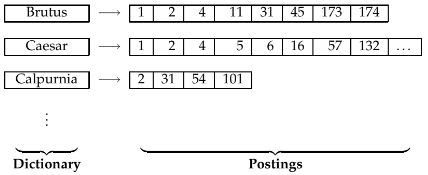
\includegraphics[width=\linewidth, height=2.5cm, keepaspectratio]{Pictures/info-retrieval/inverted-index.png}
    \caption{Inverted Index/ inverted file - example}
\end{figure}

\begin{enumerate}
    \item The name is actually redundant: an index always maps back from terms to the parts of a document where they occur. 
    
    \item \textbf{Inverted index}, or sometimes \textbf{inverted file}, has become the standard term in information retrieval.    
\end{enumerate}


\noindent \textbf{Steps}:
\begin{enumerate}
    \item \textbf{Collect} the documents to be indexed:\\
    \fbox{Friends, Romans, countrymen.} \fbox{So let it be with Caesar} $\cdots$

    \vspace{0.5cm}
    \item \textbf{Tokenize} the text, turning each document into a list of tokens:\\
    \fbox{Friends} \fbox{Romans} \fbox{countrymen} \fbox{So} \fbox{let} \fbox{it} \fbox{be} \fbox{with} \fbox{Caesar} $\cdots$

    \vspace{0.5cm}
    \item Do linguistic \textbf{preprocessing}, producing a list of normalized tokens, which are the indexing terms:\\
    \fbox{friend} \fbox{roman} \fbox{countryman} \fbox{so} $\cdots$

    \vspace{0.5cm}
    \item \textbf{Index} the documents that each term occurs in by creating an inverted index, consisting of a dictionary and postings.
\end{enumerate}


\noindent\textbf{Note}:
\begin{enumerate}
    \item each document has a \textbf{unique serial number}, known as the \textbf{document identifier}\indexlabel{docID: document identifier} ($docID$).\\
    During index construction, we can simply assign \textbf{successive integers} to each new document when it is first encountered.\\
    The input to indexing is a list of normalized tokens for each document, which we can equally think of as a list of pairs of term and $docID$.

    \item The core indexing step is \textbf{sorting} this list so that the terms are alphabetical.

    \item Multiple occurrences of the same term from the same document are then merged.

    \item Instances of the same term are then grouped, and the result is split into a dictionary and postings.

    \item Since a term generally occurs in a number of documents, this data organization already reduces the storage requirements of the index. 
    
    \item The dictionary also records some statistics, such as the number of documents which contain each term (the \textbf{document frequency}, which is here also the length of each postings list).

    \item The postings are secondarily sorted by $docID$.\\
    This provides the basis for efficient query processing.

    \item This inverted index structure is essentially without rivals as the most efficient structure for supporting ad hoc text search.

    \item In the resulting index, we pay for storage of both the dictionary and the postings lists.\\
    The latter are much larger, but the dictionary is commonly kept in \textbf{memory}, while postings lists are normally kept on \textbf{disk}, so the size of each is important.

    \item A fixed length array would be wasteful as some words occur in many documents, and others in very few. For an in-memory postings list, two good alternatives are \textbf{singly linked lists} or \textbf{variable length arrays}.
    \begin{enumerate}
        \item \textbf{Singly linked lists} allow cheap insertion of documents into postings lists, which require additional pointers.

        \item \textbf{Variable length arrays} win in space requirements by avoiding the overhead for pointers and in time requirements because their use of \textbf{contiguous memory} increases speed on modern processors with memory caches.\\
        Extra pointers can in practice be encoded into the lists as offsets.\\
        If updates are relatively infrequent, variable length arrays will be more compact and faster to traverse.

        \item We can also use a hybrid scheme with a linked list of fixed length arrays for each term.\\
        When postings lists are stored on disk, they are stored (perhaps compressed) as a contiguous run of postings without explicit pointers, so as to minimize the size of the postings list and the number of disk seeks to read a postings list into memory.
    \end{enumerate}

    
\end{enumerate}

\noindent \textbf{Example}:
\begin{table}[h]
    \begin{minipage}[t]{.45\linewidth}
        \textbf{Doc1}\\
        I did enact Julius Caesar: I was killed i’ the Capitol; Brutus killed me.
    \end{minipage}
    \hfill
    \begin{minipage}[t]{.45\linewidth}
        \textbf{Doc2}\\
        So let it be with Caesar. The noble Brutus hath told you Caesar was ambitious:
    \end{minipage}
    \caption{Inverted Index - Step 1}
\end{table}

\begin{table}[h]
    \begin{minipage}[t]{0.25\linewidth}
        \begin{table}[H]
            \centering
            \begin{tabular}{l r}
                \textbf{term} & \textbf{docID} \\
                I & 1 \\
                did & 1 \\
                enact & 1 \\
                $\vdots$ & $\vdots$ \\
                was & 2 \\
                ambitious & 2 \\
            \end{tabular}
            \caption{Inverted Index - Step 2}
        \end{table}
    \end{minipage}
    \hfill
    \begin{minipage}[t]{0.25\linewidth}
        \begin{table}[H]
            \centering
            \begin{tabular}{l r}
                \textbf{term} & \textbf{docID} \\
                ambitious & 2 \\
                be & 2 \\
                brutus & 1 \\
                $\vdots$ & $\vdots$ \\
                was & 2 \\
                with & 2 \\
            \end{tabular}
            \caption{Inverted Index - Step 3}
        \end{table}
    \end{minipage}
    \hfill
    \begin{minipage}[t]{0.4\linewidth}
        \begin{table}[H]
            \centering
            \begin{tabular}{l l c l}
                \textbf{term} & \textbf{doc. freq.} & $\to$ & \textbf{postings lists} \\
                \fbox{ambitious} & \fbox{1} & $\to$ & \fbox{2} \\
                \fbox{be} & \fbox{1} & $\to$ & \fbox{2} \\
                \fbox{brutus} & \fbox{2} & $\to$ & \fbox{1} $\to$ \fbox{2} \\
                $\vdots$ & $\vdots$ \\
                \fbox{was} & \fbox{2} & $\to$ & \fbox{1} $\to$ \fbox{2} \\
                \fbox{with} & \fbox{1} & $\to$ & \fbox{2} \\
            \end{tabular}
            \caption{Inverted Index - Step 4}
        \end{table}
    \end{minipage}
\end{table}































    \chapter{Artificial Intelligence (AI) \cite{aci-1}}

\begin{enumerate}[itemsep=0.2cm]
    \item The field of artificial intelligence, or AI, attempts not just to understand but also to build intelligent entities. 

    \item \textbf{Acting humanly}: \textit{Turing test}
    \begin{enumerate}
        \item The \textbf{Turing Test}\indexlabel{Turing Test}, proposed by Alan Turing (1950), was designed to provide a satisfactory operational definition of intelligence.\\
        A computer passes the test if a human interrogator, after posing some written questions, cannot tell whether the written responses come from a person or from a computer.\\
        total Turing Test includes a video signal so that the interrogator can test the subject’s perceptual abilities, as well as the opportunity for the interrogator to pass physical objects “through the hatch.”\\
        To pass the total Turing Test, the computer will need:
        \begin{enumerate}
            \item \textbf{computer vision} to perceive objects

            \item \textbf{robotics} to manipulate objects and move about
        \end{enumerate}

        \item The computer would need to possess the following capabilities: 
        \begin{enumerate}
            \item \textbf{natural language processing} to enable it to communicate successfully in English

            \item \textbf{knowledge representation} to store what it knows or hears

            \item \textbf{automated reasoning} to use the stored information to answer questions and to draw new conclusions

            \item \textbf{machine learning} to adapt to new circumstances and to detect and extrapolate patterns
        \end{enumerate}
    \end{enumerate}

    \item \textbf{Thinking humanly}: \textit{The cognitive modeling approach} 
    \begin{enumerate}
        \item The interdisciplinary field of \textbf{cognitive science}\indexlabel{cognitive science} brings together computer models from AI and experimental techniques from psychology to construct precise and testable theories of the human mind. 

        \item an algorithm performs well on a task and that it is therefore a good model of human performance, or vice versa.
    \end{enumerate}

    \item \textbf{Thinking rationally}: \textit{The “laws of thought” approach}
    \begin{enumerate}
        \item The Greek philosopher Aristotle was one of the first to attempt to codify “right thinking,” that is, irrefutable reasoning processes

        \item His syllogisms/ arguments provided patterns for argument structures that always yielded correct conclusions when given correct premises-for example, \textit{“Socrates is a man; all men are mortal; therefore, Socrates is mortal.”}

        \item logicist tradition within artificial intelligence hopes to build on such programs to create intelligent systems. \\
        There are two main obstacles to this approach.
        \begin{enumerate}
            \item it is not easy to take informal knowledge and state it in the formal terms required by logical notation, particularly when the knowledge is less than 100\% certain

            \item there is a big difference between solving a problem “in principle” and solving it in practice.
        \end{enumerate}
    \end{enumerate}

    \item \textbf{Acting rationally}: \textit{The rational agent approach}
    \begin{enumerate}
        \item An \textbf{agent}\indexlabel{agent} is just something that acts (agent comes from the Latin agere, to do).\\
        Of course, all computer programs do something, but computer agents are expected to do more: operate autonomously, perceive their environment, persist over a prolonged time period, adapt to change, and create and pursue goals. 
        
        \item A \textbf{rational agent}\indexlabel{rational agent} is one that acts so as to achieve the best outcome or, when there is uncertainty, the best expected outcome.

        \item In the \textit{“laws of thought” approach} to AI, the emphasis was on correct inferences.\\
        Making correct inferences is sometimes part of being a rational agent, because one way to act rationally is to reason logically to the conclusion that a given action will achieve one’s goals and then to act on that conclusion.\\
        On the other hand, correct inference is not all of ration-ality; in some situations, there is no provably correct thing to do, but something must still be done.\\
        There are also ways of acting rationally that cannot be said to involve inference.\\
        \textbf{For example}, recoiling from a hot stove is a reflex action that is usually more successful than a slower action taken after careful deliberation.

        \item The rational-agent approach has two advantages over the other approaches. 
        \begin{enumerate}
            \item it is more general than the “laws of thought” approach because correct inference is just one of several possible mechanisms for achieving rationality. 

            \item it is more amenable to scientific development than are approaches based on human behavior or human thought. 
        \end{enumerate}

        \item The standard of rationality is mathematically well defined and completely general, and can be “unpacked” to generate agent designs that provably achieve it.\\
        Human behavior, on the other hand, is well adapted for one specific environment and is defined by, well, the sum total of all the things that humans do.

        \item \textbf{limited rationality}\indexlabel{limited rationality} - acting appropriately when there is not enough time to do all the computations one might like.
    \end{enumerate}
\end{enumerate}

\section{Fundamentals of AI \cite{aci-1}}

\subsection{Philosophy}
\begin{enumerate}
    \item \textbf{rationalism}\indexlabel{rationalism} Descartes was a strong advocate of the power of reasoning in understanding the world, a philosophy now called rationalism, and one that counts Aristotle and Leibnitz as members. 

    \item \textbf{dualism}\indexlabel{dualism}: Descartes was also a proponent of dualism.\\
    He held that there is a part of the human mind (or soul or spirit) that is outside of nature, exempt from physical laws.\\
    Animals, on the other hand, did not possess this dual quality; they could be treated as machines.

    \item \textbf{materialism}\indexlabel{materialism}: An alternative to dualism is materialism, which holds that the brain’s operation according to the laws of physics constitutes the mind.\\
    Free will is simply the way that the perception of available choices appears to the choosing entity.

    \item \textbf{empiricism}\indexlabel{empiricism}: the theory that all knowledge is based on experience derived from the senses.

    \item \textbf{induction}\indexlabel{induction}: that general rules are acquired by exposure to repeated associations between their elements.

    \item \textbf{logical positivism}\indexlabel{logical positivism}: holds that all knowledge can be characterized by logical theories connected

    \item \textbf{confirmation theory}\indexlabel{confirmation theory}: to analyze the acquisition of knowledge from experience

    \item the mind is the connection between knowledge and action

    \item because intelligence requires action as well as reasoning

    \item only by understanding how actions are justified can we understand how to build an agent whose actions are justifiable (or rational)
\end{enumerate}

\subsection{Mathematics}
\begin{enumerate}
    \item leap to a formal science required a level of mathematical formalization in three fundamental areas: logic, computation, and probability.

    \subsubsection*{Logic}

    \item The idea of formal logic can be traced back to the philosophers of \textbf{ancient Greece} who worked out the details of propositional, or Boolean logic.

    \item In 1879, \textbf{Gottlob Frege} (1848–1925) extended Boole’s logic to include objects and relations, creating the \textit{first-order logic}\\
    first-order logic could \textbf{not} capture the principle of mathematical induction needed to characterize the natural numbers.

    \item \textbf{Alfred Tarski} (1902–1983) introduced a theory of reference that shows how to relate the objects in a logic to objects in the real world.

    \item \textbf{algorithm}: a process or set of rules to be followed in calculations or other problem-solving operations, especially by a computer.\\
    The first nontrivial algorithm is thought to be Euclid’s algorithm for computing greatest common divisors.

    \item In 1931, Godel showed that limits on deduction do exist.\\
    His \textbf{incompleteness theorem}\indexlabel{incompleteness theorem} showed that in any formal theory as strong as Peano arithmetic (the elementary theory of natural numbers), there are true statements that are undecidable in the sense that they have no proof within the theory. \\
    some functions on the integers cannot be represented by an algorithm - that is, they cannot be computed. \\
    the notion of a computation or effective procedure really cannot be given a formal definition

    \subsubsection*{Computation}

    \item \textbf{Church–Turing thesis}\indexlabel{Church–Turing thesis}, which states that the Turing machine (Turing, 1936) is capable of computing any computable function, is generally accepted as providing a sufficient definition.\\
    Turing also showed that there were some functions that no Turing machine can compute.\\
    \textbf{For example}, no machine can tell in general whether a given program will return an answer on a given input or run forever. 

    \item a problem is called \textbf{intractable} if the time required to solve instances of the problem grows exponentially with the size of the instances.\\
    It is important because exponential growth means that even moderately large instances cannot be solved in any reasonable time.\\
    Therefore, one should strive to divide the overall problem of generating intelligent behavior into tractable subproblems rather than intractable ones. 

    \item theory of \textbf{NP-completeness}: \textbf{Steven Cook} (1971) and \textbf{Richard Karp} (1972) showed the existence of large classes of canonical combinatorial search and reasoning problems that are NP-complete.\\
    Any problem class to which the class of NP-complete problems can be reduced is likely to be intractable. (Although it has not been proved that NP-complete problems are necessarily intractable)

    \subsubsection*{Probability}

    \item Italian \textbf{Gerolamo Cardano} (1501–1576) first framed the idea of \textbf{probability}, describing it in terms of the possible outcomes of gambling events.
\end{enumerate}

\subsection{Economics}
\begin{enumerate}
    \item Most people think of economics as being about money, but economists will say that they are really studying how people make choices that lead to preferred outcomes. 

    \item \textbf{utility}: useful, profitable, or beneficial\\
    The mathematical treatment of “preferred outcomes” or utility was first formalized by \textbf{Leon Walras} (1834-1910)

    \item \textbf{Decision theory}, which combines probability theory with utility theory, provides a formal and complete framework for decisions (economic or otherwise) made under uncertainty - that is, in cases where probabilistic descriptions appropriately capture the decision maker’s environment.\\
    This is suitable for \textit{“large” economies} where each agent need pay no attention to the actions of other agents as individuals.

    \item For \textit{“small” economies}, the situation is much more like a \textbf{game}: the actions of one player can significantly affect the utility of another (either positively or negatively).\\
    \textbf{Von Neumann} and \textbf{Morgenstern}’s development of \textbf{game theory} included the surprising result that, for some games, a rational agent should adopt policies that are (or least appear to be) randomized.\\
    Unlike decision theory, game theory does not offer an unambiguous prescription for selecting actions.

    \item The topic of \textit{"ow to make rational decisions when payoffs from actions are not immediate but instead result from several actions taken in sequence"} was pursued in the field of \textbf{operations research}, which emerged in World War II from efforts in Britain to optimize radar installations.\\
    The work of Richard Bellman (1957) formalized a class of sequential decision problems called \textbf{Markov decision processes} (MDP).

    \item models based on satisficing - making decisions that are “good enough,” rather than laboriously calculating an optimal decision - gave a better description of actual human behavior.
\end{enumerate}

\subsection{Neuroscience}
\begin{enumerate}
    \item Neuroscience is the study of the nervous system, particularly the brain.

    \item brain consisted of nerve cells, or neurons

    \item computers have a cycle time that is a million times faster than a brain.\\
    The brain makes up for that with far more storage and interconnection than even a high-end personal computer, although the largest supercomputers have a capacity that is similar to the brain’s.
\end{enumerate}

\subsection{Psychology}
\begin{enumerate}
    \item \textbf{Behaviorism movement}, led by \textbf{John Watson} (1878–1958), rejected any theory involving mental processes on the grounds that introspection could not provide reliable evidence. \\
    Behaviorists insisted on studying only objective measures of the percepts (or stimulus) given to an animal and its resulting actions (or response). 

    \item \textbf{Cognitive psychology} views the brain as an information-processing device.

    \item Helmholtz also insisted that perception involved a form of \textit{unconscious logical inference}.

    \item Craik specified the three key steps of a \textbf{knowledge-based agent}: 
    \begin{enumerate}
        \item the stimulus must be translated into an internal representation
        \item the representation is manipulated by cognitive processes to derive new internal representations
        \item these are in turn re-translated back into action
    \end{enumerate}

    
\end{enumerate}

\subsection{Computer engineering}
\begin{enumerate}
    \item each generation of computer hardware has brought an increase in speed and capacity and a decrease in price.

    \item power dissipation problems led manufacturers to start multiplying the number of CPU cores rather than the clock speed.

    \item \textbf{Charles Babbage} (1792–1871) designed two machines, neither of which he com-pleted.
    \begin{enumerate}
        \item The \textbf{Difference Engine} was intended to compute mathematical tables for engineering and scientific projects. 

        \item \textbf{Analytical Engine} was far more ambitious: it included addressable memory, stored programs, and conditional jumps and was the first artifact capable of universal computation.
    \end{enumerate}

    \item software side of computer science: work in AI has pioneered many ideas that have made their way back to mainstream computer science, including time sharing, interactive interpreters, personal computers with windows and mice, rapid development environments, the linked list data type, automatic storage management, and key concepts of symbolic, functional, declarative, and object-oriented programming.
\end{enumerate}

\subsection{Control theory and cybernetics}
\begin{enumerate}
    \item \textbf{Control theory} is a field of control engineering and applied mathematics that deals with the control of dynamical systems in engineered processes and machines. \cite{wiki/Control_theory}
    
    \item The objective is to develop a model or algorithm governing the application of system inputs to drive the system to a desired state, while minimizing any delay, overshoot, or steady-state error and ensuring a level of control stability; often with the aim to achieve a degree of optimality. \cite{wiki/Control_theory}

    \item \textbf{Cybernetics} is the trans-disciplinary study of circular processes such as feedback systems where outputs are also inputs. \cite{wiki/Cybernetics}

    \item intelligence could be created by the use of homeostatic devices containing appropriate feedback loops to achieve stable adaptive behavior

    \item Modern control theory, especially the branch known as \textbf{stochastic optimal control}, has as its goal the design of systems that maximize an objective function over time.

    \item Calculus and matrix algebra, the tools of control theory, lend themselves to systems that are describable by fixed sets of continuous variables, whereas AI was founded in part as a way to escape from the these perceived limitations. 
\end{enumerate}

\subsection{Linguistics}
\begin{enumerate}
    \item \textbf{Noam Chomsk} pointed out that the behaviorist theory did not address the notion of \textit{creativity} in language-it did not explain how a child could understand and make up sentences that he or she had never heard before. 

    \item Understanding language requires an understanding of the subject matter and context, not just an understanding of the structure of sentences.

    \item \textbf{knowledge representation}\indexlabel{knowledge representation}: the study of how to put knowledge into a form that a computer can reason with
\end{enumerate}



\section{Components of AI}

\begin{figure}[H]
    \centering
    \includegraphics[width=\linewidth, height=3cm, keepaspectratio]{Pictures/ai-ml/agent-env-skeleton.png}
    \caption*{Agents interact with environments through sensors and actuators \cite{aci-1}}
\end{figure}

\begin{enumerate}
    \item An \textbf{agent} is anything that can be viewed as perceiving its \textbf{environment} through \textbf{sensors} and acting upon that environment through \textbf{actuators}.

    \item notion of desirability is captured by a \textbf{performance measure} that evaluates any given sequence of environment states.

    \item As a general rule, it is better to design performance measures according to what one actually wants in the environment, rather than according to how one thinks the agent should behave. 

    \item \textbf{information gathering}: Doing actions in order to modify future percepts
\end{enumerate}


\subsection{Agent}

\begin{enumerate}
    \item Mathematically speaking, we say that an agent’s behavior is described by the \textbf{agent function}\indexlabel{agent function} that maps any given percept sequence to an action.\\
    This an external characterization of the agent.

    \item Internally, the agent function for an artificial agent will be implemented by an \textbf{agent program}\indexlabel{agent program}.

    \item[] The agent function is an abstract mathematical description; the agent program is a concrete implementation, running within some physical system.\\
    SEE: \fullref{Agent Function VS Agent Program}

    \item A \textbf{rational agent} is one that does the right thing-conceptually speaking, every entry in the table for the agent function is filled out correctly. \\
    For each possible percept sequence, a rational agent should select an action that is expected to maximize its performance measure, given the evidence provided by the percept sequence and whatever built-in knowledge the agent has.

    \item An \textbf{omniscient agent} knows the actual outcome of its actions and can act accordingly; but omniscience is impossible in reality. 

    \item Rationality maximizes expected performance, while perfection maximizes actual performance.

    \item To the extent that an agent relies on the prior knowledge of its designer rather than on its own percepts, we say that the agent lacks \textbf{autonomy}.\\
    A rational agent should be autonomous-it should learn what it can to compensate for partial or incorrect prior knowledge. 
\end{enumerate}


\subsection{Environment}

\begin{enumerate}
    \item The environment is the external system or world in which the agent operates. It provides inputs (percepts) to the agent and reacts to the agent's actions. \cite{chatgpt}

    \item The “geography” of the environment is known \textbf{"a priori"} 
\end{enumerate}


\subsection{Sensor (input device) \cite{chatgpt}}

\begin{enumerate}
    \item A sensor is a device that allows an agent to perceive its environment. 
    
    \item It collects information from the environment, such as a camera capturing images or a thermometer measuring temperature.
\end{enumerate}


\subsection{Actuator (output device) \cite{chatgpt}}

\begin{enumerate}
    \item An actuator is a mechanism or device that the agent uses to take physical actions in the environment. 
    
    \item For example, in robotics, motors and servos are actuators that move parts of the robot.
\end{enumerate}


\subsection{Percepts (input)}

\begin{enumerate}
    \item \textbf{percept} refers to the agent’s perceptual inputs at any given instant

    \item \textbf{percept sequence} is the complete history of everything the agent has ever perceived

\end{enumerate}


\subsection{Actions (output)}

\begin{enumerate}
    \item an agent’s choice of action at any given instant can depend on the entire percept sequence observed to date, but not on anything it hasn’t perceived
\end{enumerate}



\section{Task Environment}

\begin{enumerate}
    \item task environments are essentially the “problems” to which rational agents are the “solutions.”

    \item "task environment" means "environment of task" in literal sense, but it actually means "scenario of task" or "task ecosystem"
\end{enumerate}

\subsection{PEAS description of task environment}
\begin{enumerate}
    \item P - Performance
    \item E - Environment
    \item A - Actuators
    \item S - Sensors
\end{enumerate}

Example:
\begin{customTableWrapper}{1.2}
\begin{table}[H]
    \centering
    \begin{tabular}{|l p{10cm}|}
        \hline
        \textbf{Task Environment} & automated taxi \\
        \hline\hline
        
        \textbf{Agent} & Taxi driver \\
        \hline

        \textbf{Performance Measure} & Safe, fast, legal, comfortable trip, maximize profits \\

        \textbf{Environment} & Roads, other traffic, pedestrians, customers \\

        \textbf{Actuators} & Steering, accelerator, brake, signal, horn, display \\

        \textbf{Sensors} & Cameras, sonar, speedometer, GPS, odometer, accelerometer, engine sensors, keyboard \\
        \hline
    \end{tabular}
\end{table}
\end{customTableWrapper}

\subsection{Properties of Task Environments}

\subsubsection{Observability}
\begin{enumerate}
    \item \textbf{Fully observable environment}: agent’s sensors give it access to the complete state of the environment at each point in time\\
    A task environment is effectively fully observable if the sensors detect all aspects that are relevant to the choice of action; relevance, in turn, depends on the performance measure.\\
    Fully observable environments are convenient because the agent need not maintain any internal state to keep track of the world. 

    \item \textbf{Partially observable environment}: An environment might be partially observable because of noisy and inaccurate sensors or because parts of the state are simply missing from the sensor data.

    \item \textbf{un-observable environment}: If the agent has no sensors at all then the environment is un-observable.\\
    One might think that in such cases the agent’s plight is hopeless, but the agent’s goals may still be achievable, sometimes with certainty. 

\end{enumerate}


\subsubsection{Single Agent VS Multi-agent}
\begin{enumerate}
    \item \textbf{Single Agent}: Only one agent operates on the environment.\\
    \textbf{For example}: an agent solving a crossword puzzle by itself is clearly in a single-agent environment. 

    \item \textbf{Multi-agent}: Multiple agents operate on same environment.\\
    \textbf{communication} often emerges as a rational behavior in multi-agent environments

    \begin{enumerate}
        \item \textbf{Competitive multi-agent environment}: multiple agents compete against each other for their own benefits\\
        in some competitive environments, \textbf{randomized behavior} is rational because it avoids the pitfalls of predictability\\
        \textbf{Example}: chess

        \item \textbf{Cooperative multi-agent environment}: multiple agents cooperate with each other for mutual benefits\\
        \textbf{Example}: multiple self driving cars in same environment
    \end{enumerate}
\end{enumerate}


\subsubsection{Deterministic VS stochastic}
\begin{enumerate}
    \item if next state of the environment is completely determined by the current state and the action executed by the agent, otherwise stochastic.

    \item \textbf{Non-deterministic}: which actions are characterized by their possible outcomes, but no probabilities are attached to them\\
    Non-deterministic environment descriptions are usually associated with performance measures that require the agent to succeed for all possible outcomes of its actions.
\end{enumerate}


\subsubsection{Uncertainty}
\begin{enumerate}
    \item an agent need not worry about \textbf{uncertainty} in a fully observable, deterministic environment

    \item We say an environment is \textbf{uncertain} if it is not fully observable or not deterministic.
\end{enumerate}


\subsubsection{Episodic VS sequential}

\begin{enumerate}
    \item \textbf{Episodic}: In an episodic task environment, the agent’s experience is divided into atomic episodes.\\
    In each episode the agent receives a percept and then performs a single action.\\
    Next episode does not depend on the actions taken in previous episodes.\\
    Episodic environments are much simpler than sequential environments because the agent does not need to think ahead.

    \item \textbf{Sequential}: In sequential environments, on the other hand, the current decision could affect all future decisions.
\end{enumerate}


\subsubsection{Static VS dynamic}
\begin{enumerate}
    \item If the environment can change while an agent is deliberating, then we say the environment is \textbf{dynamic} for that agent; otherwise, it is \textbf{static}.

    \item Static environments are easy to deal with because the agent need not keep looking at the world while it is deciding on an action, nor need it worry about the passage of time.\\
    \textbf{Example}: Crossword puzzles are static.

    \item Dynamic environments, on the other hand, are continuously asking the agent what it wants to do; if it hasn’t decided yet, that counts as deciding to do nothing. \\
    \textbf{Example}: Taxi driving is clearly dynamic: the other cars and the taxi itself keep moving while the driving algorithm dithers about what to do next.

    \item If the environment itself does not change with the passage of time but the agent’s performance score does, then we say the environment is \textbf{semi-dynamic}. \\
    \textbf{Example}: Chess, when played with a clock, is semi-dynamic.
\end{enumerate}


\subsubsection{Discrete vs. continuous}
\begin{enumerate}
    \item The discrete/continuous distinction applies to the state of the environment, to the way \textbf{time} is handled, and to the percepts and actions of the agent.

\paragraph*{Examples:}

    \item the chess environment has a finite number of distinct states (excluding the clock).\\
    Chess also has a discrete set of percepts and actions. 
    
    \item Taxi driving is a continuous-state and continuous-time problem: the speed and location of the taxi and of the other vehicles sweep through a range of continuous values and do so smoothly over time.\\
    Taxi-driving actions are also continuous (steering angles, etc.).\\
    Input from digital cameras is discrete, strictly speaking, but is typically treated as representing continuously varying intensities and locations.
\end{enumerate}


\subsubsection{Known vs. unknown}
\begin{enumerate}
    \item this distinction refers not to the environment itself but to the agent’s (or designer’s) state of knowledge about the “laws of physics” of the environment.

    \item In a \textbf{known environment}, the outcomes (or outcome probabilities if the environment is stochastic) for all actions are given.\\
    not the same as fully observable environments: It is quite possible for a known environment to be partially observable - for example, in solitaire card games, I know the rules but am still unable to see the cards that have not yet been turned over.

    \item if the environment is \textbf{unknown}, the agent will have to learn how it works in order to make good decisions.\\
    not the same as partially observable environments: an unknown environment can be fully observable - in a new video game, the screen may show the entire game state but I still don’t know what the buttons do until I try them. 
\end{enumerate}


\subsubsection*{Note}
\begin{enumerate}
    \item the hardest case is partially observable, multi-agent, stochastic, sequential, dynamic, continuous,and unknown.\\
    Taxi driving is hard in all these senses, except that for the most part the driver’s environment is known.\\
    Driving a rented car in a new country with unfamiliar geography and traffic laws is a lot more exciting. 

    \item \textbf{environment class}\indexlabel{environment class}: collection of environments

    \item \textbf{environment generator}: that selects particular environments (with certain likelihoods) in which to run the agent
\end{enumerate}

Examples of task environments and their characteristics \cite{aci-1}:
\begin{customTableWrapper}{1.2}
\begin{longtable}{|l|llllll|}
    \customTableHeaderColor
    \hline
    \textbf{Task Environment} & \textbf{Observable} & \textbf{Agents} & \textbf{Deterministic} & \textbf{Episodic} & \textbf{Static} & \textbf{Discrete} \\ 
    \hline\hline
    \endfirsthead

    \hline\endhead
    \hline\endfoot
    \hline\endlastfoot

    Crossword puzzle & Fully &  Single &  Deterministic & Sequential & Static & Discrete \\
    Chess with a clock & Fully & Multi & Deterministic & Sequential & Semi & Discrete \\
    
    \hline
    
    Poker & Partially & Multi & Stochastic & Sequential & Static&  Discrete \\
    Backgammon & Fully& Multi& Stochastic& Sequential& Static& Discrete\\
    
    \hline
    
    Taxi driving & Partially& Multi&  Stochastic& Sequential& Dynamic& Continuous\\
    Medical diagnosis& Partially & Single & Stochastic& Sequential& Dynamic& Continuous\\
    
    \hline
    
    Image analysis & Fully& Single& Deterministic& Episodic& Semi& Continuous\\
    Part-picking robot & Partially& Single& Stochastic& Episodic& Dynamic& Continuous\\
    
    \hline
    
    Refinery controller& Partially& Single& Stochastic& Sequential& Dynamic& Continuous\\
    Interactive English tutor & Partially& Multi& Stochastic& Sequential& Dynamic& Discrete\\

\end{longtable}
\end{customTableWrapper}


\chapter{AI Agents \cite{aci-1}}

\begin{center}
    \texttt{agent = architecture + program}
\end{center}

\begin{enumerate}
    \item \textbf{architecture}: computing device with physical sensors and actuators\\
    In general, the architecture makes the percepts from the sensors available to the program, runs the program, and feeds the program’s action choices to the actuators as they are generated.
    
    \item The job of AI is to design an \textbf{agent program} that implements the agent function - the mapping from percepts to actions.\\
    the program we choose has to be one that is appropriate for the architecture.\\
    If the program is going to recommend actions like Walk, the architecture had better have legs. 
\end{enumerate}

\section{Agent State Representation \cite{aci-1}}

\begin{figure}[H]
    \centering
    \includegraphics[width=\linewidth, height=2.5cm, keepaspectratio]{Pictures/ai-ml/agent-state-repr.png}
    \caption*{atomic, factored, and structured states}
\end{figure}

\begin{enumerate}
    \item \textbf{Atomic}
    \begin{enumerate}
        \item each state of the world is indivisible—it has no internal structure. 
    
        \item The algorithms underlying search and game-playing, Hidden Markov models, and Markov decision processes all work with atomic representations—or, at least, they treat representations as if they were atomic.

        \item if two different atomic states have nothing in common—they are just different black boxes
    \end{enumerate}

    \item \textbf{Factored}
    \begin{enumerate}
        \item A factored representation splits up each state into a fixed set of \textbf{variables} or \textbf{attributes}, each of which can have a \textbf{value}.

        \item two different factored states can share some attributes and not others; this makes it much easier to work out how to turn one state into another.

        \item With factored representations, we can also represent uncertainty\\
        \textbf{for example}, ignorance about the amount of gas in the tank can be represented by leaving that attribute blank.

        \item  Many important areas of AI are based on factored representations, including constraint satisfaction algorithms, propositional logic, planning, Bayesian networks, and the machine learning algorithms.
    \end{enumerate}

    \item \textbf{structured}
    \begin{enumerate}
        \item we need to understand the world as having things in it that are
related to each other, not just variables with values.

        \item Structured representations underlie relational databases and first-order logic, first-order probability models, knowledge-based learning and much of natural language understanding. 
        
        \item almost everything that humans express in natural language concerns objects and their relationships.
    \end{enumerate}

    \item  the axis along which atomic, factored, and structured representations lie is the axis of increasing \textbf{expressiveness}.\\
    a more expressive representation can capture, at least as concisely, everything a less expressive one can capture, plus some more.\\
    Often, the more expressive language is much more concise; for example, the rules of chess can be written in a page or two of a structured-representation language such as first-order logic but require thousands of pages when written in a factored-representation language such as propositional logic.\\
    On the other hand, reasoning and learning become more complex as the expressive power of the representation increases.\\
    To gain the benefits of expressive representations while avoiding their drawbacks, intelligent systems for the real world may need to operate at all points along the axis simultaneously.
\end{enumerate}

\section{Agent programs \cite{aci-1}}

\begin{enumerate}
    \item skeleton: they take the current percept as input from the sensors and return an action to the actuators. 
    
    \item agent program takes the current percept as input\\
    he agent program takes just the current percept as input because nothing more is available from the environment; if the agent’s actions need to depend on the entire percept sequence, the agent will have to remember the percepts.

    \item agent function takes the entire percept history
\end{enumerate}

\subsection{Table Driven Agent \cite{aci-1}}

\begin{algorithm}[H]
    \caption{The TABLE-DRIVEN-AGENT program is invoked for each new percept and returns an action each time. It retains the complete percept sequence in memory. \cite{aci-1}}

    \SetKwFunction{FUNCTION}{TABLE-DRIVEN-AGENT}
    \SetKwProg{Fn}{function}{:}{}
    \Fn{\FUNCTION{percept}}{
        \textbf{persistent}:\\
        \hspace{0.4cm} \textit{percepts}, a sequence, initially empty\\
        \hspace{0.4cm} \textit{table}, a table of actions, indexed by percept sequences, initially fully specified \\
        append \textit{percept} to the end of \textit{percepts} \\
        \textit{action} $\gets$ LOOKUP(\textit{percepts},\textit{table}) \\
        \Return \textit{action}
    }
\end{algorithm}

\vspace{0.3cm}

\begin{enumerate}
    \item If $\mathcal{P}$ be the set of possible percepts and let $\mathcal{T}$ be the lifetime of the agent (the total number of percepts it will receive), then The lookup table will contain $\dsum^T_{t=1} |P| ^t$ entries.

    \item Challenges if there are too many table entries:
    \begin{enumerate}
        \item storage space
        \item designer need time to create the table
        \item agent might never learn all the right table entries from its experience
        \item even if the environment is simple enough to yield a feasible table size, the designer still has no guidance about how to fill in the table entries
    \end{enumerate}

\end{enumerate}

\subsection{Simple reflex agents \cite{aci-1}}

\begin{table}[H]
    \begin{minipage}{0.4\linewidth}
        \begin{figure}[H]
            \centering
            \includegraphics[width=\linewidth, height=4cm, keepaspectratio]{Pictures/ai-ml/agent--simple-reflex.png}
            \caption{Schematic diagram of a simple reflex agent}
        \end{figure}
    \end{minipage}
    \hfill
    \begin{minipage}{0.58\linewidth}
        \begin{algorithm}[H]
            \caption{simple reflex agent \cite{aci-1}}

            \SetKwFunction{FUNCTION}{SIMPLE-REFLEX-AGENT}
            \SetKwProg{Fn}{function}{:}{}
            \Fn{\FUNCTION{percept}}{
                \textbf{persistent}: \textit{rules}, a set of condition–action rules\\

                \textit{state} $\gets$ INTERPRET-INPUT(\textit{percept}) \\
                
                \textit{rule} $\gets$ RULE-MATCH(\textit{state,rules}) \\
                
                \textit{action} $\gets$ \textit{rule}.ACTION \\
                
                \textbf{return} \textit{action}
            }
        \end{algorithm}
    \end{minipage}
\end{table}

\vspace{0.3cm}

\begin{enumerate}
    \item The simplest kind of agent is the simple reflex agent. 
    
    \item These agents select actions on the basis of the current percept, ignoring the rest of the percept history.

    \item uses \textbf{condition–action rules} to map percepts to actions

    \item The \textbf{INTERPRET-INPUT function} generates an abstracted description of the current state from the percept, and the \textbf{RULE-MATCH function} returns the first rule in the set of rules that matches the given state description.

    \item Note that the description in terms of “rules” and “matching” is purely conceptual; actual implementations can be as simple as a collection of logic gates implementing a Boolean circuit.

\subsubsection*{DISADVANTAGES:}

    \item limited intelligence
    
    \item environment needs to be fully observable. Even a little bit of unobservability can cause serious trouble.
    
    \item Infinite loops are often unavoidable for simple reflex agents operating in partially observable environments\\
    \textbf{Solution}: Escape from infinite loops is possible if the agent can randomize its actions.\\
    In single-agent environments, randomization is usually not rational.\\
    It is a useful trick that helps a simple reflex agent in some situations, but in most cases we can do much better with more sophisticated deterministic agents. 
\end{enumerate}



\subsection{Model-based reflex agents \cite{aci-1}}

\begin{table}[H]
    \begin{minipage}{0.4\linewidth}
        \begin{figure}[H]
            \centering
            \includegraphics[width=\linewidth, height=4cm, keepaspectratio]{Pictures/ai-ml/agent--model-based-reflex.png}
            \caption{Model-based reflex agent}
        \end{figure}
    \end{minipage}
    \hfill
    \begin{minipage}{0.58\linewidth}
        \begin{algorithm}[H]
            \caption{model-based reflex agent \cite{aci-1}}

            \SetKwFunction{FUNCTION}{MODEL-BASED-REFLEX-AGENT}
            \SetKwProg{Fn}{function}{:}{}
            \Fn{\FUNCTION{percept}}{
                \textbf{persistent}:\\
                
                \hspace{0.4cm} \textit{state}, the agent’s current conception of the world state \\
                \hspace{0.4cm} \textit{model}, a description of how the next state depends on current state and action \\
                \hspace{0.4cm} \textit{rules}, a set of condition–action rules \\
                \hspace{0.4cm} \textit{action}, the most recent action, initially none \\

                \textit{state} $\gets$ UPDATE-STATE(\textit{state, action, percept, model}) \\
                
                \textit{rule} $\gets$ RULE-MATCH(\textit{state, rules}) \\
                
                \textit{action} $\gets$ \textit{rule}.ACTION \\
                
                \textbf{return} \textit{action}
            }
        \end{algorithm}
    \end{minipage}
\end{table}

\vspace{0.3cm}


\begin{enumerate}
    \item keeps track of the part of the world it can’t see now. (handle partial observability)\\
    The agent maintains some sort of \textbf{internal state} that depends on the percept history and thereby reflects at least some of the unobserved aspects of the current state.

    \item Updating this internal state information as time goes by requires two kinds of knowledge to be encoded in the agent program.
    \begin{enumerate}
        \item we need some information about how the world evolves independently of the agent

        \item we need some information about how the agent’s own actions affect the world
    \end{enumerate}
    This knowledge about “\textit{how the world works}” is called a \textbf{model} of the world. 

    \item The details of how models and states are represented vary widely depending on the type of environment and the particular technology used in the agent design. 

    \item Regardless of the kind of representation used, it is seldom possible for the agent to determine the current state of a partially observable environment exactly.\\
    Instead, the box\ mechanism labeled “what the world is like now” represents the agent’s “best guess” (or sometimes best guesses).
\end{enumerate}


\subsection{(Model-based) Goal-based agents \cite{aci-1}}

\begin{enumerate}
    \item as well as a current state description, the agent needs some sort of \textbf{goal} information that describes situations that are desirable

    \item \textbf{Search} and \textbf{planning} are the subfields of AI devoted to finding action sequences that achieve the agent’s goals.

    \item Although the goal-based agent appears less efficient, it is more flexible because the knowledge that supports its decisions is represented explicitly and can be modified.\\
    If it starts to rain, the agent can update its knowledge of how effectively its brakes will operate; this will automatically cause all of the relevant behaviors to be altered to suit the new conditions.\\
    For the reflex agent, on the other hand, we would have to rewrite many condition–action rules. 

    \item Goals alone are not enough to generate high-quality behavior in most environments.
\end{enumerate}


\begin{table}[h]
    \begin{minipage}{0.49\linewidth}
        \begin{figure}[H]
            \centering
            \includegraphics[width=\linewidth, height=4cm, keepaspectratio]{Pictures/ai-ml/agent--model-based-goal-based.png}
            \caption{Model-based goal-based agent \cite{aci-1}}
        \end{figure}
    \end{minipage}
    \hfill
    \begin{minipage}{0.49\linewidth}
        \begin{figure}[H]
            \centering
            \includegraphics[width=\linewidth, height=4cm, keepaspectratio]{Pictures/ai-ml/agent--model-based-utility-based.png}
            \caption{Model-based utility-based agent \cite{aci-1}}
        \end{figure}
    \end{minipage}
\end{table}

\subsection{Utility-based agents \cite{aci-1}}

\begin{enumerate}
    \item Many action sequences can lead to same goal, but some sequences are more favourable than others.\\
    Goals just provide a crude binary distinction between “happy” and “unhappy” states.\\
    A more general performance measure should allow a comparison of different world states according to exactly how happy they would make the agent.\\
    Because “happy” does not sound very scientific, economists and computer scientists use the term \textbf{utility} instead.

    \item An agent’s \textbf{utility function} is essentially an internalization of the performance measure. 
    
    \item If the internal utility function and the external performance measure are in agreement, then an agent that chooses actions to maximize its utility will be rational according to the external performance measure. 

    \item like goal-based agents, a utility-based agent has many advantages in terms of flexibility and learning.

    \item in two kinds of cases, goals are inadequate but a utility-based agent can still make rational decisions. 
    \begin{enumerate}
        \item when there are conflicting goals, only some of which can be achieved (for example, speed and safety), the utility function specifies the appropriate tradeoff.

        \item when there are several goals that the agent can aim for, none of which can be achieved with certainty, utility provides a way in which the likelihood of success can be weighed against the importance of the goals. 
    \end{enumerate}

    \item An agent that possesses an \textbf{\textit{explicit} utility function} can make rational decisions with a general-purpose algorithm that does not depend on the specific utility function being maximized.\\
    In this way, the “global” definition of rationality—designating as rational those agent functions that have the highest performance—is turned into a “local” constraint on rational-agent designs that can be expressed in a simple program.

    \item A utility-based agent has to model and keep track of its environment, tasks that have involved a great deal of research on perception, representation, reasoning, and learning. \\
    Choosing the utility-maximizing course of action is also a difficult task, requiring ingenious algorithms.
\end{enumerate}


\subsection{Learning Agent \cite{aci-1}}

\begin{figure}[H]
    \centering
    \includegraphics[width=\linewidth, height=4cm, keepaspectratio]{Pictures/ai-ml/agent--learning.png}
    \caption{General Learning Agent \cite{aci-1}}
\end{figure}


\begin{enumerate}
    \item Learning allows the agent to operate in initially unknown environments and to become more competent than its initial knowledge alone might allow.

    \item A learning agent can be divided into four conceptual components:
    \begin{enumerate}
        \item \textbf{learning element}: responsible for making improvements

        \item \textbf{performance element}: responsible for selecting external actions\\
        it takes in percepts and decides on actions

        \item \textbf{critic}: provides feedback on how the agent is doing and determines how the performance element should be modified to do better in the future\\
        The critic tells the learning element how well the agent is doing with respect to a fixed performance standard.\\
        The critic is necessary because the percepts themselves provide no indication of the agent’s success.

        \item \textbf{problem generator}: It is responsible for suggesting actions that will lead to new and informative experiences.\\
        The point is that if the performance element had its way, it would keep doing the actions that are best, given what it knows.\\
        But if the agent is willing to explore a little and do some perhaps sub-optimal actions in the short run, it might discover much better actions for the long run.\\
        The problem generator’s job is to suggest these exploratory actions.
    \end{enumerate}

    \item  the \textbf{performance standard} distinguishes part of the
incoming percept as a reward (or penalty) that provides direct feedback on the quality of the
agent’s behavior.    
\end{enumerate}



\subsection{problem-solving agent \cite{aci-1}}

\begin{enumerate}
    \item Problem-solving agents use \textbf{atomic} representations, states of the world are considered as wholes, with no internal structure visible to the problem-solving algorithms. 

    \item \textbf{uninformed search algorithms}—algorithms that are given no information about the problem other than its definition.

    \item \textbf{Informed search algorithms} can do quite well given some guidance on where to look for solutions

    \item \textbf{Goals} help organize behavior by limiting the objectives that the agent is trying to achieve and hence the actions it needs to consider.\\
    \textbf{Goal formulation}, based on the current situation and the agent’s performance measure, is the first step in problem solving.\\
    We consider a goal to be a set of world states—exactly those states in which the goal is satisfied.\\
    The agent’s task is to find out how to act, now and in the future, so that it reaches a goal state.

    \item  \textbf{Problem formulation} is the process of deciding what actions and states to consider, given a goal. 

    \item The process of looking for a sequence of actions that reaches the goal is called \textbf{search}.

    \item A search algorithm takes a problem as input and returns a \textbf{solution} in the form of an \textbf{action sequence}.\\
    Solution quality is measured by the path cost function, and an \textbf{optimal solution} has the lowest path cost among all solutions.

    \item Once a solution is found, the actions it recommends can be carried out. This is called the \textbf{execution phase}.

    \item A \textbf{problem} can be defined formally by five components:
    \begin{enumerate}
        \item The \textbf{initial state} that the agent starts in.

        \item A description of the possible \textbf{actions} available to the agent.\\
        Given a particular state \textit{s}, \verb|ACTIONS(s)| returns the set of actions that can be executed in \textit{s}.\\
        We say that each of these actions is \textbf{applicable} in \textit{s}.

        \item A description of what each action does; the formal name for this is the \textbf{transition model}, specified by a function \verb|RESULT(s, a)| that returns the state that results from doing action \textit{a} in state \textit{s}.\\
        We also use the term \textbf{successor} to refer to any state reachable from a given state by a single action.\\
        Together, the initial state, actions, and transition model implicitly define the \textbf{state space} of the problem—the set of all states reachable from the initial state by any sequence of actions.\\
        The state space forms a directed network or graph in which the nodes are states and the links between nodes are actions.\\
         A \textbf{path} in the state space is a sequence of states connected by a sequence of actions.

        \item \textbf{goal test} determines whether a given state is a goal state.

        \item The \textbf{step cost} of taking action $a$ in state $s$ to reach state $s'$ is denoted by $c(s, a, s')$.\\
        A \textbf{path cost} function that assigns a numeric cost to each path.\\
        The problem-solving agent chooses a cost function that reflects its own performance measure.\\
        we assume that the cost of a path can be described as the \textbf{sum} of the costs of the individual actions along the path.
    \end{enumerate}

    \item A \textbf{toy problem}\indexlabel{toy problem} is intended to illustrate or exercise various problem-solving methods.\\
    It can be given a concise, exact description and hence is usable by different researchers to compare the performance of algorithms.

    \item A \textbf{real-world problem}\indexlabel{real-world problem} is one whose solutions people actually care about.\\
    Such problems tend not to have a single agreed-upon description, but we can give the general flavor of their formulations.
\end{enumerate}

\begin{figure}[H]
    \centering
    \includegraphics[width=\linewidth, height=6cm, keepaspectratio]{Pictures/ai-ml/vaccum-toy-states.png}
    \caption*{The state space for the vacuum world. Links denote actions: L = Left, R = Right, S = Suck.}
\end{figure}

\begin{customTableWrapper}{1.3}
\begin{longtable}{|p{3cm} p{10cm}|}
    \hline\endfirsthead
    \hline\endhead
    \hline\endfoot
    \hline\endlastfoot

    \textbf{States} & The state is determined by both the agent location and the dirt locations. \\ 
    \hline

    \textbf{Initial state} & Any state can be designated as the initial state.\\
    \hline

    \textbf{Actions} & In this simple environment, each state has just three actions: Left, Right, and Suck.\\
    \hline

    \textbf{Transition model} & The actions have their expected effects, except that moving Left in the leftmost square, moving Right in the rightmost square, and Sucking in a clean square have no effect. \\
    \hline

    \textbf{Goal test} & This checks whether all the squares are clean.\\
    \hline

    \textbf{Path cost} & Each step costs 1, so the path cost is the number of steps in the path.\\
    \hline
\end{longtable}
\end{customTableWrapper}

\begin{algorithm}[h]
    \caption*{A simple problem-solving agent. It first formulates a goal and a problem, searches for a sequence of actions that would solve the problem, and then executes the actions one at a time. When this is complete, it formulates another goal and starts over. \cite{aci-1}}

    \SetKwFunction{FUNCTION}{SIMPLE-PROBLEM-SOLVING-AGENT}
    \SetKwProg{Fn}{function}{:}{}
    \Fn{\FUNCTION{percept}}{
        \textbf{persistent}:\\
        \hspace{0.4cm} \textit{seq}, an action sequence, initially empty \\
        \hspace{0.4cm} \textit{state}, some description of the current world state \\
        \hspace{0.4cm} \textit{goal}, a goal, initially null \\
        \hspace{0.4cm} \textit{problem}, a problem formulation\\
        
        state $\gets$ UPDATE-STATE(\textit{state, percept})\\
        \If{\textit{seq} is empty}{
            \textit{goal} $\gets$ FORMULATE-GOAL(\textit{state})\\
            
            \textit{problem} $\gets$ FORMULATE-PROBLEM(\textit{state, goal})\\
            
            \textit{seq} $\gets$ SEARCH(\textit{problem})\\
            
            \If{\textit{seq} = \textit{failure}}{
                \textbf{return} a null action
            }
        }
        \textit{action} $\gets$ FIRST(\textit{seq})\\
        \textit{seq} $\gets$ REST(\textit{seq})\\
        \textbf{return} \textit{action}
    }
\end{algorithm}


\subsubsection{Measuring problem-solving performance \cite{aci-1}}

\begin{customTableWrapper}{1.2}
\begin{table}[H]
    \centering
    \begin{tabular}{l p{10cm}}
        \textbf{Completeness} & Is the algorithm guaranteed to find a solution when there is one? \\
        
        \textbf{Optimality} & Does the strategy find the optimal solution? \\
        
        \textbf{Time complexity} & How long does it take to find a solution? \\
        
        \textbf{Space complexity} & How much memory is needed to perform the search?\\
    \end{tabular}
\end{table}
\end{customTableWrapper}


\begin{customTableWrapper}{1.2}
\begin{table}[H]
    \centering
    \begin{tabular}{l p{10cm}}
        $V$ & set of vertices (nodes) of the graph \\
        
        $E$ & set of edges (links) \\

        $b$ & \textbf{branching factor} or maximum number of successors of any node\\

        $d$ & \textbf{depth} of the shallowest goal node (i.e., the number of steps along the path from the root)\\

        $m$ &  maximum length of any path in the state space\\
    \end{tabular}
    \caption*{Notation}
\end{table}
\end{customTableWrapper}



\begin{enumerate}
    \item Time and space complexity are always considered with respect to some measure of the problem difficulty. 
    
    \item In theoretical computer science, the typical measure is the size of the state space graph, $|V| + |E|$.

    \item \textbf{search cost}: typically depends on the time complexity but can also include a term for memory usage

    \item \textbf{total cost}: combines the search cost and the path cost of the solution found
\end{enumerate}





\subsection{planning agents \cite{aci-1}}

\begin{enumerate}
    \item Goal-based agents that use more advanced \textbf{factored} or \textbf{structured} representations are usually called \textbf{planning agents}.


\end{enumerate}





% 79/1153


































































\chapter{AI Agent Solution Searching \cite{aci-1}}

\begin{enumerate}
    \item A \textbf{solution} is an action sequence, so search algorithms work by considering various possible action sequences. 
    
    \item The possible action sequences starting at the initial state form a \textbf{search tree} with:
    \begin{enumerate}
        \item the initial state at the root
        \item the branches are actions
        \item the nodes correspond to states in the state space of the problem
    \end{enumerate}

    \item \textbf{expanding} the current state: applying each legal action to the current state, thereby \textbf{generating} a new set of states

    \item  essence of search—following up one option now and putting the others aside for later, in case the first choice does not lead to a solution.

    \item \textbf{leaf node}: a node with no children in the tree.

    \item \textbf{frontier}/ \textbf{open list}: The set of all leaf nodes available for expansion at any given point\\
    the frontier separates the state-space graph into the explored region and the unexplored region, so that every path from the initial state to an unexplored state has to pass through a state in the frontier

    \item \textbf{explored set} / \textbf{closed list}: remembers every expanded node

    \item The process of expanding nodes on the frontier continues until either a solution is found or there are no more states to expand.

    \item \textbf{search strategy}: how they choose which state to expand next
\end{enumerate}


SEE:
\begin{enumerate}
    \item \fullref{Tree Search (generic)}
    \item \fullref{Graph Search (generic)}
    
    \item Uninformed:
    \begin{enumerate}
        \item \fullref{Breadth-first search BFS}
        \item \fullref{Uniform-cost search (UCS)}
        \item \fullref{Depth-first search (DFS)}
        \item \fullref{Depth-limited search (DLS)}
        \item \fullref{Iterative deepening depth-first search/ Iterative deepening search (IDS)}
        \item \fullref{Iterative Lengthening Search (ILS)}
        \item \fullref{Bidirectional search}
    \end{enumerate}
    
    \item Informed:
    \begin{enumerate}
        \item 
    \end{enumerate}
\end{enumerate}


\section{Node of a tree/ graph (n)}
\begin{table}[H]
    \centering
    \begin{tabular}{l p{8cm}}
        \textit{n}.STATE & the state in the state space to which the node corresponds \\
        
        \textit{n}.PARENT & the node in the search tree that generated this node\\
        
        \textit{n}.ACTION &  the action that was applied to the parent to generate the node \\
        
        \textit{n}.PATH-COST & the cost, traditionally denoted by $g(n)$, of the path from the initial state to the node, as indicated by the parent pointers.
    \end{tabular}
\end{table}


\begin{algorithm}
    \caption{ function CHILD-NODE takes a parent node and an action and returns the resulting child node}

    \SetKwFunction{FUNCTION}{CHILD-NODE}
    \SetKwProg{Fn}{function}{:}{}
    \Fn{\FUNCTION{problem, parent, action}}{
        \Return a node with \\
        \hspace{0.4cm} STATE = \textit{problem}.RESULT(\textit{parent}.STATE, \textit{action}), \\
        \hspace{0.4cm} PARENT = \textit{parent},  \\
        \hspace{0.4cm} ACTION = \textit{action},\\
        \hspace{0.4cm} PATH-COST = \textit{parent}.PATH-COST + \textit{problem}.STEP-COST(\textit{parent}.STATE, \textit{action})
    }
\end{algorithm}


































































    \chapter{Machine Learning (ML)}

\section{Machine Learning Algorithms}\label{Machine Learning Algorithms}

\begin{longtable}{|p{1.6cm}|p{4.5cm}|p{4.5cm}|p{4.5cm}|}
    \caption{Supervised Learning VS Unsupervised Learning VS Reinforcement Learning \cite{chatgpt,medium-numsmt2-rl-ch1-part-1}} \\
    \hline
    \textbf{Aspect} & \textbf{Supervised Learning} & \textbf{Unsupervised Learning} & \textbf{Reinforcement Learning} \\
    \hline
    \endfirsthead
    \endhead
    \hline
    \endfoot
    \hline
    \endlastfoot
    
    \textbf{Training data} & Labeled data: Input-output pairs are provided for training. & Unlabeled data: Only input data is provided without corresponding output labels. & Trained from examples \& interaction with environment. \\
    \hline
    \textbf{Goal} & To learn a mapping from input data to output labels based on examples provided during training. & To find underlying patterns or structures in input data without explicit output labels. & To learn a policy that maximizes the cumulative reward by interacting with the environment. \\
    \hline
    \textbf{Feedback} & Direct feedback (error signal) is given during training based on the comparison between predicted output and actual output labels. & No explicit feedback based on labeled data; learning typically involves finding patterns or representations within the data. & Feedback is in the form of rewards or penalties from the environment. \\
    \hline
    \textbf{Examples} & Classification, regression tasks. & Clustering, association, dimensionality reduction. & Game playing, robotics, resource management. \\
    \hline
\end{longtable}












    \chapter{Evaluation Metrics/ Criterion/ Loss Function/ Cost Function}

\section*{Notation}
\begin{customTableWrapper}{1.3}
\begin{table}[H]
    \begin{tabular}{ c l }
        $n$  & Number of records \\ 
        $y$ & actual output (reference) \\ 
        $\hat{y}$ & predicted output (hypothesis) \\ 
    \end{tabular}
\end{table}
\end{customTableWrapper}

SEE: \fullref{Evaluation Metrics VS Criterion}
Essentially, formulas are \textbf{same}.

\begin{table}[h]
    \begin{tabular}{l l}
        \textbf{Loss Function/ Cost Function/ Criterion} & Used in \textbf{training} phase \\
        
        \textbf{Evaluation Metrics} & Used in \textbf{testing} phase \\
    \end{tabular}
\end{table}


\begin{enumerate}
    \item \textbf{Loss functions} quantify the distance between the real and predicted values of the target. 
    
    \item The loss will usually be a non-negative number where \textbf{smaller values are better} and perfect predictions incur a loss of $0$.

\end{enumerate}

\section{Mean Absolute Difference (MAD)/ Mean Absolute Error (MAE)/ $L_1$ Loss}\label{Mean Absolute Difference (MAD)}\label{Mean Absolute Error (MAE)}\label{L1 Loss}

\[
    MAD = MAE = \displaystyle\dfrac{1}{n} \cdot \dsum_{i=1}^{n} \dabs{ y_i - \hat{y}_i }
\]

\section{Smooth $L_1$ Loss ( $\operatorname{smooth}_{L_1}$ )}
\[
    \displaystyle
    \operatorname{smooth}_{L_1}(x) = \begin{cases}
        0.5x^2 & \text{ if } \dabs{x} < 1 \\
        \dabs{x} - 0.5 & \text{ otherwise}
    \end{cases}
\]


\section{Squared Error \cite{dnn-1}} \label{Squared Error}

\[
    l^{(i)}(w,b) = \dfrac{1}{2}
    \left( \hat{y}^{(i)} - y^{(i)} \right)^2
\]

\begin{enumerate}
    \item $\dfrac{1}{2}$ makes no real difference but proves to be notationally \textbf{convenient}, since it cancels out when we take the derivative of the loss.

    \item Note that large differences between estimates $\hat{y}^{(i)}$ and targets $y^{(i)}$ lead to even larger contributions to the loss, due to the quadratic form of the loss (this can be a double-edge sword. While it encourages the model to avoid large errors it can also lead to excessive sensitivity to anomalous data).
\end{enumerate}

\section{Mean Square Error (MSE)}\label{Mean Square Error (MSE)}
\[
    MSE = \displaystyle\dfrac{1}{n} \cdot \dsum_{i=1}^{n} ( y_i - \hat{y}_i )^2
\]

\section{Root Mean Square Error (RMSE)}\label{Root Mean Square Error (RMSE)}
\[
    RMSE = \sqrt{MSE} = \displaystyle\sqrt{\dfrac{1}{n} \cdot \dsum_{i=1}^{n} ( y_i - \hat{y}_i )^2}
\]


\section{Confusion Matrix}
\subsection{Accuracy}

\subsection{Precision}
\begin{enumerate}
    \item What fraction of the returned results are relevant to the information need? \cite{ir-1}
\end{enumerate}

\subsection{Recall}
\begin{enumerate}
    \item What fraction of the relevant documents in the collection were returned by the system? \cite{ir-1}
\end{enumerate}

\subsection{F-Score}


\section{Mean Average precision (mAP)}\label{Mean Average precision (mAP)}


\section{Information Theory: Entropy \cite{dnn-1,nlp-1}} \label{Information Theory: Entropy}

\begin{enumerate}[itemsep=0.2cm]
    \item The central idea in information theory is to quantify the amount of information contained in data. 
    
    \item This places a limit on our ability to compress data.

    \item For a distribution $P$ its entropy, $H[P]$, is defined as:
    $
        \hfill
        H[P] 
        = \dsum_j - P(j) \log P(j)
        \hfill
    $

    \item One of the fundamental theorems of information theory states that in order to encode data drawn randomly from the distribution $P$, we need at least $H[P]$ “nats” to encode it.

    \item If you wonder what a “nat” is, it is the equivalent of bit but when using a code with base $e$ rather than one with base $2$. \\
    Thus, one \textbf{nat}\indexlabel{nat (information theory)} is $\dfrac{1}{\log(2)} \approx 1.44$ bit.

    \item if we cannot perfectly predict every event, then we might sometimes be \textbf{surprised}.\\
    Our \textbf{surprise is greater} when an event is assigned \textbf{lower probability}.\\
    Entropy is the \textbf{level of surprise} experienced by someone who knows the \textbf{true probability}.

    \item[] From \cite{nlp-1}:

    \item \textbf{Entropy} is a measure of information.

    \item Given a random variable $X$ ranging over whatever we are predicting (words, letters, parts of speech, the set of which we’ll call $\chi$) and with a particular probability function, call it $p(x)$, the entropy of the random variable $X$ is:
    \[
        H(\chi) = - \dsum_{x \in \chi} p(x)\log_2p(x)
    \]

    \item The log can, in principle, be computed in any base. If we use log base 2, the resulting value of entropy will be measured in \textbf{bits}.

    \item One intuitive way to think about entropy is as a lower bound on the number of bits it would take to encode a certain decision or piece of information in the optimal coding scheme.

\end{enumerate}





\section{Log-Likelihood Loss/ cross-entropy loss \cite{dnn-1}} \label{Log-Likelihood Loss/ cross-entropy loss}

\begin{enumerate}[itemsep=0.2cm]
    \item The softmax function gives us a vector $\hat{\mathbf{y}}$, which we can interpret as the (estimated) conditional probabilities of each class, given any input $\mathbf{x}$, such as $\hat{y}_1 = P(y=\textrm{class$_1$} \mid \mathbf{x})$.\\
    In the following we assume that for a dataset with features $\mathbf{X}$ the labels $\mathbf{Y}$ are represented using a one-hot encoding label vector.\\
    We can compare the estimates with reality by checking how probable the actual classes are according to our model, given the features:
    \[
        \hfill
        P(\mathbf{Y} \mid \mathbf{X}) 
        = \prod_{i=1}^n P(\mathbf{y}^{(i)} \mid \mathbf{x}^{(i)})
        \hfill
    \]

    \item we take the negative logarithm to obtain the equivalent problem of minimizing the negative log-likelihood:
    \[
        \hfill
        -\log P(\mathbf{Y} \mid \mathbf{X}) 
        = \dsum_{i=1}^n -\log P(\mathbf{y}^{(i)} \mid \mathbf{x}^{(i)})
        = \dsum_{i=1}^n l(\mathbf{y}^{(i)}, \hat{\mathbf{y}}^{(i)})
        \hfill
    \]

    \item where for any pair of label $\mathbf{y}$ and model prediction $\hat{\mathbf{y}}$ over $q$ classes, the loss function $l$ is:
    \[
        \hfill
        l(\mathbf{y}, \hat{\mathbf{y}}) = - \dsum_{j=1}^q y_j \log \hat{y}_j
        \hfill
    \]

    \item Since $\mathbf{y}$ is a one-hot vector of length $q$, the sum over all its coordinates $j$ vanishes for all but one term.\\
    Note that the loss $l(\mathbf{y}, \hat{\mathbf{y}})$ is bounded from below by $0$ whenever $\hat{\mathbf{y}}$ is a probability vector: 
    \begin{enumerate}
        \item no single entry is larger than $1$, hence their negative logarithm cannot be lower than $0$

        \item $l(\mathbf{y}, \hat{\mathbf{y}}) = 0$ only if we predict the actual label with \textbf{certainty}

    \end{enumerate}

    \item $
        l(\mathbf{y}, \hat{\mathbf{y}}) 
        = - \dsum_{j=1}^q y_j \log \dParenBrac{\frac{\exp(o_j)}{\dsum_{k=1}^q \exp(o_k)}}
        = \dsum_{j=1}^q y_j \log \dParenBrac{\dsum_{k=1}^q \exp(o_k)} - \dsum_{j=1}^q y_j o_j
        = \log \dParenBrac{\dsum_{k=1}^q \exp(o_k)} - \dsum_{j=1}^q y_j o_j
    $

    \item $
        \partial_{o_j} l(\mathbf{y}, \hat{\mathbf{y}}) 
        = \frac{\exp(o_j)}{\dsum_{k=1}^q \exp(o_k)} - y_j 
        = \mathrm{softmax}(\mathbf{o})_j - y_j
    $

    \item cross-entropy from $P$ to $Q$, denoted $H(P, Q)$, is the \textbf{expected surprisal} of an observer with subjective probabilities $Q$ upon seeing data that was actually generated according to probabilities $P$.\\
    This is given by $H(P, Q) \stackrel{\textrm{def}}{=} \sum_j - P(j) \log Q(j)$\\
    The lowest possible cross-entropy is achieved when $P=Q$ (cross-entropy = $H(P,P)=H(P)$)


    \item we can think of the cross-entropy classification objective in two ways: 
    \begin{enumerate}
        \item as \textbf{maximizing} the \textbf{likelihood} of the observed data
        
        \item as \textbf{minimizing} our \textbf{surprisal} (and thus the number of bits) required to communicate the labels
    \end{enumerate}

    \item[] from \cite{nlp-1}:

    \item The cross-entropy is useful when we \textbf{don’t know} the actual probability distribution p that generated some data. It allows us to use some $m$, which is a model of $p$ (i.e., an approximation to $p$). 
    
    \item The cross-entropy of $m$ on $p$ is defined by:
    \[
        H(p,m) = \lim_{n \rightarrow \infty} - \dfrac{1}{n}\sum_{W\in L} p(w_{1:n})\log(m(w_{1:n}))
    \]

    \item Following the \textbf{Shannon-McMillan-Breiman theorem}, for a stationary ergodic process:
    \[
        H(p,m) = \lim_{n \rightarrow \infty} - \dfrac{1}{n}\log(m(w_{1:n}))
    \]
    
    \item This means that, as for entropy, we can estimate the cross-entropy of a model $m$ on some distribution $p$ by taking a single sequence that is long enough instead of summing over all possible sequences.

    \item What makes the cross-entropy useful is that the cross-entropy $H(p,m)$ is an upper bound on the entropy $H(p)$. For any model $m$, \(H(p) \leq H(p,m)\).

    \item This means that we can use some simplified model $m$ to help estimate the true entropy of a sequence of symbols drawn according to probability $p$.\\
    The more accurate $m$ is, the closer the cross-entropy $H(p,m)$ will be to the true entropy $H(p)$.\\
    Thus, the difference between $H(p,m)$ and $H(p)$ is a measure of how accurate a model is.\\
    Between two models $m_1$ and $m_2$, the more accurate model will be the one with the lower cross-entropy.\\
    (The cross-entropy can never be lower than the true entropy, so a model cannot err by underestimating the true entropy.)

    \item Cross-entropy is defined in the limit as the length of the observed word sequence goes to infinity.\\
    We will need an approximation to cross-entropy, relying on a (sufficiently long) sequence of fixed length.\\
    This approximation to the cross-entropy of a model $M = P(w_i|w_{i-N+1:i-1})$ on a sequence of words $W$ is:
    \[
        H(W) = -\dfrac{1}{N}\log(P(w_1w_2...w_N))
    \]

    \item cross-entropy loss averaged over all the $n$ tokens of a sequence: $
        \dfrac{1}{n} \dsum_{t=1}^n -\log P(x_t \mid x_{t-1}, \cdots, x_1)
    $ where $P$ is given by a language model and $x_t$ is the actual token observed at time step $t$ from the sequence. \hfill \cite{dnn-1}

    \item This makes the performance on documents of different lengths comparable

\end{enumerate}




\section{Measures of Risk \cite{ism-1}} \label{Measures of Risk}

\begin{customTableWrapper}{1.5}
\begin{table}[H]
    \centering
    \begin{tabular}{l p{7cm}}
        $D$ & Outcome/ result (event of interest) \\
        
        $E$ & Exposure/ risk factor/ explanatory event (event that may affect the outcome)\\
    \end{tabular}
\end{table}
\end{customTableWrapper}

\begin{enumerate}[itemsep=0.2cm]
    \item bivariate binary data $(X_i, Y_i) \in \dCurlyBrac{0, 1} \times \dCurlyBrac{0, 1}$

    \item summary statistics:
    $
        N_{xy}
        = \dsum_{i=1}^n 1_{\dCurlyBrac{x}}(X_i)1_{\dCurlyBrac{y}}(Y_i)
        \hfill
        (x, y) \in \dCurlyBrac{0, 1}\times\dCurlyBrac{0, 1}
    $

    \item with binary data it is more \textbf{convenient} to use values $0$ and $1$ for $X$ and $Y$, instead of using the values $1$ and $2$.

    \item $N_{x\cdot} = N_{x1} + N_{x0}$ 
\end{enumerate}


\subsection{Risk Difference/ excess risk ( $ER$ ) \cite{ism-1}} \label{Risk Difference/ excess risk}

\begin{enumerate}[itemsep=0.2cm]
    \item The risk difference or excess risk is an absolute measure of risk, since it is nothing more than the difference in the conditional probabilities
    $
        \hfill
        ER = Pr(D|E) - Pr(D|E^c)
        \quad \in [-1, 1]
        \hfill
    $

    \item based on an \textbf{additive model}, i.e., $Pr (D|E) = ER + Pr (D|E^c)$

    \item Assume $0 < P(E) < 1$:
    \begin{align*}
        ER  
        &\Leftrightarrow Pr (D|E) = Pr (D|E^c) \\
        &\Leftrightarrow Pr (E^c) Pr (D \cap E) = Pr (E) Pr (D \cap E^c) \\
        &\Leftrightarrow [1 - Pr (E)] Pr (D \cap E) = Pr (E)[Pr(D) - Pr (D \cap E)] \\
        &\Leftrightarrow Pr (D \cap E) = Pr (D) Pr (E)
    \end{align*}

    \item it can be viewed as the excess number of cases ($D$) as a fraction of the population size

    \item If the complete population (of size $N$) were to be \textbf{exposed}, the number of cases would be equal to $N \cdot Pr (D) = N \cdot Pr (D|E)$.

    \item If the complete population were \textbf{unexposed} the number of cases would be equal to $N \cdot Pr (D) = N \cdot Pr (D|E^c)$.

    \item difference in these numbers of cases indicates how the number of cases were to change if a completely exposed population would change to a completely unexposed population.
\end{enumerate}

\begin{customTableWrapper}{1.5}
\begin{table}[H]
    \centering
    \begin{tabular}{|l|p{9cm}|}
        \hline

        $ER > 0$ & there is a greater risk of the outcome when exposed ($E$) than when unexposed ($E^c$) \\
        \hline

        $ER < 0$ & exposure ($E$) is \textbf{protective} for the outcome \\
        \hline

        $ER = 0$ & outcome ($D$) is \textbf{independent} of the exposure ($E$) \\
        \hline

    \end{tabular}
\end{table}
\end{customTableWrapper}

\subsubsection{Estimator of Risk Difference ( $\hat{RD}$ ) \cite{ism-1}}\label{Estimator of Risk Difference}

\[
    \hat{RD} 
    = \dfrac{N_{11}}{N_{11} + N_{10}} - \dfrac{N_{01}}{N_{01} + N_{00}}
    = \dfrac{N_{11}N_{00} - N_{10}N_{01}}{(N_{11} + N_{10})(N_{01} + N_{00})}
\]


\subsection{Relative Risk ( $RR$ ) \cite{ism-1}}\label{Relative Risk}

\begin{enumerate}[itemsep=0.2cm]
    \item The relative risk would compare the two conditional probabilities $Pr (D|E)$ and $Pr (D|E^c)$ by taking the ratio 
    $   
        \hfill
        RR = \dfrac{Pr (D|E)}{Pr (D|E^c)} 
        \hfill
    $

    \item based on a \textbf{multiplicative model}, i.e., $Pr (D|E) = RR \cdot Pr (D|E^c)$

    \item it is common to use the unexposed group as reference group (denominator = outcome $D$)

\end{enumerate}


\begin{customTableWrapper}{1.5}
\begin{table}[H]
    \centering
    \begin{tabular}{|l|p{9cm}|}
        \hline

        $RR > 1$ & exposed group has a higher probability of the outcome ($D$) than the unexposed one \\
        \hline

        $RR = 1$ & outcome and exposure are \textbf{independent} \\
        \hline

        $RR < 1$ & unexposed group has a higher probability of the outcome \\
        \hline

    \end{tabular}
\end{table}
\end{customTableWrapper}

\subsubsection{Estimator of Relative Risk ( $\hat{RR}$ ) \cite{ism-1}}\label{Estimator of Relative Risk}

\[
    \hat{RR}
    = \dfrac{N_{11}(N_{01} + N_{00})}{N_{01}(N_{11} + N_{10})}
\]



\subsection{Odds Ratio ( $OR$ ) \cite{ism-1}} \label{Odds Ratio}

\begin{enumerate}[itemsep=0.2cm]
    \item The odds ratio compares the odds for the exposed group with the odds for the unexposed group.

    \item it is common to use the unexposed group as reference group (denominator = unexposed group $O_{E^c}$)

    \item The odds is a measure of how \textbf{likely} the outcome occurs with respect to not observing this outcome.
    \[
        \hfill
        O = \dfrac{p}{1-p}
        \hfill
        O_E = \dfrac{Pr (D|E)}{1 - Pr (D|E)}
        \hfill
        O_{E^c} = \dfrac{Pr (D|E^c)}{1 - Pr (D|E^c)}
        \hfill
    \]

    \item $
        OR 
        = \dfrac{O_E}{O_{E^c}}
        = \dfrac{Pr (D|E)[1 - Pr (D|E^c)]}{Pr (D|E^c)[1 - Pr (D|E)]}
        = \dfrac{Pr (D^c|E^c)}{Pr (D^c|E)} \times RR
    $

\end{enumerate}

\begin{customTableWrapper}{1.5}
\begin{table}[H]
    \centering
    \begin{tabular}{|l|p{11cm}|}
        \hline

        $OR > 1$ & exposed group has a higher odds than the unexposed group, which implies that the exposed group has a higher probability of outcome $D$ \\
        \hline

        $OR = 1$ & outcome is \textbf{independent} of the exposure \\
        \hline

        $OR < 1$ & unexposed group has a higher probability of the outcome \\
        \hline

    \end{tabular}
\end{table}
\end{customTableWrapper}

\subsubsection{Estimator of Odds Ratio ( $\hat{OR}$ ) \cite{ism-1}}\label{Estimator of Odds Ratio}

\[
    \hat{OR}
    = \dfrac{N_{11}N_{00}}{N_{10}N_{01}}
\]



\subsection{Confidence Interval \cite{ism-1}} \label{Measures of risk: Confidence Interval}

\begin{enumerate}[itemsep=0.2cm]
    \item the coverage of the confidence interval containing the population parameter is close to the intended confidence level $100\%(1 - \alpha)$

    \item 
    $
        \hfill
        \hat{p}_0 = \dfrac{N_{01}}{N_{0\cdot}}
        \hfill
        \hat{p}_1 = \dfrac{N_{11}}{N_{1\cdot}}
        \hfill
    $

    \[
        \hfill
        L_{x}
        = \dfrac{
            2N_{x\cdot} \hat{p}_x + z^2_{1 - \alpha/2} 
            - z_{1 - \alpha/2} \sqrt{4N_{x\cdot} \hat{p}_x (1- \hat{p}_x) + z^2_{1 - \alpha/2}}
        }{
            2(N_{x\cdot} + z^2_{1 - \alpha/2} )
        }
        \hspace{0.5cm}
        U_{x}
        = \dfrac{
            2N_{x\cdot} \hat{p}_x + z^2_{1 - \alpha/2} 
            + z_{1 - \alpha/2} \sqrt{4N_{x\cdot} \hat{p}_x (1- \hat{p}_x) + z^2_{1 - \alpha/2}}
        }{
            2(N_{x\cdot} + z^2_{1 - \alpha/2} )
        }
        \hfill
    \]

    \subsection*{CI for RD/ ER \cite{ism-1}}

    \item For $x \in \dCurlyBrac{0, 1}$ and $z_p$ the $p$th quantile of the \textbf{standard normal distribution function}. The $100\%(1 - \alpha)$ confidence interval on the risk difference is then given by
    \[
        \hfill
        \left(
            \hat{RD} - \sqrt{(\hat{p}_1 - L_1)^2 + (\hat{p}_0 - U_0)^2},
            \hspace{0.5cm}
            \hat{RD} - \sqrt{(\hat{p}_1 - U_1)^2 + (\hat{p}_0 - L_0)^2}
        \right]
        \hfill
    \]

    \subsection*{CI for RR \cite{ism-1}}

    \item For the relative risk, the confidence interval is calculated in the \textbf{logarithmic scale}. The estimated standard error of the logarithmic transformed relative risk is given by
    $
        \hat{SE}_{RR}
        = \sqrt{
            \dfrac{1 - \hat{p}_0}{N_{0\cdot}\hat{p}_0}
            + \dfrac{1 - \hat{p}_1}{N_{1\cdot}\hat{p}_1}
        }
    $

    \item Thus the asymptotic $100\%(1 - \alpha)$ confidence interval on the logarithmic transformation of the relative risk is given by
    $
        (L_{RR}, \hspace{0.2cm} U_{RR}]
        = \left( 
            \log(\hat{RR}) - z_{1 - \alpha/2} \hat{SE}_{RR},
            \hspace{0.2cm}
            \log(\hat{RR}) + z_{1 - \alpha/2} \hat{SE}_{RR}
        \right]
    $

    \item The $100\%(1 - \alpha)$ confidence interval on the relative risk is then calculated by transforming these confidence limits back to the original scale using $(exp(L _{RR}), exp(U_{RR})]$.

    \subsection*{CI for OR \cite{ism-1}}

    \item The confidence interval on the odds ratio is also calculated in the logarithmic scale using the standard error $
        \hat{SE}_{OR}
        = \sqrt{N^{-1}_{00} + N^{-1}_{01} + N^{-1}_{10} + N^{-1}_{11}}
    $

    \item The $100\%(1 - \alpha)$ confidence interval on the odds ratio in the logarithmic scale is given by
    \[
        (L _{O R}, U_{O R}]
        = \left(
            \log(\hat{OR}) - z_{1-\alpha/2} \hat{SE}_{O R}, 
            \hspace{0.2cm}
            \log(\hat{OR}) + z_{1-\alpha/2} \hat{SE}_{O R}
        \right]
    \]

    \item Thus the $100\%(1 - \alpha)$ confidence interval on the odds ratio is then calculated by transforming these confidence limits back to the original scale using $(\exp(L_{O R}), \exp (U_{O R})]$.
\end{enumerate}




\subsection*{Relation in $RR$ \& $OR$ \cite{ism-1}}

\begin{enumerate}[itemsep=0.2cm]
    \item odds ratio is always further away from $1$ than the relative risk, i.e., $1 < RR < OR$ or $OR < RR < 1$

    \item If $RR > 1$, we have that $Pr(D|E) > Pr(D|E^c)$, using its definition. \\
    Since $Pr(D^c|E) = 1 - Pr(D|E)$ and $Pr(D^c|E^c) = 1 - Pr(D|E^c)$, we obtain that $Pr(D^c|E) < Pr(D^c|E^c)$.\\
    Combining this inequality with the relation, we see that $OR > RR$.

\end{enumerate}


\subsection{Empirical Risk and Risk \cite{dnn-1}} \label{Empirical Risk and Risk}

\begin{customTableWrapper}{1.5}
\begin{table}[H]
    \centering
    \begin{tabular}{l p{7cm}}
        $\dCurlyBrac{(x_1, y_1), \cdots,(x_n, y_n)}$ & features and associated labels of training data \\

        $f$ & model \\
    \end{tabular}
\end{table}
\end{customTableWrapper}

\begin{enumerate}[itemsep=0.2cm]
    \item \textbf{Risk} is the expectation of the loss over the \textbf{entire population} of data drawn from their \textbf{true distribution} $p(x, y)$:
    \[
        E_{p(\mathbf{x}, y)} [l(f(\mathbf{x}), y)] = \iint l(f(\mathbf{x}), y) p(\mathbf{x}, y) \;d\mathbf{x}dy
    \]
    
    \item minimize the loss on the training: 
    \[
        \displaystyle\mathop{\mathrm{minimize}}_f \dfrac{1}{n} 
        \dsum_{i=1}^n l(f(\mathbf{x}_i), y_i)
    \]
    where $l$ is the \textbf{loss function} measuring “how bad” the prediction $f(x_i)$ is given the associated label $y_i$. \\
    The \textbf{empirical risk} is an average loss over the training data to \textbf{approximate the risk}.
    
\end{enumerate}

















    \chapter{Regularization Techniques} \label{chapter: regularization techniques}

\section{Weight Decay \cite{dnn-1}}\label{regularization techniques: Weight Decay}

\begin{enumerate}[itemsep=0.2cm]
    \item Rather than directly manipulating the \textbf{number of parameters}, weight decay, operates by restricting the \textbf{values} that the parameters can take.

    \item The most common method for ensuring a small weight vector is to add its norm as a \textbf{penalty term} to the problem of minimizing the loss.

    \item We replace our original objective, \textbf{minimizing the prediction loss on the training labels}, with new objective, \textbf{minimizing the sum of the prediction loss and the penalty term}.

    \item Example:
    \begin{customTableWrapper}{2}
        \begin{table}[H]
            \centering
            \begin{tabular}{l l}
                features & $\mathbf{x}^{(i)}$ \\

                label & $y^{(i)}$ \\

                data example & $i$ \\

                weight and bias parameters & $(\mathbf{w}, b)$ \\
            
                Linear Function & $f(\mathbf{x}) = \mathbf{w}^\top \mathbf{x}$ \\
    
                Loss Fucntion & $L(\mathbf{w}, b) = \dfrac{1}{n}\dsum_{i=1}^n \dfrac{1}{2}\left(\mathbf{w}^\top \mathbf{x}^{(i)} + b - y^{(i)}\right)^2$ \\

                regularization constant & $\lambda$ ($\lambda \geq 0$)\\

            \end{tabular}
        \end{table}
    \end{customTableWrapper}

    \item Now, if our weight vector grows too large, our learning algorithm might focus on minimizing the weight norm $\dnorm{\mathbf{w}}^2$ rather than minimizing the training error. That is exactly what we want.

    \item Penalized loss function: $L(\mathbf{w}, b) + \dfrac{\lambda}{2} \dnorm{\mathbf{w}}^2$
    \begin{enumerate}
        \item For $\lambda = 0$, we recover our original loss function.

        \item For $\lambda > 0$, we restrict the size of $\dnorm{\mathbf{w}}$.

        \item $1/2$ is for mathematical convenience during derivative

    \end{enumerate}

\end{enumerate}



\subsection{Lasso Regression/ $\ell_1$-regularization \cite{dnn-1,geeksforgeeks.org/regularization-in-machine-learning}} \label{l1 regularization/ Lasso Regression}

\begin{enumerate}
    \item A regression model which uses the L1 Regularization technique is called \textbf{LASSO (Least Absolute Shrinkage and Selection Operator)} regression.

\end{enumerate}


\[
    Cost = L(\mathbf{w}, b) + \dfrac{\lambda}{2} \dsum_{i=1}^m
\]


\subsection{Ridge Regression/ $\ell_2$-regularization \cite{dnn-1,geeksforgeeks.org/regularization-in-machine-learning}} \label{l1 regularization/ Ridge Regression}



\subsection{Elastic Net Regression/ $\ell_2$ \& $\ell_2$-regularization \cite{dnn-1,geeksforgeeks.org/regularization-in-machine-learning}} \label{Elastic Net Regression}





























    
    \chapter{Artificial Neural Network (ANN)}

\section{Perceptron \cite{wiki-perceptron}}\label{perceptron}

\begin{figure}[H]
    \centering
    \includegraphics[height=3cm]{Pictures/deep_neural_networks/perceptron.jpg}
    \caption{Perceptron}
\end{figure}

In machine learning, the perceptron (or McCulloch–Pitts neuron) is an algorithm for supervised learning of binary classifiers. A binary classifier is a function which can decide whether or not an input, represented by a vector of numbers, belongs to some specific class. It is a type of linear classifier, i.e. a classification algorithm that makes its predictions based on a linear predictor function combining a set of weights with the feature vector.


\section{Artificial neuron \cite{wiki-Artificial_neuron}}\label{Artificial neuron}
\begin{table}[H]
    \begin{minipage}{0.45\textwidth}
        \begin{figure}[H]
            \centering
            \includegraphics[height=4cm]{Pictures/deep_neural_networks/bio_neuron.jpg}
            \caption{ANN: Biological Neuron}
        \end{figure}
    \end{minipage}
    \hfill
    \begin{minipage}{0.45\textwidth}
        \begin{figure}[H]
            \centering
            \includegraphics[height=4cm]{Pictures/deep_neural_networks/Artificial_neuron_structure.jpg}
            \caption{ANN: Artificial Neuron}
        \end{figure}
    \end{minipage}
\end{table}


An artificial neuron is a mathematical function conceived as a model of biological neurons in a neural network. Artificial neurons are the elementary units of artificial neural networks. The artificial neuron is a function that receives one or more inputs, applies weights to these inputs, and sums them to produce an output.


Usually, each input is separately weighted, and the sum is often added to a term known as a bias (loosely corresponding to the threshold potential), before being passed through a non-linear function known as an \textbf{activation function} or \textbf{transfer function}.

\[
     y_{k}=\varphi \left(\sum _{j=0}^{m}w_{kj}x_{j}\right)
\]


SEE: \fullref{Perceptron vs Artificial Neuron}



\section{Activation Function \cite{wiki-Artificial_neuron, wiki-activation-fn}}
The activation function of a node in an artificial neural network is a function that calculates the output of the node based on its individual inputs and their weights. Nontrivial problems can be solved using only a few nodes if the activation function is nonlinear


\begin{enumerate}
    \item  The transfer functions usually have a \textbf{sigmoid} shape, but they may also take the form of other non-linear functions, piecewise linear functions, or step functions.
    \item They are also often monotonically increasing, continuous, differentiable and bounded. 
    \item  Non-monotonic, unbounded and oscillating activation functions with multiple zeros that outperform sigmoidal and ReLU-like activation functions on many tasks have also been recently explored
\end{enumerate}

See \ref{chapter: Activation Functions} for more details.


\section{Connectionism model \cite{wiki-Connectionism}}\label{Connectionism model}
Connectionism (coined by Edward Thorndike in the 1931) is the name of an approach to the study of human mental processes and cognition that utilizes mathematical models known as connectionist networks or artificial neural networks. Connectionism has had many 'waves' since its beginnings.

\section{Artificial Neural Network (ANN) \cite{wiki-ann}}\label{ann}
\begin{figure}[H]
    \centering
    \includegraphics[height=4cm]{Pictures/deep_neural_networks/ann.png}
    \caption{Artificial Neural Network}
\end{figure}
A neural network (also artificial neural network or neural net, abbreviated ANN or NN) is a model inspired by the structure and function of biological neural networks in animal brains. An ANN consists of connected units or nodes called \textbf{artificial neurons}, which loosely model the neurons in a brain. These are connected by edges, which model the synapses in a brain. Each artificial neuron receives signals from connected neurons, then processes them and sends a signal to other connected neurons. The "signal" is a real number, and the output of each neuron is computed by some non-linear function of the sum of its inputs, called the \textbf{activation function}. The strength of the signal at each connection is determined by a weight, which adjusts during the learning process.

SEE: \fullref{connectionism vs ann}

\begin{enumerate}
    \item ANN is subset of Connectionism
\end{enumerate}


\section{Perceptron Learning Algorithm \cite{medium-perceptron-learning-algorithm}}\label{Perceptron Learning Algorithm}

\begin{enumerate}
    \item Goal is to find the w vector that can perfectly classify positive inputs and negative inputs in the data.
\end{enumerate}

\begin{algorithm}[H]
    \caption{Perceptron Learning Algorithm}
    $P \gets$ inputs with label 1\;
    $N \gets$ inputs with label 0\;
    Initialize $\textbf{w}$ randomly\;
    \While{!convergence}{
        Pick random $x \in P \cup N$\;
        \If{$x \in P$ and $w \cdot x < 0$}{
            $w = w + x$\;
        }
        \If{$x \in N$ and $w \cdot x \ge 0$}{
            $w = w - x$\;
        }
    }
\end{algorithm}

Examples:\\
\begin{enumerate}
    \item \url{https://www.geeksforgeeks.org/implementation-of-perceptron-algorithm-for-or-logic-gate-with-2-bit-binary-input/}
    \item \url{https://www.geeksforgeeks.org/implementation-of-perceptron-algorithm-for-and-logic-gate-with-2-bit-binary-input/}
    \item \url{https://www.geeksforgeeks.org/implementation-of-perceptron-algorithm-for-not-logic-gate/}
    \item \url{https://turcomat.org/index.php/turkbilmat/article/view/7786}
\end{enumerate}



\section{Multilayer Perceptron (MLP) \cite{wiki-Multilayer_perceptron}}\label{Multilayer_perceptron}
A multilayer perceptron (MLP) is a name for a modern feedforward artificial neural network, consisting of fully connected neurons with a nonlinear activation function, organized in at least three layers, notable for being able to distinguish data that is not linearly separable. \\
Modern feedforward networks are trained using the backpropagation method and are colloquially referred to as the "vanilla" neural networks.\\
MLPs grew out of an effort to improve single-layer perceptrons, which could only distinguish linearly separable data. A perceptron traditionally used a Heaviside step function as its nonlinear activation function. However, the backpropagation algorithm requires that modern MLPs use continuous activation functions such as sigmoid or ReLU.

SEE: \fullref{mlp vs ann}

\begin{enumerate}
    \item MLP is a specific type of ANN, meaning all MLPs are ANNs, but not all ANNs are MLPs.
\end{enumerate}


\section{Width \& Depth of ANN/ MLP \cite{arxiv-2010.15327}}





























































































    \chapter{Activation Functions}\label{chapter: Activation Functions}

\section{Definition \cite{wiki-Artificial_neuron, wiki-activation-fn}}

The activation function of a node in an artificial neural network is a function that calculates the output of the node based on its individual inputs and their weights. Nontrivial problems can be solved using only a few nodes if the activation function is nonlinear

\vspace{0.2cm}
\begin{itemize}
    \item  The transfer functions usually have a \textbf{sigmoid} shape, but they may also take the form of other non-linear functions, piecewise linear functions, or step functions.
    \item They are also often monotonically increasing, continuous, differentiable and bounded. 
    \item  Non-monotonic, unbounded and oscillating activation functions with multiple zeros that outperform sigmoidal and ReLU-like activation functions on many tasks have also been recently explored
\end{itemize}

\vspace{0.2cm}
\noindent From \cite{wiki-Artificial_neuron} \\

\begin{itemize}
    \item $n$ is number of inputs
    \item $w_i$ is a vector of synaptic weights
    \item $x_i$ is a vector of inputs
\end{itemize}
\[
    u=\sum _{i=1}^{n}w_{i}x_{i}
\]

$u$ refers in all cases to the weighted sum of all the inputs to the neuron

\section{Step function \cite{wiki-Artificial_neuron}}\label{Step function}

\begin{figure}[H]
    \centering
    \includegraphics[height=3cm]{Pictures/activation-fns/step-function.jpg}
    \caption{Activation Function: Step Function}
\end{figure}

\[
    y={\begin{cases}1&{\text{if }}u\geq \theta \\0&{\text{if }}u<\theta \end{cases}}
\]

\begin{itemize}
    \item The output y of this transfer function is binary, depending on whether the input meets a specified threshold, $\theta$. 
    \item The "signal" is sent, i.e. the output is set to one, if the activation meets the threshold.
    \item It performs a division of the space of inputs by a hyperplane. 
    \item It is specially useful in the last layer of a network intended to perform binary classification of the inputs. 
    \item It can be approximated from other sigmoidal functions by assigning large values to the weights.
\end{itemize}


\section{Linear combination \cite{wiki-Artificial_neuron}}
\[
    y = u + b
\]

\begin{itemize}
    \item The output unit is simply the weighted sum of its inputs plus a bias term. A number of such linear neurons perform a linear transformation of the input vector. 
    \item This is usually more useful in the first layers of a network. 
    \item A number of analysis tools exist based on linear models, such as harmonic analysis, and they can all be used in neural networks with this linear neuron. 
    \item The bias term allows us to make affine transformations to the data.
\end{itemize}



\section{Sigmoid function \cite{wiki-activation-fn,wiki-Sigmoid_function}}

\begin{itemize}
    \item A sigmoid function is any mathematical function whose graph has a characteristic S-shaped or sigmoid curve.
    \item A sigmoid function is a bounded, differentiable, real function that is defined for all real input values and has a non-negative derivative at each point and exactly one inflection point.
    \item A sigmoid function is monotonic, and has a first derivative which is bell shaped
    \item The integral of any continuous, non-negative, bell-shaped function (with one local maximum and no local minimum, unless degenerate) will be \textbf{sigmoidal}.
    \item A sigmoid function is constrained by a pair of \textbf{horizontal asymptotes} as $x\rightarrow \pm \infty$
    \item A sigmoid function is \textbf{convex} for values less than a particular point, and it is \textbf{concave} for values greater than that point: in many of the examples here, that point is 0.
\end{itemize}

\subsection{Logistic function ( $\sigma(x)$ ) \cite{wiki-Logistic_function,wiki-Sigmoid_function}}\label{Logistic function}

\begin{figure}[H]
    \centering
    \includegraphics[height=3cm]{Pictures/activation-fns/sigmoid-fn.jpg}
    \caption{Activation Function: Sigmoid Function}
\end{figure}

General Equation:
\[
    f(x) = {\displaystyle\frac{L}{1 + e^{-k(x - x_{0})}}}
\]


\vspace{0.2cm}

\begin{itemize}
    \item $L$ is the carrying capacity, the supremum of the values of the function
    \item $k$ is the logistic growth rate, the steepness of the curve
    \item $x_{0}$ is the $x$ value of the function's midpoint
\end{itemize}

\vspace{0.2cm}
\noindent Standard logistic function (sigmoid/ expit):\label{sigmoid}
\(
\sigma(x) = {\displaystyle\frac{1}{1+e^{-x}}} = {\displaystyle\frac{e^{x}}{1+e^{x}}} = 1- \sigma(-x)
\)

where, $L=1$ , $k=1$ \& $x_{0}=0$


\[
    \displaystyle\frac{d\sigma(z)}{dz} = \sigma(z)(1 - \sigma(z))
\]


\subsection{Hyperbolic tangent ( $tanh(x)$ ) \cite{wiki-Sigmoid_function,wiki-Hyperbolic_functions}}\label{Hyperbolic tangent}

\[
    f(x)=\tanh(x)={\displaystyle\frac {e^{x}-e^{-x}}{e^{x}+e^{-x}}}
\]
\[
    \displaystyle\frac{d\tanh(z)}{dz} = 1-\tanh^2(z)
\]


\subsection{Arctangent function ( $\arctan(x)$ ) \cite{wiki-Inverse_trigonometric_functions}}
\[
    f(x)=\arctan(x)
\]


\section{Rectifier (ReLU) \cite{wiki-Rectifier}}\label{ReLU}
In the context of artificial neural networks, the rectifier or ReLU (rectified linear unit) activation function is an activation function defined as the positive part of its argument:
\[
    f(x)=x^{+}=\max(0,x)={\displaystyle\frac {x+|x|}{2}}={\begin{cases}x&{\text{if }}x>0,\\0&{\text{otherwise}}\end{cases}}
\]
\[
    \displaystyle\frac{d\operatorname{ReLU}(z)}{dz}={\begin{cases}1&{\text{if }}z>0,\\0&{\text{otherwise}}\end{cases}}
\]

\subsection{Leaky ReLU \cite{wiki-Rectifier}}\label{Leaky ReLU}
Leaky ReLUs allow a small, positive gradient when the unit is not active, helping to mitigate the vanishing gradient problem
\[
f(x)=max(x, \alpha\cdot x)={\begin{cases}x&{\text{if }}x>0,\\\alpha\cdot x&{\text{otherwise}}\end{cases}} 
\]

$\alpha$ is a constant

\subsection{Parametric ReLU (PReLU) \cite{wiki-Rectifier}}\label{PReLU}
Parametric ReLUs (PReLUs) take this idea further by making the coefficient of leakage into a parameter that is learned along with the other neural-network parameters
\[
f(x)=max(x, a\cdot x)={\begin{cases}x&{\text{if }}x>0,\\a\cdot x&{\text{otherwise}}\end{cases}}
\]

$a$ is a learnable parameter

\subsection{Gaussian-error linear unit (GELU)}\label{GELU}
GELU is a smooth approximation to the rectifier
\[
    f(x)=x\cdot \Phi (x)
\]
\[
    f'(x)=x\cdot \Phi '(x)+\Phi (x)
\]

$\Phi (x)$ is Standard Normal Function


\subsection{Sigmoid linear unit/ Swish function (SiLU)}\label{SiLU}
The SiLU (sigmoid linear unit) or swish function is another smooth approximation, first coined in the GELU paper.
\[
    f(x)=x\cdot \operatorname {sigmoid} (x)
\]
\[
    f'(x)=x\cdot \operatorname {sigmoid} '(x)+\operatorname {sigmoid} (x)
\]

SEE \nameref{sigmoid}

\subsection{SmoothReLU/ Softplus \cite{wiki-Rectifier}}\label{SmoothReLU}
A smooth approximation to the rectifier is the analytic function.
\[ 
f(x)=\ln(1+e^{x}) 
\]
\[
f'(x)={\displaystyle\frac {e^{x}}{1+e^{x}}}={\displaystyle \frac {1}{1+e^{-x}}} 
\]
\[ 
\ln \left(1+e^{x}\right)\approx {\begin{cases}\ln 2,&x=0,\\[6pt]{\displaystyle \frac {x}{1-e^{-x/\ln 2}}},&x\neq 0\end{cases}} 
\]

\subsection{Exponential linear units (ELU) \cite{wiki-Rectifier}}\label{ELU}
Exponential linear units try to make the mean activations closer to zero, which speeds up learning. It has been shown that ELUs can obtain higher classification accuracy than ReLUs.
\[
{\displaystyle f(x)={\begin{cases}x&{\text{if }}x>0,\\a\left(e^{x}-1\right)&{\text{otherwise}}.\end{cases}}\qquad \qquad f'(x)={\begin{cases}1&{\text{if }}x>0,\\a\cdot e^{x}&{\text{otherwise}}.\end{cases}}}
\]

In these formulas, \(\displaystyle a\) is a hyper-parameter to be tuned with the constraint \(\displaystyle a\geq 0\).

\subsection{Mish \cite{wiki-Rectifier}}\label{Mish}
The mish function can also be used as a smooth approximation of the rectifier
\[
\displaystyle f(x)=x\tanh {\big (}\operatorname {softplus} (x){\big )}
\]
where \({\displaystyle \tanh(x)}\) is the hyperbolic tangent, and \({\displaystyle \operatorname {softplus} (x)}\) is the softplus function.\par
Mish is non-monotonic and self-gated. It was inspired by Swish, itself a variant of ReLU.

\subsection{Squareplus \cite{wiki-Rectifier}}\label{Squareplus}
\[
{\displaystyle \operatorname {squareplus} _{b}(x)={\displaystyle\frac {x+{\sqrt {x^{2}+b}}}{2}}}
\]

where \({\displaystyle b\geq 0}\) is a hyperparameter that determines the "size" of the curved \({\displaystyle x=0}\).

\begin{itemize}
    \item $b=0$ yields ReLU
    \item It is monotonic, strictly positive, approaches 0 as \({\displaystyle x\to -\infty }\), approaches the identity as \({\displaystyle x\to +\infty }\), and is \({\displaystyle C^{\infty }}\) smooth.
    \item squareplus can be computed using only algebraic functions, making it well-suited for settings where computational resources or instruction sets are limited.
    \item squareplus requires no special consideration to ensure numerical stability when \({\displaystyle x}\) is large.
\end{itemize}























































    \chapter{Layers in NN models}

\begin{itemize}
    \item \url{https://pytorch.org/docs/stable/nn.html#linear-layers}
    \item \url{https://www.tensorflow.org/api_docs/python/tf/keras/layers}
\end{itemize}

%%%%%%%%%%%%%%%%%%%%%%%%%%%%%%%%%%%%%%%%%%%%%%%%%%%%%%%%%%%%

\section{Linear Layer/ Dense Layer \cite{pytorch-Linear,gfg-convolutional-neural-network-cnn-in-machine-learning}}\label{nn: Linear Layer/ Dense Layer}

\begin{itemize}
    \item These layers are responsible for making predictions based on the high-level features learned by the previous layers. 
    
    \item They connect every neuron in one layer to every neuron in the next layer.
    
    \item Applies a linear transformation to the incoming data: $\mathbf{y=xA^\top+b}$.
\end{itemize}


%%%%%%%%%%%%%%%%%%%%%%%%%%%%%%%%%%%%%%%%%%%%%%%%%%%%%%%%%%%


\section{(Linear) Convolution Layer \cite{gfg-convolutional-neural-network-cnn-in-machine-learning}}\label{nn: Convolution Layer}

\begin{table}[h]
    \begin{minipage}{0.44\linewidth}
        \begin{figure}[H]
            \centering
            \includegraphics[width=\linewidth, height=4cm, keepaspectratio]{Pictures/layers/conv-layer-linear.jpg}
            \caption{(Linear) Convolution Layer \cite{medium/towardsdatascience.com/review-nin-network-in-network-image-classification-69e271e499ee}}
        \end{figure}
    \end{minipage}
    \hfill
    \begin{minipage}{0.54\linewidth}
        \[
           \displaystyle n_{out} = \left[ \dfrac{n_{in} + 2p - k}{s} \right] + 1
        \]
        \[
            n_{params} = n_f^{curr} \times ( f_h \times f_w \times  n_f^{prev} + 1)
        \]
        
        \begin{itemize}
            \item[] 
            \begin{table}[H]
                \begin{tabular}{l p{5.5cm}}
                    $n_f^{curr}$ & number of filters in current layer \\
                
                    $f_h$ & height of each filter \\
                    
                    $f_w$ & width of each filter\\
                    
                    $n_f^{prev}$ & number of channels in image/ num of filters in previous layer
                \end{tabular}
            \end{table}
            
            \item These layers apply convolutional operations to input images, using filters (also known as kernels) to detect features such as edges, textures, and more complex patterns. 
            
            \item Convolutional operations help preserve the spatial relationships between pixels.
        \end{itemize}
    \end{minipage}
\end{table}

%%%%%%%%%%%%%%%%%%%%%%%%%%%%%%%%%%%%%%%%%%%%%%%%%%%%%%%%%%%%

\section{MLP Convolutional (mlpconv) Layer \cite{medium/towardsdatascience.com/review-nin-network-in-network-image-classification-69e271e499ee}}

\begin{figure}[h]
    \centering
    \includegraphics[width=\linewidth, height=4cm, keepaspectratio]{Pictures/layers/conv-layer-mlp.jpg}
    \caption{MLP Convolutional (mlpconv) Layer}
\end{figure}



%%%%%%%%%%%%%%%%%%%%%%%%%%%%%%%%%%%%%%%%%%%%%%%%%%%%%%%%%%%%

\section{Pooling Layer \cite{gfg-convolutional-neural-network-cnn-in-machine-learning}}\label{nn: Pooling Layer}

\[
   \displaystyle n_{out} = \left[ \dfrac{n_{in} - k}{s} \right] + 1
   \hfill
   n_{params} = 0 \text{ (no trainable params)}
\]

\begin{itemize}
    \item default: $s=k$, so that pooling windows dont overlap

    \item Pooling layers \textbf{downsample} the spatial dimensions of the input, reducing the computational complexity and the number of parameters in the network. 
    
    \item Max pooling is a common pooling operation, selecting the maximum value from a group of neighboring pixels.

\end{itemize}

%%%%%%%%%%%%%%%%%%%%%

\subsection{Max Pooling \cite{gfg-cnn-introduction-to-pooling-layer}}\label{cnn: Max Pooling}

\begin{itemize}
    \item Max pooling is a pooling operation that selects the \textbf{maximum element} from the region of the feature map covered by the filter. 
    
    \item The output after max-pooling layer would be a feature map containing the \textbf{most prominent features} of the previous feature map.
\end{itemize}

%%%%%%%%%%%%%%%%%%%

\subsection{Average Pooling \cite{gfg-cnn-introduction-to-pooling-layer}}\label{cnn: Average Pooling}
\begin{itemize}
    \item Average pooling computes the \textbf{average of the elements} present in the region of feature map covered by the filter.
    
    \item Average pooling gives the average of features present in a patch.
\end{itemize}

%%%%%%%%%%%%%%%%%%

\subsection{Global Pooling \cite{gfg-cnn-introduction-to-pooling-layer}}\label{cnn: Global Pooling}
\begin{itemize}
    \item Global pooling reduces each channel in the feature map to a single value.
    
    \item Thus, an $n_h \times n_w \times n_c$ feature map is reduced to $1 \times 1 x nc$ feature map. 

    \item This is equivalent to using a filter of dimensions $n_h \times n_w$ i.e. the dimensions of the feature map.
\end{itemize}

\begin{table}[h]
    \begin{minipage}[b]{0.32\linewidth}
        \begin{figure}[H]
            \centering
            \includegraphics[width=\linewidth, height=4cm, keepaspectratio]{Pictures/convolutional-neural-network/pooling-max.png}
            \caption{Max Pooling}
        \end{figure}
    \end{minipage}
    \hfill
    \begin{minipage}[b]{0.32\linewidth}
        \begin{figure}[H]
            \centering
            \includegraphics[width=\linewidth, height=4cm, keepaspectratio]{Pictures/convolutional-neural-network/pooling-average.png}
            \caption{Average Pooling}
        \end{figure}
    \end{minipage}
    \hfill
    \begin{minipage}[b]{0.32\linewidth}
        \begin{figure}[H]
            \centering
            \includegraphics[width=\linewidth, height=4cm, keepaspectratio]{Pictures/convolutional-neural-network/pooling-global.png}
            \caption{Global Pooling}
        \end{figure}
    \end{minipage}
\end{table}


\subsection{Spatial Pyramid Pooling (SPP) Layer/ spatial pyramid matching (SPM) Layer \cite{arxiv/1406.4729-sppnet}}\label{Spatial Pyramid Pooling (SPP) Layer/ spatial pyramid matching (SPM) Layer}

\begin{itemize}
    \item The SPP layer pools the features and generates fixed-length outputs, which are then fed into the fully-connected layers (or other classifiers).

    \item we perform some \textbf{information “aggregation”} at a deeper stage of the network hierarchy (between convolutional layers and fully-connected layers) to avoid the need for cropping or warping at the beginning.

    \item  It partitions the image into divisions from finer to coarser levels, and aggregates local features in them.

    
\end{itemize}



\subsection{Region of Interest (ROI) Pooling Layer \cite{arxiv/1504.08083-fast-rcnn}}\label{cnn: Region of Interest (ROI) Pooling Layer}

\begin{itemize}
    \item The RoI pooling layer uses max pooling to convert the features inside any valid region of interest into a small feature map with a fixed spatial extent of $H \times W$ (e.g., $7 \times 7$), where $H$ and $W$ are layer \textbf{hyper-parameters} that are \textbf{independent} of any particular RoI.

    \item Each RoI is defined by a four-tuple $(r, c, h, w)$ that specifies its top-left corner $(r, c)$ and its height and width $(h, w)$.

    \item RoI max pooling works by dividing the $h \times w$ RoI window into an $H \times W$ grid of sub-windows of approximate size ${\displaystyle \dfrac{h}{H} \times \dfrac{w}{W}}$ and then \textbf{max-pooling} (SEE: \fullref{cnn: Max Pooling}) the values in each sub-window into the corresponding output grid cell.

    \item Pooling is applied \textbf{independently} to each feature map channel, as in standard max pooling. 

    \item Special case of \fullref{Spatial Pyramid Pooling (SPP) Layer/ spatial pyramid matching (SPM) Layer}
\end{itemize}

%%%%%%%%%%%%%%%%%%%%%%%%%%%%%%%%%%%%%%%%%%%%%%%%%%%%%%%%%%%%%%

\section{Dropout Layer \cite{gfg-dropout-in-neural-networks,medium/towardsdatascience.com/dropout-in-neural-networks-47a162d621d9}}\label{nn: Dropout Layer}

\begin{figure}[H]
    \centering
    \includegraphics[width=\linewidth, height=3.5cm, keepaspectratio]{Pictures/layers/dropout.jpg}
    \caption{Dropout Layer \cite{medium/towardsdatascience.com/dropout-in-neural-networks-47a162d621d9}}
\end{figure}

\begin{itemize}
    \item The term “dropout” refers to dropping out the nodes (input and hidden layer) in a neural network. 
    
    \item All the forward and backwards connections with a dropped node are temporarily removed, thus creating a new network architecture out of the parent network. 
    
    \item The nodes are dropped by a dropout probability of p.

    \item In every iteration, you will work on a smaller neural network than the previous one and therefore, it approaches \textbf{regularization}.

    \item Dropout helps in \textbf{shrinking} the squared norm of the weights and this tends to a reduction in overfitting.
\end{itemize}


%%%%%%%%%%%%%%%%%%%%%%%%%%%%%%%%%%%%%%%%%%%%%%%%%%%%%%%%%%%%%%


\section{Flatten Layer \cite{gfg/what-is-a-neural-network-flatten-layer}}\label{Flatten Layer}

\begin{itemize}
    \item A neural network flatten layer is used to convert the multi-dimensional output from the previous layer into a \textbf{one-dimensional array}, typically before feeding it into a fully connected layer for further processing.

    
\end{itemize}


%%%%%%%%%%%%%%%%%%%%%%%%%%%%%%%%%%%%%%%%%%%%%%%%%%%%%%%%%%%%%%

\section{Activation Layer}
\textbf{SEE}: \fullref{chapter: Activation Functions}

















































































    \chapter{Optimization Techniques/ Optimizers}

\section*{Notation}

\begin{customTableWrapper}{1.5}
\begin{table}[h]
    \begin{tabular}{l l}
        $\mathbf{x}$ / $\mathbf{w}$ & input/ parameters \\
        
        $L$ / $Q$ / $E$ & Loss Function/ Cost Function \\

        $\nabla L(\mathbf{x})$ / $\nabla Q(\mathbf{w})$ & Gradient of $L(\mathbf{x})$ wrt $\mathbf{x}$ \\
    \end{tabular}
\end{table}
\end{customTableWrapper}


%%%%%%%%%%%%%%%%%%%%%%%%%%%%%%%%%%%%%%%%%%%%%%%%%%%%%%%%%%%%%%%%%%%%%%%%%%%%%%%%%%%%%%%%%%%%%




\section{Gradient Descent/ Batch Gradient Descent (Batch GD) \cite{dnn-1}}\label{Batch Gradient Descent (Batch GD)}

\begin{enumerate}[itemsep=0.2cm]
    \item The most naive application of gradient descent consists of taking the derivative of the loss function, which is an average of the losses computed on every single example in the dataset.

    \item In practice, this can be extremely slow: we must pass over the entire dataset before making a single update, even if the update steps might be very powerful.

    \item If there is a lot of redundancy in the training data, the benefit of a full update is even lower.

\end{enumerate}




%%%%%%%%%%%%%%%%%%%%%%%%%%%%%%%%%%%%%%%%%%%%%%%%%%%%%%%%%%%%%%%%%%%%%%%%%%%%%%%%%%%%%%%%%%%%%



\section{Minibatch Stochastic Gradient Descent (Minibatch SGD) \cite{dnn-1}}\label{Minibatch Stochastic Gradient Descent (Minibatch SGD)}

\begin{customTableWrapper}{1.1}
\begin{table}[H]
    \centering
    \begin{tabular}{l l}
        $t$ & iteration \\
        $B_t$ & minibatch \\
        $\dabs{B}$ & number of training examples (fixed) \\
        $\eta$ & learning rate (predetermined) \\

    \end{tabular}
\end{table}
\end{customTableWrapper}

\begin{enumerate}[itemsep=0.2cm]
    \item Rather than taking a full batch or only a single sample at a time, we take a minibatch of observations.

    \item The specific choice of the size of the said minibatch depends on many factors, such as the amount of memory, the number of accelerators, the choice of layers, and the total dataset size. 
    
    \item Despite all of that, a number between $32$ and $256$, preferably a \textbf{multiple of a large power of $2$}, is a good start.

\end{enumerate}


\noindent
\textbf{Steps:}
\begin{enumerate}
    \item initialize the values of the model parameters, typically at random

    \item iteratively sample random minibatches from the data, updating the parameters in the direction of the negative gradient.

\end{enumerate}

\[
    \hfill
    (w,b) 
    \leftarrow
    (w,b) - \dfrac{\eta}{\dabs{B}} \dsum_{i \in B_t} 
        \partial_{(w,b)} l^{(i)}(w,b)
    \hfill
\]

%%%%%%%%%%%%%%%%%%%%%%%%%%%%%%%%%%%%%%%%%%%%%%%%%%%%%%%%%%%%%%%%%%%%%%%%%%%%%%%%%%%%%%%%%%%%%



\section{Gradient Descent/ Stochastic Gradient Descent (SGD) \cite{wiki-Gradient_descent,wiki-Stochastic_gradient_descent}}\label{Gradient Descent (GD)}\label{Stochastic Gradient Descent (SGD)}

\begin{table}[h]
    \begin{minipage}[t]{0.5\linewidth}
        \begin{figure}[H]
            \centering
            \includegraphics[width=\linewidth, height=3.5cm, keepaspectratio]{Pictures/optimizers/Gradient_descent.jpg}
            \caption{Gradient Descent (SGD)}
        \end{figure}
    \end{minipage}
    \hfill
    \begin{minipage}[t]{0.5\linewidth}
        \begin{enumerate}
            \item Gradient descent is a method for \textbf{unconstrained} mathematical optimization. 
            
            \item It is a \textbf{first-order iterative algorithm} for finding a local minimum of a differentiable multivariate function.

            \item Consider \textbf{only a single example at a time} and to take update steps based on one observation at a time.

        \end{enumerate}        
    \end{minipage}
\end{table}

\[
    \displaystyle \mathbf {x} _{n+1}=\mathbf {x} _{n}-\gamma _{n}\nabla F(\mathbf {x} _{n}) \hfill n\geq 0
\]


Stochastic gradient descent (often abbreviated SGD) is an \textbf{iterative} method for optimizing an objective function with suitable smoothness properties (e.g. differentiable or subdifferentiable).

\[
    \displaystyle x = x - \eta\nabla L_{i}(x)
\]

\begin{algorithm}
    \caption{Stochastic gradient descent (SGD)}
    
    Choose an \textbf{initial vector} of parameters ${\displaystyle w}$ and learning rate ${\displaystyle \eta }$

    \Repeat{approximate minimum is obtained}{
        Randomly shuffle samples in the training set\\
        \For{$i=1,2,\cdots,n$}{
            $\displaystyle x = x - \eta\nabla L_{i}(x)$
        }
    }
\end{algorithm}

\textbf{Disadvantages}:
\begin{enumerate}[itemsep=0.2cm]
    \item One problem arises from the fact that processors are a lot faster multiplying and adding numbers than they are at moving data from main memory to processor cache. 
    
    \item It is up to an order of magnitude more efficient to perform a matrix-vector multiplication than a corresponding number of vector-vector operations. 
    
    \item This means that it can take a lot longer to process one sample at a time compared to a full batch. 
    
    \item A second problem is that some of the layers, such as batch normalization, only work well when we have access to more than one observation at a time.

\end{enumerate}

\noindent
SEE: \fullref{Batch Gradient Descent VS Mini-Batch Gradient Descent VS Gradient Descent (SGD)}



%%%%%%%%%%%%%%%%%%%%%%%%%%%%%%%%%%%%%%%%%%%%%%%%%%%%%%%%%%%%%%%%%%%%%%%%%%%%%%%%%%%%%%%%%%%%%


\section{Implicit updates SGD (ISGD)}\label{Implicit updates SGD (ISGD)}
Stochastic gradient is evaluated at the next iterate rather than the current one
\[
    {\displaystyle w^{\text{new}}:=w^{\text{old}}-\eta \,\nabla Q_{i}(w^{\rm {new}})} 
    \hfill 
    {\displaystyle w^{\text{new}}:=\arg \min _{w}\dCurlyBrac{Q_{i}(w)+{\frac {1}{2\eta }}\dnorm{w-w^{\text{old}}}^{2}}}
\]


%%%%%%%%%%%%%%%%%%%%%%%%%%%%%%%%%%%%%%%%%%%%%%%%%%%%%%%%%%%%%%%%%%%%%%%%%%%%%%%%%%%%%%%%%%%%%


\section{SGD with Momentum \cite{wiki-Stochastic_gradient_descent}}\label{SGD with Momentum}
Stochastic gradient descent with momentum remembers the update $\Delta w$ at each iteration, and determines the next update as a linear combination of the gradient and the previous update:
\[
    {\displaystyle \Delta w:=\alpha \Delta w-\eta \,\nabla Q_{i}(w)}
    \hfill
    {\displaystyle w:=w+\Delta w}
\]


%%%%%%%%%%%%%%%%%%%%%%%%%%%%%%%%%%%%%%%%%%%%%%%%%%%%%%%%%%%%%%%%%%%%%%%%%%%%%%%%%%%%%%%%%%%%%


\section{Adaptive gradient (AdaGrad) (2011) \cite{wiki-Stochastic_gradient_descent}}\label{Adaptive gradient (AdaGrad)}
AdaGrad (for adaptive gradient algorithm) is a modified stochastic gradient descent algorithm with per-parameter learning rate.

\[
    {\displaystyle G=\sum _{\tau =1}^{t}g_{\tau }g_{\tau }^{\mathsf {T}}}
    \hfill
    ({\displaystyle g_{\tau }=\nabla Q_{i}(w)})
    \hfill
    {\displaystyle G_{j,j}=\sum _{\tau =1}^{t}g_{\tau ,j}^{2}}
\]
\[
    {\displaystyle w:=w-\eta \,\mathrm {diag} (G)^{-{\frac {1}{2}}}\odot g} 
    \hfill \text{ or } \hfill
    {\displaystyle w_{j}:=w_{j}-{\frac {\eta }{\sqrt {G_{j,j}}}}g_{j}}
\]

\begin{enumerate}
    \item learning rate = $\eta$

    \item Each $\dCurlyBrac{G_{(i,i)}}$ gives rise to a scaling factor for the learning rate that applies to a single parameter $w_i$.

    \item Since the denominator in this factor, ${\displaystyle {\sqrt {G_{i}}}={\sqrt {\sum _{\tau =1}^{t}g_{\tau }^{2}}}}$ is the $l_2$ norm of previous derivatives, extreme parameter updates get dampened, while parameters that get few or small updates receive higher learning rates.    
\end{enumerate}



%%%%%%%%%%%%%%%%%%%%%%%%%%%%%%%%%%%%%%%%%%%%%%%%%%%%%%%%%%%%%%%%%%%%%%%%%%%%%%%%%%%%%%%%%%%%%



\section{Resilient backpropagation (Rprop) (1992) \cite{wiki-Rprop,pytorch-Rprop,florian.github.io/rprop}}\label{Resilient backpropagation (Rprop)}

\[
    \displaystyle w_i^{(t)} = w_i^{(t - 1)} - \eta_i^{(t - 1)} * \operatorname{sgn}\left(\dfrac{\partial E^{(t -
    1)}}{\partial w_i^{(t - 1)}}\right)
    \hfill
    \text{\cite{florian.github.io/rprop}}
\]
\[
    \displaystyle \eta_i^{(t)} = \begin{cases}
    \min(\eta_i^{(t - 1)} * \alpha, \eta_{\max}) & \text{if } \displaystyle\dfrac{\partial E^{(t)}}{\partial w_i^{(t)}} * \displaystyle\dfrac{\partial E^{(t - 1)}}{\partial w_i^{(t - 1)}} > 0 \\
    \max(\eta_i^{(t - 1)} * \beta, \eta_{\min}) & \text{if } \displaystyle\dfrac{\partial E^{(t)}}{\partial w_i^{(t)}} * \displaystyle\dfrac{\partial E^{(t - 1)}}{\partial w_i^{(t - 1)}} < 0 \\
    \eta_i^{(t - 1)} & \text{otherwise}
    \end{cases}
    \hfill
    (\alpha > 1 > \beta) \text{ \cite{florian.github.io/rprop}}
\]


\begin{enumerate}
    \item This is a \textbf{first-order} optimization algorithm.
\end{enumerate}

\begin{algorithm}[h]
    \caption{Resilient backpropagation (Rprop) (1992) \cite{pytorch-Rprop}}

    \Comment{
        $\theta_0 \in \mathbb{R}^d$ (params)\\
        $f(\theta)$ (objective)\\
        $\eta_{+/-}$ (etaplus, etaminus)\\
        $\Gamma_{max/min}$ (step sizes)
    }
    
    \SetKwFunction{FRprop}{Rprop}
    \SetKwProg{Fn}{Function}{:}{}
    \Fn{\FRprop{$\theta_0, f(\theta), \eta_{+/-}, \Gamma_{max/min}$}}{
        \textbf{initialize}:\\
        $\quad$ $g_{prev}^0 \gets 0$\\
        $\quad$ $\eta_0 \gets$ lr (learning rate)\\
    
        \For{$t=1,\cdots$}{
            $g_t \gets \nabla_\theta f_t(\theta_{t-1})$\\
            \For{$i=0,1,\cdots,d-1$}{
                \If{$g_{prev}^{i} g_{t}^{i} > 0$}{
                    $\eta_{t}^{i} \gets \min(\eta_{t-1}^{i}\eta_{+}, \Gamma_{max})$
                }
                \ElseIf{$g_{prev}^{i} g_{t}^{i} < 0$}{
                    $\eta_{t}^{i} \gets \max(\eta_{t-1}^{i}\eta_{-}, \Gamma_{min})$\\
    
                    $g_t^i \gets 0$
                }
                \Else{
                    $\eta_{t}^{i} \gets \eta_{t-1}^{i}$
                }
            }
    
            $\theta_t \gets \theta_{t-1} - \eta_t \operatorname{sign}(g_t)$\\
    
            $g_{prev} \gets g_t$
        }
    
        \Return $\theta_t$
    }
\end{algorithm}



%%%%%%%%%%%%%%%%%%%%%%%%%%%%%%%%%%%%%%%%%%%%%%%%%%%%%%%%%%%%%%%%%%%%%%%%%%%%%%%%%%%%%%%%%%%%%



\section{Root Mean Square Propagation (RMSProp) (2012) \cite{wiki-Stochastic_gradient_descent}}\label{Root Mean Square Propagation (RMSProp)}

\[
    {\displaystyle v(w,t):=\gamma v(w,t-1)+\left(1-\gamma \right)\left(\nabla Q_{i}(w)\right)^{2}}
    \hfill
    {\displaystyle w:=w-{\frac {\eta }{\sqrt {v(w,t)}}}\nabla Q_{i}(w)}
\]

\begin{enumerate}
    \item ${\displaystyle \gamma}$ is the \textbf{forgetting factor}

    \item the learning rate is adapted for each of the parameters

    \item The idea is to divide the learning rate for a weight by a \textbf{running average} of the magnitudes of recent gradients for that weight.

    \item The concept of storing the historical gradient as sum of squares is borrowed from Adagrad, but "forgetting" is introduced to solve Adagrad's diminishing learning rates in non-convex problems by gradually decreasing the influence of old data.

    \item RMSProp can be seen as a \textbf{generalization} of Rprop and is capable to work with mini-batches as well opposed to only full-batches.
\end{enumerate}



%%%%%%%%%%%%%%%%%%%%%%%%%%%%%%%%%%%%%%%%%%%%%%%%%%%%%%%%%%%%%%%%%%%%%%%%%%%%%%%%%%%%%%%%%%%%%



\section{Quickprop \cite{wiki-Quickprop}}\label{Quickprop}

\[
    {\displaystyle \Delta ^{(k)}\,w_{ij}=\Delta ^{(k-1)}\,w_{ij}\left({\frac {\nabla _{ij}\,E^{(k)}}{\nabla _{ij}\,E^{(k-1)}-\nabla _{ij}\,E^{(k)}}}\right)}
\]
Where ${\displaystyle w_{ij}}$ is the weight of input ${\displaystyle i}$ of neuron ${\displaystyle j}$, and ${\displaystyle E}$ is the loss function.

\begin{enumerate}
    \item \textbf{iterative} method
    
    \item \textbf{second order} learning methods
    
    \item inspired by the \textbf{Newton's method}
    
    \item It follows a \textbf{quadratic approximation} of the previous gradient step and the current gradient, which is expected to be close to the minimum of the loss function, under the assumption that the loss function is locally approximately square, trying to describe it by means of an upwardly open parabola. 
    
    \item The minimum is sought in the \textbf{vertex} of the parabola.

    \item The Quickprop algorithm is an implementation of the \textbf{error backpropagation algorithm}, but the network can behave chaotically during the learning phase due to \textbf{large step sizes}.
\end{enumerate}



%%%%%%%%%%%%%%%%%%%%%%%%%%%%%%%%%%%%%%%%%%%%%%%%%%%%%%%%%%%%%%%%%%%%%%%%%%%%%%%%%%%%%%%%%%%%%



\section{Nesterov’s Momentum/ Nesterov Accelerated Gradient (NAG) (1983) \cite{paperswithcode/method/nesterov-accelerated-gradient}}\label{Nesterov’s Momentum/ Nesterov Accelerated Gradient (NAG)}

\[
    v_{t} = \gamma{v}_{t-1} + \eta\nabla_{\theta}J\left(\theta-\gamma{v_{t-1}}\right)
    \hfill
    \theta_{t} = \theta_{t-1} + v_{t}
\]

\begin{enumerate}
    \item Nesterov Accelerated Gradient is a momentum-based SGD optimizer that "looks ahead" to where the parameters will be to calculate the gradient ex post (Latin: after the event) rather than ex ante (Latin: before the event).

    
\end{enumerate}



%%%%%%%%%%%%%%%%%%%%%%%%%%%%%%%%%%%%%%%%%%%%%%%%%%%%%%%%%%%%%%%%%%%%%%%%%%%%%%%%%%%%%%%%%%%%%



\section{Adaptive Moment Estimation (Adam) (2014) \cite{arxiv-1412.6980-adam}}\label{Adaptive Moment Estimation (Adam)}

\begin{enumerate}
    \item Combines the idea of:
    \begin{enumerate}
        \item \fullref{SGD with Momentum}
        \item \fullref{Root Mean Square Propagation (RMSProp)}
    \end{enumerate}
\end{enumerate}

\begin{algorithm}[h]
    \caption{Adaptive Moment Estimation (Adam) (2014) \cite{arxiv-1412.6980-adam}}

    \textbf{Require}:\\
    $\quad$ $\alpha$: Stepsize\\
    $\quad$ $\beta_1,\beta_2 \in [0,1)$: Exponential decay rates for the moment estimates\\
    $\quad$ $f(\theta)$: Stochastic objective function with parameters $\theta$\\
    $\quad$ $\theta_0$: Initial parameter vector\\
    
    \Comment{Initialize $1^{st}$ moment vector}
    $\quad$ $m_0 \gets 0$ 
    
    \Comment{Initialize $2^{nd}$ moment vector}
    $\quad$ $v_0 \gets 0$ 
    
    \Comment{Initialize timestep}
    $\quad$ $t \gets 0$ 

    \Repeat{$\theta_t$ not converged}{
        $t \gets t + 1$ \\

        \Comment{Get gradients w.r.t. stochastic objective at timestep $t$}
        $g_t \gets \nabla_\theta f_t(\theta_{t-1})$ 

        \Comment{Update biased first moment estimate}
        $m_t \gets \beta_1 \cdot m_{t-1} + (1 - \beta_1) \cdot g_t$ 

        \Comment{Update biased second raw moment estimate}
        $v_t \gets \beta_2 \cdot v_{t-1} + (1 - \beta_2) \cdot g^2_t$ 
        
        \Comment{
            Compute bias-corrected first moment estimate\\
            Borrowed from \fullref{SGD with Momentum}
        }
        ${\displaystyle \hat{m}_t \gets \dfrac{m_t}{1 - \beta^t_1}}$ 

        \Comment{
            Compute bias-corrected second raw moment estimate\\
            Borrowed from \fullref{Root Mean Square Propagation (RMSProp)}
        }
        ${\displaystyle \hat{v}_t \gets \dfrac{v_t}{1 - \beta^t_2}}$

        \Comment{
            Update parameters\\
            $\epsilon$ is a small constant (typically on the order of $10^{-8}$) added to the denominator to improve \textbf{numerical stability}. \cite{chatgpt}
        }
        ${\displaystyle \theta_t \gets \theta_{t-1} - \alpha \cdot \dfrac{\hat{m}_t}{\sqrt{\hat{v}_t} + \epsilon}}$
    }
    
    \Comment{Resulting parameters}
    \Return $\theta_t$  
\end{algorithm}






















    \chapter{Regression}

\section*{Notations \cite{dnn-1}}

\begin{table}[H]
    \begin{minipage}[t]{0.49\linewidth}        
        \begin{customTableWrapper}{1.3}
        \begin{table}[H]
            \begin{tabular}{|l l|}
                \hline
        
                $n$ & number of examples \\
        
                \hline
        
                $\mathbf{x}$ & input vector (known) \\
                $X$ & input matrix/ design matrix (known) \\

                \hline
        
                $y$ & actual output (known) \\
                $\hat{y}$ & predicted output/ predictor (generated) \\
        
                \hline
        
            \end{tabular}
        \end{table}
        \end{customTableWrapper}
    \end{minipage}
    \hfill
    \begin{minipage}[t]{0.49\linewidth}
        \begin{customTableWrapper}{1.3}
        \begin{table}[H]
            \begin{tabular}{|l l|}
                \hline
        
                $w$ & weights (unknown) \\
                $\hat{w}$ & current weights \\
                $w^\ast$ & optimal weights \\
        
                \hline
        
                $b$ & bias (unknown) \\
                $\hat{b}$ & current bias \\
                $b^\ast$ & optimal bias \\
        
                \hline

            \end{tabular}
        \end{table}
        \end{customTableWrapper}
    \end{minipage}
\end{table}


\section{Linear Regression \cite{dnn-1}} \label{Linear Regression}

\begin{enumerate}[itemsep=0.15cm]
    \item we \textbf{assume} that the relationship between features $x$ and target $y$ is approximately linear, i.e., that the conditional mean $\mathbb{E}[Y | X = x]$ can be expressed as a \textbf{weighted sum of the features} $x$.

    \item target value may still deviate from its expected value on account of observation noise. we can impose the assumption that any such noise is \textbf{well-behaved}, following a \textbf{Gaussian distribution}.

\end{enumerate}

\subsection*{Model/ predictor \cite{dnn-1}}
\[
    \hfill
    \hat{y} = w_1x_1 + \cdots + w_dx_d + b
    = w^\top x + b
    \hfill
    (
        \hat{y} \in \mathbb{R},
        x \in \mathbb{R}^d ,
        w \in \mathbb{R}^d,
        b \in \mathbb{R}
    )
\]
    

\noindent
For multi-dimensional input $X$:
\[
    \hfill
    \hat{y} = Xw + b
    \hfill
    (
        \hat{y} \in \mathbb{R}^n,
        X \in \mathbb{R}^{n\times d}, 
        w \in \mathbb{R}^d,
        b \in \mathbb{R}^n
    )
\]
\[
    \hfill
    y^{(i)} = w^\top x^{(i)} + b
    \hfill
    (i \in \dCurlyBrac{1,\cdots,n})
\]

\begin{enumerate}[itemsep=0.2cm]
    \item The \textbf{weights} determine the influence of each feature on our prediction. 
    
    \item The \textbf{bias} determines the value of the estimate when all features are zero.\\
    We still need the bias because it allows us to express all linear functions of our features (versus restricting us to lines that pass through the origin).

    \item It is an \textbf{affine transformation} of input features, which is characterized by a linear transformation of features via weighted sum, combined with a \textbf{translation} via the added bias. 

    \item Our \textbf{goal} is to choose the \textbf{weights} $w$ and the \textbf{bias} $b$ that, on average, make our model’s predictions \textbf{fit} the true prices observed in the data as closely as possible.

\end{enumerate}




\subsection*{Loss Function \cite{dnn-1}}
SEE: \fullref{Squared Error}

\[
    l^{(i)}(w,b) = \frac{1}{2}\left( \hat{y}^{(i)} - y^{(i)}\right)^2
    \hfill
    {\displaystyle L(\mathbf{w}, b) =\frac{1}{n}\sum_{i=1}^n l^{(i)}(\mathbf{w}, b) =\frac{1}{n} \sum_{i=1}^n \frac{1}{2}\left(\mathbf{w}^\top \mathbf{x}^{(i)} + b - y^{(i)}\right)^2}
\]

When training the model, we want to find parameters $(w^\ast, b^\ast)$ that minimize the total loss
across all training examples:
\[
    \displaystyle
    \hfill
        w^\ast, b^\ast = \arg\max_{w,b} L(w,b)
    \hfill
\]


\begin{enumerate}[itemsep=0.2cm]
    \item Loss functions quantify the \textbf{distance} between the real and predicted values of the target.

    \item The loss will usually be a non-negative number where \textbf{smaller} values are \textbf{better} and perfect predictions incur a loss of $0$.

\end{enumerate}





\subsection*{Analytic Solution \cite{dnn-1}}

\[
    \hfill
    \partial\dnorm{y - Xw}^2 = 2X^\top (Xw - y) = 0
    \hspace{0.2cm}
    \Rightarrow
    \hspace{0.2cm}
    X^\top y = X^\top Xw
    \hfill
\]
\[
    \hfill
    w^\ast = (X^\top X)^{-1}X^\top y
    \hfill
\]

\begin{enumerate}
    \item we can subsume the bias $b$ into the parameter $w$ by appending a column to the design matrix consisting of \textbf{all ones}.

    \item $w^\ast$ will only be unique when the matrix $X^\top X$ is invertible, i.e., when the columns of the design matrix are linearly independent

    \item Although analytic solutions allow for nice mathematical analysis, the requirement of an analytic solution is so restrictive that it would exclude almost all exciting aspects of deep learning.

\end{enumerate}




\subsection*{Optimizer \cite{dnn-1}}
SEE: 
\begin{enumerate}
    \item \fullref{Minibatch Stochastic Gradient Descent (Minibatch SGD)}

    \item quadratic losses: \fullref{Squared Error}
\end{enumerate}

\vspace{0.5cm}
\noindent
For \textbf{quadratic losses} and affine transformations, this has a closed-form expansion:\\[1ex]
$\begin{aligned}
    &w \leftarrow 
    w - \dfrac{\eta}{\dabs{B}} \dsum_{i \in B_t} 
        \partial_{w} l^{(i)}(w,b)
    = w - \dfrac{\eta}{\dabs{B}} \dsum_{i \in B_t} 
        x^{(i)} \dParenBrac{w^\top x^{(i)} + b - y^{(i)}} \\
    &b \leftarrow 
    b - \dfrac{\eta}{\dabs{B}} \dsum_{i \in B_t} 
        \partial_{b} l^{(i)}(w,b)
    = b - \dfrac{\eta}{\dabs{B}} \dsum_{i \in B_t} 
        \dParenBrac{w^\top x^{(i)} + b - y^{(i)}} \\
\end{aligned}$

\vspace{0.5cm}
\begin{enumerate}[itemsep=0.2cm]
    \item Since we pick a minibatch $B$ we need to normalize by its size $\dabs{B}$.

    \item Even if function is truly linear and noiseless, these parameters will \textbf{NOT} be the exact minimizers of the loss, or even deterministic. 
    
    \item Although the algorithm converges slowly towards the minimizers it typically \textbf{CANNOT} achieve it exactly in a finite number of steps. 
    
    \item The minibatches $B$ used to update the parameters are chosen at \textbf{random}. This \textbf{breaks determinism}.

    \item Linear regression happens to be a learning problem with a \textbf{global minimum} (whenever $X$ is \textbf{full rank}, or equivalently, whenever $X^\top X$ is \textbf{invertible}).

    \item we typically do not care about finding an exact set of parameters but merely any set of parameters that leads to accurate predictions (and thus low loss).
\end{enumerate}


\subsection*{Predictions/ inference \cite{dnn-1}}
\[
    \hat{y} = \hat{w}^\top x + \hat{b}
\]


\subsection*{The Normal Distribution and Squared Loss \cite{dnn-1}}

\[
    y = \mathbf{w}^\top \mathbf{x} + b + \epsilon 
    \textrm{ where } 
    \epsilon \sim \mathcal{N}(0, \sigma^2).
\]

likelihood of seeing a particular $y$ for a given $x$ via:
\[
    \displaystyle
    P(y \mid \mathbf{x}) = \frac{1}{\sqrt{2 \pi \sigma^2}} \exp\left(-\frac{1}{2 \sigma^2} (y - \mathbf{w}^\top \mathbf{x} - b)^2\right)
\]

As such, the likelihood factorizes. According to the principle of maximum likelihood, the best values of parameters $w$ and $b$ are those that maximize the likelihood of the entire dataset:
\[
    \displaystyle
    P(\mathbf y \mid \mathbf X) = \prod_{i=1}^{n} p(y^{(i)} \mid \mathbf{x}^{(i)})
\]

without changing anything, we can minimize the negative log-likelihood, which we can express as follows:
\[
    \displaystyle
    -\log P(\mathbf y \mid \mathbf X) = \sum_{i=1}^n \frac{1}{2} \log(2 \pi \sigma^2) + \frac{1}{2 \sigma^2} \left(y^{(i)} - \mathbf{w}^\top \mathbf{x}^{(i)} - b\right)^2.
\]

\subsection*{Generalization \cite{dnn-1}}

\begin{customTableWrapper}{1.1}
\begin{table}[H]
    \centering
    \begin{tabular}{l l p{6cm}}
        $R_\textrm{emp}$ & training error & statistic calculated on the training dataset \\
        
        $R$ & generalization error & expectation taken with respect to the underlying distribution \\

    \end{tabular}
\end{table}
\end{customTableWrapper}

\[
    \hfill
    R_\textrm{emp}[\mathbf{X}, \mathbf{y}, f] 
    = \frac{1}{n} \sum_{i=1}^n l(\mathbf{x}^{(i)}, y^{(i)}, f(\mathbf{x}^{(i)}))
    \hfill
\]
\[
    \hfill
    R[p, f] 
    = E_{(\mathbf{x}, y) \sim P} [l(\mathbf{x}, y, f(\mathbf{x}))] 
    = \iint l(\mathbf{x}, y, f(\mathbf{x})) p(\mathbf{x}, y) \;d\mathbf{x} dy
    \hfill
\]

\begin{enumerate}[itemsep=0.2cm]
    \item Goal is to truly discovered a general pattern and not simply memorized our data.

    \item In the standard supervised learning setting, we assume that the training data and the test data are drawn independently from identical (i.i.d.) distributions.

    \item we cannot sample an infinite stream of data points. Thus, in practice, we must estimate the generalization error by applying our model to an independent test set constituted of a random selection of examples $\mathbf{X}'$ and labels $\mathbf{y}'$  that were withheld from our training set. This consists of applying the same formula that was used for calculating the empirical training error but to a test set $\mathbf{X}', \mathbf{y}'$.

    
\end{enumerate}















\section{Polynomial Curve Fitting \cite{dnn-1}}\label{Polynomial Curve Fitting}

\begin{enumerate}[itemsep=0.2cm]
    \item given training data consisting of a single feature $x$ and a corresponding real-valued label $y$, we try to find the polynomial of degree $d$
    \[
        \hfill
        \hat{y}= \dsum_{i=0}^d x^i w_i
        \hfill
    \]
    for estimating the label $y$. This is just a linear regression problem where our features are given by the powers of $x$, the model’s weights are given by $w_i$, and the bias is given by $w_0$ since $x^0 = 1$ for all $x$. 

    \item  The natural extensions of polynomials to multivariate data are called \textbf{monomials}\indexlabel{monomials}, which are simply products of powers of variables. 
    \begin{enumerate}
        \item The degree of a monomial is the sum of the powers. 

        \item For example, $x_1^2 x_2$, and $x_3 x_5^2$ are both monomials of degree $3$.

        \item Note that the number of terms with degree $d$ blows up rapidly as $d$ grows larger. 
        
        \item Given $k$ variables, the number of monomials of degree $d$ is ${k - 1 + d} \choose {k - 1}$. 
        
        \item Even small changes in degree, say from $2$ to $3$, dramatically increase the complexity of our model.
    \end{enumerate}

\end{enumerate}

















    
    \chapter{Convolutional Neural Network (CNN/ ConvNet) \cite{gfg-convolutional-neural-network-cnn-in-machine-learning}}\label{Convolutional Neural Network}

\begin{enumerate}
    \item Convolutional Neural Networks, or CNNs, are a specialized class of neural networks designed to effectively process grid-like data, such as images.

    \item A Convolutional Neural Network (CNN) is a type of deep learning algorithm that is particularly well-suited for image recognition and processing tasks.
\end{enumerate}


\section{Components}
\subsection{Kernel/ Filter}


\section{Layers}
\subsection{Convolutional Layer}

SEE: \fullref{nn: Convolution Layer}


\subsection{Pooling Layer}

SEE: \fullref{nn: Pooling Layer}


\subsection{Fully Connected Layer/ Dense Layer}
SEE: \fullref{nn: Linear Layer/ Dense Layer}



\section{General Network Design \cite{gfg-convolutional-neural-network-cnn-in-machine-learning}}\label{cnn: General Network Design}

\begin{figure}[h]
    \centering
    \includegraphics[width=\linewidth, height=5cm, keepaspectratio]{Pictures/convolutional-neural-network/convolutional-neural-network.jpg}
    \caption{CNN: General Network Design}
\end{figure}

\begin{enumerate}
    \item The construction of a convolutional neural network is a multi-layered feed-forward neural network, made by assembling many unseen layers on top of each other in a particular order.

    \item It is the sequential design that give permission to CNN to learn hierarchical attributes.
    
    \item In CNN, some of them followed by grouping layers and hidden layers are typically convolutional layers followed by activation layers.
    
    \item The pre-processing needed in a ConvNet is kindred to that of the related pattern of neurons in the human brain and was motivated by the organization of the \textbf{Visual Cortex}.
\end{enumerate}


\section{Formula}
\[
   \displaystyle n_{out} = \left[ \dfrac{n_{in} + 2p - k}{s} \right] + 1
\]

sometimes $k=f$

\begin{table}[h]
    \begin{minipage}[t]{0.5\linewidth}
        \begin{table}[H]
            \begin{tabular}{l l}
                $n_{in}$ & number of input features \\
                $n_{out}$ & number of output features \\
                $k$ & kernel size $k\times k$ / $(k, k)$ \\
                $p$ & padding size \\
                $s$ & stride size $s\times s$ / $(s, s)$ \\
            \end{tabular}
        \end{table}        
    \end{minipage}
    \hfill
    \begin{minipage}[t]{0.5\linewidth}
        \begin{table}[H]
            \begin{tabular}{l|l}
                \multicolumn{2}{c}{Padding Types}\\ \hline
                \textbf{Type} & $\mathbf{p}$ \textbf{value} \\ \hline
                Valid & 0 \\
                Same & \( \displaystyle p = \dfrac{k - 1}{2} \) \\
                
            \end{tabular}
        \end{table}        
    \end{minipage}
\end{table}








    \chapter{Popular CNN Models}

\section{LeNet/ LeNet-5 (1998) \cite{gfg-convolutional-neural-network-cnn-in-machine-learning,wiki-lenet,ieee/726791/cnn-lenet,medium/lenet-5-complete-architecture-84c6d08215f9}}\label{cnn: LeNet}

\begin{figure}[h]
    \centering
    \includegraphics[width=\linewidth, height=5cm, keepaspectratio]{Pictures/convolutional-neural-network/LeNet_Original_Image.jpg}
    \caption{CNN: LeNet}
\end{figure}

\begin{itemize}
    \item LeNet is a convolutional neural network structure proposed by LeCun et al. in 1998. \cite{ieee/726791/cnn-lenet}
    
    
    \item In general, LeNet refers to LeNet-5 and is a simple convolutional neural network.
\end{itemize}


\begin{longtable}{|>{\centering\arraybackslash}m{1.5cm}|>{\centering\arraybackslash}m{2cm}|>{\centering\arraybackslash}m{1.5cm}|>{\centering\arraybackslash}c|>{\centering\arraybackslash}m{1cm}|>{\centering\arraybackslash}m{1.5cm}|>{\centering\arraybackslash}m{2cm}|>{\centering\arraybackslash}m{2cm}|}
    \caption{CNN: LeNet-5 Architecture \cite{medium/lenet-5-complete-architecture-84c6d08215f9}}\\

    \hline
    \textbf{Layer No.} & \textbf{Layer} & \textbf{Feature Map} & \textbf{Size} & \textbf{Kernel Size} & \textbf{Stride} & \textbf{Activation} & \textbf{Trainable Params} \\
    \hline
    \endfirsthead

    \hline
    \textbf{Layer No.} & \textbf{Layer} & \textbf{Feature Map} & \textbf{Size} & \textbf{Kernel Size} & \textbf{Stride} & \textbf{Activation} & \textbf{Trainable Params} \\
    \hline
    \endhead

    \hline\endfoot
    \hline\endlastfoot

    Input & Image & 1 & $32\times 32$ & - & - & - & - \\
    \hline

    1 & Convolution & 6 & $28\times 28$ & $5\times 5$ & 1 & tanh & 156 \\
    \hline

    2 & Average Pooling & 6 & $14\times 14$ & $2\times 2$ & 2 & tanh & 0 \\
    \hline

    3 & Convolution & 16 & $10\times 10$ & $5\times 5$ & 1 & tanh & 2416 \\
    \hline

    4 & Average Pooling & 16 & $5\times 5$ & $2\times 2$ & 2 & tanh & 0 \\
    \hline

    5 & Convolution & 120 & $1\times 1$ & $5\times 5$ & 1 & tanh & 48120 \\
    \hline

    6 & FC & - & 84 & - & - & tanh & 10044 \\
    \hline

    Output & FC & - & 10 & - & - & softmax & 850 \\
    \hline
\end{longtable}


\begin{lstlisting}[language=Python,caption=LeNet - tensorflow - Python]
import tensorflow as tf
from tensorflow.keras import layers, models

# Define the model
model = models.Sequential()

# Layer 1: Convolutional Layer
model.add(
    layers.Conv2D(6, (5, 5), 
    activation='tanh', 
    input_shape=(32, 32, 1))
)

# Layer 2: Average Pooling
model.add(layers.AveragePooling2D((2, 2)))

# Layer 3: Convolutional Layer
model.add(layers.Conv2D(16, (5, 5), activation='tanh'))

# Layer 4: Average Pooling
model.add(layers.AveragePooling2D((2, 2)))

# Layer 5: Convolutional Layer
model.add(layers.Conv2D(120, (5, 5), activation='tanh'))

# Flatten the tensor
model.add(layers.Flatten())

# Layer 6: Fully Connected Layer
model.add(layers.Dense(84, activation='tanh'))

# Output Layer: Fully Connected Layer
model.add(layers.Dense(10, activation='softmax'))

# Print the model summary
model.summary()
\end{lstlisting}

\textbf{Output}:
\begin{lstlisting}[numbers=none]
Model: "sequential"
_________________________________________________________________
 Layer (type)                Output Shape              Param #   
=================================================================
 conv2d (Conv2D)             (None, 28, 28, 6)         156
 average_pooling2d (Average  (None, 14, 14, 6)         0
 Pooling2D)
 conv2d_1 (Conv2D)           (None, 10, 10, 16)        2416
 average_pooling2d_1 (Avera  (None, 5, 5, 16)          0
 gePooling2D)
 conv2d_2 (Conv2D)           (None, 1, 1, 120)         48120
 flatten (Flatten)           (None, 120)               0
 dense (Dense)               (None, 84)                10164
 dense_1 (Dense)             (None, 10)                850
=================================================================
Total params: 61706 (241.04 KB)
Trainable params: 61706 (241.04 KB)
Non-trainable params: 0 (0.00 Byte)
_________________________________________________________________
\end{lstlisting}


\section{AlexNet (2012) \cite{gfg-convolutional-neural-network-cnn-in-machine-learning, medium/@siddheshb008/alexnet-architecture-explained-b6240c528bd5,wiki-AlexNet}}\label{cnn: AlexNet}

\begin{figure}[h]
    \centering
    \includegraphics[width=\linewidth, height=5cm, keepaspectratio]{Pictures/convolutional-neural-network/alexnet.jpg}
    \caption{CNN: AlexNet \cite{medium/@siddheshb008/alexnet-architecture-explained-b6240c528bd5}}
\end{figure}

\begin{itemize}
    \item AlexNet is the name of a convolutional neural network (CNN) architecture, designed by \textbf{Alex Krizhevsky} in collaboration with Ilya Sutskever and Geoffrey Hinton, who was Krizhevsky's Ph.D. advisor at the \textbf{University of Toronto}. \cite{wiki-AlexNet}

    \item This was the first architecture that used GPU to boost the training performance.

    \item Architecture:\\
    \(
      \displaystyle (\text{CNN} \to \text{RN} \to \text{MP})^{2}\to (\text{CNN}^{3} \to \text{MP})\to (\text{FC} \to \text{DO})^{2} \to \text{Linear}\to \text{softmax}  \hfill \text{\cite{wiki-AlexNet}}
    \)

    \begin{table}[h]
        \centering
        \begin{tabular}{l l}
            \textbf{Layer} & \textbf{Description} \\ \hline
            CNN & convolutional layer (with ReLU activation) \\
            RN & local response normalization \\
            MP & maxpooling (SEE: \fullref{cnn: Max Pooling}) \\
            FC & fully connected layer (with ReLU activation) \\
            Linear & fully connected layer (without activation) \\
            DO & dropout \\
        \end{tabular}
    \end{table}
\end{itemize}

\begin{lstlisting}[language=Python,caption=AlexNet - tensorflow - Python]
import tensorflow as tf
from tensorflow.keras import layers, models

model = models.Sequential()

# 1st Convolutional Layer
model.add(layers.Conv2D(96, (11, 11), strides=4, activation='relu', 
        input_shape=(227, 227, 3)))
model.add(layers.MaxPooling2D((3, 3), strides=2))

# 2nd Convolutional Layer
model.add(layers.Conv2D(256, (5, 5), padding='same', activation='relu'))
model.add(layers.MaxPooling2D((3, 3), strides=2))

# 3rd Convolutional Layer
model.add(layers.Conv2D(384, (3, 3), padding='same', activation='relu'))

# 4th Convolutional Layer
model.add(layers.Conv2D(384, (3, 3), padding='same', activation='relu'))

# 5th Convolutional Layer
model.add(layers.Conv2D(256, (3, 3), padding='same', activation='relu'))
model.add(layers.MaxPooling2D((3, 3), strides=2))

# Flatten
model.add(layers.Flatten())

# 1st Fully Connected Layer
model.add(layers.Dense(4096, activation='relu'))
model.add(layers.Dropout(0.5))

# 2nd Fully Connected Layer
model.add(layers.Dense(4096, activation='relu'))
model.add(layers.Dropout(0.5))

# Output Layer
model.add(layers.Dense(1000, activation='softmax'))

# Print the model summary
model.summary()
\end{lstlisting}

\textbf{Output}:

\begin{lstlisting}[numbers=none]
Model: "sequential"
_________________________________________________________________
 Layer (type)                Output Shape              Param #   
=================================================================
 conv2d (Conv2D)             (None, 55, 55, 96)        34944     
 max_pooling2d (MaxPooling2  (None, 27, 27, 96)        0         
 D)                                                              
 conv2d_1 (Conv2D)           (None, 27, 27, 256)       614656    
 max_pooling2d_1 (MaxPoolin  (None, 13, 13, 256)       0         
 g2D)                                                            
 conv2d_2 (Conv2D)           (None, 13, 13, 384)       885120    
 conv2d_3 (Conv2D)           (None, 13, 13, 384)       1327488   
 conv2d_4 (Conv2D)           (None, 13, 13, 256)       884992    
 max_pooling2d_2 (MaxPoolin  (None, 6, 6, 256)         0         
 g2D)                                                            
 flatten (Flatten)           (None, 9216)              0         
 dense (Dense)               (None, 4096)              37752832  
 dropout (Dropout)           (None, 4096)              0         
 dense_1 (Dense)             (None, 4096)              16781312  
 dropout_1 (Dropout)         (None, 4096)              0         
 dense_2 (Dense)             (None, 1000)              4097000   
=================================================================
Total params: 62378344 (237.95 MB)
Trainable params: 62378344 (237.95 MB)
Non-trainable params: 0 (0.00 Byte)
_________________________________________________________________
\end{lstlisting}


\section{VGG-16 (2014) \cite{gfg-convolutional-neural-network-cnn-in-machine-learning,arxiv-1409.1556,gfg-vgg-16-cnn-model}}\label{cnn: VGG-16}

\begin{figure}[h]
    \centering
    \includegraphics[width=\linewidth, height=7cm, keepaspectratio]{Pictures/convolutional-neural-network/vgg-16-1.png}
    \caption{VGG-16: Architecture - Visual}
\end{figure}
\begin{figure}[h]
    \centering
    \includegraphics[width=\linewidth, height=2.5cm, keepaspectratio]{Pictures/convolutional-neural-network/vgg-16-2.png}
    \caption{VGG-16: Architecture - Visual (simplified)}
\end{figure}

\begin{itemize}
    \item The VGG-16 model is a convolutional neural network (CNN) architecture that was proposed by the \textbf{Visual Geometry Group (VGG)} at the \textbf{University of Oxford}.
\end{itemize}

\begin{lstlisting}[language=Python,caption=VGG-16 - tensorflow - Python]
import tensorflow as tf
from tensorflow.keras import layers, models

model = models.Sequential()

# Block 1
model.add(layers.Conv2D(64, (3, 3), padding='same', activation='relu', 
            input_shape=(224, 224, 3)))
model.add(layers.Conv2D(64, (3, 3), padding='same', activation='relu'))
model.add(layers.MaxPooling2D((2, 2), strides=(2, 2)))

# Block 2
model.add(layers.Conv2D(128, (3, 3), padding='same', activation='relu'))
model.add(layers.Conv2D(128, (3, 3), padding='same', activation='relu'))
model.add(layers.MaxPooling2D((2, 2), strides=(2, 2)))

# Block 3
model.add(layers.Conv2D(256, (3, 3), padding='same', activation='relu'))
model.add(layers.Conv2D(256, (3, 3), padding='same', activation='relu'))
model.add(layers.Conv2D(256, (3, 3), padding='same', activation='relu'))
model.add(layers.MaxPooling2D((2, 2), strides=(2, 2)))

# Block 4
model.add(layers.Conv2D(512, (3, 3), padding='same', activation='relu'))
model.add(layers.Conv2D(512, (3, 3), padding='same', activation='relu'))
model.add(layers.Conv2D(512, (3, 3), padding='same', activation='relu'))
model.add(layers.MaxPooling2D((2, 2), strides=(2, 2)))

# Block 5
model.add(layers.Conv2D(512, (3, 3), padding='same', activation='relu'))
model.add(layers.Conv2D(512, (3, 3), padding='same', activation='relu'))
model.add(layers.Conv2D(512, (3, 3), padding='same', activation='relu'))
model.add(layers.MaxPooling2D((2, 2), strides=(2, 2)))

# Fully connected layers
model.add(layers.Flatten())
model.add(layers.Dense(4096, activation='relu'))
model.add(layers.Dropout(0.5))
model.add(layers.Dense(4096, activation='relu'))
model.add(layers.Dropout(0.5))
model.add(layers.Dense(1000, activation='softmax'))


model.summary()
\end{lstlisting}

\begin{lstlisting}[numbers=none]
Model: "sequential"
_________________________________________________________________
 Layer (type)                Output Shape              Param #   
=================================================================
 conv2d (Conv2D)             (None, 224, 224, 64)      1792      
 conv2d_1 (Conv2D)           (None, 224, 224, 64)      36928     
 max_pooling2d (MaxPooling2  (None, 112, 112, 64)      0         
 D)                                                              
 conv2d_2 (Conv2D)           (None, 112, 112, 128)     73856     
 conv2d_3 (Conv2D)           (None, 112, 112, 128)     147584    
 max_pooling2d_1 (MaxPoolin  (None, 56, 56, 128)       0         
 g2D)                                                            
 conv2d_4 (Conv2D)           (None, 56, 56, 256)       295168    
 conv2d_5 (Conv2D)           (None, 56, 56, 256)       590080    
 conv2d_6 (Conv2D)           (None, 56, 56, 256)       590080    
 max_pooling2d_2 (MaxPoolin  (None, 28, 28, 256)       0         
 g2D)                                                            
 conv2d_7 (Conv2D)           (None, 28, 28, 512)       1180160   
 conv2d_8 (Conv2D)           (None, 28, 28, 512)       2359808   
 conv2d_9 (Conv2D)           (None, 28, 28, 512)       2359808   
 max_pooling2d_3 (MaxPoolin  (None, 14, 14, 512)       0         
 g2D)                                                            
 conv2d_10 (Conv2D)          (None, 14, 14, 512)       2359808   
 conv2d_11 (Conv2D)          (None, 14, 14, 512)       2359808   
 conv2d_12 (Conv2D)          (None, 14, 14, 512)       2359808   
 max_pooling2d_4 (MaxPoolin  (None, 7, 7, 512)         0         
 g2D)
 flatten (Flatten)           (None, 25088)             0         
 dense (Dense)               (None, 4096)              102764544 
 dropout (Dropout)           (None, 4096)              0         
 dense_1 (Dense)             (None, 4096)              16781312  
 dropout_1 (Dropout)         (None, 4096)              0         
 dense_2 (Dense)             (None, 1000)              4097000   
=================================================================
Total params: 138357544 (527.79 MB)
Trainable params: 138357544 (527.79 MB)
Non-trainable params: 0 (0.00 Byte)
_________________________________________________________________
\end{lstlisting}


\section{Region Based CNNs (R-CNN/ RCNN) (2013) \cite{arxiv-1311.2524v5-rcnn,https://www.geeksforgeeks.org/r-cnn-region-based-cnns/}}\label{Region Based CNNs (R-CNN/ RCNN)}

\begin{figure}[H]
    \centering
    \includegraphics[width=\linewidth, height=3.5cm, keepaspectratio]{Pictures/convolutional-neural-network/rcnn-splash-method.jpg}
    \caption{R-CNN}
\end{figure}

\begin{itemize}
    \item Convolution Neural Network (CNN) with a fully connected layer is \textbf{NOT} able to deal with the frequency of occurrence and multi objects.

    \item We can use a sliding window brute force search to select a region and apply the CNN model to that.\\
    \textbf{Disadvantages}:
    \begin{itemize}
        \item same object can be represented in an image with different sizes and different aspect ratios.

        \item we will have a lot of region proposals and if we apply deep learning (CNN) to all those regions that would computationally very expensive.

    \end{itemize}
    
\end{itemize}

\subsection{Region Proposals \cite{arxiv-1311.2524v5-rcnn,https://www.geeksforgeeks.org/r-cnn-region-based-cnns/}}

\begin{table}[H]
    \begin{minipage}[t]{0.49\linewidth}
        \begin{figure}[H]
            \centering
            \includegraphics[width=\linewidth, height=3cm, keepaspectratio]{Pictures/convolutional-neural-network/rcnn-region-proposals.jpg}
            \caption{RCNN: Region Proposals}
        \end{figure}        
    \end{minipage}
    \hfill
    \begin{minipage}[t]{0.49\linewidth}
        \begin{itemize}
            \item Region proposals are simply the smaller regions of the image that possibly contains the objects we are searching for in the input image.
        
            \item To reduce the region proposals in the R-CNN uses a greedy algorithm called \textbf{selective search} (SEE: \fullref{Selective Search (CNN)}).
        \end{itemize}
    \end{minipage}
\end{table}


\subsection{Bounding Box Regressor (BB-regression) \cite{https://www.geeksforgeeks.org/r-cnn-region-based-cnns/}}\label{Bounding Box Regressor (BB-regression)}

\begin{itemize}
    \item In order to precisely locate the bounding box in the image, we used a scale-invariant linear regression model called \textbf{bounding box regressor}.

    \item For training this model we take as predicted and Ground truth pairs of four dimensions of localization.\\
    These dimensions are $(x, y, w, h)$ where:
    \begin{itemize}
        \item $x$ and $y$ are the pixel coordinates of the center of the bounding box respectively. 

        \item $w$ and $h$ represent the width and height of bounding boxes.
    \end{itemize}
    
    \item This method increases the \textbf{Mean Average precision (mAP)} of the result by $3-4\%$.
    
\end{itemize}



\subsection*{Output}
\begin{itemize}
    \item Now we have region proposals that are classified for every class label. 
    
    \item In order to deal with the extra bounding box generated by the above model in the image, we use an algorithm called \textbf{Non-maximum suppression} (SEE: \fullref{Non-maximum Suppression (NMS)}).\\
    It works in 3 steps:
    \begin{enumerate}
        \item Discard those objects where the confidence score is less than a certain threshold value(say $0.5$).

        \item Select the region which has the highest probability among candidates regions for the object as the predicted region.

        \item In the final step, we discard those regions which have \textbf{IoU (intersection Over Union)} (SEE: \fullref{IOU (Intersection over Union)}) with the predicted region over $0.5$.

    \end{enumerate}
\end{itemize}

\subsection*{Challenges}
\begin{enumerate}
    \item Since there are approximately 2000 candidate proposals. It takes a lot of time to train the network. Also, we need to train multiple steps separately (CNN architecture, SVM model, bounding box regressor). So, This makes it very slow to implement.

    \item \textbf{R-CNN} (SEE: \fullref{Region Based CNNs (R-CNN/ RCNN)}) cannot be used in real-time because it takes approximately 50 sec to test an image with a bounding box regressor.

    \item Since we need to save feature maps of all the region proposals. It also increases the amount of disk memory required during training.
\end{enumerate}


\section{Fast R-CNN (2015) \cite{arxiv/1504.08083-fast-rcnn,medium/towardsdatascience.com/fast-r-cnn-for-object-detection-a-technical-summary-a0ff94faa022}}\label{Fast R-CNN}

\begin{figure}[h]
    \centering
    \includegraphics[width=\linewidth, height=3cm, keepaspectratio]{Pictures/convolutional-neural-network/fast-rcnn-arch.png}
    \caption{Fast-RCNN: Architecture \cite{arxiv/1504.08083-fast-rcnn}}
\end{figure}

\begin{itemize}
    \item The Fast R-CNN consists of a CNN (usually pre-trained on the ImageNet classification task) with its final pooling layer replaced by an “ROI pooling” layer and its final FC layer is replaced by two branches - a $(K + 1)$ category \textbf{softmax layer}(SEE: \fullref{Softmax function}) branch and a category-specific bounding box regression branch.

    \item The entire image is fed into the backbone CNN and the features from the last convolution layer are obtained. Depending on the backbone CNN used, the output feature maps are much smaller than the original image size. This depends on the stride of the backbone CNN, which is usually 16 in the case of a VGG backbone.

    \item The \textbf{object proposal windows} are obtained from a region proposal algorithm like \textbf{selective search} (SEE: \fullref{Selective Search (CNN)}). As explained in Regions with CNNs, object proposals are rectangular regions on the image that signify the presence of an object.

    \item The portion of the backbone feature map that belongs to this window is then fed into the \textbf{ROI Pooling layer} (SEE: \fullref{cnn: Region of Interest (ROI) Pooling Layer}).

    \item The output features from the ROI Pooling layer are then fed into the successive FC layers, and the softmax and BB-regression (SEE: \fullref{Bounding Box Regressor (BB-regression)}) branches. The softmax classification branch produces probability values of each ROI belonging to $K$ categories and one catch-all background category. The BB regression branch output is used to make the bounding boxes from the region proposal algorithm more precise.
\end{itemize}

\subsection*{Loss}
\[
    \displaystyle
    L_{loc}(t^u, v) = \sum_{i \in \{x,y,w,h\}} \operatorname{smooth}_{L_1}(t_i^u - v_i)
    \hfill
    \text{(For BB-Regression)}
\]
\[
    \displaystyle
    L(p,u,t^u,v) = L_{cls}(p,u) + \lambda[u\geq 1]L_{loc}(t^u, v)
    \hfill
    (\text{Multi-task loss})
\]

\noindent \textbf{Where},
\begin{table}[h]
    \begin{tabular}{l l}
        $K+1$ & Number of categories \\ \hline

        $p_i$ & Category ($i=0,\cdots,K$) \\
        $u$ & true class ($0/1$) \\ \hline

        $v$ & ground truth bounding box \\
        $t^u = (t^u_x,t^u_y,t^u_w,t^u_h)$ & predicted bounding box \\ \hline

        $L_{cls}(p,u) = -\log(p_u)$ & Classification loss \\
        $L_{loc}(t^u,v)$ & localization loss \\
    \end{tabular}
\end{table}


\section{Faster R-CNN (2015) \cite{arxiv/1506.01497-faster-rcnn,gfg/faster-r-cnn-ml}}\label{Faster R-CNN}

\url{https://www.geeksforgeeks.org/faster-r-cnn-ml/}\\
\url{https://arxiv.org/abs/1506.01497}


\section{RCNN VS Fast RCNN VS Faster RCNN}

\begin{longtable}{|p{2.5cm}|p{3.5cm}|p{3.5cm}|p{3.5cm}|}
    \caption{RCNN VS Fast RCNN VS Faster RCNN}\\

    \hline
    \textbf{Feature} & \textbf{RCNN} & \textbf{Fast RCNN} & \textbf{Faster RCNN} \\
    \hline
    \endfirsthead

    \hline
    \endhead
    
    \hline 
    \endfoot
    
    \hline
    \endlastfoot

    
    Year Introduced & 2013 & 2015 & 2015 \\
    \hline
    
    Main Idea & Region proposals + CNN & End-to-end training with ROI Pooling & End-to-end training with ROI Pooling and RPN \\
    \hline
    
    Region Proposals & Selective Search & Selective Search & Region Proposal Network (RPN) \\
    \hline
    
    Training Steps & Multi-stage: Pre-trained CNN + SVM classifiers + Bounding box regressors & Single-stage end-to-end & Single-stage end-to-end \\
    \hline
    
    Speed & Slow due to multiple forward passes & Faster due to shared computation & Fastest due to integrated RPN \\
    \hline
    
    Complexity & High (multiple models to train) & Moderate & Lower (integrated into a single network) \\
    \hline
    
    Feature Extraction & Uses a pre-trained CNN (e.g., AlexNet) & Uses a single CNN with ROI pooling & Uses a single CNN with ROI pooling and RPN \\
    \hline
    
    Accuracy & Good & Better than RCNN & Comparable to Fast RCNN, sometimes better \\
    \hline
    
    Training Time & Long & Shorter than RCNN & Shortest among the three \\
    \hline
    
    Inference Time & Long & Shorter than RCNN & Shortest among the three \\
\end{longtable}



\section{Network In Network (NiN) \cite{arxiv/1312.4400-nin,medium/towardsdatascience.com/review-nin-network-in-network-image-classification-69e271e499ee}}\label{Network In Network (NiN)}

TODO















































































































































    \chapter{Introduction to Information Retrieval}

\section{What is Information Retrieval? \cite{gfg-what-is-ir}}
Information Retrieval (IR) can be defined as a software program that deals with the organization, storage, retrieval, and evaluation of information from document repositories, particularly textual information. Information Retrieval is the activity of obtaining material that can usually be documented on an unstructured nature i.e. usually text which satisfies an information need from within large collections which is stored on computers. For example, Information Retrieval can be when a user enters a query into the system. 

\section{Information Retrieval VS Data Retrieval \cite{gfg-what-is-ir}}
\begin{longtable}[H]{|p{7.5cm}|p{7.5cm}|}
    \caption{Information Retrieval VS Data Retrieval}\\
    \hline

    \textbf{Information Retrieval} & \textbf{Data Retrieval}  \\
    \hline
    \endfirsthead

    \textbf{Information Retrieval} & \textbf{Data Retrieval}  \\
    \hline\endhead
    \hline\endfoot
    \hline\endlastfoot
     
     \hline
     The software program that deals with the organization, storage, retrieval, and evaluation of information from document repositories particularly textual information.  & Data retrieval deals with obtaining data from a database management system such as ODBMS. It is A process of identifying and retrieving the data from the database, based on the query provided by user or application. \\
     \hline
     Retrieves information about a subject. & Determines the keywords in the user query and retrieves the data. \\
     \hline
     Small errors are likely to go unnoticed. & A single error object means total failure. \\
     \hline
     Not always well structured and is semantically ambiguous. & Has a well-defined structure and semantics. \\
     \hline
     Does not provide a solution to the user of the database system. & Provides solutions to the user of the database system. \\
     \hline
     The results obtained are approximate matches. & The results obtained are exact matches. \\
     \hline
     Results are ordered by relevance. & Results are not ordered by relevance.\\
     \hline
     It is a probabilistic model. & It is a deterministic model.\\
     \hline
\end{longtable}


\section{Taxonomy of Information Retrieval \cite{researchgate/47397195_A_Taxonomy_of_Information_Retrieval_Models_and_Tools}}

\subsection{vertical taxonomy}

A vertical taxonomy classifies IR models with respect to a set of basic features.
The vertical taxonomy is built by exploding two basic features of any IR model: the \textbf{representation}, that is the model adopted to represent both the documents and the user queries; and the \textbf{reasoning}, which refers to the framework adopted to resolve a representation similarity problem. 

\subsection{horizontal taxonomy}

A horizontal taxonomy classifies IR objects with respect to their tasks, form, and context. 
The horizontal taxonomy is derived from an analysis of the application areas of IR.











































    \chapter{Term Frequency-Inverse Document Frequency (TF-IDF) \cite{nlp-1}} \label{Term Frequancy-Inverse Document Frequency (TF-IDF)}


\section{Terminologies \cite{nlp-1, chatgpt}}
\begin{table}[h!]
    \centering
    \begin{tabular}{| m{2   cm} | m{6cm} | m{6cm} |}
        \hline
        \textbf{Term} & \textbf{Definition} & \textbf{Example} \\
        \hline
        Corpus & A large and structured set of texts, often used for linguistic research, text mining, or NLP. & The British National Corpus (BNC), which contains 100 million words of text samples from a wide range of sources. \\
        \hline
        Collections & A group of documents or texts gathered together, often around a specific theme, topic, or source. Collections can be subsets within a larger corpus. & A collection of scientific articles on climate change, or a collection of user reviews from a specific website. \\
        \hline
        Documents & Individual pieces of text within a corpus or a collection. They are the smallest unit of analysis and can vary in length and format. & A single news article, a research paper, a blog post, or a book chapter. \\
        \hline
    \end{tabular}
\end{table}


\section{Vectors and documents \cite{nlp-1}}\label{tf-idf: Vectors and documents}

\begin{itemize}
    \item In a \textbf{term-document matrix}\index{term-document matrix} \label{term-document matrix}, each row represents a word in the vocabulary and each column represents a document from some collection of documents.
    
    \item The term-document matrix was first defined as part of the \textbf{vector space model}\index{vector space model}\label{vector space model} of information retrieval. In this model, a document is represented as a count vector.

    \item in term-document matrices, the vectors representing each document would have dimensionality $|V|$ (vocabulary size).

    \item Two documents that are similar will tend to have similar words, and if two documents have similar words their column vectors will tend to be similar.

    \item documents can be represented as vectors in a vector space. A \textbf{vector space} (SEE: \nameref{Vector Spaces}) is a collection of vectors, characterized by their dimension.
\end{itemize}

\section{Words as vectors: document dimensions \cite{nlp-1}}\label{tf-idf: Words as vectors: document dimensions}

\begin{itemize}
    \item Vector semantics can also be used to represent the meaning of words. 

    \item We do this row vector by associating each word with a word vector - a \textbf{row vector} rather than a column vector, hence with different dimensions.

    \item similar words have similar vectors because they tend to occur in similar documents. The term-document matrix thus lets us represent the meaning of a word by the documents it tends to occur in.
\end{itemize}


\section{Words as vectors: word dimensions \cite{nlp-1}} \label{tf-idf: Words as vectors: word dimensions}

\begin{itemize}
    \item \textbf{Co-occurrence matrix/ term-term matrix/ word-word matrix/ term-context matrix}\index{Co-occurrence matrix/ term-term matrix/ word-word matrix/ term-context matrix}\label{Co-occurrence matrix/ term-term matrix/ word-word matrix/ term-context matrix}, in which the columns are labeled by words rather than documents. 
    
    \item Dimensionality $|V|\times|V|$ and each cell records the number of times the row (target) word and the column (context) word co-occur in some context in some training corpus.

    \item The context could be the document, in which case the cell represents the number of times the two words appear in the same document.

    \item It is most common, however, to use smaller contexts, generally a window around the word, for example of $4$ words to the left and $4$ words to the right, in which case the cell represents the number of times (in some training corpus) the column word occurs in such a $\pm 4$ word window around the row word.

    \item Since most of the entries of the matrix are zero these are \textbf{sparse vector representations}.
\end{itemize}



\section{Cosine Similarity ( $\rcmdXcosine(\mathbf{v,w})$ / $\cos(\mathbf{v,w})$ ) \cite{nlp-1}}\label{Cosine Similarity}

\textbf{Raw Dot Product}: \( \displaystyle\mathbf{v \cdot w} = \sum_{i=1}^{N} v_i w_i \)

\begin{itemize}
    \item The \textbf{dot product} acts as a similarity metric because it will tend to be high just when the two vectors have large values in the same dimensions. 
    
    \item Vectors that have zeros in different dimensions - orthogonal vectors - will have a dot product of 0, representing their strong dissimilarity.

    \item The dot product is higher if a vector is longer, with higher values in each dimension.
    
    \item More frequent words have longer vectors, since they tend to co-occur with more words and have higher co-occurrence values with each of them. The raw dot product thus will be higher for frequent words.

    \item \textbf{Disadvantage}: This raw dot product, however, has a problem as a similarity metric: it favors long vectors.

    
\end{itemize}


\textbf{Normalized Dot Product}: \( \displaystyle \rcmdXcosine(\mathbf{v,w}) = \frac{\mathbf{v\cdot w}}{|\mathbf{v}|\cdot|\mathbf{w}|} = \frac{\displaystyle\sum_{i=1}^{N} v_i w_i}{\displaystyle \sqrt{\sum_{i=1}^{N} v_i^2}\sqrt{\sum_{i=1}^{N} w_i^2}} \)


\section{TF-IDF: Weighing terms in the vector \cite{nlp-1}}\label{TF-IDF: Weighing terms in the vector}

\begin{itemize}
    \item raw frequency is \textbf{NOT} the best measure of association between words.\\
    Raw frequency is very skewed and \textbf{NOT} very discriminative.

    \item \textbf{Paradox}: Words that occur nearby frequently are more important than words that only appear once or twice. Yet words that are too frequent-ubiquitous, like \textit{the} or \textit{good}- are unimportant.

    \item The \textbf{tf-idf weighting} is the product of two terms, each term capturing one of these two intuitions.
\end{itemize}


\subsection{Term Frequency ( $\rcmdXtf_{t,d}$ ) \cite{nlp-1}} \label{Term Frequency}

the frequency of the word/ term $t$ in the document $d$.
\[
    \rcmdXtf_{t,d} = \rcmdXcount(t,d) \hfill \text{(raw count)}
\]
\[
    \rcmdXtf_{t,d} = \begin{cases}
        1 + \log_{10}(\rcmdXcount(t,d)) & \text{ if } \rcmdXcount(t,d) > 0\\
        0 & \text{ otherwise}
    \end{cases} \hfill \text{(Squashed raw frequency)}
\]

\subsection{Document Frequency ( $\rcmdXdf_t$ ) \cite{nlp-1}}\label{Document Frequency}

\begin{itemize}
    \item The second factor in tf-idf is used to give a higher weight to words that occur only in a few documents.

    \item Terms that are limited to a few documents are useful for discriminating those documents from the rest of the collection; terms that occur frequently across entire collection aren't as helpful.

    \item The document frequency $\rcmdXdf_t$ of a word/ term $t$ is the number of documents it occurs in.

    
\end{itemize}

\subsection{Collection frequency \cite{nlp-1}}\label{Collection frequency}
total number of times the word appears in the whole collection in any document.

\subsection{inverse document frequency/ idf term weight ( $\rcmdXidf_t$ )}\label{inverse document frequency/ idf term weight}
\[
    \rcmdXidf_t = \displaystyle\frac{N}{\rcmdXdf_t} \hfill \text{(raw frequancies)}
\]
\[
    \rcmdXidf_t = \log_{10} \left(\displaystyle\frac{N}{\rcmdXdf_t} \right) \hfill \text{(squashed)}
\]

Where,
\begin{itemize}
    \item $N$ is the total number of documents in the collection
    \item $dft$ is the number of documents in which term t occurs.
\end{itemize}

\vspace{0.2cm}
\textbf{Note}:
\begin{itemize}
    \item The fewer documents in which a term occurs, the higher this weight.

    \item The lowest weight of $1$ is assigned to terms that occur in all the documents.

    
\end{itemize}


\subsection{tf-idf weighted value ( $w_{t,d}$ ) \cite{nlp-1}}\label{tf-idf weighted value}
\[
    w_{t,d} = \rcmdXtf_{t,d} \times\rcmdXidf_t
\]












































































































































    \chapter{Boolean Retrieval \cite{ir-1}}\label{Boolean retrieval}

\begin{enumerate}
    \item The \textbf{Boolean retrieval model}\indexlabel{Boolean retrieval model} is a model for information retrieval in which we can pose any query which is in the form of a Boolean expression of terms, that is, in which terms are combined with the operators \textbf{AND}, \textbf{OR}, and \textbf{NOT}.

    \item The model views each document as just a set of words.

    \item word/ term vectors are rows of \fullref{Term-document incidence matrix}

    \item \textbf{Query optimization}\indexlabel{Query optimization} is the process of selecting how to organize the work of answering a query so that the least total amount of work needs to be done by the system.\\
    A major element of this for Boolean queries is the \textbf{order} in which postings lists are accessed.

\end{enumerate}

\begin{table}[h]
    \centering
    \begin{tabular}{l l}
        $term1$ \textbf{AND} $term2$ & \textbf{BIT-WISE AND} of $term1$ \textbf{and} $term2$ \\
        $term1$ \textbf{OR} $term2$ & \textbf{BIT-WISE OR} of $term1$ \textbf{and} $term2$ \\
        \textbf{NOT} $term1$ & \textbf{COMPLEMENT} of $term1$
    \end{tabular}
\end{table}

Example:
\begin{table}[h]
    \begin{tabular}{|c|>{\centering\arraybackslash}p{1.7cm}|>{\centering\arraybackslash}p{1.5cm}|>{\centering\arraybackslash}p{1.5cm}|c|c|c|}
    
         \hline
         & \textbf{Antony and Cleopatra} & \textbf{Julius Caesar} & \textbf{The Tempest} & \textbf{Hamlet} & \textbf{Othello} & \textbf{Macbeth} \\
         \hline

        \textbf{Antony} & 1 & 1 & 0 & 0 & 0 & 1 \\ \hline
        \textbf{Brutus} & 1 & 1 & 0 & 1 & 0 & 0 \\ \hline
        \textbf{Caesar} & 1 & 1 & 0 & 1 & 1 & 1 \\ \hline
        \textbf{Calpurnia} & 0 & 1 & 0 & 0 & 0 & 0 \\ \hline
        \textbf{Cleopatra} & 1 & 0 & 0 & 0 & 0 & 0 \\ \hline
        \textbf{mercy} & 1 & 0 & 1 & 1 & 1 & 1 \\ \hline
        \textbf{worser} & 1 & 0 & 1 & 1 & 1 & 0 \\ \hline
    \end{tabular}
\end{table}

\noindent\textbf{QUERY}: Brutus \textbf{AND} Caesar \textbf{AND} \textbf{NOT} Calpurnia\\
= $110100$ \textbf{AND} $110111$ \textbf{AND NOT} $010000$ \\
= $110100$ \textbf{AND} $110111$ \textbf{AND} $101111$ \hfill (\textbf{NOT} $010000$ = $101111$)\\
= $100100$

\section{Using Inverted Index \cite{ir-1}}
SEE: \fullref{Inverted Index/ inverted file}

\begin{enumerate}
    \item The information about the statistics (doc freq) is not vital for a basic Boolean search engine, but it allows us to improve the efficiency of the search engine at query time, and it is a statistic later used in many ranked retrieval models.

    \item justification for keeping the frequency of terms in the dictionary:
    \begin{enumerate}
        \item it allows us to make this ordering decision based on in-memory data before accessing any postings list.

        \item we can then (conservatively) estimate the size of each OR by the sum of the frequencies of its disjuncts.\\
        We can then process the query in increasing order of the size of each \textbf{disjunctive}\indexlabel{disjunctive} (expressed by mutually exclusive alternatives joined by or) term.

        \item For arbitrary Boolean queries, we have to evaluate and temporarily store the answers for intermediate expressions in a complex expression. \\
        However, in many circumstances, either because of the nature of the query language, or just because this is the most common type of query that users submit, a query is purely \textbf{conjunctive}\indexlabel{conjunctive} (relating to or forming a connection or combination of things).\\
        In this case, rather than viewing merging postings lists as a function with two inputs and a distinct output, it is more efficient to intersect each retrieved postings list with the current intermediate result in memory, where we initialize the intermediate result by loading the postings list of the least frequent term.

        \item The intersection operation is then \textbf{asymmetric}: the intermediate results list is in \textbf{memory} while the list it is being intersected with is being read from \textbf{disk}.\\
        Moreover the intermediate results list is always at least as short as the other list, and in many cases it is orders of magnitude shorter.
    \end{enumerate}
\end{enumerate}


\section{Processing Boolean queries \cite{ir-1}}\label{Processing Boolean queries}

\textbf{Example Query}: Brutus \textbf{AND} Calpurnia

\vspace{0.2cm}
\textbf{Steps}:
\begin{enumerate}
    \item Locate \textbf{Brutus} in the Dictionary

    \item Retrieve its postings

    \item Locate \textbf{Calpurnia} in the Dictionary

    \item Retrieve its postings

    \item Perform set operation as per boolean operation in query:
    \begin{enumerate}
        \item \textbf{AND}: Intersect the two postings lists
        \item \textbf{OR}: Union the two postings lists
        \item \textbf{NOT}: TODO
    \end{enumerate}

    
\end{enumerate}

\begin{table}[h]
    \begin{minipage}[t]{0.65\linewidth}
        \begin{algorithm}[H]
            \caption{INTERSECT: inverted index posting}
        
            \SetKwFunction{FINTERSECT}{INTERSECT}
            \SetKwProg{Fn}{Function}{:}{}
            \Fn{\FINTERSECT{$p_1,p_2$}}{
                $answer \gets ()$\\
                \While{$p_1 \neq NIL$ and $p_2 \neq NIL$}{
                    \If{$docID(p_1) = docID(p_2)$}{
                        $ADD(answer,docID(p_1))$\\
                        $p_1 \gets next(p_1)$\\
                        $p_2 \gets next(p_2)$
                    }
                    \ElseIf{$docID(p_1) < docID(p_2)$}{
                        $p_1 \gets next(p_1)$
                    }
                    \Else{
                        $p_2 \gets next(p_2)$
                    }
                }
                \Return answer
            }    
        \end{algorithm}        
    \end{minipage}
    \hfill
    \begin{minipage}[t]{0.35\linewidth}
        \begin{table}[H]
            \centering
            \begin{tabular}{|p{0.7\linewidth}|c|}
                \hline

                \multicolumn{2}{|c|}{\textbf{Analysis}}\\
                \hline\hline

                Number of documents & $N$\\
                \hline

                \textbf{length} of $p_1$ & $x$ \\
                \hline

                \textbf{length} of $p_2$ & $y$ \\
                \hline\hline
                
                \textbf{operations} & $O(x+y)$ \\
                \hline
                
                \textbf{Time Complexity} & $\Theta(N)$ \\
                \hline
                 
            \end{tabular}
        \end{table}
    \end{minipage}
\end{table}


\begin{table}[h]
    \begin{minipage}[t]{0.65\linewidth}
        \begin{algorithm}[H]
            \caption{INTERSECT: conjunctive queries}
        
            \SetKwFunction{FINTERSECT}{INTERSECT}
            \SetKwFunction{FSortByIncreasingFrequency}{SortByIncreasingFrequency}
            \SetKwProg{Fn}{Function}{:}{}
            \Fn{\FINTERSECT{$<t_1,\cdots,t_n>$}}{
                $terms \gets$ \FSortByIncreasingFrequency{$<t_1,\cdots,t_n>$}\\
                $result \gets postings(first(terms))$\\
                $terms \gets rest(terms)$\\
                \While{$terms \neq NIL$ and $result \neq NIL$}{
                    $result \gets$ \FINTERSECT{$result,postings(first(terms))$}\\
                    $terms \gets rest(terms)$\\
                }
                \Return result\\
            }    
        \end{algorithm}        
    \end{minipage}
    \hfill
\end{table}






\vspace{5cm}
\url{https://drive.google.com/file/d/1Tli7Dx_VTNAfYA4RSuZ3m_iKArGPI7HZ/view}\\
44 / 569






























    \chapter{Positive Pointwise Mutual Information (PPMI) \cite{nlp-1}}

\section{Pointwise mutual information ( $\rcmdXPMI(w,c)$ ) \cite{nlp-1}}
It is a measure of how often two events $x$ and $y$ occur, compared with what we would expect if they were independent:
\[
    I(x,y) = \log_2\left(\displaystyle\dfrac{P(x,y)}{P(x)P(y)}\right)
\]
\[
    \displaystyle I(X,Y) = \sum_x \sum_y P(x,y) \log_2\left(\dfrac{P(x,y)}{P(x)P(y)}\right)
\]
\[
    \rcmdXPMI(w,c) = \log_2\left(\displaystyle\dfrac{P(w,c)}{P(w)P(c)}\right)
\]

\begin{enumerate}
    \item The \textbf{numerator} tells us how often we observed the two words together (assuming we compute probability by using the MLE).

    \item The \textbf{denominator} tells us how often we would \textbf{expect} the two words to co-occur assuming they each occurred independently.

    \item the ratio gives us an estimate of how much more the two words co-occur than we expect by chance.

    \item PMI values range from negative to positive infinity $(-\infty, \infty)$.

    \item Negative PMI values (which imply things are co-occurring less often than we would expect by chance) tend to be unreliable unless our corpora are enormous.

    
\end{enumerate}


\section{Positive Pointwise mutual information ( $\rcmdXPPMI(w,c)$ ) \cite{nlp-1}}\label{Positive Pointwise Mutual Information (PPMI)}

\[
    \rcmdXPPMI(w,c) = \max\left(\log_2\left(\displaystyle\dfrac{P(w,c)}{P(w)P(c)}\right), 0\right)
\]


For given co-occurrence matrix $F$:
\begin{enumerate}
    \item $W$ rows (words)
    \item $C$ columns (Contexts)
    \item $f_{ij}$ gives the number of times word $w_i$ occurs with context $c_j$
    \item \textbf{PPMI matrix}\indexlabel{PPMI matrix}: 
    \begin{enumerate}
        \item $\rcmdXPPMI_{ij} = \rcmdXPPMI(w_i, c_j) = \rcmdXPPMI(w = i, c = j)$ gives the PPMI value of word $w_i$ with context $c_j$
        
        \item \( \displaystyle P_{ij}=\dfrac{f_{ij}}{\displaystyle\sum_{i=1}^{W} \sum_{j=1}^{C} f_{ij}}  \quad\quad P_{i*}=\dfrac{\displaystyle\sum_{j=1}^{C} f_{ij}}{\displaystyle\sum_{i=1}^{W} \sum_{j=1}^{C} f_{ij}} \quad\quad P_{*j}=\dfrac{\displaystyle\sum_{i=1}^{W} f_{ij}}{\displaystyle\sum_{i=1}^{W} \sum_{j=1}^{C} f_{ij}} \)
        
        \item \( \displaystyle \rcmdXPPMI_{ij} = \max\left( \log_2\left( \dfrac{p_{ij}}{p_{i*}p_{*j}} \right),0\right) \)
        
    \end{enumerate}
\end{enumerate}

\vspace{0.2cm}
\textbf{Disadvantage}: PMI has the problem of being biased toward infrequent events; very rare words tend to have very high PMI values.

\textbf{Solutions}:
\begin{enumerate}
    \item One way to reduce this bias toward low frequency events is to slightly change the computation for $P(c)$, using a different function $P_\alpha(c)$ that raises the probability of the context word to the power of $\alpha$.
    \[
        \displaystyle \rcmdXPPMI_\alpha(w, c) = \max\left(\log_2\left(\dfrac{P(w, c)}{P(w)P_\alpha(c)}\right),0\right)
    \]    
    
    If $\alpha < 1$, this works because raising the count to $\alpha < 1$ increases the probability assigned to \textbf{rare contexts}, and hence lowers their PMI ($P_\alpha(c) > P(c)$ when $c$ is rare).

    \item \textbf{Laplace smoothing}: Before computing PMI, a small constant $k$ (values of $0.1-3$ are common) is added to each of the counts, shrinking (discounting) all the non-zero values. The larger the $k$, the more the non-zero counts are discounted.
    
\end{enumerate}

\section{Weighted Unigram Frequency ( $P_\alpha(w)$ )}\label{Weighted Unigram Frequency (p alpha)}

\[
    P_\alpha(w) = \dfrac{\rcmdXcount(w)^\alpha}{\displaystyle\sum_{w'} \rcmdXcount(w')^\alpha}
\]










































































    \chapter{Word2Vec \cite{nlp-1}}

\begin{enumerate}
    \item Word2vec embeddings are \textbf{static embeddings}, meaning that the method learns one fixed embedding for each word in the vocabulary.
    
    \item The intuition of word2vec is that instead of counting how often each word w occurs near, say, apricot, we’ll instead train a classifier on a binary prediction task: “Is word w likely to show up near apricot?” 
    
    \item We don’t actually care about this prediction task; instead we’ll take the learned classifier weights as the word embeddings.

    \item (\textbf{self-supervision}) The revolutionary intuition here is that we can just use running text as implicitly supervised training data for such a classifier; a word c that occurs near the target word \textbf{apricot} acts as gold ‘correct answer’ to the question “\textit{Is word c likely to show self-supervision up near apricot?}”\\
    avoids the need for any sort of hand-labeled supervision signal.

    \item word2vec is a much simpler model than the neural network language model:
    \begin{enumerate}
        \item word2vec simplifies the task (making it binary classification instead of word prediction)

        \item word2vec simplifies the architecture (training a logistic regression classifier instead of a multi-layer neural network with hidden layers that demand more sophisticated training algorithms)
    \end{enumerate}
\end{enumerate}

\section{Embedding \cite{nlp-1}}\label{Embedding}
\begin{enumerate}
    \item powerful word representation
    
    \item short \textbf{dense vectors} \indexlabel{dense vectors}\\
    instead of vector entries being sparse, mostly-zero counts or functions of counts, the values will be real-valued numbers that can be negative.

    \item embeddings are \textbf{short}, with number of dimensions $d$ ranging from $50-1000$, rather than the much larger vocabulary size $\dabs{V}$ or number of documents $D$

    \item These $d$ dimensions don’t have a clear interpretation.

    \item dense vectors work \textbf{better} in every NLP task than sparse vectors.\\
    \textbf{Intuition}: Representing words as $300$-dimensional dense vectors requires our classifiers to learn far fewer weights than if we represented words as $50,000$-dimensional vectors, and the smaller parameter space possibly helps with generalization and avoiding overfitting.

    \item Dense vectors may also do a better job of capturing \textbf{synonymy}. (SEE: \fullref{Synonymy})

    
\end{enumerate}

\subsection{Semantic properties of embeddings \cite{nlp-1}}
One parameter of vector semantic models that is relevant to both sparse tf-idf vectors (SEE: \fullref{TF-IDF: concept}) and dense word2vec vectors is the size of the context window used to collect counts. This is generally between $1$ and $10$ words on each side of the target word (for a total context of $2-20$ words).
\begin{enumerate}
    \item \textbf{Shorter context windows}
    \begin{enumerate}
        \item tend to lead to representations that are a bit more syntactic, since the information is coming from immediately nearby words.
        \item When the vectors are computed from short context windows, the most similar words to a target word $w$ tend to be semantically similar words with the same parts of speech.
    \end{enumerate}

    \item \textbf{long context windows}: When vectors are computed from long context windows, the highest cosine words to a target word w tend to be words that are topically related but not similar.

    \item Two words have \textbf{first-order co-occurrence}\indexlabel{first-order co-occurrence} (sometimes called \textbf{syntagmatic association}\indexlabel{syntagmatic association}) if they are typically nearby each other.\\
    \textbf{Example}: \textit{wrote} is a first-order associate of \textit{book} or \textit{poem}.

    \item Two words have \textbf{second-order co-occurrence} \indexlabel{second-order co-occurrence} (sometimes called \textbf{paradigmatic association}\indexlabel{paradigmatic association}) if they have similar neighbors.\\
    \textbf{Example}: \textit{wrote} is a second-order associate of words like \textit{said} or \textit{remarked}.

\end{enumerate}

\subsubsection{Analogy/ Relational Similarity \cite{nlp-1}}\label{Analogy/ Relational Similarity}
\begin{enumerate}
    \item \textbf{parallelogram model}\indexlabel{parallelogram model}: for solving simple analogy problems of the form \textit{a is to b as a* is to what?}

    \item For $\mathbf{a : b :: a^*: b^*}$ problem, meaning the algorithm is given vectors $\mathbf{a, b}$, and $\mathbf{a^*}$ and must find $\mathbf{b^*}$, the parallelogram method is thus:
    \[
        \hat{\mathbf{b}}^* = \arg\min_x distance(\mathbf{x,b-a+a^*})
    \]

    
\end{enumerate}

\subsubsection{Historical Semantics \cite{nlp-1}}\label{Embeddings: Historical Semantics}

\begin{figure}[h]
    \centering
    \includegraphics[width=0.6\linewidth, height=5cm, keepaspectratio]{Pictures/info-retrieval/embedding-historical-semantics.png}
    \caption{Embeddings: Historical Semantics}
\end{figure}

Embeddings can also be a useful tool for studying how meaning changes over time, by computing multiple embedding spaces, each from texts written in a particular time period.




\section{Skip-gram \cite{nlp-1}}\label{Skip-gram}
\textbf{Intuition}:
\begin{enumerate}
    \item Treat the target word and a neighboring context word as positive examples.
    \item Randomly sample other words in the lexicon to get negative samples.
    \item Use logistic regression to train a classifier to distinguish those two cases.
    \item Use the learned weights as the embeddings.
\end{enumerate}

\vspace{0.2cm}
\noindent\textbf{Note}:
\begin{enumerate}
    \item skip-gram trains a probabilistic classifier that, given a test target word $w$ and its context window of $L$ words $c_{1:L}$, assigns a probability based on how similar this context window is to the target word.

    \item The probability is based on applying the \fullref{Logistic function} to the dot product of the embeddings of the target word with each context word. 
    
    \item To compute this probability, we just need embeddings for each target word and context word in the vocabulary.
\end{enumerate}


\subsection*{Notations}
\begin{table}[h]
    \begin{minipage}{0.44\linewidth}
        \begin{figure}[H]
            \centering
            \includegraphics[width=\linewidth, height=5cm, keepaspectratio]{Pictures/info-retrieval/skip-gram-6-13.png}
        \end{figure}
    \end{minipage}
    \hfill
    \vrule
    \hfill
    \begin{minipage}{0.55\linewidth}
        \begin{figure}[H]
            \includegraphics[width=\linewidth, height=5cm, keepaspectratio]{Pictures/info-retrieval/skip-gram-6-14.png}
        \end{figure}
    \end{minipage}
\end{table}

\begin{table}[H]
    \begin{tabular}{l l l}
        $\mathbf{W}$ & $\mathbb{R}^{\dabs{V}\times 1}$ & target words \\
        $\mathbf{C}$ & $\mathbb{R}^{\dabs{V}\times 1}$ & context \& noise words \\
        $\bm{\theta}$ & $\mathbb{R}^{2\dabs{V}\times 1}$ & \\
    \end{tabular}
\end{table}        

\subsection{Classifier - Example \cite{nlp-1}}
\begin{enumerate}
    \item Imagine a sentence like the following, with a target word apricot, and assume we’re using a window of $L = \pm 2$ context words:
    \begin{table}[h]
        \centering
        \begin{tabular}{c c c c c c c c c}
            $\cdots$ & lemon, a & \textbf{[tablespoon} & \textbf{of} & \textbf{apricot} & \textbf{jam,} & \textbf{a]} & pinch & $\cdots$ \\
             &  & c1 & c2 & w & c3 & c4 &  &  \\
        \end{tabular}
    \end{table}

    \item \textbf{Goal}: train a classifier such that, given a tuple $(w, c)$ of a target word $w$ paired with a candidate context word $c$ it will return the probability that $c$ is a real context word: \[ P(+|w, c) \]

    \item The probability that word $c$ is not a real context word for $w$ is just $1$ minus: \[ P(-|w, c) = 1-P(+|w, c) \]

    \item The \textbf{intuition} of the skip-gram model is to base this probability on embedding similarity:\\
    a word is likely to occur near the target if its embedding vector is similar to the target embedding.\\
    To compute similarity between these dense embeddings, we rely on the intuition that two vectors are similar if they have a high \textbf{dot product}
    \[ \rcmdXSimilarity(w,c) \approx \mathbf{c\cdot w} \hfill \in (-\infty,\infty) \]

    \item Using \fullref{Logistic function}:
    \[
        \displaystyle P(+|w, c) = \sigma(\mathbf{c\cdot w}) = \dfrac{1}{1 + \exp(-\mathbf{c\cdot w})} \hfill \in [0,1]
    \]
    \[
        P(-|w, c) = 1 - P(+|w, c) = \sigma(\mathbf{-c\cdot w}) = \dfrac{1}{1 + \exp(\mathbf{c\cdot w})} \hfill \in [0,1]
    \]

    \item For multiple context words in window:
    \[
        \displaystyle P(+|w, c_{1:L}) = \prod_{i=1}^{L} \sigma(\mathbf{c_i\cdot w})
    \]
    \[
        \displaystyle \log(P(+|w, c_{1:L})) = \sum_{i=1}^{L} \log(\sigma(\mathbf{c_i\cdot w}))
    \]

    
\end{enumerate}


\subsection{Learning skip-gram embeddings \cite{nlp-1}}
\begin{enumerate}
    \item \textbf{Input}: corpus of text, and a chosen vocabulary size $N$.

    \item Assign a \textbf{random embedding vector} for each of the $N$ vocabulary words, and then proceeds to iteratively shift the embedding of each word $w$ to be more like the embeddings of words that occur nearby in texts, and less like the embeddings of words that don’t occur nearby.

    \item For training a binary classifier we also need \textbf{negative examples}.
    
    \item \textbf{Skip-gram with negative sampling (SGNS)} uses more negative examples than positive examples (with the ratio between them set by a parameter $k$).

    \item For each of these $(w, c_{pos})$ training instances we’ll create $k$ negative samples $c_{neg_1},...,c_{neg_k}$, each consisting of the target $w$ plus a ‘noise word’ $c_{neg_i}$.\\
    A \textbf{noise word}\indexlabel{noise word} is a random word from the lexicon, constrained not to be the target word w.

    \item The noise words are chosen according to their \fullref{Weighted Unigram Frequency (p alpha)}, where $\alpha$ is a weight.

    \item Given the set of positive and negative training instances, and an initial set of embeddings, the goal of the learning algorithm is to adjust those embeddings to
    \begin{enumerate}
        \item Maximize the similarity of the target word, context word pairs $(w, c_{pos})$ drawn from the positive examples
        \item  Minimize the similarity of the $(w, c_{neg})$ pairs from the negative examples.
    \end{enumerate}

    \item \textbf{Loss}:
    \begin{align*}
        L_{CE} 
        &= -\log\left[ P(+|\mathbf{w, c_{pos}}) \prod_{i=1}^{k} P(-|\mathbf{w, c_{neg_i}}) \right]\\ 
        &= -\left[ \log(P(+|\mathbf{w, c_{pos}})) + \sum_{i=1}^{k} \log(P(-|\mathbf{w, c_{neg_i}})) \right]\\ 
        &= -\left[ \log(P(+|\mathbf{w, c_{pos}})) + \sum_{i=1}^{k} \log(1-P(+|\mathbf{w, c_{neg_i}})) \right]\\ 
        &= -\left[ \log(\sigma(\mathbf{c_{pos}\cdot w})) + \sum_{i=1}^{k} \log(\sigma(\mathbf{-c_{neg_i}\cdot w})) \right]\\ 
    \end{align*}
    \[
        \displaystyle \dfrac{\partial L_{CE}}{\partial c_{pos}} = [\sigma(\mathbf{c_{pos}\cdot w})-1]\cdot \mathbf{w} \hfill \displaystyle \dfrac{\partial L_{CE}}{\partial c_{neg}} = [\sigma(\mathbf{c_{neg}\cdot w})]\cdot \mathbf{w}
    \]
    \[
        \displaystyle \dfrac{\partial L_{CE}}{\partial w} = [\sigma(\mathbf{c_{pos}\cdot w})-1]\cdot \mathbf{c}_{pos} + \sum_{i=1}^{k}[\sigma(\mathbf{c_{neg_i}\cdot w})-1]\cdot \mathbf{c}_{neg_i}
    \]


    \item we want to \textbf{maximize} the dot product of the word with the actual context words, and \textbf{minimize} the dot products of the word with the k negative sampled non-neighbor words.

    
    
\end{enumerate}

\section*{Disadvantages of word2vec \cite{nlp-1}}
\begin{enumerate}
    \item \textbf{Unknown Words}: words that appear in a test corpus but were unseen in the training corpus.

    \item \textbf{word sparsity}: in languages with rich morphology, where some of the many forms for each noun and verb may only occur rarely.
\end{enumerate}

\section{Fasttext \cite{nlp-1}}\label{Fasttext}
SEE: \url{https://fasttext.cc}

\vspace{0.2cm}
\noindent Uses \textbf{subword} models, representing each word as itself plus a bag of constituent n-grams, with special boundary symbols \texttt{<} and \texttt{>} added to each word.

\vspace{0.2cm}
\noindent\textbf{Example}:\\
\begin{enumerate}
    \item $n=3$
    \item \textbf{word}: where
    \item \textbf{embeddings}: \\ \texttt{<where>} \\ \texttt{<wh, whe, her, ere, re>}
\end{enumerate}

\begin{enumerate}
    \item Then a skipgram embedding is learned for each constituent n-gram, and the word where is represented by the sum of all of the embeddings of its constituent n-grams.
    
    \item Unknown words can then be presented only by the sum of the constituent n-grams.
\end{enumerate}



\section{Global Vectors (GloVe) \cite{nlp-1}}\label{Global Vectors (GloVe)}

\begin{enumerate}
    \item the model is based on capturing global corpus statistics.

    \item it is based on ratios of probabilities from the word-word co-occurrence matrix (SEE: \fullref{Co-occurrence matrix/ term-term matrix/ word-word matrix/ term-context matrix}), combining the intuitions of count-based models like PPMI (SEE: \fullref{Positive Pointwise Mutual Information (PPMI)}) while also capturing the linear structures used by methods like word2vec.

    \item It turns out that dense embeddings like word2vec actually have an elegant mathematical relationship with sparse embeddings like PPMI, in which word2vec can be seen as implicitly optimizing a shifted version of a PPMI matrix.
\end{enumerate}






\vspace{4cm}
\url{https://drive.google.com/file/d/14x7oawk84MPvBV7MEU7Q6ovVudMfUHBA/view}\\
137/577




    
    \chapter{Natural Language Processing (NLP)}\label{chap: nlp}

Natural language processing (NLP) is an interdisciplinary subfield of computer science and artificial intelligence. It is primarily concerned with providing computers the ability to process data encoded in natural language and is thus closely related to information retrieval, knowledge representation and computational linguistics, a subfield of linguistics. Typically data is collected in text corpora, using either rule-based, statistical or neural-based approaches of machine learning and deep learning.\cite{wiki-nlp}

Also known as Computational Linguistics (CL)\index{Computational Linguistics}, Human Language Technology (HLT)\index{Human Language Technology}, Natural Language Engineering (NLE)\index{Natural Language Engineering}.

\section{What is NLP?}
\begin{itemize}
    \item Analyze, understand and generate human languages just like humans do.
    \item Applying computational techniques to language domain.
    \item To explain linguistic theories, to use the theories to build systems that can be of social use.
    \item Borrows from Linguistics, Psycholinguistics, Cognitive Science \& Statistics.
    \item Make computers learn our language rather than we learn theirs.
\end{itemize}

\section{Study of Language}
\begin{longtable}{|p{4cm}|p{6cm}|p{6cm}|}
\caption{Study of Language}\\
\hline
\textbf{Discipline} & \textbf{Typical Problems} & \textbf{Tools} \\
\hline
\endfirsthead

\hline
\textbf{Discipline} & \textbf{Typical Problems} & \textbf{Tools} \\
\hline
\endhead

\hline
\endfoot

\hline
\endlastfoot

Linguists & How do words form phrases and sentences? What constrains the possible meanings for a sentence? & Intuitions about well-formedness and meaning; mathematical models of structure and meaning \\
\hline
Psycholinguists & How do people identify the structure of sentences? How are word and text meanings identified? & Experimental techniques based on measuring human performance; statistical analysis of observations \\
\hline
Philosophers & What is meaning, and how do words and sentences acquire it? How do words identify objects in the world? & Natural language argumentation using intuition about counter-examples; mathematical models (for example, logic and model theory) \\
\hline
Computational Linguists & How is the structure of sentences identified? How can knowledge and reasoning be modeled? How can language be used to accomplish specific tasks? & Algorithms, data structures; formal models of representation and reasoning; AI techniques (search and representation methods) \\
\hline

\end{longtable}

\section{NLP Applications}

\textbf{Examples:}
\begin{itemize}
    \item Question answering
    \item Text Categorization/Routing
    \item Text Mining
    \item Machine (Assisted) Translation
    \item Language Teaching/Learning
    \item Spelling correction
\end{itemize}

\vspace{0.3cm}

\textbf{Areas:}
\begin{itemize}
    \item Text-to-Speech \& Speech recognition
    \item Healthcare
    \item Natural Language Dialogue Interfaces to Databases
    \item Information Retrieval
    \item Information Extraction (\href{http://nlp.stanford.edu:8080/ner/process}{http://nlp.stanford.edu:8080/ner/process}) 
    \item Document Classification
    \item Document Image Analysis
    \item Automatic Summarization (\href{https://quillbot.com/summarize}{https://quillbot.com/summarize}) 
    \item Text Proof-reading – Spelling \& Grammar
    \item Machine Translation
    \item Fake News and Cyberbullying Detection
    \item Monitoring Social Media Using NLP
    \item Plagiarism detection
    \item Look-ahead typing / Word prediction
    \item Question Answering System (\href{http://start.csail.mit.edu/index.php}{http://start.csail.mit.edu/index.php}) 
    \item Sentiment Analysis (\href{https://komprehend.io/sentiment-analysis}{https://komprehend.io/sentiment-analysis}) 
\end{itemize}























































    \chapter{NLP: Text Processing}

\section{Lexical Semantics \cite{nlp-1}}

\textbf{Lexical semantics} means drawing on results in the linguistic study of word meaning.


\section{The Study of Language \cite{nlp-Thinking-like-a-Linguist}}\label{NLP: The Study of Language}


\subsection{Character \cite{wiki-character}}\label{language: Character}
A sign or a symbol.


\subsection{Phoneme - \cite{wiki-phone-phonetics}}\label{Language: Phoneme}
A \textbf{phoneme} is a speech sound in a given language that, if swapped with another phoneme, could change one word to another. Phones are absolute and are not specific to any language, but phonemes can be discussed only in reference to specific languages.


\subsection{Phone \cite{wiki-phone-phonetics}}\label{Language: Phone}
In phonetics (a branch of linguistics), a \textbf{phone} is any distinct speech sound or gesture, regardless of whether the exact sound is critical to the meanings of words.


\subsection{Syllable \cite{wiki-syllable}}\label{Language: Syllable}
A \textbf{syllable} is a unit of organization for a sequence of speech sounds, typically made up of a syllable nucleus (most often a vowel) with optional initial and final margins (typically, consonants). Syllables are often considered the phonological "building blocks" of words. They can influence the rhythm of a language, its prosody, its poetic metre and its stress patterns. Speech can usually be divided up into a whole number of syllables: for example, the word ignite is made of two syllables: ig and nite.


\subsection{Morpheme}\label{Language: Morpheme}
The units of meaning that make up words are called \textbf{morphemes}.\\
A word can consist of one or multiple morphemes.\\
Examples:
\begin{longtable}[H]{l l l}
    \caption{Morphemes in word examples}\\
    \hline

    \textbf{Word} & \multicolumn{2}{c}{\textbf{Morphemes in the word}} \\ 
    & \textbf{Representation-1} & \textbf{Representation-2} \\ \hline
    \endfirsthead
    
    \textbf{Word} & \multicolumn{2}{c}{\textbf{Morphemes in the word}} \\ 
    & \textbf{Representation-1} & \textbf{Representation-2} \\ \hline
    \endhead
    
    \hline
    \endfoot

    \hline
    \endlastfoot
    
    word & \textbf{word} & \textbf{word} \\
    walking & \textbf{walk}-ing & \textbf{walk} $+$ ing \\
    disrespectful & dis-\textbf{respect}-ful & dis $+$ \textbf{respect} $+$ ful \\ 
    \hline
    imbalance & im-\textbf{balance} &  im $+$ \textbf{balance} \\
    prehistoric & pre-\textbf{histor(y)}-ic &  pre $+$ \textbf{histor(y)} $+$ ic \\
    builder & \textbf{build}-er & \textbf{build} + er \\
    anti-science & anti-\textbf{science} & anti- $+$ science \\
    government & \textbf{govern}-ment & \textbf{govern} $+$ ment \\
    Frida's & Frida-'s & \textbf{Frida} + 's \\
    \hline
    spacious & \textbf{space}-(i)ous & \textbf{space} $+$ (i)ous \\
    happily & \textbf{happy}-ly & \textbf{happy} $+$ ly \\
    description & \textbf{describe}-tion & \textbf{describe} $+$ tion \\
    understandably & \textbf{understand}-able-ly & \textbf{understand} $+$ able $+$ ly \\
    
    
\end{longtable}

\subsubsection{Bound morphemes}\label{Language: Bound morphemes} 
\textbf{Bound morphemes} are those whose meanings are calculable upon their attachment to the rest of the word, i.e., they can't stand on their own and have meaning.

\subsubsection{Free morphemes}\label{Language: Free morphemes}
\textbf{Free morphemes} are those that can stand alone and still have meaning. Each of the bolded roots above is an example of a free morpheme. This might look like that all roots are free, but that’s not quite right.

\subsubsection{Affixes}\label{Language: Affixes}
Like mathematical or logical operations, a morphosyntactic operation will typically have a former operator, such as a \textbf{suffix} \indexlabel{morphosyntactic operation: suffix} (like -s in bugs) or a \textbf{prefix} \indexlabel{morphosyntactic operation: prefix} (like re- in reread), collectively called \textbf{affixes}, that operate in a syntactic way on the base form (like bug \& read).


\subsection{Lemma/ Citation Form \cite{wiki-Lemma_morphology}}\label{lemma}
In morphology and lexicography, a lemma (pl.: lemmas or lemmata) is the canonical form, dictionary form, or citation form of a set of word forms. In English, for example, break, breaks, broke, broken and breaking are forms of the same lexeme, with break as the lemma by which they are indexed. Lexeme, in this context, refers to the set of all the inflected or alternating forms in the paradigm of a single word, and lemma refers to the particular form that is chosen by convention to represent the lexeme. Lemmas have special significance in highly inflected languages such as Arabic, Turkish, and Russian. The process of determining the lemma for a given lexeme is called lemmatisation. The lemma can be viewed as the chief of the principal parts, although lemmatisation is at least partly arbitrary.


\subsection{Word Stem \cite{wiki-word-stem}}\label{word-stem}
In linguistics, a word stem is a part of a word responsible for its lexical meaning. Typically, a stem remains unmodified during inflection with few exceptions due to apophony (for example in Polish, miast-o ("city") and w mieść-e ("in the city"); in English, sing, sang, and sung, where it can be modified according to morphological rules or peculiarities, such as sandhi)


\subsection{Root/ Root Word/ Radical \cite{wiki-root-word}}\label{root-word}
A root (or root word or radical) is the core of a word that is irreducible into more meaningful elements. In morphology, a root is a morphologically simple unit which can be left bare or to which a prefix or a suffix can attach. The root word is the primary lexical unit of a word, and of a word family (this root is then called the base word), which carries aspects of semantic content and cannot be reduced into smaller constituents. Content words in nearly all languages contain, and may consist only of, root morphemes. However, sometimes the term "root" is also used to describe the word without its inflectional endings, but with its lexical endings in place. For example, chatters has the inflectional root or lemma chatter, but the lexical root chat. Inflectional roots are often called stems. A root, or a root morpheme, in the stricter sense, may be thought of as a monomorphemic stem.



\subsection{Word \cite{wiki-word}}\label{Language: word}
A \textbf{word} is a basic element of language that carries meaning, can be used on its own, and is uninterruptible. Despite the fact that language speakers often have an intuitive grasp of what a word is, there is no consensus among linguists on its definition and numerous attempts to find specific criteria of the concept remain controversial. Different standards have been proposed, depending on the theoretical background and descriptive context; these do not converge on a single definition. Some specific definitions of the term "word" are employed to convey its different meanings at different levels of description, for example based on phonological, grammatical or orthographic basis. Others suggest that the concept is simply a convention used in everyday situations.


\subsubsection{Word Sense \cite{wiki-word-sense}}\label{word-sense}
In linguistics, a word sense is one of the meanings of a word. For example, a dictionary may have over 50 different senses of the word "play", each of these having a different meaning based on the context of the word's usage in a sentence, as follows:

\begin{enumerate}
    \item We went to see the play Romeo and Juliet at the theater.
    \item The coach devised a great play that put the visiting team on the defensive.
    \item The children went out to play in the park.
\end{enumerate}




\subsection{Phrase/ Expression \cite{wiki-phrase}}\label{Language: Phrase/ Expression}
In grammar, a phrase-called expression in some contexts—is a group of words or singular word acting as a grammatical unit. For instance, the English expression "the very happy squirrel" is a noun phrase which contains the adjective phrase "very happy". Phrases can consist of a single word or a complete sentence. In theoretical linguistics, phrases are often analyzed as units of syntactic structure such as a constituent. There is a difference between the common use of the term phrase and its technical use in linguistics. In common usage, a phrase is usually a group of words with some special idiomatic meaning or other significance, such as "all rights reserved", "economical with the truth", "kick the bucket", and the like. It may be a euphemism, a saying or proverb, a fixed expression, a figure of speech, etc.. In linguistics, these are known as phrasemes.

\begin{enumerate}
    \item \textbf{Noun Phrase (NP)} : head is noun
    \item \textbf{Prepositional Phrase (PP)} : head is Preposition
    \item \textbf{Verb Phrase (VP)} : head is verb
\end{enumerate}

\subsection{Clause \cite{wiki-clause}}\label{Language: Clause}
In language, a clause is a constituent or phrase that comprises a semantic predicand (expressed or not) and a semantic predicate. A typical clause consists of a subject and a syntactic predicate, the latter typically a verb phrase composed of a verb with or without any objects and other modifiers. However, the subject is sometimes unexpressed if it is easily deductable from the context, especially in null-subject language but also in other languages, including instances of the imperative mood in English.

\subsection{Predicate \cite{wiki-Predicate}}\label{Language: Predicate}
The term predicate is used in two ways in linguistics and its subfields. 
\begin{enumerate}
    \item The first defines a predicate as everything in a standard declarative sentence except the subject.\\
    The predicate of the sentence \textbf{Frank likes cake} is \textbf{likes cake}.

    \item The other defines it as only the main content verb or associated predicative expression of a clause.\\
    By the second definition, for the sentence \textbf{Frank likes cake} it is only the content verb \textbf{likes}, and \textbf{Frank} and \textbf{cake} are the arguments of this predicate.    
\end{enumerate}

The conflict between these two definitions can lead to confusion.


\subsection{Sentence \cite{wiki-sentence-linguistics,wiki-sentence}}\label{Language: Sentence}
In linguistics and grammar, a sentence is a linguistic expression, such as the English example "\textbf{The quick brown fox jumps over the lazy dog.}" \\
Definitions:
\begin{enumerate}
    \item In \textbf{traditional grammar}, it is typically defined as a string of words that expresses a complete thought, or as a unit consisting of a subject and predicate.
    \item In \textbf{non-functional linguistics}, it is typically defined as a maximal unit of syntactic structure such as a constituent.
    \item In \textbf{functional linguistics}, it is defined as a unit of written texts delimited by graphological features such as upper-case letters and markers such as periods, question marks, and exclamation marks. This notion contrasts with a curve, which is delimited by phonologic features such as pitch and loudness and markers such as pauses; and with a clause, which is a sequence of words that represents some process going on throughout time.
\end{enumerate}

A sentence can include words grouped meaningfully to express a statement, question, exclamation, request, command, or suggestion.


\subsubsection{Types of Sentences (complexity)}
\begin{enumerate}
    \item A \textbf{simple sentence}\indexlabel{simple sentence} has only one clause, and one independent variable.\\ \textbf{Example}: The cat is sleeping.
    \item A \textbf{compound sentence}\indexlabel{compound sentence} has two or more clauses. These clauses are joined with conjunctions, punctuation, or both.\\ \textbf{Example}: The dog is happy, but the cat is sad.
    \item A \textbf{complex sentence}\indexlabel{complex sentence} has one clause with a relative clause. \\ \textbf{Example}: The dog, which is eating the bone, is happy.
    \item A complex-compound sentence (or compound-complex sentence) has many clauses, at least one of which is a relative clause.\\ \textbf{Example}: The dog, which is eating the bone, is happy, but the cat is sad.
\end{enumerate}

\subsubsection{Types of sentence (purpose)}
\begin{enumerate}
    \item A \textbf{declarative sentence}, or declaration, is the most common type of sentence. It tells something. It ends with a full stop . \\The dog is happy.
    \item An \textbf{interrogative sentence}, or question, asks something. It ends with a question mark ? \\Are you happy?
    \item An \textbf{exclamatory sentence}, or exclamation, says something out of the ordinary. It ends with an exclamation mark ! \\That dog is the happiest dog I have ever seen!
    \item An \textbf{imperative sentence}, or command, tells someone to do something. \\Give the dog a bone.
\end{enumerate}

\section{Phonology \cite{wiki-phonology}}\label{Language: Phonology}
\textbf{Phonology} is the branch of linguistics that studies how languages systematically organize their phones or, for sign languages, their constituent parts of signs. The term can also refer specifically to the sound or sign system of a particular language variety. At one time, the study of phonology related only to the study of the systems of phonemes in spoken languages, but may now relate to any linguistic analysis either:

\begin{enumerate}
    \item at a level beneath the word (including syllable, onset and rime, articulatory gestures, articulatory features, mora, etc.)
    \item all levels of language in which sound or signs are structured to convey linguistic meaning.
\end{enumerate}

Sign languages have a phonological system equivalent to the system of sounds in spoken languages. The building blocks of signs are specifications for movement, location, and handshape. At first, a separate terminology was used for the study of sign phonology ("chereme" instead of "phoneme", etc.), but the concepts are now considered to apply universally to all human languages.


\section{Morphology}\label{Language: Morphology}
\textbf{Morphology} is study of forms or shapes.\\
In linguistics, it is used to refer to the inner and outer forms of words - their parts and shapes as well as their functions.



\section{Syntax}\label{Language: Syntax}
    \textbf{Syntax} is the study of phrases and clauses, or of the sentence structure.\\ Syntax comes from the \textit{Greek} \textbf{suntaxis}\indexlabel{suntaxis} meaning 'arrange together'.

\section{Study of syntax}\label{Language: Study of syntax}
    \textbf{Study of syntax}: Study of putting together words and their parts in particular ways.

\section{Morphosyntactic Operations} \label{morphosyntactic operations}
    Analyzing a number of \textbf{morphosyntactic operations}, i.e., relationships between one linguistic form and another, that results in a particular meaning distinction. \\ Example: \textbf{bug} $+$ \textbf{-s}
        

\section{Syntactic operations}\label{Syntactic operations}
    \item \textbf{Syntactic operations} work across a clause rather than just a word. (sometimes clause = single word)\\
    instead of affixes, there can be a shift in stress or a doubing of morpheme.\\
    Example: tense (or aspect) \indexlabel{Syntactic operations: tense/ aspect} is a necessary operator within a clause that must interact with the noun and verb in order for the components to form a licit sentence.

\section{Parts of Speech (POS)}\label{Parts of Speech (POS)}

\subsection{Nouns \cite{wiki-noun}}
In grammar, a noun is a word that represents a concrete or abstract thing, such as living creatures, places, actions, qualities, states of existence, and ideas. A noun may serve as an object or subject within a phrase, clause, or sentence.
\subsubsection{Gender \cite{wiki-noun}}
In some languages common and proper nouns have grammatical gender, typically masculine, feminine, and neuter. The gender of a noun (as well as its number and case, where applicable) will often require agreement in words that modify or are used along with it. In French for example, the singular form of the definite article is le for masculine nouns and la for feminine; adjectives and certain verb forms also change (sometimes with the simple addition of -e for feminine). Grammatical gender often correlates with the form of the noun and the inflection pattern it follows; for example, in both Italian and Romanian most nouns ending in -a are feminine. Gender can also correlate with the sex or social gender of the noun's referent, particularly in the case of nouns denoting people (and sometimes animals), though with exceptions (the feminine French noun personne can refer to a male or a female person).

\subsubsection{Proper and common nouns \cite{wiki-noun}}
\begin{enumerate}
    \item A proper noun (sometimes called a proper name, though the two terms normally have different meanings) is a noun that represents a unique entity (India, Pegasus, Jupiter, Confucius, Pequod)
    \item A common noun (or appellative noun), describes a class of entities (country, animal, planet, person, ship).
\end{enumerate}

In Modern English, most proper nouns - unlike most common nouns - are capitalized regardless of context (Albania, Newton, Pasteur, America), as are many of the forms that are derived from them (the common noun in "he's an Albanian"; the adjectival forms in "he's of Albanian heritage" and "Newtonian physics", but not in "pasteurized milk"; the second verb in "they sought to Americanize us").


\subsubsection{Countable nouns and mass nouns \cite{wiki-noun}}
\begin{enumerate}
    \item Count nouns or countable nouns are common nouns that can take a plural, can combine with numerals or counting quantifiers (e.g., one, two, several, every, most), and can take an indefinite article such as a or an (in languages that have such articles). \\ Examples of count nouns are chair, nose, and occasion.
    \item Mass nouns or uncountable (non-count) nouns differ from count nouns in precisely that respect: they cannot take plurals or combine with number words or the above type of quantifiers. \\
    For example, the forms a furniture and three furnitures are not used - even though pieces of furniture can be counted. 
\end{enumerate}

The distinction between mass and count nouns does not primarily concern their corresponding referents but more how the nouns present those entities.\\
Many nouns have both countable and uncountable uses; for example, soda is countable in "give me three sodas", but uncountable in "he likes soda".


\subsubsection{Collective nouns \cite{wiki-noun}}
Collective nouns are nouns that - even when they are treated in their morphology and syntax as singular - refer to groups consisting of more than one individual or entity. Examples include committee, government, and police. In English these nouns may be followed by a singular or a plural verb and referred to by a singular or plural pronoun, the singular being generally preferred when referring to the body as a unit and the plural often being preferred, especially in British English, when emphasizing the individual members. \\Examples of acceptable and unacceptable use given by Gowers in Plain Words include:

\begin{enumerate}
    \item "A committee was appointed to consider this subject." (singular)
    \item "The committee were unable to agree." (plural)
    \item "The committee were of one mind when I sat in on them." (unacceptable use of plural)
\end{enumerate}

\subsubsection{Concrete nouns and abstract nouns \cite{wiki-noun}}
\begin{enumerate}
    \item Concrete nouns refer to physical entities that can, in principle at least, be observed by at least one of the senses (chair, apple, Janet, atom), as items supposed to exist in the physical world.
    \item Abstract nouns, on the other hand, refer to abstract objects: ideas or concepts (justice, anger, solubility, duration).
\end{enumerate}
Some nouns have both concrete and abstract meanings: art usually refers to something abstract ("Art is important in human culture"), but it can also refer to a concrete item ("I put my daughter's art up on the fridge"). A noun might have a literal (concrete) and also a figurative (abstract) meaning: "a brass key" and "the key to success"; "a block in the pipe" and "a mental block". Similarly, some abstract nouns have developed etymologically by figurative extension from literal roots (drawback, fraction, holdout, uptake).\\

Many abstract nouns in English are formed by adding a suffix (-ness, -ity, -ion) to adjectives or verbs (happiness and serenity from the adjectives happy and serene; circulation from the verb circulate).


\subsubsection{Alienable vs. inalienable nouns}
Illustrating the wide range of possible classifying principles for nouns, the Awa language of Papua New Guinea regiments nouns according to how ownership is assigned: as alienable possession or inalienable possession. 
\begin{enumerate}
    \item An alienably possessed item (a tree, for example) can exist even without a possessor.
    \item But inalienably possessed items are necessarily associated with their possessor and are referred to differently, for example with nouns that function as kin terms (meaning "father", etc.), body-part nouns (meaning "shadow", "hair", etc.), or part-whole nouns (meaning "top", "bottom", etc.).
\end{enumerate}



\subsection{Pronouns \cite{wiki-pronoun}}
In linguistics and grammar, a pronoun (glossed pro) is a word or a group of words that one may substitute for a noun or noun phrase.

\begin{longtable}{|l|m{1.7cm}|l|l|m{2.2cm}|m{2.2cm}|l|}
    \caption{Personal pronouns in standard Modern English} \\
    \hline
    \textbf{Person} & \textbf{Number \& gender} & \textbf{Subject} & \textbf{Object} & \textbf{Dependent possessive (determiner)} & \textbf{Independent possessive} & \textbf{Reflexive} \\
    \hline
    \endfirsthead
    
    \hline
    \endhead
    
    \hline
    \endfoot
    
    \hline
    \endlastfoot

    \hline
    
    \multirow{2}{*}{First} & Singular & I & me & my & mine & myself \\ \cline{2-7}
    & Plural & we & us & our & ours & ourselves \\ \hline

    \multirow{2}{*}{Second} & Singular & you & you & your & yours & yourself \\ \cline{2-7}
    & Plural & you & you & your & yours & yourselves \\ \hline

    \multirow{4}{*}{Third} & Masculine & he & him & his & his & himself \\ \cline{2-7}
    & Feminine & she & her & her & hers & herself \\ \cline{2-7}
    & Neuter/ Inanimate & it & it & its & its & itself \\ \cline{2-7}
    & Plural & they & them & their & theirs & themselves \\ \hline


\end{longtable}

\begin{longtable}{|p{2.5cm}|p{2.5cm}|p{2.5cm}|p{2.5cm}|}
    \caption{Other Types of Pronouns}
    \\ \hline

    \textbf{Demonstrative} & \textbf{Relative} & \textbf{Indefinite} & \textbf{Interrogative}\\
    \hline
    \endfirsthead
    \hline \endhead
    \hline \endlastfoot
    \hline \endfoot

    this & who/ whom/ whose & one/ one's/ oneself & who/ whom/ whose \\ \hline
    these & what & something/ anything/ nothing (things) & what \\ \hline
    that & which & someone/ anyone/ no one (people) & which \\ \hline
    those & that & somebody/ anybody/ nobody (people) & \\ \hline
    former/ latter & & & \\ \hline

\end{longtable}



\subsection{Adjectives (adj.) \cite{wiki-adjective,wiki-eng-adjective}}

An adjective (abbreviated adj.) is a word that describes or defines a noun or noun phrase. Its semantic role is to change information given by the noun.\\

Traditionally adjectives are considered one of the main parts of speech of the English language, although historically they were classed together with nouns. Nowadays, certain words that usually had been classified as adjectives, including the, this, my, etc., typically are classed separately, as determiners. \\

Here are some examples:
\begin{enumerate}
    \item That's a \textbf{funny} idea. (attributive)
    \item That idea is \textbf{funny}. (predicative)
    \item Tell me something \textbf{funny}. (postpositive)
    \item The \textbf{good}, the \textbf{bad}, and the \textbf{funny}. (substantive)
\end{enumerate}


\subsubsection{Non-attributive and non-predicative adjectives \cite{wiki-eng-adjective}}
While most adjectives can function as both attributive modifier (e.g., a new job) and predicative complement (e.g., the job was new), some are limited to one or the other of these two functions.\\ For example, the adjective drunken cannot be used predicatively (a drunken fool vs *the fool was drunken), while the adjective awake has the opposite limitation (*an awake child vs the child is awake).

\subsubsection{Gradable and non gradable adjectives \cite{wiki-eng-adjective}}
Most adjectives are gradable, but some are not (e.g., ancillary, bovine, municipal, pubic, first, etc.), or at least have particular senses in which they are not. For example a very Canadian embassy can imply that the embassy has the stereotypically Canadian characteristics (politeness perhaps), but it cannot mean that the embassy represents Canada in the way that a Canadian embassy does.


\subsubsection{Quantitative adjectives \cite{wiki-eng-adjective}}
Words like many and few, along with numbers (e.g., many good people, two times) are traditionally categorized as adjectives, where modern grammars see them as determiners. This term has also been used for ordinals like first, tenth, and hundredth, which are undisputed adjectives.


\subsubsection{Demonstrative adjectives \cite{wiki-eng-adjective}}
This type includes \textbf{this}, \textbf{that}, \textbf{these}, and \textbf{those}, which are seen by most modern grammars as determiners. It also includes the undisputed adjective \textbf{such}.


\subsubsection{Possessive adjectives \cite{wiki-eng-adjective}}
This type includes my, your, our, their, etc. (e.g., my friend). These are categorized by most modern grammars as pronouns or determiners.


\subsubsection{Interrogative adjectives \cite{wiki-eng-adjective}}
This type includes what, which and whose (e.g., what time). These are categorized by most modern grammars as pronouns or determiners. (What in exclamatives, e.g., what a lovely day! is an adjective, but is not interrogative.)\\

How in questions like How are you? is sometimes categorized as an interrogative adjective.

\subsubsection{Distributive adjectives \cite{wiki-eng-adjective}}
This type includes words like any, each, and neither (e.g., any time). These are categorized by most modern grammars as determiners.


\subsubsection{Indefinite adjectives \cite{wiki-eng-adjective}}
This type includes words like all, another, any, both, and each (e.g., another day). These are categorized by most modern grammars as determiners.

\subsubsection{Pronominal adjectives \cite{wiki-eng-adjective}}
This type includes words that "qualify" a noun and must agree with it in number: all, these, some, no, etc.(e.g., these days). These are categorized by other grammars as determiners or pronouns.


\subsubsection{Proper adjectives \cite{wiki-eng-adjective}}
This type includes words that are derived (or thought to be derived) from common nouns and are capitalized (e.g., an Italian vacation, a New York minute). Some of these are categorized by modern grammars as adjectives (e.g., Italian, Christian, Dubliner, Chinese, Thatcherite, etc.) and some as nouns (e.g., the Reagan administration, the Tokyo train system).

\subsubsection{Compound adjectives \cite{wiki-eng-adjective}}
This type includes adjectives, or what were/are thought to be adjectives, composed of two or more words operating "as a single adjective" (e.g., straightlaced, New York (see above), long-term, etc.).


\subsubsection{Relative adjectives \cite{wiki-eng-adjective}}

This type includes which and whose (e.g., the person whose book I bought) appearing in relative constructions. These are categorized by most modern grammars as pronouns or determiners.




\subsection{Verbs \cite{wiki-verb,wiki-eng-verb}}
A verb (from Latin verbum 'word') is a word (part of speech) that in syntax generally conveys an action (bring, read, walk, run, learn), an occurrence (happen, become), or a state of being (be, exist, stand). In the usual description of English, the basic form, with or without the particle to, is the infinitive. In many languages, verbs are inflected (modified in form) to encode tense, aspect, mood, and voice. A verb may also agree with the person, gender or number of some of its arguments, such as its subject, or object. Verbs have tenses: present, to indicate that an action is being carried out; past, to indicate that an action has been done; future, to indicate that an action will be done.

\subsubsection{Intransitive verbs \cite{wiki-verb}}
An intransitive verb is one that does not have a direct object. Intransitive verbs may be followed by an adverb (a word that addresses how, where, when, and how often) or end a sentence. For example: "The woman spoke softly." "The athlete ran faster than the official." "The boy wept."

\subsubsection{Transitive verbs \cite{wiki-verb}}
A transitive verb is followed by a noun or noun phrase. These noun phrases are not called predicate nouns, but are instead called direct objects because they refer to the object that is being acted upon. For example: "My friend read the newspaper." "The teenager earned a speeding ticket." \\

A way to identify a transitive verb is to invert the sentence, making it passive. For example: "The newspaper was read by my friend." "A speeding ticket was earned by the teenager."

\subsubsection{Ditransitive verbs \cite{wiki-verb}}
Ditransitive verbs (sometimes called Vg verbs after the verb give) precede either two noun phrases or a noun phrase and then a prepositional phrase often led by to or for. For example: "The players gave their teammates high fives." "The players gave high fives to their teammates." \\

When two noun phrases follow a transitive verb, the first is an indirect object, that which is receiving something, and the second is a direct object, that being acted upon. Indirect objects can be noun phrases or prepositional phrases.


\subsubsection{Double transitive verbs \cite{wiki-verb}}
Double transitive verbs (sometimes called Vc verbs after the verb consider) are followed by a noun phrase that serves as a direct object and then a second noun phrase, adjective, or infinitive phrase. The second element (noun phrase, adjective, or infinitive) is called a complement, which completes a clause that would not otherwise have the same meaning. For example: "The young couple considers the neighbors wealthy people." "Some students perceive adults quite inaccurately." "Sarah deemed her project to be the hardest she has ever completed."

\subsubsection{Copular verbs \cite{wiki-verb}}
Copular verbs (a.k.a. linking verbs) include be, seem, become, appear, look, and remain. For example: "Her daughter was a writing tutor." "The singers were very nervous." "His mother looked worried." "Josh remained a reliable friend." These verbs precede nouns or adjectives in a sentence, which become predicate nouns and predicate adjectives.[5] Copulae are thought to 'link' the predicate adjective or noun to the subject. They can also be followed by an adverb of place, which is sometimes referred to as a predicate adverb. For example: "My house is down the street." \\

The main copular verb be is manifested in eight forms be, is, am, are, was, were, been, and being in English.












\subsection{Adverbs \cite{wiki-adverb}}
An adverb is a word or an expression that generally modifies a verb, adjective, another adverb, determiner, clause, preposition, or sentence. Adverbs typically express manner, place, time, frequency, degree, level of certainty, etc., answering questions such as how, in what way, when, where, to what extent. This is called the adverbial function and may be performed by single words (adverbs) or by multi-word adverbial phrases and adverbial clauses.

\subsubsection{Adverbs of Manner \cite{byjus-english-types-of-adverbs}}
These adverbs are those that describe the manner in which an action is done. Basically, it can be said that the adverbs of manner answer the question ‘how’. \\

Examples of adverbs of manner: Quickly, promptly, clearly, slowly, gradually, eventually, rapidly, seriously, instantly, keenly, etc.

\subsubsection{Adverbs of Time \cite{byjus-english-types-of-adverbs}}
As the name suggests, the adverbs of time are used to tell the reader when some action is occurring. Adverbs of time include general time periods and specific times. We can identify an adverb of time by asking the question ‘when’.\\

Examples of adverbs of time: Now, soon, today, tomorrow, the day after tomorrow, next month, recently, forever, etc.

\subsubsection{Adverbs of Place \cite{byjus-english-types-of-adverbs}}
These adverbs are used to indicate where the action mentioned in the sentence is taking place. Adverbs of place can be identified by asking the question ‘where’. \\

Examples of adverbs of place: Somewhere, anywhere, nowhere, here, outside, inside, wherever, elsewhere, left, right, north, east, south, west, etc.

\subsubsection{Adverbs of Frequency \cite{byjus-english-types-of-adverbs}}
These adverbs are used to denote how often an action or event is happening. The adverbs of frequency can be recognised by asking the question ‘how often’.\\

Examples of adverbs of frequency: Seldom, rarely, never, often, weekly, monthly, yearly, annually, usually, sometimes, occasionally, constantly, frequently, etc.

\subsubsection{Adverbs of Degree \cite{byjus-english-types-of-adverbs}}
These adverbs are used to indicate how intense an action of quality is. It is used to describe adjectives and adverbs. For instance, an adverb of manner expresses how fast or how slow a vehicle is moving, how hot or cold the weather is, how interesting or boring a movie is and so on. \\

Examples of adverbs of degree: Very, too, extremely, much, more, most, little, less, incredibly, totally, greatly, hardly, deeply, barely, etc.


\subsubsection{Conjunctive Adverbs \cite{byjus-english-types-of-adverbs}}
Conjunctive adverbs perform a little differently from the other types of adverbs. These adverbs are seen to act like a conjunction to link two sentences or clauses together and hence the name, ‘conjunctive adverbs’.\\

Examples of conjunctive adverbs: However, nevertheless, meanwhile, therefore, instead, likewise, notably, subsequently, rather, namely, on the other hand, incidentally, in addition to, etc.




\subsection{Auxiliary Verbs}
Examples: may, should, have, be

\subsection{Prepositions \cite{wiki-English_prepositions}}
English prepositions are words – such as of, in, on, at, from, etc. – that function as the head of a prepositional phrase, and most characteristically license a noun phrase object (e.g., in the water). Semantically, they most typically denote relations in space and time. Morphologically, they are usually simple and do not inflect. They form a closed lexical category.

\subsubsection{Prepositions of Time \cite{byjus-english-prepositions}}
used to show when something is happening.\\
For example:
\begin{enumerate}
    \item We will be meeting on Friday.
    \item The supermarket will be closed from 9 p.m. to 9 a.m.
    \item Can you come after some time?
\end{enumerate}


\subsubsection{Prepositions of Place \cite{byjus-english-prepositions}}
indicate the place or position of something. \\
For example:
\begin{enumerate}
    \item I have kept the book I borrowed from you on the table.
    \item Henry hid behind the door.
    \item The dog jumped over the fence.
\end{enumerate}

\subsubsection{Prepositions of Direction \cite{byjus-english-prepositions}}
used to denote the direction in which something travels or moves.\\
For example:
\begin{enumerate}
    \item The girl ran toward her father the moment she saw him.
    \item Jerry jumped into the river to help his sister.
    \item Veena passed the book to Priya.
\end{enumerate}

\subsubsection{Prepositions of Location \cite{byjus-english-prepositions}}
employed to denote the location of a particular object.\\
For example:
\begin{enumerate}
    \item Kenny would be staying at his cousin’s place for the weekend.
    \item Make sure you keep all the toys back in its place after you play.
    \item I lay on the floor for a really long time.
\end{enumerate}

\subsubsection{Prepositions of Spatial Relationship \cite{byjus-english-prepositions}}
used to denote an object’s movement away from the source and towards a source.\\
For example:
\begin{enumerate}
    \item Navya sat leaning against the wall.
    \item The circus was stationed opposite the children’s park.
    \item Lakshmi sat beneath the trees.
\end{enumerate}

\subsubsection{Prepositional Phrase \cite{byjus-english-prepositions}} 
a combination of a preposition and a noun(the object it is affecting).\\
For example:
\begin{enumerate}
    \item See to it that you reach the venue on time.
    \item The medicines you asked for are out of stock.
    \item Why don’t we try taking classes outside for a change.
\end{enumerate}




\subsection{Conjunction \cite{wiki-Conjunction}}\label{Conjunction}
Conjunctions are words which join phrases, clauses and sentences.


\begin{longtable}{|p{2.5cm}|p{5cm}|p{6cm}|}
    \caption{Conjunctions: basic forms} \\
    \hline
    \textbf{Form} & \textbf{Words} & \textbf{Sentences} \\
    \hline
    \endfirsthead
    \hline
    \textbf{Form} & \textbf{Words} & \textbf{Sentences} \\
    \hline
    \endhead
    \hline
    \endfoot
    \hline
    \endlastfoot
    Single Word & and, but, because, although, or, so, for, etc. & Do you want chips \textbf{or} cake? \\
    \hline
    Compound & provided that, as long as, in order that/to, etc. & You need to exercise \textbf{in order to} lose weight. \\
    \hline
    Correlative & both/and, either/or, neither/nor, if/then, not/but, not only/but also & \tableitemize{
        \item \textbf{Either} Monday \textbf{or} Tuesday is fine.
        \item \textbf{Not only} should you eat fruit, \textbf{but also} vegetables.
    } \\
    \hline
\end{longtable}

\begin{longtable}{|p{3cm}|p{3cm}|p{3cm}|p{4cm}|}
    \caption{Conjunctions: functions} \\
    \hline
    \textbf{Type} & \textbf{Function} & \textbf{Position} & \textbf{Examples} \\
    \hline
    \endfirsthead
    \hline
    \textbf{Type} & \textbf{Function} & \textbf{Position} & \textbf{Examples} \\
    \hline
    \endhead
    \hline
    \endfoot
    \hline
    \endlastfoot

    Coordinating conjunctions & Join equal (independent) parts of a sentence. & Always come between the words/clauses that they join. & \tableitemize{
        \item Jack \textbf{and} Jill went up the hill.
        \item The water was warm, \textbf{but} I didn't go swimming.
    } \\ \hline

    Subordinating conjunctions & Join subordinate clauses to main clauses. & Usually come at the beginning of subordinate clauses. & I went swimming \textbf{although} it was cold. \\ \hline

\end{longtable}

\subsection{Determiners/ Articles}

\textbf{Examples}: the, an, a

\begin{longtable}{|m{3cm}|m{1.3cm}|}
    \caption{Parts of Speech (POS) : Abbr. Table/ Symbol Table} \\ \hline
    
    \textbf{POS} & \textbf{Abbr.(s)} \\ \hline
    \endfirsthead
    
    \hline
    \endhead
    
    \hline
    \endfoot
    
    \hline
    \endlastfoot

    \textbf{Nouns} & \\ \hline
    \textbf{Pronouns} & \\ \hline
    \textbf{Adjectives} & \\ \hline
    \textbf{Verbs} & V \\ \hline
    \textbf{Adverbs} & \\ \hline
    \textbf{Auxiliary Verbs} &  \\ \hline
    \textbf{Propositions} & P \\ \hline
    \textbf{Conjunctions} &  \\ \hline
    \textbf{Determiners/ Articles} & \\ \hline

\end{longtable}

\section{The Different Levels of Language Analysis \cite{medium-levels-in-natural-language-processing-nlp}}

\begin{longtable}{|c|m{2.7cm}|m{10cm}|}
    \caption{Levels of Language Analysis} \\ \hline

    \textbf{Level} & \textbf{Level Name} & \textbf{Description} \\ \hline
    \endfirsthead
    
    \hline
    \textbf{Level} & \textbf{Level Name} & \textbf{Description} \\ \hline
    \endhead
    \hline \endfoot
    \hline \endlastfoot

    1 & Phonology Level & \begin{enumerate}
        \item At this level basically, it deals with pronunciation.
        \item It deals with the interpretation of speech sound across words
    \end{enumerate} \\ \hline

    2 & Morphological Level & \begin{enumerate}
        \item It deals with the smallest words that convey meaning and suffixes and prefixes.
        \item Morphemes mean studying the words that are built from smaller meanings.
        \item Example: So the rabbit word has single morphemes while the rabbits have two morphemes. The 's' denotes the singular and plural concepts.
    \end{enumerate} \\ \hline

    3 & Lexical Level & \begin{enumerate}
        \item This deals with the study at the level of words with respect to their lexical meaning and Part of speech (POS).
        \item It uses the lexicon that is collection of lexemes.
        \item A Lexeme is a basic unit of lexical meaning which is an abstract unit of morphological analysis.
    \end{enumerate} \\ \hline

    4 & Syntactic Level & \begin{enumerate}
        \item This level deals with the grammar and structure of sentences.
        \item It studies the proper relationships between the words.
        \item The POS tagging output of lexical analysis can be used at the syntactic level of two group words into the phrase and clause brackets.
    \end{enumerate} \\ \hline

    5 & Semantics Level & \begin{enumerate}
        \item This level deals with the meaning of words and sentences.
        \item There are different two approaches:
        \begin{enumerate}
            \item Syntax driven semantic analysis
            \item Semantic grammar
        \end{enumerate} 
        \item Its a study of meaning of words that are associated with grammatical structure.
    \end{enumerate} \\ \hline

    6 & Disclosure Level & \begin{enumerate}
        \item This level deals with the structure of different kinds of text.
        \item There are 2 types of discourse
        \begin{enumerate}
            \item Anaphora resolution
            \item Discourse/ text structure recognition
        \end{enumerate}
        \item Words are replaced in anaphora resolution.
    \end{enumerate} \\ \hline

    7 & Pragmatic Level & \begin{enumerate}
        \item This level deals with the use real world knowledge and understanding of how this influences the meaning of what is being communicated.
        \item Pragmatics identifies the meaning of words and phrases based on how language is used to communicate.
    \end{enumerate}

\end{longtable}
































    \chapter{N-gram Language Modelling (LM)}

\section{N-gram/ shingles \cite{wiki-n-gram}}

An n-gram is a sequence of n adjacent symbols in particular order. The symbols may be n adjacent letters (including punctuation marks and blanks), syllables, or rarely whole words found in a language dataset; or adjacent phonemes extracted from a speech-recording dataset, or adjacent base pairs extracted from a genome. They are collected from a text corpus or speech corpus. \\
If Latin numerical prefixes are used, then n-gram of size 1 is called a "unigram", size 2 a "bigram" (or, less commonly, a "digram") etc. \\
If, instead of the Latin ones, the English cardinal numbers are furtherly used, then they are called "four-gram", "five-gram", etc. \\
Similarly, using Greek numerical prefixes such as "monomer", "dimer", "trimer", "tetramer", "pentamer", etc., or English cardinal numbers, "one-mer", "two-mer", "three-mer", etc. are used in computational biology, for polymers or oligomers of a known size, called k-mers. When the items are words, n-grams may also be called shingles.

\[
    C(\text{\textbf{text}}) : \text{Count of \textbf{text} in corpus}
\]

\[
    P(X_1...X_n) = P(X_1)P(X_2|X_1)P(X_3|X_{1:2})...P(X_n|X_{1:n-1}) = \prod_{k=1}^{n} P(X_k|X_{1:k-1}) 
\]

Or,
\[
    P(w_{1:n}) = P(w_1)P(w_2|w_1)P(w_3|w_{1:2})...P(w_n|w_{1:n-1}) = \prod_{k=1}^{n} P(w_k|w_{1:k-1}) 
\]

N-gram approximation (using \textbf{Markov assumption}):
\[
    P(w_n|w_{1:n-1}) \approx P(w_n|w_{n-N+1:n-1})
\]

\subsection{Bigram \cite{nlp-1}}
bigram: \(w_{n-1}w_n\)
\[
    \text{count of the bigram} = C(w_{n-1}w_n)
\]
\[
    P(w_n|w_{n-1}) = \displaystyle\frac{C(w_{n-1}w_n)}{\sum_w C(w_{n-1}w)} = \displaystyle\frac{C(w_{n-1}w_n)}{C(w_{n-1})} 
\]

\subsection{General N-gram \cite{nlp-1}}

\[
    P(w_n|w_{n-N+1:n-1}) = \displaystyle\frac{C(w_{n-N+1:n-1} w_n)}{C(w_{n-N+1:n-1})}
\]

where,
\[
    n \text{ is the position of the current word in the text.}
\]
\[
    N \text{ is the order of the N-gram model.}
\]


\section{Perplexity (PP/ PPL) \cite{nlp-1}}

The perplexity (sometimes abbreviated as PP or PPL) of a language model on a test set is the inverse probability of the test set (one over the probability of the test set), normalized by the number of words. For this reason it’s sometimes called the \textbf{per-word perplexity}\index{per-word perplexity}.

Let word: \(W = w_1w_2 ...w_N\)

\[
    perplexity(W) = P(w_1w_2 ...w_N)^{-\displaystyle\frac{1}{N}} = \sqrt[N]{\displaystyle\frac{1}{P(w_1w_2 ...w_N)}} = \sqrt[N]{\prod_{i=1}^{N} \displaystyle\frac{1}{P(w_i|w_1w_2 ...w_{i-1})}}
\]

For Unigram:
\(
   \displaystyle perplexity(W) = \sqrt[N]{\prod_{i=1}^{N} \displaystyle\frac{1}{P(w_i)}}
\)

\vspace{0.2cm}

For Bigram:
\(
   \displaystyle perplexity(W) = \sqrt[N]{\prod_{i=1}^{N} \displaystyle\frac{1}{P(w_i|w_{i-1})}}
\)

\subsection{Perplexity’s Relation to Entropy}
The perplexity measure actually arises from the information-theoretic concept of cross-entropy, which explains otherwise mysterious properties of perplexity.

\subsubsection{Entropy}\label{Entropy}
\textbf{Entropy} is a measure of information.\\
Given a random variable $X$ ranging over whatever we are predicting (words, letters, parts of speech, the set of which we’ll call $\chi$) and with a particular probability function, call it $p(x)$, the entropy of the random variable $X$ is:
\[
    \displaystyle H(\chi) = - \sum_{x \in \chi} p(x)\log_2p(x)
\]
The log can, in principle, be computed in any base. If we use log base 2, the
resulting value of entropy will be measured in \textbf{bits}.

One intuitive way to think about entropy is as a lower bound on the number of bits it would take to encode a certain decision or piece of information in the optimal coding scheme.

\subsubsection{Entropy for sequence of words}\label{Entropy for sequence of words}
sequence of words: $W = {w_1,w_2,...,w_n}$\\
language: $L$

\[
    H(w_1,w_2,...,w_n) = H(w_{1:n}) = -\displaystyle\sum_{w_{1:n}\in L} p(w_{1:n})\log(p(w_{1:n}))
\]

\subsubsection{Entropy Rate/ Per-word Entropy}
We could define the entropy rate (we could also think of this as the per-word entropy) as the entropy of this sequence divided by the number of words:

\[
    \text{Entropy Rate} = \displaystyle\frac{1}{n}H(w_{1:n}) = -\displaystyle\frac{1}{n}\sum_{w_{1:n}\in L} p(w_{1:n})\log(p(w_{1:n}))
\]

But to measure the true entropy of a language, we need to consider sequences of infinite length. If we think of a language as a stochastic process $L$ that produces a sequence of words, and allow $W$ to represent the sequence of words $w_1,...,w_n$, then $L$’s entropy rate $H(L)$ is defined as:

\[
    H(L) = \lim_{n \rightarrow \infty} \displaystyle\frac{1}{n}H(w_{1:n}) = -\lim_{n \rightarrow \infty} \displaystyle\frac{1}{n}\sum_{W \in L} p(w_{1:n})\log(p(w_{1:n}))
\]

The \textbf{Shannon-McMillan-Breiman theorem}\index{Shannon-McMillan-Breiman theorem} states that if the language is regular in certain ways (to be exact, if it is both \textbf{stationary} and \textbf{ergodic}). That is, we can take a single sequence that is long enough instead of summing over all possible sequences. The intuition of the Shannon-McMillan-Breiman theorem is that a long-enough sequence of words will contain in it many other shorter sequences and that each of these shorter sequences will reoccur in the longer sequence according to their probabilities.\\By making some incorrect but convenient simplifying assumptions, we can compute the entropy of some stochastic process by taking a very long sample of the output and computing its average log probability

\begin{itemize}
    \item A \textbf{stochastic process} is said to be \textbf{stationary} if the probabilities it assigns to a sequence are \textbf{invariant} with respect to shifts in the time index.\\ In other words, the probability distribution for words at time $t$ is the same as the probability distribution at time $t + 1$. Markov models, and hence n-grams, are stationary.\\ For example, in a bigram, $P_i$ is dependent only on $P_{i-1}$. So if we shift our time index by $x$, $P_{i+x}$ is still dependent on $P_{i+x-1}$.
    \item \textbf{ergodic}\index{ergodic}: of or relating to a process in which every sequence or sizable sample is equally representative of the whole (as in regard to a statistical parameter)\\
    Source: \href{https://www.merriam-webster.com/dictionary/ergodic}{https://www.merriam-webster.com/dictionary/ergodic}
\end{itemize}

\[
    H(L) = \lim_{n \rightarrow \infty} -\displaystyle\frac{1}{n} \log(p(w_{1:n}))
\]

\subsubsection{Cross-Entropy}
The cross-entropy is useful when we \textbf{don’t know} the actual probability distribution p that generated some data. It allows us to use some $m$, which is a model of $p$ (i.e., an approximation to $p$). The
cross-entropy of $m$ on $p$ is defined by:
\[
    H(p,m) = \lim_{n \rightarrow \infty} - \displaystyle\frac{1}{n}\sum_{W\in L} p(w_{1:n})\log(m(w_{1:n}))
\]

Following the \textbf{Shannon-McMillan-Breiman theorem}, for a stationary ergodic process:

\[
    H(p,m) = \lim_{n \rightarrow \infty} - \displaystyle\frac{1}{n}\log(m(w_{1:n}))
\]

This means that, as for entropy, we can estimate the cross-entropy of a model $m$ on some distribution $p$ by taking a single sequence that is long enough instead of summing over all possible sequences.\\

What makes the cross-entropy useful is that the cross-entropy $H(p,m)$ is an upper bound on the entropy $H(p)$. For any model $m$, \(H(p) \leq H(p,m)\).


This means that we can use some simplified model $m$ to help estimate the true entropy of a sequence of symbols drawn according to probability $p$. The more accurate $m$ is, the closer the cross-entropy $H(p,m)$ will be to the true entropy $H(p)$. Thus, the difference between $H(p,m)$ and $H(p)$ is a measure of how accurate a model is. Between two models $m_1$ and $m_2$, the more accurate model will be the one with the lower cross-entropy. (The cross-entropy can never be lower than the true entropy, so a model cannot err by underestimating the true entropy.)

Cross-entropy is defined in the limit as the length of the observed word sequence goes to infinity. We will need an approximation to cross-entropy, relying on a (sufficiently long) sequence of fixed length. This approximation to the cross-entropy of a model $M = P(w_i|w_{i-N+1:i-1})$ on a sequence of words $W$ is:
\[
    H(W) = -\displaystyle\frac{1}{N}\log(P(w_1w_2...w_N))
\]


\subsubsection{Putting pieces together}
\begin{align}
    Perplexity(W)       \notag
        &= 2^{H(W)}    \\ \notag
        &= P(w_1w_2...w_N)^{-\displaystyle\frac{1}{N}} \\ \notag
        &= \sqrt[N]{\displaystyle\frac{1}{P(w_1w_2...w_N)}} \\ \notag
        &= \sqrt[N]{\sum_{i=1}^{N} \displaystyle\frac{1}{P(w_i|w_1w_2...w_{i-1})}} \notag
\end{align}





\section{Sampling sentences from a language model \cite{nlp-1}}

\textbf{Sampling} from a distribution means to choose random points according to their likelihood. Thus sampling from a language model—which represents a distribution over sentences—means to generate some sentences, choosing each sentence according to its likelihood as defined by the model. Thus we are more likely to generate sentences that the model thinks have a high probability and less likely to generate sentences that the model thinks have a low probability.

\begin{algorithm}
    \caption{Sampling from a Language Model}
    Initialize Tokens with the tokenized input prompt\;
    Set MaxLength to the desired maximum sequence length\;
    Set k to the desired number of top tokens to consider\;
    
    \While{Length(Tokens) < MaxLength}{
        \Comment{Get the probability distribution for the next token}
        NextTokenProbs $\leftarrow$ Model(Tokens)\; 
        
        \Comment{Select the top-k probabilities and their indices}
        TopKProbs, TopKIndices $\leftarrow$ TopK(NextTokenProbs, k)\; 
        
        \Comment{Normalize the top-k probabilities to form a probability distribution}
        TopKProbs $\leftarrow$ Normalize(TopKProbs)\; 
        
        \Comment{Sample an index from the top-k indices based on the normalized probabilities}
        SampledIndex $\leftarrow$ Sample(TopKIndices, TopKProbs)\; 
        
        \Comment{Append the sampled token index to the sequence}
        Tokens.append(SampledIndex)\; 
    }
    
    Detokenize Tokens to form the final generated sentence\;
\end{algorithm}


\section{Generalization of n-grams \cite{nlp-1}}
\begin{itemize}
    \item $V$ = vocabulary size, or the number of unique words in the corpus
    \item $N$ = total count of word tokens ( $N \geq V$ )
\end{itemize}

Total possible n-grams = $V^n$

\section{Zero probability n-grams (zeros) \cite{nlp-1}}

As any corpus is limited, some perfectly acceptable English word sequences are bound to be missing from it. That is, we’ll have many cases of putative “zero probability n-grams” that should really have some non-zero probability.

\begin{itemize}
    \item Their presence means we are underestimating the probability of all sorts of words that might occur, which will hurt the performance of any application we want to run on this data.
    \item If the probability of any word in the test set is 0, the entire probability of the test set is 0. By definition, perplexity is based on the inverse probability of the test set. Thus if some words have zero probability, we can’t compute perplexity at all, since we can’t divide by 0!
\end{itemize}


\section{Closed vocabulary \cite{nlp-1}}

Stipulating that we already know all the words that can occur. In such a \textbf{closed vocabulary} system the test set can only contain words from closed vocabulary this known lexicon, and there will be \textbf{no unknown words}.


\section{Unknown Words/ Out Of Vocabulary (OOV) \cite{nlp-1}}

If our language model is using words instead of tokens, however, we have to deal with unknown words, or out of vocabulary (OOV) words: words we haven’t seen before. The percentage of OOV words that appear in the test set is called the OOV rate.


\section{Smoothing or Discounting \cite{nlp-1}}

To keep a language model from assigning zero probability to these unseen events, we’ll have to shave off a bit of probability mass from some more frequent events and give it to the events we’ve never seen. This modification is called \textbf{smoothing} or \textbf{discounting}.

\begin{table}[H]
    \begin{tabular}{l l}
        $w_i$ & word token \\
        $c_i$ & original count of word token $w_i$ \\
        $N$ & total number of word tokens \\
        $P(w_i)$ & original (unigram) probability of $w_i$ \\
        $c_i^*$ & adjusted/ discounted count of $w_i$ \\
        $P_i^*$ & adjusted/ discounted probability of $w_i$ \\
    \end{tabular}
\end{table}

\subsection{Dicounting \cite{nlp-1}}
A related way to view smoothing is as discounting (lowering) some non-zero counts in order to get the probability mass that will be assigned to the zero counts.


\[
    d_c = \displaystyle\frac{c^*}{c}  \hfill \text{(relative discount)}
\]

\subsection{Absolute Discounting}
Absolute discounting means subtracting a fixed (absolute) discount d from each count. The intuition is that since we have good estimates already for the very high counts, a small discount $d$ won’t affect them much. It will mainly modify the smaller counts, for which we don’t necessarily trust the estimate anyway. 
\[
    P_{AbsoluteDiscounting}(w_i|w_{i-1}) = \displaystyle\frac{C(w_{i-1}w_i)-d}{\sum_v C(w_{i-1} v)} + \lambda (w_{i-1})P(w_i) \hfill \text{(for bigrams)}
\]

\begin{itemize}
    \item \textbf{First Term}: discounted bigram with $0 \leq d \leq 1$\\
    There are principled methods for setting $d$. Example:\\
    Set $d$ as a function of $n_1$ and $n_2$, the number of unigrams that have a count of 1 and a count of 2:\\
    \[
        d = \displaystyle\frac{n_1}{n_1 + n_2}
    \]
    \item \textbf{Second Term}: unigram with an interpolation weight $\lambda$
\end{itemize}

\subsection{Kneser-Ney Discounting}\label{Kneser-Ney Discounting}
The Kneser-Ney intuition is to base our estimate of $P_{CONTINUATION}$ on the number of different contexts word w has appeared in, that is, the number of bigram types it completes. Every bigram type was a novel continuation the first time it was seen. We hypothesize that words that have appeared in more contexts in the
past are more likely to appear in some new context as well. The number of times a word w appears as a novel continuation can be expressed as:

\[
    P_{CONTINUATION}(w) \propto |\{v : C(vw) > 0\}|
\]
\[
    P_{CONTINUATION}(w) = \displaystyle\frac{|\{v : C(vw) > 0\}|}{|\{(u',w') : C(u'w') > 0\}| } = \displaystyle\frac{|\{v : C(vw) > 0\}|}{\sum_{w'} |\{v : C(vw') > 0\}|}
\]

\subsection{Laplace (add-one) Smoothing \cite{nlp-1}}
The simplest way to do smoothing is to add one to all the n-gram counts, before we normalize them into probabilities.

For unigrams,
\[
    P(w_i) = \displaystyle\frac{c_i}{N}
\]
\[
    P_{Laplace}(w_i) = \displaystyle\frac{c_i + 1}{N + V} \hfill \text{(Laplace)}
\]
\[
    c_i^* = (c_i +1)\displaystyle\frac{N}{N + V}
\]
\[
    P^*(w_i) = \displaystyle\frac{c_i^*}{N}
\]
For bigrams,
\[
    P_{Laplace}(w_n|w_{n-1}) = \displaystyle\frac{C(w_{n-1}w_n) + 1}{\sum_w (C(w_{n-1}w) + 1)} = \displaystyle\frac{C(w_{n-1}w_n) + 1}{C(w_{n-1}) + V} 
\]
\[
    c^*(w_{n-1}w_n) = \displaystyle\frac{[C(w_{n-1}w_n)+1] \times C(w_{n-1})}{C(w_{n-1}) + V} 
\]

\subsection{Add-k smoothing \cite{nlp-1}}

For bigrams,
\[
    P_{Add-k}(w_n|w_{n-1}) = \displaystyle\frac{C(w_{n-1}w_n) + k}{\sum_w (C(w_{n-1}w) + k)} = \displaystyle\frac{C(w_{n-1}w_n) + k}{C(w_{n-1}) + kV} 
\]

\subsection{(Interpolated) Kneser-Ney smoothing}

For bigram:
\begin{align}
    P_{KN}(w_i|w_{i-1}) \notag &= \displaystyle\frac{max(C(w_{i-1}w_i)-d,0)}{C(w_{i-1})} \\ \notag
    &+ \lambda (w_{i-1})P_{CONTINUATION}(w_i) \\ \notag
\end{align}
where, $\lambda$ is a normalizing constant that is used to distribute the probability mass we’ve discounted:
\[
    \lambda(w_{i-1}) = \displaystyle\frac{d}{\sum_v C(w_{i-1}v)} |\{w : C(w_{i-1}w) > 0\}|
\]

General recursive formula:
\begin{align}
    P_{KN}(w_i|w_{i-n+1:i-1}) \notag &= \displaystyle\frac{max(c_{KN}(w_{i-n+1:i})-d,0)}{\sum_v c_{KN}(w_{i-n+1:i-1} v)} \\ \notag
    &+ \lambda (w_{i-n+1:i-1})P_{KN}(w_i|w_{i-n+2:i-1}) \notag
\end{align}

At termination:
\[
    P_{KN}(w) = \displaystyle\frac{max(c_{KN}(w)-d,0)}{\sum_{w'} c_{KN}(w')} + \lambda(\epsilon)\displaystyle\frac{1}{V}
\]

\textbf{Note}:

\begin{itemize}[itemsep=0.1cm]
    \item $\epsilon$ = empty string
    \item If we want to include an unknown word <UNK>, it’s just included as a regular vocabulary entry with count zero, and hence its probability will be a lambda-weighted uniform distribution \(\displaystyle\frac{\lambda(\epsilon)}{V}\)
    \item \(c_{KN}(\cdot) = \begin{cases}
        \rcmdXcount(\cdot) & \text{for the highest order} \\
        \rcmdXcontinuationcount(\cdot) & \text{for lower orders}
    \end{cases}\)
    \item $\rcmdXcontinuationcount(x)$ of a string $x$ is the number of unique single word contexts for that string $x$.
    \item discount: $0 \leq d \leq 1$ 
    \item \(\displaystyle\frac{d}{\sum_v C(w_{i-1}v)}\) is normalized discount
    \item \(|\{w : C(w_{i-1}w) > 0\}|\) is number of word types that can follow $w_{i-1}$ or equivalently, the number of word types that we discounted; in other words, the number of times we applied the normalized discount.
\end{itemize}

\vspace{0.2cm}

SEE: \nameref{Kneser-Ney Discounting}

\subsection{Modified Kneser-Ney smoothing}
Rather than use a single modified
Kneser-Ney fixed discount d, modified Kneser-Ney uses three different discounts d1, d2, and d3+ for n-grams with counts of 1, 2 and three or more, respectively.

\section{Backoff \& Interpolation for \textit{zeros} \cite{nlp-1}}
If we are trying to compute $P(w_n|w_{n-2}w_{n-1})$ but we have no examples of a particular trigram $w_{n-2}w_{n-1}w_n$, we can instead estimate its probability by using the bigram probability $P(w_n|w_{n-1})$. Similarly, if we don’t have counts to compute $P(w_n|w_{n-1})$, we can look to the unigram $P(w_n)$.

In other words, sometimes using less context is a good thing, helping to generalize more for contexts that the model hasn’t learned much about. There are two ways to use this n-gram “hierarchy”.

\subsection{Backoff}
In backoff, we use the trigram if the evidence is sufficient, otherwise we use the bigram, otherwise the unigram. In other words, we only “back off” to a lower-order n-gram if we have zero evidence for a higher-order n-gram. 

In a backoff n-gram model, if the n-gram we need has zero counts, we approximate it by backing off to the (n-1)-gram. We continue backing off until we reach a history that has some counts.

\subsubsection{Katz backoff}

In order for a backoff model to give a correct probability distribution, we have discount to discount the higher-order n-grams to save some probability mass for the lower order n-grams. Just as with add-one smoothing, if the higher-order n-grams aren’t discounted and we just used the undiscounted MLE probability, then as soon as we replaced an n-gram which has zero probability with a lower-order n-gram, we would be adding probability mass, and the total probability assigned to all possible strings by the language model would be \textbf{greater than 1}! In addition to this explicit discount factor, we’ll need a function $\alpha$ to distribute this probability mass to the lower order n-grams.

In Katz backoff we rely on a discounted probability $P^*$
if we’ve seen this n-gram before (i.e., if we have non-zero counts). Otherwise, we recursively back off to the Katz probability for the shorter-history (n-1)-gram. The probability for a backoff n-gram $P_{BO}$ is thus computed as follows:

\[
    P_{BO}(w_n|w_{n-N+1:n-1}) =
\begin{cases} 
    P^*(w_n|w_{n-N+1:n-1}), & \text{if } C(w_{n-N+1:n}) > 0 \\
    \alpha(w_{n-N+1:n-1}) P_{BO}(w_n|w_{n-N+2:n-1}), & \text{otherwise}.
\end{cases}
\]

\subsubsection{Good-Turing backoff}
Katz backoff is often combined with a smoothing method called Good-Turing. The combined Good-Turing backoff algorithm involves quite detailed computation for estimating the Good-Turing smoothing and the $P^*$ and $\alpha$ values.

\subsubsection{Stupid backoff}
Stupid backoff gives up the idea of trying to make the language model a true probability distribution. There is no discounting of the higher-order probabilities. If a higher-order n-gram has a zero count, we simply backoff to a lower order n-gram, weighed by a fixed (context-independent) weight. This algorithm does not produce a probability distribution.

\[
    S(w_i|w_{i-N+1:i-1}) = \begin{cases}
        \displaystyle\frac{count(w_{i-N+1:i})}{count(w_{i-N+1:i-1})} & \text{ if $count(w_{i-N+1:i}) > 0$}\\[0.2cm]
        \lambda S(w_i|w_{i-N+2:i-1}) & \text{ otherwise}
    \end{cases}
\]
where the termination is:
\[
    S(w) = \displaystyle\frac{C(w)}{N} \hfill \text{(for unigram)}
\]

\subsection{Interpolation}
In interpolation, we always mix the probability estimates from all the n-gram estimators, weighting and combining the trigram, bigram, and unigram counts.

\subsubsection{Simple Interpolation}
In simple linear interpolation, we combine different order n-grams by linearly interpolating them. Thus, we estimate the trigram probability $P(w_n|w_{n-2}w_{n-1})$ by mixing together the unigram, bigram, and trigram probabilities, each weighted by a $\lambda$:

\begin{align}
    \hat{P}(w_n|w_{n-2}w_{n-1}) &= \lambda_1 \cdot P(w_n)  \\ \notag
    &+ \lambda_2 \cdot P(w_n|w_{n-1}) \\ \notag
    &+ \lambda_3 \cdot P(w_n|w_{n-2}w_{n-1}) \notag
\end{align}


if \( \left( \sum_\lambda = 1 \right)\), then its equivalent to a weighted average.

\subsubsection{Conditional Interpolation}
With context-conditioned weights:
\begin{align}
    \hat{P}(w_n|w_{n-2}w_{n-1}) &= \lambda_1(w_{n-2:n-1})P(w_n) \\ \notag
    &+ \lambda_2(w_{n-2:n-1})P(w_n|w_{n-1}) \\ \notag
    &+ \lambda_3(w_{n-2:n-1})P(w_n|w_{n-2}w_{n-1}) \\ \notag
\end{align}

if \( \left( \sum_\lambda = 1 \right)\), then its equivalent to a weighted average.

Both the simple interpolation and conditional interpolation $\lambda$s are learned from a held-out corpus. A held-out corpus is an additional training corpus, so-called because we hold it out from the training data, that we use to set hyperparameters like these $\lambda$ values. We do so by choosing the $\lambda$ values that maximize the likelihood of the held-out corpus.

SEE: Expectation–Maximization (EM) algorithm (TODO)


\section{Huge Language Model}
Efficiency considerations are important when building language models that use such large sets of n-grams. 
\begin{itemize}
    \item Rather than store each word as a string, it is generally represented in memory as a 64-bit hash number, with the words themselves stored on disk. Probabilities are generally quantized using only 4-8 bits (instead of 8-byte floats), and n-grams are stored in reverse tries.
    \item An n-gram language model can also be shrunk by pruning, for example only storing n-grams with counts greater than some threshold (such as the count threshold of 40 used for the Google n-gram release) or using entropy to prune less-important n-grams.
    \item Another option is to build approximate language models using techniques like \textbf{Bloom filters}\index{Bloom filters}.
    \item efficient language model toolkits like \href{https://github.com/kpu/kenlm}{https://github.com/kpu/kenlm (\textbf{Kenlm})}\index{KenLM} use sorted arrays, efficiently combine probabilities and backoffs in a single value, and use merge sorts to efficiently build the probability tables in a minimal number of passes through a large corpus.
\end{itemize}













































    \chapter{Neural Language Model (LM)}

\section{NN for NLP \cite{nlp-1}}

\begin{table}[H]
    \begin{minipage}{0.45\linewidth}
        \begin{figure}[H]
            \centering
            \includegraphics[height=6.5cm]{Pictures/nlp/simple-nn-nlp.png}
            \caption{Simple nn}
        \end{figure}
    \end{minipage}
    \hfill
    \begin{minipage}{0.45\linewidth}
        \begin{table}[H]
            \begin{tabular}{l l l}
                 $\mathbf{x}$ & $[n_0, 1]$ & input vector \\
                 $\mathbf{h}$ & $[n_1, 1]$ & hidden layer \\
                 $\mathbf{h_i}$ &  & hidden unit \\
                 $\mathbf{W}$ & $[n_1, n_0]$ & weight matrix  ($x \rightarrow h$) \\
                 $\mathbf{W_{ji}}$ &  & weight ($x_i \rightarrow h_j$) \\
                 $\mathbf{b}$ & $[n_1, 1]$ & bias vector \\
                 $\sigma(\cdot)$ & & activation function \\
                 $\mathbf{y}$ & $[n_2, 1]$ & output vector \\
                 $\mathbf{U}$ & $[n_2, n_1]$ & weight matrix ($h \rightarrow z$) \\
                 $\mathbf{U_{i,j}}$ & & weight ($h_j \rightarrow z_i$) \\
                 $\mathbf{z}$ & $[n_2, 1]$ & intermediate output vector \\
            \end{tabular}
            \caption{Notations}
        \end{table}
    \end{minipage}
\end{table}

\begin{table}[H]
    \begin{minipage}{3.5cm}
        \begin{itemize}
            \item $\mathbf{h} = \sigma(\mathbf{W}\cdot \mathbf{x} + \mathbf{b})$
            \item $\mathbf{z} = \mathbf{U} \cdot \mathbf{h}$
            \item $\mathbf{y} = \operatorname{softmax}(\mathbf{z})$
        \end{itemize}
    \end{minipage}
    \hfill
    \begin{minipage}{4.2cm}
        \begin{itemize}
            \item $\mathbf{z}^{[1]} = \mathbf{W}^{[1]}\mathbf{a}^{[0]} +\mathbf{b}^{[1]}$
            \vspace{0.15cm}
            \item $\mathbf{a}^{[1]} = \mathbf{g}^{[1]}(\mathbf{z}^{[1]})$
            \vspace{0.15cm}
            \item $\mathbf{z}^{[2]} = \mathbf{W}^{[2]}\mathbf{a}^{[1]} +\mathbf{b}^{[2]}$
            \vspace{0.15cm}
            \item $\mathbf{a}^{[2]} = \mathbf{g}^{[2]}(\mathbf{z}^{[2]})$
            \vspace{0.15cm}
            \item $\mathbf{\hat{y}} = \mathbf{a}^{[2]}$
        \end{itemize}
    \end{minipage}
    \hfill
    \begin{minipage}{6cm}
        \begin{algorithm}[H]
            \caption{Neural LM: n-layer Feed forward network}
            \For{\textit{i} \textbf{in} 1...n}{
                $\mathbf{z}^{[i]} = \mathbf{W}^{[i]}\mathbf{a}^{[i-1]} +\mathbf{b}^{[i]}$\;
                $\mathbf{a}^{[i]} = \mathbf{g}^{[i]}(\mathbf{z}^{[i]})$\;
            }
            
            $\mathbf{\hat{y}} = \mathbf{a}^{[n]}$\;
        \end{algorithm}
    \end{minipage}
\end{table}

\begin{figure}[H]
    \centering
    \includegraphics[height=4cm]{Pictures/nlp/neural-nn-replace_bias.png}
    \caption{Replacing the bias node (shown in a) with $x_0$ (b)}
\end{figure}

\section{Cross-entropy Loss ( $L_{CE}(\hat{\mathbf{y}},\mathbf{y})$ ) \cite{nlp-1}}

Logistic Regression Loss (Binary):
\[
    L_{CE}(\hat{y}, y) = -\log(p(y|x)) = -[y\cdot\log(\hat{y})+ (1-y)\cdot\log(1-\hat{y})]
\]

When number of classes $\geq 3$,
\begin{itemize}
    \item $\mathbf{y}$ is vector = true labels
    \item $\mathbf{\hat{y}}$ is vector = predicted labels
\end{itemize}

\vspace{0.3cm}
For class $k \in \{1,2,...,K\}$ ($K$ classes),
\begin{itemize}
    \item \(\mathbf{y_k} = \begin{cases}
        1 & \text{ if } \mathbf{y_k} = 1 \\
        0 & \text{ otherwise}
    \end{cases}\)
    \item One-hot vector $\mathbf{y} = [\mathbf{\hat{y}}_1, \mathbf{\hat{y}}_2, ..., \mathbf{\hat{y}}_K]$
    \item $\mathbf{\hat{y}}_k = p(\mathbf{y}_k = 1|\mathbf{x})$
\end{itemize}

\vspace{0.2cm}
\[
    L_{CE}(\mathbf{\hat{y}}, \mathbf{y}) = -\sum_{k=1}^{K} \mathbf{y}_k\log(\mathbf{\hat{y}}_k)
\]
\begin{align*}
    L_{CE}(\mathbf{\hat{y}}, \mathbf{y}) &= -\sum_{k=1}^{K} \mathbbm{1}_{\mathbf{y}_k =1}\log(\mathbf{\hat{y}}_k) 
    \repeatn{16}{\quad} \text{(SEE: \fullref{Indicator function})}\\
    &= -\log(\mathbf{\hat{y}}_c) \repeatn{20}{\quad} \text{(where c is the correct class)}\\
    &= -\log\displaystyle\frac{\exp(\mathbf{z}_c)}{\sum_{j=1}^{K} \exp(\mathbf{z}_j)}  \repeatn{7}{\quad} \text{(using \fullref{Softmax function})}
\end{align*}


\subsection{Gradient of Loss}
\begin{align*}
    \frac{\partial L_{CE}(\mathbf{\hat{y}}, \mathbf{y})}{\partial w_j} &= (\hat{y} - y) \mathbf{x}_j \\
    &= (\sigma(\mathbf{w} \cdot \mathbf{x} + b) - y) \mathbf{x}_j
\end{align*}

\begin{align*}
    \frac{\partial L_{CE}(\mathbf{\hat{y}}, \mathbf{y})}{\partial \mathbf{w}_{k,i}} 
    &= -(\mathbf{y}_{k} - \mathbf{\hat{y}}_{k})\mathbf{x}_{i}\\
    &=-(\mathbf{y}_{k} - p(\mathbf{y}_{k}=1|\mathbf{x}))\mathbf{x}_{i}\\
    &=-\left(\mathbf{y}_{k} - \displaystyle\frac{\exp(\mathbf{w}_{k}\cdot \mathbf{x} + b_{k})}{\sum_{j=1}^{K} \exp(\mathbf{w}_{j}\cdot \mathbf{x} + b_{j})}\right)\mathbf{x}_i
\end{align*}

\section{Forward Inference (Decoding)}
Forward inference is the task, given an input, of running a forward pass on the network to produce a probability distribution over possible outputs, in this case next words.

\begin{itemize}
    \item We first represent each of the $N$ previous words as a one-hot vector of length one-hot vector $|V|$, i.e., with one dimension for each word in the vocabulary.
    \item A \textbf{one-hot vector}\indexlabel{one-hot vector} is a vector that has one element equal to $1$ - in the dimension corresponding to that word’s index in the vocabulary - while all the other elements are set to $0$.
    \item Thus in a one-hot representation for the word “toothpaste”, supposing it is $V_5$, i.e., index $5$ in the vocabulary, $x_5 = 1$, and $x_i = 0 \quad\forall\quad i \neq 5$, as shown here:\\
    \begin{table}[h!]
        \centering
        \begin{tabular}{c c c c c c c c c}
            $0$ & $0$ & $0$ & $0$ & $1$ & $0$ & $0$ & ... & $0$\\
            $1$ & $2$ & $3$ & $4$ & $5$ & $6$ & $7$ & ... & $|V|$
        \end{tabular}
    \end{table}
\end{itemize}

\begin{table}[H]
    \begin{minipage}{0.45\linewidth}
        \begin{figure}[H]
            \includegraphics[width=\linewidth]{Pictures/nlp/fig-7-16.png}
            \caption{Selecting the embedding vector for word $V_5$ by multiplying the embedding matrix $E$ with a one-hot vector with a $1$ in index $5$}
        \end{figure}
    \end{minipage}
    \hfill
    \begin{minipage}{0.65\linewidth}
        \begin{itemize}
            \item The feedforward neural language model has a \textbf{moving window} that can see $N$ words into the past.

            \item When $N=3$, so the $3$ words $w_{t-1}$, $w_{t-2}$, and $w_{t-3}$ are each represented as a one-hot vector.

            \item We then multiply these one-hot vectors by the \textbf{embedding matrix} \indexlabel{embedding matrix} $\mathbf{E}$.

            \item The \textbf{embedding weight matrix}\indexlabel{embedding weight matrix} $\mathbf{E}$ has a column for each word, each a column vector of $d$ dimensions, and hence has dimensionality $d \times |V|$. 
            
            \item Multiplying by a one-hot vector that has only one non-zero element $x_i = 1$ simply selects out the relevant column vector for word $i$, resulting in the embedding for word $i$.

            \item The 3 resulting embedding vectors are concatenated to produce $\mathbf{e}$, the embedding layer. 
            
            \item This is followed by a \textbf{hidden layer} and an output layer whose \textbf{softmax} produces a probability distribution over words.
        \end{itemize}
    \end{minipage}
\end{table}
\begin{table}[H]
    \begin{minipage}{0.55\linewidth}
        \begin{figure}[H]
            \includegraphics[width=\linewidth]{Pictures/nlp/fig-7-17.png}
            \caption{Forward inference in a feedforward neural language model}
        \end{figure}
    \end{minipage}
    \hfill
    \begin{minipage}{0.55\linewidth}
        \begin{itemize}
            \item At each timestep $t$ the network computes a $d$-dimensional embedding for each context word (by multiplying a one-hot vector by the embedding matrix $E$), and concatenates the $3$ resulting embeddings to get the embedding layer $e$.
            
            \item The embedding vector $e$ is multiplied by a weight matrix $W$ and then an activation function is applied element-wise to produce the hidden layer $h$, which is then multiplied by another weight matrix $U$.

            \item Finally, a softmax output layer predicts at each node $i$ the probability that the next word wt will be vocabulary word $V_i$.
        \end{itemize}
    \end{minipage}
\end{table}

\vspace{0.2cm}
Steps:
\begin{enumerate}
    \item \textbf{Select $3$ embeddings from} $\mathbf{E}$:\\
    Given the $3$ previous words, we look up their indices, create $3$ one-hot vectors, and then multiply each by the embedding matrix $\mathbf{E}$. The one-hot vector for word is multiplied by the embedding matrix $\mathbf{E}$, to give the first part of the first hidden layer, the \textbf{embedding layer}\indexlabel{embedding layer}. Since each column of the input matrix $\mathbf{E}$ is an embedding for a word, and the input is a one-hot column vector $x_i$ for word $V_i$, the embedding layer for input $w$ will be $Ex_i = e_i$, the embedding for word $i$. We now concatenate the 3 embeddings for the 3 context words to produce the embedding layer $\mathbf{e}$.
    \begin{center}
        \( \mathbf{e = [Ex_{t-3};Ex_{t-2};Ex_{t-1}]} \)
    \end{center}

    \item \textbf{Multiply by} $\mathbf{W}$: We multiply by $\mathbf{W}$ (and add $\mathbf{b}$) and pass through the ReLU (or other) activation function (SEE: \fullref{chapter: Activation Functions}) to get the hidden layer $\mathbf{h}$.
    \begin{center}
        \(\mathbf{h = \sigma(W\cdot e+b)}\)
    \end{center}

    \item \textbf{Multiply by U}:
    \begin{center}
        \(\mathbf{z = Uh}\)
    \end{center}

    \item \textbf{Apply softmax}: After the softmax, each node $i$ in the output layer estimates the probability $P(w_t=i|w_{t-1},w_{t-2},w_{t-3})$
    \begin{center}
        \(\mathbf{\hat{y} = \operatorname{softmax}(z)}\)
    \end{center}
    
\end{enumerate}

\subsection{Training}

\begin{table}[H]
    \begin{tabular}{|l|l|}
        \hline
         Trainable Parameters & \(\mathbf{\theta = E,W,U,b}\) \\
         \hline
         Loss & \( L_{CE}(\hat{y}, y) = -\log(\hat{y}_i) \) \\
         & \( L_{CE} = \log(p(w_t|w_{t-1},...,w_{t-n+1})) \) \\
         \hline
         SGD & \begin{minipage}{8cm}
             \vspace{0.2cm}
             \( \theta^{s+1} = \theta^s - \eta\displaystyle\frac{\partial[-\log(p(w_t|w_{t-1},...,w_{t-n+1}))]}{\partial\theta} \)
             \vspace{0.2cm}
         \end{minipage}\\
         \hline
    \end{tabular}
\end{table}

































    \chapter{Vector Semantics and Embeddings \cite{nlp-1}}

\begin{itemize}
    \item \textit{Words that occur in similar contexts tend to have similar meanings.}\\ This link between similarity in how words are distributed and similarity in what they mean is called the \textbf{distributional hypothesis} \indexlabel{distributional hypothesis}.

    \item \textbf{Word Embeddings} are numeric representations of words in a lower-dimensional space, capturing semantic and syntactic information. \cite{gfg-word-embeddings-in-nlp}
    
\end{itemize}

\begin{table}[h!]
    \centering
    \begin{tabular}{|p{3cm}|p{5cm}|p{5cm}|}
        \hline
        \textbf{Feature} & \textbf{Static Word Embeddings} & \textbf{Contextual Word Embeddings} \\
        \hline
        \textbf{Examples} & Word2Vec, GloVe, FastText & ELMo, BERT, GPT, RoBERTa \\
        \hline
        \textbf{Context Sensitivity} & Context-independent & Context-dependent \\
        \hline
        \textbf{Model Complexity} & Simpler, faster to compute & More complex, computationally intensive \\
        \hline
        \textbf{Vector Representation} & Single vector per word & Different vectors for the same word in different contexts \\
        \hline
        \textbf{Applications} & Suitable for tasks where context is not crucial & Excels in tasks requiring context understanding (e.g., NER, QA, sentiment analysis) \\
        \hline
    \end{tabular}
    \caption{Comparison of Static and Contextual Word Embeddings \cite{chatgpt}}
\end{table}

\section{Synonymy \cite{nlp-1}}\label{Synonymy}
\begin{itemize}
    \item when one word has a sense whose meaning is identical to a sense of another word, or nearly identical, we say the two senses of those two words are \textbf{synonyms} \indexlabel{synonyms}.

    \item A more formal definition of synonymy (between words rather than senses) is that two words are synonymous if they are substitutable for one another in any sentence without changing the \textbf{truth conditions} of the sentence, the situations in which the sentence would be true.

    \item One of the fundamental tenets of semantics, called the \textbf{principle of contrast} \indexlabel{principle of contrast}, states that a difference in linguistic form is always associated with some difference in meaning.
\end{itemize}


\section{Word Similarity \cite{nlp-1}}\label{Word Similarity}
\begin{itemize}
    \item While words don’t have many synonyms, most words do have lots of similar words.
    
    \item The notion of word \textbf{similarity} is very useful in larger semantic tasks.

    \item Knowing how similar two words are can help in computing how similar the meaning of two phrases or sentences are, a very important component of tasks like question answering, paraphrasing, and summarization.

    
\end{itemize}

\section{Word Relatedness/ Association \cite{nlp-1}}\label{Word Relatedness/ Association}
\begin{itemize}
    \item The meaning of two words can be related in ways other than similarity.\\
    \textbf{Example}: Coffee \& cup

    \item One common kind of relatedness between words is if they belong to the same \textbf{semantic field} \indexlabel{semantic field}. A semantic field is a set of words which cover a particular semantic domain and bear structured relations with each other.\\
    \textbf{Example}: hospitals (surgeon, scalpel, nurse, anesthetic, hospital)

\end{itemize}

\section{Semantic Frames and Roles \cite{nlp-1}} \label{Semantic Frames and Roles}
\begin{itemize}
    \item A semantic frame is a set of words that denote perspectives or participants in a particular type of event.

    \item Frames have semantic roles (like buyer, seller, goods, money), and words in a sentence can take on these roles.

    \item \textbf{Example}: \textbf{Sam bought the book from Ling} could be paraphrased as \textbf{Ling sold the book to Sam}, and that \textbf{Sam} has the role of the \textbf{buyer} in the frame and \textbf{Ling} the \textbf{seller}.
\end{itemize}

\section{Connotation \cite{nlp-1}}\label{Connotation}
\begin{itemize}
    \item Connotation means aspects of a word’s meaning that are related to a writer or reader’s emotions, sentiment, opinions, or evaluations.\\
    \textbf{Example}: some words have positive connotations (wonderful) while others have negative connotations (dreary).

    \item Even words whose meanings are similar in other ways can vary in connotation.\\
    \textbf{Example}: innocent (positive connotation) and naive (negative connotation).

    \item Positive or negative evaluation language is called \textbf{sentiment}\indexlabel{sentiment}.\\
    \textbf{Example}: positive evaluation (great, love) and negative evaluation (terrible, hate). 
\end{itemize}

\begin{table}[h!]
    \centering
    \begin{tabular}{|l|p{7cm}|}
        \hline
        \textbf{valence} & pleasantness of the stimulus \\
        \hline
        \textbf{arousal} & intensity of emotion provoked by the stimulus \\
        \hline
        \textbf{dominance} & degree of control exerted by the \\
        \hline
    \end{tabular}
\end{table}

\section{Vector Semantics \cite{nlp-1}}\label{Vector Semantics}
\begin{itemize}
    \item The idea of vector semantics is to represent a word as a point in a multi-dimensional semantic space that is derived from the distributions of word neighbors.

    \item The meaning of a word can be defined by its \textbf{distribution} in language use, meaning its neighboring words or grammatical environments. 

    \item The idea was that two words that occur in very similar distributions (whose neighboring words are similar) have similar meanings.

    \item Vectors for representing words are called \textbf{embeddings}\indexlabel{word embeddings}. The word “embedding” derives from its mathematical sense as a mapping from one space or structure to another.

\end{itemize}

SEE: \fullref{Term Frequancy-Inverse Document Frequency (TF-IDF)}
















































































    \chapter{Deep Reinforcement Learning (DRL)}\label{Deep Reinforcement Learning (DRL)}

\section*{Intro \cite{drl-1}}

\begin{table}[H]
    \begin{minipage}{0.45\linewidth}
        \begin{figure}[H]
            \centering
            \includegraphics[height=7cm]{Pictures/deep-reinforcement-learning/drl-flow.jpg}
            \caption{Deep Reinforcement Learning}
        \end{figure}        
    \end{minipage}
    \hfill
    \begin{minipage}{0.45\linewidth}
        “\textbf{Reinforcement learning}” to refer to decision-making with uncertain models, and in addition, current actions alter the future behavior of the system. Therefore, if the same action is taken at a future time, the consequences might not be the same. This additional feature distinguishes RL from “mere” decision-making under uncertainty.\cite{arxiv-2304.00803}
    \end{minipage}
\end{table}









































    \chapter{Multi-Armed Bandits \cite{medium-numsmt2-rl-ch2-part-1,umich-teneket-MAB,arxiv-1904.07272}}\label{Multi-Arm Bandits}

\begin{table}[H]
    \centering
    \begin{minipage}{0.45\linewidth}
        \begin{figure}[H]
            \centering
            \includegraphics[height=5cm]{Pictures/deep-reinforcement-learning/multi-arm-bandit-1.jpg}
            \caption{Multi-Arm Bandit: Basic idea}
        \end{figure}
    \end{minipage}
    \hfill
    \begin{minipage}{0.45\linewidth}
        \begin{figure}[H]
            \centering
            \includegraphics[height=5cm]{Pictures/deep-reinforcement-learning/multi-arm-bandit-2.jpg}
            \caption{Multi-Arm Bandit: Exploration vs Exploitation}
        \end{figure}
    \end{minipage}
\end{table}

\section{Intro to Multi-armed bandit}
Scenario: 
\begin{itemize}
    \item we are in a casino, where we can choose any of the slot machines amongst the machines available.
    \item the winning probability of the machines is unknown to the user/ agent
\end{itemize}
Multi-armed bandits is a simple but very powerful framework for algorithms that make decisions over time under uncertainty.\\
It is called Multi-armed bandits because slot machines (aka "One-armed Bandits") (as in casinos) were called bandits in earlier times because they loot people (winning probability is very less, so they keep loosing money).

\section{Notation \& Terminologies \cite{medium-numsmt2-rl-ch2-part-1}}
\begin{itemize}
    \item $A_t$ : action taken at time t
    \item $R_t$ : reward at time t
    \item $q_*(a)$ : the value of any action $a$, defined as the expected reward for that action if it’s chosen \[
        q_*(a) = \mathbb{E}[R_t | A_t = a]
    \]\\[-0.5cm]
    i.e., the expectation ($E$) of getting some reward at time $t$ ($=R_t$) given that the action at time $t$ is $A_t = a$
    \item $Q_t(a)$ : estimated value of action $a$ at time $t$, (since we don’t know the actual value of any action we have to estimate)
\end{itemize}

\vspace{0.2cm}
\noindent\textbf{Goal}: The goal is to get $Q_t(a)$ to be as close to $q_*(a)$ as possible. If we can closely estimate the true values of each action, we can know which actions to take to maximize reward.

\section{Exploration vs. Exploitation \cite{medium-numsmt2-rl-ch2-part-1}}\label{Exploration vs. Exploitation}
At any point in time there will be one action whose estimated value is highest, we call this action the \textbf{greedy action}\indexlabel{MAB: greedy action}.

\textbf{Exploiting}: Choosing the greedy action is called exploiting. This is because we are making use of the knowledge we have gained thus far to choose the action we think will give us the highest reward.

\textbf{Exploring}: Choosing an action other than the greedy action is called exploring. This is because we are trying a different action to see if we can learn something new (maybe the action we think is the best isn’t actually the best).

Note:
\begin{itemize}
    \item Exploitation might maximize reward for 1 timestep but exploration could maximize reward in the long run.
    \item The conflict between choosing when to exploit your knowledge of the environment vs. when to explore the environment in hopes of gaining new knowledge is called the \textbf{exploration-exploitation dilemma}\indexlabel{MAB: exploration-exploitation dilemma}.
\end{itemize}


\section{Action-Value Methods - Stationary Rewards \cite{medium-numsmt2-rl-ch2-part-2}}\label{Action-Value Methods - Stationary Rewards}
Action-value methods are a group of solutions to the Multi-Armed Bandits problem that focus on getting accurate estimations of the value of each action \& using these estimations to make decisions about which action to choose.

\textbf{Stationary Rewards}\indexlabel{MAB: Stationary Rewards}: Reward distributions do not change over time — any action would give out a reward with the same probability the 1st, 100th, and 1000th time it was selected.

\subsection{Estimating Action Values}
The simplest way to estimate the value of any particular action is to average the rewards that were received every time this action was taken. This is called \textbf{sample averaging}\indexlabel{MAB: sample averaging}.

\[
    Q_t(a) = \displaystyle\frac{\text{sum of rewards when $a$ taken prior to $t$}}{\text{number of times $a$ taken prior to $t$}} = \displaystyle\frac{\displaystyle\sum_{i=1}^{t-1} R_i \cdot \mathbbm{1}_{A_i = a}}{\displaystyle\sum_{i=1}^{t-1} \mathbbm{1}_{A_i = a}}
\]

SEE: \fullref{Indicator function}

\subsection{Incremental Updates}
The simplest implementation of sample averaging would be to store the rewards for each action as well as the number of times each action was taken, then these could be used to calculate the above sample averaging formula.

The problem with this implementation is that the memory and computation grow as more rewards are seen. Instead, we’d like to avoid having to save all of the rewards to lower memory and computation needs. This can be done through \textbf{incremental updating}.

\vspace{0.3cm}

$R_i$ = reward received after the $i^{th}$ selection of this action

$Q_n$ = estimate of this action’s value after it has been selected $n-1$ times

\begin{align*}    
    Q_{n+1} &= \displaystyle\frac{1}{n} \sum_{i=1}^{n} R_i = \displaystyle\frac{1}{n} \left( R_n + \sum_{i=1}^{n-1} R_i \right) \\
    &= \displaystyle\frac{1}{n} \left( R_n + (n-1) \displaystyle\frac{1}{(n-1)}  \left(\displaystyle\sum_{i=1}^{n-1} R_i\right) \right)\\
    &= \displaystyle\frac{1}{n} (R_n + (n-1)Q_n) = \displaystyle\frac{1}{n} (R_n + nQ_n - Q_n)\\
    &= Q_n + \displaystyle\frac{1}{n} [R_n - Q_n]
\end{align*}

NewEstimate = OldEstimate + StepSize [ Target - OldEstimate ]
\vspace{0.2cm}

\begin{itemize}
    \item This implementation requires memory only for $Q_n$ and $n$ and only the final computation for each new reward.
    \item The expression [ Target - OldEstimate ] is an error in the current estimate of the action’s value.
    \item We are moving our estimate toward the “Target” (the current reward) which represents a ground truth (though it may be noisy).
\end{itemize}

\subsection{Greedy Action Selection}\label{MAB: Greedy Action Selection}
The simplest way is to always choose the greedy action (the action with the highest-estimated value). This can be thought of as always exploiting.

\subsection{Epsilon-Greedy Action Selection ($\epsilon$-Greedy)}\label{MAB: Epsilon-Greedy Action Selection}
Another method is to choose the greedy action most of the time, but choose some other action with some probability $\epsilon$ (epsilon). $\epsilon$ could be any value of our choice (e.g. 0.1 in which case we’d choose the greedy action 90\% of the time). In this method we still exploit most of the time but occasionally we explore other actions that may lead to better rewards.

\begin{algorithm}
    \caption{Epsilon-Greedy Algorithm}
    \textbf{Initialize}:\\
    \For{$a = 1$ \textbf{to} $k$}{
        $Q(a) \gets 0$\;
        $N(a) \gets 0$\;
    }
    \While{true}{
        $A \gets \begin{cases}
        \arg\max_a Q(a) & \text{with probability } 1 - \epsilon \text{ (breaking ties randomly)} \\
        \text{a random action} & \text{with probability } \epsilon
        \end{cases}$\\
        $R \gets \text{bandit}(A)$\;
        $N(A) \gets N(A) + 1$\;
        $Q(A) \gets Q(A) + \displaystyle\frac{1}{N(A)}[R - Q(A)]$\;
    }
\end{algorithm}

\subsection{Optimistic Initial Values}
\begin{itemize}
    \item The simplest way is to initialize them all to 0 and this works fine.
    \item Another way is to initialize them \textbf{optimistically} - start them off with values much higher than they could ever be in reality.
\end{itemize}

\vspace{0.2cm}

For sample average methods, whichever way we choose to initialize the estimations doesn’t really matter in the long-run because the bias begins to disappear once all actions have been taken at least once.

In the short-run however, optimistic initialization \textbf{encourages exploration}. Since the first few rewards for any action are guaranteed to be below their estimated value, the agent is forced to try out other actions for which it is already estimating higher. With this method, greedy agents can be encouraged to explore in their initial phases which increases the likelihood of them finding the best action.

\section{Action-Value Methods - Non-Stationary Rewards \cite{medium-numsmt2-rl-ch2-part-3}}\label{Action-Value Methods - Non-Stationary Rewards}

\textbf{Non-Stationary Rewards}\label{Non-Stationary Rewards}: Reward distributions change over time

\textbf{Example}: Consider the simple 5-arm bandit environment below in which 1 arm outputs a constant reward while other arms output no reward. The only difference is that every 500 steps in the environment, the reward outputting arm changes randomly.

The methods above (\fullref{MAB: Greedy Action Selection}, \fullref{MAB: Epsilon-Greedy Action Selection}) struggle to handle this type of environment.

\subsection{Problem with Sample Averaging}
The reason that the agents perform poorly when the reward distribution is suddenly changed, is because their action-value estimations are heavily based on rewards from an old distribution.

\[
    Q_{n+1} = Q_n + \alpha [R_n - Q_n] \hfill (\alpha = (1/n))
\]

At the start of the game the best action could be action 1. Then 500 steps later it could change to action 4. Another 500 steps and it could change to action 2. At this point, choosing action 1 is clearly a bad action but the sample-averaging method would still rate it somewhat favorably. This is because at one point in time it was the best action, and the sample-averaging method works by averaging all the rewards received from an action from the beginning.

To understand why this works, consider what’s actually happening when $\alpha = (1/n)$: the ability to change our estimation for an action diminishes over time.

\begin{itemize}
    \item At episode 10, $\alpha = (1/10) = 0.1$
    \item At episode 1000, $\alpha = (1/1000) = 0.001$
    \item As an action is chosen more and more $\alpha$ shrinks causing increasingly smaller changes to the estimation of the value for that action.
    \item This means it can be difficult to change our estimation even if the rewards that action gives us changes, and the estimation can be heavily biased to the rewards that it used to give.
\end{itemize}

\subsection{Constant Alpha \cite{medium-numsmt2-rl-ch2-part-3}}\label{MAB: Constant Alpha}

We’d like to be flexible to a changing reward distribution such that when the distribution changes, we can quickly learn which actions are now good to take and which actions are no longer good to take.

One way to accomplish this is with a constant $\alpha$. In the same action-value update equation above we can use a constant value in range $[0, 1]$ instead of setting $\alpha = (1/n)$.

\subsubsection{How this solves problem with sample averaging}
Consider the case when $\alpha$ is a constant value in range $[0, 1]$ (e.g. $\alpha = 0.9$).
\begin{itemize}
    \item At episode 10, $\alpha = 0.9$
    \item At episode 1000, $\alpha$ remains the same.
    \item If an action that used to give a reward suddenly stops giving rewards, $\alpha$ will cause the estimation of that action’s value to quickly diminish.
    \item $\alpha$ can also cause an estimation to quickly increase if it suddenly starts being rewarding.
    \item In this way we can quickly respond to a changing reward distribution.
\end{itemize}

\begin{figure}[h]
    \centering
    \includegraphics[height=4.5cm]{Pictures/deep-reinforcement-learning/greedy-vs-e-greedy-vs-c-alpha.jpg}
    \caption{Greedy (0.09) VS $\epsilon$-Greedy (0.37) VS Constant Alpha (0.88)}
\end{figure}

\subsection{Upper-Confidence-Bound (UCB) Action Selection \cite{medium-numsmt2-rl-ch2-part-4}}\label{MAB: Upper-Confidence-Bound (UCB) Action Selection}

One better way to select actions could be to choose them with a preference for the actions that we are less confident about.

Choose which arm to exploit based on how satisfying the reward was, but also with a preference for arms that you’ve exploited less. For an arm that you haven’t tried as much you are less confident about the reward, so you may want to experiment with it more to become more confident about its quality on average. This concept is called Upper-Confidence-Bound Action Selection (UCB).

\[
    A_t = \arg\max_a \left[ Q_t(a) + c \sqrt{\displaystyle\frac{\ln(t)}{N_t(a)}} \right]
\]

Interpretation:
\begin{itemize}
    \item $A_t$ is the action at time $t$, selected as the action that maximizes the formula in between the brackets.
    \item $Q_t(a)$ is the estimated value of the action
    \item The right side of the equation in the brackets can be thought of as a representation of the uncertainty of what the reward will be for any given action.
    \item $N_t(a)$ is the number of times this action has been selected. Since it’s in the denominator, as it increases it causes the value on the right side to shrink. This encapsulates the concept that as we select an action more we become less uncertain of its value.
    \item $\ln(t)$ denotes the natural logarithm of $t$ which is the current timestep. As $t$ rises our uncertainty increases but slower over time as per the natural log function.
    \item The parameter $c$ (constant in range $[0, 1]$) can be be considered as determining the \textbf{degree of exploration}. Higher $c$ values cause greater exploration because they cause the uncertainty about actions to be larger.
\end{itemize}


\section{Gradient Bandit Algorithms \cite{medium-numsmt2-rl-ch2-part-5}}\label{MAB: Gradient Bandit Algorithms}

As opposed to action-value methods that estimate the value of actions, gradient bandit methods don’t care about the value of an action but rather learn a preference for each action over another.

This preference has no interpretation in terms of reward. only the relative preference over other actions matters.

The probability of selecting any action is given according to a \textbf{soft-max distribution} (SEE: \fullref{Softmax function}):
\[
    \pi_t(a) = Pr\{A_t = a\} = P(A_t=a) = \displaystyle\frac{e^{H_t(a)}}{\displaystyle\sum_{i=1}^{k} e^{H_t(i)}}
\]

\begin{itemize}
    \item The set of numbers are the actions, so each action will be given a probability of being selected and the probabilities of all those actions will sum to 1.
    \item For example, if there are 3 actions and the game is at some timestep $t$ you could have: $\pi_t(1) = 0.3$, $\pi_t(2) = 0.6$, $\pi_t(3) = 0.1$.
    \item The value $H_t(a)$ represents the preference of selecting an action a over the other actions.
\end{itemize}

\vspace{0.2cm}

On each step, after selecting the action $A_t$ and receiving the reward $R_t$, the action preferences are updated:
\begin{align*}
    H_{t+1}(a) &= 
    \begin{cases}
        H_t(a) + \alpha(R_t - \bar{R_t})(1-\pi_t(a)) & \text{if } a = A_t \\
        H_t(a) - \alpha(R_t - \bar{R_t})\pi_t(a) & \text{for all } a \neq A_t
    \end{cases}
\end{align*}

\begin{itemize}
    \item The top part of the equation represents the preference update for the action just taken and the bottom part represents the preference updates for all other actions.
    \item $\alpha > 0$ is a step-size parameter that determines the degree to which the preferences are changed at each step
    \item $\bar{R_t}$ or “$R$ mean at timestep $t$” is the average of all the rewards from all timesteps including timestep $t$ for $A_t$. Similar to previous methods, this can be updated using incremental updates with the sample-averaging method or a constant-$\alpha$ parameter that is better suited for nonstationary rewards.
    \item $\bar{R_t}$ can be thought of as a baseline against which the current reward is compared. If the reward is higher than the baseline, then the preference for this action is increased. If the reward is lower than the baseline, then vice-versa.
    \item The bottom part of the equation moves the preferences for all other actions in the opposite direction.
\end{itemize}


\section{Associative Search (Contextual Bandits) \cite{medium-numsmt2-rl-ch2-part-6, kaggle-parsasam-reinforcement-learning-notes-multi-armed-bandits}}\label{Associative Search (Contextual Bandits)}

The variations of the k-armed bandits problem we’ve seen thus far have been nonassociative: we haven’t had to associate different actions with different situations. In \textbf{nonassociative tasks}\indexlabel{MAB: nonassociative tasks}, the agent tries to find a single best action if the reward is stationary, or to track the best action over time if the reward is nonstationary.

\textbf{Associative search task} involves both trial-and-error learning to search for the best actions, and association of these actions with the situations in which they are best. Associative search tasks are often called \textbf{contextual bandits}.










































































    \chapter{(Finite) Markov Decision Processes \cite{medium-introduction-to-reinforcement-learning-rl-part-3-finite-markov-decision-processes-51e1f8d3ddb7}}

\section{Reinforcement Learning Recap}

% https://towardsdatascience.com/introduction-to-reinforcement-learning-rl-part-3-finite-markov-decision-processes-51e1f8d3ddb7

\begin{itemize}
    \item The learner and decision-maker is called the \textbf{agent}.
    \item The thing it interacts with, comprising everything outside the agent, is called the \textbf{environment}.
    \item The agent interacts with the environment over a sequence of discrete \textbf{time steps}, $t = 0, 1, 2, 3, ...$
    \item At each time step $t$, the environment sends the agent a \textbf{state}, $S_t \in S$, where $S$ is the set of possible states.
    \item Based on that, the agent selects an \textbf{action}, $A_t \in A(S_t)$, where $A(S_t)$ is the set of actions available in state $S_t$.
    \item One time step later the agent receives a \textbf{reward}, $R_{t+1} \in R$, and finds itself in a new state, $S_{t+1}$.
    \item At each time step, the agent follows a mapping from its current state to probabilities of selecting each possible action in that state.
    \item This mapping is called the agent’s \textbf{policy} and is denoted $\pi_t(A \mid S)$, where $\pi_t(A \mid S)$ is the probability of taking action $A$ in state $S$ in time step $t$.
    \item The agent’s goal is to maximize the total reward it receives in the long run.
    \item we denote the sequence of rewards the agent receive after time step $t$ as: $R_{t+1}$, $R_{t+2}$, ...
    \item The agent seek to maximize the \textbf{expected return}: $E(G_t)$.
    \[
        G_t = R_{t+1} +R_{t+2} +R_{t+3} + \cdots + R_T
    \]
    where, $T$ is a final time step.
    \item when the agent’s and the environment’s interaction breaks naturally into subsequences (like playing chess, or TicTacToe), which we call \textbf{episodes}.
    \item Each episode ends in a special state called the \textbf{terminal state}. After the agent reach the terminal state, the game is reset to some starting state.
    \item Tasks with episodes of this kind are called \textbf{episodic tasks}.
    \item There are many situations where the interaction between the agent and the environment goes on continually without a limit (e.g a robot with a long life span), called \textbf{continuing tasks}.
\end{itemize}

\subsection{Value Function}
\begin{itemize}
    \item Almost all RL algorithms involve estimating value functions.
    \item $\pi_t(A \mid S)$ is the probability of taking action "$A$" in state "$S$" in time step "$t$" - also called the agent’s policy.
    \item The value of a state $S$ under a policy $\pi$, denoted $V_\pi(s)$, is the expected return when starting in $S$ and following $\pi$ afterwards.
    \[
        v_\pi(s) = \mathbb{E}_\pi \left[G_t|S_t=s\right] = \mathbb{E}_\pi\left[\sum_{k=0}^{\infty} \gamma^k R_{t+k+1} \bigg| S_t=s\right]
    \]
    \item $V_\pi$ the state-value function for policy $\pi$
    \item It is the expected return starting from state $S$, taking the action $A$, and following policy $\pi$ afterwards.
    \item These 2 value functions ($v_\pi$ and $q_\pi$) can be estimated from experience. Meaning, as the agent continuously interact with the environment, and keeps an average for each state it encountered, of the actual returns that have followed that state. As the interaction approaches infinity, the average will converge to the state’s value $v_\pi(s)$.
\end{itemize}

\textbf{Action-Value Function} \cite{medium-Kaushik_Dayalan/bellman-equation-value-functions-reinforcement-learning-b8a0a1cad84f}:
\[
    Q(s,a) = \mathbb{E}[R_{t+1} + Q(S_{t+1}, A_{t+1}) \mid S_t=s, A_t=a]
\]


\section{Continuing Tasks \cite{medium-introduction-to-reinforcement-learning-rl-part-3-finite-markov-decision-processes-51e1f8d3ddb7}}

The return $G_t$ is problematic for continuing tasks though.\\
For example, imagine the agent receives a reward of $+1$ at each time step.\\
Since the final time step is $T = \infty$ (i.e. there is no final step), the return (which is what we are trying to maximize), will be \textbf{infinite}.

The agent’s goal now, is to choose actions so that the sum of the discounted rewards it receives is maximized.
In general, it chooses action $A$ at time $t$ ($A_t$) to maximize the expected discounted return:
\[
    G_t = R_{t+1} + \gamma R_{t+2} + \gamma^2 R_{t+3} + \cdots = \sum_{k=0}^{\infty} \gamma^k R_{t+k+1}
\]
where, $0 \leq \gamma \leq 1$ is called \textbf{dscount rate}\\
$\gamma$ basically says, that a reward received $k$ time steps in the future is only worth $\gamma^{k-1}$ times what it would be worth if it were received immediately.\\
since if $\gamma < 1$, the infinite sum has a finite value (as long as the sequence of rewards is bounded).

\begin{align*}
    G_t &= R_{t+1} + \gamma R_{t+2} + \gamma^2 R_{t+3} + \cdots \\
    &= R_{t+1} + \gamma (R_{t+2} + \gamma R_{t+3} + \cdots)\\
    &= R_{t+1} + \gamma G_{t+1}
\end{align*}

\section{Markov Property \cite{medium-introduction-to-reinforcement-learning-rl-part-3-finite-markov-decision-processes-51e1f8d3ddb7}}\label{RL: Markov Property}
\begin{itemize}
    \item Optimally, we would like to have a state signal that summarize the past in such a way that all relevant information is retained.A state signal that is capable of having all of that relevant information from the past, is said to be \textbf{Markov}, or to have the \textbf{Markov property}.
    \item In other words, all the information that we need to predict the future is contained in the state representation that we have.
    \item For example, a Tic-Tac-Toe position - any state (i.e. configuration of all the pieces on the board) - would serve as a \textbf{Markov state} because it summarizes everything important. We shouldn’t care about the past (i.e. the sequence of moves that the opponent chose before). Everything that really matters for the future of the game is retained. We should only care about where we currently are (where are the pieces on the board- its state).
\end{itemize}

\[
    p(s',r \mid s,a) = Pr\{R_{t+1} = r, S_{t+1}=s' \mid S_t,A_t\} \hfill (\text{\textbf{dynamic function p}})
\]

\begin{itemize}
    \item It allows us to predict the next state ($S'$) and expected next reward ($r$) given the current state ($S$) and action ($a$).
    \item Which basically tells us how the environment is changing as we move from state to state, and taking different actions.
\end{itemize}


\section{Markov Decision Processes (MDP) \cite{medium-introduction-to-reinforcement-learning-rl-part-3-finite-markov-decision-processes-51e1f8d3ddb7}}\label{RL: Markov Decision Processes (MDP)}
A RL problem that satisfies the Markov property is called a \textbf{Markov decision process (MDP)}.\\
Moreover, if there are only a finite number of states and actions, then it’s called a \textbf{finite Markov decision process (finite MDP)}.

Next state ($S'$) probability given the current state and action:
\[
    p(s' \mid s, a) = \Pr\{S_{t+1} = s' \mid S_t = s, A_t = a\} = \sum_{r \in {R}} p(s', r \mid s, a)
\]

Reward for a certain state and action:
\[
    r(s, a) = \mathbb{E}[R_{t+1} \mid S_t = s, A_t = a] = \sum_{r \in {R}} r \sum_{s' \in {S}} p(s', r \mid s, a)
\]

Reward for a certain state, action, and next state:
\[
    r(s, a, s') = \mathbb{E}[R_{t+1} \mid S_t = s, A_t = a, S_{t+1} = s'] = \dfrac{\displaystyle\sum_{r \in {R}} r p(s', r \mid s, a)}{p(s' \mid s, a)}
\]

\begin{table}[H]
    \centering
    \begin{minipage}{0.35\linewidth}
        \begin{figure}[H]
            \includegraphics[height=5cm]{Pictures/deep-reinforcement-learning/eg1_mdp_fig.jpg}
            \caption{An example of a transition diagram}
        \end{figure}
    \end{minipage}
    \hfill
    \begin{minipage}{0.35\linewidth}
        \begin{figure}[H]
            \includegraphics[height=5cm]{Pictures/deep-reinforcement-learning/eg1_mdp_table.jpg}
            \caption{An example of a transition probability table}
        \end{figure}
    \end{minipage}
\end{table}

A transition diagram is simply a graph that tells you, the agent, what are the possible actions at each state. It can sometimes have the probability of taking each action, and what are the rewards for taking each action.\\
In the above example, first row - We can see how in this environment we can go from the state "$high$" to the state "$high$" by taking the action "$search$" . We can also see that we have a probability of "$\alpha$" of moving the state "$high$" after being in state "$high$" and taking action "$\alpha$". Lastly, we can see that the reward that we will get doing such, will be "$r_{search}$".


\section{Bellman equation \cite{medium-introduction-to-reinforcement-learning-rl-part-3-finite-markov-decision-processes-51e1f8d3ddb7}}
\begin{align*}
v_\pi(s)  &= \mathbb{E}_\pi [G_t \mid S_t = s] \\ 
    &= \mathbb{E}_\pi [R_{t+1} + \gamma V(S_{t+1}) \mid S_t = s] \\ 
    % &= \mathbb{E}_\pi \left[ \sum_{k=0}^{\infty} \gamma^k R_{t+k+1} \bigg| S_t = s \right] \\
    &= \mathbb{E}_\pi \left[ R_{t+1} + \gamma \sum_{k=0}^{\infty} \gamma^k R_{t+k+2} \bigg| S_t = s \right] \hspace{3cm} \left(V(S_{t}) = \sum_{k=0}^{\infty} \gamma^k R_{t+k+1} \right) \\ 
    &= \sum_a \pi(a \mid s) \sum_{s'} \sum_r p(s', r \mid s, a) \left[ r + \gamma \mathbb{E}_\pi \left[ \sum_{k=0}^{\infty} \gamma^k R_{t+k+2} \bigg| S_{t+1} = s' \right] \right] \\ 
    &= \sum_a \pi(a \mid s) \sum_{s', r} p(s', r \mid s, a) \left[ r + \gamma v_\pi(s') \right] 
\end{align*}

\begin{itemize}
    \item $\pi(a|s)$ is the probability of taking action "$a$" in state "$s$" under policy $\pi$
    \item It expresses a relationship between the value of a state $S$, and the values of the next state $S'$, following policy $\pi$.
    \item Think about it as “the value of a given a state (where you currently are) depends on what following states are possible”.
\end{itemize}

\begin{table}[H]
    \begin{minipage}{0.45\linewidth}
        \begin{figure}[H]
            \centering
            \includegraphics[height=4.5cm]{Pictures/deep-reinforcement-learning/drl-backup-diagram_v-pi.jpg}
            \caption{Backup diagram for $v_\pi$}
        \end{figure}
    \end{minipage}
    \hfill
    \begin{minipage}{0.45\linewidth}
        We’re basically computing the expected value of the state $S$ (top node - our current state) using all the next states (bottom nodes) it can transition into.\\
        We call those diagram \textbf{backup diagrams} because they show how the update or backup operations work. We transfer information back to a state from its possible following states.
    \end{minipage}
\end{table}

Bellman equation for the value of a state:
\begin{align*}
    v_\pi(s) &\doteq \mathbb{E}_\pi [G_t \mid S_t = s] \\
    &= \mathbb{E}_\pi [R_{t+1} + \gamma G_{t+1} \mid S_t = s]
\end{align*}

\section{Optimal Value Functions \cite{medium-introduction-to-reinforcement-learning-rl-part-3-finite-markov-decision-processes-51e1f8d3ddb7}}

The Bellman optimality equations are a way of solving for the optimal value of states.


The optimal value of a state is denoted by $V_*(s)$



\begin{align*}
v_*(s) &= \max_{a \in {A}(s)} q_{\pi_*}(s, a) \\
    &= \max_a \mathbb{E}_{\pi_*} [G_t \mid S_t = s, A_t = a] \\
    &= \max_a \mathbb{E}_{\pi_*} \left[ \sum_{k=0}^{\infty} \gamma^k R_{t+k+1} \mid S_t = s, A_t = a \right] \\
    &= \max_a \mathbb{E}_{\pi_*} \left[ R_{t+1} + \gamma \sum_{k=0}^{\infty} \gamma^k R_{t+k+2} \mid S_t = s, A_t = a \right] \\
    &= \max_a \mathbb{E} [R_{t+1} + \gamma v_*(S_{t+1}) \mid S_t = s, A_t = a]
\end{align*}
\[
    v_*(s) = \max_{a \in {A}(s)} \sum_{s',r} p(s', r \mid s, a) \left[ r + \gamma v_*(s') \right]
\]

\begin{align*}
    q_*(s,a) &= \mathbb{E}[R_{t+1} + \gamma \max_{a'} q_*(S_{t+1},a') | S_t=s,A_t=a] \\
    &= \sum_{s',r} p(s',r | s,a) \left[ r + \gamma \max_{a'} q_*(s',a') \right]
\end{align*}

Quite similar to before, but now we’re taking "$\max(a)$", meaning, the action with the best reward for each state in order to maximize the reward.

The optimal policy $\pi_*$ tells us what’s the best course of actions.























































    \chapter{Solving RL Problems using DP \cite{baeldung/cs/ml-value-iteration-vs-policy-iteration}}

\section{Value Iteration \cite{baeldung/cs/ml-value-iteration-vs-policy-iteration}}

First, we start with a random value function $V(s)$. At each step, we update it:

\[
    V(s) = \max_{a} \sum_{s',r'}p(s', r|s,a)[r+\gamma V(s')]
\]

\begin{algorithm}[H]
    \caption{Reinforcement Learning - DP: Value Iteration Algorithm}
    
    \textbf{Data}: $\theta$: a small number\\
    \textbf{Result}: $\pi$: a deterministic policy s.t. $\pi \approx \pi_*$\\

    \SetKwFunction{FValueIteration}{ValueIteration}
    \SetKwProg{Fn}{Function}{:}{}
    \Fn{\FValueIteration{}}{
        \Comment{Initialization}
        Initialize $V(s)$ arbitrarily, except $V(terminal)$\;
        $V(terminal) \leftarrow 0$\;
        \Comment{Loop until convergence}
        $\Delta \leftarrow 0$\;
        \While{$\Delta < \theta$}{
            \ForEach{ $s \in S$}{
                $v \leftarrow V(s)$\;
                $V(s) \leftarrow \displaystyle\max_a \displaystyle\sum_{s',r'} p(s',r|s,a)[r+\gamma V(s')]$\;
            }
        }
        \Comment{Return optimal policy}
        return $\pi$ s.t. $\pi(s) = \displaystyle\arg\max_a \displaystyle\sum_{s',r'} p(s',r|s,a)[r+\gamma V(s')]$\;
    }
\end{algorithm}

The update step is very similar to the update step in the policy iteration algorithm. Moreover, the only difference is that in the value iteration algorithm, we take the maximum number of possible actions.

Instead of evaluating and then improving, the value iteration algorithm updates the state value function in a single step. In particular, this is possible by calculating all possible rewards by looking ahead.

Finally, the value iteration algorithm is guaranteed to converge to the optimal values.




\section{Policy Iteration \cite{baeldung/cs/ml-value-iteration-vs-policy-iteration}}

In policy iteration, we start by choosing an arbitrary policy $\pi$. Then, we iteratively evaluate and improve the policy until convergence.

\begin{enumerate}
    \item evaluate a policy $\pi(s)$ by calculating the state value function $V(s)$:
    \[
        V(s) = \sum_{s',r'}p(s', r|s,\pi(s))[r+\gamma V(s')]
    \]
    \item calculate the improved policy by using a one-step look-ahead to replace the initial policy $\pi(s)$:
    \[
        \pi(s) = \arg\max_{a} \sum_{s',r'} p(s', r|s,a)[r+\gamma V(s')]
    \]
    $r$ is the reward generated by taking action $a$, $\gamma$ is a \textbf{discount factor} for future rewards, and $p$ is the transition probability.
    \item we don’t care about the initial policy $\pi_0$ being optimal or not. Additionally, during the execution, we concentrate on improving it on every iteration by repeating policy evaluation and policy improvement steps. Furthermore, using this algorithm, we produce a chain of policies, where each policy is an improvement over the previous one:
    \[
        \pi_0 \xrightarrow[]{\text{E}} v_{\pi_0} \xrightarrow[]{\text{I}} \pi_1 \xrightarrow[]{\text{E}} v_{\pi_1} \xrightarrow[]{\text{I}} \pi_2 \xrightarrow[]{\text{E}} \dotsi \xrightarrow[]{\text{I}} \pi_* \xrightarrow[]{\text{E}} v_{*}
    \]
\end{enumerate}

At the start of the policy iteration algorithm, we randomly set a policy and initialize its state value. Furthermore, the next step is to evaluate the initial policy by calculating the state value function. Moreover, the policy evaluation is an iterative process that involves continuously updating the policy’s state value until it converges.

After we complete the policy evaluation process, we move to the policy improvement phase. The main aim of this phase is to generate a new policy that is better than the current policy.

Finally, we check convergence criteria to determine if the policy has converged. To check the algorithm’s convergence, we inspect the old and newly generated policies. In case of convergence, both policies have to be the same. On the other hand, if convergence hasn’t been achieved, we go back to the policy evaluation phase and update the policy’s state value continuously until it converges.

Since a finite MDP has a finite number of policies, the defined process is finite. In the end, converging an optimal policy $\pi_*$ and an optimal value function $v_*$ is guaranteed.

\begin{algorithm}[h!]
    \caption{Reinforcement Learning - DP: Policy Iteration Algorithm}

    \textbf{Data}: $\theta$: a small number, $\eta$: another small number and $\eta > 0$\\
    \textbf{Result}: $V$: a value function s.t. $V_t(s) \approx v_*$, $\pi$: a deterministic policy s.t. $\pi \approx \pi_*$\\

    \SetKwFunction{FPolicyIteration}{PolicyIteration}
    \SetKwProg{Fn}{Function}{:}{}
    \Fn{\FPolicyIteration{}}{
        \Comment{Initialization}
        Initialize $V(s)$ arbitrarily\;
        Randomly initialize policy $\pi(s)$\;
        
        \Comment{Policy Evaluation}
        $\Delta \gets \eta$\;
        \While{$\Delta > \theta$}{
            \ForEach{$s \in S$}{
                $v \leftarrow V(s)$\;
                $V(s) \leftarrow \sum_{s',r'} p(s',r \mid s,\pi(s))[r+\gamma V(s')]$\;
                $\Delta \leftarrow \max(\Delta,|v-V(s)|)$\;
            }
        }
    
        
        \Comment{Policy Improvement}
        policy-stable $\leftarrow true$\;
        \ForEach{$s \in S$}{
            old-action $\leftarrow \pi(s)$\;
            $\pi(s) \leftarrow \arg\max_a \sum_{s',r'} p(s',r|s,a)[r+\gamma V(s')]$\;
            \If{old-action != $\pi(s)$}{
                policy-stable $\leftarrow false$\;
            }
        }
    
        \uIf{policy-stable}{
            return $V \approx v_*$ and $\pi \approx \pi_*$\;
        }
        \Else{
            go to Policy Evaluation\;
        }
    }
\end{algorithm}

\section{Policy Iteration vs. Value Iteration \cite{baeldung/cs/ml-value-iteration-vs-policy-iteration}}

\begin{table}[h]
    \centering
    \begin{tabular}{|p{6cm}|p{6cm}|}
        \hline
        \textbf{Policy Iteration} & \textbf{Value Iteration} \\
        \hline
        Starts with a random policy & Starts with a random value function \\
        \hline
        Algorithm is more complex & Algorithm is simpler \\
        \hline
        Guaranteed to converge & Guaranteed to converge \\
        \hline
        Cheaper to compute & More expensive to compute \\
        \hline
        Requires few iterations to converge & Requires more iterations to converge \\
        \hline
        Faster & Slower \\
        \hline
    \end{tabular}
    \caption{RL: Policy Iteration vs. Value Iteration}
\end{table}


\section{Generalized Policy Iteration (GPI) \cite{medium/towardsdatascience.com/introduction-to-reinforcement-learning-rl-part-4-dynamic-programming-6af57e575b3d}}\label{Generalized Policy Iteration (GPI)}

Policy iteration consists of policy evaluation (in which we make the value function consistent with the current policy) and policy improvement (in which we select greedy actions in our policy).

Generalized policy iteration (GPI) refers to the idea of letting these two processes — policy evaluation and policy improvement, to interact.

GPI works as follows:
\begin{enumerate}
    \item We randomly initialize our value function estimates of every state, and start with a random policy.

    \item We then evaluate the values of every state using this policy.

    \item We update the policy by making greedy action choices, with respect to the value functions (i.e. taking the action that moves you to the state with the highest value).
\end{enumerate}

\begin{table}[h]
    \begin{minipage}{0.35\linewidth}
        \begin{figure}[H]
            \centering
            \includegraphics[height=5cm,width=\linewidth,keepaspectratio]{Pictures/deep-reinforcement-learning/gpi-1.jpg}
            \caption{GPI}
        \end{figure}
    \end{minipage}
    \hfill
    \begin{minipage}{0.65\linewidth}
        \begin{figure}[H]
            \centering
            \includegraphics[height=5cm,width=\linewidth,keepaspectratio]{Pictures/deep-reinforcement-learning/gpi-2.jpg}
            \caption{GPI Convergence}
        \end{figure}
    \end{minipage}
\end{table}


\begin{table}[h]
    \centering
    \begin{tabular}{|l|p{5cm}|p{5cm}|}
        \hline
        \textbf{Aspect} & \textbf{Policy Iteration} & \textbf{Generalized Policy Iteration (GPI)} \\
        \hline
        \textbf{Steps} & 
        \tableitemize{
            \item Policy Evaluation
            \item Policy Improvement
        } & 
        \tableitemize{
            \item Policy Evaluation (or Estimation)
            \item Policy Improvement (or Control)
        } \\
        \hline
        \textbf{Step Completion} & 
        Each step is performed to completion before moving to the next. & 
        Steps can be interleaved and performed partially. \\
        \hline
        \textbf{Flexibility} & 
        Less flexible, as it requires full policy evaluation before improvement. & 
        More flexible, allowing for incremental and simultaneous evaluation and improvement. \\
        \hline
        \textbf{Convergence} & 
        Has well-defined convergence criteria. & 
        Requires more sophisticated analysis for convergence, especially with incremental or stochastic steps. \\
        \hline
        \textbf{Practical Use} & 
        Suitable for small state and action spaces where exact solutions are feasible. & 
        Suitable for large-scale or complex problems where exact evaluation and improvement are infeasible. \\
        \hline
        \textbf{Example Algorithms} & 
        Classical Policy Iteration & 
        Q-learning, SARSA \\
        \hline
    \end{tabular}
    \caption{Comparison of Policy Iteration and Generalized Policy Iteration (GPI)}
\end{table}


\section{Monte Carlo (MC)}\label{Monte Carlo (MC)}
Still assuming underlying Markov Decision Process (MDP), but model and reward function are unknown. Agent \textbf{MUST} interact with the environment to learn.

\begin{enumerate}
    \item Monte Carlo methods are a broad class of computational algorithms that rely on repeated random sampling to obtain numerical results.

    \item The underlying concept is to obtain unbiased samples from a complex/ unknown distribution through a random process.

    \item Monte Carlo is a general term that is often used for any estimation method definition which involves a significant random component, however, with respect to Reinforcement Learning, this simply refers to methods that are based on averaging the complete returns. \cite{medium/nerd-for-tech/monte-carlo-methods-for-reinforcement-learning-d30d874dd817}

    \item Monte Carlo methods in reinforcement learning belong to a class of methods that do not assume the knowledge of the model/environment, the agent instead works with the experience the agent gains while it interacts with the environment, which can be an actual environment or a simulated one. \cite{medium/nerd-for-tech/monte-carlo-methods-for-reinforcement-learning-d30d874dd817}
    
    \item Although for training in a simulated environment, we would need some information about the model to simulate the environment, however, it would be much less exhaustive than what we need in techniques like Dynamic Programming, which requires us to know the probabilities of each and every transition. \cite{medium/nerd-for-tech/monte-carlo-methods-for-reinforcement-learning-d30d874dd817}

    \item Monte Carlo methods are based on averaging complete returns, and to ensure that those complete returns are available, Monte Carlo methods are generally defined for episodic tasks, which means that only on the completion of an episode, is the value of the state estimated and policy updated. \cite{medium/nerd-for-tech/monte-carlo-methods-for-reinforcement-learning-d30d874dd817}

\end{enumerate}

\subsection{Monte Carlo Prediction (MC Prediction) \cite{medium/nerd-for-tech/monte-carlo-methods-for-reinforcement-learning-d30d874dd817}} \label{Monte Carlo Prediction}

Prediction refers to the problem of estimating the values of states, a value of a state is an indication of how good is that state for an agent in the given environment, the higher the value of the state the better it is to be in that state.

An obvious way to estimate the value of a state is to simply average all the returns that are observed after a visit to the state, and as we visit the state more often, the average return will converge to the true value of the state in expectation.

\begin{enumerate}
    \item Both first-visit and every-visit Monte Carlo methods converge to true state values when we visit each state many times.

    \item Monte Carlo is one of the few methods in reinforcement learning that do not bootstrap. \textbf{Bootstrapping}\label{RL: Bootstrapping} means making use of estimates to make a further estimations.

    \item In Monte Carlo methods, an estimate of the value of a state does not depend on the estimate of the other state's value rather estimate of each state is independent of each other, although this is beneficial as it reduces the bias, however, it makes convergence significantly slower, as a result of which Monte Carlo methods are seldom used in practical applications.

    \item 

\end{enumerate} 

\vspace{0.2cm}
\textbf{Example}: Consider an MDP with a single nonterminal state and a single action that transitions back to the nonterminal state with probability $p$ and transitions to the terminal state with probability $1-p$. Let the reward be $+1$ on all transitions, and let $\gamma=1$. Suppose you observe one episode that lasts $10$ steps, with a return of $10$. What are the first-visit and every-visit estimators of the value of the nonterminal state?

\subsubsection{First Visit Monte Carlo (first-visit MC) \cite{medium/nerd-for-tech/monte-carlo-methods-for-reinforcement-learning-d30d874dd817}}

In the first visit Monte Carlo methods we average all the rewards observed after the first visit to the state.

\begin{algorithm}[h!]
    \caption{First-Visit Monte Carlo prediction, for estimating $V \approx v_\pi$}

    \textbf{Input}: a policy $\pi$ to be evaluated\\

    \textbf{Initialize}:
    $V(s) \in \mathbb{R} \text{ } \forall s \in S$\\
    $Returns(s) \leftarrow \text{ an empty list,} \forall s\in S$\\

    \ForEach{episode}{
        \While{true}{
            Generate an episode following $\pi: S_0,A_0,R_1,S_1,A_1,R_2,...,S_{T-1},A_{T-1},R_T$\\
            $G \leftarrow 0$\\
            \ForEach{step of episode $t=T-1,T-2,...,0$}{
                $G\leftarrow \gamma G + R_{t+1}$\;
                \Repeat{$S_t$ appears in $S_0,S_1,...,S_{t-1}$}{
                    Append $G$ to $Returns(S_t)$\;
                    $V(S_t) \leftarrow \rcmdXaverage(Returns(S_t))$\;
                }
            }
        }
    }
\end{algorithm}


As per Example, First-visit estimator: $V(s) = 10$


\subsubsection{Every Visit Monte Carlo (every-visit MC) \cite{medium/nerd-for-tech/monte-carlo-methods-for-reinforcement-learning-d30d874dd817}}

In every visit Monte Carlo methods we average the returns following all visits to the state.


As per Example, Every-visit estimator: $V(s) = (10+9+8+7+6+5+4+3+2+1)/10 = 5.5$


\subsection{Monte Carlo Control (MC Control) \cite{medium/nerd-for-tech/monte-carlo-methods-for-reinforcement-learning-d30d874dd817}}

Control problem refers to the problem of estimating optimal policies, because, in situations where the model information is avaliable, state values are sufficient to determine a policy because we know all transition probabilities, however when the model information is not available one must explicitly estimate the value of each action in the state in order for those values to be useful in suggesting a policy.

The only problem being that some of the action-state pairs may not be visited ever, this problem is part of the general problem of \textbf{maintaining sufficient exploration in reinforcement learning}, one of the naive approach that is often taken is called the \textbf{assumption of exploring starts}, which states that every state-action pair has a non-zero probability of being selected as the starting state \& action of the episode, although this does satisfy our requirement of visiting every state \& action pair, it is quite evident that this does not solve the problem of exploration since start states are not very relevant to the outcome of the entire episode.

Optimal policy estimation in Monte Carlo, is based on the general method of \textbf{Generalized Policy Iteration (GPI)} (SEE: \fullref{Generalized Policy Iteration (GPI)}), where the value function is repeatedly altered to more closely approximate the value function for the current policy, and the policy is repeatedly improved with respect to the current value function.

We perform policy evaluation and then subsequently policy improvement repeatedly till we converge and find the optimal policy.

Policy evaluation is done by experiencing many episodes (assuming the episodes are generated with exploring starts) as a result of which the approximate action value function approaches the true function asymptotically, policy improvement is done by making the policy greedy with respect to the current value function.

One critical assumption is that policy evaluation will have to run for an \textbf{infinite} number of episodes for it to actually converge to the true value function.

\subsubsection{on-policy learning \cite{medium/nerd-for-tech/monte-carlo-methods-for-reinforcement-learning-d30d874dd817}}\label{RL: on-policy learning}

These attempt to evaluate or improve the policy that is used to make decisions, however that is actually a compromise - it learns action values not for the optimal policy, but for a near-optimal policy that still explores.


\begin{algorithm}[h!]
    \caption{On-policy first-visit Monte Carlo Control (for $\epsilon$-soft policies), estimates $\pi \approx \pi_*$}

    \textbf{Initialize}: \\
    \ForEach{$s\in S, a\in A(s)$}{
        $Q(s,a) \leftarrow$ arbitrary\\
        $Returns(s,a) \leftarrow$ empty list\\
        $\pi(a|s) \leftarrow$ an arbitrary $\epsilon$-soft policy\\
    }

    \While{true}{
        Generate an episode using $\pi$\\
        \ForEach{pair $s,a$ appearing in the episode}{
            $G\leftarrow$ the return that follows the first occurence of $s,a$\\
            Append $G$ to $Returns(s,a)$\\
            $Q(s,a) \leftarrow average(Returns(s,a))$\\
        }
        
        \ForEach{$s$ in the episode}{
            $A^* \leftarrow \displaystyle\arg\max_a Q(s,a)$ (with ties broken arbitrarily)\\
            \ForEach{$a\in A(s)$}{
                \( \pi(a|s) \leftarrow \begin{cases}
                    1-\epsilon + \displaystyle\dfrac{\epsilon}{|A(s)|} & \text{ if } a=A^*\\
                    \displaystyle\dfrac{\epsilon}{|A(s)|} & \text{ if } a\neq A^*\\
                \end{cases} \)
            }
        }
    }
\end{algorithm}


\subsubsection{off-policy learning \cite{medium/nerd-for-tech/monte-carlo-methods-for-reinforcement-learning-d30d874dd817}}\label{RL: off-policy learning}

A more straightforward approach is to use two policies:
\begin{enumerate}
    \item \textbf{target policy}: one that is learned about and that becomes the optimal policy
    \item \textbf{behavior policy}: one that is more exploratory and is used to generate behavior. 
\end{enumerate}

In this case, we say that learning is from data “off” the target policy, and the overall process is termed \textbf{off-policy learning}.


\begin{enumerate}
    \item we would like to use observations drawn from some policy $b$ to evaluate $q_\pi$ where $\pi \neq b$, specifically, we want to evaluate $q_\pi *$
    \item we strive for full utilization of previous experience
    \item off-policy learning allows us to optimize a \textbf{target policy} while following another \textbf{behavior policy}.
    \item \textbf{Pros}: sample efficient
    \item \textbf{Cons}: greater variance in value estimations
\end{enumerate}

\vspace{0.3cm}
\textbf{Off-policy learning conditions}:
\begin{enumerate}
    \item \textbf{Objective}: use episodes from $b$ to estimate values for $\pi$
    \item For off-policy learning, we must assume coverage:
    \[
        \forall s,a, \text{ } \pi(a|s)>0 \Rightarrow b(a|s) > 0
    \]
    \item if coverage is \textbf{true}, then by running $b$ repeatedly we will eventually discover all possible trajectories for $\pi$
    \item if coverage is \textbf{violated} for some $s,a$, then no inference is possible regarding that state-action value.
\end{enumerate}

\vspace{0.3cm}
\textbf{Trajectory probability}
\begin{enumerate}
    \item An agent following policy $b$ sampled the following trajectory:
    \[
        \tau = {S_0,A_0,R_1,...A_{T-1},R_T,S_T}
    \]
    \[
        Pr(\tau|b) = \displaystyle\sum_{K=0}^{T-1} b(A_K|S_K)p(S_{K+1}|S_K,A_K) 
    \]
    \item but $p(S_{K+1}|S_K,A_K)$ is unknown! so, $Pr(\tau|b)$ cannot be computed!
    \item Assuming MC Control:
    \begin{enumerate}
        \item \(G_t = \displaystyle\sum_{k=t+1}^{T} \gamma^{k-t+1}R_k\)
        \item Append $G_t$ to $Returns(S_t,A_t)$
        \item $Q_b(S_t,A_t) \leftarrow \rcmXWeightedAVG(Returns(S_t,A_t))$ \hfill \( \left( \displaystyle \mathbb{E}[X \sim p] = \sum_x p(x)x \right) \)
        \item Computing the weighted average based on the sample probability would reduce variance (eliminate impact of noisy sampling)
    \end{enumerate}
    
\end{enumerate}


\section{Importance Sampling (IS) \cite{medium/nerd-for-tech/monte-carlo-methods-for-reinforcement-learning-d30d874dd817,bits-pilani-slides}}\label{Importance Sampling (IS)}

Almost all off-policy learning methods utilize \textbf{importance sampling}, a general technique for estimating expected values under one distribution given samples from another. We apply importance sampling to off-policy learning by weighting returns according to the relative probability of their trajectories occurring under the target and behavior policies, called the \textbf{importance-sampling ratio} \indexlabel{importance-sampling ratio}.

\begin{enumerate}
    \item Given a trajectory $\tau$ drawn by running $b$
    \item we can define (not compute) the probability $Pr\{\tau|b\}$
    \item we can also define $Pr\{\tau|\pi\}$
    \item define the importance sampling ratio as $\rho_t = \displaystyle\dfrac{Pr\{\tau|\pi\}}{Pr\{\tau|b\}}$
    \item Computing $\rho$ without $p(S_{K+1}|S_K,A_K)$ 
    \[
        \rho_t = \displaystyle\dfrac{Pr\{\tau|\pi\}}{Pr\{\tau|b\}} = \displaystyle\dfrac{\displaystyle\prod_{k=t}^{T-1} \pi(A_k|S_k)\cancel{p(S_{K+1}|S_K,A_K)}}{\displaystyle\prod_{k=t}^{T-1} b(A_k|S_k)\cancel{p(S_{K+1}|S_K,A_K)}} = \displaystyle\prod_{k=t}^{T-1}\displaystyle\dfrac{\pi(A_k|S_k)}{b(A_k|S_k)}
    \]
    \item \textbf{Fact}: \( \mathbb{E}_{\tau \sim b}[G_t|S_t=s]=v_b(s) \)
    \item Importance sampling allows us to compute an unbiased estimate of $v_\pi(s)$ by running $b$.
    \item \textbf{Claim}: \( \mathbb{E}_{\tau \sim b}[\rho_t G_t|S_t=s]=v_\pi(s) \)
    \item We set $v_\pi(s)$ to be a weighted average of observed returns (weighted by the importance ratio).
    \item Assume visiting state $s$ over $M$ episodes using policy $b$
    \item $s$ is first visited during time step $t^m$ during each episode, $m\in M$
    \[
        v_\pi(s) = \displaystyle\dfrac{\displaystyle\sum_{m\in M} \rho_t m G_t^m}{M}
    \]
\end{enumerate}


\subsection{Ordinary Importance Sampling \cite{medium/nerd-for-tech/monte-carlo-methods-for-reinforcement-learning-d30d874dd817}}\label{RL: Ordinary Importance Sampling}

Importance sampling with a simple average is called ordinary sampling.

\[
    V(s) = \displaystyle\dfrac{\displaystyle\sum_{t\in J(s)} \rho_{t:t(t)-1}G_t}{|J(s)|}
\]

\begin{enumerate}
    \item it is unbiased
    \item results in high variance
\end{enumerate}

\subsection{Weighted importance sampling \cite{medium/nerd-for-tech/monte-carlo-methods-for-reinforcement-learning-d30d874dd817}}\label{RL: Weighted importance sampling}

Importance Sampling with a weighted average is known as weighted importance sampling.

\[
    V(s) = \displaystyle\dfrac{\displaystyle\sum_{t\in J(s)} \rho_{t:t(t)-1}G_t}{\displaystyle\sum_{t\in J(s)} \rho_{t:t(t)-1}} \hfill \text{\cite{medium/nerd-for-tech/monte-carlo-methods-for-reinforcement-learning-d30d874dd817}}
\]
\[
    v_\pi(s) = \displaystyle\dfrac{\displaystyle\sum_{m\in M} \rho_t m G_t^m}{\displaystyle\sum_{m\in M} \rho_t m} \hfill \text{\cite{bits-pilani-slides}}
\]

\begin{enumerate}
    \item it is biased (initially)
    \item results in bounded variance
\end{enumerate}

the decision of which one to use when, circles back to the classic bias-variance tradeoff, however in practice, the 
weighted estimator is strongly preferred.

\section{Incremental Monte Carlo (Incremental MC) \cite{redirect.cs.umbc.edu/courses/graduate/678/fall21/RL05}} \label{RL: Incremental Monte Carlo (Incremental MC)}

\begin{enumerate}
    \item Update value without tracking all returns
    
    \item \textbf{Ordinary importance sampling}:
    \[
        V_{n+1} = V_n + \displaystyle\dfrac{1}{n}[W_nG_n - V_n]
    \]

    \item \textbf{Weighted importance sampling:}
    \[
        V_{n+1} = V_n + \displaystyle\dfrac{W_n}{C_n}[G_n - V_n] \hfill \text{(for $n\geq 1$)}
    \]
    \[
        C_{n+1} = C_n + W_{n+1}
    \]
\end{enumerate}

\begin{algorithm}[h!]
    \caption{Off-Policy Monte Carlo Prediction (Policy Evaluation) for estimating $Q \approx q_*$}

    \textbf{Input}: an arbitrary target policy $\pi$\\

    \textbf{Initialize:}\\
    \ForEach{$s\in S, a\in A(s)$}{
        $Q(s,a) \in \mathbb{R}$ (arbitrarily)\\
        $C(s,a) \leftarrow 0$
    }

    \ForEach{episode}{
        \While{true}{
            $b \leftarrow \text{ any policy with coverage of } \pi$\\
            Generate an episode following $b: S_0,A_0,R_1,...,S_{T-1},A_{T-1},R_T$\\
            $G\leftarrow 0$\\
            $W\leftarrow 1$\\
            \ForEach{step of episode $t=T-1,T-2,...,0$}{
                $G \leftarrow \gamma G + R_{t+1}$\\
                $C(S_t,A_t) \leftarrow C(S_t,A_t) + W$\\
                $Q(S_t,A_t) \leftarrow Q(S_t,A_t) + \displaystyle\dfrac{W}{C(S_t,A_t)}|G-Q(S_t,A_t)|$\\
                $W \leftarrow W\displaystyle\dfrac{\pi(A_t|S_t)}{b(A_t|S_t)}$\\
                \If{$W=0$}{
                    exit For loop
                }
            }
        }
    }
\end{algorithm}


\begin{algorithm}[h!]
    \caption{Off-Policy Monte Carlo Control (Policy Improvement) for estimating $\pi \approx \pi_*$}

    \textbf{Initialize:}\\
    \ForEach{$s\in S, a\in A(s)$}{
        $Q(s,a) \in \mathbb{R}$ (arbitrarily)\\
        $C(s,a) \leftarrow 0$\\
        $\pi(s) \leftarrow \displaystyle\arg\max_a Q(s,a)$ (with ties broken consistently)\\
    }

    \ForEach{episode}{
        \While{true}{
            $b \leftarrow$ any soft policy\\
            Generate an episode following $b: S_0,A_0,R_1,...,S_{T-1},A_{T-1},R_T$\\

            \Comment{Accumulated reward at step $t$}
            $G\leftarrow 0$

            \Comment{1 over joint probability over observed actions from following $b$ after step $t$. This equals the IS ratio here because the target policy is deterministic.}
            $W\leftarrow 1$

            \Comment{Going back in time}
            \ForEach{step of episode $t=T-1,T-2,...,0$}{
                \Comment{Discount future rewards and add immediate reward}
                $G \leftarrow \gamma G + R_{t+1}$

                \Comment{Cumulative sum of IS weights affiliated with $S_t,A_t$ (for weighted IS)}
                $C(S_t,A_t) \leftarrow C(S_t,A_t) + W$

                \Comment{Incremental update of Q values (waited moving average)}
                $Q(S_t,A_t) \leftarrow Q(S_t,A_t) + \displaystyle\dfrac{W}{C(S_t,A_t)}|G-Q(S_t,A_t)|$

                \Comment{update target policy (greedy)}
                $\pi(S_t) \leftarrow \displaystyle\arg\max_a Q(S_t,a)$ (with ties broken consistently)

                \Comment{Since $\pi$ is deterministic, once we diverge from it all IS weights of earlier actions will be $0$}
                \If{$A_t \neq \pi(S_t)$}{
                    exit For loop
                }

                \Comment{Update the joint prob by multiplying by $\rho_t$. Notice that $\pi(S_t)=1$ in this example (deterministic target policy).}
                $W \leftarrow W\displaystyle\dfrac{1}{b(A_t|S_t)}$
            }
        }
    }
\end{algorithm}
















































































































    \chapter{Differences}

\section{Supremum VS Maximum \cite{chatgpt}}\label{Supremum VS Maximum}

\begin{alternateColorTable}
\begin{longtable}{|p{3cm}|p{6cm}|p{6cm}|}
    \hline
    \tableHeaderRow
    \textbf{Aspect} & \textbf{Supremum} & \textbf{Maximum}\\ \hline
    \endfirsthead

    \hline
    \tableHeaderRow
    \textbf{Aspect} & \textbf{Supremum} & \textbf{Maximum}\\ \hline
    \endhead

    \hline\endfoot
    \hline\endlastfoot

    \textbf{Inclusion in the Set} & The supremum of a set may or may not be an element of the set. & The maximum of a set must be an element of the set. \\
    \hline
    
    \textbf{Existence} & Every non-empty set bounded above in a complete ordered set (like the real numbers) has a supremum & A maximum exists only if there is at least one element that is greater than or equal to all other elements in the set\\
    \hline

    \textbf{Relationship} & If the maximum exists for a set S, it is equal to the supremum. In other words, if $max(S)$ exists, then $sup(S) = max(S)$ & If the maximum does not exist, the supremum is still defined as the least upper bound\\
    \hline

    \textbf{Example} & 
    \begin{minipage}{5cm}
        \vspace{0.1cm}
        $S = \dCurlyBrac{x \in R | x < 2}$ \\
        $sup(S) = 2$\\
        $max(S)$ doesn’t exist
        \vspace{0.1cm}
    \end{minipage} &
    \begin{minipage}{5cm}
        \vspace{0.1cm}
        $S = \dCurlyBrac{x \in R | x \leq 2}$ \\
        $sup(S) = 2$\\
        $max(S) = 2$
        \vspace{0.1cm}
    \end{minipage} \\
    \hline
\end{longtable}
\end{alternateColorTable}

\section{Infimum VS Minimum}\label{Infimum VS Minimum}
Similar to \fullref{Supremum VS Maximum}


%%%%%%%%%%%%%%%%%%%%%%%%%%%%%%%%%%%%%%%%%%%%%%%%%%%%%%%%%%%%%%%%%

\section{Covariate Shift (Data Shift) VS Concept Shift VS Prior Probability Shift (Label Shift) \cite{chatgpt}} \label{Covariate Shift (Data Shift) VS Concept Shift VS Prior Probability Shift (Label Shift)}

\begin{alternateColorTable}
\begin{longtable}{|m{2cm}|m{4.5cm}|m{4.5cm}|m{4.5cm}|}
    \hline
    \tableHeaderRow
    \textbf{Aspect} & \textbf{Covariate Shift (Data Shift)} & \textbf{Concept Shift} & \textbf{Prior Probability Shift (Label Shift)} \\ \hline
    \endfirsthead

    \hline
    \tableHeaderRow
    \textbf{Aspect} & \textbf{Covariate Shift (Data Shift)} & \textbf{Concept Shift} & \textbf{Prior Probability Shift (Label Shift)} \\ \hline
    \endhead
    
    \hline\endfoot
    
    \hline\endlastfoot
    
    \textbf{Definition} & Change in the distribution of the input data (features) between training and test sets. & Change in the conditional distribution of the output given the input. & Change in the distribution of the output labels between training and test sets. \\ \hline
    
    \textbf{Cause} & Different data sources, sampling methods, or temporal changes affecting features. & Changes in the underlying relationship between features and labels, often due to evolving contexts or environments. & Variations in the frequency or proportion of different labels in the dataset over time. \\ \hline

    \textbf{Effect} & Model performance degradation due to misaligned feature distributions. & Model predictions become inaccurate because the learned relationships are no longer valid. & Bias in predicted label distribution if not accounted for, leading to misclassification. \\ \hline

    \textbf{Detection} & Comparing feature distributions (e.g., using statistical tests like KS test, histograms). & Analyzing the performance metrics over time or checking for changes in decision boundaries. & Comparing label distributions (e.g., using chi-square tests) or through domain knowledge. \\ \hline

    \textbf{Adjustment Techniques} & Reweighting samples, domain adaptation methods, or using robust models. & Regular retraining with updated data, transfer learning, or domain adaptation techniques. & Adjusting model outputs using methods like importance weighting, resampling, or calibration. \\ \hline

    \textbf{Example} & A retail model trained on summer sales data might perform poorly in winter due to changes in purchasing behavior. & A spam detection model might become less effective if spammers change tactics and the nature of spam emails evolves. & A medical diagnosis model might require adjustment if the prevalence of certain diseases changes in the population. \\ \hline

    \textbf{Relevance in Real-world Applications} & High when dealing with non-stationary environments or merging datasets from different sources. & High in dynamic environments where the relationship between input features and output labels can evolve. & High in situations with shifting class distributions, like seasonal changes or demographic shifts. \\ \hline

\end{longtable}
\end{alternateColorTable}

%%%%%%%%%%%%%%%%%%%%%%%%%%%%%%%%%%%%%%%%%%%%%%%%%%%%%%%%%%%%%%%%%

\section{Supervised Learning VS Unsupervised Learning VS Reinforcement Learning \cite{chatgpt,medium-numsmt2-rl-ch1-part-1}}\label{Supervised Learning VS Unsupervised Learning VS Reinforcement Learning}

\begin{alternateColorTable}
\begin{longtable}{|p{1.6cm}|p{4.5cm}|p{4.5cm}|p{4.5cm}|}
    \hline
    \tableHeaderRow
    \textbf{Aspect} & \textbf{Supervised Learning} & \textbf{Unsupervised Learning} & \textbf{Reinforcement Learning} \\
    \hline
    \endfirsthead

    \hline
    \tableHeaderRow
    \textbf{Aspect} & \textbf{Supervised Learning} & \textbf{Unsupervised Learning} & \textbf{Reinforcement Learning} \\
    \hline
    \endhead
    
    \hline\endfoot
    \hline\endlastfoot
    
    \textbf{Training data} & Labeled data: Input-output pairs are provided for training. & Unlabeled data: Only input data is provided without corresponding output labels. & Trained from examples \& interaction with environment. \\
    \hline
    \textbf{Goal} & To learn a mapping from input data to output labels based on examples provided during training. & To find underlying patterns or structures in input data without explicit output labels. & To learn a policy that maximizes the cumulative reward by interacting with the environment. \\
    \hline
    \textbf{Feedback} & Direct feedback (error signal) is given during training based on the comparison between predicted output and actual output labels. & No explicit feedback based on labeled data; learning typically involves finding patterns or representations within the data. & Feedback is in the form of rewards or penalties from the environment. \\
    \hline
    \textbf{Examples} & Classification, regression tasks. & Clustering, association, dimensionality reduction. & Game playing, robotics, resource management. \\
    \hline
\end{longtable}
\end{alternateColorTable}

%%%%%%%%%%%%%%%%%%%%%%%%%%%%%%%%%%%%%%%%%%%%%%%%%%%%%%%%%%%%%%%%%

\section{Automatic Differentiation (AutoDiff) VS Backpropagation VS Chain Rule \cite{chatgpt}}\label{Automatic Differentiation (AutoDiff) VS Backpropagation VS Chain Rule}

\begin{alternateColorTable}
\begin{longtable}{|p{2cm}|p{5cm}|p{3.5cm}|p{3.5cm}|}
    \hline
    \tableHeaderRow
    \textbf{Aspect} & \textbf{Automatic Differentiation (AutoDiff)} & \textbf{Backpropagation} & \textbf{Chain Rule} \\
    \hline
    \endfirsthead
    
    \hline
    \tableHeaderRow
    \textbf{Aspect} & \textbf{Automatic Differentiation (AutoDiff)} & \textbf{Backpropagation} & \textbf{Chain Rule} \\
    \hline\endhead
    
    \hline \endfoot
    
    \hline\endlastfoot
    
    \textbf{Definition} & Techniques for numerically evaluating derivatives of functions & Specific application of reverse mode AutoDiff for training neural networks & Calculus principle for computing derivatives of composed functions \\
    \hline

    \textbf{Modes} & Forward Mode, Reverse Mode & Reverse Mode & Not applicable \\
    \hline
    
    \textbf{Process} & Breaks down computation into elementary operations & Forward Pass, Loss Computation, Backward Pass & \(\dfrac{dy}{dx} = \dfrac{dy}{du} \cdot \dfrac{du}{dx}\) \\
    \hline
    
    \textbf{Used For} & Computing derivatives in general computational graphs & Training neural networks by computing gradients of the loss function & Computing derivatives of composed functions \\
    \hline
    
    \textbf{Efficiency} & Forward Mode: Efficient for few inputs, many outputs & Efficient for training neural networks due to large number of parameters & Applies to both AutoDiff and Backpropagation \\
    & Reverse Mode: Efficient for many inputs, few outputs & & \\
    \hline
    
    \textbf{Application} & Any function specified by a computer program & Neural network training (gradient-based optimization) & Fundamental concept in calculus \\
    \hline
    
\end{longtable}
\end{alternateColorTable}

%%%%%%%%%%%%%%%%%%%%%%%%%%%%%%%%%%%%%%%%%%%%%%%%%%%%%%%%%%%%%%%%%

\section{Batch Gradient Descent VS Mini-Batch Gradient Descent VS Gradient Descent (SGD) \cite{chatgpt}} \label{Batch Gradient Descent VS Mini-Batch Gradient Descent VS Gradient Descent (SGD)}

\begin{alternateColorTable}
\begin{longtable}{|p{2.5cm}|p{4cm}|p{3.5cm}|p{3.5cm}|}
    \hline
    \tableHeaderRow
    \textbf{Aspect} & \textbf{Batch Gradient Descent} & \textbf{Mini-Batch Gradient Descent} & \textbf{Gradient Descent (SGD)} \\
    \hline
    \endfirsthead
    
    \hline
    \tableHeaderRow
    \textbf{Aspect} & \textbf{Batch Gradient Descent} & \textbf{Mini-Batch Gradient Descent} & \textbf{Gradient Descent (SGD)} \\
    \hline
    \endhead
    
    \hline\endfoot
    \hline\endlastfoot
    
    \textbf{Definition} & Updates parameters after computing the gradient on the entire dataset & Updates parameters after computing the gradient on a small batch of data & Updates parameters for each training example \\
    \hline

    \textbf{Update Frequency} & Low (after the entire dataset) & Medium (after each mini-batch) & High (after each example) \\
    \hline
    
    \textbf{Computation Cost/ Update} & High & Medium & Low \\
    \hline
    
    \textbf{Memory Usage} & High & Medium & Low \\
    \hline
    
    \textbf{Convergence Speed} & Slow & Fast & Fast \\
    \hline
    
    \textbf{Stability of Updates} & Stable (low variance) & Moderate (reduced variance) & Noisy (high variance) \\
    \hline
    
    \textbf{Convergence} & Guaranteed to decrease cost function & More stable convergence than SGD & May not converge to the global minimum \\
    \hline
    
    \textbf{Practical Use} & Suitable for smaller datasets & Suitable for large datasets & Suitable for very large datasets \\
    \hline
    
    \textbf{Hardware Optimization} & Limited & Allows for parallel processing & Limited \\
    \hline
    
    \textbf{Escape Local Minima} & Less likely & Yes (benefits of both SGD and Batch) & Yes (due to noisy updates) \\
    \hline
    
    \textbf{Example Size} & Entire dataset & Mini-batch (subset of dataset) & Single example \\
    \hline
    
    \textbf{Efficiency} & Low for large datasets & High, balancing efficiency and performance & High for very large datasets \\
    \hline

\end{longtable}
\end{alternateColorTable}

%%%%%%%%%%%%%%%%%%%%%%%%%%%%%%%%%%%%%%%%%%%%%%%%%%%%%%%%%%%%%%%%%

\section{Evaluation Metrics VS Criterion}\label{Evaluation Metrics VS Criterion}

\begin{alternateColorTable}
\begin{longtable}{|p{2cm}|p{6cm}|p{6cm}|}
    \hline
    \tableHeaderRow
    \textbf{Aspect} & \textbf{Evaluation Metrics} & \textbf{Loss Function (Criterion)} \\
    \hline
    \endfirsthead

    \hline
    \tableHeaderRow
    \textbf{Aspect} & \textbf{Evaluation Metrics} & \textbf{Loss Function (Criterion)} \\
    \hline\endhead
    
    \hline\endfoot
    \hline\endlastfoot
    
    \textbf{Purpose} & Measure model performance on test or validation data after training. & Quantify error between predicted and actual values to guide optimization during training. \\
    \hline
    
    \textbf{Usage} & Assess model generalization and overall performance. & Internally used by optimizer to update model parameters based on prediction errors. \\
    \hline
    
    \textbf{Focus} & Reflects how well the model generalizes to new, unseen data. & Minimizing error on training data to improve model accuracy. \\
    \hline

    \textbf{Examples} & Accuracy, precision, recall, F1-score for classification tasks; RMSE, MAE for regression tasks. & MSE (Mean Squared Error), cross-entropy loss for classification tasks, etc. \\
    \hline
\end{longtable}
\end{alternateColorTable}

%%%%%%%%%%%%%%%%%%%%%%%%%%%%%%%%%%%%%%%%%%%%%%%%%%%%%%%%%%%%%%%%%

\section{Perceptron vs Artificial Neuron \cite{chatgpt}}\label{Perceptron vs Artificial Neuron}

\begin{alternateColorTable}
\begin{longtable}{| m{3cm} | m{6cm} | m{6cm} |}
    
    \hline
    \tableHeaderRow
    \textbf{Feature} & \textbf{Perceptron} & \textbf{Neuron in a Neural Network} \\
    \hline
    \endfirsthead
    
    \hline
    \tableHeaderRow
    \textbf{Feature} & \textbf{Perceptron} & \textbf{Neuron in a Neural Network} \\
    \hline
    \endhead
    
    \hline
    \endfoot
    
    \hline
    \endlastfoot
    
    \textbf{Definition} & A type of artificial neuron used in binary classifiers. & A general computational unit in a neural network. \\
    \hline
    
    \textbf{Activation Function} & Uses a step function (binary output: 0 or 1). & Uses various activation functions (e.g., ReLU, sigmoid, tanh). \\
    \hline
    
    \textbf{Complexity} & Simple and linear. & Can be complex and non-linear. \\
    \hline
    
    \textbf{Learning Rule} & Uses the perceptron learning rule. & Uses more advanced learning rules (e.g., backpropagation). \\
    \hline
    
    \textbf{Output} & Binary output (0 or 1). & Continuous output, depending on the activation function. \\
    \hline
    
    \textbf{Applications} & Suitable for linear classification tasks. & Suitable for both linear and non-linear tasks. \\
    \hline
    
    \textbf{Historical Context} & One of the earliest models of an artificial neuron, introduced by Frank Rosenblatt in 1958. & Evolved from the perceptron, used in modern deep learning. \\
    \hline
    
    \textbf{Layers} & Typically used in single-layer models. & Used in multiple layers (deep networks). \\
    \hline

    \textbf{Expressive Power} & Limited to linearly separable problems. & Can model complex relationships and patterns. \\
    \hline

\end{longtable}
\end{alternateColorTable}

%%%%%%%%%%%%%%%%%%%%%%%%%%%%%%%%%%%%%%%%%%%%%%%%%%%%%%%%%%%%%%%%%

\section{Connectionism vs ANN \cite{chatgpt,arxiv-2405.04048}}\label{connectionism vs ann}

\begin{alternateColorTable}
\begin{longtable}{|>{\raggedright\arraybackslash}p{3cm}|>{\raggedright\arraybackslash}p{6cm}|>{\raggedright\arraybackslash}p{6cm}|}
    
    \hline
    \tableHeaderRow
    \textbf{Aspect} & \textbf{Connectionism} & \textbf{Artificial Neural Networks (ANNs)} \\
    \hline
    \endfirsthead
    
    \hline
    \tableHeaderRow
    \textbf{Aspect} & \textbf{Connectionism} & \textbf{Artificial Neural Networks (ANNs)} \\
    \hline\endhead
    
    \hline\endfoot
    
    \hline\endlastfoot
    
    \textbf{Definition} & Theoretical framework for understanding the mind using interconnected networks of simple units. & Computational models inspired by brain's neural networks, used in machine learning. \\
    \hline
    
    \textbf{Scope} & Broad approach to cognition and brain function. & Specific computational implementations within connectionism. \\
    \hline
    
    \textbf{Focus} & Understanding cognitive processes and brain function. & Practical machine learning applications. \\
    \hline
    
    \textbf{Origins} & Cognitive science and psychology. & Efforts to mimic brain function for computational purposes. \\
    \hline
    
    \textbf{Key Concepts} & Neural networks, learning, parallel distributed processing, emergent properties. & Architecture (layers), activation functions, training (e.g., backpropagation), types (e.g., CNNs, RNNs). \\
    \hline
    
    \textbf{Learning} & Adjusting connection strengths based on experience. & Training involves adjusting weights to minimize prediction errors. \\
    \hline
    
    \textbf{Information Processing} & Parallel and distributed. & Parallel and distributed, with specific architectures (e.g., feedforward, convolutional). \\
    \hline
    
    \textbf{Applications} & Understanding perception, memory, language; modeling psychological phenomena. & Image and speech recognition, natural language processing, autonomous vehicles, medical diagnosis, financial forecasting. \\
    \hline
    
    \textbf{Theoretical Foundation} & Provides conceptual framework for cognition and brain modeling. & Empirical support for connectionist theories, demonstrating learning and task performance. \\
    \hline

    \textbf{Practical Implementation} & Conceptual approach with some computational models. & Implementations used in AI and machine learning. \\
    \hline
\end{longtable}
\end{alternateColorTable}

%%%%%%%%%%%%%%%%%%%%%%%%%%%%%%%%%%%%%%%%%%%%%%%%%%%%%%%%%%%%%%%%%

\section{Multilayer Perceptron (MLP) vs Artificial Neural Network (ANN)}\label{mlp vs ann}

\begin{alternateColorTable}
\begin{longtable}{|>{\raggedright}m{4cm}|>{\raggedright}m{5cm}|>{\raggedright\arraybackslash}m{5cm}|}
    \hline
    \tableHeaderRow
    \textbf{Feature} & \textbf{MLP (Multilayer Perceptron)} & \textbf{ANN (Artificial Neural Network)} \\
    \hline
    \endfirsthead

    \hline
    \tableHeaderRow
    \textbf{Feature} & \textbf{Multilayer Perceptron (MLP)} & \textbf{Artificial Neural Network (ANN)} \\
    \hline
    \endhead

    \hline\endfoot
    
    \hline\endlastfoot
    
    \textbf{Definition} & A type of ANN with multiple layers & A broad category of machine learning models inspired by the human brain \\
    \hline
    
    \textbf{Structure} & Consists of input, hidden, and output layers & Can have various structures, including MLP, CNN, RNN, etc. \\
    \hline
    
    \textbf{Layers} & Always has at least one hidden layer & Can have any number of layers and types \\
    \hline
    
    \textbf{Neurons} & Fully connected layers of neurons & Can include different types of neurons (e.g., convolutional, recurrent) \\
    \hline
    
    \textbf{Training} & Typically trained with backpropagation & Can be trained with various algorithms depending on the type \\
    \hline
    
    \textbf{Usage} & Commonly used for classification and regression tasks & Used for a wide range of tasks including image recognition, natural language processing, etc. \\
    \hline
    
    \textbf{Complexity} & Generally less complex compared to other ANNs like CNNs and RNNs & Can range from simple to highly complex models \\
    \hline
    
    \textbf{Flexibility} & Less flexible compared to other ANN architectures & Highly flexible with many architectures available \\
\end{longtable}
\end{alternateColorTable}

%%%%%%%%%%%%%%%%%%%%%%%%%%%%%%%%%%%%%%%%%%%%%%%%%%%%%%%%%%%%%%%%%

\section{Model Parameter VS Model Hyperparameter \cite{chatgpt}}\label{Model Parameter VS Model Hyperparameter}

\begin{alternateColorTable}
\begin{longtable}{|p{3cm}|p{6cm}|p{6cm}|}
    \hline
    \tableHeaderRow
    \textbf{Aspect} & \textbf{Model Parameter} & \textbf{Model Hyperparameter} \\
    \hline
    \endfirsthead

    \hline
    \tableHeaderRow
    \textbf{Aspect} & \textbf{Model Parameter} & \textbf{Model Hyperparameter} \\
    \hline
    \endhead

    \hline\endfoot
    \hline\endlastfoot

    \textbf{Setting/ changing} & Learned from the training data & Set before the training process \\ 
    \hline

    \textbf{Impact/ Significance} & Directly affect the predictions of the model & Affect the training process and the structure of the model \\
    \hline
\end{longtable}
\end{alternateColorTable}

%%%%%%%%%%%%%%%%%%%%%%%%%%%%%%%%%%%%%%%%%%%%%%%%%%%%%%%%%%%%%%%%%

\section{Underfitting VS Overfitting \cite{chatgpt}}\label{Underfitting VS Overfitting}

\begin{alternateColorTable}
\begin{longtable}{|p{3cm}|p{6cm}|p{6cm}|}
    \hline
    \tableHeaderRow
    \textbf{Aspect} & \textbf{Underfitting} & \textbf{Overfitting} \\ 
    \hline
    \endfirsthead

    \hline
    \tableHeaderRow
    \textbf{Aspect} & \textbf{Underfitting} & \textbf{Overfitting} \\ 
    \hline
    \endhead

    \hline\endfoot
    \hline\endlastfoot

    \textbf{Model’s complexity} & Underfitting occurs when a model is too simple to capture the underlying structure of the data & Overfitting occurs when a model is too complex and learns the noise in the training data rather than the actual underlying pattern\\
    \hline

    \textbf{Model’s Params} & model has too few parameters & model has too many parameters relative to the amount of training data \\
    \hline

    \textbf{Num of training iters} & model is not trained for enough iterations & reduce number of iters\\
    \hline

    \textbf{Training data performance} & Poor & Excellent\\
    \hline

    \textbf{Test data performance} & Poor & Poor \\
    \hline

    \textbf{Bias} & High & \\
    \hline

    \textbf{Variance} & & High \\
    \hline

    \textbf{Solution(s)} & \tableenumerate{
        \item \textbf{Increase model complexity}: Use a more complex model with more parameters
        
        \item \textbf{Train longer}: Ensure the model has sufficient time to learn from the data.
        
        \item \textbf{Feature engineering}: Create more relevant features that can help the model capture the underlying patterns
        
        \item \textbf{Reduce regularization}: Decrease the strength of regularization to allow the model to fit the training data better.
    } &
    \tableenumerate{
        \item \textbf{Simplify the model}: Use a less complex model with fewer parameters
        
        \item \textbf{Increase training data}: More data can help the model learn the underlying pattern rather than noise
        
        \item \textbf{Use regularization}: Techniques like L1 or L2 regularization can penalize large coefficients and prevent the model from becoming too complex
        
        \item \textbf{Cross-validation}: Use cross-validation techniques to ensure the model generalizes well to unseen data
        
        \item \textbf{Pruning}: In decision trees, remove branches that have little importance to reduce complexity
    }\\
    \hline


    \textbf{Risk Estimate} \cite{mfml-1} & & risk estimate from the training data $R_{emp}(f, X_{train}, y_{train})$ underestimates the expected risk $R_true(f)$\\
    \hline



\end{longtable}
\end{alternateColorTable}

%%%%%%%%%%%%%%%%%%%%%%%%%%%%%%%%%%%%%%%%%%%%%%%%%%%%%%%%%%%%%%%%%

\section{Likelihood VS Marginal likelihood (evidence) \cite{chatgpt}} \label{Likelihood VS Marginal likelihood (evidence)}

\begin{alternateColorTable}
\begin{longtable}{|p{3cm}|p{6cm}|p{6cm}|}
    \hline
    \tableHeaderRow
    \textbf{Aspect} & \textbf{Likelihood} & \textbf{Marginal Likelihood} \\
    \hline
    \endfirsthead

    \hline
    \tableHeaderRow
    \textbf{Aspect} & \textbf{Likelihood} & \textbf{Marginal Likelihood} \\
    \hline
    \endhead

    \hline\endfoot
    \hline\endlastfoot

    \textbf{Definition} & The likelihood function measures how likely it is to observe the given data under different parameter values of a statistical model. It is a function of the model parameters, given the data. & The marginal likelihood, or evidence, is the probability of observing the data under a particular model, integrated over all possible parameter values weighted by their prior distribution. It serves as a measure of how well a model explains the observed data, considering both the likelihood and the prior distribution of the parameters. \\
    \hline

    \textbf{Formula} & $L(\theta;X) = P(X|\theta)$ & $P(X|M) = \int P(X|\theta,M) P(\theta|M) d\theta$ \\
    \hline

    \textbf{Usage} & 
    \tableenumerate{
        \item \textbf{Parameter Estimation}: In frequentist statistics, the maximum likelihood estimation (MLE) involves finding the parameter values that maximize the likelihood function.
        
        \item \textbf{Model Fitting}: It helps in fitting the model to the observed data by identifying the most probable parameters
    } &
    \tableenumerate{
        \item \textbf{Model Comparison}: In Bayesian model comparison, the marginal likelihood is used to compute the Bayes factor, which compares the relative plausibility of different models.
        
        \item \textbf{Model Selection}: It helps in selecting the model that best explains the observed data while incorporating the prior beliefs about the parameters.
    }\\
    \hline

    \textbf{Characteristics} &
    \tableenumerate{
        \item  It is not a probability distribution over the parameters but rather a measure of fit
        
        \item  It does not account for the prior distribution of parameters (in a Bayesian context)
    } &
    \tableenumerate{
        \item It accounts for both the fit of the model to the data (through the likelihood) and the complexity of the model (through the prior).
        
        \item It is a probability of the data given the model, hence it is used for comparing different models
    }\\
    \hline

    \textbf{Model Fitting} & likelihood is prone to overfitting & marginal likelihood is typically not as the model parameters have been marginalized out (i.e., we no longer have to fit the parameters) \\
    \hline

\end{longtable}
\end{alternateColorTable}

%%%%%%%%%%%%%%%%%%%%%%%%%%%%%%%%%%%%%%%%%%%%%%%%%%%%%%%%%%%%%%%%%

\section{Linked List VS Array \cite{geeksforgeeks/linked-list-vs-array}}\label{Linked List VS Array}

\begin{alternateColorTable}
\begin{longtable}{|p{3cm}|p{6cm}|p{6cm}|}
    \hline
    \tableHeaderRow
    \textbf{Aspect} & \textbf{Array} & \textbf{Linked List} \\
    \hline
    \endfirsthead

    \hline
    \tableHeaderRow
    \textbf{Aspect} & \textbf{Array} & \textbf{Linked List} \\
    \hline
    \endhead

    \hline\endfoot
    \hline\endlastfoot

    \textbf{Memory} & contiguous & not contiguous \\
    \hline

    \textbf{Size} & Fixed & Dynamic \\
    \hline

    \textbf{Memory allocation} & Compile time & Runtime \\
    \hline

    \textbf{Memory Usage} & Less & More \\
    \hline

    \textbf{Element Access} & Easy & Difficult\\
    \hline

    \textbf{Insertion \& Deletion operations} & Difficult & Easy \\
    \hline
\end{longtable}
\end{alternateColorTable}


%%%%%%%%%%%%%%%%%%%%%%%%%%%%%%%%%%%%%%%%%%%%%%%%%%%%%%%%%%%%%%%%

\section{Morphemes VS Lemma VS Stem \cite{chatgpt}} \label{Morphemes VS Lemma VS Stem}

\begin{alternateColorTable}
\begin{longtable}{|p{2.5cm}|p{4cm}|p{4cm}|p{4cm}|}
    \hline
    \tableHeaderRow
    \textbf{Aspect} & \textbf{Morpheme} & \textbf{Lemma} & \textbf{Stem} \\
    \hline
    \endfirsthead

    \hline
    \tableHeaderRow
    \textbf{Aspect} & \textbf{Morpheme} & \textbf{Lemma} & \textbf{Stem} \\
    \hline
    \endhead

    \hline\endfoot
    \hline\endlastfoot

    \textbf{Definition} & The smallest grammatical units in a language carrying meaning; cannot be further divided. & The canonical or dictionary form of a word, encompassing all its inflected forms. & The form of a word to which affixes can be added, representing the core meaning. \\
    \hline

    \textbf{Function} & Constructs words and conveys grammatical relationships and meanings & Used for dictionary entries and linguistic analysis & Serves as the base for inflectional and derivational affixes \\
    \hline

    \textbf{Types} & Free Morphemes (can stand alone) and Bound Morphemes (cannot stand alone) & Single form representing all inflections of a word & Base form which can have derivational or inflectional affixes attached\\
    \hline

    \textbf{Word Analysis} & "unhappiness" = "un-" + "happy" + "-ness" & Lemma for "running", "ran", "runs" is "run" & Stem for "running", "runs" is "run" \\
    \hline
\end{longtable}
\end{alternateColorTable}

%%%%%%%%%%%%%%%%%%%%%%%%%%%%%%%%%%%%%%%%%%%%%%%%%%%%%%%%%%%%%%%%

\section{Ridge Regression (L2) VS Lasso Regression (L1)}\label{Ridge Regression VS Lasso Regression}

\begin{alternateColorTable}
\begin{longtable}{|p{7cm}|p{7cm}|}
    \hline
    \tableHeaderRow
    \textbf{Ridge Regression} & \textbf{Lasso Regression}\\
    \hline
    \endfirsthead
    
    \hline
    \tableHeaderRow
    \textbf{Ridge Regression} & \textbf{Lasso Regression}\\
    \hline
    \endhead

    \hline\endfoot
    \hline\endlastfoot

    Shrinks the coefficients toward zero & Encourages some coefficients to be exactly zero\\
    \hline

    Adds a penalty term proportional to the sum of squared coefficients & Adds a penalty term proportional to the sum of absolute values of coefficients \\
    \hline

    Does not eliminate any features & Can eliminate some features \\
    \hline

    Suitable when all features are importantly & Suitable when some features are irrelevant or redundant\\
    \hline

    More computationally efficient & Less computationally efficient\\
    \hline

    Requires setting a hyperparameter & Requires setting a hyperparameter\\
    \hline

    Performs better when there are many small to medium-sized coefficients & Performs better when there are a few large coefficients\\
    \hline
\end{longtable}
\end{alternateColorTable}

%%%%%%%%%%%%%%%%%%%%%%%%%%%%%%%%%%%%%%%%%%%%%%%%%%%%%%%%%%%%%%

\section{Pearson’s Rho ($\rho_P$) VS Spearman’s Rho ($\rho_S$) VS Kendall’s Tau Correlation ($\tau_K$)} \label{Pearson’s Rho VS Spearman’s Rho VS Kendall’s Tau Correlation}

\begin{alternateColorTable}
\begin{enumerate}
    \item They all describe a different aspect of the population and the difference can be quite large depending on the family of CDFs.

    \item product-moment correlation (Pearson’s Rho) provides a measure that is particularly suitable for linear associations between variables.

    \item data is normally distributed:
    \begin{enumerate}
        \item when the data are bivariate normally distributed, or when transformations can be applied that would make the data approximately bivariate normal, apply the product-moment estimator on the (transformed) data

        \item Pearson’s estimator $r_P$ is more efficient (i.e., has a smaller asymptotic variance) than Spearman’s estimator $r_S$
    \end{enumerate}

    \item data is \textbf{NOT} normally distributed:
    \begin{enumerate}
        \item Often Pearson’s product-moment estimator is immediately disqualified, since it is affected by transformations of the data. 

        \item prefer Kendall’s tau estimator over Spearman when the data is continuous, while we prefer Spearman’s rank when there are some ties
    \end{enumerate}

    \item For large datasets Kendall’s tau estimator is more efficient than Spearman’s rank correlation (the variances of $r_K$ and $r_S$ in the Fisher $z$-transformation. For Kendall’s tau this variance was $0.437/(n - 4)$, while it was at least $1/(n - 3)$ for Spearman’s rank correlation)

    \item when the data contain ties (i.e., values among the $x$ variable and/or values among the $y$ variable are equal), Spearman’s rank correlation has a smaller standard error than Kendall’s tau estimator

\end{enumerate}
\end{alternateColorTable}

\section{PDF (Probability Density Function) VS PMF (Probability Mass Function) VS CDF (Cumulative Distribution Function)}\label{PDF (Probability Density Function) VS PMF (Probability Mass Function) VS CDF (Cumulative Distribution Function)}

\begin{alternateColorTable}
\begin{table}[H]
    \centering
    \begin{tabular}{| m{2cm} | m{4cm} | m{4cm} | m{4cm} |}
        \hline
        \tableHeaderRow
        \textbf{Aspect} & \textbf{PDF (Probability Density Function)} & \textbf{PMF (Probability Mass Function)} & \textbf{CDF (Cumulative Distribution Function)} \\
        \hline
        
        \textbf{Applies to} & Continuous random variables & Discrete random variables & Both continuous and discrete variables \\
        \hline
        
        \textbf{Definition} & Likelihood of the variable taking a specific value & Probability of the variable taking a specific value & Probability that the variable is less than or equal to a specific value \\
        \hline
        
        \textbf{Value Range} & Can be greater than 1 but integrates to 1 over all possible values & Between 0 and 1 & Between 0 and 1 \\
        \hline
        
        \textbf{Probability Calculation} & \(\int_{a}^{b} f_X(x) \, dx\) for interval \([a, b]\) & \(P(X = x)\) & \(P(X \leq x)\) \\
        \hline
        
        \textbf{Integral/ Sum Requirement} & Integral of the PDF over the entire range is 1 & Sum of the PMF over all possible values is 1 & \(\lim_{x \to -\infty} F_X(x) = 0\) and \(\lim_{x \to \infty} F_X(x) = 1\) \\
        \hline
        
        \textbf{Example} & \(f_X(x) = \frac{1}{\sqrt{2\pi}} e^{-x^2/2}\) & \(P(X = x) = \frac{1}{6}\) for a fair die & \(F_X(x) = \int_{-\infty}^{x} f_X(t) \, dt\) for continuous, \(F_X(x) = \sum_{x_i \leq x} P(X = x_i)\) for discrete \\
        \hline
    \end{tabular}
\end{table}
\end{alternateColorTable}

\section{Sum of Random Variables VS Mixture Distribution \cite{chatgpt}}\label{Sum of Random Variables VS Mixture Distribution}

\begin{alternateColorTable}
\begin{longtable}{|p{2.5cm}|p{5cm}|p{5cm}|}
    \hline
    \tableHeaderRow
    \textbf{Aspect} & \textbf{Sum of Random Variables} & \textbf{Mixture Distribution} \\
    \hline
    \endfirsthead
    
    \hline
    \tableHeaderRow
    \textbf{Aspect} & \textbf{Sum of Random Variables} & \textbf{Mixture Distribution} \\
    \hline
    \endhead
    
    \hline
    \endfoot
    
    \hline
    \endlastfoot
    
    \textbf{Nature} & 
    Creates a new random variable by adding the original variables. & 
    Combines different distributions into one, considering the probabilities of each component. \\
    \hline
    
    \textbf{Definition} & 
    If \( X \) and \( Y \) are random variables, \( Z = X + Y \). The distribution of \( Z \) is derived from the distributions of \( X \) and \( Y \). & 
    A weighted sum of component distributions. For example, \( f(x) = \dsum_{i=1}^{k} \pi_i f_i(x) \), where \( \dsum_{i=1}^{k} \pi_i = 1 \). \\
    \hline
    
    \textbf{Independence} & 
    For independent random variables, the distribution of the sum is the convolution of their distributions. & 
    Does not require component distributions to be independent. \\
    \hline
    
    \textbf{Dependence} & 
    For dependent random variables, the sum's distribution depends on their joint distribution. & 
    Components can be dependent, but the mixture model itself does not model dependence between components. \\
    \hline
    
    \textbf{Central Limit Theorem} & 
    The sum of a large number of i.i.d. random variables tends to be normally distributed. & 
    Not directly related to the Central Limit Theorem. \\
    \hline
    
    \textbf{Applications} & 
    Used in contexts involving additive processes (e.g., total score, aggregated risk). & 
    Used in modeling populations with inherent heterogeneity (e.g., multi-modal distributions). \\
    \hline
    
    \textbf{Computation} & 
    Involves convolution for independent variables, which can be mathematically intensive. & 
    Involves weighted sums, and parameter estimation often uses methods like Expectation-Maximization (EM). \\
    \hline

\end{longtable}
\end{alternateColorTable}

\section{Confidence Interval (CI) VS Asymptotic Confidence Interval (Asymptotic CI) \cite{chatgpt}} \label{Confidence Interval (CI) VS Asymptotic Confidence Interval (Asymptotic CI)}

\begin{alternateColorTable}
\begin{longtable}{|p{3cm}|p{6cm}|p{6cm}|}
    \hline
    \tableHeaderRow
    \textbf{Aspect} & \textbf{Confidence Interval (CI)} & \textbf{Asymptotic Confidence Interval (Asymptotic CI)} \\
    \hline
    \endfirsthead
    
    \hline
    \tableHeaderRow
    \textbf{Aspect} & \textbf{Confidence Interval (CI)} & \textbf{Asymptotic Confidence Interval (Asymptotic CI)} \\
    \hline
    \endhead
    
    \hline\endfoot
    
    \hline\endlastfoot
    
    \textbf{Definition} & A range of values derived from sample data that is likely to contain the true parameter with a certain probability. & A confidence interval that becomes increasingly accurate as the sample size grows, often based on asymptotic properties. \\
    \hline

    \textbf{Basis} & Often derived from exact statistical methods or models, considering the sample size and distribution. & Derived from asymptotic theory, often assuming large sample sizes and normality of the estimator distribution. \\
    \hline
    
    \textbf{Sample Size} & Can be used for both small and large sample sizes, depending on the method. & Primarily used for large sample sizes where asymptotic properties are valid. \\
    \hline
    
    \textbf{Accuracy} & More accurate for small samples when exact methods are used. & Accuracy improves with larger sample sizes; may be less accurate for small samples. \\
    \hline
    
    \textbf{Distribution} & May use exact distributions (e.g., t-distribution) appropriate to the sample size. & Assumes that the estimator follows a normal distribution as sample size increases (Central Limit Theorem). \\
    \hline
    
    \textbf{Computation} & Can be more complex and involve exact calculations or simulations. & Often simpler and relies on large-sample approximations. \\
    \hline
    
    \textbf{Examples} & Exact t-interval for small sample sizes, exact binomial confidence intervals. & Approximate normal confidence interval for means, large-sample z-intervals. \\
    \hline
\end{longtable}
\end{alternateColorTable}



\section{RCNN VS Fast RCNN VS Faster RCNN \cite{chatgpt}} \label{RCNN VS Fast RCNN VS Faster RCNN}

\begin{alternateColorTable}
\begin{longtable}{|p{2.5cm}|p{3.5cm}|p{3.5cm}|p{3.5cm}|}
    \hline
    \tableHeaderRow
    \textbf{Feature} & \textbf{RCNN} & \textbf{Fast RCNN} & \textbf{Faster RCNN} \\
    \hline
    \endfirsthead

    \hline
    \tableHeaderRow
    \textbf{Feature} & \textbf{RCNN} & \textbf{Fast RCNN} & \textbf{Faster RCNN} \\
    \hline
    \endhead
    
    \hline\endfoot
    \hline\endlastfoot

    
    \textbf{Year Introduced} & 2013 & 2015 & 2015 \\
    \hline
    
    \textbf{Main Idea} & Region proposals + CNN & End-to-end training with ROI Pooling & End-to-end training with ROI Pooling and RPN \\
    \hline
    
    \textbf{Region Proposals} & Selective Search & Selective Search & Region Proposal Network (RPN) \\
    \hline
    
    \textbf{Training Steps} & Multi-stage: Pre-trained CNN + SVM classifiers + Bounding box regressors & Single-stage end-to-end & Single-stage end-to-end \\
    \hline
    
    \textbf{Speed} & Slow due to multiple forward passes & Faster due to shared computation & Fastest due to integrated RPN \\
    \hline
    
    \textbf{Complexity} & High (multiple models to train) & Moderate & Lower (integrated into a single network) \\
    \hline
    
    \textbf{Feature Extraction} & Uses a pre-trained CNN (e.g., AlexNet) & Uses a single CNN with ROI pooling & Uses a single CNN with ROI pooling and RPN \\
    \hline
    
    \textbf{Accuracy} & Good & Better than RCNN & Comparable to Fast RCNN, sometimes better \\
    \hline
    
    \textbf{Training Time} & Long & Shorter than RCNN & Shortest among the three \\
    \hline
    
    \textbf{Inference Time} & Long & Shorter than RCNN & Shortest among the three \\
\end{longtable}
\end{alternateColorTable}



\section{Policy Iteration VS Value Iteration \cite{baeldung/cs/ml-value-iteration-vs-policy-iteration}} \label{Policy Iteration VS Value Iteration}

\begin{alternateColorTable}
\begin{table}[h]
    \centering
    \begin{tabular}{|p{6cm}|p{6cm}|}
        \hline
        \tableHeaderRow
        \textbf{Policy Iteration} & \textbf{Value Iteration} \\
        \hline
        Starts with a random policy & Starts with a random value function \\
        \hline
        Algorithm is more complex & Algorithm is simpler \\
        \hline
        Guaranteed to converge & Guaranteed to converge \\
        \hline
        Cheaper to compute & More expensive to compute \\
        \hline
        Requires few iterations to converge & Requires more iterations to converge \\
        \hline
        Faster & Slower \\
        \hline
    \end{tabular}
\end{table}
\end{alternateColorTable}



\section{Information Retrieval VS Data Retrieval \cite{gfg-what-is-ir}} \label{Information Retrieval VS Data Retrieval}

\begin{alternateColorTable}
\begin{longtable}[H]{|p{7.5cm}|p{7.5cm}|}
    \hline
    \tableHeaderRow
    \textbf{Information Retrieval} & \textbf{Data Retrieval}  \\
    \hline
    \endfirsthead

    \hline
    \tableHeaderRow
    \textbf{Information Retrieval} & \textbf{Data Retrieval}  \\
    \hline\endhead
    
    \hline\endfoot
    \hline\endlastfoot
     
     \hline
     The software program that deals with the organization, storage, retrieval, and evaluation of information from document repositories particularly textual information.  & Data retrieval deals with obtaining data from a database management system such as ODBMS. It is A process of identifying and retrieving the data from the database, based on the query provided by user or application. \\
     \hline

     Retrieves information about a subject. & Determines the keywords in the user query and retrieves the data. \\
     \hline
     
     Small errors are likely to go unnoticed. & A single error object means total failure. \\
     \hline
     
     Not always well structured and is semantically ambiguous. & Has a well-defined structure and semantics. \\
     \hline
     
     Does not provide a solution to the user of the database system. & Provides solutions to the user of the database system. \\
     \hline
     
     The results obtained are approximate matches. & The results obtained are exact matches. \\
     \hline
     
     Results are ordered by relevance. & Results are not ordered by relevance.\\
     \hline
     
     It is a probabilistic model. & It is a deterministic model.\\
     \hline
\end{longtable}
\end{alternateColorTable}





\section{Policy Iteration VS Generalized Policy Iteration (GPI)}\label{Policy Iteration VS Generalized Policy Iteration (GPI)}

\begin{alternateColorTable}
\begin{table}[h]
    \centering
    \begin{tabular}{|l|p{5cm}|p{5cm}|}
        \hline
        \tableHeaderRow
        \textbf{Aspect} & \textbf{Policy Iteration} & \textbf{Generalized Policy Iteration (GPI)} \\
        \hline
        \textbf{Steps} & 
        \tableitemize{
            \item Policy Evaluation
            \item Policy Improvement
        } & 
        \tableitemize{
            \item Policy Evaluation (or Estimation)
            \item Policy Improvement (or Control)
        } \\
        \hline
        \textbf{Step Completion} & 
        Each step is performed to completion before moving to the next. & 
        Steps can be interleaved and performed partially. \\
        \hline
        \textbf{Flexibility} & 
        Less flexible, as it requires full policy evaluation before improvement. & 
        More flexible, allowing for incremental and simultaneous evaluation and improvement. \\
        \hline
        \textbf{Convergence} & 
        Has well-defined convergence criteria. & 
        Requires more sophisticated analysis for convergence, especially with incremental or stochastic steps. \\
        \hline
        \textbf{Practical Use} & 
        Suitable for small state and action spaces where exact solutions are feasible. & 
        Suitable for large-scale or complex problems where exact evaluation and improvement are infeasible. \\
        \hline
        \textbf{Example Algorithms} & 
        Classical Policy Iteration & 
        Q-learning, SARSA \\
        \hline
    \end{tabular}
\end{table}
\end{alternateColorTable}






















\end{justify}

\chapter{Statistical Tables}
\section{Cumulative Standardized Normal Distribution ($z$-table)}

\changefontsizes{7pt}

\begin{customTableWrapper}{1.3}
\begin{table}[H]
    \begin{minipage}{0.49\linewidth}
        \begin{figure}[H]
            \centering
            \includegraphics[width=\linewidth, height=2cm, keepaspectratio]{Pictures/distributions/z-table_graph.jpg}
        \end{figure}
    \end{minipage}
    \hfill
    \begin{minipage}{0.49\linewidth}
        \begin{table}[H]
            \centering
            \begin{tabular}{ l l l }
                \hline
                \customTableHeaderColor
                $z$     & $\Phi(z)$ & \\ \hline
                 $\mathbf{1.645}$ & ${0.9500}$   & Lower limit of right 5\% tail \\
                 $\mathbf{1.960}$ & ${0.9750}$   & Lower limit of right 2.5\% tail \\
                 $\mathbf{2.326}$ & ${0.9900}$   & Lower limit of right 1\% tail \\
                 $\mathbf{2.576}$ & ${0.9950}$   & Lower limit of right 0.5\% tail \\
                 $\mathbf{3.090}$ & ${0.9990}$   & Lower limit of right 0.1\% tail \\
                 $\mathbf{3.291}$ & ${0.9995}$   & Lower limit of right 0.05\% tail \\ 
                \hline
            \end{tabular}
        \end{table}
    \end{minipage}
\end{table}
\end{customTableWrapper}


\begin{customTableWrapper}{1.3}
\begin{longtable}{|l|l|l|l|l|l|l|l|l|l|l|}
    \hline
    \customTableHeaderColor
    $\mathbf{z}$    & $\mathbf{0.00}$    & $\mathbf{0.01}$    & $\mathbf{0.02}$    & $\mathbf{0.03}$    & $\mathbf{0.04}$    & $\mathbf{0.05}$    & $\mathbf{0.06}$    & $\mathbf{0.07}$    & $\mathbf{0.08}$    & $\mathbf{0.09}$\\
    \hline\endfirsthead

    \hline
    \rowcolor{gray!50}
    \textbf{z}    & $\mathbf{0.00}$    & $\mathbf{0.01}$    & $\mathbf{0.02}$    & $\mathbf{0.03}$    & $\mathbf{0.04}$    & $\mathbf{0.05}$    & $\mathbf{0.06}$    & $\mathbf{0.07}$    & $\mathbf{0.08}$    & $\mathbf{0.09}$\\
    \hline\endhead

    \hline\endfoot
    \hline\endlastfoot
    
    $\mathbf{0.0}$  & ${0.5000}$   & ${0.5040}$   & ${0.5080}$   & ${0.5120}$   & ${0.5160}$   & ${0.5199}$   & ${0.5239}$   & ${0.5279}$   & ${0.5319}$   & ${0.5359}$   \\ \hline
    
    $\mathbf{0.1}$  & ${0.5398}$   & ${0.5438}$   & ${0.5478}$   & ${0.5517}$   & ${0.5557}$   & ${0.5596}$   & ${0.5636}$   & ${0.5675}$   & ${0.5714}$   & ${0.5753}$   \\ \hline
    
    $\mathbf{0.2}$  & ${0.5793}$   & ${0.5832}$   & ${0.5871}$   & ${0.5910}$   & ${0.5948}$   & ${0.5987}$   & ${0.6026}$   & ${0.6064}$   & ${0.6103}$   & ${0.6141}$   \\ \hline
    
    $\mathbf{0.3}$  & ${0.6179}$   & ${0.6217}$   & ${0.6255}$   & ${0.6293}$   & ${0.6331}$   & ${0.6368}$   & ${0.6406}$   & ${0.6443}$   & ${0.6480}$   & ${0.6517}$   \\ \hline
    
    $\mathbf{0.4}$  & ${0.6554}$   & ${0.6591}$   & ${0.6628}$   & ${0.6664}$   & ${0.6700}$   & ${0.6736}$   & ${0.6772}$   & ${0.6808}$   & ${0.6844}$   & ${0.6879}$   \\ \hline
    
    $\mathbf{0.5}$  & ${0.6915}$   & ${0.6950}$   & ${0.6985}$   & ${0.7019}$   & ${0.7054}$   & ${0.7088}$   & ${0.7123}$   & ${0.7157}$   & ${0.7190}$   & ${0.7224}$   \\ \hline
    
    $\mathbf{0.6}$  & ${0.7257}$   & ${0.7291}$   & ${0.7324}$   & ${0.7357}$   & ${0.7389}$   & ${0.7422}$   & ${0.7454}$   & ${0.7486}$   & ${0.7517}$   & ${0.7549}$   \\ \hline
    
    $\mathbf{0.7}$  & ${0.7580}$   & ${0.7611}$   & ${0.7642}$   & ${0.7673}$   & ${0.7704}$   & ${0.7734}$   & ${0.7764}$   & ${0.7794}$   & ${0.7823}$   & ${0.7852}$   \\ \hline
    
    $\mathbf{0.8}$  & ${0.7881}$   & ${0.7910}$   & ${0.7939}$   & ${0.7967}$   & ${0.7995}$   & ${0.8023}$   & ${0.8051}$   & ${0.8078}$   & ${0.8106}$   & ${0.8133}$   \\ \hline
    
    $\mathbf{0.9}$  & ${0.8159}$   & ${0.8186}$   & ${0.8212}$   & ${0.8238}$   & ${0.8264}$   & ${0.8289}$   & ${0.8315}$   & ${0.8340}$   & ${0.8365}$   & ${0.8389}$   \\ \hline
    
    $\mathbf{1.0}$  & ${0.8413}$   & ${0.8438}$   & ${0.8461}$   & ${0.8485}$   & ${0.8508}$   & ${0.8531}$   & ${0.8554}$   & ${0.8577}$   & ${0.8599}$   & ${0.8621}$   \\ \hline
    
    $\mathbf{1.1}$  & ${0.8643}$   & ${0.8665}$   & ${0.8686}$   & ${0.8708}$   & ${0.8729}$   & ${0.8749}$   & ${0.8770}$   & ${0.8790}$   & ${0.8810}$   & ${0.8830}$   \\ \hline
    
    $\mathbf{1.2}$  & ${0.8849}$   & ${0.8869}$   & ${0.8888}$   & ${0.8907}$   & ${0.8925}$   & ${0.8944}$   & ${0.8962}$   & ${0.8980}$   & ${0.8997}$   & ${0.9015}$   \\ \hline
    
    $\mathbf{1.3}$  & ${0.9032}$   & ${0.9049}$   & ${0.9066}$   & ${0.9082}$   & ${0.9099}$   & ${0.9115}$   & ${0.9131}$   & ${0.9147}$   & ${0.9162}$   & ${0.9177}$   \\ \hline
    
    $\mathbf{1.4}$  & ${0.9192}$   & ${0.9207}$   & ${0.9222}$   & ${0.9236}$   & ${0.9251}$   & ${0.9265}$   & ${0.9279}$   & ${0.9292}$   & ${0.9306}$   & ${0.9319}$   \\ \hline
    
    $\mathbf{1.5}$  & ${0.9332}$   & ${0.9345}$   & ${0.9357}$   & ${0.9370}$   & ${0.9382}$   & ${0.9394}$   & ${0.9406}$   & ${0.9418}$   & ${0.9429}$   & ${0.9441}$   \\ \hline
    
    $\mathbf{1.6}$  & ${0.9452}$   & ${0.9463}$   & ${0.9474}$   & ${0.9484}$   & ${0.9495}$   & ${0.9505}$   & ${0.9515}$   & ${0.9525}$   & ${0.9535}$   & ${0.9545}$   \\ \hline
    
    $\mathbf{1.7}$  & ${0.9554}$   & ${0.9564}$   & ${0.9573}$   & ${0.9582}$   & ${0.9591}$   & ${0.9599}$   & ${0.9608}$   & ${0.9616}$   & ${0.9625}$   & ${0.9633}$   \\ \hline
    
    $\mathbf{1.8}$  & ${0.9641}$   & ${0.9649}$   & ${0.9656}$   & ${0.9664}$   & ${0.9671}$   & ${0.9678}$   & ${0.9686}$   & ${0.9693}$   & ${0.9699}$   & ${0.9706}$   \\ \hline
    
    $\mathbf{1.9}$  & ${0.9713}$   & ${0.9719}$   & ${0.9726}$   & ${0.9732}$   & ${0.9738}$   & ${0.9744}$   & ${0.9750}$   & ${0.9756}$   & ${0.9761}$   & ${0.9767}$   \\ \hline
    
    $\mathbf{2.0}$  & ${0.9772}$   & ${0.9778}$   & ${0.9783}$   & ${0.9788}$   & ${0.9793}$   & ${0.9798}$   & ${0.9803}$   & ${0.9808}$   & ${0.9812}$   & ${0.9817}$   \\ \hline
    
    $\mathbf{2.1}$  & ${0.9821}$   & ${0.9826}$   & ${0.9830}$   & ${0.9834}$   & ${0.9838}$   & ${0.9842}$   & ${0.9846}$   & ${0.9850}$   & ${0.9854}$   & ${0.9857}$   \\ \hline
    
    $\mathbf{2.2}$  & ${0.9861}$   & ${0.9864}$   & ${0.9868}$   & ${0.9871}$   & ${0.9875}$   & ${0.9878}$   & ${0.9881}$   & ${0.9884}$   & ${0.9887}$   & ${0.9890}$   \\ \hline
    
    $\mathbf{2.3}$  & ${0.9893}$   & ${0.9896}$   & ${0.9898}$   & ${0.9901}$   & ${0.9904}$   & ${0.9906}$   & ${0.9909}$   & ${0.9911}$   & ${0.9913}$   & ${0.9916}$   \\ \hline
    
    $\mathbf{2.4}$  & ${0.9918}$   & ${0.9920}$   & ${0.9922}$   & ${0.9925}$   & ${0.9927}$   & ${0.9929}$   & ${0.9931}$   & ${0.9932}$   & ${0.9934}$   & ${0.9936}$   \\ \hline
    
    $\mathbf{2.5}$  & ${0.9938}$   & ${0.9940}$   & ${0.9941}$   & ${0.9943}$   & ${0.9945}$   & ${0.9946}$   & ${0.9948}$   & ${0.9949}$   & ${0.9951}$   & ${0.9952}$   \\ \hline
    
    $\mathbf{2.6}$  & ${0.9953}$   & ${0.9955}$   & ${0.9956}$   & ${0.9957}$   & ${0.9959}$   & ${0.9960}$   & ${0.9961}$   & ${0.9962}$   & ${0.9963}$   & ${0.9964}$   \\ \hline
    
    $\mathbf{2.7}$  & ${0.9965}$   & ${0.9966}$   & ${0.9967}$   & ${0.9968}$   & ${0.9969}$   & ${0.9970}$   & ${0.9971}$   & ${0.9972}$   & ${0.9973}$   & ${0.9974}$   \\ \hline
    
    $\mathbf{2.8}$  & ${0.9974}$   & ${0.9975}$   & ${0.9976}$   & ${0.9977}$   & ${0.9977}$   & ${0.9978}$   & ${0.9979}$   & ${0.9979}$   & ${0.9980}$   & ${0.9981}$   \\ \hline
    
    $\mathbf{2.9}$  & ${0.9981}$   & ${0.9982}$   & ${0.9982}$   & ${0.9983}$   & ${0.9984}$   & ${0.9984}$   & ${0.9985}$   & ${0.9985}$   & ${0.9986}$   & ${0.9986}$   \\ \hline
    
    $\mathbf{3.0}$  & ${0.9987}$   & ${0.9987}$   & ${0.9987}$   & ${0.9988}$   & ${0.9988}$   & ${0.9989}$   & ${0.9989}$   & ${0.9989}$   & ${0.9990}$   & ${0.9990}$   \\ \hline
    
    $\mathbf{3.1}$  & ${0.9990}$   & ${0.9991}$   & ${0.9991}$   & ${0.9991}$   & ${0.9992}$   & ${0.9992}$   & ${0.9992}$   & ${0.9992}$   & ${0.9993}$   & ${0.9993}$   \\ \hline
    
    $\mathbf{3.2}$  & ${0.9993}$   & ${0.9993}$   & ${0.9994}$   & ${0.9994}$   & ${0.9994}$   & ${0.9994}$   & ${0.9994}$   & ${0.9995}$   & ${0.9995}$   & ${0.9995}$   \\ \hline
    
    $\mathbf{3.3}$  & ${0.9995}$   & ${0.9995}$   & ${0.9995}$   & ${0.9996}$   & ${0.9996}$   & ${0.9996}$   & ${0.9996}$   & ${0.9996}$   & ${0.9996}$   & ${0.9997}$   \\ \hline
    
    $\mathbf{3.4}$  & ${0.9997}$   & ${0.9997}$   & ${0.9997}$   & ${0.9997}$   & ${0.9997}$   & ${0.9997}$   & ${0.9997}$   & ${0.9997}$   & ${0.9997}$   & ${0.9998}$   \\ \hline
    
    $\mathbf{3.5}$  & ${0.9998}$   & ${0.9998}$   & ${0.9998}$   & ${0.9998}$   & ${0.9998}$   & ${0.9998}$   & ${0.9998}$   & ${0.9998}$   & ${0.9998}$   & ${0.9998}$   \\ \hline
    
    $\mathbf{3.6}$  & ${0.9998}$   & ${0.9998}$   & ${0.9999}$   &         &           &       &           &       &           &       \\ \hline
\end{longtable}
\end{customTableWrapper}


\changefontsizes{11pt}











\newpage
\section{t Distribution: Critical Values of t ($t$-table)}

\changefontsizes{6pt}




\begin{figure}[H]
    \centering
    \includegraphics[width=\linewidth, height=3cm, keepaspectratio]{Pictures/distributions/img_t_scores_tails.jpg}
\end{figure}



\vspace{-0.5cm}
\rowcolors{2}{gray!15}{white}
\renewcommand{\arraystretch}{1.3}
\begin{longtable}{|l|l l|l|l|l|l|l|l|}
    \hline
    \rowcolor{gray!30}
    &&\multicolumn{6}{c|}{Significance level} \\ \hline
    \rowcolor{gray!30}
    Degrees of & Two-tailed test: & 10\% & 5\% & 2\% & 1\% & 0.2\% & 0.1\%\\
    \rowcolor{gray!30}
    freedom & One-tailed test: & 5\% & 2.5\% & 1\% & 0.5\% & 0.1\% & 0.05\%\\ \hline
    \endfirsthead

    \hline
    \rowcolor{gray!30}
    &&\multicolumn{6}{c|}{Significance level} \\ \hline
    \rowcolor{gray!30}
    Degrees of & Two-tailed test: & 10\% & 5\% & 2\% & 1\% & 0.2\% & 0.1\%\\
    \rowcolor{gray!30}
    freedom & One-tailed test: & 5\% & 2.5\% & 1\% & 0.5\% & 0.1\% & 0.05\%\\ \hline
    \endhead

    \hline\endfoot
    \hline\endlastfoot
 
    \textbf{1} & & 6.314 & 12.706 & 31.821 & 63.657 & 318.309 & 636.619\\ \hline
    
    \textbf{2} & & 2.920 & 4.303 & 6.965 & 9.925 & 22.327 & 31.599\\ \hline
    
    \textbf{3} & & 2.353 & 3.182 & 4.541 & 5.841 & 10.215 & 12.924\\ \hline
    
    \textbf{4} & & 2.132 & 2.776 & 3.747 & 4.604 & 7.173 & 8.610\\ \hline
    
    \textbf{5} & & 2.015 & 2.571 & 3.365 & 4.032 & 5.893 & 6.869\\ \hline
    
    \textbf{6} & & 1.943 & 2.447 & 3.143 & 3.707 & 5.208 & 5.959\\ \hline
    
    \textbf{7} & & 1.894 & 2.365 & 2.998 & 3.499 & 4.785 & 5.408\\ \hline
    
    \textbf{8} & & 1.860 & 2.306 & 2.896 & 3.355 & 4.501 & 5.041\\ \hline
    
    \textbf{9} & & 1.833 & 2.262 & 2.821 & 3.250 & 4.297 & 4.781\\ \hline
    
    \textbf{10} & & 1.812 & 2.228 & 2.764 & 3.169 & 4.144 & 4.587\\ \hline
    
    \textbf{11} & & 1.796 & 2.201 & 2.718 & 3.106 & 4.025 & 4.437\\ \hline
    
    \textbf{12} & & 1.782 & 2.179 & 2.681 & 3.055 & 3.930 & 4.318\\ \hline
    
    \textbf{13} & & 1.771 & 2.160 & 2.650 & 3.012 & 3.852 & 4.221\\ \hline
    
    \textbf{14} & & 1.761 & 2.145 & 2.624 & 2.977 & 3.787 & 4.140\\ \hline
    
    \textbf{15} & & 1.753 & 2.131 & 2.602 & 2.947 & 3.733 & 4.073\\ \hline
    
    \textbf{16} & & 1.746 & 2.120 & 2.583 & 2.921 & 3.686 & 4.015\\ \hline
    
    \textbf{17} & & 1.740 & 2.110 & 2.567 & 2.898 & 3.646 & 3.965\\ \hline
    
    \textbf{18} & & 1.734 & 2.101 & 2.552 & 2.878 & 3.610 & 3.922\\ \hline
    
    \textbf{19} & & 1.729 & 2.093 & 2.539 & 2.861 & 3.579 & 3.883\\ \hline
    
    \textbf{20} & & 1.725 & 2.086 & 2.528 & 2.845 & 3.552 & 3.850\\ \hline
    
    \textbf{21} & & 1.721 & 2.080 & 2.518 & 2.831 & 3.527 & 3.819\\ \hline
    
    \textbf{22} & & 1.717 & 2.074 & 2.508 & 2.819 & 3.505 & 3.792\\ \hline
    
    \textbf{23} & & 1.714 & 2.069 & 2.500 & 2.807 & 3.485 & 3.768\\ \hline
    
    \textbf{24} & & 1.711 & 2.064 & 2.492 & 2.797 & 3.467 & 3.745\\ \hline
    
    \textbf{25} & & 1.708 & 2.060 & 2.485 & 2.787 & 3.450 & 3.725\\ \hline
    
    \textbf{26} & & 1.706 & 2.056 & 2.479 & 2.779 & 3.435 & 3.707\\ \hline
    
    \textbf{27} & & 1.703 & 2.052 & 2.473 & 2.771 & 3.421 & 3.690\\ \hline
    
    \textbf{28} & & 1.701 & 2.048 & 2.467 & 2.763 & 3.408 & 3.674\\ \hline
    
    \textbf{29} & & 1.699 & 2.045 & 2.462 & 2.756 & 3.396 & 3.659\\ \hline
    
    \textbf{30} & & 1.697 & 2.042 & 2.457 & 2.750 & 3.385 & 3.646\\ \hline
    
    \textbf{32} & & 1.694 & 2.037 & 2.449 & 2.738 & 3.365 & 3.622\\ \hline
    
    \textbf{34} & & 1.691 & 2.032 & 2.441 & 2.728 & 3.348 & 3.601\\ \hline
    
    \textbf{36} & & 1.688 & 2.028 & 2.434 & 2.719 & 3.333 & 3.582\\ \hline
    
    \textbf{38} & & 1.686 & 2.024 & 2.429 & 2.712 & 3.319 & 3.566\\ \hline
    
    \textbf{40} & & 1.684 & 2.021 & 2.423 & 2.704 & 3.307 & 3.551\\ \hline
    
    \textbf{42} & & 1.682 & 2.018 & 2.418 & 2.698 & 3.296 & 3.538\\ \hline
    
    \textbf{44} & & 1.680 & 2.015 & 2.414 & 2.692 & 3.286 & 3.526\\ \hline
    
    \textbf{46} & & 1.679 & 2.013 & 2.410 & 2.687 & 3.277 & 3.515\\ \hline
    
    \textbf{48} & & 1.677 & 2.011 & 2.407 & 2.682 & 3.269 & 3.505\\ \hline
    
    \textbf{50} & & 1.676 & 2.009 & 2.403 & 2.678 & 3.261 & 3.496\\ \hline
    
    \textbf{60} & & 1.671 & 2.000 & 2.390 & 2.660 & 3.232 & 3.460\\ \hline
    
    \textbf{70} & & 1.667 & 1.994 & 2.381 & 2.648 & 3.211 & 3.435\\ \hline
    
    \textbf{80} & & 1.664 & 1.990 & 2.374 & 2.639 & 3.195 & 3.416\\ \hline
    
    \textbf{90} & & 1.662 & 1.987 & 2.368 & 2.632 & 3.183 & 3.402\\ \hline
    
    \textbf{100} & & 1.660 & 1.984 & 2.364 & 2.626 & 3.174 & 3.390\\ \hline
    
    \textbf{120} & & 1.658 & 1.980 & 2.358 & 2.617 & 3.160 & 3.373\\ \hline
    
    \textbf{150} & & 1.655 & 1.976 & 2.351 & 2.609 & 3.145 & 3.357\\ \hline
    
    \textbf{200} & & 1.653 & 1.972 & 2.345 & 2.601 & 3.131 & 3.340\\ \hline
    
    \textbf{300} & & 1.650 & 1.968 & 2.339 & 2.592 & 3.118 & 3.323\\ \hline
    
    \textbf{400} & & 1.649 & 1.966 & 2.336 & 2.588 & 3.111 & 3.315\\ \hline
    
    \textbf{500} & & 1.648 & 1.965 & 2.334 & 2.586 & 3.107 & 3.310\\ \hline
    
    \textbf{600} & & 1.647 & 1.964 & 2.333 & 2.584 & 3.104 & 3.307\\ \hline
 
 $\infty$ & & 1.645 & 1.960 & 2.326 & 2.576 & 3.090 & 3.291 \\ \hline
\end{longtable}
\renewcommand{\arraystretch}{1}
\changefontsizes{11pt}


\newpage
\section{F Distribution: Critical Values of F ($5\%$ significance level)}

\changefontsizes{6pt}
\begin{customTableWrapper}{1.4}
\begin{longtable}{|r|r|r|r|r|r|r|r|r|r|r|r|r|r|r|r|}
    \hline
    \customTableHeaderColor
    \multicolumn{16}{|c|}{F Distribution: Critical Values of F ($5\%$ significance level)} \\
    \hline
    \customTableHeaderColor
    ${\nu_2}\backslash{\nu_1}$   & ${\mathbf{1}}$  & ${\mathbf{2}}$  & ${\mathbf{3}}$  & ${\mathbf{4}}$  & ${\mathbf{5}}$  & ${\mathbf{6}}$  & ${\mathbf{7}}$  & ${\mathbf{8}}$  & ${\mathbf{9}}$  & ${\mathbf{10}}$  & ${\mathbf{12}}$  & ${\mathbf{14}}$  & ${\mathbf{16}}$  & ${\mathbf{18}}$  & ${\mathbf{20}}$  \\ \hline
    ${\mathbf{1}}$  & ${161.45}$   & ${199.50}$   & ${215.71}$   & ${224.58}$   & ${230.16}$   & ${233.99}$   & ${236.77}$   & ${238.88}$   & ${240.54}$   & ${241.88}$   & ${243.91}$   & ${245.36}$   & ${246.46}$   & ${247.32}$   & ${248.01}$   \\ \hline
    ${\mathbf{2}}$  & ${18.51}$   & ${19.00}$   & ${19.16}$   & ${19.25}$   & ${19.30}$   & ${19.33}$   & ${19.35}$   & ${19.37}$   & ${19.38}$   & ${19.40}$   & ${19.41}$   & ${19.42}$   & ${19.43}$   & ${19.44}$   & ${19.45}$   \\ \hline
    ${\mathbf{3}}$  & ${10.13}$   & ${9.55}$   & ${9.28}$   & ${9.12}$   & ${9.01}$   & ${8.94}$   & ${8.89}$   & ${8.85}$   & ${8.81}$   & ${8.79}$   & ${8.74}$   & ${8.71}$   & ${8.69}$   & ${8.67}$   & ${8.66}$   \\ \hline
    ${\mathbf{4}}$  & ${7.71}$   & ${6.94}$   & ${6.59}$   & ${6.39}$   & ${6.26}$   & ${6.16}$   & ${6.09}$   & ${6.04}$   & ${6.00}$   & ${5.96}$   & ${5.91}$   & ${5.87}$   & ${5.84}$   & ${5.82}$   & ${5.80}$   \\ \hline
    ${\mathbf{5}}$  & ${6.61}$   & ${5.79}$   & ${5.41}$   & ${5.19}$   & ${5.05}$   & ${4.95}$   & ${4.88}$   & ${4.82}$   & ${4.77}$   & ${4.74}$   & ${4.68}$   & ${4.64}$   & ${4.60}$   & ${4.58}$   & ${4.56}$   \\ \hline
    ${\mathbf{6}}$  & ${5.99}$   & ${5.14}$   & ${4.76}$   & ${4.53}$   & ${4.39}$   & ${4.28}$   & ${4.21}$   & ${4.15}$   & ${4.10}$   & ${4.06}$   & ${4.00}$   & ${3.96}$   & ${3.92}$   & ${3.90}$   & ${3.87}$   \\ \hline
    ${\mathbf{7}}$  & ${5.59}$   & ${4.74}$   & ${4.35}$   & ${4.12}$   & ${3.97}$   & ${3.87}$   & ${3.79}$   & ${3.73}$   & ${3.68}$   & ${3.64}$   & ${3.57}$   & ${3.53}$   & ${3.49}$   & ${3.47}$   & ${3.44}$   \\ \hline
    ${\mathbf{8}}$  & ${5.32}$   & ${4.46}$   & ${4.07}$   & ${3.84}$   & ${3.69}$   & ${3.58}$   & ${3.50}$   & ${3.44}$   & ${3.39}$   & ${3.35}$   & ${3.28}$   & ${3.24}$   & ${3.20}$   & ${3.17}$   & ${3.15}$   \\ \hline
    ${\mathbf{9}}$  & ${5.12}$   & ${4.26}$   & ${3.86}$   & ${3.63}$   & ${3.48}$   & ${3.37}$   & ${3.29}$   & ${3.23}$   & ${3.18}$   & ${3.14}$   & ${3.07}$   & ${3.03}$   & ${2.99}$   & ${2.96}$   & ${2.94}$   \\ \hline
    ${\mathbf{10}}$  & ${4.96}$   & ${4.10}$   & ${3.71}$   & ${3.48}$   & ${3.33}$   & ${3.22}$   & ${3.14}$   & ${3.07}$   & ${3.02}$   & ${2.98}$   & ${2.91}$   & ${2.86}$   & ${2.83}$   & ${2.80}$   & ${2.77}$   \\ \hline
    ${\mathbf{11}}$  & ${4.84}$   & ${3.98}$   & ${3.59}$   & ${3.36}$   & ${3.20}$   & ${3.09}$   & ${3.01}$   & ${2.95}$   & ${2.90}$   & ${2.85}$   & ${2.79}$   & ${2.74}$   & ${2.70}$   & ${2.67}$   & ${2.65}$   \\ \hline
    ${\mathbf{12}}$  & ${4.75}$   & ${3.89}$   & ${3.49}$   & ${3.26}$   & ${3.11}$   & ${3.00}$   & ${2.91}$   & ${2.85}$   & ${2.80}$   & ${2.75}$   & ${2.69}$   & ${2.64}$   & ${2.60}$   & ${2.57}$   & ${2.54}$   \\ \hline
    ${\mathbf{13}}$  & ${4.67}$   & ${3.81}$   & ${3.41}$   & ${3.18}$   & ${3.03}$   & ${2.92}$   & ${2.83}$   & ${2.77}$   & ${2.71}$   & ${2.67}$   & ${2.60}$   & ${2.55}$   & ${2.51}$   & ${2.48}$   & ${2.46}$   \\ \hline
    ${\mathbf{14}}$  & ${4.60}$   & ${3.74}$   & ${3.34}$   & ${3.11}$   & ${2.96}$   & ${2.85}$   & ${2.76}$   & ${2.70}$   & ${2.65}$   & ${2.60}$   & ${2.53}$   & ${2.48}$   & ${2.44}$   & ${2.41}$   & ${2.39}$   \\ \hline
    ${\mathbf{15}}$  & ${4.54}$   & ${3.68}$   & ${3.29}$   & ${3.06}$   & ${2.90}$   & ${2.79}$   & ${2.71}$   & ${2.64}$   & ${2.59}$   & ${2.54}$   & ${2.48}$   & ${2.42}$   & ${2.38}$   & ${2.35}$   & ${2.33}$   \\ \hline
    ${\mathbf{16}}$  & ${4.49}$   & ${3.63}$   & ${3.24}$   & ${3.01}$   & ${2.85}$   & ${2.74}$   & ${2.66}$   & ${2.59}$   & ${2.54}$   & ${2.49}$   & ${2.42}$   & ${2.37}$   & ${2.33}$   & ${2.30}$   & ${2.28}$   \\ \hline
    ${\mathbf{17}}$  & ${4.45}$   & ${3.59}$   & ${3.20}$   & ${2.96}$   & ${2.81}$   & ${2.70}$   & ${2.61}$   & ${2.55}$   & ${2.49}$   & ${2.45}$   & ${2.38}$   & ${2.33}$   & ${2.29}$   & ${2.26}$   & ${2.23}$   \\ \hline
    ${\mathbf{18}}$  & ${4.41}$   & ${3.55}$   & ${3.16}$   & ${2.93}$   & ${2.77}$   & ${2.66}$   & ${2.58}$   & ${2.51}$   & ${2.46}$   & ${2.41}$   & ${2.34}$   & ${2.29}$   & ${2.25}$   & ${2.22}$   & ${2.19}$   \\ \hline
    ${\mathbf{19}}$  & ${4.38}$   & ${3.52}$   & ${3.13}$   & ${2.90}$   & ${2.74}$   & ${2.63}$   & ${2.54}$   & ${2.48}$   & ${2.42}$   & ${2.38}$   & ${2.31}$   & ${2.26}$   & ${2.21}$   & ${2.18}$   & ${2.16}$   \\ \hline
    ${\mathbf{20}}$  & ${4.35}$   & ${3.49}$   & ${3.10}$   & ${2.87}$   & ${2.71}$   & ${2.60}$   & ${2.51}$   & ${2.45}$   & ${2.39}$   & ${2.35}$   & ${2.28}$   & ${2.22}$   & ${2.18}$   & ${2.15}$   & ${2.12}$   \\ \hline
    ${\mathbf{21}}$  & ${4.32}$   & ${3.47}$   & ${3.07}$   & ${2.84}$   & ${2.68}$   & ${2.57}$   & ${2.49}$   & ${2.42}$   & ${2.37}$   & ${2.32}$   & ${2.25}$   & ${2.20}$   & ${2.16}$   & ${2.12}$   & ${2.10}$   \\ \hline
    ${\mathbf{22}}$  & ${4.30}$   & ${3.44}$   & ${3.05}$   & ${2.82}$   & ${2.66}$   & ${2.55}$   & ${2.46}$   & ${2.40}$   & ${2.34}$   & ${2.30}$   & ${2.23}$   & ${2.17}$   & ${2.13}$   & ${2.10}$   & ${2.07}$   \\ \hline
    ${\mathbf{23}}$  & ${4.28}$   & ${3.42}$   & ${3.03}$   & ${2.80}$   & ${2.64}$   & ${2.53}$   & ${2.44}$   & ${2.37}$   & ${2.32}$   & ${2.27}$   & ${2.20}$   & ${2.15}$   & ${2.11}$   & ${2.08}$   & ${2.05}$   \\ \hline
    ${\mathbf{24}}$  & ${4.26}$   & ${3.40}$   & ${3.01}$   & ${2.78}$   & ${2.62}$   & ${2.51}$   & ${2.42}$   & ${2.36}$   & ${2.30}$   & ${2.25}$   & ${2.18}$   & ${2.13}$   & ${2.09}$   & ${2.05}$   & ${2.03}$   \\ \hline
    ${\mathbf{25}}$  & ${4.24}$   & ${3.39}$   & ${2.99}$   & ${2.76}$   & ${2.60}$   & ${2.49}$   & ${2.40}$   & ${2.34}$   & ${2.28}$   & ${2.24}$   & ${2.16}$   & ${2.11}$   & ${2.07}$   & ${2.04}$   & ${2.01}$   \\ \hline
    ${\mathbf{26}}$  & ${4.22}$   & ${3.37}$   & ${2.98}$   & ${2.74}$   & ${2.59}$   & ${2.47}$   & ${2.39}$   & ${2.32}$   & ${2.27}$   & ${2.22}$   & ${2.15}$   & ${2.09}$   & ${2.05}$   & ${2.02}$   & ${1.99}$   \\ \hline
    ${\mathbf{27}}$  & ${4.21}$   & ${3.35}$   & ${2.96}$   & ${2.73}$   & ${2.57}$   & ${2.46}$   & ${2.37}$   & ${2.31}$   & ${2.25}$   & ${2.20}$   & ${2.13}$   & ${2.08}$   & ${2.04}$   & ${2.00}$   & ${1.97}$   \\ \hline
    ${\mathbf{28}}$  & ${4.20}$   & ${3.34}$   & ${2.95}$   & ${2.71}$   & ${2.56}$   & ${2.45}$   & ${2.36}$   & ${2.29}$   & ${2.24}$   & ${2.19}$   & ${2.12}$   & ${2.06}$   & ${2.02}$   & ${1.99}$   & ${1.96}$   \\ \hline
    ${\mathbf{29}}$  & ${4.18}$   & ${3.33}$   & ${2.93}$   & ${2.70}$   & ${2.55}$   & ${2.43}$   & ${2.35}$   & ${2.28}$   & ${2.22}$   & ${2.18}$   & ${2.10}$   & ${2.05}$   & ${2.01}$   & ${1.97}$   & ${1.94}$   \\ \hline
    ${\mathbf{30}}$  & ${4.17}$   & ${3.32}$   & ${2.92}$   & ${2.69}$   & ${2.53}$   & ${2.42}$   & ${2.33}$   & ${2.27}$   & ${2.21}$   & ${2.16}$   & ${2.09}$   & ${2.04}$   & ${1.99}$   & ${1.96}$   & ${1.93}$   \\ \hline
    ${\mathbf{35}}$  & ${4.12}$   & ${3.27}$   & ${2.87}$   & ${2.64}$   & ${2.49}$   & ${2.37}$   & ${2.29}$   & ${2.22}$   & ${2.16}$   & ${2.11}$   & ${2.04}$   & ${1.99}$   & ${1.94}$   & ${1.91}$   & ${1.88}$   \\ \hline
    ${\mathbf{40}}$  & ${4.08}$   & ${3.23}$   & ${2.84}$   & ${2.61}$   & ${2.45}$   & ${2.34}$   & ${2.25}$   & ${2.18}$   & ${2.12}$   & ${2.08}$   & ${2.00}$   & ${1.95}$   & ${1.90}$   & ${1.87}$   & ${1.84}$   \\ \hline
    ${\mathbf{50}}$  & ${4.03}$   & ${3.18}$   & ${2.79}$   & ${2.56}$   & ${2.40}$   & ${2.29}$   & ${2.20}$   & ${2.13}$   & ${2.07}$   & ${2.03}$   & ${1.95}$   & ${1.89}$   & ${1.85}$   & ${1.81}$   & ${1.78}$   \\ \hline
    ${\mathbf{60}}$  & ${4.00}$   & ${3.15}$   & ${2.76}$   & ${2.53}$   & ${2.37}$   & ${2.25}$   & ${2.17}$   & ${2.10}$   & ${2.04}$   & ${1.99}$   & ${1.92}$   & ${1.86}$   & ${1.82}$   & ${1.78}$   & ${1.75}$   \\ \hline
    ${\mathbf{70}}$  & ${3.98}$   & ${3.13}$   & ${2.74}$   & ${2.50}$   & ${2.35}$   & ${2.23}$   & ${2.14}$   & ${2.07}$   & ${2.02}$   & ${1.97}$   & ${1.89}$   & ${1.84}$   & ${1.79}$   & ${1.75}$   & ${1.72}$   \\ \hline
    ${\mathbf{80}}$  & ${3.96}$   & ${3.11}$   & ${2.72}$   & ${2.49}$   & ${2.33}$   & ${2.21}$   & ${2.13}$   & ${2.06}$   & ${2.00}$   & ${1.95}$   & ${1.88}$   & ${1.82}$   & ${1.77}$   & ${1.73}$   & ${1.70}$   \\ \hline
    ${\mathbf{90}}$  & ${3.95}$   & ${3.10}$   & ${2.71}$   & ${2.47}$   & ${2.32}$   & ${2.20}$   & ${2.11}$   & ${2.04}$   & ${1.99}$   & ${1.94}$   & ${1.86}$   & ${1.80}$   & ${1.76}$   & ${1.72}$   & ${1.69}$   \\ \hline
    ${\mathbf{100}}$  & ${3.94}$   & ${3.09}$   & ${2.70}$   & ${2.46}$   & ${2.31}$   & ${2.19}$   & ${2.10}$   & ${2.03}$   & ${1.97}$   & ${1.93}$   & ${1.85}$   & ${1.79}$   & ${1.75}$   & ${1.71}$   & ${1.68}$   \\ \hline
    ${\mathbf{120}}$  & ${3.92}$   & ${3.07}$   & ${2.68}$   & ${2.45}$   & ${2.29}$   & ${2.18}$   & ${2.09}$   & ${2.02}$   & ${1.96}$   & ${1.91}$   & ${1.83}$   & ${1.78}$   & ${1.73}$   & ${1.69}$   & ${1.66}$   \\ \hline
    ${\mathbf{150}}$  & ${3.90}$   & ${3.06}$   & ${2.66}$   & ${2.43}$   & ${2.27}$   & ${2.16}$   & ${2.07}$   & ${2.00}$   & ${1.94}$   & ${1.89}$   & ${1.82}$   & ${1.76}$   & ${1.71}$   & ${1.67}$   & ${1.64}$   \\ \hline
    ${\mathbf{200}}$  & ${3.89}$   & ${3.04}$   & ${2.65}$   & ${2.42}$   & ${2.26}$   & ${2.14}$   & ${2.06}$   & ${1.98}$   & ${1.93}$   & ${1.88}$   & ${1.80}$   & ${1.74}$   & ${1.69}$   & ${1.66}$   & ${1.62}$   \\ \hline
    ${\mathbf{250}}$  & ${3.88}$   & ${3.03}$   & ${2.64}$   & ${2.41}$   & ${2.25}$   & ${2.13}$   & ${2.05}$   & ${1.98}$   & ${1.92}$   & ${1.87}$   & ${1.79}$   & ${1.73}$   & ${1.68}$   & ${1.65}$   & ${1.61}$   \\ \hline
    ${\mathbf{300}}$  & ${3.87}$   & ${3.03}$   & ${2.63}$   & ${2.40}$   & ${2.24}$   & ${2.13}$   & ${2.04}$   & ${1.97}$   & ${1.91}$   & ${1.86}$   & ${1.78}$   & ${1.72}$   & ${1.68}$   & ${1.64}$   & ${1.61}$   \\ \hline
    ${\mathbf{400}}$  & ${3.86}$   & ${3.02}$   & ${2.63}$   & ${2.39}$   & ${2.24}$   & ${2.12}$   & ${2.03}$   & ${1.96}$   & ${1.90}$   & ${1.85}$   & ${1.78}$   & ${1.72}$   & ${1.67}$   & ${1.63}$   & ${1.60}$   \\ \hline
    ${\mathbf{500}}$  & ${3.86}$   & ${3.01}$   & ${2.62}$   & ${2.39}$   & ${2.23}$   & ${2.12}$   & ${2.03}$   & ${1.96}$   & ${1.90}$   & ${1.85}$   & ${1.77}$   & ${1.71}$   & ${1.66}$   & ${1.62}$   & ${1.59}$   \\ \hline
    ${\mathbf{600}}$  & ${3.86}$   & ${3.01}$   & ${2.62}$   & ${2.39}$   & ${2.23}$   & ${2.11}$   & ${2.02}$   & ${1.95}$   & ${1.90}$   & ${1.85}$   & ${1.77}$   & ${1.71}$   & ${1.66}$   & ${1.62}$   & ${1.59}$   \\ \hline
    ${\mathbf{750}}$  & ${3.85}$   & ${3.01}$   & ${2.62}$   & ${2.38}$   & ${2.23}$   & ${2.11}$   & ${2.02}$   & ${1.95}$   & ${1.89}$   & ${1.84}$   & ${1.77}$   & ${1.70}$   & ${1.66}$   & ${1.62}$   & ${1.58}$   \\ \hline
    ${\mathbf{1000}}$  & ${3.85}$   & ${3.00}$   & ${2.61}$   & ${2.38}$   & ${2.22}$   & ${2.11}$   & ${2.02}$   & ${1.95}$   & ${1.89}$   & ${1.84}$   & ${1.76}$   & ${1.70}$   & ${1.65}$   & ${1.61}$   & ${1.58}$   \\ \hline


\end{longtable}
\end{customTableWrapper}
\changefontsizes{11pt}
\newpage

\changefontsizes{6pt}
\begin{customTableWrapper}{1.4}
\begin{longtable}{|r|r|r|r|r|r|r|r|r|r|r|r|r|r|r|r|}
    \hline
    \customTableHeaderColor
    \multicolumn{11}{|c|}{F Distribution: Critical Values of F ($5\%$ significance level) Contd.} \\
    \hline
    \customTableHeaderColor
    ${\nu_2}\backslash{\nu_1}$   & ${\mathbf{25}}$  & ${\mathbf{30}}$  & ${\mathbf{35}}$  & ${\mathbf{40}}$  & ${\mathbf{50}}$  & ${\mathbf{60}}$  & ${\mathbf{75}}$  & ${\mathbf{100}}$  & ${\mathbf{150}}$  & ${\mathbf{200}}$  \\ \hline
    ${\mathbf{1}}$ & ${249.26}$   & ${250.10}$   & ${250.69}$   & ${251.14}$   & ${251.77}$   & ${252.20}$   & ${252.62}$   & ${253.04}$   & ${253.46}$   & ${253.68}$   \\ \hline 
    ${\mathbf{2}}$ & ${19.46}$   & ${19.46}$   & ${19.47}$   & ${19.47}$   & ${19.48}$   & ${19.48}$   & ${19.48}$   & ${19.49}$   & ${19.49}$   & ${19.49}$   \\ \hline 
    ${\mathbf{3}}$ & ${8.63}$   & ${8.62}$   & ${8.60}$   & ${8.59}$   & ${8.58}$   & ${8.57}$   & ${8.56}$   & ${8.55}$   & ${8.54}$   & ${8.54}$   \\ \hline 
    ${\mathbf{4}}$ & ${5.77}$   & ${5.75}$   & ${5.73}$   & ${5.72}$   & ${5.70}$   & ${5.69}$   & ${5.68}$   & ${5.66}$   & ${5.65}$   & ${5.65}$   \\ \hline 
    ${\mathbf{5}}$ & ${4.52}$   & ${4.50}$   & ${4.48}$   & ${4.46}$   & ${4.44}$   & ${4.43}$   & ${4.42}$   & ${4.41}$   & ${4.39}$   & ${4.39}$   \\ \hline 
    ${\mathbf{6}}$ & ${3.83}$   & ${3.81}$   & ${3.79}$   & ${3.77}$   & ${3.75}$   & ${3.74}$   & ${3.73}$   & ${3.71}$   & ${3.70}$   & ${3.69}$   \\ \hline 
    ${\mathbf{7}}$ & ${3.40}$   & ${3.38}$   & ${3.36}$   & ${3.34}$   & ${3.32}$   & ${3.30}$   & ${3.29}$   & ${3.27}$   & ${3.26}$   & ${3.25}$   \\ \hline 
    ${\mathbf{8}}$ & ${3.11}$   & ${3.08}$   & ${3.06}$   & ${3.04}$   & ${3.02}$   & ${3.01}$   & ${2.99}$   & ${2.97}$   & ${2.96}$   & ${2.95}$   \\ \hline 
    ${\mathbf{9}}$ & ${2.89}$   & ${2.86}$   & ${2.84}$   & ${2.83}$   & ${2.80}$   & ${2.79}$   & ${2.77}$   & ${2.76}$   & ${2.74}$   & ${2.73}$   \\ \hline 
    ${\mathbf{10}}$ & ${2.73}$   & ${2.70}$   & ${2.68}$   & ${2.66}$   & ${2.64}$   & ${2.62}$   & ${2.60}$   & ${2.59}$   & ${2.57}$   & ${2.56}$   \\ \hline 
    ${\mathbf{11}}$ & ${2.60}$   & ${2.57}$   & ${2.55}$   & ${2.53}$   & ${2.51}$   & ${2.49}$   & ${2.47}$   & ${2.46}$   & ${2.44}$   & ${2.43}$   \\ \hline 
    ${\mathbf{12}}$ & ${2.50}$   & ${2.47}$   & ${2.44}$   & ${2.43}$   & ${2.40}$   & ${2.38}$   & ${2.37}$   & ${2.35}$   & ${2.33}$   & ${2.32}$   \\ \hline 
    ${\mathbf{13}}$ & ${2.41}$   & ${2.38}$   & ${2.36}$   & ${2.34}$   & ${2.31}$   & ${2.30}$   & ${2.28}$   & ${2.26}$   & ${2.24}$   & ${2.23}$   \\ \hline 
    ${\mathbf{14}}$ & ${2.34}$   & ${2.31}$   & ${2.28}$   & ${2.27}$   & ${2.24}$   & ${2.22}$   & ${2.21}$   & ${2.19}$   & ${2.17}$   & ${2.16}$   \\ \hline 
    ${\mathbf{15}}$ & ${2.28}$   & ${2.25}$   & ${2.22}$   & ${2.20}$   & ${2.18}$   & ${2.16}$   & ${2.14}$   & ${2.12}$   & ${2.10}$   & ${2.10}$   \\ \hline 
    ${\mathbf{16}}$ & ${2.23}$   & ${2.19}$   & ${2.17}$   & ${2.15}$   & ${2.12}$   & ${2.11}$   & ${2.09}$   & ${2.07}$   & ${2.05}$   & ${2.04}$   \\ \hline 
    ${\mathbf{17}}$ & ${2.18}$   & ${2.15}$   & ${2.12}$   & ${2.10}$   & ${2.08}$   & ${2.06}$   & ${2.04}$   & ${2.02}$   & ${2.00}$   & ${1.99}$   \\ \hline 
    ${\mathbf{18}}$ & ${2.14}$   & ${2.11}$   & ${2.08}$   & ${2.06}$   & ${2.04}$   & ${2.02}$   & ${2.00}$   & ${1.98}$   & ${1.96}$   & ${1.95}$   \\ \hline 
    ${\mathbf{19}}$ & ${2.11}$   & ${2.07}$   & ${2.05}$   & ${2.03}$   & ${2.00}$   & ${1.98}$   & ${1.96}$   & ${1.94}$   & ${1.92}$   & ${1.91}$   \\ \hline 
    ${\mathbf{20}}$ & ${2.07}$   & ${2.04}$   & ${2.01}$   & ${1.99}$   & ${1.97}$   & ${1.95}$   & ${1.93}$   & ${1.91}$   & ${1.89}$   & ${1.88}$   \\ \hline 
    ${\mathbf{21}}$ & ${2.05}$   & ${2.01}$   & ${1.98}$   & ${1.96}$   & ${1.94}$   & ${1.92}$   & ${1.90}$   & ${1.88}$   & ${1.86}$   & ${1.84}$   \\ \hline 
    ${\mathbf{22}}$ & ${2.02}$   & ${1.98}$   & ${1.96}$   & ${1.94}$   & ${1.91}$   & ${1.89}$   & ${1.87}$   & ${1.85}$   & ${1.83}$   & ${1.82}$   \\ \hline 
    ${\mathbf{23}}$ & ${2.00}$   & ${1.96}$   & ${1.93}$   & ${1.91}$   & ${1.88}$   & ${1.86}$   & ${1.84}$   & ${1.82}$   & ${1.80}$   & ${1.79}$   \\ \hline 
    ${\mathbf{24}}$ & ${1.97}$   & ${1.94}$   & ${1.91}$   & ${1.89}$   & ${1.86}$   & ${1.84}$   & ${1.82}$   & ${1.80}$   & ${1.78}$   & ${1.77}$   \\ \hline 
    ${\mathbf{25}}$ & ${1.96}$   & ${1.92}$   & ${1.89}$   & ${1.87}$   & ${1.84}$   & ${1.82}$   & ${1.80}$   & ${1.78}$   & ${1.76}$   & ${1.75}$   \\ \hline 
    ${\mathbf{26}}$ & ${1.94}$   & ${1.90}$   & ${1.87}$   & ${1.85}$   & ${1.82}$   & ${1.80}$   & ${1.78}$   & ${1.76}$   & ${1.74}$   & ${1.73}$   \\ \hline 
    ${\mathbf{27}}$ & ${1.92}$   & ${1.88}$   & ${1.86}$   & ${1.84}$   & ${1.81}$   & ${1.79}$   & ${1.76}$   & ${1.74}$   & ${1.72}$   & ${1.71}$   \\ \hline 
    ${\mathbf{28}}$ & ${1.91}$   & ${1.87}$   & ${1.84}$   & ${1.82}$   & ${1.79}$   & ${1.77}$   & ${1.75}$   & ${1.73}$   & ${1.70}$   & ${1.69}$   \\ \hline 
    ${\mathbf{29}}$ & ${1.89}$   & ${1.85}$   & ${1.83}$   & ${1.81}$   & ${1.77}$   & ${1.75}$   & ${1.73}$   & ${1.71}$   & ${1.69}$   & ${1.67}$   \\ \hline 
    ${\mathbf{30}}$ & ${1.88}$   & ${1.84}$   & ${1.81}$   & ${1.79}$   & ${1.76}$   & ${1.74}$   & ${1.72}$   & ${1.70}$   & ${1.67}$   & ${1.66}$   \\ \hline 
    ${\mathbf{35}}$ & ${1.82}$   & ${1.79}$   & ${1.76}$   & ${1.74}$   & ${1.70}$   & ${1.68}$   & ${1.66}$   & ${1.63}$   & ${1.61}$   & ${1.60}$   \\ \hline 
    ${\mathbf{40}}$ & ${1.78}$   & ${1.74}$   & ${1.72}$   & ${1.69}$   & ${1.66}$   & ${1.64}$   & ${1.61}$   & ${1.59}$   & ${1.56}$   & ${1.55}$   \\ \hline 
    ${\mathbf{50}}$ & ${1.73}$   & ${1.69}$   & ${1.66}$   & ${1.63}$   & ${1.60}$   & ${1.58}$   & ${1.55}$   & ${1.52}$   & ${1.50}$   & ${1.48}$   \\ \hline 
    ${\mathbf{60}}$ & ${1.69}$   & ${1.65}$   & ${1.62}$   & ${1.59}$   & ${1.56}$   & ${1.53}$   & ${1.51}$   & ${1.48}$   & ${1.45}$   & ${1.44}$   \\ \hline 
    ${\mathbf{70}}$ & ${1.66}$   & ${1.62}$   & ${1.59}$   & ${1.57}$   & ${1.53}$   & ${1.50}$   & ${1.48}$   & ${1.45}$   & ${1.42}$   & ${1.40}$   \\ \hline 
    ${\mathbf{80}}$ & ${1.64}$   & ${1.60}$   & ${1.57}$   & ${1.54}$   & ${1.51}$   & ${1.48}$   & ${1.45}$   & ${1.43}$   & ${1.39}$   & ${1.38}$   \\ \hline 
    ${\mathbf{90}}$ & ${1.63}$   & ${1.59}$   & ${1.55}$   & ${1.53}$   & ${1.49}$   & ${1.46}$   & ${1.44}$   & ${1.41}$   & ${1.38}$   & ${1.36}$   \\ \hline 
    ${\mathbf{100}}$ & ${1.62}$   & ${1.57}$   & ${1.54}$   & ${1.52}$   & ${1.48}$   & ${1.45}$   & ${1.42}$   & ${1.39}$   & ${1.36}$   & ${1.34}$   \\ \hline 
    ${\mathbf{120}}$ & ${1.60}$   & ${1.55}$   & ${1.52}$   & ${1.50}$   & ${1.46}$   & ${1.43}$   & ${1.40}$   & ${1.37}$   & ${1.33}$   & ${1.32}$   \\ \hline 
    ${\mathbf{150}}$ & ${1.58}$   & ${1.54}$   & ${1.50}$   & ${1.48}$   & ${1.44}$   & ${1.41}$   & ${1.38}$   & ${1.34}$   & ${1.31}$   & ${1.29}$   \\ \hline 
    ${\mathbf{200}}$ & ${1.56}$   & ${1.52}$   & ${1.48}$   & ${1.46}$   & ${1.41}$   & ${1.39}$   & ${1.35}$   & ${1.32}$   & ${1.28}$   & ${1.26}$   \\ \hline 
    ${\mathbf{250}}$ & ${1.55}$   & ${1.50}$   & ${1.47}$   & ${1.44}$   & ${1.40}$   & ${1.37}$   & ${1.34}$   & ${1.31}$   & ${1.27}$   & ${1.25}$   \\ \hline 
    ${\mathbf{300}}$ & ${1.54}$   & ${1.50}$   & ${1.46}$   & ${1.43}$   & ${1.39}$   & ${1.36}$   & ${1.33}$   & ${1.30}$   & ${1.26}$   & ${1.23}$   \\ \hline 
    ${\mathbf{400}}$ & ${1.53}$   & ${1.49}$   & ${1.45}$   & ${1.42}$   & ${1.38}$   & ${1.35}$   & ${1.32}$   & ${1.28}$   & ${1.24}$   & ${1.22}$   \\ \hline 
    ${\mathbf{500}}$ & ${1.53}$   & ${1.48}$   & ${1.45}$   & ${1.42}$   & ${1.38}$   & ${1.35}$   & ${1.31}$   & ${1.28}$   & ${1.23}$   & ${1.21}$   \\ \hline 
    ${\mathbf{600}}$ & ${1.52}$   & ${1.48}$   & ${1.44}$   & ${1.41}$   & ${1.37}$   & ${1.34}$   & ${1.31}$   & ${1.27}$   & ${1.23}$   & ${1.20}$   \\ \hline 
    ${\mathbf{750}}$ & ${1.52}$   & ${1.47}$   & ${1.44}$   & ${1.41}$   & ${1.37}$   & ${1.34}$   & ${1.30}$   & ${1.26}$   & ${1.22}$   & ${1.20}$   \\ \hline 
    ${\mathbf{1000}}$ & ${1.52}$   & ${1.47}$   & ${1.43}$   & ${1.41}$   & ${1.36}$   & ${1.33}$   & ${1.30}$   & ${1.26}$   & ${1.22}$   & ${1.19}$   \\ \hline 


\end{longtable}
\end{customTableWrapper}
\changefontsizes{11pt}


%%%%%%%%%%%%%%%%%%%%%%%%%%%%%%%%%%%%%%%%%%%%%%%%%%%%%%%%%%%%%%%%%%%%%%%%%%%%%%%%%%%%%%%%%%%%%%
\newpage

\section{F Distribution: Critical Values of F ($1\%$ significance level)}


\setlength{\LTleft}{-1cm} % Adjust the left margin
\setlength{\LTright}{-1cm} % Adjust the right margin

\changefontsizes{6pt}
\begin{customTableWrapper}{1.4}
\begin{longtable}{|r|r|r|r|r|r|r|r|r|r|r|r|r|r|r|r|}
    \hline
    \customTableHeaderColor
    \multicolumn{16}{|c|}{F Distribution: Critical Values of F ($1\%$ significance level)} \\
    \hline
    \customTableHeaderColor
    ${\nu_2}\backslash{\nu_1}$   & ${\mathbf{1}}$  & ${\mathbf{2}}$  & ${\mathbf{3}}$  & ${\mathbf{4}}$  & ${\mathbf{5}}$  & ${\mathbf{6}}$  & ${\mathbf{7}}$  & ${\mathbf{8}}$  & ${\mathbf{9}}$  & ${\mathbf{10}}$  & ${\mathbf{12}}$  & ${\mathbf{14}}$  & ${\mathbf{16}}$  & ${\mathbf{18}}$  & ${\mathbf{20}}$  \\ \hline
    ${\mathbf{1}}$  & ${4052.18}$   & ${4999.50}$   & ${5403.35}$   & ${5624.58}$   & ${5763.65}$   & ${5858.99}$   & ${5928.36}$   & ${5981.07}$   & ${6022.47}$   & ${6055.85}$   & ${6106.32}$   & ${6142.67}$   & ${6170.10}$   & ${6191.53}$   & ${6208.73}$   \\ \hline 
    ${\mathbf{2}}$  & ${98.50}$   & ${99.00}$   & ${99.17}$   & ${99.25}$   & ${99.30}$   & ${99.33}$   & ${99.36}$   & ${99.37}$   & ${99.39}$   & ${99.40}$   & ${99.42}$   & ${99.43}$   & ${99.44}$   & ${99.44}$   & ${99.45}$   \\ \hline 
    ${\mathbf{3}}$  & ${34.12}$   & ${30.82}$   & ${29.46}$   & ${28.71}$   & ${28.24}$   & ${27.91}$   & ${27.67}$   & ${27.49}$   & ${27.35}$   & ${27.23}$   & ${27.05}$   & ${26.92}$   & ${26.83}$   & ${26.75}$   & ${26.69}$   \\ \hline 
    ${\mathbf{4}}$  & ${21.20}$   & ${18.00}$   & ${16.69}$   & ${15.98}$   & ${15.52}$   & ${15.21}$   & ${14.98}$   & ${14.80}$   & ${14.66}$   & ${14.55}$   & ${14.37}$   & ${14.25}$   & ${14.15}$   & ${14.08}$   & ${14.02}$   \\ \hline 
    ${\mathbf{5}}$  & ${16.26}$   & ${13.27}$   & ${12.06}$   & ${11.39}$   & ${10.97}$   & ${10.67}$   & ${10.46}$   & ${10.29}$   & ${10.16}$   & ${10.05}$   & ${9.89}$   & ${9.77}$   & ${9.68}$   & ${9.61}$   & ${9.55}$   \\ \hline 
    ${\mathbf{6}}$  & ${13.75}$   & ${10.92}$   & ${9.78}$   & ${9.15}$   & ${8.75}$   & ${8.47}$   & ${8.26}$   & ${8.10}$   & ${7.98}$   & ${7.87}$   & ${7.72}$   & ${7.60}$   & ${7.52}$   & ${7.45}$   & ${7.40}$   \\ \hline 
    ${\mathbf{7}}$  & ${12.25}$   & ${9.55}$   & ${8.45}$   & ${7.85}$   & ${7.46}$   & ${7.19}$   & ${6.99}$   & ${6.84}$   & ${6.72}$   & ${6.62}$   & ${6.47}$   & ${6.36}$   & ${6.28}$   & ${6.21}$   & ${6.16}$   \\ \hline 
    ${\mathbf{8}}$  & ${11.26}$   & ${8.65}$   & ${7.59}$   & ${7.01}$   & ${6.63}$   & ${6.37}$   & ${6.18}$   & ${6.03}$   & ${5.91}$   & ${5.81}$   & ${5.67}$   & ${5.56}$   & ${5.48}$   & ${5.41}$   & ${5.36}$   \\ \hline 
    ${\mathbf{9}}$  & ${10.56}$   & ${8.02}$   & ${6.99}$   & ${6.42}$   & ${6.06}$   & ${5.80}$   & ${5.61}$   & ${5.47}$   & ${5.35}$   & ${5.26}$   & ${5.11}$   & ${5.01}$   & ${4.92}$   & ${4.86}$   & ${4.81}$   \\ \hline 
    ${\mathbf{10}}$  & ${10.04}$   & ${7.56}$   & ${6.55}$   & ${5.99}$   & ${5.64}$   & ${5.39}$   & ${5.20}$   & ${5.06}$   & ${4.94}$   & ${4.85}$   & ${4.71}$   & ${4.60}$   & ${4.52}$   & ${4.46}$   & ${4.41}$   \\ \hline 
    ${\mathbf{11}}$  & ${9.65}$   & ${7.21}$   & ${6.22}$   & ${5.67}$   & ${5.32}$   & ${5.07}$   & ${4.89}$   & ${4.74}$   & ${4.63}$   & ${4.54}$   & ${4.40}$   & ${4.29}$   & ${4.21}$   & ${4.15}$   & ${4.10}$   \\ \hline 
    ${\mathbf{12}}$  & ${9.33}$   & ${6.93}$   & ${5.95}$   & ${5.41}$   & ${5.06}$   & ${4.82}$   & ${4.64}$   & ${4.50}$   & ${4.39}$   & ${4.30}$   & ${4.16}$   & ${4.05}$   & ${3.97}$   & ${3.91}$   & ${3.86}$   \\ \hline 
    ${\mathbf{13}}$  & ${9.07}$   & ${6.70}$   & ${5.74}$   & ${5.21}$   & ${4.86}$   & ${4.62}$   & ${4.44}$   & ${4.30}$   & ${4.19}$   & ${4.10}$   & ${3.96}$   & ${3.86}$   & ${3.78}$   & ${3.72}$   & ${3.66}$   \\ \hline 
    ${\mathbf{14}}$  & ${8.86}$   & ${6.51}$   & ${5.56}$   & ${5.04}$   & ${4.69}$   & ${4.46}$   & ${4.28}$   & ${4.14}$   & ${4.03}$   & ${3.94}$   & ${3.80}$   & ${3.70}$   & ${3.62}$   & ${3.56}$   & ${3.51}$   \\ \hline 
    ${\mathbf{15}}$  & ${8.68}$   & ${6.36}$   & ${5.42}$   & ${4.89}$   & ${4.56}$   & ${4.32}$   & ${4.14}$   & ${4.00}$   & ${3.89}$   & ${3.80}$   & ${3.67}$   & ${3.56}$   & ${3.49}$   & ${3.42}$   & ${3.37}$   \\ \hline 
    ${\mathbf{16}}$  & ${8.53}$   & ${6.23}$   & ${5.29}$   & ${4.77}$   & ${4.44}$   & ${4.20}$   & ${4.03}$   & ${3.89}$   & ${3.78}$   & ${3.69}$   & ${3.55}$   & ${3.45}$   & ${3.37}$   & ${3.31}$   & ${3.26}$   \\ \hline 
    ${\mathbf{17}}$  & ${8.40}$   & ${6.11}$   & ${5.18}$   & ${4.67}$   & ${4.34}$   & ${4.10}$   & ${3.93}$   & ${3.79}$   & ${3.68}$   & ${3.59}$   & ${3.46}$   & ${3.35}$   & ${3.27}$   & ${3.21}$   & ${3.16}$   \\ \hline 
    ${\mathbf{18}}$  & ${8.29}$   & ${6.01}$   & ${5.09}$   & ${4.58}$   & ${4.25}$   & ${4.01}$   & ${3.84}$   & ${3.71}$   & ${3.60}$   & ${3.51}$   & ${3.37}$   & ${3.27}$   & ${3.19}$   & ${3.13}$   & ${3.08}$   \\ \hline 
    ${\mathbf{19}}$  & ${8.18}$   & ${5.93}$   & ${5.01}$   & ${4.50}$   & ${4.17}$   & ${3.94}$   & ${3.77}$   & ${3.63}$   & ${3.52}$   & ${3.43}$   & ${3.30}$   & ${3.19}$   & ${3.12}$   & ${3.05}$   & ${3.00}$   \\ \hline 
    ${\mathbf{20}}$  & ${8.10}$   & ${5.85}$   & ${4.94}$   & ${4.43}$   & ${4.10}$   & ${3.87}$   & ${3.70}$   & ${3.56}$   & ${3.46}$   & ${3.37}$   & ${3.23}$   & ${3.13}$   & ${3.05}$   & ${2.99}$   & ${2.94}$   \\ \hline 
    ${\mathbf{21}}$  & ${8.02}$   & ${5.78}$   & ${4.87}$   & ${4.37}$   & ${4.04}$   & ${3.81}$   & ${3.64}$   & ${3.51}$   & ${3.40}$   & ${3.31}$   & ${3.17}$   & ${3.07}$   & ${2.99}$   & ${2.93}$   & ${2.88}$   \\ \hline 
    ${\mathbf{22}}$  & ${7.95}$   & ${5.72}$   & ${4.82}$   & ${4.31}$   & ${3.99}$   & ${3.76}$   & ${3.59}$   & ${3.45}$   & ${3.35}$   & ${3.26}$   & ${3.12}$   & ${3.02}$   & ${2.94}$   & ${2.88}$   & ${2.83}$   \\ \hline 
    ${\mathbf{23}}$  & ${7.88}$   & ${5.66}$   & ${4.76}$   & ${4.26}$   & ${3.94}$   & ${3.71}$   & ${3.54}$   & ${3.41}$   & ${3.30}$   & ${3.21}$   & ${3.07}$   & ${2.97}$   & ${2.89}$   & ${2.83}$   & ${2.78}$   \\ \hline 
    ${\mathbf{24}}$  & ${7.82}$   & ${5.61}$   & ${4.72}$   & ${4.22}$   & ${3.90}$   & ${3.67}$   & ${3.50}$   & ${3.36}$   & ${3.26}$   & ${3.17}$   & ${3.03}$   & ${2.93}$   & ${2.85}$   & ${2.79}$   & ${2.74}$   \\ \hline 
    ${\mathbf{25}}$  & ${7.77}$   & ${5.57}$   & ${4.68}$   & ${4.18}$   & ${3.85}$   & ${3.63}$   & ${3.46}$   & ${3.32}$   & ${3.22}$   & ${3.13}$   & ${2.99}$   & ${2.89}$   & ${2.81}$   & ${2.75}$   & ${2.70}$   \\ \hline 
    ${\mathbf{26}}$  & ${7.72}$   & ${5.53}$   & ${4.64}$   & ${4.14}$   & ${3.82}$   & ${3.59}$   & ${3.42}$   & ${3.29}$   & ${3.18}$   & ${3.09}$   & ${2.96}$   & ${2.86}$   & ${2.78}$   & ${2.72}$   & ${2.66}$   \\ \hline 
    ${\mathbf{27}}$  & ${7.68}$   & ${5.49}$   & ${4.60}$   & ${4.11}$   & ${3.78}$   & ${3.56}$   & ${3.39}$   & ${3.26}$   & ${3.15}$   & ${3.06}$   & ${2.93}$   & ${2.82}$   & ${2.75}$   & ${2.68}$   & ${2.63}$   \\ \hline 
    ${\mathbf{28}}$  & ${7.64}$   & ${5.45}$   & ${4.57}$   & ${4.07}$   & ${3.75}$   & ${3.53}$   & ${3.36}$   & ${3.23}$   & ${3.12}$   & ${3.03}$   & ${2.90}$   & ${2.79}$   & ${2.72}$   & ${2.65}$   & ${2.60}$   \\ \hline 
    ${\mathbf{29}}$  & ${7.60}$   & ${5.42}$   & ${4.54}$   & ${4.04}$   & ${3.73}$   & ${3.50}$   & ${3.33}$   & ${3.20}$   & ${3.09}$   & ${3.00}$   & ${2.87}$   & ${2.77}$   & ${2.69}$   & ${2.63}$   & ${2.57}$   \\ \hline 
    ${\mathbf{30}}$  & ${7.56}$   & ${5.39}$   & ${4.51}$   & ${4.02}$   & ${3.70}$   & ${3.47}$   & ${3.30}$   & ${3.17}$   & ${3.07}$   & ${2.98}$   & ${2.84}$   & ${2.74}$   & ${2.66}$   & ${2.60}$   & ${2.55}$   \\ \hline 
    ${\mathbf{35}}$  & ${7.42}$   & ${5.27}$   & ${4.40}$   & ${3.91}$   & ${3.59}$   & ${3.37}$   & ${3.20}$   & ${3.07}$   & ${2.96}$   & ${2.88}$   & ${2.74}$   & ${2.64}$   & ${2.56}$   & ${2.50}$   & ${2.44}$   \\ \hline 
    ${\mathbf{40}}$  & ${7.31}$   & ${5.18}$   & ${4.31}$   & ${3.83}$   & ${3.51}$   & ${3.29}$   & ${3.12}$   & ${2.99}$   & ${2.89}$   & ${2.80}$   & ${2.66}$   & ${2.56}$   & ${2.48}$   & ${2.42}$   & ${2.37}$   \\ \hline 
    ${\mathbf{50}}$  & ${7.17}$   & ${5.06}$   & ${4.20}$   & ${3.72}$   & ${3.41}$   & ${3.19}$   & ${3.02}$   & ${2.89}$   & ${2.78}$   & ${2.70}$   & ${2.56}$   & ${2.46}$   & ${2.38}$   & ${2.32}$   & ${2.27}$   \\ \hline 
    ${\mathbf{60}}$  & ${7.08}$   & ${4.98}$   & ${4.13}$   & ${3.65}$   & ${3.34}$   & ${3.12}$   & ${2.95}$   & ${2.82}$   & ${2.72}$   & ${2.63}$   & ${2.50}$   & ${2.39}$   & ${2.31}$   & ${2.25}$   & ${2.20}$   \\ \hline 
    ${\mathbf{70}}$  & ${7.01}$   & ${4.92}$   & ${4.07}$   & ${3.60}$   & ${3.29}$   & ${3.07}$   & ${2.91}$   & ${2.78}$   & ${2.67}$   & ${2.59}$   & ${2.45}$   & ${2.35}$   & ${2.27}$   & ${2.20}$   & ${2.15}$   \\ \hline 
    ${\mathbf{80}}$  & ${6.96}$   & ${4.88}$   & ${4.04}$   & ${3.56}$   & ${3.26}$   & ${3.04}$   & ${2.87}$   & ${2.74}$   & ${2.64}$   & ${2.55}$   & ${2.42}$   & ${2.31}$   & ${2.23}$   & ${2.17}$   & ${2.12}$   \\ \hline 
    ${\mathbf{90}}$  & ${6.93}$   & ${4.85}$   & ${4.01}$   & ${3.53}$   & ${3.23}$   & ${3.01}$   & ${2.84}$   & ${2.72}$   & ${2.61}$   & ${2.52}$   & ${2.39}$   & ${2.29}$   & ${2.21}$   & ${2.14}$   & ${2.09}$   \\ \hline 
    ${\mathbf{100}}$  & ${6.90}$   & ${4.82}$   & ${3.98}$   & ${3.51}$   & ${3.21}$   & ${2.99}$   & ${2.82}$   & ${2.69}$   & ${2.59}$   & ${2.50}$   & ${2.37}$   & ${2.27}$   & ${2.19}$   & ${2.12}$   & ${2.07}$   \\ \hline 
    ${\mathbf{120}}$  & ${6.85}$   & ${4.79}$   & ${3.95}$   & ${3.48}$   & ${3.17}$   & ${2.96}$   & ${2.79}$   & ${2.66}$   & ${2.56}$   & ${2.47}$   & ${2.34}$   & ${2.23}$   & ${2.15}$   & ${2.09}$   & ${2.03}$   \\ \hline 
    ${\mathbf{150}}$  & ${6.81}$   & ${4.75}$   & ${3.91}$   & ${3.45}$   & ${3.14}$   & ${2.92}$   & ${2.76}$   & ${2.63}$   & ${2.53}$   & ${2.44}$   & ${2.31}$   & ${2.20}$   & ${2.12}$   & ${2.06}$   & ${2.00}$   \\ \hline 
    ${\mathbf{200}}$  & ${6.76}$   & ${4.71}$   & ${3.88}$   & ${3.41}$   & ${3.11}$   & ${2.89}$   & ${2.73}$   & ${2.60}$   & ${2.50}$   & ${2.41}$   & ${2.27}$   & ${2.17}$   & ${2.09}$   & ${2.03}$   & ${1.97}$   \\ \hline 
    ${\mathbf{250}}$  & ${6.74}$   & ${4.69}$   & ${3.86}$   & ${3.40}$   & ${3.09}$   & ${2.87}$   & ${2.71}$   & ${2.58}$   & ${2.48}$   & ${2.39}$   & ${2.26}$   & ${2.15}$   & ${2.07}$   & ${2.01}$   & ${1.95}$   \\ \hline 
    ${\mathbf{300}}$  & ${6.72}$   & ${4.68}$   & ${3.85}$   & ${3.38}$   & ${3.08}$   & ${2.86}$   & ${2.70}$   & ${2.57}$   & ${2.47}$   & ${2.38}$   & ${2.24}$   & ${2.14}$   & ${2.06}$   & ${1.99}$   & ${1.94}$   \\ \hline 
    ${\mathbf{400}}$  & ${6.70}$   & ${4.66}$   & ${3.83}$   & ${3.37}$   & ${3.06}$   & ${2.85}$   & ${2.68}$   & ${2.56}$   & ${2.45}$   & ${2.37}$   & ${2.23}$   & ${2.13}$   & ${2.05}$   & ${1.98}$   & ${1.92}$   \\ \hline 
    ${\mathbf{500}}$  & ${6.69}$   & ${4.65}$   & ${3.82}$   & ${3.36}$   & ${3.05}$   & ${2.84}$   & ${2.68}$   & ${2.55}$   & ${2.44}$   & ${2.36}$   & ${2.22}$   & ${2.12}$   & ${2.04}$   & ${1.97}$   & ${1.92}$   \\ \hline 
    ${\mathbf{600}}$  & ${6.68}$   & ${4.64}$   & ${3.81}$   & ${3.35}$   & ${3.05}$   & ${2.83}$   & ${2.67}$   & ${2.54}$   & ${2.44}$   & ${2.35}$   & ${2.21}$   & ${2.11}$   & ${2.03}$   & ${1.96}$   & ${1.91}$   \\ \hline 
    ${\mathbf{750}}$  & ${6.67}$   & ${4.63}$   & ${3.81}$   & ${3.34}$   & ${3.04}$   & ${2.83}$   & ${2.66}$   & ${2.53}$   & ${2.43}$   & ${2.34}$   & ${2.21}$   & ${2.11}$   & ${2.02}$   & ${1.96}$   & ${1.90}$   \\ \hline 
    ${\mathbf{1000}}$  & ${6.66}$   & ${4.63}$   & ${3.80}$   & ${3.34}$   & ${3.04}$   & ${2.82}$   & ${2.66}$   & ${2.53}$   & ${2.43}$   & ${2.34}$   & ${2.20}$   & ${2.10}$   & ${2.02}$   & ${1.95}$   & ${1.90}$   \\ \hline 


\end{longtable}
\end{customTableWrapper}
\changefontsizes{11pt}

\setlength{\LTleft}{0in} % Adjust the left margin
\setlength{\LTright}{0in} % Adjust the right margin


\newpage

\changefontsizes{6pt}
\begin{customTableWrapper}{1.4}
\begin{longtable}{|r|r|r|r|r|r|r|r|r|r|r|r|r|r|r|r|}
    \hline
    \customTableHeaderColor
    \multicolumn{11}{|c|}{F Distribution: Critical Values of F ($1\%$ significance level) Contd.} \\
    \hline
    \customTableHeaderColor
    ${\nu_2}\backslash{\nu_1}$   & ${\mathbf{25}}$  & ${\mathbf{30}}$  & ${\mathbf{35}}$  & ${\mathbf{40}}$  & ${\mathbf{50}}$  & ${\mathbf{60}}$  & ${\mathbf{75}}$  & ${\mathbf{100}}$  & ${\mathbf{150}}$  & ${\mathbf{200}}$  \\ \hline
    ${\mathbf{1}}$  & ${6239.83}$   & ${6260.65}$   & ${6275.57}$   & ${6286.78}$   & ${6302.52}$   & ${6313.03}$   & ${6323.56}$   & ${6334.11}$   & ${6344.68}$   & ${6349.97}$   \\  \hline 
    ${\mathbf{2}}$  & ${99.46}$   & ${99.47}$   & ${99.47}$   & ${99.47}$   & ${99.48}$   & ${99.48}$   & ${99.49}$   & ${99.49}$   & ${99.49}$   & ${99.49}$   \\  \hline 
    ${\mathbf{3}}$  & ${26.58}$   & ${26.50}$   & ${26.45}$   & ${26.41}$   & ${26.35}$   & ${26.32}$   & ${26.28}$   & ${26.24}$   & ${26.20}$   & ${26.18}$   \\  \hline 
    ${\mathbf{4}}$  & ${13.91}$   & ${13.84}$   & ${13.79}$   & ${13.75}$   & ${13.69}$   & ${13.65}$   & ${13.61}$   & ${13.58}$   & ${13.54}$   & ${13.52}$   \\  \hline 
    ${\mathbf{5}}$  & ${9.45}$   & ${9.38}$   & ${9.33}$   & ${9.29}$   & ${9.24}$   & ${9.20}$   & ${9.17}$   & ${9.13}$   & ${9.09}$   & ${9.08}$   \\  \hline 
    ${\mathbf{6}}$  & ${7.30}$   & ${7.23}$   & ${7.18}$   & ${7.14}$   & ${7.09}$   & ${7.06}$   & ${7.02}$   & ${6.99}$   & ${6.95}$   & ${6.93}$   \\  \hline 
    ${\mathbf{7}}$  & ${6.06}$   & ${5.99}$   & ${5.94}$   & ${5.91}$   & ${5.86}$   & ${5.82}$   & ${5.79}$   & ${5.75}$   & ${5.72}$   & ${5.70}$   \\  \hline 
    ${\mathbf{8}}$  & ${5.26}$   & ${5.20}$   & ${5.15}$   & ${5.12}$   & ${5.07}$   & ${5.03}$   & ${5.00}$   & ${4.96}$   & ${4.93}$   & ${4.91}$   \\  \hline 
    ${\mathbf{9}}$  & ${4.71}$   & ${4.65}$   & ${4.60}$   & ${4.57}$   & ${4.52}$   & ${4.48}$   & ${4.45}$   & ${4.41}$   & ${4.38}$   & ${4.36}$   \\  \hline 
    ${\mathbf{10}}$  & ${4.31}$   & ${4.25}$   & ${4.20}$   & ${4.17}$   & ${4.12}$   & ${4.08}$   & ${4.05}$   & ${4.01}$   & ${3.98}$   & ${3.96}$   \\  \hline 
    ${\mathbf{11}}$  & ${4.01}$   & ${3.94}$   & ${3.89}$   & ${3.86}$   & ${3.81}$   & ${3.78}$   & ${3.74}$   & ${3.71}$   & ${3.67}$   & ${3.66}$   \\  \hline 
    ${\mathbf{12}}$  & ${3.76}$   & ${3.70}$   & ${3.65}$   & ${3.62}$   & ${3.57}$   & ${3.54}$   & ${3.50}$   & ${3.47}$   & ${3.43}$   & ${3.41}$   \\  \hline 
    ${\mathbf{13}}$  & ${3.57}$   & ${3.51}$   & ${3.46}$   & ${3.43}$   & ${3.38}$   & ${3.34}$   & ${3.31}$   & ${3.27}$   & ${3.24}$   & ${3.22}$   \\  \hline 
    ${\mathbf{14}}$  & ${3.41}$   & ${3.35}$   & ${3.30}$   & ${3.27}$   & ${3.22}$   & ${3.18}$   & ${3.15}$   & ${3.11}$   & ${3.08}$   & ${3.06}$   \\  \hline 
    ${\mathbf{15}}$  & ${3.28}$   & ${3.21}$   & ${3.17}$   & ${3.13}$   & ${3.08}$   & ${3.05}$   & ${3.01}$   & ${2.98}$   & ${2.94}$   & ${2.92}$   \\  \hline 
    ${\mathbf{16}}$  & ${3.16}$   & ${3.10}$   & ${3.05}$   & ${3.02}$   & ${2.97}$   & ${2.93}$   & ${2.90}$   & ${2.86}$   & ${2.83}$   & ${2.81}$   \\  \hline 
    ${\mathbf{17}}$  & ${3.07}$   & ${3.00}$   & ${2.96}$   & ${2.92}$   & ${2.87}$   & ${2.83}$   & ${2.80}$   & ${2.76}$   & ${2.73}$   & ${2.71}$   \\  \hline 
    ${\mathbf{18}}$  & ${2.98}$   & ${2.92}$   & ${2.87}$   & ${2.84}$   & ${2.78}$   & ${2.75}$   & ${2.71}$   & ${2.68}$   & ${2.64}$   & ${2.62}$   \\  \hline 
    ${\mathbf{19}}$  & ${2.91}$   & ${2.84}$   & ${2.80}$   & ${2.76}$   & ${2.71}$   & ${2.67}$   & ${2.64}$   & ${2.60}$   & ${2.57}$   & ${2.55}$   \\  \hline 
    ${\mathbf{20}}$  & ${2.84}$   & ${2.78}$   & ${2.73}$   & ${2.69}$   & ${2.64}$   & ${2.61}$   & ${2.57}$   & ${2.54}$   & ${2.50}$   & ${2.48}$   \\  \hline 
    ${\mathbf{21}}$  & ${2.79}$   & ${2.72}$   & ${2.67}$   & ${2.64}$   & ${2.58}$   & ${2.55}$   & ${2.51}$   & ${2.48}$   & ${2.44}$   & ${2.42}$   \\  \hline 
    ${\mathbf{22}}$  & ${2.73}$   & ${2.67}$   & ${2.62}$   & ${2.58}$   & ${2.53}$   & ${2.50}$   & ${2.46}$   & ${2.42}$   & ${2.38}$   & ${2.36}$   \\  \hline 
    ${\mathbf{23}}$  & ${2.69}$   & ${2.62}$   & ${2.57}$   & ${2.54}$   & ${2.48}$   & ${2.45}$   & ${2.41}$   & ${2.37}$   & ${2.34}$   & ${2.32}$   \\  \hline 
    ${\mathbf{24}}$  & ${2.64}$   & ${2.58}$   & ${2.53}$   & ${2.49}$   & ${2.44}$   & ${2.40}$   & ${2.37}$   & ${2.33}$   & ${2.29}$   & ${2.27}$   \\  \hline 
    ${\mathbf{25}}$  & ${2.60}$   & ${2.54}$   & ${2.49}$   & ${2.45}$   & ${2.40}$   & ${2.36}$   & ${2.33}$   & ${2.29}$   & ${2.25}$   & ${2.23}$   \\  \hline 
    ${\mathbf{26}}$  & ${2.57}$   & ${2.50}$   & ${2.45}$   & ${2.42}$   & ${2.36}$   & ${2.33}$   & ${2.29}$   & ${2.25}$   & ${2.21}$   & ${2.19}$   \\  \hline 
    ${\mathbf{27}}$  & ${2.54}$   & ${2.47}$   & ${2.42}$   & ${2.38}$   & ${2.33}$   & ${2.29}$   & ${2.26}$   & ${2.22}$   & ${2.18}$   & ${2.16}$   \\  \hline 
    ${\mathbf{28}}$  & ${2.51}$   & ${2.44}$   & ${2.39}$   & ${2.35}$   & ${2.30}$   & ${2.26}$   & ${2.23}$   & ${2.19}$   & ${2.15}$   & ${2.13}$   \\  \hline 
    ${\mathbf{29}}$  & ${2.48}$   & ${2.41}$   & ${2.36}$   & ${2.33}$   & ${2.27}$   & ${2.23}$   & ${2.20}$   & ${2.16}$   & ${2.12}$   & ${2.10}$   \\  \hline 
    ${\mathbf{30}}$  & ${2.45}$   & ${2.39}$   & ${2.34}$   & ${2.30}$   & ${2.25}$   & ${2.21}$   & ${2.17}$   & ${2.13}$   & ${2.09}$   & ${2.07}$   \\  \hline 
    ${\mathbf{35}}$  & ${2.35}$   & ${2.28}$   & ${2.23}$   & ${2.19}$   & ${2.14}$   & ${2.10}$   & ${2.06}$   & ${2.02}$   & ${1.98}$   & ${1.96}$   \\  \hline 
    ${\mathbf{40}}$  & ${2.27}$   & ${2.20}$   & ${2.15}$   & ${2.11}$   & ${2.06}$   & ${2.02}$   & ${1.98}$   & ${1.94}$   & ${1.90}$   & ${1.87}$   \\  \hline 
    ${\mathbf{50}}$  & ${2.17}$   & ${2.10}$   & ${2.05}$   & ${2.01}$   & ${1.95}$   & ${1.91}$   & ${1.87}$   & ${1.82}$   & ${1.78}$   & ${1.76}$   \\  \hline 
    ${\mathbf{60}}$  & ${2.10}$   & ${2.03}$   & ${1.98}$   & ${1.94}$   & ${1.88}$   & ${1.84}$   & ${1.79}$   & ${1.75}$   & ${1.70}$   & ${1.68}$   \\  \hline 
    ${\mathbf{70}}$  & ${2.05}$   & ${1.98}$   & ${1.93}$   & ${1.89}$   & ${1.83}$   & ${1.78}$   & ${1.74}$   & ${1.70}$   & ${1.65}$   & ${1.62}$   \\  \hline 
    ${\mathbf{80}}$  & ${2.01}$   & ${1.94}$   & ${1.89}$   & ${1.85}$   & ${1.79}$   & ${1.75}$   & ${1.70}$   & ${1.65}$   & ${1.61}$   & ${1.58}$   \\  \hline 
    ${\mathbf{90}}$  & ${1.99}$   & ${1.92}$   & ${1.86}$   & ${1.82}$   & ${1.76}$   & ${1.72}$   & ${1.67}$   & ${1.62}$   & ${1.57}$   & ${1.55}$   \\  \hline 
    ${\mathbf{100}}$  & ${1.97}$   & ${1.89}$   & ${1.84}$   & ${1.80}$   & ${1.74}$   & ${1.69}$   & ${1.65}$   & ${1.60}$   & ${1.55}$   & ${1.52}$   \\  \hline 
    ${\mathbf{120}}$  & ${1.93}$   & ${1.86}$   & ${1.81}$   & ${1.76}$   & ${1.70}$   & ${1.66}$   & ${1.61}$   & ${1.56}$   & ${1.51}$   & ${1.48}$   \\  \hline 
    ${\mathbf{150}}$  & ${1.90}$   & ${1.83}$   & ${1.77}$   & ${1.73}$   & ${1.66}$   & ${1.62}$   & ${1.57}$   & ${1.52}$   & ${1.46}$   & ${1.43}$   \\  \hline 
    ${\mathbf{200}}$  & ${1.87}$   & ${1.79}$   & ${1.74}$   & ${1.69}$   & ${1.63}$   & ${1.58}$   & ${1.53}$   & ${1.48}$   & ${1.42}$   & ${1.39}$   \\  \hline 
    ${\mathbf{250}}$  & ${1.85}$   & ${1.77}$   & ${1.72}$   & ${1.67}$   & ${1.61}$   & ${1.56}$   & ${1.51}$   & ${1.46}$   & ${1.40}$   & ${1.36}$   \\  \hline 
    ${\mathbf{300}}$  & ${1.84}$   & ${1.76}$   & ${1.70}$   & ${1.66}$   & ${1.59}$   & ${1.55}$   & ${1.50}$   & ${1.44}$   & ${1.38}$   & ${1.35}$   \\  \hline 
    ${\mathbf{400}}$  & ${1.82}$   & ${1.75}$   & ${1.69}$   & ${1.64}$   & ${1.58}$   & ${1.53}$   & ${1.48}$   & ${1.42}$   & ${1.36}$   & ${1.32}$   \\  \hline 
    ${\mathbf{500}}$  & ${1.81}$   & ${1.74}$   & ${1.68}$   & ${1.63}$   & ${1.57}$   & ${1.52}$   & ${1.47}$   & ${1.41}$   & ${1.34}$   & ${1.31}$   \\  \hline 
    ${\mathbf{600}}$  & ${1.80}$   & ${1.73}$   & ${1.67}$   & ${1.63}$   & ${1.56}$   & ${1.51}$   & ${1.46}$   & ${1.40}$   & ${1.34}$   & ${1.30}$   \\  \hline 
    ${\mathbf{750}}$  & ${1.80}$   & ${1.72}$   & ${1.66}$   & ${1.62}$   & ${1.55}$   & ${1.50}$   & ${1.45}$   & ${1.39}$   & ${1.33}$   & ${1.29}$   \\  \hline 
    ${\mathbf{1000}}$  & ${1.79}$   & ${1.72}$   & ${1.66}$   & ${1.61}$   & ${1.54}$   & ${1.50}$   & ${1.44}$   & ${1.38}$   & ${1.32}$   & ${1.28}$   \\ \hline

\end{longtable}
\end{customTableWrapper}
\changefontsizes{11pt}


%%%%%%%%%%%%%%%%%%%%%%%%%%%%%%%%%%%%%%%%%%%%%%%%%%%%%%%%%%%%%%%%%%%%%%%%%%%%%%%%%%%%%%%%%%%%%%
\newpage

\section{F Distribution: Critical Values of F ($0.1\%$ significance level)}


\setlength{\LTleft}{-1.5cm} % Adjust the left margin
\setlength{\LTright}{-1.5cm} % Adjust the right margin

\changefontsizes{6pt}
\begin{customTableWrapper}{1.4}
\begin{longtable}{|r|r|r|r|r|r|r|r|r|r|r|r|r|r|r|r|}
    \hline
    \customTableHeaderColor
    \multicolumn{16}{|c|}{F Distribution: Critical Values of F ($0.1\%$ significance level)} \\
    \hline
    \customTableHeaderColor
    ${\nu_2}\backslash{\nu_1}$   & ${\mathbf{1}}$  & ${\mathbf{2}}$  & ${\mathbf{3}}$  & ${\mathbf{4}}$  & ${\mathbf{5}}$  & ${\mathbf{6}}$  & ${\mathbf{7}}$  & ${\mathbf{8}}$  & ${\mathbf{9}}$  & ${\mathbf{10}}$  & ${\mathbf{12}}$  & ${\mathbf{14}}$  & ${\mathbf{16}}$  & ${\mathbf{18}}$  & ${\mathbf{20}}$  \\ \hline
    ${\mathbf{1}}$  & ${4.05e05}$    & ${5.00e05}$    & ${5.40e05}$    & ${5.62e05}$    & ${5.76e05}$    & ${5.86e05}$    & ${5.93e05}$    & ${5.98e05}$    & ${6.02e05}$    & ${6.06e05}$    & ${6.11e05}$    & ${6.14e05}$    & ${6.17e05}$    & ${6.19e05}$    & ${6.21e05}$  \\ \hline 
    ${\mathbf{2}}$  & ${998.50}$   & ${999.00}$   & ${999.17}$   & ${999.25}$   & ${999.30}$   & ${999.33}$   & ${999.36}$   & ${999.37}$   & ${999.39}$   & ${999.40}$   & ${999.42}$   & ${999.43}$   & ${999.44}$   & ${999.44}$   & ${999.45}$   \\ \hline 
    ${\mathbf{3}}$  & ${167.03}$   & ${148.50}$   & ${141.11}$   & ${137.10}$   & ${134.58}$   & ${132.85}$   & ${131.58}$   & ${130.62}$   & ${129.86}$   & ${129.25}$   & ${128.32}$   & ${127.64}$   & ${127.14}$   & ${126.74}$   & ${126.42}$   \\ \hline 
    ${\mathbf{4}}$  & ${74.14}$   & ${61.25}$   & ${56.18}$   & ${53.44}$   & ${51.71}$   & ${50.53}$   & ${49.66}$   & ${49.00}$   & ${48.47}$   & ${48.05}$   & ${47.41}$   & ${46.95}$   & ${46.60}$   & ${46.32}$   & ${46.10}$   \\ \hline 
    ${\mathbf{5}}$  & ${47.18}$   & ${37.12}$   & ${33.20}$   & ${31.09}$   & ${29.75}$   & ${28.83}$   & ${28.16}$   & ${27.65}$   & ${27.24}$   & ${26.92}$   & ${26.42}$   & ${26.06}$   & ${25.78}$   & ${25.57}$   & ${25.39}$   \\ \hline 
    ${\mathbf{6}}$  & ${35.51}$   & ${27.00}$   & ${23.70}$   & ${21.92}$   & ${20.80}$   & ${20.03}$   & ${19.46}$   & ${19.03}$   & ${18.69}$   & ${18.41}$   & ${17.99}$   & ${17.68}$   & ${17.45}$   & ${17.27}$   & ${17.12}$   \\ \hline 
    ${\mathbf{7}}$  & ${29.25}$   & ${21.69}$   & ${18.77}$   & ${17.20}$   & ${16.21}$   & ${15.52}$   & ${15.02}$   & ${14.63}$   & ${14.33}$   & ${14.08}$   & ${13.71}$   & ${13.43}$   & ${13.23}$   & ${13.06}$   & ${12.93}$   \\ \hline 
    ${\mathbf{8}}$  & ${25.41}$   & ${18.49}$   & ${15.83}$   & ${14.39}$   & ${13.48}$   & ${12.86}$   & ${12.40}$   & ${12.05}$   & ${11.77}$   & ${11.54}$   & ${11.19}$   & ${10.94}$   & ${10.75}$   & ${10.60}$   & ${10.48}$   \\ \hline 
    ${\mathbf{9}}$  & ${22.86}$   & ${16.39}$   & ${13.90}$   & ${12.56}$   & ${11.71}$   & ${11.13}$   & ${10.70}$   & ${10.37}$   & ${10.11}$   & ${9.89}$   & ${9.57}$   & ${9.33}$   & ${9.15}$   & ${9.01}$   & ${8.90}$   \\ \hline 
    ${\mathbf{10}}$  & ${21.04}$   & ${14.91}$   & ${12.55}$   & ${11.28}$   & ${10.48}$   & ${9.93}$   & ${9.52}$   & ${9.20}$   & ${8.96}$   & ${8.75}$   & ${8.45}$   & ${8.22}$   & ${8.05}$   & ${7.91}$   & ${7.80}$   \\ \hline 
    ${\mathbf{11}}$  & ${19.69}$   & ${13.81}$   & ${11.56}$   & ${10.35}$   & ${9.58}$   & ${9.05}$   & ${8.66}$   & ${8.35}$   & ${8.12}$   & ${7.92}$   & ${7.63}$   & ${7.41}$   & ${7.24}$   & ${7.11}$   & ${7.01}$   \\ \hline 
    ${\mathbf{12}}$  & ${18.64}$   & ${12.97}$   & ${10.80}$   & ${9.63}$   & ${8.89}$   & ${8.38}$   & ${8.00}$   & ${7.71}$   & ${7.48}$   & ${7.29}$   & ${7.00}$   & ${6.79}$   & ${6.63}$   & ${6.51}$   & ${6.40}$   \\ \hline 
    ${\mathbf{13}}$  & ${17.82}$   & ${12.31}$   & ${10.21}$   & ${9.07}$   & ${8.35}$   & ${7.86}$   & ${7.49}$   & ${7.21}$   & ${6.98}$   & ${6.80}$   & ${6.52}$   & ${6.31}$   & ${6.16}$   & ${6.03}$   & ${5.93}$   \\ \hline 
    ${\mathbf{14}}$  & ${17.14}$   & ${11.78}$   & ${9.73}$   & ${8.62}$   & ${7.92}$   & ${7.44}$   & ${7.08}$   & ${6.80}$   & ${6.58}$   & ${6.40}$   & ${6.13}$   & ${5.93}$   & ${5.78}$   & ${5.66}$   & ${5.56}$   \\ \hline 
    ${\mathbf{15}}$  & ${16.59}$   & ${11.34}$   & ${9.34}$   & ${8.25}$   & ${7.57}$   & ${7.09}$   & ${6.74}$   & ${6.47}$   & ${6.26}$   & ${6.08}$   & ${5.81}$   & ${5.62}$   & ${5.46}$   & ${5.35}$   & ${5.25}$   \\ \hline 
    ${\mathbf{16}}$  & ${16.12}$   & ${10.97}$   & ${9.01}$   & ${7.94}$   & ${7.27}$   & ${6.80}$   & ${6.46}$   & ${6.19}$   & ${5.98}$   & ${5.81}$   & ${5.55}$   & ${5.35}$   & ${5.20}$   & ${5.09}$   & ${4.99}$   \\ \hline 
    ${\mathbf{17}}$  & ${15.72}$   & ${10.66}$   & ${8.73}$   & ${7.68}$   & ${7.02}$   & ${6.56}$   & ${6.22}$   & ${5.96}$   & ${5.75}$   & ${5.58}$   & ${5.32}$   & ${5.13}$   & ${4.99}$   & ${4.87}$   & ${4.78}$   \\ \hline 
    ${\mathbf{18}}$  & ${15.38}$   & ${10.39}$   & ${8.49}$   & ${7.46}$   & ${6.81}$   & ${6.35}$   & ${6.02}$   & ${5.76}$   & ${5.56}$   & ${5.39}$   & ${5.13}$   & ${4.94}$   & ${4.80}$   & ${4.68}$   & ${4.59}$   \\ \hline 
    ${\mathbf{19}}$  & ${15.08}$   & ${10.16}$   & ${8.28}$   & ${7.27}$   & ${6.62}$   & ${6.18}$   & ${5.85}$   & ${5.59}$   & ${5.39}$   & ${5.22}$   & ${4.97}$   & ${4.78}$   & ${4.64}$   & ${4.52}$   & ${4.43}$   \\ \hline 
    ${\mathbf{20}}$  & ${14.82}$   & ${9.95}$   & ${8.10}$   & ${7.10}$   & ${6.46}$   & ${6.02}$   & ${5.69}$   & ${5.44}$   & ${5.24}$   & ${5.08}$   & ${4.82}$   & ${4.64}$   & ${4.49}$   & ${4.38}$   & ${4.29}$   \\ \hline 
    ${\mathbf{21}}$  & ${14.59}$   & ${9.77}$   & ${7.94}$   & ${6.95}$   & ${6.32}$   & ${5.88}$   & ${5.56}$   & ${5.31}$   & ${5.11}$   & ${4.95}$   & ${4.70}$   & ${4.51}$   & ${4.37}$   & ${4.26}$   & ${4.17}$   \\ \hline 
    ${\mathbf{22}}$  & ${14.38}$   & ${9.61}$   & ${7.80}$   & ${6.81}$   & ${6.19}$   & ${5.76}$   & ${5.44}$   & ${5.19}$   & ${4.99}$   & ${4.83}$   & ${4.58}$   & ${4.40}$   & ${4.26}$   & ${4.15}$   & ${4.06}$   \\ \hline 
    ${\mathbf{23}}$  & ${14.20}$   & ${9.47}$   & ${7.67}$   & ${6.70}$   & ${6.08}$   & ${5.65}$   & ${5.33}$   & ${5.09}$   & ${4.89}$   & ${4.73}$   & ${4.48}$   & ${4.30}$   & ${4.16}$   & ${4.05}$   & ${3.96}$   \\ \hline 
    ${\mathbf{24}}$  & ${14.03}$   & ${9.34}$   & ${7.55}$   & ${6.59}$   & ${5.98}$   & ${5.55}$   & ${5.23}$   & ${4.99}$   & ${4.80}$   & ${4.64}$   & ${4.39}$   & ${4.21}$   & ${4.07}$   & ${3.96}$   & ${3.87}$   \\ \hline 
    ${\mathbf{25}}$  & ${13.88}$   & ${9.22}$   & ${7.45}$   & ${6.49}$   & ${5.89}$   & ${5.46}$   & ${5.15}$   & ${4.91}$   & ${4.71}$   & ${4.56}$   & ${4.31}$   & ${4.13}$   & ${3.99}$   & ${3.88}$   & ${3.79}$   \\ \hline 
    ${\mathbf{26}}$  & ${13.74}$   & ${9.12}$   & ${7.36}$   & ${6.41}$   & ${5.80}$   & ${5.38}$   & ${5.07}$   & ${4.83}$   & ${4.64}$   & ${4.48}$   & ${4.24}$   & ${4.06}$   & ${3.92}$   & ${3.81}$   & ${3.72}$   \\ \hline 
    ${\mathbf{27}}$  & ${13.61}$   & ${9.02}$   & ${7.27}$   & ${6.33}$   & ${5.73}$   & ${5.31}$   & ${5.00}$   & ${4.76}$   & ${4.57}$   & ${4.41}$   & ${4.17}$   & ${3.99}$   & ${3.86}$   & ${3.75}$   & ${3.66}$   \\ \hline 
    ${\mathbf{28}}$  & ${13.50}$   & ${8.93}$   & ${7.19}$   & ${6.25}$   & ${5.66}$   & ${5.24}$   & ${4.93}$   & ${4.69}$   & ${4.50}$   & ${4.35}$   & ${4.11}$   & ${3.93}$   & ${3.80}$   & ${3.69}$   & ${3.60}$   \\ \hline 
    ${\mathbf{29}}$  & ${13.39}$   & ${8.85}$   & ${7.12}$   & ${6.19}$   & ${5.59}$   & ${5.18}$   & ${4.87}$   & ${4.64}$   & ${4.45}$   & ${4.29}$   & ${4.05}$   & ${3.88}$   & ${3.74}$   & ${3.63}$   & ${3.54}$   \\ \hline 
    ${\mathbf{30}}$  & ${13.29}$   & ${8.77}$   & ${7.05}$   & ${6.12}$   & ${5.53}$   & ${5.12}$   & ${4.82}$   & ${4.58}$   & ${4.39}$   & ${4.24}$   & ${4.00}$   & ${3.82}$   & ${3.69}$   & ${3.58}$   & ${3.49}$   \\ \hline 
    ${\mathbf{35}}$  & ${12.90}$   & ${8.47}$   & ${6.79}$   & ${5.88}$   & ${5.30}$   & ${4.89}$   & ${4.59}$   & ${4.36}$   & ${4.18}$   & ${4.03}$   & ${3.79}$   & ${3.62}$   & ${3.48}$   & ${3.38}$   & ${3.29}$   \\ \hline 
    ${\mathbf{40}}$  & ${12.61}$   & ${8.25}$   & ${6.59}$   & ${5.70}$   & ${5.13}$   & ${4.73}$   & ${4.44}$   & ${4.21}$   & ${4.02}$   & ${3.87}$   & ${3.64}$   & ${3.47}$   & ${3.34}$   & ${3.23}$   & ${3.14}$   \\ \hline 
    ${\mathbf{50}}$  & ${12.22}$   & ${7.96}$   & ${6.34}$   & ${5.46}$   & ${4.90}$   & ${4.51}$   & ${4.22}$   & ${4.00}$   & ${3.82}$   & ${3.67}$   & ${3.44}$   & ${3.27}$   & ${3.41}$   & ${3.04}$   & ${2.95}$   \\ \hline 
    ${\mathbf{60}}$  & ${11.97}$   & ${7.77}$   & ${6.17}$   & ${5.31}$   & ${4.76}$   & ${4.37}$   & ${4.09}$   & ${3.86}$   & ${3.69}$   & ${3.54}$   & ${3.32}$   & ${3.15}$   & ${3.02}$   & ${2.91}$   & ${2.83}$   \\ \hline 
    ${\mathbf{70}}$  & ${11.80}$   & ${7.64}$   & ${6.06}$   & ${5.20}$   & ${4.66}$   & ${4.28}$   & ${3.99}$   & ${3.77}$   & ${3.60}$   & ${3.45}$   & ${3.23}$   & ${3.06}$   & ${2.93}$   & ${2.83}$   & ${2.74}$   \\ \hline 
    ${\mathbf{80}}$  & ${11.67}$   & ${7.54}$   & ${5.97}$   & ${5.12}$   & ${4.58}$   & ${4.20}$   & ${3.92}$   & ${3.70}$   & ${3.53}$   & ${3.39}$   & ${3.16}$   & ${3.00}$   & ${2.87}$   & ${2.76}$   & ${2.68}$   \\ \hline 
    ${\mathbf{90}}$  & ${11.57}$   & ${7.47}$   & ${5.91}$   & ${5.06}$   & ${4.53}$   & ${4.15}$   & ${3.87}$   & ${3.65}$   & ${3.48}$   & ${3.34}$   & ${3.11}$   & ${2.95}$   & ${2.82}$   & ${2.71}$   & ${2.63}$   \\ \hline 
    ${\mathbf{100}}$  & ${11.50}$   & ${7.41}$   & ${5.86}$   & ${5.02}$   & ${4.48}$   & ${4.11}$   & ${3.83}$   & ${3.61}$   & ${3.44}$   & ${3.30}$   & ${3.07}$   & ${2.91}$   & ${2.78}$   & ${2.68}$   & ${2.59}$   \\ \hline 
    ${\mathbf{120}}$  & ${11.38}$   & ${7.32}$   & ${5.78}$   & ${4.95}$   & ${4.42}$   & ${4.04}$   & ${3.77}$   & ${3.55}$   & ${3.38}$   & ${3.24}$   & ${3.02}$   & ${2.85}$   & ${2.72}$   & ${2.62}$   & ${2.53}$   \\ \hline 
    ${\mathbf{150}}$  & ${11.27}$   & ${7.24}$   & ${5.71}$   & ${4.88}$   & ${4.35}$   & ${3.98}$   & ${3.71}$   & ${3.49}$   & ${3.32}$   & ${3.18}$   & ${2.96}$   & ${2.80}$   & ${2.67}$   & ${2.56}$   & ${2.48}$   \\ \hline 
    ${\mathbf{200}}$  & ${11.15}$   & ${7.15}$   & ${5.63}$   & ${4.81}$   & ${4.29}$   & ${3.92}$   & ${3.65}$   & ${3.43}$   & ${3.26}$   & ${3.12}$   & ${2.90}$   & ${2.74}$   & ${2.61}$   & ${2.51}$   & ${2.42}$   \\ \hline 
    ${\mathbf{250}}$  & ${11.09}$   & ${7.10}$   & ${5.59}$   & ${4.77}$   & ${4.25}$   & ${3.88}$   & ${3.61}$   & ${3.40}$   & ${3.23}$   & ${3.09}$   & ${2.87}$   & ${2.71}$   & ${2.58}$   & ${2.48}$   & ${2.39}$   \\ \hline 
    ${\mathbf{300}}$  & ${11.04}$   & ${7.07}$   & ${5.56}$   & ${4.75}$   & ${4.22}$   & ${3.86}$   & ${3.59}$   & ${3.38}$   & ${3.21}$   & ${3.07}$   & ${2.85}$   & ${2.69}$   & ${2.56}$   & ${2.46}$   & ${2.37}$   \\ \hline 
    ${\mathbf{400}}$  & ${10.99}$   & ${7.03}$   & ${5.53}$   & ${4.71}$   & ${4.19}$   & ${3.83}$   & ${3.56}$   & ${3.35}$   & ${3.18}$   & ${3.04}$   & ${2.82}$   & ${2.66}$   & ${2.53}$   & ${2.43}$   & ${2.34}$   \\ \hline 
    ${\mathbf{500}}$  & ${10.96}$   & ${7.00}$   & ${5.51}$   & ${4.69}$   & ${4.18}$   & ${3.81}$   & ${3.54}$   & ${3.33}$   & ${3.16}$   & ${3.02}$   & ${2.81}$   & ${2.64}$   & ${2.52}$   & ${2.41}$   & ${2.33}$   \\ \hline 
    ${\mathbf{600}}$  & ${10.94}$   & ${6.99}$   & ${5.49}$   & ${4.68}$   & ${4.16}$   & ${3.80}$   & ${3.53}$   & ${3.32}$   & ${3.15}$   & ${3.01}$   & ${2.80}$   & ${2.63}$   & ${2.51}$   & ${2.40}$   & ${2.32}$   \\ \hline 
    ${\mathbf{750}}$  & ${10.91}$   & ${6.97}$   & ${5.48}$   & ${4.67}$   & ${4.15}$   & ${3.79}$   & ${3.52}$   & ${3.31}$   & ${3.14}$   & ${3.00}$   & ${2.78}$   & ${2.62}$   & ${2.49}$   & ${2.39}$   & ${2.31}$   \\ \hline 
    ${\mathbf{1000}}$  & ${10.89}$   & ${6.96}$   & ${5.46}$   & ${4.65}$   & ${4.14}$   & ${3.78}$   & ${3.51}$   & ${3.30}$   & ${3.13}$   & ${2.99}$   & ${2.77}$   & ${2.61}$   & ${2.48}$   & ${2.38}$   & ${2.30}$   \\ \hline
\end{longtable}
\end{customTableWrapper}
\changefontsizes{11pt}

\setlength{\LTleft}{0in} % Adjust the left margin
\setlength{\LTright}{0in} % Adjust the right margin


\newpage

\changefontsizes{6pt}
\begin{customTableWrapper}{1.4}
\begin{longtable}{|r|r|r|r|r|r|r|r|r|r|r|r|r|r|r|r|}
    \hline
    \customTableHeaderColor
    \multicolumn{11}{|c|}{F Distribution: Critical Values of F ($0.1\%$ significance level) Contd.} \\
    \hline
    \customTableHeaderColor
    ${\nu_2}\backslash{\nu_1}$   & ${\mathbf{25}}$  & ${\mathbf{30}}$  & ${\mathbf{35}}$  & ${\mathbf{40}}$  & ${\mathbf{50}}$  & ${\mathbf{60}}$  & ${\mathbf{75}}$  & ${\mathbf{100}}$  & ${\mathbf{150}}$  & ${\mathbf{200}}$  \\ \hline
    ${\mathbf{1}}$  & ${6.24e05}$    & ${6.26e05}$    & ${6.28e05}$    & ${6.29e05}$    & ${6.30e05}$    & ${6.31e05}$    & ${6.32e05}$    & ${6.33e05}$    & ${6.35e05}$    & ${6.35e05}$   \\ \hline 
    ${\mathbf{2}}$  & ${999.46}$    & ${999.47}$    & ${999.47}$    & ${999.47}$    & ${999.48}$    & ${999.48}$    & ${999.49}$    & ${999.49}$    & ${999.49}$    & ${999.49}$   \\ \hline 
    ${\mathbf{3}}$  & ${125.84}$    & ${125.45}$    & ${125.17}$    & ${124.96}$    & ${124.66}$    & ${124.47}$    & ${124.27}$    & ${124.07}$    & ${123.87}$    & ${123.77}$   \\ \hline 
    ${\mathbf{4}}$  & ${45.70}$    & ${45.43}$    & ${45.23}$    & ${45.09}$    & ${44.88}$    & ${44.75}$    & ${44.61}$    & ${44.47}$    & ${44.33}$    & ${44.26}$   \\ \hline 
    ${\mathbf{5}}$  & ${25.08}$    & ${24.87}$    & ${24.72}$    & ${24.60}$    & ${24.44}$    & ${24.33}$    & ${24.22}$    & ${24.12}$    & ${24.01}$    & ${23.95}$   \\ \hline 
    ${\mathbf{6}}$  & ${16.85}$    & ${16.67}$    & ${16.54}$    & ${16.44}$    & ${16.31}$    & ${16.21}$    & ${16.12}$    & ${16.03}$    & ${15.93}$    & ${15.89}$   \\ \hline 
    ${\mathbf{7}}$  & ${12.69}$    & ${12.53}$    & ${12.41}$    & ${12.33}$    & ${12.20}$    & ${12.12}$    & ${12.04}$    & ${11.95}$    & ${11.87}$    & ${11.82}$   \\ \hline 
    ${\mathbf{8}}$  & ${10.26}$    & ${10.11}$    & ${10.00}$    & ${9.92}$    & ${9.80}$    & ${9.73}$    & ${9.65}$    & ${9.57}$    & ${9.49}$    & ${9.45}$   \\ \hline 
    ${\mathbf{9}}$  & ${8.69}$    & ${8.55}$    & ${8.46}$    & ${8.37}$    & ${8.26}$    & ${8.19}$    & ${8.11}$    & ${8.04}$    & ${7.96}$    & ${7.93}$   \\ \hline 
    ${\mathbf{10}}$  & ${7.60}$    & ${7.47}$    & ${7.37}$    & ${7.30}$    & ${7.19}$    & ${7.12}$    & ${7.05}$    & ${6.98}$    & ${6.91}$    & ${6.87}$   \\ \hline 
    ${\mathbf{11}}$  & ${6.81}$    & ${6.68}$    & ${6.59}$    & ${6.52}$    & ${6.42}$    & ${6.35}$    & ${6.28}$    & ${6.21}$    & ${6.14}$    & ${6.10}$   \\ \hline 
    ${\mathbf{12}}$  & ${6.22}$    & ${6.09}$    & ${6.00}$    & ${5.93}$    & ${5.83}$    & ${5.76}$    & ${5.70}$    & ${5.63}$    & ${5.56}$    & ${5.52}$   \\ \hline 
    ${\mathbf{13}}$  & ${5.75}$    & ${5.63}$    & ${5.54}$    & ${5.47}$    & ${5.37}$    & ${5.30}$    & ${5.24}$    & ${5.17}$    & ${5.10}$    & ${5.07}$   \\ \hline 
    ${\mathbf{14}}$  & ${5.38}$    & ${5.25}$    & ${5.17}$    & ${5.10}$    & ${5.00}$    & ${4.94}$    & ${4.87}$    & ${4.81}$    & ${4.74}$    & ${4.71}$   \\ \hline 
    ${\mathbf{15}}$  & ${5.07}$    & ${4.95}$    & ${4.86}$    & ${4.80}$    & ${4.70}$    & ${4.64}$    & ${4.57}$    & ${4.51}$    & ${4.44}$    & ${4.41}$   \\ \hline 
    ${\mathbf{16}}$  & ${4.82}$    & ${4.70}$    & ${4.61}$    & ${4.54}$    & ${4.45}$    & ${4.39}$    & ${4.32}$    & ${4.26}$    & ${4.19}$    & ${4.16}$   \\ \hline 
    ${\mathbf{17}}$  & ${4.60}$    & ${4.48}$    & ${4.40}$    & ${4.33}$    & ${4.24}$    & ${4.18}$    & ${4.11}$    & ${4.05}$    & ${3.98}$    & ${3.95}$   \\ \hline 
    ${\mathbf{18}}$  & ${4.42}$    & ${4.30}$    & ${4.22}$    & ${4.15}$    & ${4.06}$    & ${4.00}$    & ${3.93}$    & ${3.87}$    & ${3.80}$    & ${3.77}$   \\ \hline 
    ${\mathbf{19}}$  & ${4.26}$    & ${4.14}$    & ${4.06}$    & ${3.99}$    & ${3.90}$    & ${3.84}$    & ${3.78}$    & ${3.71}$    & ${3.65}$    & ${3.61}$   \\ \hline 
    ${\mathbf{20}}$  & ${4.12}$    & ${4.00}$    & ${3.92}$    & ${3.86}$    & ${3.77}$    & ${3.70}$    & ${3.64}$    & ${3.58}$    & ${3.51}$    & ${3.48}$   \\ \hline 
    ${\mathbf{21}}$  & ${4.00}$    & ${3.88}$    & ${3.80}$    & ${3.74}$    & ${3.64}$    & ${3.58}$    & ${3.52}$    & ${3.46}$    & ${3.39}$    & ${3.36}$   \\ \hline 
    ${\mathbf{22}}$  & ${3.89}$    & ${3.78}$    & ${3.70}$    & ${3.63}$    & ${3.54}$    & ${3.48}$    & ${3.41}$    & ${3.35}$    & ${3.28}$    & ${3.25}$   \\ \hline 
    ${\mathbf{23}}$  & ${3.79}$    & ${3.68}$    & ${3.60}$    & ${3.53}$    & ${3.44}$    & ${3.38}$    & ${3.32}$    & ${3.25}$    & ${3.19}$    & ${3.16}$   \\ \hline 
    ${\mathbf{24}}$  & ${3.71}$    & ${3.59}$    & ${3.51}$    & ${3.45}$    & ${3.36}$    & ${3.29}$    & ${3.23}$    & ${3.17}$    & ${3.10}$    & ${3.07}$   \\ \hline 
    ${\mathbf{25}}$  & ${3.63}$    & ${3.52}$    & ${3.43}$    & ${3.37}$    & ${3.28}$    & ${3.22}$    & ${3.15}$    & ${3.09}$    & ${3.03}$    & ${2.99}$   \\ \hline 
    ${\mathbf{26}}$  & ${3.56}$    & ${3.44}$    & ${3.36}$    & ${3.30}$    & ${3.21}$    & ${3.15}$    & ${3.08}$    & ${3.02}$    & ${2.95}$    & ${2.92}$   \\ \hline 
    ${\mathbf{27}}$  & ${3.49}$    & ${3.38}$    & ${3.30}$    & ${3.23}$    & ${3.14}$    & ${3.08}$    & ${3.02}$    & ${2.96}$    & ${2.89}$    & ${2.86}$   \\ \hline 
    ${\mathbf{28}}$  & ${3.43}$    & ${3.32}$    & ${3.24}$    & ${3.18}$    & ${3.09}$    & ${3.02}$    & ${2.96}$    & ${2.90}$    & ${2.83}$    & ${2.80}$   \\ \hline 
    ${\mathbf{29}}$  & ${3.38}$    & ${3.27}$    & ${3.18}$    & ${3.12}$    & ${3.03}$    & ${2.97}$    & ${2.91}$    & ${2.84}$    & ${2.78}$    & ${2.74}$   \\ \hline 
    ${\mathbf{30}}$  & ${3.33}$    & ${3.22}$    & ${3.13}$    & ${3.07}$    & ${2.98}$    & ${2.92}$    & ${2.86}$    & ${2.79}$    & ${2.73}$    & ${2.69}$   \\ \hline 
    ${\mathbf{35}}$  & ${3.13}$    & ${3.02}$    & ${2.93}$    & ${2.87}$    & ${2.78}$    & ${2.72}$    & ${2.66}$    & ${2.59}$    & ${2.52}$    & ${2.49}$   \\ \hline 
    ${\mathbf{40}}$  & ${2.98}$    & ${2.87}$    & ${2.79}$    & ${2.73}$    & ${2.64}$    & ${2.57}$    & ${2.51}$    & ${2.44}$    & ${2.38}$    & ${2.34}$   \\ \hline 
    ${\mathbf{50}}$  & ${2.79}$    & ${2.68}$    & ${2.60}$    & ${2.53}$    & ${2.44}$    & ${2.38}$    & ${2.31}$    & ${2.25}$    & ${2.18}$    & ${2.14}$   \\ \hline 
    ${\mathbf{60}}$  & ${2.67}$    & ${2.55}$    & ${2.47}$    & ${2.41}$    & ${2.32}$    & ${2.25}$    & ${2.19}$    & ${2.12}$    & ${2.05}$    & ${2.01}$   \\ \hline 
    ${\mathbf{70}}$  & ${2.58}$    & ${2.47}$    & ${2.39}$    & ${2.32}$    & ${2.23}$    & ${2.16}$    & ${2.10}$    & ${2.03}$    & ${1.95}$    & ${1.92}$   \\ \hline 
    ${\mathbf{80}}$  & ${2.52}$    & ${2.41}$    & ${2.32}$    & ${2.26}$    & ${2.16}$    & ${2.10}$    & ${2.03}$    & ${1.96}$    & ${1.89}$    & ${1.85}$   \\ \hline 
    ${\mathbf{90}}$  & ${2.47}$    & ${2.36}$    & ${2.27}$    & ${2.21}$    & ${2.11}$    & ${2.05}$    & ${1.98}$    & ${1.91}$    & ${1.83}$    & ${1.79}$   \\ \hline 
    ${\mathbf{100}}$  & ${2.43}$    & ${2.32}$    & ${2.24}$    & ${2.17}$    & ${2.08}$    & ${2.01}$    & ${1.94}$    & ${1.87}$    & ${1.79}$    & ${1.75}$   \\ \hline 
    ${\mathbf{120}}$  & ${2.37}$    & ${2.26}$    & ${2.18}$    & ${2.11}$    & ${2.02}$    & ${1.95}$    & ${1.88}$    & ${1.81}$    & ${1.73}$    & ${1.68}$   \\ \hline 
    ${\mathbf{150}}$  & ${2.32}$    & ${2.21}$    & ${2.12}$    & ${2.06}$    & ${1.96}$    & ${1.89}$    & ${1.82}$    & ${1.74}$    & ${1.66}$    & ${1.62}$   \\ \hline 
    ${\mathbf{200}}$  & ${2.26}$    & ${2.15}$    & ${2.07}$    & ${2.00}$    & ${1.90}$    & ${1.83}$    & ${1.76}$    & ${1.68}$    & ${1.60}$    & ${1.55}$   \\ \hline 
    ${\mathbf{250}}$  & ${2.23}$    & ${2.12}$    & ${2.03}$    & ${1.97}$    & ${1.87}$    & ${1.80}$    & ${1.72}$    & ${1.65}$    & ${1.56}$    & ${1.51}$   \\ \hline 
    ${\mathbf{300}}$  & ${2.21}$    & ${2.10}$    & ${2.01}$    & ${1.94}$    & ${1.85}$    & ${1.78}$    & ${1.70}$    & ${1.62}$    & ${1.53}$    & ${1.48}$   \\ \hline 
    ${\mathbf{400}}$  & ${2.18}$    & ${2.07}$    & ${1.98}$    & ${1.92}$    & ${1.82}$    & ${1.75}$    & ${1.67}$    & ${1.59}$    & ${1.50}$    & ${1.45}$   \\ \hline 
    ${\mathbf{500}}$  & ${2.17}$    & ${2.05}$    & ${1.97}$    & ${1.90}$    & ${1.80}$    & ${1.73}$    & ${1.65}$    & ${1.57}$    & ${1.48}$    & ${1.43}$   \\ \hline 
    ${\mathbf{600}}$  & ${2.16}$    & ${2.04}$    & ${1.96}$    & ${1.89}$    & ${1.79}$    & ${1.72}$    & ${1.64}$    & ${1.56}$    & ${1.46}$    & ${1.41}$   \\ \hline 
    ${\mathbf{750}}$  & ${2.15}$    & ${2.03}$    & ${1.95}$    & ${1.88}$    & ${1.78}$    & ${1.71}$    & ${1.63}$    & ${1.55}$    & ${1.45}$    & ${1.40}$   \\ \hline 
    ${\mathbf{1000}}$  & ${2.14}$    & ${2.02}$    & ${1.94}$    & ${1.87}$    & ${1.77}$    & ${1.69}$    & ${1.62}$    & ${1.53}$    & ${1.44}$    & ${1.38}$   \\ \hline 
\end{longtable}
\end{customTableWrapper}
\changefontsizes{11pt}

\renewcommand{\arraystretch}{1}











\newpage
\section{$\chi^2$ (Chi-Squared) Distribution: Critical Values of $\chi$}

\changefontsizes{6pt}
\begin{customTableWrapper}{1.4}
\begin{longtable}{|r|r|r|r|}
    \hline
    \customTableHeaderColor
    & \multicolumn{3}{c|}{Significance level} \\ \hline
    \customTableHeaderColor
    Degrees of & $5\%$ & $1\%$ & $0.1\%$ \\
    \customTableHeaderColor
    freedom & & & \\ \hline

    ${\mathbf{1}}$  & ${3.841}$   & ${6.635}$   & ${10.828}$   \\ \hline
    ${\mathbf{2}}$  & ${5.991}$   & ${9.210}$   & ${13.816}$   \\ \hline
    ${\mathbf{3}}$  & ${7.815}$   & ${11.345}$   & ${16.266}$   \\ \hline
    ${\mathbf{4}}$  & ${9.488}$   & ${13.277}$   & ${18.467}$   \\ \hline
    ${\mathbf{5}}$  & ${11.070}$   & ${15.086}$   & ${20.515}$   \\ \hline
    ${\mathbf{6}}$  & ${12.592}$   & ${16.812}$   & ${22.458}$   \\ \hline
    ${\mathbf{7}}$  & ${14.067}$   & ${18.475}$   & ${24.322}$   \\ \hline
    ${\mathbf{8}}$  & ${15.507}$   & ${20.090}$   & ${26.124}$   \\ \hline
    ${\mathbf{9}}$  & ${16.919}$   & ${21.666}$   & ${27.877}$   \\ \hline
    ${\mathbf{10}}$  & ${18.307}$   & ${23.209}$   & ${29.588}$   \\ \hline
\end{longtable}
\end{customTableWrapper}
\changefontsizes{11pt}


\newpage

%----------------------------------------------------------------------------------------
%	Additional pages
%----------------------------------------------------------------------------------------

% \backmatter
\pagestyle{empty}
% \newgeometry{top=3cm,bottom=1.5cm,left=2cm,right=2cm}
\nocite{*}
\begin{justify}
    \cleardoublepage
    % \newcommand{\oldleftmark}{\leftmark}
    % \renewcommand{\leftmark}{REFERENCES}
    \defbibheading{bibempty}{\chapter*{References}}
    \printbibliography[heading=bibempty]
    % \renewcommand{\leftmark}{\oldleftmark}
\end{justify}


\cleardoublepage
\printindex

\end{document}

